\begin{figure}
    \caption{Results for experiment E.}\label{fig:results_E}
    \hspace{1cm}
    \subfloat[Total reward.]{%
      % This file was created by tikzplotlib v0.9.1.
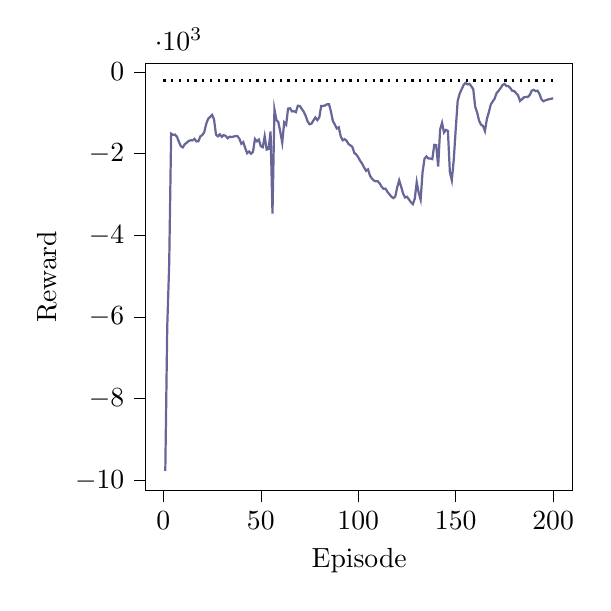
\begin{tikzpicture}

\definecolor{color0}{rgb}{0.12156862745098,0.466666666666667,0.705882352941177}

\begin{axis}[
compat=newest,
tick align=outside,
tick pos=left,
x grid style={white!69.0196078431373!black},
xmin=-8.95, xmax=209.95,
xtick style={color=black},
y grid style={white!69.0196078431373!black},
ymin=-10237.8868910548, ymax=203.619925054467,
ytick style={color=black},
scaled y ticks=true,
scaled y ticks=base 10:-3,
width=7cm,
height=7cm,
xlabel=Episode,
ylabel=Reward
]

\addplot[thick, black, dotted, domain=0:200] {-211.15};

\addplot [thick, blue!20!gray]
table {%
1 -9763.27294486799
2 -6233.80261025401
3 -4702.25607429109
4 -1512.21343297441
5 -1541.56062085325
6 -1535.22850284016
7 -1588.96606184897
8 -1715.23669898396
9 -1820.31231753912
10 -1847.66786072394
11 -1769.92450118555
12 -1734.64730574001
13 -1691.78106317152
14 -1674.45493906621
15 -1676.90591264538
16 -1640.75523295968
17 -1703.4048995174
18 -1697.83044713235
19 -1576.88921890067
20 -1546.5715732237
21 -1474.09512876949
22 -1271.65422689584
23 -1150.29854596291
24 -1102.56488295819
25 -1052.63460403206
26 -1160.0570975787
27 -1531.80428427574
28 -1577.96536228338
29 -1528.46964853933
30 -1588.81698896337
31 -1545.80968137986
32 -1568.85552000374
33 -1624.20152414619
34 -1586.50471460737
35 -1592.55986202214
36 -1584.94638344089
37 -1569.33361174512
38 -1573.1892994717
39 -1633.50494911412
40 -1759.32305467967
41 -1719.13862961987
42 -1862.97480239258
43 -1990.60310329712
44 -1948.10280201805
45 -2003.32412321478
46 -1956.29505058938
47 -1643.40355154487
48 -1699.32053231105
49 -1655.76163636967
50 -1820.85636906421
51 -1844.26667355161
52 -1574.87178814199
53 -1901.6723073915
54 -1886.04289052694
55 -1458.04140202327
56 -3469.32441220565
57 -917.195658586486
58 -1176.59257034398
59 -1230.33078309159
60 -1466.59633331869
61 -1732.22292637077
62 -1236.42594346941
63 -1293.97326214233
64 -899.857651460993
65 -890.845587246339
66 -968.24154739275
67 -963.199443956724
68 -986.677853906075
69 -828.526039545684
70 -834.720257437712
71 -902.709529703026
72 -972.62043534064
73 -1074.17044214855
74 -1209.87366623514
75 -1283.68681382054
76 -1267.54188154102
77 -1187.55869135607
78 -1114.1130550254
79 -1179.99960886007
80 -1115.99943619309
81 -832.657288986692
82 -832.72759717624
83 -822.279758669418
84 -793.164073797469
85 -791.044522604899
86 -972.019086460731
87 -1206.24867561322
88 -1290.02850233563
89 -1384.86591544101
90 -1357.00442247666
91 -1575.38270406248
92 -1674.08821396743
93 -1647.60414166174
94 -1684.15617335132
95 -1765.71695848599
96 -1797.33452011673
97 -1838.75461128161
98 -1985.76014825974
99 -2021.98376684527
100 -2092.02233018191
101 -2178.15994993705
102 -2247.02313410243
103 -2340.33340175948
104 -2420.7367742868
105 -2385.67777225085
106 -2538.2164437452
107 -2609.81411422946
108 -2659.40383450713
109 -2678.50832692135
110 -2676.82744132636
111 -2730.33624432342
112 -2812.33229768694
113 -2861.50305884707
114 -2857.37029123113
115 -2938.78510578548
116 -2994.46766053733
117 -3054.18167696401
118 -3089.68136986634
119 -3050.40051346782
120 -2823.26624003158
121 -2653.39029885552
122 -2806.59146922999
123 -2978.05949681073
124 -3075.60138846972
125 -3056.50890159285
126 -3119.86383000792
127 -3190.77697519937
128 -3237.45041767532
129 -3103.94340263226
130 -2698.75288944802
131 -2956.79624472601
132 -3124.84788885606
133 -2453.99592562811
134 -2125.61227356192
135 -2067.71562137431
136 -2118.05416804509
137 -2120.76157358531
138 -2134.78314728543
139 -1786.15300160098
140 -1793.00208055793
141 -2319.18931540986
142 -1413.05062097296
143 -1245.7107253682
144 -1484.37154592392
145 -1420.74714969691
146 -1446.61374769009
147 -2448.65824563979
148 -2652.9204998935
149 -2151.41685205676
150 -1409.62535384097
151 -715.425293566961
152 -537.233050162036
153 -429.756832729694
154 -325.6823376965
155 -270.994021132317
156 -306.189756950749
157 -292.000625606546
158 -350.489728088838
159 -423.619606641182
160 -855.467889009458
161 -994.472702683325
162 -1195.21463389004
163 -1292.79692031924
164 -1320.56851018644
165 -1448.16350042877
166 -1152.54457203662
167 -987.150718369486
168 -798.086323275897
169 -722.281160318246
170 -651.843048097534
171 -517.090294083444
172 -462.655401350926
173 -399.143888792889
174 -324.173287068825
175 -295.147502477148
176 -344.83352622425
177 -349.652649290451
178 -394.784026316548
179 -462.079584436464
180 -468.014634507583
181 -522.962154721305
182 -573.619728760075
183 -711.92181205646
184 -671.105200941416
185 -622.486488273209
186 -613.495902939192
187 -614.457292613144
188 -566.095980332205
189 -462.064404335876
190 -440.344339674872
191 -470.810273558386
192 -460.606507255502
193 -542.73700519533
194 -671.942780564072
195 -720.097164404344
196 -696.536841144416
197 -680.892791035771
198 -667.588830250088
199 -657.904337807085
200 -646.907259376791
};
\end{axis}

\end{tikzpicture}
}
    \hspace{2.5cm}
    \subfloat[Average reward.]{%
      % This file was created by tikzplotlib v0.9.1.
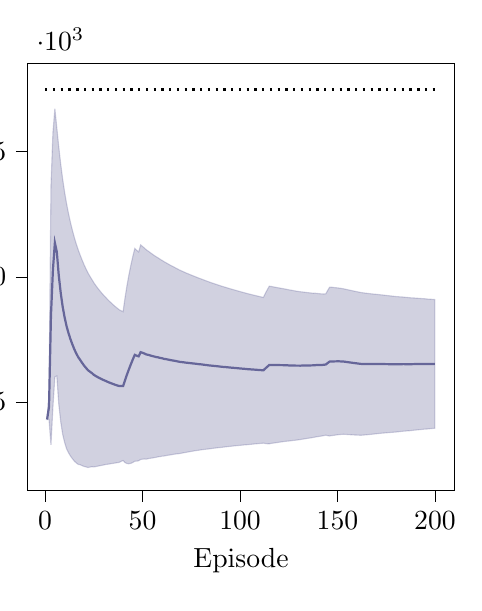
\begin{tikzpicture}[trim axis right,trim axis left]

\definecolor{color0}{rgb}{1,0.498039215686275,0.0549019607843137}
\definecolor{color1}{rgb}{0.12156862745098,0.466666666666667,0.705882352941177}

\begin{axis}[
compat=newest,
tick align=outside,
tick pos=left,
x grid style={white!69.0196078431373!black},
xmin=-8.95, xmax=209.95,
xtick style={color=black},
y grid style={white!69.0196078431373!black},
ymin=-8500, ymax=8500,
ytick style={color=black},
scaled y ticks=true,
scaled y ticks=base 10:-3,
width=7cm,
height=7cm,
xlabel=Episode,
ylabel=Average Reward,
y label style={at={(-0.2,0.5)}}
]

\addplot[thick, black, dotted, domain=0:200] {7461.75};

\path [draw=blue!20!gray, fill=blue!20!gray, opacity=0.3]
(axis cs:1,-5683.54889736257)
--(axis cs:1,-5683.54889736257)
--(axis cs:2,-4664.83596416343)
--(axis cs:3,3611.91015013816)
--(axis cs:4,5733.02874612919)
--(axis cs:5,6703.08679409963)
--(axis cs:6,5941.79779738927)
--(axis cs:7,5181.06295860306)
--(axis cs:8,4495.95947900039)
--(axis cs:9,3896.14664603212)
--(axis cs:10,3376.32312938225)
--(axis cs:11,2920.32294307545)
--(axis cs:12,2525.15744349306)
--(axis cs:13,2171.95496132655)
--(axis cs:14,1855.64226679598)
--(axis cs:15,1566.84923818866)
--(axis cs:16,1307.31486451035)
--(axis cs:17,1070.69485921444)
--(axis cs:18,865.172963604798)
--(axis cs:19,666.607874756861)
--(axis cs:20,482.804895974852)
--(axis cs:21,314.974734842627)
--(axis cs:22,155.659446332147)
--(axis cs:23,21.7160298397339)
--(axis cs:24,-103.627696733365)
--(axis cs:25,-233.036955279191)
--(axis cs:26,-344.647576742026)
--(axis cs:27,-448.279912845569)
--(axis cs:28,-547.517237316667)
--(axis cs:29,-640.829735566254)
--(axis cs:30,-729.086315506914)
--(axis cs:31,-811.631395319951)
--(axis cs:32,-894.282644343613)
--(axis cs:33,-972.142856413599)
--(axis cs:34,-1045.03321156417)
--(axis cs:35,-1116.03381064321)
--(axis cs:36,-1183.19899074506)
--(axis cs:37,-1247.5833211883)
--(axis cs:38,-1309.1740200345)
--(axis cs:39,-1348.94779476236)
--(axis cs:40,-1388.22143226712)
--(axis cs:41,-832.681807583704)
--(axis cs:42,-347.454624180522)
--(axis cs:43,84.0036460116467)
--(axis cs:44,468.613736115966)
--(axis cs:45,816.276437284182)
--(axis cs:46,1132.04168979841)
--(axis cs:47,1058.75280272605)
--(axis cs:48,993.078178500789)
--(axis cs:49,1275.22921923384)
--(axis cs:50,1209.90250609426)
--(axis cs:51,1144.43099871621)
--(axis cs:52,1074.28967068447)
--(axis cs:53,1021.84969181031)
--(axis cs:54,963.284822882199)
--(axis cs:55,906.122375984313)
--(axis cs:56,853.673190284089)
--(axis cs:57,800.474787773306)
--(axis cs:58,754.792361481015)
--(axis cs:59,702.052554214804)
--(axis cs:60,657.200702192931)
--(axis cs:61,605.777553627973)
--(axis cs:62,563.911623111233)
--(axis cs:63,519.849948570358)
--(axis cs:64,475.177789641657)
--(axis cs:65,433.392340412509)
--(axis cs:66,393.703789909052)
--(axis cs:67,353.560947382149)
--(axis cs:68,311.457997567784)
--(axis cs:69,271.135512767131)
--(axis cs:70,236.53417834949)
--(axis cs:71,202.336943876262)
--(axis cs:72,166.771237469463)
--(axis cs:73,134.735395726961)
--(axis cs:74,102.300119821232)
--(axis cs:75,70.5415149877558)
--(axis cs:76,38.8998242521016)
--(axis cs:77,8.97464552618476)
--(axis cs:78,-22.4708054821217)
--(axis cs:79,-53.7952376816515)
--(axis cs:80,-80.6679858663811)
--(axis cs:81,-111.032851575875)
--(axis cs:82,-140.763643927183)
--(axis cs:83,-169.462762129693)
--(axis cs:84,-198.893047108781)
--(axis cs:85,-225.692446338669)
--(axis cs:86,-251.539196494657)
--(axis cs:87,-277.924552937011)
--(axis cs:88,-303.697000827866)
--(axis cs:89,-329.330756837966)
--(axis cs:90,-356.111224723384)
--(axis cs:91,-381.184714059792)
--(axis cs:92,-404.195999696266)
--(axis cs:93,-427.303858793827)
--(axis cs:94,-451.384865611832)
--(axis cs:95,-475.032255001821)
--(axis cs:96,-497.603548377329)
--(axis cs:97,-519.211771923848)
--(axis cs:98,-541.272582843804)
--(axis cs:99,-563.88105569437)
--(axis cs:100,-585.761721153127)
--(axis cs:101,-607.311927425352)
--(axis cs:102,-627.865031243257)
--(axis cs:103,-649.029039005381)
--(axis cs:104,-670.628274582017)
--(axis cs:105,-689.617138377228)
--(axis cs:106,-709.454379164859)
--(axis cs:107,-727.434389108195)
--(axis cs:108,-746.343417065776)
--(axis cs:109,-765.797160678988)
--(axis cs:110,-783.92941074887)
--(axis cs:111,-802.540185305784)
--(axis cs:112,-820.012485104501)
--(axis cs:113,-659.491904486838)
--(axis cs:114,-510.765947503894)
--(axis cs:115,-372.25379264869)
--(axis cs:116,-381.63466107484)
--(axis cs:117,-397.349084447256)
--(axis cs:118,-412.622872398521)
--(axis cs:119,-427.400565002773)
--(axis cs:120,-440.726717489241)
--(axis cs:121,-455.248878102756)
--(axis cs:122,-468.418119542088)
--(axis cs:123,-482.312957038475)
--(axis cs:124,-498.190120384759)
--(axis cs:125,-514.94702411482)
--(axis cs:126,-528.852569547214)
--(axis cs:127,-540.735496322354)
--(axis cs:128,-556.814386191515)
--(axis cs:129,-570.14102094993)
--(axis cs:130,-581.782359374813)
--(axis cs:131,-593.653350383089)
--(axis cs:132,-601.515781135316)
--(axis cs:133,-611.93166274735)
--(axis cs:134,-621.185156621406)
--(axis cs:135,-629.964309509482)
--(axis cs:136,-638.978312806904)
--(axis cs:137,-646.942638411365)
--(axis cs:138,-654.030553328018)
--(axis cs:139,-655.270481440334)
--(axis cs:140,-664.044182267109)
--(axis cs:141,-672.627365453917)
--(axis cs:142,-679.264226520177)
--(axis cs:143,-682.270853033164)
--(axis cs:144,-676.179609271668)
--(axis cs:145,-535.532678327405)
--(axis cs:146,-409.10703793009)
--(axis cs:147,-411.892717803471)
--(axis cs:148,-421.886643796738)
--(axis cs:149,-431.226425078718)
--(axis cs:150,-438.443559640129)
--(axis cs:151,-448.832961296134)
--(axis cs:152,-462.111885336255)
--(axis cs:153,-473.787502508091)
--(axis cs:154,-491.074439689155)
--(axis cs:155,-508.178273268498)
--(axis cs:156,-525.262251102121)
--(axis cs:157,-542.114177466339)
--(axis cs:158,-558.757150489942)
--(axis cs:159,-575.441355335804)
--(axis cs:160,-591.219066137176)
--(axis cs:161,-607.478431196642)
--(axis cs:162,-623.235129955506)
--(axis cs:163,-634.297692200927)
--(axis cs:164,-644.480211434214)
--(axis cs:165,-654.838603405442)
--(axis cs:166,-664.336515971049)
--(axis cs:167,-673.141378223671)
--(axis cs:168,-681.64023579622)
--(axis cs:169,-689.371401014109)
--(axis cs:170,-696.51852122298)
--(axis cs:171,-704.579847351806)
--(axis cs:172,-713.629995994865)
--(axis cs:173,-720.566250020872)
--(axis cs:174,-730.592991023546)
--(axis cs:175,-739.593965263798)
--(axis cs:176,-748.328739205127)
--(axis cs:177,-757.657768142544)
--(axis cs:178,-765.901430865686)
--(axis cs:179,-775.238276040316)
--(axis cs:180,-784.236613202675)
--(axis cs:181,-788.032398170048)
--(axis cs:182,-796.338073103468)
--(axis cs:183,-800.698000145452)
--(axis cs:184,-806.647400905351)
--(axis cs:185,-816.081002827058)
--(axis cs:186,-821.283551232236)
--(axis cs:187,-831.564888999785)
--(axis cs:188,-835.926141988585)
--(axis cs:189,-840.501082580734)
--(axis cs:190,-846.117333717732)
--(axis cs:191,-852.141169682139)
--(axis cs:192,-858.157500729644)
--(axis cs:193,-863.358082117168)
--(axis cs:194,-868.356494583156)
--(axis cs:195,-873.984279746447)
--(axis cs:196,-883.081813687953)
--(axis cs:197,-888.312714201666)
--(axis cs:198,-892.506220919131)
--(axis cs:199,-898.528782160382)
--(axis cs:200,-904.170436091782)
--(axis cs:200,-6031.2460878229)
--(axis cs:200,-6031.2460878229)
--(axis cs:199,-6038.42444692848)
--(axis cs:198,-6045.34935076301)
--(axis cs:197,-6053.86032906361)
--(axis cs:196,-6061.66416558238)
--(axis cs:195,-6065.25582391111)
--(axis cs:194,-6072.91323682603)
--(axis cs:193,-6081.18190232796)
--(axis cs:192,-6089.38541297974)
--(axis cs:191,-6096.99883143657)
--(axis cs:190,-6104.70758222658)
--(axis cs:189,-6112.86796704833)
--(axis cs:188,-6121.93581697468)
--(axis cs:187,-6131.25369105158)
--(axis cs:186,-6134.27128768015)
--(axis cs:185,-6143.17027873174)
--(axis cs:184,-6147.79184367287)
--(axis cs:183,-6156.30310945593)
--(axis cs:182,-6166.12744810052)
--(axis cs:181,-6172.57677505633)
--(axis cs:180,-6182.98453626462)
--(axis cs:179,-6188.88606563874)
--(axis cs:178,-6194.5071756154)
--(axis cs:177,-6201.55352193547)
--(axis cs:176,-6207.4805834666)
--(axis cs:175,-6214.25969044175)
--(axis cs:174,-6220.87745823931)
--(axis cs:173,-6226.37102020022)
--(axis cs:172,-6235.35136223451)
--(axis cs:171,-6242.35822580188)
--(axis cs:170,-6250.56029605835)
--(axis cs:169,-6259.75692027889)
--(axis cs:168,-6268.56223540058)
--(axis cs:167,-6276.76440349625)
--(axis cs:166,-6284.80387771434)
--(axis cs:165,-6292.24997362599)
--(axis cs:164,-6298.8461803169)
--(axis cs:163,-6305.83428797796)
--(axis cs:162,-6311.89046479758)
--(axis cs:161,-6308.64551633529)
--(axis cs:160,-6304.04817807093)
--(axis cs:159,-6301.53490303241)
--(axis cs:158,-6296.27292900861)
--(axis cs:157,-6291.68075968238)
--(axis cs:156,-6286.79003510748)
--(axis cs:155,-6281.50617367602)
--(axis cs:154,-6276.67519043349)
--(axis cs:153,-6271.66681175566)
--(axis cs:152,-6278.75514946603)
--(axis cs:151,-6283.82778001546)
--(axis cs:150,-6292.83128193421)
--(axis cs:149,-6304.92343835404)
--(axis cs:148,-6315.3781087436)
--(axis cs:147,-6325.39608866533)
--(axis cs:146,-6340.84189458265)
--(axis cs:145,-6327.81831465658)
--(axis cs:144,-6306.89965939055)
--(axis cs:143,-6325.11253435764)
--(axis cs:142,-6340.12110683673)
--(axis cs:141,-6353.03092173095)
--(axis cs:140,-6364.58932305702)
--(axis cs:139,-6376.18686354583)
--(axis cs:138,-6392.78251792671)
--(axis cs:137,-6406.13126575647)
--(axis cs:136,-6419.01486662332)
--(axis cs:135,-6431.24748109409)
--(axis cs:134,-6443.90069010564)
--(axis cs:133,-6456.37703998253)
--(axis cs:132,-6468.03981521112)
--(axis cs:131,-6482.09614135046)
--(axis cs:130,-6492.81490908434)
--(axis cs:129,-6504.03840721376)
--(axis cs:128,-6513.70056482159)
--(axis cs:127,-6520.0055803875)
--(axis cs:126,-6531.80294640624)
--(axis cs:125,-6541.69280337811)
--(axis cs:124,-6548.07710001903)
--(axis cs:123,-6556.11608684203)
--(axis cs:122,-6566.96982103314)
--(axis cs:121,-6578.9349093524)
--(axis cs:120,-6589.7391700177)
--(axis cs:119,-6602.18766875233)
--(axis cs:118,-6613.39694392849)
--(axis cs:117,-6624.39238233312)
--(axis cs:116,-6635.23944676604)
--(axis cs:115,-6652.42655535755)
--(axis cs:114,-6649.23260596928)
--(axis cs:113,-6640.67278843788)
--(axis cs:112,-6625.56789396718)
--(axis cs:111,-6633.27170914044)
--(axis cs:110,-6639.69718238966)
--(axis cs:109,-6647.33515888778)
--(axis cs:108,-6653.39246063888)
--(axis cs:107,-6660.82335345178)
--(axis cs:106,-6670.08278996275)
--(axis cs:105,-6677.10981739834)
--(axis cs:104,-6685.93694360195)
--(axis cs:103,-6691.16018034103)
--(axis cs:102,-6697.73713484392)
--(axis cs:101,-6705.86872189792)
--(axis cs:100,-6713.02905834833)
--(axis cs:99,-6720.27792167371)
--(axis cs:98,-6726.97403151993)
--(axis cs:97,-6735.21010057888)
--(axis cs:96,-6744.76523516962)
--(axis cs:95,-6753.53065594397)
--(axis cs:94,-6761.29159862002)
--(axis cs:93,-6769.07621631272)
--(axis cs:92,-6779.09104988975)
--(axis cs:91,-6789.9512747808)
--(axis cs:90,-6798.44178336265)
--(axis cs:89,-6804.87733266241)
--(axis cs:88,-6814.08954486904)
--(axis cs:87,-6823.91767363679)
--(axis cs:86,-6833.64730044682)
--(axis cs:85,-6845.0505844711)
--(axis cs:84,-6855.9145518629)
--(axis cs:83,-6863.46326975569)
--(axis cs:82,-6873.25406853956)
--(axis cs:81,-6882.38557769733)
--(axis cs:80,-6891.5340948193)
--(axis cs:79,-6906.85348314655)
--(axis cs:78,-6916.66883780809)
--(axis cs:77,-6927.44482921364)
--(axis cs:76,-6941.64037869985)
--(axis cs:75,-6954.46684421078)
--(axis cs:74,-6968.31389871547)
--(axis cs:73,-6982.39086047354)
--(axis cs:72,-6998.28127661371)
--(axis cs:71,-7010.20884917465)
--(axis cs:70,-7025.62260861678)
--(axis cs:69,-7041.83872919554)
--(axis cs:68,-7050.35145953409)
--(axis cs:67,-7057.32399564148)
--(axis cs:66,-7069.63771716767)
--(axis cs:65,-7084.41731355485)
--(axis cs:64,-7097.63554062878)
--(axis cs:63,-7107.84849873977)
--(axis cs:62,-7121.18631107269)
--(axis cs:61,-7139.91462246515)
--(axis cs:60,-7144.0255651109)
--(axis cs:59,-7162.31748977068)
--(axis cs:58,-7169.29010654207)
--(axis cs:57,-7190.6723039468)
--(axis cs:56,-7202.43653618954)
--(axis cs:55,-7218.27733110353)
--(axis cs:54,-7228.64953833879)
--(axis cs:53,-7239.59974889705)
--(axis cs:52,-7263.65891887062)
--(axis cs:51,-7256.29345893705)
--(axis cs:50,-7264.57864669187)
--(axis cs:49,-7277.16130265562)
--(axis cs:48,-7327.87082996043)
--(axis cs:47,-7342.93830091869)
--(axis cs:46,-7347.33946452446)
--(axis cs:45,-7394.94018115896)
--(axis cs:44,-7429.54005565069)
--(axis cs:43,-7447.04917501062)
--(axis cs:42,-7440.34838948662)
--(axis cs:41,-7401.85840096014)
--(axis cs:40,-7316.98700665912)
--(axis cs:39,-7353.21111345835)
--(axis cs:38,-7391.92416537074)
--(axis cs:37,-7404.60810131042)
--(axis cs:36,-7417.19550584388)
--(axis cs:35,-7430.06008307852)
--(axis cs:34,-7441.56207713774)
--(axis cs:33,-7455.87504405004)
--(axis cs:32,-7467.56084618186)
--(axis cs:31,-7477.36193897716)
--(axis cs:30,-7495.50826016806)
--(axis cs:29,-7511.54938082628)
--(axis cs:28,-7527.39702695349)
--(axis cs:27,-7542.17888865599)
--(axis cs:26,-7559.87657914347)
--(axis cs:25,-7574.52714205937)
--(axis cs:24,-7563.55722867932)
--(axis cs:23,-7579.94236047905)
--(axis cs:22,-7596.39190182731)
--(axis cs:21,-7573.17902742429)
--(axis cs:20,-7555.14793935344)
--(axis cs:19,-7523.8724538693)
--(axis cs:18,-7486.8550601675)
--(axis cs:17,-7472.85782177765)
--(axis cs:16,-7415.18046242757)
--(axis cs:15,-7344.11905413163)
--(axis cs:14,-7244.7470402469)
--(axis cs:13,-7138.98036628439)
--(axis cs:12,-7006.33538618331)
--(axis cs:11,-6849.89509398383)
--(axis cs:10,-6598.79408408633)
--(axis cs:9,-6272.00834691501)
--(axis cs:8,-5768.96148369249)
--(axis cs:7,-5063.03387118719)
--(axis cs:6,-3948.90904773556)
--(axis cs:5,-3985.04937100994)
--(axis cs:4,-5186.08579412095)
--(axis cs:3,-6695.57327412097)
--(axis cs:2,-5683.54889736257)
--(axis cs:1,-5683.54889736257)
--cycle;

\addplot [thick, blue!20!gray]
table {%
1 -5683.54889736257
2 -5174.192430763
3 -1541.8315619914
4 273.471476004121
5 1359.01871154484
6 996.444374826857
7 59.0145437079384
8 -636.501002346052
9 -1187.93085044144
10 -1611.23547735204
11 -1964.78607545419
12 -2240.58897134512
13 -2483.51270247892
14 -2694.55238672546
15 -2888.63490797148
16 -3053.93279895861
17 -3201.0814812816
18 -3310.84104828135
19 -3428.63228955622
20 -3536.17152168929
21 -3629.10214629083
22 -3720.36622774758
23 -3779.11316531966
24 -3833.59246270634
25 -3903.78204866928
26 -3952.26207794275
27 -3995.22940075078
28 -4037.45713213508
29 -4076.18955819627
30 -4112.29728783748
31 -4144.49666714855
32 -4180.92174526274
33 -4214.00895023182
34 -4243.29764435096
35 -4273.04694686086
36 -4300.19724829447
37 -4326.09571124936
38 -4350.54909270262
39 -4351.07945411036
40 -4352.60421946312
41 -4117.27010427192
42 -3893.90150683357
43 -3681.52276449949
44 -3480.46315976736
45 -3289.33187193739
46 -3107.64888736302
47 -3142.09274909632
48 -3167.39632572982
49 -3000.96604171089
50 -3027.33807029881
51 -3055.93123011042
52 -3094.68462409308
53 -3108.87502854337
54 -3132.6823577283
55 -3156.07747755961
56 -3174.38167295272
57 -3195.09875808675
58 -3207.24887253053
59 -3230.13246777794
60 -3243.41243145899
61 -3267.06853441859
62 -3278.63734398073
63 -3293.9992750847
64 -3311.22887549356
65 -3325.51248657117
66 -3337.96696362931
67 -3351.88152412967
68 -3369.44673098315
69 -3385.3516082142
70 -3394.54421513364
71 -3403.93595264919
72 -3415.75501957212
73 -3423.82773237329
74 -3433.00688944712
75 -3441.96266461151
76 -3451.37027722388
77 -3459.23509184373
78 -3469.56982164511
79 -3480.3243604141
80 -3486.10104034284
81 -3496.7092146366
82 -3507.00885623337
83 -3516.46301594269
84 -3527.40379948584
85 -3535.37151540488
86 -3542.59324847074
87 -3550.9211132869
88 -3558.89327284846
89 -3567.10404475019
90 -3577.27650404302
91 -3585.5679944203
92 -3591.64352479301
93 -3598.19003755328
94 -3606.33823211593
95 -3614.28145547289
96 -3621.18439177348
97 -3627.21093625136
98 -3634.12330718187
99 -3642.07948868404
100 -3649.39538975073
101 -3656.59032466163
102 -3662.80108304359
103 -3670.09460967321
104 -3678.28260909198
105 -3683.36347788778
106 -3689.7685845638
107 -3694.12887127999
108 -3699.86793885233
109 -3706.56615978338
110 -3711.81329656927
111 -3717.90594722311
112 -3722.79018953584
113 -3650.08234646236
114 -3579.99927673659
115 -3512.34017400312
116 -3508.43705392044
117 -3510.87073339019
118 -3513.00990816351
119 -3514.79411687755
120 -3515.23294375347
121 -3517.09189372758
122 -3517.69397028762
123 -3519.21452194025
124 -3523.13361020189
125 -3528.31991374646
126 -3530.32775797673
127 -3530.37053835493
128 -3535.25747550656
129 -3537.08971408184
130 -3537.29863422958
131 -3537.87474586678
132 -3534.77779817322
133 -3534.15435136494
134 -3532.54292336352
135 -3530.60589530179
136 -3528.99658971511
137 -3526.53695208392
138 -3523.40653562737
139 -3515.72867249308
140 -3514.31675266206
141 -3512.82914359243
142 -3509.69266667845
143 -3503.6916936954
144 -3491.53963433111
145 -3431.67549649199
146 -3374.97446625637
147 -3368.6444032344
148 -3368.63237627017
149 -3368.07493171638
150 -3365.63742078717
151 -3366.3303706558
152 -3370.43351740114
153 -3372.72715713188
154 -3383.87481506132
155 -3394.84222347226
156 -3406.0261431048
157 -3416.89746857436
158 -3427.51503974928
159 -3438.48812918411
160 -3447.63362210405
161 -3458.06197376597
162 -3467.56279737654
163 -3470.06599008944
164 -3471.66319587556
165 -3473.54428851571
166 -3474.57019684269
167 -3474.95289085996
168 -3475.1012355984
169 -3474.5641606465
170 -3473.53940864066
171 -3473.46903657684
172 -3474.49067911469
173 -3473.46863511054
174 -3475.73522463143
175 -3476.92682785278
176 -3477.90466133586
177 -3479.60564503901
178 -3480.20430324054
179 -3482.06217083953
180 -3483.61057473365
181 -3480.30458661319
182 -3481.23276060199
183 -3478.50055480069
184 -3477.21962228911
185 -3479.6256407794
186 -3477.77741945619
187 -3481.40929002568
188 -3478.93097948163
189 -3476.68452481453
190 -3475.41245797215
191 -3474.57000055935
192 -3473.77145685469
193 -3472.26999222257
194 -3470.6348657046
195 -3469.62005182878
196 -3472.37298963517
197 -3471.08652163264
198 -3468.92778584107
199 -3468.47661454443
200 -3467.70826195734
};
\end{axis}

\end{tikzpicture}
}
	
	\hspace{1cm}
    \subfloat[Area 1 frequency.]{%
      % This file was created by tikzplotlib v0.9.1.
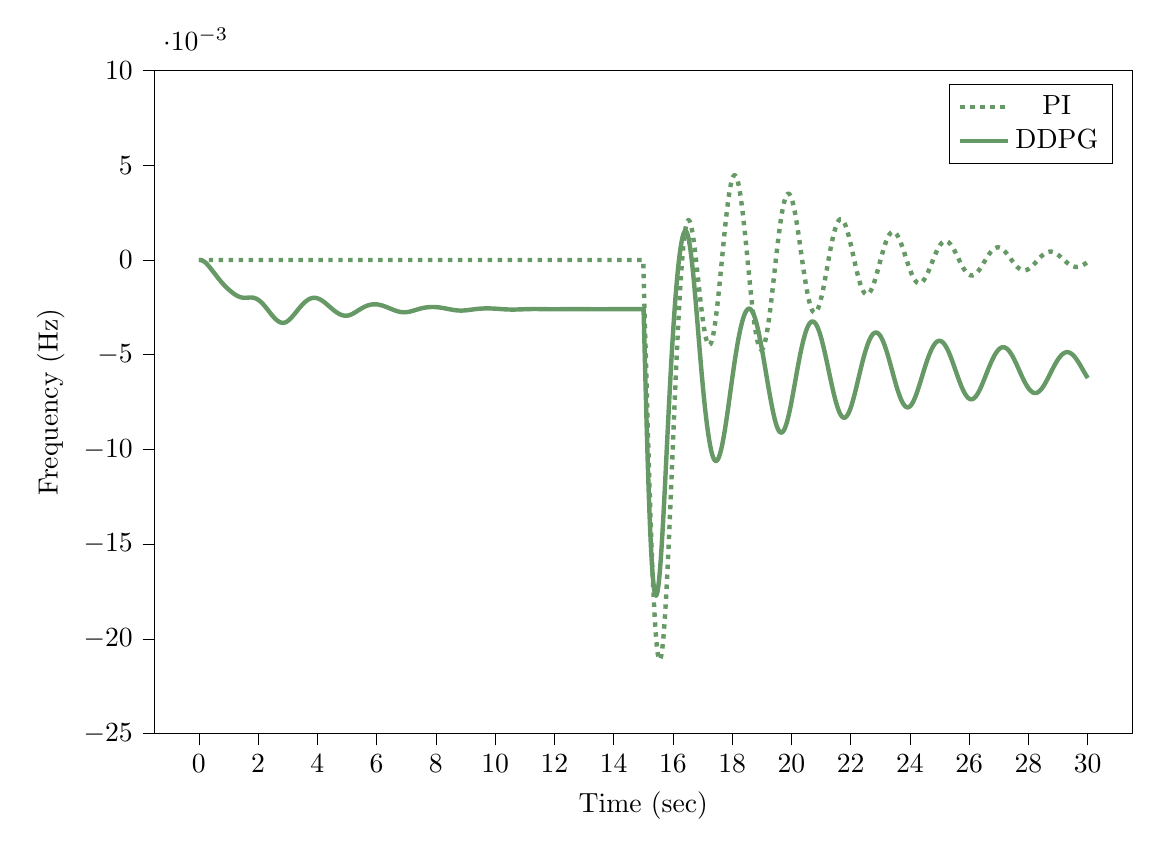
\begin{tikzpicture}

\definecolor{color0}{rgb}{0.12156862745098,0.466666666666667,0.705882352941177}
\definecolor{color1}{rgb}{1,0.498039215686275,0.0549019607843137}

\begin{axis}[
compat=newest,
tick align=outside,
tick pos=left,
x grid style={white!69.0196078431373!black},
xmin=-1.50000000000009, xmax=31.500000000002,
xtick style={color=black},
y grid style={white!69.0196078431373!black},
ymin=-0.025, ymax=0.01,
ytick style={color=black},
%yticklabel style={
%        /pgf/number format/.cd,
%        	fixed,
%        	fixed zerofill,
%         	precision=3,
%        /tikz/.cd
%},
scaled y ticks=true,
scaled y ticks=base 10:3,
width=14cm,
height=10cm,
xlabel=Time (sec),
ylabel=Frequency (Hz)
%y label style={at={(-0.2,0.5)}}
]

\addplot [ultra thick, green!20!gray, dotted]
table {%
0 0
0.01 0
0.02 0
0.03 0
0.04 0
0.05 0
0.06 0
0.07 0
0.08 0
0.09 0
0.1 0
0.11 0
0.12 0
0.13 0
0.14 0
0.15 0
0.16 0
0.17 0
0.18 0
0.19 0
0.2 0
0.21 0
0.22 0
0.23 0
0.24 0
0.25 0
0.26 0
0.27 0
0.28 0
0.29 0
0.3 0
0.31 0
0.32 0
0.33 0
0.34 0
0.35 0
0.36 0
0.37 0
0.38 0
0.39 0
0.4 0
0.41 0
0.42 0
0.43 0
0.44 0
0.45 0
0.46 0
0.47 0
0.48 0
0.49 0
0.5 0
0.51 0
0.52 0
0.53 0
0.54 0
0.55 0
0.56 0
0.57 0
0.58 0
0.59 0
0.6 0
0.61 0
0.62 0
0.63 0
0.64 0
0.65 0
0.66 0
0.67 0
0.68 0
0.69 0
0.7 0
0.71 0
0.72 0
0.73 0
0.74 0
0.75 0
0.76 0
0.77 0
0.78 0
0.79 0
0.8 0
0.81 0
0.820000000000001 0
0.830000000000001 0
0.840000000000001 0
0.850000000000001 0
0.860000000000001 0
0.870000000000001 0
0.880000000000001 0
0.890000000000001 0
0.900000000000001 0
0.910000000000001 0
0.920000000000001 0
0.930000000000001 0
0.940000000000001 0
0.950000000000001 0
0.960000000000001 0
0.970000000000001 0
0.980000000000001 0
0.990000000000001 0
1 0
1.01 0
1.02 0
1.03 0
1.04 0
1.05 0
1.06 0
1.07 0
1.08 0
1.09 0
1.1 0
1.11 0
1.12 0
1.13 0
1.14 0
1.15 0
1.16 0
1.17 0
1.18 0
1.19 0
1.2 0
1.21 0
1.22 0
1.23 0
1.24 0
1.25 0
1.26 0
1.27 0
1.28 0
1.29 0
1.3 0
1.31 0
1.32 0
1.33 0
1.34 0
1.35 0
1.36 0
1.37 0
1.38 0
1.39 0
1.4 0
1.41 0
1.42 0
1.43 0
1.44 0
1.45 0
1.46 0
1.47 0
1.48 0
1.49 0
1.5 0
1.51 0
1.52 0
1.53 0
1.54 0
1.55 0
1.56 0
1.57 0
1.58 0
1.59 0
1.6 0
1.61 0
1.62 0
1.63 0
1.64 0
1.65 0
1.66 0
1.67 0
1.68 0
1.69 0
1.7 0
1.71 0
1.72 0
1.73 0
1.74 0
1.75 0
1.76 0
1.77 0
1.78 0
1.79 0
1.8 0
1.81 0
1.82 0
1.83 0
1.84 0
1.85 0
1.86 0
1.87 0
1.88 0
1.89 0
1.9 0
1.91 0
1.92 0
1.93 0
1.94 0
1.95 0
1.96 0
1.97 0
1.98 0
1.99 0
2 0
2.01 0
2.02 0
2.03 0
2.04 0
2.05 0
2.06 0
2.07 0
2.08 0
2.09 0
2.1 0
2.11 0
2.12 0
2.13 0
2.14 0
2.15 0
2.16 0
2.17 0
2.18 0
2.19 0
2.2 0
2.21 0
2.22 0
2.23 0
2.24 0
2.25 0
2.26 0
2.27 0
2.28 0
2.29 0
2.29999999999999 0
2.30999999999999 0
2.31999999999999 0
2.32999999999999 0
2.33999999999999 0
2.34999999999999 0
2.35999999999999 0
2.36999999999999 0
2.37999999999999 0
2.38999999999999 0
2.39999999999999 0
2.40999999999999 0
2.41999999999999 0
2.42999999999999 0
2.43999999999999 0
2.44999999999999 0
2.45999999999999 0
2.46999999999999 0
2.47999999999999 0
2.48999999999999 0
2.49999999999999 0
2.50999999999999 0
2.51999999999999 0
2.52999999999999 0
2.53999999999999 0
2.54999999999999 0
2.55999999999999 0
2.56999999999999 0
2.57999999999999 0
2.58999999999999 0
2.59999999999999 0
2.60999999999999 0
2.61999999999999 0
2.62999999999999 0
2.63999999999999 0
2.64999999999999 0
2.65999999999999 0
2.66999999999999 0
2.67999999999999 0
2.68999999999999 0
2.69999999999999 0
2.70999999999999 0
2.71999999999999 0
2.72999999999999 0
2.73999999999999 0
2.74999999999999 0
2.75999999999999 0
2.76999999999998 0
2.77999999999998 0
2.78999999999998 0
2.79999999999998 0
2.80999999999998 0
2.81999999999998 0
2.82999999999998 0
2.83999999999998 0
2.84999999999998 0
2.85999999999998 0
2.86999999999998 0
2.87999999999998 0
2.88999999999998 0
2.89999999999998 0
2.90999999999998 0
2.91999999999998 0
2.92999999999998 0
2.93999999999998 0
2.94999999999998 0
2.95999999999998 0
2.96999999999998 0
2.97999999999998 0
2.98999999999998 0
2.99999999999998 0
3.00999999999998 0
3.01999999999998 0
3.02999999999998 0
3.03999999999998 0
3.04999999999998 0
3.05999999999998 0
3.06999999999998 0
3.07999999999998 0
3.08999999999998 0
3.09999999999998 0
3.10999999999998 0
3.11999999999998 0
3.12999999999998 0
3.13999999999998 0
3.14999999999998 0
3.15999999999998 0
3.16999999999998 0
3.17999999999998 0
3.18999999999998 0
3.19999999999998 0
3.20999999999998 0
3.21999999999998 0
3.22999999999998 0
3.23999999999997 0
3.24999999999997 0
3.25999999999997 0
3.26999999999997 0
3.27999999999997 0
3.28999999999997 0
3.29999999999997 0
3.30999999999997 0
3.31999999999997 0
3.32999999999997 0
3.33999999999997 0
3.34999999999997 0
3.35999999999997 0
3.36999999999997 0
3.37999999999997 0
3.38999999999997 0
3.39999999999997 0
3.40999999999997 0
3.41999999999997 0
3.42999999999997 0
3.43999999999997 0
3.44999999999997 0
3.45999999999997 0
3.46999999999997 0
3.47999999999997 0
3.48999999999997 0
3.49999999999997 0
3.50999999999997 0
3.51999999999997 0
3.52999999999997 0
3.53999999999997 0
3.54999999999997 0
3.55999999999997 0
3.56999999999997 0
3.57999999999997 0
3.58999999999997 0
3.59999999999997 0
3.60999999999997 0
3.61999999999997 0
3.62999999999997 0
3.63999999999997 0
3.64999999999997 0
3.65999999999997 0
3.66999999999997 0
3.67999999999997 0
3.68999999999997 0
3.69999999999997 0
3.70999999999996 0
3.71999999999996 0
3.72999999999996 0
3.73999999999996 0
3.74999999999996 0
3.75999999999996 0
3.76999999999996 0
3.77999999999996 0
3.78999999999996 0
3.79999999999996 0
3.80999999999996 0
3.81999999999996 0
3.82999999999996 0
3.83999999999996 0
3.84999999999996 0
3.85999999999996 0
3.86999999999996 0
3.87999999999996 0
3.88999999999996 0
3.89999999999996 0
3.90999999999996 0
3.91999999999996 0
3.92999999999996 0
3.93999999999996 0
3.94999999999996 0
3.95999999999996 0
3.96999999999996 0
3.97999999999996 0
3.98999999999996 0
3.99999999999996 0
4.00999999999996 0
4.01999999999996 0
4.02999999999996 0
4.03999999999996 0
4.04999999999996 0
4.05999999999996 0
4.06999999999996 0
4.07999999999996 0
4.08999999999996 0
4.09999999999996 0
4.10999999999996 0
4.11999999999996 0
4.12999999999996 0
4.13999999999996 0
4.14999999999996 0
4.15999999999996 0
4.16999999999996 0
4.17999999999996 0
4.18999999999996 0
4.19999999999995 0
4.20999999999995 0
4.21999999999995 0
4.22999999999995 0
4.23999999999995 0
4.24999999999995 0
4.25999999999995 0
4.26999999999995 0
4.27999999999995 0
4.28999999999995 0
4.29999999999995 0
4.30999999999995 0
4.31999999999995 0
4.32999999999995 0
4.33999999999995 0
4.34999999999995 0
4.35999999999995 0
4.36999999999995 0
4.37999999999995 0
4.38999999999995 0
4.39999999999995 0
4.40999999999995 0
4.41999999999995 0
4.42999999999995 0
4.43999999999995 0
4.44999999999995 0
4.45999999999995 0
4.46999999999995 0
4.47999999999995 0
4.48999999999995 0
4.49999999999995 0
4.50999999999995 0
4.51999999999995 0
4.52999999999995 0
4.53999999999995 0
4.54999999999995 0
4.55999999999995 0
4.56999999999995 0
4.57999999999995 0
4.58999999999995 0
4.59999999999995 0
4.60999999999995 0
4.61999999999995 0
4.62999999999995 0
4.63999999999995 0
4.64999999999995 0
4.65999999999995 0
4.66999999999994 0
4.67999999999994 0
4.68999999999994 0
4.69999999999994 0
4.70999999999994 0
4.71999999999994 0
4.72999999999994 0
4.73999999999994 0
4.74999999999994 0
4.75999999999994 0
4.76999999999994 0
4.77999999999994 0
4.78999999999994 0
4.79999999999994 0
4.80999999999994 0
4.81999999999994 0
4.82999999999994 0
4.83999999999994 0
4.84999999999994 0
4.85999999999994 0
4.86999999999994 0
4.87999999999994 0
4.88999999999994 0
4.89999999999994 0
4.90999999999994 0
4.91999999999994 0
4.92999999999994 0
4.93999999999994 0
4.94999999999994 0
4.95999999999994 0
4.96999999999994 0
4.97999999999994 0
4.98999999999994 0
4.99999999999994 0
5.00999999999994 0
5.01999999999994 0
5.02999999999994 0
5.03999999999994 0
5.04999999999994 0
5.05999999999994 0
5.06999999999994 0
5.07999999999994 0
5.08999999999994 0
5.09999999999994 0
5.10999999999994 0
5.11999999999994 0
5.12999999999994 0
5.13999999999993 0
5.14999999999993 0
5.15999999999993 0
5.16999999999993 0
5.17999999999993 0
5.18999999999993 0
5.19999999999993 0
5.20999999999993 0
5.21999999999993 0
5.22999999999993 0
5.23999999999993 0
5.24999999999993 0
5.25999999999993 0
5.26999999999993 0
5.27999999999993 0
5.28999999999993 0
5.29999999999993 0
5.30999999999993 0
5.31999999999993 0
5.32999999999993 0
5.33999999999993 0
5.34999999999993 0
5.35999999999993 0
5.36999999999993 0
5.37999999999993 0
5.38999999999993 0
5.39999999999993 0
5.40999999999993 0
5.41999999999993 0
5.42999999999993 0
5.43999999999993 0
5.44999999999993 0
5.45999999999993 0
5.46999999999993 0
5.47999999999993 0
5.48999999999993 0
5.49999999999993 0
5.50999999999993 0
5.51999999999993 0
5.52999999999993 0
5.53999999999993 0
5.54999999999993 0
5.55999999999993 0
5.56999999999993 0
5.57999999999993 0
5.58999999999993 0
5.59999999999993 0
5.60999999999992 0
5.61999999999992 0
5.62999999999992 0
5.63999999999992 0
5.64999999999992 0
5.65999999999992 0
5.66999999999992 0
5.67999999999992 0
5.68999999999992 0
5.69999999999992 0
5.70999999999992 0
5.71999999999992 0
5.72999999999992 0
5.73999999999992 0
5.74999999999992 0
5.75999999999992 0
5.76999999999992 0
5.77999999999992 0
5.78999999999992 0
5.79999999999992 0
5.80999999999992 0
5.81999999999992 0
5.82999999999992 0
5.83999999999992 0
5.84999999999992 0
5.85999999999992 0
5.86999999999992 0
5.87999999999992 0
5.88999999999992 0
5.89999999999992 0
5.90999999999992 0
5.91999999999992 0
5.92999999999992 0
5.93999999999992 0
5.94999999999992 0
5.95999999999992 0
5.96999999999992 0
5.97999999999992 0
5.98999999999992 0
5.99999999999992 0
6.00999999999992 0
6.01999999999992 0
6.02999999999992 0
6.03999999999992 0
6.04999999999992 0
6.05999999999992 0
6.06999999999992 0
6.07999999999991 0
6.08999999999991 0
6.09999999999991 0
6.10999999999991 0
6.11999999999991 0
6.12999999999991 0
6.13999999999991 0
6.14999999999991 0
6.15999999999991 0
6.16999999999991 0
6.17999999999991 0
6.18999999999991 0
6.19999999999991 0
6.20999999999991 0
6.21999999999991 0
6.22999999999991 0
6.23999999999991 0
6.24999999999991 0
6.25999999999991 0
6.26999999999991 0
6.27999999999991 0
6.28999999999991 0
6.29999999999991 0
6.30999999999991 0
6.31999999999991 0
6.32999999999991 0
6.33999999999991 0
6.34999999999991 0
6.35999999999991 0
6.36999999999991 0
6.37999999999991 0
6.38999999999991 0
6.39999999999991 0
6.40999999999991 0
6.41999999999991 0
6.42999999999991 0
6.43999999999991 0
6.44999999999991 0
6.45999999999991 0
6.46999999999991 0
6.47999999999991 0
6.48999999999991 0
6.49999999999991 0
6.50999999999991 0
6.51999999999991 0
6.52999999999991 0
6.53999999999991 0
6.5499999999999 0
6.5599999999999 0
6.5699999999999 0
6.5799999999999 0
6.5899999999999 0
6.5999999999999 0
6.6099999999999 0
6.6199999999999 0
6.6299999999999 0
6.6399999999999 0
6.6499999999999 0
6.6599999999999 0
6.6699999999999 0
6.6799999999999 0
6.6899999999999 0
6.6999999999999 0
6.7099999999999 0
6.7199999999999 0
6.7299999999999 0
6.7399999999999 0
6.7499999999999 0
6.7599999999999 0
6.7699999999999 0
6.7799999999999 0
6.7899999999999 0
6.7999999999999 0
6.8099999999999 0
6.8199999999999 0
6.8299999999999 0
6.8399999999999 0
6.8499999999999 0
6.8599999999999 0
6.8699999999999 0
6.8799999999999 0
6.8899999999999 0
6.8999999999999 0
6.9099999999999 0
6.9199999999999 0
6.9299999999999 0
6.9399999999999 0
6.9499999999999 0
6.9599999999999 0
6.9699999999999 0
6.9799999999999 0
6.9899999999999 0
6.9999999999999 0
7.00999999999989 0
7.01999999999989 0
7.02999999999989 0
7.03999999999989 0
7.04999999999989 0
7.05999999999989 0
7.06999999999989 0
7.07999999999989 0
7.08999999999989 0
7.09999999999989 0
7.10999999999989 0
7.11999999999989 0
7.12999999999989 0
7.13999999999989 0
7.14999999999989 0
7.15999999999989 0
7.16999999999989 0
7.17999999999989 0
7.18999999999989 0
7.19999999999989 0
7.20999999999989 0
7.21999999999989 0
7.22999999999989 0
7.23999999999989 0
7.24999999999989 0
7.25999999999989 0
7.26999999999989 0
7.27999999999989 0
7.28999999999989 0
7.29999999999989 0
7.30999999999989 0
7.31999999999989 0
7.32999999999989 0
7.33999999999989 0
7.34999999999989 0
7.35999999999989 0
7.36999999999989 0
7.37999999999989 0
7.38999999999989 0
7.39999999999989 0
7.40999999999989 0
7.41999999999989 0
7.42999999999989 0
7.43999999999989 0
7.44999999999989 0
7.45999999999989 0
7.46999999999989 0
7.47999999999988 0
7.48999999999988 0
7.49999999999988 0
7.50999999999988 0
7.51999999999988 0
7.52999999999988 0
7.53999999999988 0
7.54999999999988 0
7.55999999999988 0
7.56999999999988 0
7.57999999999988 0
7.58999999999988 0
7.59999999999988 0
7.60999999999988 0
7.61999999999988 0
7.62999999999988 0
7.63999999999988 0
7.64999999999988 0
7.65999999999988 0
7.66999999999988 0
7.67999999999988 0
7.68999999999988 0
7.69999999999988 0
7.70999999999988 0
7.71999999999988 0
7.72999999999988 0
7.73999999999988 0
7.74999999999988 0
7.75999999999988 0
7.76999999999988 0
7.77999999999988 0
7.78999999999988 0
7.79999999999988 0
7.80999999999988 0
7.81999999999988 0
7.82999999999988 0
7.83999999999988 0
7.84999999999988 0
7.85999999999988 0
7.86999999999988 0
7.87999999999988 0
7.88999999999988 0
7.89999999999988 0
7.90999999999988 0
7.91999999999988 0
7.92999999999988 0
7.93999999999988 0
7.94999999999987 0
7.95999999999987 0
7.96999999999987 0
7.97999999999987 0
7.98999999999987 0
7.99999999999987 0
8.00999999999987 0
8.01999999999987 0
8.02999999999987 0
8.03999999999987 0
8.04999999999987 0
8.05999999999987 0
8.06999999999987 0
8.07999999999987 0
8.08999999999987 0
8.09999999999987 0
8.10999999999987 0
8.11999999999987 0
8.12999999999987 0
8.13999999999987 0
8.14999999999987 0
8.15999999999987 0
8.16999999999987 0
8.17999999999987 0
8.18999999999987 0
8.19999999999987 0
8.20999999999987 0
8.21999999999987 0
8.22999999999987 0
8.23999999999987 0
8.24999999999987 0
8.25999999999987 0
8.26999999999987 0
8.27999999999987 0
8.28999999999987 0
8.29999999999987 0
8.30999999999987 0
8.31999999999987 0
8.32999999999987 0
8.33999999999987 0
8.34999999999987 0
8.35999999999987 0
8.36999999999987 0
8.37999999999987 0
8.38999999999987 0
8.39999999999987 0
8.40999999999987 0
8.41999999999986 0
8.42999999999986 0
8.43999999999986 0
8.44999999999986 0
8.45999999999986 0
8.46999999999986 0
8.47999999999986 0
8.48999999999986 0
8.49999999999986 0
8.50999999999986 0
8.51999999999986 0
8.52999999999986 0
8.53999999999986 0
8.54999999999986 0
8.55999999999986 0
8.56999999999986 0
8.57999999999986 0
8.58999999999986 0
8.59999999999986 0
8.60999999999986 0
8.61999999999986 0
8.62999999999986 0
8.63999999999986 0
8.64999999999986 0
8.65999999999986 0
8.66999999999986 0
8.67999999999986 0
8.68999999999986 0
8.69999999999986 0
8.70999999999986 0
8.71999999999986 0
8.72999999999986 0
8.73999999999986 0
8.74999999999986 0
8.75999999999986 0
8.76999999999986 0
8.77999999999986 0
8.78999999999986 0
8.79999999999986 0
8.80999999999986 0
8.81999999999986 0
8.82999999999986 0
8.83999999999986 0
8.84999999999986 0
8.85999999999986 0
8.86999999999986 0
8.87999999999986 0
8.88999999999985 0
8.89999999999985 0
8.90999999999985 0
8.91999999999985 0
8.92999999999985 0
8.93999999999985 0
8.94999999999985 0
8.95999999999985 0
8.96999999999985 0
8.97999999999985 0
8.98999999999985 0
8.99999999999985 0
9.00999999999985 0
9.01999999999985 0
9.02999999999985 0
9.03999999999985 0
9.04999999999985 0
9.05999999999985 0
9.06999999999985 0
9.07999999999985 0
9.08999999999985 0
9.09999999999985 0
9.10999999999985 0
9.11999999999985 0
9.12999999999985 0
9.13999999999985 0
9.14999999999985 0
9.15999999999985 0
9.16999999999985 0
9.17999999999985 0
9.18999999999985 0
9.19999999999985 0
9.20999999999985 0
9.21999999999985 0
9.22999999999985 0
9.23999999999985 0
9.24999999999985 0
9.25999999999985 0
9.26999999999985 0
9.27999999999985 0
9.28999999999985 0
9.29999999999985 0
9.30999999999985 0
9.31999999999985 0
9.32999999999985 0
9.33999999999985 0
9.34999999999985 0
9.35999999999984 0
9.36999999999984 0
9.37999999999984 0
9.38999999999984 0
9.39999999999984 0
9.40999999999984 0
9.41999999999984 0
9.42999999999984 0
9.43999999999984 0
9.44999999999984 0
9.45999999999984 0
9.46999999999984 0
9.47999999999984 0
9.48999999999984 0
9.49999999999984 0
9.50999999999984 0
9.51999999999984 0
9.52999999999984 0
9.53999999999984 0
9.54999999999984 0
9.55999999999984 0
9.56999999999984 0
9.57999999999984 0
9.58999999999984 0
9.59999999999984 0
9.60999999999984 0
9.61999999999984 0
9.62999999999984 0
9.63999999999984 0
9.64999999999984 0
9.65999999999984 0
9.66999999999984 0
9.67999999999984 0
9.68999999999984 0
9.69999999999984 0
9.70999999999984 0
9.71999999999984 0
9.72999999999984 0
9.73999999999984 0
9.74999999999984 0
9.75999999999984 0
9.76999999999984 0
9.77999999999984 0
9.78999999999984 0
9.79999999999984 0
9.80999999999984 0
9.81999999999984 0
9.82999999999983 0
9.83999999999983 0
9.84999999999983 0
9.85999999999983 0
9.86999999999983 0
9.87999999999983 0
9.88999999999983 0
9.89999999999983 0
9.90999999999983 0
9.91999999999983 0
9.92999999999983 0
9.93999999999983 0
9.94999999999983 0
9.95999999999983 0
9.96999999999983 0
9.97999999999983 0
9.98999999999983 0
9.99999999999983 0
10.0099999999998 0
10.0199999999998 0
10.0299999999998 0
10.0399999999998 0
10.0499999999998 0
10.0599999999998 0
10.0699999999998 0
10.0799999999998 0
10.0899999999998 0
10.0999999999998 0
10.1099999999998 0
10.1199999999998 0
10.1299999999998 0
10.1399999999998 0
10.1499999999998 0
10.1599999999998 0
10.1699999999998 0
10.1799999999998 0
10.1899999999998 0
10.1999999999998 0
10.2099999999998 0
10.2199999999998 0
10.2299999999998 0
10.2399999999998 0
10.2499999999998 0
10.2599999999998 0
10.2699999999998 0
10.2799999999998 0
10.2899999999998 0
10.2999999999998 0
10.3099999999998 0
10.3199999999998 0
10.3299999999998 0
10.3399999999998 0
10.3499999999998 0
10.3599999999998 0
10.3699999999998 0
10.3799999999998 0
10.3899999999998 0
10.3999999999998 0
10.4099999999998 0
10.4199999999998 0
10.4299999999998 0
10.4399999999998 0
10.4499999999998 0
10.4599999999998 0
10.4699999999998 0
10.4799999999998 0
10.4899999999998 0
10.4999999999998 0
10.5099999999998 0
10.5199999999998 0
10.5299999999998 0
10.5399999999998 0
10.5499999999998 0
10.5599999999998 0
10.5699999999998 0
10.5799999999998 0
10.5899999999998 0
10.5999999999998 0
10.6099999999998 0
10.6199999999998 0
10.6299999999998 0
10.6399999999998 0
10.6499999999998 0
10.6599999999998 0
10.6699999999998 0
10.6799999999998 0
10.6899999999998 0
10.6999999999998 0
10.7099999999998 0
10.7199999999998 0
10.7299999999998 0
10.7399999999998 0
10.7499999999998 0
10.7599999999998 0
10.7699999999998 0
10.7799999999998 0
10.7899999999998 0
10.7999999999998 0
10.8099999999998 0
10.8199999999998 0
10.8299999999998 0
10.8399999999998 0
10.8499999999998 0
10.8599999999998 0
10.8699999999998 0
10.8799999999998 0
10.8899999999998 0
10.8999999999998 0
10.9099999999998 0
10.9199999999998 0
10.9299999999998 0
10.9399999999998 0
10.9499999999998 0
10.9599999999998 0
10.9699999999998 0
10.9799999999998 0
10.9899999999998 0
10.9999999999998 0
11.0099999999998 0
11.0199999999998 0
11.0299999999998 0
11.0399999999998 0
11.0499999999998 0
11.0599999999998 0
11.0699999999998 0
11.0799999999998 0
11.0899999999998 0
11.0999999999998 0
11.1099999999998 0
11.1199999999998 0
11.1299999999998 0
11.1399999999998 0
11.1499999999998 0
11.1599999999998 0
11.1699999999998 0
11.1799999999998 0
11.1899999999998 0
11.1999999999998 0
11.2099999999998 0
11.2199999999998 0
11.2299999999998 0
11.2399999999998 0
11.2499999999998 0
11.2599999999998 0
11.2699999999998 0
11.2799999999998 0
11.2899999999998 0
11.2999999999998 0
11.3099999999998 0
11.3199999999998 0
11.3299999999998 0
11.3399999999998 0
11.3499999999998 0
11.3599999999998 0
11.3699999999998 0
11.3799999999998 0
11.3899999999998 0
11.3999999999998 0
11.4099999999998 0
11.4199999999998 0
11.4299999999998 0
11.4399999999998 0
11.4499999999998 0
11.4599999999998 0
11.4699999999998 0
11.4799999999998 0
11.4899999999998 0
11.4999999999998 0
11.5099999999998 0
11.5199999999998 0
11.5299999999998 0
11.5399999999998 0
11.5499999999998 0
11.5599999999998 0
11.5699999999998 0
11.5799999999998 0
11.5899999999998 0
11.5999999999998 0
11.6099999999998 0
11.6199999999998 0
11.6299999999998 0
11.6399999999998 0
11.6499999999998 0
11.6599999999998 0
11.6699999999998 0
11.6799999999998 0
11.6899999999998 0
11.6999999999998 0
11.7099999999998 0
11.7199999999998 0
11.7299999999998 0
11.7399999999998 0
11.7499999999998 0
11.7599999999998 0
11.7699999999998 0
11.7799999999998 0
11.7899999999998 0
11.7999999999998 0
11.8099999999998 0
11.8199999999998 0
11.8299999999998 0
11.8399999999998 0
11.8499999999998 0
11.8599999999998 0
11.8699999999998 0
11.8799999999998 0
11.8899999999998 0
11.8999999999998 0
11.9099999999998 0
11.9199999999998 0
11.9299999999998 0
11.9399999999998 0
11.9499999999998 0
11.9599999999998 0
11.9699999999998 0
11.9799999999998 0
11.9899999999998 0
11.9999999999998 0
12.0099999999998 0
12.0199999999998 0
12.0299999999998 0
12.0399999999998 0
12.0499999999998 0
12.0599999999998 0
12.0699999999998 0
12.0799999999998 0
12.0899999999998 0
12.0999999999998 0
12.1099999999998 0
12.1199999999998 0
12.1299999999998 0
12.1399999999998 0
12.1499999999998 0
12.1599999999998 0
12.1699999999998 0
12.1799999999998 0
12.1899999999998 0
12.1999999999998 0
12.2099999999998 0
12.2199999999998 0
12.2299999999998 0
12.2399999999998 0
12.2499999999998 0
12.2599999999998 0
12.2699999999998 0
12.2799999999998 0
12.2899999999998 0
12.2999999999998 0
12.3099999999998 0
12.3199999999998 0
12.3299999999998 0
12.3399999999998 0
12.3499999999998 0
12.3599999999998 0
12.3699999999998 0
12.3799999999998 0
12.3899999999998 0
12.3999999999998 0
12.4099999999998 0
12.4199999999998 0
12.4299999999998 0
12.4399999999998 0
12.4499999999998 0
12.4599999999998 0
12.4699999999998 0
12.4799999999998 0
12.4899999999998 0
12.4999999999998 0
12.5099999999998 0
12.5199999999998 0
12.5299999999998 0
12.5399999999998 0
12.5499999999998 0
12.5599999999998 0
12.5699999999998 0
12.5799999999998 0
12.5899999999998 0
12.5999999999998 0
12.6099999999998 0
12.6199999999998 0
12.6299999999998 0
12.6399999999998 0
12.6499999999998 0
12.6599999999998 0
12.6699999999998 0
12.6799999999998 0
12.6899999999998 0
12.6999999999998 0
12.7099999999998 0
12.7199999999998 0
12.7299999999998 0
12.7399999999998 0
12.7499999999998 0
12.7599999999998 0
12.7699999999998 0
12.7799999999998 0
12.7899999999998 0
12.7999999999998 0
12.8099999999998 0
12.8199999999998 0
12.8299999999998 0
12.8399999999998 0
12.8499999999998 0
12.8599999999998 0
12.8699999999998 0
12.8799999999998 0
12.8899999999998 0
12.8999999999998 0
12.9099999999998 0
12.9199999999998 0
12.9299999999998 0
12.9399999999998 0
12.9499999999998 0
12.9599999999998 0
12.9699999999998 0
12.9799999999998 0
12.9899999999998 0
12.9999999999998 0
13.0099999999998 0
13.0199999999998 0
13.0299999999998 0
13.0399999999998 0
13.0499999999998 0
13.0599999999998 0
13.0699999999998 0
13.0799999999998 0
13.0899999999998 0
13.0999999999998 0
13.1099999999998 0
13.1199999999998 0
13.1299999999998 0
13.1399999999998 0
13.1499999999998 0
13.1599999999998 0
13.1699999999998 0
13.1799999999998 0
13.1899999999998 0
13.1999999999998 0
13.2099999999998 0
13.2199999999998 0
13.2299999999998 0
13.2399999999998 0
13.2499999999998 0
13.2599999999998 0
13.2699999999998 0
13.2799999999998 0
13.2899999999998 0
13.2999999999998 0
13.3099999999998 0
13.3199999999998 0
13.3299999999998 0
13.3399999999998 0
13.3499999999998 0
13.3599999999998 0
13.3699999999998 0
13.3799999999998 0
13.3899999999998 0
13.3999999999998 0
13.4099999999998 0
13.4199999999998 0
13.4299999999998 0
13.4399999999998 0
13.4499999999998 0
13.4599999999998 0
13.4699999999998 0
13.4799999999998 0
13.4899999999998 0
13.4999999999998 0
13.5099999999998 0
13.5199999999998 0
13.5299999999998 0
13.5399999999998 0
13.5499999999998 0
13.5599999999998 0
13.5699999999998 0
13.5799999999998 0
13.5899999999998 0
13.5999999999998 0
13.6099999999998 0
13.6199999999998 0
13.6299999999998 0
13.6399999999998 0
13.6499999999998 0
13.6599999999998 0
13.6699999999998 0
13.6799999999998 0
13.6899999999998 0
13.6999999999998 0
13.7099999999998 0
13.7199999999998 0
13.7299999999998 0
13.7399999999998 0
13.7499999999998 0
13.7599999999998 0
13.7699999999998 0
13.7799999999998 0
13.7899999999998 0
13.7999999999998 0
13.8099999999998 0
13.8199999999997 0
13.8299999999997 0
13.8399999999997 0
13.8499999999997 0
13.8599999999997 0
13.8699999999997 0
13.8799999999997 0
13.8899999999997 0
13.8999999999997 0
13.9099999999997 0
13.9199999999997 0
13.9299999999997 0
13.9399999999997 0
13.9499999999997 0
13.9599999999997 0
13.9699999999997 0
13.9799999999997 0
13.9899999999997 0
13.9999999999997 0
14.0099999999997 0
14.0199999999997 0
14.0299999999997 0
14.0399999999997 0
14.0499999999997 0
14.0599999999997 0
14.0699999999997 0
14.0799999999997 0
14.0899999999997 0
14.0999999999997 0
14.1099999999997 0
14.1199999999997 0
14.1299999999997 0
14.1399999999997 0
14.1499999999997 0
14.1599999999997 0
14.1699999999997 0
14.1799999999997 0
14.1899999999997 0
14.1999999999997 0
14.2099999999997 0
14.2199999999997 0
14.2299999999997 0
14.2399999999997 0
14.2499999999997 0
14.2599999999997 0
14.2699999999997 0
14.2799999999997 0
14.2899999999997 0
14.2999999999997 0
14.3099999999997 0
14.3199999999997 0
14.3299999999997 0
14.3399999999997 0
14.3499999999997 0
14.3599999999997 0
14.3699999999997 0
14.3799999999997 0
14.3899999999997 0
14.3999999999997 0
14.4099999999997 0
14.4199999999997 0
14.4299999999997 0
14.4399999999997 0
14.4499999999997 0
14.4599999999997 0
14.4699999999997 0
14.4799999999997 0
14.4899999999997 0
14.4999999999997 0
14.5099999999997 0
14.5199999999997 0
14.5299999999997 0
14.5399999999997 0
14.5499999999997 0
14.5599999999997 0
14.5699999999997 0
14.5799999999997 0
14.5899999999997 0
14.5999999999997 0
14.6099999999997 0
14.6199999999997 0
14.6299999999997 0
14.6399999999997 0
14.6499999999997 0
14.6599999999997 0
14.6699999999997 0
14.6799999999997 0
14.6899999999997 0
14.6999999999997 0
14.7099999999997 0
14.7199999999997 0
14.7299999999997 0
14.7399999999997 0
14.7499999999997 0
14.7599999999997 0
14.7699999999997 0
14.7799999999997 0
14.7899999999997 0
14.7999999999997 0
14.8099999999997 0
14.8199999999997 0
14.8299999999997 0
14.8399999999997 0
14.8499999999997 0
14.8599999999997 0
14.8699999999997 0
14.8799999999997 0
14.8899999999997 0
14.8999999999997 0
14.9099999999997 0
14.9199999999997 0
14.9299999999997 0
14.9399999999997 0
14.9499999999997 0
14.9599999999997 0
14.9699999999997 0
14.9799999999997 0
14.9899999999997 0
14.9999999999997 -3.93651211614443e-09
15.0099999999997 -0.000599816270682417
15.0199999999997 -0.00119908880084479
15.0299999999997 -0.00179754253372852
15.0399999999997 -0.0023948446344429
15.0499999999997 -0.00299062124939138
15.0599999999997 -0.00358446368618463
15.0699999999997 -0.00417593452179766
15.0799999999997 -0.00476457277282835
15.0899999999997 -0.00534989852308608
15.0999999999997 -0.00593141709971282
15.1099999999997 -0.00650862278845816
15.1199999999997 -0.00708100214101138
15.1299999999997 -0.00764803692388741
15.1399999999997 -0.00820920675160281
15.1499999999997 -0.00876399144127596
15.1599999999997 -0.00931187312100392
15.1699999999997 -0.00985233812025386
15.1799999999997 -0.0103848786669187
15.1899999999997 -0.0109089944125681
15.1999999999997 -0.0114241938047095
15.2099999999997 -0.0119299953224874
15.2199999999997 -0.0124259285901838
15.2299999999997 -0.0129115353810624
15.2399999999997 -0.0133863705225182
15.2499999999997 -0.0138500027121151
15.2599999999997 -0.0143020152528775
15.2699999999997 -0.0147420067151584
15.2799999999997 -0.0151695915314819
15.2899999999997 -0.0155844005299559
15.2999999999997 -0.0159860814111557
15.3099999999997 -0.0163742991727683
15.3199999999997 -0.0167487364857575
15.3299999999997 -0.0171090940253509
15.3399999999997 -0.0174550907597512
15.3499999999997 -0.0177864641991206
15.3599999999997 -0.0181029706070963
15.3699999999997 -0.0184043851768254
15.3799999999997 -0.0186905021732893
15.3899999999997 -0.0189611350434885
15.3999999999997 -0.0192161164958972
15.4099999999997 -0.0194552985504484
15.4199999999997 -0.0196785525601916
15.4299999999997 -0.0198857692056582
15.4399999999997 -0.0200768584641575
15.4499999999997 -0.0202517495499544
15.4599999999997 -0.0204103908330175
15.4699999999997 -0.0205527497331997
15.4799999999997 -0.0206788125911258
15.4899999999997 -0.020788584517633
15.4999999999997 -0.0208820892175594
15.5099999999997 -0.0209593687961681
15.5199999999997 -0.0210204835436248
15.5299999999997 -0.0210655116994115
15.5399999999997 -0.0210945491972521
15.5499999999997 -0.0211077093911169
15.5599999999997 -0.0211051227628629
15.5699999999997 -0.0210869366120657
15.5799999999997 -0.0210533147283251
15.5899999999997 -0.0210044370457204
15.5999999999997 -0.020940499661103
15.6099999999997 -0.02086171413124
15.6199999999997 -0.0207683066693864
15.6299999999997 -0.020660518109462
15.6399999999997 -0.0205386034887037
15.6499999999997 -0.0204028316172527
15.6599999999997 -0.0202534846352881
15.6699999999997 -0.0200908575583267
15.6799999999997 -0.0199152578113132
15.6899999999997 -0.0197270047521316
15.6999999999997 -0.0195264291881473
15.7099999999997 -0.0193138729363691
15.7199999999997 -0.0190896890340603
15.7299999999997 -0.0188542395663603
15.7399999999997 -0.0186078960302049
15.7499999999997 -0.0183510388078863
15.7599999999997 -0.0180840566345368
15.7699999999997 -0.0178073460601992
15.7799999999997 -0.0175213109087395
15.7899999999997 -0.0172263617280233
15.7999999999997 -0.016922915240841
15.8099999999997 -0.01661139379293
15.8199999999997 -0.0162922247980807
15.8299999999997 -0.0159658401796997
15.8399999999997 -0.0156326758149685
15.8499999999997 -0.0152931709775959
15.8599999999997 -0.0149477677811284
15.8699999999997 -0.0145969106234627
15.8799999999997 -0.0142410456332094
15.8899999999997 -0.0138806201185429
15.8999999999997 -0.0135160820191715
15.9099999999997 -0.0131478793620514
15.9199999999997 -0.0127764597214612
15.9299999999997 -0.0124022696846984
15.9399999999997 -0.0120257543239688
15.9499999999997 -0.0116473566690436
15.9599999999997 -0.0112675171929203
15.9699999999997 -0.0108866733026251
15.9799999999997 -0.010505258837876
15.9899999999997 -0.0101237035781487
15.9999999999997 -0.00974243275867871
16.0099999999997 -0.00936186659591788
16.0199999999997 -0.00898241982295028
16.0299999999997 -0.00860450123535923
16.0399999999997 -0.00822851324802252
16.0499999999997 -0.00785485146330229
16.0599999999997 -0.00748390425088176
16.0699999999997 -0.00711605208197563
16.0799999999997 -0.00675166756085005
16.0899999999997 -0.00639111487612701
16.0999999999997 -0.00603474943086742
16.1099999999997 -0.00568291748648845
16.1199999999997 -0.00533595582082919
16.1299999999997 -0.00499419140065999
16.1399999999997 -0.00465794106892187
16.1499999999997 -0.00432751124696018
16.1599999999997 -0.00400319765199849
16.1699999999997 -0.00368528503008679
16.1799999999997 -0.0033740469047313
16.1899999999997 -0.00306974534139794
16.1999999999997 -0.00277263072806533
16.2099999999997 -0.00248294157197574
16.2199999999997 -0.00220090431271978
16.2299999999997 -0.00192673315176691
16.2399999999997 -0.0016606298985342
16.2499999999997 -0.00140278383306765
16.2599999999997 -0.00115337158538734
16.2699999999997 -0.000912557031531131
16.2799999999997 -0.000680491206307545
16.2899999999997 -0.000457312232753518
16.2999999999997 -0.000243145268269894
16.3099999999998 -3.81024673904882e-05
16.3199999999998 0.00015771713102514
16.3299999999998 0.000344227673721556
16.3399999999998 0.000521356105297853
16.3499999999998 0.000689042358774393
16.3599999999998 0.000847239440588993
16.3699999999998 0.00099591332670907
16.3799999999998 0.00113504259012152
16.3899999999998 0.00126461852068281
16.3999999999998 0.00138464501860784
16.4099999999998 0.00149513847296923
16.4199999999998 0.0015961276241521
16.4299999999998 0.00168765341074405
16.4399999999998 0.0017697688146495
16.4499999999998 0.00184253867514877
16.4599999999998 0.0019060394962789
16.4699999999998 0.00196035924092799
16.4799999999998 0.00200559710878891
16.4899999999998 0.00204186330986465
16.4999999999998 0.002069278825239
16.5099999999998 0.00208797514479422
16.5199999999998 0.00209809400051514
16.5299999999998 0.00209978802941269
16.5399999999998 0.00209321888857385
16.5499999999998 0.00207855719233783
16.5599999999998 0.00205598263621555
16.5699999999998 0.00202568367722203
16.5799999999998 0.00198785720589268
16.5899999999998 0.00194270821034066
16.5999999999998 0.00189044943275088
16.6099999999998 0.0018313010187348
16.6199999999998 0.00176549015999127
16.6299999999998 0.00169325073073661
16.6399999999998 0.00161482291837872
16.6499999999998 0.00153045285311375
16.6599999999998 0.00144039222069301
16.6699999999998 0.00134489788207572
16.6799999999998 0.00124423148626304
16.6899999999998 0.00113865907963004
16.6999999999998 0.00102845071250492
16.7099999999998 0.000913880043508624
16.7199999999998 0.00079522394216759
16.7299999999998 0.000672762090313417
16.7399999999998 0.000546776582781965
16.7499999999998 0.000417551527921705
16.7599999999998 0.000285372648420103
16.7699999999998 0.000150526882953243
16.7799999999998 1.33019891587028e-05
16.7899999999998 -0.000126013851577711
16.7999999999998 -0.00026713242708048
16.8099999999998 -0.000409765884387918
16.8199999999998 -0.000553627116548537
16.8299999999998 -0.000698430145693409
16.8399999999998 -0.000843890501892508
16.8499999999998 -0.00098972559733667
16.8599999999998 -0.00113565509539701
16.8699999999998 -0.0012814012741216
16.8799999999998 -0.00142668938373918
16.8899999999998 -0.00157124799775024
16.8999999999998 -0.00171480935719467
16.9099999999998 -0.00185710970769842
16.9199999999998 -0.00199788962890912
16.9299999999998 -0.00213689435595583
16.9399999999998 -0.00227387409255594
16.9499999999999 -0.0024085843154265
16.9599999999999 -0.00254078606962648
16.9699999999999 -0.0026702462544885
16.9799999999999 -0.00279673790004541
16.9899999999999 -0.00292004043342057
16.9999999999999 -0.00303993993496566
17.0099999999999 -0.00315622938388522
17.0199999999999 -0.00326870889309577
17.0299999999999 -0.0033771859330818
17.0399999999999 -0.00348147554452623
17.0499999999999 -0.00358140053950961
17.0599999999999 -0.00367679169108623
17.0699999999999 -0.00376748791106192
17.0799999999999 -0.00385333641581433
17.0899999999999 -0.003934192880012
17.0999999999999 -0.00400992157749018
17.1099999999999 -0.00408039550496184
17.1199999999999 -0.00414549651157067
17.1299999999999 -0.00420511539679948
17.1399999999999 -0.00425915200156926
17.1499999999999 -0.0043075152872254
17.1599999999999 -0.00435012340185728
17.1699999999999 -0.00438690373404265
17.1799999999999 -0.0044177929542125
17.1899999999999 -0.0044427370417226
17.1999999999999 -0.00446169130108583
17.2099999999999 -0.00447462089277488
17.2199999999999 -0.00448149983441954
17.2299999999999 -0.00448231142687858
17.2399999999999 -0.00447704823742936
17.2499999999999 -0.00446571205411643
17.2599999999999 -0.00444831382805929
17.2699999999999 -0.00442487360386538
17.2799999999999 -0.00439542043697223
17.2899999999999 -0.00435999230113685
17.2999999999999 -0.00431863598868665
17.3099999999999 -0.00427140699146077
17.3199999999999 -0.00421836937444828
17.3299999999999 -0.00415959563869803
17.3399999999999 -0.00409516657374126
17.3499999999999 -0.00402517109977908
17.3599999999999 -0.00394970609993507
17.3699999999999 -0.00386887624282659
17.3799999999999 -0.00378279379551753
17.3899999999999 -0.0036915784276193
17.3999999999999 -0.00359535700650747
17.4099999999999 -0.00349426338406134
17.4199999999999 -0.00338843817525648
17.4299999999999 -0.00327802852895052
17.4399999999999 -0.00316318789121185
17.4499999999999 -0.00304407576155199
17.4599999999999 -0.00292085744243002
17.4699999999999 -0.0027937037824117
17.4799999999999 -0.00266279091337448
17.4899999999999 -0.00252829999015756
17.4999999999999 -0.0023904169120487
17.5099999999999 -0.00224933202911514
17.5199999999999 -0.00210523987200332
17.5299999999999 -0.00195833886580783
17.5399999999999 -0.00180883154166807
17.5499999999999 -0.0016569241626672
17.5599999999999 -0.00150282464663149
17.5699999999999 -0.00134674367299546
17.5799999999999 -0.00118889436455718
17.59 -0.00102949197229143
17.6 -0.000868753561988618
17.61 -0.000706897702113145
17.62 -0.000544144152638503
17.63 -0.00038071355483514
17.64 -0.000216827122125431
17.65 -5.27063322080119e-05
17.66 0.000111427379294912
17.67 0.000275352923372262
17.68 0.000438849860025492
17.69 0.000601698698205227
17.7 0.000763681192944878
17.71 0.000924580639352374
17.72 0.00108418216310439
17.73 0.0012422730071063
17.74 0.00139864281397362
17.75 0.0015530839039989
17.76 0.00170539154827013
17.77 0.00185536423661592
17.78 0.00200280394005732
17.79 0.00214751636745433
17.8 0.0022893112160435
17.81 0.00242800241557237
17.82 0.00256340836574331
17.83 0.00269535216608948
17.84 0.00282366183977575
17.85 0.00294817054989506
17.86 0.00306871680700568
17.87 0.00318514466918337
17.88 0.00329730393388121
17.89 0.00340505032138448
17.9 0.00350824564966003
17.91 0.00360675800041208
17.92 0.00370046187616745
17.93 0.00378923834822554
17.94 0.00387297519532116
17.95 0.0039515670328603
17.96 0.00402491543260136
17.97 0.00409292903266703
17.98 0.00415552363778404
17.99 0.0042126223096609
18 0.00426415544742535
18.01 0.00431006085805635
18.02 0.00435028381675542
18.03 0.00438477711721567
18.04 0.00441350111175563
18.05 0.00443642374129595
18.06 0.00445352102020516
18.07 0.00446477642620374
18.08 0.00447018079040013
18.09 0.00446973255498426
18.1 0.00446343775358205
18.11 0.00445130998173502
18.12 0.00443337035758742
18.13 0.00440964747287601
18.14 0.00438017733432883
18.15 0.00434500329559136
18.16 0.00430417597980989
18.17 0.00425775319301286
18.18 0.0042057998284424
18.19 0.00414838776164352
18.2 0.00408559573858464
18.21 0.00401750925328263
18.22 0.00394422041732547
18.2300000000001 0.00386582782154814
18.2400000000001 0.0037824363899341
18.2500000000001 0.00369415722580237
18.2600000000001 0.00360110745053604
18.2700000000001 0.00350341003510213
18.2800000000001 0.00340119362461305
18.2900000000001 0.00329459235619017
18.3000000000001 0.00318374567895141
18.3100000000001 0.00306879814420855
18.3200000000001 0.00294989920911998
18.3300000000001 0.00282720303265524
18.3400000000001 0.00270086826417499
18.3500000000001 0.00257105782704248
18.3600000000001 0.00243793869759091
18.3700000000001 0.0023016816797809
18.3800000000001 0.00216246207330602
18.3900000000001 0.00202045779038715
18.4000000000001 0.00187584949243378
18.4100000000001 0.00172882074223193
18.4200000000001 0.00157955775666051
18.4300000000001 0.00142824915767982
18.4400000000001 0.00127508572172686
18.4500000000001 0.00112026012770339
18.4600000000001 0.000963966703783001
18.4700000000001 0.000806401173288982
18.4800000000001 0.000647760399913318
18.4900000000001 0.000488242132561413
18.5000000000001 0.000328044750123504
18.5100000000001 0.000167367006442627
18.5200000000001 6.40777581246111e-06
18.5300000000001 -0.000154634200658779
18.5400000000001 -0.000315560567567815
18.5500000000001 -0.000476173606288786
18.5600000000001 -0.000636276484290026
18.5700000000001 -0.000795673502392091
18.5800000000001 -0.000954170339663098
18.5900000000001 -0.00111157429565276
18.6000000000001 -0.0012676945296696
18.6100000000001 -0.00142234229680965
18.6200000000001 -0.00157533118045144
18.6300000000001 -0.00172647732093463
18.6400000000001 -0.00187559964014902
18.6500000000001 -0.00202252006176182
18.6600000000001 -0.00216706372682247
18.6700000000001 -0.00230905920448744
18.6800000000001 -0.00244833869761696
18.6900000000001 -0.00258473824300056
18.7000000000001 -0.00271809790597683
18.7100000000001 -0.00284826196922403
18.7200000000001 -0.00297507911550833
18.7300000000001 -0.0030984026041649
18.7400000000001 -0.00321809044112306
18.7500000000001 -0.00333400554228217
18.7600000000001 -0.00344601589768387
18.7700000000001 -0.0035539947759078
18.7800000000001 -0.00365782074189051
18.7900000000001 -0.00375737785402402
18.8000000000001 -0.00385255579182679
18.8100000000001 -0.0039432499760129
18.8200000000001 -0.00402936168083616
18.8300000000001 -0.00411079813859572
18.8400000000001 -0.00418747263620057
18.8500000000001 -0.00425930460328455
18.8600000000001 -0.00432621969221657
18.8700000000002 -0.0043881498522864
18.8800000000002 -0.00444503339253921
18.8900000000002 -0.00449681503743991
18.9000000000002 -0.00454344597418858
18.9100000000002 -0.00458488389165211
18.9200000000002 -0.00462109301088741
18.9300000000002 -0.00465204410723811
18.9400000000002 -0.00467771471101054
18.9500000000002 -0.00469808932281424
18.9600000000002 -0.00471315847408862
18.9700000000002 -0.00472291925802243
18.9800000000002 -0.00472737531059493
18.9900000000002 -0.00472653678339505
19.0000000000002 -0.00472042030832738
19.0100000000002 -0.00470904895427202
19.0200000000002 -0.00469245217578689
19.0300000000002 -0.00467066575395111
19.0400000000002 -0.00464373172945737
19.0500000000002 -0.00461169832807053
19.0600000000002 -0.00457461987857848
19.0700000000002 -0.00453255672337068
19.0800000000002 -0.00448557513898068
19.0900000000002 -0.00443374724512933
19.1000000000002 -0.00437715081618
19.1100000000002 -0.00431586921163768
19.1200000000002 -0.00424999125191822
19.1300000000002 -0.00417961108904343
19.1400000000002 -0.00410482807017719
19.1500000000002 -0.00402574659435591
19.1600000000002 -0.00394247596421445
19.1700000000002 -0.00385513023214459
19.1800000000002 -0.00376382804110782
19.1900000000002 -0.00366869246033203
19.2000000000002 -0.00356985081998089
19.2100000000002 -0.00346743453412261
19.2200000000002 -0.00336157891685884
19.2300000000002 -0.00325242300472433
19.2400000000002 -0.00314010937053648
19.2500000000002 -0.00302478393363125
19.2600000000002 -0.0029065957667851
19.2700000000002 -0.00278569690013123
19.2800000000002 -0.00266224316025779
19.2900000000002 -0.0025363925044957
19.3000000000002 -0.0024083042368957
19.3100000000002 -0.00227813984829319
19.3200000000002 -0.00214606279599547
19.3300000000002 -0.00201223828484403
19.3400000000002 -0.00187683304903416
19.3500000000002 -0.00174001513437264
19.3600000000002 -0.00160195368084442
19.3700000000002 -0.00146281870548028
19.3800000000002 -0.00132278088559991
19.3900000000002 -0.00118201134255775
19.4000000000002 -0.00104068142615725
19.4100000000002 -0.000898962499924246
19.4200000000002 -0.000757025727446584
19.4300000000002 -0.000615041860000719
19.4400000000002 -0.000473181025691992
19.4500000000002 -0.000331612520340961
19.4600000000002 -0.00019050460035106
19.4700000000002 -5.00242777928155e-05
19.4800000000002 8.96628820597969e-05
19.4900000000002 0.000228392960505356
19.5000000000002 0.000366003882276633
19.5100000000003 0.000502335609254986
19.5200000000003 0.000637230330812234
19.5300000000003 0.000770532650561544
19.5400000000003 0.000902089769300083
19.5500000000003 0.00103175166393289
19.5600000000003 0.001159371262171
19.5700000000003 0.00128480461280588
19.5800000000003 0.00140791105136383
19.5900000000003 0.00152855336095485
19.6000000000003 0.00164659792813296
19.6100000000003 0.00176191489359517
19.6200000000003 0.00187437829755068
19.6300000000003 0.00198386621959992
19.6400000000003 0.00209026091297235
19.6500000000003 0.00219344893297529
19.6600000000003 0.00229332125951787
19.6700000000003 0.00238977341357963
19.6800000000003 0.00248270556750113
19.6900000000003 0.00257202264898301
19.7000000000003 0.00265763443868739
19.7100000000003 0.0027394556613425
19.7200000000003 0.00281740607026103
19.7300000000003 0.00289141052518874
19.7400000000003 0.00296139906340896
19.7500000000003 0.00302730696403533
19.7600000000003 0.003089074805432
19.7700000000003 0.00314664851570721
19.7800000000003 0.00319997941623325
19.7900000000003 0.00324902425814834
19.8000000000003 0.00329374552638242
19.8100000000003 0.00333411154549318
19.8200000000003 0.00337009556407205
19.8300000000003 0.00340167634071124
19.8400000000003 0.00342883814645293
19.8500000000003 0.00345157076031665
19.8600000000003 0.00346986945795502
19.8700000000003 0.00348373499347493
19.8800000000003 0.00349317357447856
19.8900000000003 0.00349819683038769
19.9000000000003 0.00349882177412164
19.9100000000003 0.00349507075720783
19.9200000000003 0.00348697141841117
19.9300000000003 0.00347455662597646
19.9400000000003 0.00345786441358549
19.9500000000003 0.00343693791013771
19.9600000000003 0.00341182526347136
19.9700000000003 0.0033825795581486
19.9800000000003 0.0033492587249154
19.9900000000003 0.0033119254519451
20.0000000000003 0.0032706470840678
20.0100000000003 0.00322549551731208
20.0200000000003 0.00317654708898587
20.0300000000003 0.00312388246287023
20.0400000000003 0.00306758650947285
20.0500000000003 0.00300774818157067
20.0600000000003 0.00294446038521912
20.0700000000003 0.00287781984640398
20.0800000000003 0.00280792697457775
20.0900000000003 0.00273488572246112
20.1000000000003 0.00265880343524137
20.1100000000003 0.0025797907047705
20.1200000000003 0.00249796121758441
20.1300000000003 0.00241343159976705
20.1400000000003 0.00232632125891375
20.1500000000004 0.002236752223441
20.1600000000004 0.00214484897949974
20.1700000000004 0.00205073938777044
20.1800000000004 0.00195455322865397
20.1900000000004 0.00185642096047538
20.2000000000004 0.00175647489394245
20.2100000000004 0.00165484896725081
20.2200000000004 0.00155167855026259
20.2300000000004 0.00144710029474891
20.2400000000004 0.00134125195199699
20.2500000000004 0.00123427219128513
20.2600000000004 0.00112630041906999
20.2700000000004 0.00101747659884141
20.2800000000004 0.000907941071680464
20.2900000000004 0.000797834377604975
20.3000000000004 0.000687297077822098
20.3100000000004 0.000576469578032925
20.3200000000004 0.0004654919529483
20.3300000000004 0.000354503772188562
20.3400000000004 0.000243643927745492
20.3500000000004 0.000133050463190678
20.3600000000004 2.28604048153177e-05
20.3700000000004 -8.67904051096284e-05
20.3800000000004 -0.000195767472766462
20.3900000000004 -0.000303937814733857
20.4000000000004 -0.000411170117253004
20.4100000000004 -0.000517334892635271
20.4200000000004 -0.000622304632636105
20.4300000000004 -0.000725953958618468
20.4400000000004 -0.000828159768336057
20.4500000000004 -0.00092880137917016
20.4600000000004 -0.00102776066765877
20.4700000000004 -0.00112492220516061
20.4800000000004 -0.00122017338950354
20.4900000000004 -0.00131340457247079
20.5000000000004 -0.0014045091829844
20.5100000000004 -0.00149338384585148
20.5200000000004 -0.0015799284959444
20.5300000000004 -0.0016640464876917
20.5400000000004 -0.00174564469976436
20.5500000000004 -0.00182463363484541
20.5600000000004 -0.00190092751438093
20.5700000000004 -0.00197444436821358
20.5800000000004 -0.00204510611900871
20.5900000000004 -0.00211283866138813
20.6000000000004 -0.00217757193569433
20.6100000000004 -0.00223923999631313
20.6200000000004 -0.00229778107449034
20.6300000000004 -0.00235313763558413
20.6400000000004 -0.00240525643069919
20.6500000000004 -0.00245408854265782
20.6600000000004 -0.00249958942626467
20.6700000000004 -0.00254171894282989
20.6800000000004 -0.00258044138891718
20.6900000000004 -0.00261572551928756
20.7000000000004 -0.00264754518322572
20.7100000000004 -0.00267587840191798
20.7200000000004 -0.00270070744378106
20.7300000000004 -0.00272201907416287
20.7400000000004 -0.00273980455051812
20.7500000000004 -0.00275405961194865
20.7600000000004 -0.00276478446314245
20.7700000000004 -0.00277198375276037
20.7800000000004 -0.0027756665463254
20.7900000000005 -0.00277584629367634
20.8000000000005 -0.00277254079105339
20.8100000000005 -0.00276577213789009
20.8200000000005 -0.00275556668839169
20.8300000000005 -0.0027419549979865
20.8400000000005 -0.00272497176474263
20.8500000000005 -0.00270465576584844
20.8600000000005 -0.00268104978926104
20.8700000000005 -0.00265420056063298
20.8800000000005 -0.00262415866563379
20.8900000000005 -0.00259097846682432
20.9000000000005 -0.00255471801783789
20.9100000000005 -0.00251543897458581
20.9200000000005 -0.00247320649861926
20.9300000000005 -0.00242808915832523
20.9400000000005 -0.00238015882631362
20.9500000000005 -0.0023294905731458
20.9600000000005 -0.00227616255799591
20.9700000000005 -0.00222025591593778
20.9800000000005 -0.00216185463975082
20.9900000000005 -0.00210104546129881
21.0000000000005 -0.00203791772951908
21.0100000000005 -0.00197256328569392
21.0200000000005 -0.00190507633622262
21.0300000000005 -0.00183555332310092
21.0400000000005 -0.00176409279231485
21.0500000000005 -0.00169079552180531
21.0600000000005 -0.0016157657563832
21.0700000000005 -0.00153910711470239
21.0800000000005 -0.00146092482834065
21.0900000000005 -0.0013813255870586
21.1000000000005 -0.00130041738677762
21.1100000000005 -0.0012183093792712
21.1200000000005 -0.00113511172297546
21.1300000000005 -0.00105093543458028
21.1400000000005 -0.000965892241226212
21.1500000000005 -0.000880094433240225
21.1600000000005 -0.000793654717413113
21.1700000000005 -0.000706686070871545
21.1800000000005 -0.00061930159562929
21.1900000000005 -0.000531614373926767
21.2000000000005 -0.000443737324482458
21.2100000000005 -0.000355783059792558
21.2200000000005 -0.000267863744620219
21.2300000000005 -0.000180090955822964
21.2400000000005 -9.25755436726616e-05
21.2500000000005 -5.42749481467987e-06
21.2600000000005 8.1244202978108e-05
21.2700000000005 0.000167331694104555
21.2800000000005 0.000252728386338264
21.2900000000005 0.000337329079782361
21.3000000000005 0.000421030093431156
21.3100000000005 0.000503729389193329
21.3200000000005 0.000585326693236136
21.3300000000005 0.000665723614512318
21.3400000000005 0.000744823760336067
21.3500000000005 0.00082253284887684
21.3600000000005 0.000898758818445454
21.3700000000005 0.000973411933450264
21.3800000000005 0.00104640488666787
21.3900000000005 0.00111765289827297
21.4000000000005 0.00118707381159104
21.4100000000005 0.00125458818429142
21.4200000000005 0.0013201193760229
21.4300000000006 0.0013835936320852
21.4400000000006 0.00144494016304738
21.4500000000006 0.00150409122023031
21.4600000000006 0.00156098216697515
21.4700000000006 0.00161555154562439
21.4800000000006 0.00166774114014762
21.4900000000006 0.0017174960343493
21.5000000000006 0.00176476466559974
21.5100000000006 0.00180949887403638
21.5200000000006 0.00185165394718542
21.5300000000006 0.00189118865995888
21.5400000000006 0.00192806530998448
21.5500000000006 0.00196224974822841
21.5600000000006 0.00199371142923407
21.5700000000006 0.00202242400269537
21.5800000000006 0.00204836441182885
21.5900000000006 0.00207151299631231
21.6000000000006 0.00209185373634025
21.6100000000006 0.00210937425596748
21.6200000000006 0.00212406582181324
21.6300000000006 0.00213592333714782
21.6400000000006 0.00214494533138982
21.6500000000006 0.00215113394505163
21.6600000000006 0.0021544949101754
21.6700000000006 0.00215503752630701
21.6800000000006 0.00215277463206104
21.6900000000006 0.00214772257233461
21.7000000000006 0.00213990116123318
21.7100000000006 0.00212933364077647
21.7200000000006 0.0021160466354575
21.7300000000006 0.00210007010273298
21.7400000000006 0.00208143727952773
21.7500000000006 0.00206018462484151
21.7600000000006 0.00203635175855137
21.7700000000006 0.00200998139653001
21.7800000000006 0.0019811192805128
21.7900000000006 0.00194981410916314
21.8000000000006 0.00191611746649435
21.8100000000006 0.0018800837406599
21.8200000000006 0.0018417700312324
21.8300000000006 0.00180123607223501
21.8400000000006 0.0017585441445106
21.8500000000006 0.00171375898520685
21.8600000000006 0.00166694769370317
21.8700000000006 0.0016181796360699
21.8800000000006 0.00156752634698367
21.8900000000006 0.00151506142936409
21.9000000000006 0.001460860451908
21.9100000000006 0.00140500084468824
21.9200000000006 0.00134756179298182
21.9300000000006 0.00128862412949791
21.9400000000006 0.00122827224077745
21.9500000000006 0.00116658977372352
21.9600000000006 0.00110366144037901
21.9700000000006 0.00103957320102177
21.9800000000006 0.000974412136980587
21.9900000000006 0.000908266325890557
22.0000000000006 0.000841224718540992
22.0100000000006 0.000773377016807242
22.0200000000006 0.000704813552371086
22.0300000000006 0.00063562516607286
22.0400000000006 0.000565903087827027
22.0500000000006 0.000495738817094731
22.0600000000006 0.000425224003948281
22.0700000000007 0.000354450330790407
22.0800000000007 0.000283509394811813
22.0900000000007 0.0002124925912842
22.1000000000007 0.000141490997795363
22.1100000000007 7.05952595396893e-05
22.1200000000007 -1.04524217325572e-07
22.1300000000007 -7.05189123814446e-05
22.1400000000007 -0.00014055923285535
22.1500000000007 -0.000210137691826171
22.1600000000007 -0.000279167481393388
22.1700000000007 -0.000347562885413813
22.1800000000007 -0.00041523938344571
22.1900000000007 -0.000482113752672907
22.2000000000007 -0.000548104167694173
22.2100000000007 -0.000613130298063488
22.2200000000007 -0.000677113403471445
22.2300000000007 -0.000739976426459926
22.2400000000007 -0.000801644082565833
22.2500000000007 -0.000862042947792559
22.2600000000007 -0.000921101543311909
22.2700000000007 -0.000978750417302452
22.2800000000007 -0.00103492222376337
22.2900000000007 -0.00108955179803014
22.3000000000007 -0.00114257623031035
22.3100000000007 -0.00119393493479765
22.3200000000007 -0.00124356971591954
22.3300000000007 -0.00129142483124136
22.3400000000007 -0.00133744705095969
22.3500000000007 -0.0013815857139242
22.3600000000007 -0.00142379278013035
22.3700000000007 -0.00146402287962926
22.3800000000007 -0.0015022333578057
22.3900000000007 -0.00153838431697838
22.4000000000007 -0.00157243865428086
22.4100000000007 -0.00160436209578403
22.4200000000007 -0.00163412322682482
22.4300000000007 -0.00166169351850731
22.4400000000007 -0.00168704735034463
22.4500000000007 -0.00171016202900958
22.4600000000007 -0.00173101839558463
22.4700000000007 -0.00174959997650677
22.4800000000007 -0.00176589299412904
22.4900000000007 -0.00177988663907115
22.5000000000007 -0.00179157307069489
22.5100000000007 -0.00180094741380251
22.5200000000007 -0.00180800775157493
22.5300000000007 -0.00181275511477875
22.5400000000007 -0.0018151934672753
22.5500000000007 -0.00181532968786912
22.5600000000007 -0.00181317354853749
22.5700000000007 -0.00180873768908693
22.5800000000007 -0.00180203758828647
22.5900000000007 -0.00179309153153195
22.6000000000007 -0.00178192057509932
22.6100000000007 -0.00176854850704915
22.6200000000007 -0.00175300180484847
22.6300000000007 -0.00173530958978003
22.6400000000007 -0.00171550357821311
22.6500000000007 -0.00169361802981434
22.6600000000007 -0.00166968969280053
22.6700000000007 -0.00164375774556039
22.6800000000007 -0.00161586373727245
22.6900000000007 -0.00158605152469398
22.7000000000007 -0.0015543672059055
22.7100000000008 -0.00152085905196597
22.7200000000008 -0.00148557743614812
22.7300000000008 -0.00144857476102707
22.7400000000008 -0.00140990538282182
22.7500000000008 -0.00136962553404427
22.7600000000008 -0.00132779324418878
22.7700000000008 -0.00128446825851411
22.7800000000008 -0.00123971195506588
22.7900000000008 -0.00119358726007359
22.8000000000008 -0.00114615856179725
22.8100000000008 -0.00109749162140044
22.8200000000008 -0.00104765348443482
22.8300000000008 -0.000996714657451365
22.8400000000008 -0.000944744077760487
22.8500000000008 -0.000891811695491341
22.8600000000008 -0.000837988430380344
22.8700000000008 -0.000783346063271431
22.8800000000008 -0.000727957131832706
22.8900000000008 -0.000671894828183345
22.9000000000008 -0.000615232897854067
22.9100000000008 -0.000558045539734433
22.9200000000008 -0.000500407306803728
22.9300000000008 -0.000442393007540235
22.9400000000008 -0.000384077607967113
22.9500000000008 -0.000325536134336211
22.9600000000008 -0.000266843576482994
22.9700000000008 -0.000208074791904877
22.9800000000008 -0.000149304410631903
22.9900000000008 -9.0606740967345e-05
23.0000000000008 -3.20556761842822e-05
23.0100000000008 2.62753977310991e-05
23.0200000000008 8.43136931962745e-05
23.0300000000008 0.000141987110913442
23.0400000000008 0.000199224328418858
23.0500000000008 0.000255954887202447
23.0600000000008 0.000312109278302848
23.0700000000008 0.000367619026281603
23.0800000000008 0.000422416771483124
23.0900000000008 0.000476436350487764
23.1000000000008 0.000529612874667881
23.1100000000008 0.000581882806758237
23.1200000000008 0.000633184035355601
23.1300000000008 0.000683455947263634
23.1400000000008 0.000732639497602812
23.1500000000008 0.000780677277607772
23.1600000000008 0.000827513580037384
23.1700000000008 0.000873094461780204
23.1800000000008 0.000917367804831585
23.1900000000008 0.000960283374004104
23.2000000000008 0.00100179287201579
23.2100000000008 0.00104184999195134
23.2200000000008 0.0010804104669537
23.2300000000008 0.00111743211709476
23.2400000000008 0.00115287489337584
23.2500000000008 0.00118670091881232
23.2600000000008 0.00121887452656072
23.2700000000008 0.00124936229504804
23.2800000000008 0.00127813308006729
23.2900000000008 0.00130515804380513
23.3000000000008 0.00133041068076949
23.3100000000008 0.00135386684058748
23.3200000000008 0.00137550474764362
23.3300000000008 0.00139530501752956
23.3400000000008 0.00141325095578589
23.3500000000009 0.00142932861924782
23.3600000000009 0.00144352592277443
23.3700000000009 0.00145583321084873
23.3800000000009 0.00146624325918183
23.3900000000009 0.00147475127322005
23.4000000000009 0.00148135488356435
23.4100000000009 0.00148605413832478
23.4200000000009 0.0014888514924364
23.4300000000009 0.00148975179396615
23.4400000000009 0.00148876226744383
23.4500000000009 0.0014858924942535
23.4600000000009 0.00148115439012521
23.4700000000009 0.00147456217976994
23.4800000000009 0.00146613236870429
23.4900000000009 0.00145588371231456
23.5000000000009 0.00144383718221301
23.5100000000009 0.00143001592994239
23.5200000000009 0.00141444524808789
23.5300000000009 0.0013971525288588
23.5400000000009 0.00137816722021008
23.5500000000009 0.00135752077957305
23.5600000000009 0.00133524662503194
23.5700000000009 0.00131138008476639
23.5800000000009 0.00128595834406795
23.5900000000009 0.0012590203900251
23.6000000000009 0.00123060695436785
23.6100000000009 0.00120076045439611
23.6200000000009 0.00116952493201626
23.6300000000009 0.00113694599106574
23.6400000000009 0.00110307073279419
23.6500000000009 0.00106794768935128
23.6600000000009 0.00103162675681613
23.6700000000009 0.000994159126401163
23.6800000000009 0.000955597214310849
23.6900000000009 0.000915994590394056
23.7000000000009 0.000875405905676394
23.7100000000009 0.000833888399013932
23.7200000000009 0.000791499148479388
23.7300000000009 0.000748295186000437
23.7400000000009 0.000704334382336361
23.7500000000009 0.000659675355890751
23.7600000000009 0.000614377384850202
23.7700000000009 0.000568500322188307
23.7800000000009 0.000522104511331175
23.7900000000009 0.000475250702417349
23.8000000000009 0.000427999970268219
23.8100000000009 0.000380413633040847
23.8200000000009 0.000332553171487289
23.8300000000009 0.000284480148793014
23.8400000000009 0.000236256130998235
23.8500000000009 0.000187942608030676
23.8600000000009 0.000139600915392637
23.8700000000009 9.12921562776615e-05
23.8800000000009 4.30771243142211e-05
23.8900000000009 -4.9837715116731e-06
23.9000000000009 -5.28305820169166e-05
23.9100000000009 -0.000100403891922943
23.9200000000009 -0.000147644892886937
23.9300000000009 -0.00019449545538575
23.9400000000009 -0.00024089819937542
23.9500000000009 -0.000286796563648949
23.9600000000009 -0.000332134873816291
23.9700000000009 -0.000376858408831971
23.9800000000009 -0.000420913465996015
23.990000000001 -0.000464247424355649
24.000000000001 -0.000506808806437441
24.010000000001 -0.000548547338241488
24.020000000001 -0.000589414007430483
24.030000000001 -0.000629361119650131
24.040000000001 -0.000668342352918193
24.050000000001 -0.000706312809880806
24.060000000001 -0.000743229068211448
24.070000000001 -0.000779049229149454
24.080000000001 -0.000813732963399307
24.090000000001 -0.000847241555020338
24.100000000001 -0.000879537943065921
24.110000000001 -0.000910586760928114
24.120000000001 -0.000940354373346182
24.130000000001 -0.000968808911040172
24.140000000001 -0.000995920302933165
24.150000000001 -0.00102166030592793
24.160000000001 -0.0010460025322062
24.170000000001 -0.00106892247402046
24.180000000001 -0.00109039752594974
24.190000000001 -0.001110407004592
24.200000000001 -0.00112893216566614
24.210000000001 -0.00114595621849576
24.220000000001 -0.00116146443361029
24.230000000001 -0.00117544475618104
24.240000000001 -0.00118788637530198
24.250000000001 -0.00119878046952269
24.260000000001 -0.00120812020930243
24.270000000001 -0.00121590075690965
24.280000000001 -0.00122211926378469
24.290000000001 -0.00122677486538126
24.300000000001 -0.00122986867350799
24.310000000001 -0.0012314037661935
24.320000000001 -0.0012313851751012
24.330000000001 -0.00122981987052295
24.340000000001 -0.00122671674398321
24.350000000001 -0.00122208658848807
24.360000000001 -0.00121594207645623
24.370000000001 -0.00120829773537159
24.380000000001 -0.00119916992119981
24.390000000001 -0.00118857678961374
24.400000000001 -0.00117653826507504
24.410000000001 -0.00116307600782218
24.420000000001 -0.00114821337881686
24.430000000001 -0.00113197540271632
24.440000000001 -0.00111438872888705
24.450000000001 -0.00109548159053846
24.460000000001 -0.00107528376186115
24.470000000001 -0.00105382651373046
24.480000000001 -0.00103114256764684
24.490000000001 -0.00100726604802612
24.500000000001 -0.00098223243294288
24.510000000001 -0.000956078503397697
24.520000000001 -0.000928842293003131
24.530000000001 -0.000900563031974877
24.540000000001 -0.00087128109209774
24.550000000001 -0.000841037931850199
24.560000000001 -0.000809876039376958
24.570000000001 -0.000777838874412716
24.580000000001 -0.00074497080921496
24.590000000001 -0.000711317514868474
24.600000000001 -0.000676926982261411
24.610000000001 -0.000641845498071922
24.620000000001 -0.000606120088361095
24.6300000000011 -0.00056979843803088
24.6400000000011 -0.000532928814809238
24.6500000000011 -0.000495559996234837
24.6600000000011 -0.000457741199937876
24.6700000000011 -0.000419522011899617
24.6800000000011 -0.000380952317627975
24.6900000000011 -0.000342082236133462
24.7000000000011 -0.000302962052949792
24.7100000000011 -0.000263642153954061
24.7200000000011 -0.000224172959602764
24.7300000000011 -0.000184604859402032
24.7400000000011 -0.000144988147310348
24.7500000000011 -0.000105372957750145
24.7600000000011 -6.58092022638381e-05
24.7700000000011 -2.6346506862079e-05
24.7800000000011 1.29658498835408e-05
24.7900000000011 5.20789979459732e-05
24.8000000000011 9.09445360883561e-05
24.8100000000011 0.000129514591188349
24.8200000000011 0.000167741876580287
24.8300000000011 0.000205579749353107
24.8400000000011 0.000242982266542671
24.8500000000011 0.000279904240157467
24.8600000000011 0.000316301290977229
24.8700000000011 0.000352129901065767
24.8800000000011 0.000387347464939542
24.8900000000011 0.000421912339335837
24.9000000000011 0.000455783891525601
24.9100000000011 0.000488922546117729
24.9200000000011 0.000521289830303035
24.9300000000011 0.000552848417437057
24.9400000000011 0.000583562168874982
24.9500000000011 0.000613396174653258
24.9600000000011 0.000642316791806444
24.9700000000011 0.00067029168110699
24.9800000000011 0.000697289841978023
24.9900000000011 0.000723281645541239
25.0000000000011 0.000748238865765081
25.0100000000011 0.000772134708679851
25.0200000000011 0.000794943839628203
25.0300000000011 0.000816642408521921
25.0400000000011 0.000837208073076641
25.0500000000011 0.000856620019998263
25.0600000000011 0.000874858984095617
25.0700000000011 0.00089190726529433
25.0800000000011 0.000907748743527233
25.0900000000011 0.000922368891465223
25.1000000000011 0.000935754785027319
25.1100000000011 0.000947895800539503
25.1200000000011 0.000958782486292309
25.1300000000011 0.000968406832015956
25.1400000000011 0.000976762456312752
25.1500000000011 0.000983844607578568
25.1600000000011 0.00098965016283838
25.1700000000011 0.000994177624506399
25.1800000000011 0.000997427115087733
25.1900000000011 0.000999400369840714
25.2000000000011 0.00100010072742099
25.2100000000011 0.000999533118530672
25.2200000000011 0.000997704052597809
25.2300000000011 0.000994621602513862
25.2400000000011 0.000990295387458636
25.2500000000011 0.000984736553844512
25.2600000000011 0.000977957754413787
25.2700000000012 0.000969973125525004
25.2800000000012 0.000960798262666237
25.2900000000012 0.000950450194235259
25.3000000000012 0.000938947353628513
25.3100000000012 0.000926309549685212
25.3200000000012 0.00091255793553221
25.3300000000012 0.000897714975854066
25.3400000000012 0.000881804412681003
25.3500000000012 0.000864851229714662
25.3600000000012 0.00084688161525193
25.3700000000012 0.000827922923760355
25.3800000000012 0.000808003636160292
25.3900000000012 0.000787153318869797
25.4000000000012 0.00076540258166905
25.4100000000012 0.000742783034441303
25.4200000000012 0.000719327242847253
25.4300000000012 0.000695068682987918
25.4400000000012 0.000670041695108738
25.4500000000012 0.000644281696138688
25.4600000000012 0.000617824428102608
25.4700000000012 0.000590706554444849
25.4800000000012 0.000562967192571575
25.4900000000012 0.000534644524005572
25.5000000000012 0.000505776458774576
25.5100000000012 0.000476401963930971
25.5200000000012 0.000446560226217542
25.5300000000012 0.000416290884996666
25.5400000000012 0.000385633971857552
25.5500000000012 0.000354629852020698
25.5600000000012 0.000323319167038263
25.5700000000012 0.000291742778469074
25.5800000000012 0.000259941712323417
25.5900000000012 0.000227957104150773
25.6000000000012 0.000195830144697416
25.6100000000012 0.000163602026096237
25.6200000000012 0.000131313888577776
25.6300000000012 9.90067677091276e-05
25.6400000000012 6.67215421804673e-05
25.6500000000012 3.44988821684698e-05
25.6600000000012 2.37919831227744e-06
25.6700000000012 -2.95974086571814e-05
25.6800000000012 -6.13911975905909e-05
25.6900000000012 -9.29628358483058e-05
25.7000000000012 -0.000124273447412936
25.7100000000012 -0.000155284660224165
25.7200000000012 -0.000185958652597718
25.7300000000012 -0.000216258198692265
25.7400000000012 -0.000246146712990481
25.7500000000012 -0.000275588293746523
25.7600000000012 -0.000304547765352352
25.7700000000012 -0.000332990719576657
25.7800000000012 -0.000360883555631391
25.7900000000012 -0.000388193519021681
25.8000000000012 -0.000414888739136864
25.8100000000012 -0.000440938265541548
25.8200000000012 -0.000466312102752343
25.8300000000012 -0.000490981244078338
25.8400000000012 -0.000514917703744319
25.8500000000012 -0.000538094547546979
25.8600000000012 -0.00056048592208417
25.8700000000012 -0.000582067082483995
25.8800000000012 -0.000602814418564956
25.8900000000012 -0.000622705479425944
25.9000000000012 -0.000641718996443339
25.9100000000013 -0.000659834904643119
25.9200000000013 -0.000677034362423429
25.9300000000013 -0.000693299769604404
25.9400000000013 -0.000708614783782213
25.9500000000013 -0.000722964334964839
25.9600000000013 -0.000736334638466557
25.9700000000013 -0.000748713206037178
25.9800000000013 -0.000760088855199533
25.9900000000013 -0.000770451961733527
26.0000000000013 -0.00077979463221826
26.0100000000013 -0.000788109701881934
26.0200000000013 -0.000795391335727714
26.0300000000013 -0.000801635030136926
26.0400000000013 -0.000806837612752686
26.0500000000013 -0.000810997240654777
26.0600000000013 -0.000814113396839349
26.0700000000013 -0.000816186885019117
26.0800000000013 -0.000817219822761267
26.0900000000013 -0.000817215632981947
26.1000000000013 -0.000816179033817834
26.1100000000013 -0.000814116026896913
26.1200000000013 -0.000811033884032298
26.1300000000013 -0.000806941132364582
26.1400000000013 -0.000801847537979912
26.1500000000013 -0.000795764088032537
26.1600000000013 -0.000788702971402311
26.1700000000013 -0.000780677557919229
26.1800000000013 -0.000771702376188519
26.1900000000013 -0.000761793090051566
26.2000000000013 -0.000750966473726293
26.2100000000013 -0.000739240385640437
26.2200000000013 -0.000726633741026881
26.2300000000013 -0.000713166483309494
26.2400000000013 -0.000698859554319648
26.2500000000013 -0.00068373486338811
26.2600000000013 -0.000667815255355883
26.2700000000013 -0.000651124477548638
26.2800000000013 -0.000633687309933384
26.2900000000013 -0.000615529077255831
26.3000000000013 -0.000596676033456021
26.3100000000013 -0.000577155194867076
26.3200000000013 -0.000556994303134396
26.3300000000013 -0.000536221787512828
26.3400000000013 -0.000514866726635124
26.3500000000013 -0.000492958809863942
26.3600000000013 -0.000470529055347791
26.3700000000013 -0.000447609720312413
26.3800000000013 -0.000424231631216817
26.3900000000013 -0.000400426122448046
26.4000000000013 -0.000376224978965349
26.4100000000013 -0.000351660382839215
26.4200000000013 -0.000326764862420133
26.4300000000013 -0.000301571087858167
26.4400000000013 -0.000276112337138692
26.4500000000013 -0.0002504218805668
26.4600000000013 -0.000224533146669854
26.4700000000013 -0.000198479676552732
26.4800000000013 -0.000172295078852173
26.4900000000013 -0.000146012985222031
26.5000000000013 -0.000119667006312749
26.5100000000013 -9.32906882303153e-05
26.5200000000013 -6.69174694759136e-05
26.5300000000013 -4.05806383786484e-05
26.5400000000013 -1.43132910418676e-05
26.5500000000014 1.18517101700616e-05
26.5600000000014 3.78817775738469e-05
26.5700000000014 6.37446385041843e-05
26.5800000000014 8.94083750097297e-05
26.5900000000014 0.000114841462870133
26.6000000000014 0.000140012809896486
26.6100000000014 0.000164891793475838
26.6200000000014 0.000189448297321533
26.6300000000014 0.000213652747390436
26.6400000000014 0.000237476146928906
26.6500000000014 0.000260890110610107
26.6600000000014 0.000283866897725711
26.6700000000014 0.000306379444396017
26.6800000000014 0.0003284013947636
26.6900000000014 0.00034990713113665
26.7000000000014 0.000370871803002917
26.7100000000014 0.000391271354917367
26.7200000000014 0.000411082553534615
26.7300000000014 0.00043028301310855
26.7400000000014 0.000448851219916573
26.7500000000014 0.00046676655545517
26.7600000000014 0.000484009318381685
26.7700000000014 0.000500560745177868
26.7800000000014 0.000516403029512502
26.7900000000014 0.00053151934028072
26.8000000000014 0.000545893838299099
26.8100000000014 0.000559511691635835
26.8200000000014 0.000572359089555993
26.8300000000014 0.000584423255061589
26.8400000000014 0.000595692456005877
26.8500000000014 0.000606156014760054
26.8600000000014 0.000615804316408322
26.8700000000014 0.000624628815443775
26.8800000000014 0.000632622760229888
26.8900000000014 0.000639779969788357
26.9000000000014 0.000646095198647274
26.9100000000014 0.000651564287988514
26.9200000000014 0.000656184166243065
26.9300000000014 0.000659952848278923
26.9400000000014 0.000662869433191658
26.9500000000014 0.000664934100710939
26.9600000000014 0.000666148106237342
26.9700000000014 0.000666513774524968
26.9800000000014 0.000666034492026611
26.9900000000014 0.000664714697919488
27.0000000000014 0.000662559873830816
27.0100000000014 0.00065957653228382
27.0200000000014 0.000655772203886046
27.0300000000014 0.00065115542328319
27.0400000000014 0.000645735713902884
27.0500000000014 0.000639523571514192
27.0600000000014 0.000632530446629809
27.0700000000014 0.000624768725779143
27.0800000000014 0.000616251711683748
27.0900000000014 0.000606993703199406
27.1000000000014 0.000597009692373567
27.1100000000014 0.000586315603521829
27.1200000000014 0.000574928187900566
27.1300000000014 0.000562864998942032
27.1400000000014 0.000550144366611006
27.1500000000014 0.00053678537092487
27.1600000000014 0.000522807814681732
27.1700000000014 0.000508232195443897
27.1800000000014 0.000493079676827782
27.1900000000015 0.000477372059156012
27.2000000000015 0.000461131749533756
27.2100000000015 0.000444381731420205
27.2200000000015 0.000427145533778298
27.2300000000015 0.000409447199904168
27.2400000000015 0.000391311256691921
27.2500000000015 0.000372764705588163
27.2600000000015 0.000353832883108007
27.2700000000015 0.000334541142146253
27.2800000000015 0.000314915234334873
27.2900000000015 0.000294981262791058
27.3000000000015 0.00027476563803939
27.3100000000015 0.000254295036114809
27.3200000000015 0.000233596358206914
27.3300000000015 0.000212696691428186
27.3400000000015 0.000191623270431273
27.3500000000015 0.000170403439694464
27.3600000000015 0.000149064616358238
27.3700000000015 0.000127634102463605
27.3800000000015 0.000106139534393644
27.3900000000015 8.46083238537256e-05
27.4000000000015 6.30678117202064e-05
27.4100000000015 4.15452328889982e-05
27.4200000000015 2.00676815697857e-05
27.4300000000015 -1.33792296095334e-06
27.4400000000015 -2.26448701290403e-05
27.4500000000015 -4.38266913315502e-05
27.4600000000015 -6.48571926796887e-05
27.4700000000015 -8.57104871881757e-05
27.4800000000015 -0.000106361026382223
27.4900000000015 -0.000126783631292285
27.5000000000015 -0.000146953522806168
27.5100000000015 -0.000166846351348211
27.5200000000015 -0.000186438225854863
27.5300000000015 -0.000205705742016738
27.5400000000015 -0.000224626009757149
27.5500000000015 -0.000243176679918105
27.5600000000015 -0.000261335970125222
27.5700000000015 -0.000279082689803657
27.5800000000015 -0.000296396264318222
27.5900000000015 -0.000313256758096756
27.6000000000015 -0.000329644897117549
27.6100000000015 -0.000345542090242461
27.6200000000015 -0.000360930449568049
27.6300000000015 -0.000375792809813573
27.6400000000015 -0.000390112746690734
27.6500000000015 -0.000403874594234567
27.6600000000015 -0.000417063461075888
27.6700000000015 -0.000429665245636302
27.6800000000015 -0.000441666650227468
27.6900000000015 -0.000453055194036657
27.7000000000015 -0.000463819224980863
27.7100000000015 -0.000473947930411503
27.7200000000015 -0.000483431346651158
27.7300000000015 -0.000492260316570151
27.7400000000015 -0.000500426660116243
27.7500000000015 -0.00050792300719052
27.7600000000015 -0.000514743192428707
27.7700000000015 -0.000520882176145157
27.7800000000015 -0.000526335284510491
27.7900000000015 -0.000531098730572003
27.8000000000015 -0.000535169615254462
27.8100000000015 -0.000538545927209506
27.8200000000015 -0.000541226541520881
27.8300000000016 -0.000543211217275623
27.8400000000016 -0.000544500594012383
27.8500000000016 -0.000545096187059105
27.8600000000016 -0.000545000381773316
27.8700000000016 -0.000544216426699363
27.8800000000016 -0.000542748425658029
27.8900000000016 -0.000540601328785093
27.9000000000016 -0.000537780922536504
27.9100000000016 -0.000534293818679015
27.9200000000016 -0.000530147442286234
27.9300000000016 -0.000525350018761251
27.9400000000016 -0.00051991055990814
27.9500000000016 -0.000513838849075806
27.9600000000016 -0.000507145425398888
27.9700000000016 -0.000499841567165836
27.9800000000016 -0.000491939274326161
27.9900000000016 -0.00048345125018501
28.0000000000016 -0.000474390882304867
28.0100000000016 -0.000464772222646634
28.0200000000016 -0.000454609966983696
28.0300000000016 -0.000443919433624119
28.0400000000016 -0.000432716541478187
28.0500000000016 -0.000421017787511472
28.0600000000016 -0.00040884022362698
28.0700000000016 -0.000396201433024477
28.0800000000016 -0.000383119506091347
28.0900000000016 -0.00036961301588762
28.1000000000016 -0.000355700993299943
28.1100000000016 -0.000341402901956943
28.1200000000016 -0.00032673861302456
28.1300000000016 -0.000311729296978365
28.1400000000016 -0.000296396810418608
28.1500000000016 -0.000280761633754602
28.1600000000016 -0.000264844602635644
28.1700000000016 -0.000248666865217032
28.1800000000016 -0.000232249843239237
28.1900000000016 -0.0002156151956987
28.2000000000016 -0.00019878478432888
28.2100000000016 -0.000181780640381552
28.2200000000016 -0.000164624932371305
28.2300000000016 -0.000147339934558541
28.2400000000016 -0.000129947996021544
28.2500000000016 -0.000112471510219036
28.2600000000016 -9.49328849803373e-05
28.2700000000016 -7.73545128847792e-05
28.2800000000016 -5.97587420100568e-05
28.2900000000016 -4.21678470419018e-05
28.3000000000016 -2.46040007466423e-05
28.3100000000016 -7.08924581522301e-06
28.3200000000016 1.03545329077966e-05
28.3300000000016 2.77056357932188e-05
28.3400000000016 4.49425753743e-05
28.3500000000016 6.20441028501842e-05
28.3600000000016 7.89892341226315e-05
28.3700000000016 9.57572753421317e-05
28.3800000000016 0.000112327847938809
28.3900000000016 0.00012868102602529
28.4000000000016 0.000144797006584612
28.4100000000016 0.000160656503661818
28.4200000000016 0.000176240640753918
28.4300000000016 0.000191530972929406
28.4400000000016 0.000206509508281144
28.4500000000016 0.000221158728690432
28.4600000000016 0.000235461609880481
28.4700000000017 0.000249401640703342
28.4800000000017 0.000262962748657129
28.4900000000017 0.000276129607417563
28.5000000000017 0.000288887352613481
28.5100000000017 0.000301221702843562
28.5200000000017 0.000313118975027415
28.5300000000017 0.000324566098915659
28.5400000000017 0.000335550630742332
28.5500000000017 0.000346060766003517
28.5600000000017 0.000356085351346704
28.5700000000017 0.000365613895555718
28.5800000000017 0.000374636579616294
28.5900000000017 0.000383144265847411
28.6000000000017 0.000391128506083038
28.6100000000017 0.000398581548888249
28.6200000000017 0.00040549634579222
28.6300000000017 0.000411866556518512
28.6400000000017 0.000417686553189744
28.6500000000017 0.000422952258563556
28.6600000000017 0.000427659581763817
28.6700000000017 0.000431805110693211
28.6800000000017 0.000435386157500811
28.6900000000017 0.000438400758920901
28.7000000000017 0.000440847675670392
28.7100000000017 0.000442726390912539
28.7200000000017 0.000444037107796419
28.7300000000017 0.000444780746082235
28.7400000000017 0.000444958937863416
28.7500000000017 0.000444574022397218
28.7600000000017 0.000443629040056442
28.7700000000017 0.000442127725415728
28.7800000000017 0.000440074499486808
28.7900000000017 0.000437474461117992
28.8000000000017 0.000434333377574107
28.8100000000017 0.000430657674314044
28.8200000000017 0.000426454423984057
28.8300000000017 0.000421731334645894
28.8400000000017 0.000416496737259894
28.8500000000017 0.000410759572445581
28.8600000000017 0.000404529376539118
28.8700000000017 0.000397816266969658
28.8800000000017 0.000390630926986937
28.8900000000017 0.000382984589759494
28.9000000000017 0.000374889021872875
28.9100000000017 0.000366356506257223
28.9200000000017 0.000357399824575742
28.9300000000017 0.000348032239108204
28.9400000000017 0.000338267474167013
28.9500000000017 0.000328119697087808
28.9600000000017 0.000317603498842441
28.9700000000017 0.000306733874330441
28.9800000000017 0.000295526202416737
28.9900000000017 0.000283996224028634
29.0000000000017 0.000272160019427431
29.0100000000017 0.000260033989728681
29.0200000000017 0.000247637009534406
29.0300000000017 0.000234985802369398
29.0400000000017 0.00022209718377058
29.0500000000017 0.000208988256132833
29.0600000000017 0.000195676367090622
29.0700000000017 0.000182179076692458
29.0800000000017 0.00016851412749664
29.0900000000017 0.00015469941616486
29.1000000000017 0.000140752966148194
29.1100000000018 0.000126692901194255
29.1200000000018 0.000112537419492528
29.1300000000018 9.83047683348191e-05
29.1400000000018 8.40132192085551e-05
29.1500000000018 6.96810432695617e-05
29.1600000000018 5.53264871611326e-05
29.1700000000018 4.09677491608812e-05
29.1800000000018 2.6622955647478e-05
29.1900000000018 1.23101378871248e-05
29.2000000000018 -1.95279085465867e-06
29.2100000000018 -1.61480578661218e-05
29.2200000000018 -3.02580531943041e-05
29.2300000000018 -4.42653514867631e-05
29.2400000000018 -5.81527334532589e-05
29.2500000000018 -7.19032069291835e-05
29.2600000000018 -8.55000275220647e-05
29.2700000000018 -9.89267188217278e-05
29.2800000000018 -0.000112167092154533
29.2900000000018 -0.000125205265862106
29.3000000000018 -0.000138025684084829
29.3100000000018 -0.000150613135030813
29.3200000000018 -0.000162952768711185
29.3300000000018 -0.000175030114123
29.3400000000018 -0.000186831095861447
29.3500000000018 -0.000198342050143586
29.3600000000018 -0.000209549740139309
29.3700000000018 -0.000220441370912563
29.3800000000018 -0.000231004603535894
29.3900000000018 -0.000241227568577236
29.4000000000018 -0.00025109887893319
29.4100000000018 -0.000260607641978621
29.4200000000018 -0.000269743471018531
29.4300000000018 -0.000278496496028777
29.4400000000018 -0.000286857373672357
29.4500000000018 -0.000294817296578474
29.4600000000018 -0.000302368001871446
29.4700000000018 -0.000309501778936594
29.4800000000018 -0.000316211476409742
29.4900000000018 -0.00032249050837626
29.5000000000018 -0.000328332859764292
29.5100000000018 -0.000333733090914851
29.5200000000018 -0.000338686341308648
29.5300000000018 -0.000343188781929908
29.5400000000018 -0.000347237180199757
29.5500000000018 -0.000350828488412016
29.5600000000018 -0.000353960249016818
29.5700000000018 -0.000356630595283048
29.5800000000018 -0.000358838251186224
29.5900000000018 -0.000360582530527932
29.6000000000018 -0.000361863335294681
29.6100000000018 -0.000362681153264684
29.6200000000018 -0.000363037054871586
29.6300000000018 -0.000362932689334807
29.6400000000018 -0.000362370280066833
29.6500000000018 -0.000361352619368448
29.6600000000018 -0.000359883062423638
29.6700000000018 -0.00035796552060659
29.6800000000018 -0.000355604454114006
29.6900000000018 -0.000352804863936695
29.7000000000018 -0.00034957228318521
29.7100000000018 -0.000345912767785113
29.7200000000018 -0.000341832886558328
29.7300000000018 -0.000337339710707905
29.7400000000018 -0.000332440802726934
29.7500000000019 -0.000327144204741791
29.7600000000019 -0.000321458426322622
29.7700000000019 -0.000315392431775417
29.7800000000019 -0.000308955626940121
29.7900000000019 -0.000302157845519696
29.8000000000019 -0.000295009334966938
29.8100000000019 -0.000287520741958469
29.8200000000019 -0.000279703097283617
29.8300000000019 -0.000271567799280159
29.8400000000019 -0.000263126598822433
29.8500000000019 -0.000254391583483748
29.8600000000019 -0.000245375161245023
29.8700000000019 -0.000236090043986554
29.8800000000019 -0.000226549230819805
29.8900000000019 -0.000216765991329935
29.9000000000019 -0.000206754988401976
29.9100000000019 -0.000196530991278077
29.9200000000019 -0.00018610752805241
29.9300000000019 -0.000175498384239892
29.9400000000019 -0.000164717568783563
29.9500000000019 -0.000153779284188732
29.9600000000019 -0.000142697899452264
29.9700000000019 -0.00013148792637007
29.9800000000019 -0.000120163995138958
29.9900000000019 -0.000108740830045216
30.0000000000019 -9.72332277282162e-05
};
\addlegendentry{PI};
\addplot [ultra thick, green!20!gray]
table {%
0 0
0.01 -2.97464322514648e-08
0.02 -2.18338191431533e-07
0.03 -6.99826071000162e-07
0.04 -1.58400797839098e-06
0.05 -2.95998354876742e-06
0.06 -4.89919905700396e-06
0.07 -7.45804616284809e-06
0.08 -1.06808206049454e-05
0.09 -1.45991770077053e-05
0.1 -1.92362820122187e-05
0.11 -2.46073609384391e-05
0.12 -3.07208802017176e-05
0.13 -3.75795546732865e-05
0.14 -4.51812144761697e-05
0.15 -5.35195404641796e-05
0.16 -6.25846942349359e-05
0.17 -7.23638588366184e-05
0.18 -8.28417039252443e-05
0.19 -9.40007865399596e-05
0.2 -0.000105821887391488
0.21 -0.00011828429175729
0.22 -0.000131365981372312
0.23 -0.000145043793152006
0.24 -0.000159293593411647
0.25 -0.0001740904570885
0.26 -0.000189408836268144
0.27 -0.000205222698759153
0.28 -0.00022150566916687
0.29 -0.000238231120054958
0.3 -0.000255372249714349
0.31 -0.000272902160130182
0.32 -0.000290793938858584
0.33 -0.000309020718761227
0.34 -0.000327555710148841
0.35 -0.000346372263559425
0.36 -0.000365443913977172
0.37 -0.000384744406405638
0.38 -0.000404247735794446
0.39 -0.000423928199712097
0.4 -0.000443760571651505
0.41 -0.000463721910802632
0.42 -0.000483789201750759
0.43 -0.000503942720959085
0.44 -0.000524165438908383
0.45 -0.00054444261275355
0.46 -0.000564761496589304
0.47 -0.000585111110996654
0.48 -0.000605482054881543
0.49 -0.000625866345547155
0.5 -0.000646257267418852
0.51 -0.000666649128615851
0.52 -0.000687036609661549
0.53 -0.000707413999010673
0.54 -0.000727775068487488
0.55 -0.000748113188944014
0.56 -0.000768421429967573
0.57 -0.000788692646229408
0.58 -0.000808919549205594
0.59 -0.000829094773428368
0.6 -0.000849210931342974
0.61 -0.000869260659815027
0.62 -0.000889236664293592
0.63 -0.000909131757226044
0.64 -0.000928938885566544
0.65 -0.0009486511582031
0.66 -0.000968261871016783
0.67 -0.00098776452769262
0.68 -0.00100715285755375
0.69 -0.00102642083423239
0.7 -0.00104556268464739
0.71 -0.0010645729061576
0.72 -0.0010834462691631
0.73 -0.00110217782992291
0.74 -0.00112076294182393
0.75 -0.00113919725761314
0.76 -0.00115747673797883
0.77 -0.001175597654051
0.78 -0.00119355659405955
0.79 -0.00121135046550572
0.8 -0.00122897649870463
0.81 -0.00124643225008063
0.820000000000001 -0.0012637156021222
0.830000000000001 -0.00128082476549839
0.840000000000001 -0.0012977582779503
0.850000000000001 -0.00131451500228703
0.860000000000001 -0.00133109413010183
0.870000000000001 -0.00134749518316704
0.880000000000001 -0.00136371801171551
0.890000000000001 -0.00137976278973422
0.900000000000001 -0.00139563000930546
0.910000000000001 -0.0014113204828275
0.920000000000001 -0.00142683534063959
0.930000000000001 -0.00144217602812493
0.940000000000001 -0.00145734430016584
0.950000000000001 -0.00147234222500199
0.960000000000001 -0.00148717218072555
0.970000000000001 -0.00150183687518455
0.980000000000001 -0.00151633943590519
0.990000000000001 -0.00153068346842214
1 -0.00154487305197536
1.01 -0.00155891270722578
1.02 -0.00157280737089615
1.03 -0.00158656238242562
1.04 -0.00160018317580796
1.05 -0.00161367396238819
1.06 -0.00162703633066326
1.07 -0.00164026932041552
1.08 -0.00165336994801798
1.09 -0.00166633364880424
1.1 -0.00167915464268006
1.11 -0.00169182624623094
1.12 -0.00170434114359448
1.13 -0.00171669169843414
1.14 -0.00172887002223262
1.15 -0.00174086803974942
1.16 -0.0017526776902033
1.17 -0.00176429095607203
1.18 -0.00177569959608922
1.19 -0.0017868949190751
1.2 -0.001797867888707
1.21 -0.00180860930935687
1.22 -0.00181910997738244
1.23 -0.00182936080559489
1.24 -0.00183935291478016
1.25 -0.00184907771217636
1.26 -0.00185852696023141
1.27 -0.001867692828506
1.28 -0.00187656793441086
1.29 -0.00188514537340312
1.3 -0.00189341875234711
1.31 -0.00190138220996832
1.32 -0.00190903043104418
1.33 -0.00191635865838341
1.34 -0.00192336270009391
1.35 -0.00193003893840945
1.36 -0.00193638433285893
1.37 -0.00194239641745438
1.38 -0.00194807329954689
1.39 -0.00195341366252558
1.4 -0.00195841675438946
1.41 -0.00196308238400754
1.42 -0.00196741091520384
1.43 -0.00197140324827511
1.44 -0.00197506081740207
1.45 -0.00197838558169225
1.46 -0.00198138001467666
1.47 -0.00198404708999006
1.48 -0.00198639026852642
1.49 -0.00198841348521827
1.5 -0.00199012113918525
1.51 -0.00199151808057637
1.52 -0.00199260960332714
1.53 -0.00199340248241092
1.54 -0.00199390763082355
1.55 -0.00199414026033525
1.56 -0.00199411897565565
1.57 -0.0019938650298094
1.58 -0.00199340170971832
1.59 -0.00199275383769203
1.6 -0.00199194735943652
1.61 -0.00199100900241743
1.62 -0.00198996598795729
1.63 -0.00198884579355986
1.64 -0.00198767596243308
1.65 -0.00198648393816539
1.66 -0.00198529693018915
1.67 -0.00198414179624278
1.68 -0.00198304494297317
1.69 -0.0019820322451098
1.7 -0.00198112898674696
1.71 -0.00198035979756951
1.72 -0.0019797485920793
1.73 -0.00197931852729035
1.74 -0.00197909198218245
1.75 -0.00197909052250445
1.76 -0.00197933486740532
1.77 -0.00197984486742101
1.78 -0.00198063948525593
1.79 -0.00198173678132991
1.8 -0.00198315389840913
1.81 -0.00198490705651716
1.82 -0.00198701153740547
1.83 -0.00198948168042552
1.84 -0.00199233087894537
1.85 -0.00199557157531231
1.86 -0.00199921525892446
1.87 -0.00200327246655976
1.88 -0.00200775277719333
1.89 -0.00201266481514402
1.9 -0.00201801625783976
1.91 -0.00202381384419136
1.92 -0.00203006337695628
1.93 -0.00203676973040069
1.94 -0.00204393685273444
1.95 -0.00205156777682829
1.96 -0.00205966462788629
1.97 -0.00206822863737522
1.98 -0.00207726015572299
1.99 -0.00208675866347514
2 -0.00209672278011141
2.01 -0.00210715027843433
2.02 -0.00211803810325165
2.03 -0.00212938238464842
2.04 -0.00214117845950801
2.05 -0.00215342088455389
2.06 -0.00216610344976377
2.07 -0.00217921920221213
2.08 -0.0021927604654905
2.09 -0.00220671885524383
2.1 -0.0022210852985225
2.11 -0.00223585005438835
2.12 -0.00225100273320936
2.13 -0.00226653232308986
2.14 -0.00228242721079219
2.15 -0.00229867520042019
2.16 -0.00231526353299786
2.17 -0.00233217891460702
2.18 -0.00234940754821146
2.19 -0.00236693514650185
2.2 -0.00238474695875737
2.21 -0.00240282778564152
2.22 -0.00242116200979176
2.23 -0.0024397336209649
2.24 -0.00245852624365925
2.25 -0.00247752315836343
2.26 -0.00249670732852383
2.27 -0.00251606142377843
2.28 -0.00253556787721153
2.29 -0.00255520889710937
2.29999999999999 -0.00257496641441887
2.30999999999999 -0.00259482216739934
2.31999999999999 -0.00261475774030348
2.32999999999999 -0.00263475456267198
2.33999999999999 -0.00265479393600248
2.34999999999999 -0.00267485707531038
2.35999999999999 -0.00269492512476161
2.36999999999999 -0.0027149791830155
2.37999999999999 -0.00273500031806429
2.38999999999999 -0.00275496960155759
2.39999999999999 -0.00277486813899208
2.40999999999999 -0.00279467707709747
2.41999999999999 -0.00281437762973333
2.42999999999999 -0.00283395110955513
2.43999999999999 -0.00285337893729535
2.44999999999999 -0.00287264267162922
2.45999999999999 -0.00289172403683792
2.46999999999999 -0.00291060493393865
2.47999999999999 -0.0029292674630123
2.48999999999999 -0.00294769394628399
2.49999999999999 -0.00296586695273233
2.50999999999999 -0.00298376930911879
2.51999999999999 -0.00300138412008948
2.52999999999999 -0.00301869478886724
2.53999999999999 -0.00303568503607354
2.54999999999999 -0.00305233891530535
2.55999999999999 -0.00306864083355797
2.56999999999999 -0.00308457556606227
2.57999999999999 -0.00310012826830717
2.58999999999999 -0.00311528448845033
2.59999999999999 -0.00313003019605003
2.60999999999999 -0.00314435179542623
2.61999999999999 -0.00315823566348666
2.62999999999999 -0.00317166589239354
2.63999999999999 -0.00318462432693485
2.64999999999999 -0.00319709134085151
2.65999999999999 -0.00320904654325089
2.66999999999999 -0.00322046931646317
2.67999999999999 -0.0032313392295628
2.68999999999999 -0.00324163634207725
2.69999999999999 -0.00325134143583964
2.70999999999999 -0.00326043618720232
2.71999999999999 -0.00326890329545252
2.72999999999999 -0.00327672658339252
2.73999999999999 -0.00328389106897112
2.74999999999999 -0.00329038301150846
2.75999999999999 -0.00329618995844761
2.76999999999998 -0.00330130076652529
2.77999999999998 -0.00330570562152137
2.78999999999998 -0.00330939605609194
2.79999999999998 -0.00331236495028931
2.80999999999998 -0.00331460653818986
2.81999999999998 -0.00331611640385121
2.82999999999998 -0.00331689147381078
2.83999999999998 -0.00331693000304654
2.84999999999998 -0.00331623156573252
2.85999999999998 -0.00331479704328613
2.86999999999998 -0.00331262861430504
2.87999999999998 -0.00330972975129855
2.88999999999998 -0.00330610520324527
2.89999999999998 -0.00330176054336956
2.90999999999998 -0.00329670276288262
2.91999999999998 -0.0032909400168306
2.92999999999998 -0.00328448159872773
2.93999999999998 -0.00327733777716962
2.94999999999998 -0.00326951990125282
2.95999999999998 -0.00326104055001481
2.96999999999998 -0.00325191328149403
2.97999999999998 -0.00324215261401162
2.98999999999998 -0.00323177399568838
2.99999999999998 -0.00322079376373153
3.00999999999998 -0.00320922910831537
3.01999999999998 -0.0031970980460212
3.02999999999998 -0.00318441936291284
3.03999999999998 -0.00317121257560864
3.04999999999998 -0.00315749788822111
3.05999999999998 -0.00314329616063611
3.06999999999998 -0.00312862886541723
3.07999999999998 -0.00311351803494941
3.08999999999998 -0.00309798622518834
3.09999999999998 -0.00308205647212994
3.10999999999998 -0.00306575224695174
3.11999999999998 -0.00304909740653269
3.12999999999998 -0.00303211615064411
3.13999999999998 -0.00301483298649533
3.14999999999998 -0.00299727267744616
3.15999999999998 -0.00297946004281389
3.16999999999998 -0.00296141911398006
3.17999999999998 -0.00294317219166955
3.18999999999998 -0.00292473993375061
3.19999999999998 -0.00290614166735457
3.20999999999998 -0.00288739565746285
3.21999999999998 -0.00286851932551075
3.22999999999998 -0.00284952942031429
3.23999999999997 -0.00283044215031956
3.24999999999997 -0.00281127329742018
3.25999999999997 -0.00279203830461119
3.26999999999997 -0.00277275234016568
3.27999999999997 -0.00275343034768637
3.28999999999997 -0.00273408708605844
3.29999999999997 -0.0027147371574759
3.30999999999997 -0.00269539503105796
3.31999999999997 -0.00267607505432032
3.32999999999997 -0.00265679147169353
3.33999999999997 -0.00263755843455381
3.34999999999997 -0.00261838998992046
3.35999999999997 -0.00259930008680422
3.36999999999997 -0.00258030256904624
3.37999999999997 -0.00256141117510754
3.38999999999997 -0.00254263953491915
3.39999999999997 -0.00252400115812511
3.40999999999997 -0.00250550942928772
3.41999999999997 -0.00248717759749181
3.42999999999997 -0.00246901876656858
3.43999999999997 -0.00245104588230043
3.44999999999997 -0.002433271722266
3.45999999999997 -0.00241570888841149
3.46999999999997 -0.0023983698006114
3.47999999999997 -0.00238126668287801
3.48999999999997 -0.00236441154782629
3.49999999999997 -0.00234781618270487
3.50999999999997 -0.00233149214868388
3.51999999999997 -0.00231545077448548
3.52999999999997 -0.00229970314104166
3.53999999999997 -0.00228426006754276
3.54999999999997 -0.00226913210480346
3.55999999999997 -0.00225432951941227
3.56999999999997 -0.0022398622964026
3.57999999999997 -0.00222574013128639
3.58999999999997 -0.00221197241410611
3.59999999999997 -0.0021985682210703
3.60999999999997 -0.00218553631397438
3.61999999999997 -0.00217288513083546
3.62999999999997 -0.00216062277641418
3.63999999999997 -0.00214875701754403
3.64999999999997 -0.00213729526920889
3.65999999999997 -0.00212624459309484
3.66999999999997 -0.00211561169751453
3.67999999999997 -0.00210540292381019
3.68999999999997 -0.00209562424059718
3.69999999999997 -0.00208628124508565
3.70999999999996 -0.00207737915763172
3.71999999999996 -0.00206892281727547
3.72999999999996 -0.00206091668357154
3.73999999999996 -0.00205336483028025
3.74999999999996 -0.00204627093705356
3.75999999999996 -0.00203963828842169
3.76999999999996 -0.00203346977686131
3.77999999999996 -0.00202776790115635
3.78999999999996 -0.00202253476444363
3.79999999999996 -0.0020177720701767
3.80999999999996 -0.00201348111978637
3.81999999999996 -0.00200966281720227
3.82999999999996 -0.00200631767638538
3.83999999999996 -0.00200344581706788
3.84999999999996 -0.00200104696458321
3.85999999999996 -0.00199912044512326
3.86999999999996 -0.00199766519160879
3.87999999999996 -0.00199667974251398
3.88999999999996 -0.00199616225120068
3.89999999999996 -0.0019961104832331
3.90999999999996 -0.0019965218412348
3.91999999999996 -0.00199739340897476
3.92999999999996 -0.00199872184695416
3.93999999999996 -0.00200050344331137
3.94999999999996 -0.00200273412638971
3.95999999999996 -0.00200540945848231
3.96999999999996 -0.00200852465806348
3.97999999999996 -0.00201207458492252
3.98999999999996 -0.00201605377216838
3.99999999999996 -0.00202045641616751
4.00999999999996 -0.00202527638413766
4.01999999999996 -0.00203050722422725
4.02999999999996 -0.00203614216895886
4.03999999999996 -0.0020421741407337
4.04999999999996 -0.00204859578943927
4.05999999999996 -0.00205539949688347
4.06999999999996 -0.00206257729793315
4.07999999999996 -0.00207012096045445
4.08999999999996 -0.00207802198478426
4.09999999999996 -0.00208627161417879
4.10999999999996 -0.00209486084534071
4.11999999999996 -0.00210378043409262
4.12999999999996 -0.00211302090614407
4.13999999999996 -0.00212257257527817
4.14999999999996 -0.00213242554888827
4.15999999999996 -0.00214256973090093
4.16999999999996 -0.00215299482819623
4.17999999999996 -0.00216369037368703
4.18999999999996 -0.00217464572723044
4.19999999999995 -0.00218585008653307
4.20999999999995 -0.00219729250556228
4.21999999999995 -0.00220896189367046
4.22999999999995 -0.00222084703252241
4.23999999999995 -0.00223293657719553
4.24999999999995 -0.00224521907573607
4.25999999999995 -0.002257682984049
4.26999999999995 -0.0022703166717925
4.27999999999995 -0.00228310843715188
4.28999999999995 -0.00229604651548504
4.29999999999995 -0.00230911908954123
4.30999999999995 -0.00232231430501327
4.31999999999995 -0.00233562027336268
4.32999999999995 -0.00234902508425092
4.33999999999995 -0.00236251681177822
4.34999999999995 -0.00237608353201248
4.35999999999995 -0.0023897133357573
4.36999999999995 -0.00240339433748554
4.37999999999995 -0.00241711467903291
4.38999999999995 -0.00243086253735737
4.39999999999995 -0.00244462614836394
4.40999999999995 -0.00245839381455556
4.41999999999995 -0.00247215391148418
4.42999999999995 -0.00248589489684217
4.43999999999995 -0.0024996053232606
4.44999999999995 -0.00251327384584766
4.45999999999995 -0.00252688922649068
4.46999999999995 -0.00254044034893744
4.47999999999995 -0.00255391622968353
4.48999999999995 -0.00256730602481826
4.49999999999995 -0.00258059904131775
4.50999999999995 -0.00259378474502983
4.51999999999995 -0.00260685276990933
4.52999999999995 -0.00261979292385439
4.53999999999995 -0.00263259519275429
4.54999999999995 -0.00264524975172813
4.55999999999995 -0.00265774697791475
4.56999999999995 -0.00267007745403341
4.57999999999995 -0.00268223197635442
4.58999999999995 -0.00269420155333719
4.59999999999995 -0.00270597741853552
4.60999999999995 -0.00271755103802459
4.61999999999995 -0.00272891412227592
4.62999999999995 -0.00274005862357647
4.63999999999995 -0.0027509767449483
4.64999999999995 -0.00276166094919535
4.65999999999995 -0.00277210395453586
4.66999999999994 -0.00278229874265978
4.67999999999994 -0.00279223857027232
4.68999999999994 -0.00280191696534508
4.69999999999994 -0.0028113277335048
4.70999999999994 -0.00282046496451293
4.71999999999994 -0.00282932303851435
4.72999999999994 -0.00283789662493574
4.73999999999994 -0.0028461806791637
4.74999999999994 -0.00285417045343391
4.75999999999994 -0.00286186105531291
4.76999999999994 -0.00286924630004631
4.77999999999994 -0.00287631860791449
4.78999999999994 -0.00288306950532225
4.79999999999994 -0.0028894900526444
4.80999999999994 -0.0028955711671046
4.81999999999994 -0.00290130385386331
4.82999999999994 -0.00290667938958601
4.83999999999994 -0.00291168944403479
4.84999999999994 -0.00291632618232212
4.85999999999994 -0.00292058233556925
4.86999999999994 -0.00292445125621235
4.87999999999994 -0.00292792696220404
4.88999999999994 -0.00293100415991792
4.89999999999994 -0.00293367826809602
4.90999999999994 -0.00293594543006626
4.91999999999994 -0.00293780252514649
4.92999999999994 -0.00293924717123024
4.93999999999994 -0.00294027772676754
4.94999999999994 -0.00294089329188269
4.95999999999994 -0.00294109369926175
4.96999999999994 -0.00294087950819763
4.97999999999994 -0.00294025199725104
4.98999999999994 -0.00293921316200237
4.99999999999994 -0.00293776569718677
5.00999999999994 -0.0029359130040868
5.01999999999994 -0.00293365916915938
5.02999999999994 -0.00293100899834107
5.03999999999994 -0.00292796801517567
5.04999999999994 -0.00292454167828987
5.05999999999994 -0.00292073653172042
5.06999999999994 -0.00291655959819467
5.07999999999994 -0.00291201837894778
5.08999999999994 -0.00290712125810743
5.09999999999994 -0.00290187710074245
5.10999999999994 -0.00289629525264243
5.11999999999994 -0.00289038554101963
5.12999999999994 -0.00288415825666526
5.13999999999993 -0.0028776241306919
5.14999999999993 -0.00287079431337363
5.15999999999993 -0.00286368034413896
5.16999999999993 -0.0028562941305413
5.17999999999993 -0.00284864792909956
5.18999999999993 -0.00284075432038631
5.19999999999993 -0.00283262618228763
5.20999999999993 -0.00282427666157597
5.21999999999993 -0.00281571915837464
5.22999999999993 -0.00280696730752997
5.23999999999993 -0.00279803493569858
5.24999999999993 -0.00278893604026479
5.25999999999993 -0.00277968476674979
5.26999999999993 -0.00277029537926887
5.27999999999993 -0.00276078224147403
5.28999999999993 -0.0027511597835934
5.29999999999993 -0.00274144248095824
5.30999999999993 -0.00273164483403686
5.31999999999993 -0.00272178134637212
5.32999999999993 -0.00271186649812953
5.33999999999993 -0.00270191471386761
5.34999999999993 -0.00269194034352043
5.35999999999993 -0.00268195764453045
5.36999999999993 -0.00267198069682426
5.37999999999993 -0.00266202298983709
5.38999999999993 -0.00265209683356036
5.39999999999993 -0.00264221342358619
5.40999999999993 -0.00263238303212123
5.41999999999993 -0.00262261516740636
5.42999999999993 -0.00261291869645406
5.43999999999993 -0.0026033019454127
5.44999999999993 -0.00259377277953652
5.45999999999993 -0.00258433867377157
5.46999999999993 -0.00257500676318184
5.47999999999993 -0.00256578388310143
5.48999999999993 -0.00255667660297147
5.49999999999993 -0.00254769125211201
5.50999999999993 -0.00253883394140791
5.51999999999993 -0.00253011058718571
5.52999999999993 -0.00252152691650422
5.53999999999993 -0.00251308847099707
5.54999999999993 -0.00250480061817436
5.55999999999993 -0.00249666855583372
5.56999999999993 -0.00248869732080487
5.57999999999993 -0.00248089178850659
5.58999999999993 -0.0024732566704497
5.59999999999993 -0.00246579651699723
5.60999999999992 -0.00245851571698297
5.61999999999992 -0.00245141849300361
5.62999999999992 -0.00244450890591632
5.63999999999992 -0.00243779085760053
5.64999999999992 -0.0024312680807485
5.65999999999992 -0.00242494413506237
5.66999999999992 -0.00241882241180788
5.67999999999992 -0.00241290613695474
5.68999999999992 -0.00240719836570044
5.69999999999992 -0.00240170197695477
5.70999999999992 -0.0023964196724259
5.71999999999992 -0.00239135397810136
5.72999999999992 -0.00238650724083051
5.73999999999992 -0.00238188162603109
5.74999999999992 -0.0023774791181472
5.75999999999992 -0.00237330152139342
5.76999999999992 -0.00236935045614031
5.77999999999992 -0.00236562735757389
5.78999999999992 -0.00236213347757943
5.79999999999992 -0.00235886988429311
5.80999999999992 -0.00235583746063476
5.81999999999992 -0.00235303690473471
5.82999999999992 -0.00235046873073292
5.83999999999992 -0.00234813326633186
5.84999999999992 -0.00234603065515859
5.85999999999992 -0.00234416085579437
5.86999999999992 -0.00234252364418251
5.87999999999992 -0.00234111861117095
5.88999999999992 -0.00233994516957104
5.89999999999992 -0.00233900254625966
5.90999999999992 -0.0023382897948682
5.91999999999992 -0.00233780577981327
5.92999999999992 -0.00233754919441077
5.93999999999992 -0.00233751855263314
5.94999999999992 -0.00233771219549891
5.95999999999992 -0.00233812828160606
5.96999999999992 -0.00233876490683018
5.97999999999992 -0.00233961993172553
5.98999999999992 -0.00234069104849003
5.99999999999992 -0.00234197578938458
6.00999999999992 -0.00234347153773705
6.01999999999992 -0.00234517550441132
6.02999999999992 -0.00234708475891045
6.03999999999992 -0.00234919622344031
6.04999999999992 -0.00235150666837726
6.05999999999992 -0.00235401272964671
6.06999999999992 -0.00235671090719313
6.07999999999991 -0.00235959760141436
6.08999999999991 -0.0023626690316899
6.09999999999991 -0.00236592129309816
6.10999999999991 -0.0023693503636066
6.11999999999991 -0.00237295210290653
6.12999999999991 -0.00237672225321087
6.13999999999991 -0.00238065644532055
6.14999999999991 -0.00238475020496918
6.15999999999991 -0.00238899895463701
6.16999999999991 -0.0023933980240968
6.17999999999991 -0.00239794264275323
6.18999999999991 -0.00240262795530666
6.19999999999991 -0.00240744902817766
6.20999999999991 -0.00241240084568176
6.21999999999991 -0.00241747832129664
6.22999999999991 -0.00242267629359684
6.23999999999991 -0.00242798953603653
6.24999999999991 -0.0024334127584445
6.25999999999991 -0.00243894061150853
6.26999999999991 -0.00244456769727885
6.27999999999991 -0.00245028857338343
6.28999999999991 -0.00245609776117233
6.29999999999991 -0.00246198975113885
6.30999999999991 -0.00246795900104817
6.31999999999991 -0.00247399994179955
6.32999999999991 -0.00248010698222792
6.33999999999991 -0.00248627451702368
6.34999999999991 -0.00249249692939308
6.35999999999991 -0.00249876859268641
6.36999999999991 -0.00250508388404557
6.37999999999991 -0.00251143718739632
6.38999999999991 -0.00251782289538642
6.39999999999991 -0.00252423541246726
6.40999999999991 -0.00253066916141181
6.41999999999991 -0.00253711858535856
6.42999999999991 -0.00254357815369041
6.43999999999991 -0.00255004237377908
6.44999999999991 -0.0025565057870673
6.45999999999991 -0.00256296298109298
6.46999999999991 -0.00256940858971529
6.47999999999991 -0.00257583729220306
6.48999999999991 -0.0025822438206308
6.49999999999991 -0.00258862297066639
6.50999999999991 -0.0025949696020945
6.51999999999991 -0.0026012786438566
6.52999999999991 -0.00260754509584253
6.53999999999991 -0.00261376403449783
6.5499999999999 -0.00261993060713994
6.5599999999999 -0.00262604004758602
6.5699999999999 -0.00263208767683757
6.5799999999999 -0.00263806890678481
6.5899999999999 -0.00264397923962626
6.5999999999999 -0.00264981427353284
6.6099999999999 -0.00265556948874143
6.6199999999999 -0.00266123960093376
6.6299999999999 -0.00266681838222936
6.6399999999999 -0.0026722989042531
6.6499999999999 -0.00267767380379726
6.6599999999999 -0.00268293547824728
6.6699999999999 -0.00268807623789172
6.6799999999999 -0.00269308841782432
6.6899999999999 -0.00269796446093813
6.6999999999999 -0.00270269698797188
6.7099999999999 -0.00270727884200436
6.7199999999999 -0.00271170312496248
6.7299999999999 -0.00271596323173871
6.7399999999999 -0.00272005287478679
6.7499999999999 -0.00272396610065014
6.7599999999999 -0.00272769730533689
6.7699999999999 -0.00273124124661633
6.7799999999999 -0.00273459305703225
6.7899999999999 -0.00273774825015206
6.7999999999999 -0.00274070272234053
6.8099999999999 -0.0027434527548461
6.8199999999999 -0.00274599501792079
6.8299999999999 -0.0027483265736186
6.8399999999999 -0.00275044487872515
6.8499999999999 -0.00275234778357756
6.8599999999999 -0.00275403353106649
6.8699999999999 -0.00275550075113192
6.8799999999999 -0.00275674845857947
6.8899999999999 -0.00275777605529209
6.8999999999999 -0.00275858332620045
6.9099999999999 -0.00275917043212875
6.9199999999999 -0.00275953790838373
6.9299999999999 -0.00275968665827641
6.9399999999999 -0.00275961794793963
6.9499999999999 -0.00275933339664669
6.9599999999999 -0.00275883497117248
6.9699999999999 -0.00275812499094506
6.9799999999999 -0.00275720612735136
6.9899999999999 -0.00275608141578542
6.9999999999999 -0.00275475401496509
7.00999999999989 -0.00275322734219462
7.01999999999989 -0.00275150524829618
7.02999999999989 -0.00274959171990172
7.03999999999989 -0.00274749114772335
7.04999999999989 -0.00274520826710326
7.05999999999989 -0.00274274803072707
7.06999999999989 -0.00274011562246845
7.07999999999989 -0.00273731645012634
7.08999999999989 -0.00273435613608114
7.09999999999989 -0.00273124050446062
7.10999999999989 -0.00272797557287911
7.11999999999989 -0.00272456754146302
7.12999999999989 -0.00272102277561132
7.13999999999989 -0.00271734779333073
7.14999999999989 -0.00271354925304636
7.15999999999989 -0.00270963394779756
7.16999999999989 -0.0027056087851061
7.17999999999989 -0.00270148077356054
7.18999999999989 -0.00269725701359741
7.19999999999989 -0.00269294468297652
7.20999999999989 -0.00268855102636745
7.21999999999989 -0.00268408333881643
7.22999999999989 -0.00267954895382094
7.23999999999989 -0.00267495523388322
7.24999999999989 -0.00267030956074531
7.25999999999989 -0.00266561931576071
7.26999999999989 -0.0026608918687061
7.27999999999989 -0.00265613456609604
7.28999999999989 -0.00265135471380031
7.29999999999989 -0.00264655957008061
7.30999999999989 -0.00264175634109059
7.31999999999989 -0.00263695216480145
7.32999999999989 -0.00263215409982558
7.33999999999989 -0.00262736910967421
7.34999999999989 -0.0026226040587571
7.35999999999989 -0.00261786570223817
7.36999999999989 -0.00261316067275281
7.37999999999989 -0.00260849534240315
7.38999999999989 -0.00260387544858581
7.39999999999989 -0.00259930601359736
7.40999999999989 -0.00259479144985892
7.41999999999989 -0.00259033566595312
7.42999999999989 -0.00258594215215837
7.43999999999989 -0.00258161405457568
7.44999999999989 -0.00257735423369702
7.45999999999989 -0.00257316530775844
7.46999999999989 -0.00256904968556631
7.47999999999988 -0.00256500960158821
7.48999999999988 -0.00256104714214137
7.49999999999988 -0.00255716426282932
7.50999999999988 -0.00255336280572906
7.51999999999988 -0.00254964451386173
7.52999999999988 -0.00254601103905161
7.53999999999988 -0.0025424639479131
7.54999999999988 -0.00253900472887569
7.55999999999988 -0.00253563479794324
7.56999999999988 -0.00253235550139846
7.57999999999988 -0.00252916811807809
7.58999999999988 -0.0025260738618749
7.59999999999988 -0.00252307388543566
7.60999999999988 -0.00252016928165116
7.61999999999988 -0.002517361083772
7.62999999999988 -0.00251465026581892
7.63999999999988 -0.00251203774698312
7.64999999999988 -0.0025095243871583
7.65999999999988 -0.0025071109862869
7.66999999999988 -0.00250479827874074
7.67999999999988 -0.00250258693874617
7.68999999999988 -0.00250047757830591
7.69999999999988 -0.00249847075082703
7.70999999999988 -0.00249656694753717
7.71999999999988 -0.00249476660015834
7.72999999999988 -0.00249307007361569
7.73999999999988 -0.00249147766953666
7.74999999999988 -0.00248998962390637
7.75999999999988 -0.00248860611351086
7.76999999999988 -0.00248732725095055
7.77999999999988 -0.00248615308492439
7.78999999999988 -0.00248508359981774
7.79999999999988 -0.00248411871625755
7.80999999999988 -0.00248325829038198
7.81999999999988 -0.00248250211561614
7.82999999999988 -0.00248184991485831
7.83999999999988 -0.00248130135033032
7.84999999999988 -0.00248085602094073
7.85999999999988 -0.00248051345981364
7.86999999999988 -0.00248027313657817
7.87999999999988 -0.00248013445913556
7.88999999999988 -0.0024800967605982
7.89999999999988 -0.00248015932428898
7.90999999999988 -0.00248032135383264
7.91999999999988 -0.00248058201198593
7.92999999999988 -0.00248094037792095
7.93999999999988 -0.00248139548696758
7.94999999999987 -0.00248194632628206
7.95999999999987 -0.00248259183155212
7.96999999999987 -0.00248333087129248
7.97999999999987 -0.00248416223409639
7.98999999999987 -0.00248508467108849
7.99999999999987 -0.00248609687212172
8.00999999999987 -0.00248719746858247
8.01999999999987 -0.00248838504512761
8.02999999999987 -0.0024896581388527
8.03999999999987 -0.00249101522145123
8.04999999999987 -0.00249245472755095
8.05999999999987 -0.0024939750363854
8.06999999999987 -0.00249557447962869
8.07999999999987 -0.00249725134072844
8.08999999999987 -0.00249900385989533
8.09999999999987 -0.00250083022724373
8.10999999999987 -0.00250272859799314
8.11999999999987 -0.00250469708886943
8.12999999999987 -0.00250673377771964
8.13999999999987 -0.00250883669245796
8.14999999999987 -0.00251100382368829
8.15999999999987 -0.00251323314134166
8.16999999999987 -0.00251552257788627
8.17999999999987 -0.00251787003565613
8.18999999999987 -0.0025202733863119
8.19999999999987 -0.00252273047414824
8.20999999999987 -0.00252523911431331
8.21999999999987 -0.00252779710300914
8.22999999999987 -0.00253040221175839
8.23999999999987 -0.002533052193923
8.24999999999987 -0.00253574478365095
8.25999999999987 -0.00253847770016472
8.26999999999987 -0.00254124864873332
8.27999999999987 -0.00254405531687506
8.28999999999987 -0.00254689538172638
8.29999999999987 -0.00254976651160814
8.30999999999987 -0.002552666365623
8.31999999999987 -0.00255559259403136
8.32999999999987 -0.00255854284579861
8.33999999999987 -0.00256151476957562
8.34999999999987 -0.00256450601290711
8.35999999999987 -0.00256751422625356
8.36999999999987 -0.00257053706315508
8.37999999999987 -0.0025735721767733
8.38999999999987 -0.00257661723136816
8.39999999999987 -0.00257966990048267
8.40999999999987 -0.00258272786728978
8.41999999999986 -0.00258578882675258
8.42999999999986 -0.00258885038701756
8.43999999999986 -0.00259190975161203
8.44999999999986 -0.00259496351768955
8.45999999999986 -0.0025980077802634
8.46999999999986 -0.00260103829388246
8.47999999999986 -0.00260405059050758
8.48999999999986 -0.00260704006525374
8.49999999999986 -0.00261000204957377
8.50999999999986 -0.0026129318598972
8.51999999999986 -0.00261582483671338
8.52999999999986 -0.00261867638126835
8.53999999999986 -0.00262148198089245
8.54999999999986 -0.00262423722753953
8.55999999999986 -0.00262693783278864
8.56999999999986 -0.00262957964435424
8.57999999999986 -0.00263215864803607
8.58999999999986 -0.00263467098089344
8.59999999999986 -0.00263711293690842
8.60999999999986 -0.00263948097396453
8.61999999999986 -0.00264177172726889
8.62999999999986 -0.00264398201455278
8.63999999999986 -0.00264610882886425
8.64999999999986 -0.00264814934200614
8.65999999999986 -0.0026501009112798
8.66999999999986 -0.0026519610827478
8.67999999999986 -0.00265372759303727
8.68999999999986 -0.0026553983696076
8.69999999999986 -0.00265697152952436
8.70999999999986 -0.00265844538016771
8.71999999999986 -0.00265981842224248
8.72999999999986 -0.00266108934975776
8.73999999999986 -0.00266225704961022
8.74999999999986 -0.00266332060061549
8.75999999999986 -0.00266427927068639
8.76999999999986 -0.00266513251264292
8.77999999999986 -0.00266587996384167
8.78999999999986 -0.00266652144914293
8.79999999999986 -0.00266705697909999
8.80999999999986 -0.00266748674675295
8.81999999999986 -0.00266781111840521
8.82999999999986 -0.00266803063848601
8.83999999999986 -0.00266814601980817
8.84999999999986 -0.00266815814492895
8.85999999999986 -0.0026680680660365
8.86999999999986 -0.00266787699126419
8.87999999999986 -0.0026675863022466
8.88999999999985 -0.00266719752843893
8.89999999999985 -0.00266671239862757
8.90999999999985 -0.00266613257330711
8.91999999999985 -0.00266545995654514
8.92999999999985 -0.00266469661098223
8.93999999999985 -0.00266384463834248
8.94999999999985 -0.00266290634941083
8.95999999999985 -0.00266188420042743
8.96999999999985 -0.00266078074008914
8.97999999999985 -0.00265959861984882
8.98999999999985 -0.00265834058479991
8.99999999999985 -0.00265700946904615
9.00999999999985 -0.00265560819137923
9.01999999999985 -0.00265413975387121
9.02999999999985 -0.00265260722601709
9.03999999999985 -0.00265101374347461
9.04999999999985 -0.00264936250876879
9.05999999999985 -0.00264765678143625
9.06999999999985 -0.00264589987004894
9.07999999999985 -0.00264409512490103
9.08999999999985 -0.0026422459287487
9.09999999999985 -0.00264035569467328
9.10999999999985 -0.00263842786147808
9.11999999999985 -0.00263646588295498
9.12999999999985 -0.00263447322370279
9.13999999999985 -0.00263245335363901
9.14999999999985 -0.00263040974619988
9.15999999999985 -0.00262834587120381
9.16999999999985 -0.00262626518340719
9.17999999999985 -0.00262417111913158
9.18999999999985 -0.00262206709068636
9.19999999999985 -0.00261995647953929
9.20999999999985 -0.00261784263306511
9.21999999999985 -0.00261572886088648
9.22999999999985 -0.00261361842705967
9.23999999999985 -0.00261151454696505
9.24999999999985 -0.0026094203848128
9.25999999999985 -0.00260733904481919
9.26999999999985 -0.00260527356481421
9.27999999999985 -0.0026032269129253
9.28999999999985 -0.00260120198691114
9.29999999999985 -0.00259920160923942
9.30999999999985 -0.00259722852726289
9.31999999999985 -0.00259528541039637
9.32999999999985 -0.00259337484275573
9.33999999999985 -0.00259149931665501
9.34999999999985 -0.00258966122946811
9.35999999999984 -0.00258786288279729
9.36999999999984 -0.00258610647758194
9.37999999999984 -0.0025843940237531
9.38999999999984 -0.00258272720141409
9.39999999999984 -0.00258110734007893
9.40999999999984 -0.00257953547923099
9.41999999999984 -0.00257801241516128
9.42999999999984 -0.00257653874130448
9.43999999999984 -0.00257511488412506
9.44999999999984 -0.00257374113802443
9.45999999999984 -0.00257241769187053
9.46999999999984 -0.00257114464346614
9.47999999999984 -0.00256992201566456
9.48999999999984 -0.00256874976662575
9.49999999999984 -0.00256762780319723
9.50999999999984 -0.00256655598814365
9.51999999999984 -0.00256553414576225
9.52999999999984 -0.00256456206235502
9.53999999999984 -0.00256363950504832
9.54999999999984 -0.00256276620702304
9.55999999999984 -0.00256194189156167
9.56999999999984 -0.00256116625613096
9.57999999999984 -0.00256043898534626
9.58999999999984 -0.00255975974632912
9.59999999999984 -0.00255912819515877
9.60999999999984 -0.00255854397376118
9.61999999999984 -0.00255800671492071
9.62999999999984 -0.00255751604556812
9.63999999999984 -0.00255707157625129
9.64999999999984 -0.00255667291380308
9.65999999999984 -0.00255631965104607
9.66999999999984 -0.00255601136779232
9.67999999999984 -0.00255574764005297
9.68999999999984 -0.00255552802610414
9.69999999999984 -0.00255535207915803
9.70999999999984 -0.00255521934595942
9.71999999999984 -0.00255512935511101
9.72999999999984 -0.00255508164374051
9.73999999999984 -0.0025550757265379
9.74999999999984 -0.00255511112199837
9.75999999999984 -0.00255518732668532
9.76999999999984 -0.00255530384010701
9.77999999999984 -0.00255546014330393
9.78999999999984 -0.00255565570677745
9.79999999999984 -0.00255588999896012
9.80999999999984 -0.00255616247187184
9.81999999999984 -0.00255647257323038
9.82999999999983 -0.00255681974303441
9.83999999999983 -0.00255720341450769
9.84999999999983 -0.00255762300534768
9.85999999999983 -0.00255807791849071
9.86999999999983 -0.00255856757712951
9.87999999999983 -0.00255909137801289
9.88999999999983 -0.00255964872268314
9.89999999999983 -0.00256023898069106
9.90999999999983 -0.00256086151846255
9.91999999999983 -0.00256151569408543
9.92999999999983 -0.00256220085376032
9.93999999999983 -0.00256291634623584
9.94999999999983 -0.00256366150600768
9.95999999999983 -0.00256443566426445
9.96999999999983 -0.0025652381432235
9.97999999999983 -0.00256606826379148
9.98999999999983 -0.0025669253367402
9.99999999999983 -0.0025678086624944
10.0099999999998 -0.00256871754460064
10.0199999999998 -0.00256965127155543
10.0299999999998 -0.00257060912963512
10.0399999999998 -0.00257159040373
10.0499999999998 -0.00257259436337748
10.0599999999998 -0.00257362016115956
10.0699999999998 -0.00257466680828813
10.0799999999998 -0.00257573295065089
10.0899999999998 -0.00257681699762432
10.0999999999998 -0.00257791718796187
10.1099999999998 -0.00257903163598873
10.1199999999998 -0.00258015836679473
10.1299999999998 -0.00258129535018151
10.1399999999998 -0.00258244052436171
10.1499999999998 -0.00258359180956022
10.1599999999998 -0.00258474711964318
10.1699999999998 -0.00258590437334934
10.1799999999998 -0.00258706150437855
10.1899999999998 -0.00258821647226871
10.1999999999998 -0.0025893672681147
10.2099999999998 -0.00259051191874715
10.2199999999998 -0.0025916484936668
10.2299999999998 -0.00259277510484051
10.2399999999998 -0.0025938899069257
10.2499999999998 -0.00259499110522671
10.2599999999998 -0.00259607695946878
10.2699999999998 -0.00259714577988837
10.2799999999998 -0.00259819592951128
10.2899999999998 -0.00259922583489583
10.2999999999998 -0.00260023398982476
10.3099999999998 -0.00260121895176192
10.3199999999998 -0.00260217934124003
10.3299999999998 -0.00260311384201486
10.3399999999998 -0.00260402120368302
10.3499999999998 -0.00260490024489201
10.3599999999998 -0.00260574985710451
10.3699999999998 -0.00260656900311268
10.3799999999998 -0.00260735671510102
10.3899999999998 -0.00260811209749286
10.3999999999998 -0.00260883432611146
10.4099999999998 -0.00260952265209089
10.4199999999998 -0.00261017639827048
10.4299999999998 -0.00261079496202414
10.4399999999998 -0.00261137781356833
10.4499999999998 -0.00261192449404825
10.4599999999998 -0.0026124346173464
10.4699999999998 -0.0026129078657001
10.4799999999998 -0.00261334399308559
10.4899999999998 -0.00261374282557559
10.4999999999998 -0.00261410425824318
10.5099999999998 -0.00261442825553536
10.5199999999998 -0.00261471484587024
10.5299999999998 -0.00261496412456324
10.5399999999998 -0.0026151762520863
10.5499999999998 -0.00261535145553573
10.5599999999998 -0.00261549002478446
10.5699999999998 -0.00261559231273925
10.5799999999998 -0.00261565873506717
10.5899999999998 -0.00261568975863011
10.5999999999998 -0.00261568591443949
10.6099999999998 -0.00261564778010454
10.6199999999998 -0.00261557599067012
10.6299999999998 -0.00261547122577676
10.6399999999998 -0.00261533421520912
10.6499999999998 -0.00261516573338433
10.6599999999998 -0.00261496661699345
10.6699999999998 -0.00261473772378598
10.6799999999998 -0.00261447997309808
10.6899999999998 -0.00261419430012125
10.6999999999998 -0.00261388161829516
10.7099999999998 -0.00261354295071147
10.7199999999998 -0.00261317934198833
10.7299999999998 -0.00261279187157683
10.7399999999998 -0.00261238163227557
10.7499999999998 -0.00261194974309839
10.7599999999998 -0.0026114973462505
10.7699999999998 -0.00261102560188367
10.7799999999998 -0.00261053568911796
10.7899999999998 -0.00261002880576503
10.7999999999998 -0.0026095061581951
10.8099999999998 -0.00260896896096516
10.8199999999998 -0.00260841843513818
10.8299999999998 -0.00260785580566028
10.8399999999998 -0.00260728230034294
10.8499999999998 -0.00260669914642864
10.8599999999998 -0.00260610756616426
10.8699999999998 -0.00260550877890781
10.8799999999998 -0.00260490400032754
10.8899999999998 -0.00260429443973607
10.8999999999998 -0.00260368129717562
10.9099999999998 -0.00260306575773729
10.9199999999998 -0.00260244899079088
10.9299999999998 -0.00260183214986955
10.9399999999998 -0.00260121636818208
10.9499999999998 -0.00260060275722756
10.9599999999998 -0.00259999240820335
10.9699999999998 -0.00259938638986358
10.9799999999998 -0.00259878574608806
10.9899999999998 -0.00259819149434595
10.9999999999998 -0.002597604624193
11.0099999999998 -0.00259702609751266
11.0199999999998 -0.00259645684398135
11.0299999999998 -0.00259589776106543
11.0399999999998 -0.00259534970996738
11.0499999999998 -0.00259481351785159
11.0599999999998 -0.00259428997493726
11.0699999999998 -0.00259377983611595
11.0799999999998 -0.00259328382214652
11.0899999999998 -0.00259280261702756
11.0999999999998 -0.00259233686596583
11.1099999999998 -0.00259188717206186
11.1199999999998 -0.0025914540976851
11.1299999999998 -0.00259103816380723
11.1399999999998 -0.00259063985141188
11.1499999999998 -0.00259025960126625
11.1599999999998 -0.00258989781478177
11.1699999999998 -0.002589554849036
11.1799999999998 -0.00258923101897212
11.1899999999998 -0.00258892659665295
11.1999999999998 -0.00258864181584652
11.2099999999998 -0.00258837687021548
11.2199999999998 -0.00258813191053579
11.2299999999998 -0.0025879070508802
11.2399999999998 -0.002587702362718
11.2499999999998 -0.00258751787860997
11.2599999999998 -0.00258735358756096
11.2699999999998 -0.00258720944061777
11.2799999999998 -0.00258708535408933
11.2899999999998 -0.00258698120693919
11.2999999999998 -0.00258689684299022
11.3099999999998 -0.00258683206890501
11.3199999999998 -0.00258678665373415
11.3299999999998 -0.00258676033489507
11.3399999999998 -0.00258675280916772
11.3499999999998 -0.00258676375445332
11.3599999999998 -0.00258679280741262
11.3699999999998 -0.00258683958602381
11.3799999999998 -0.00258690367524575
11.3899999999998 -0.00258698463243319
11.3999999999998 -0.00258708198840944
11.4099999999998 -0.00258719525017139
11.4199999999998 -0.0025873238924166
11.4299999999998 -0.0025874673733754
11.4399999999998 -0.00258762513132435
11.4499999999998 -0.00258779658193224
11.4599999999998 -0.00258798112150435
11.4699999999998 -0.00258817813038938
11.4799999999998 -0.00258838697752553
11.4899999999998 -0.00258860701087048
11.4999999999998 -0.00258883757805608
11.5099999999998 -0.0025890780251047
11.5199999999998 -0.00258932767980871
11.5299999999998 -0.00258958584973937
11.5399999999998 -0.00258985183709037
11.5499999999998 -0.00259012494292325
11.5599999999998 -0.00259040446153005
11.5699999999998 -0.00259068967829858
11.5799999999998 -0.00259097987778867
11.5899999999998 -0.00259127434800505
11.5999999999998 -0.00259157238197018
11.6099999999998 -0.00259187327678926
11.6199999999998 -0.00259217633199059
11.6299999999998 -0.0025924808505233
11.6399999999998 -0.00259278614052854
11.6499999999998 -0.00259309151641654
11.6599999999998 -0.00259339630361327
11.6699999999998 -0.00259369983888626
11.6799999999998 -0.00259400147032609
11.6899999999998 -0.00259430055558195
11.6999999999998 -0.00259459646821463
11.7099999999998 -0.00259488859673985
11.7199999999998 -0.00259517634639365
11.7299999999998 -0.00259545913772532
11.7399999999998 -0.00259573641044515
11.7499999999998 -0.00259600762281821
11.7599999999998 -0.00259627225334847
11.7699999999998 -0.00259652979932972
11.7799999999998 -0.00259677977820331
11.7899999999998 -0.00259702172577419
11.7999999999998 -0.00259725520343641
11.8099999999998 -0.00259747979472345
11.8199999999998 -0.00259769510685146
11.8299999999998 -0.00259790076764597
11.8399999999998 -0.00259809642949507
11.8499999999998 -0.00259828176689417
11.8599999999998 -0.0025984564758227
11.8699999999998 -0.00259862028057138
11.8799999999998 -0.00259877293179666
11.8899999999998 -0.00259891420874493
11.8999999999998 -0.00259904391280532
11.9099999999998 -0.00259916186971104
11.9199999999998 -0.00259926792987279
11.9299999999998 -0.00259936197438794
11.9399999999998 -0.00259944390731723
11.9499999999998 -0.00259951365870602
11.9599999999998 -0.00259957118051815
11.9699999999998 -0.0025996164463806
11.9799999999998 -0.0025996494593402
11.9899999999998 -0.00259967024717854
11.9999999999998 -0.00259967886722961
12.0099999999998 -0.00259967539677772
12.0199999999998 -0.00259965993613177
12.0299999999998 -0.00259963260802814
12.0399999999998 -0.00259959355434474
12.0499999999998 -0.00259954294577892
12.0599999999998 -0.00259948096994277
12.0699999999998 -0.00259940783860613
12.0799999999998 -0.00259932378207896
12.0899999999998 -0.00259922904996387
12.0999999999998 -0.00259912391065818
12.1099999999998 -0.00259900864513128
12.1199999999998 -0.00259888355700835
12.1299999999998 -0.00259874897024484
12.1399999999998 -0.00259860522339465
12.1499999999998 -0.00259845266821771
12.1599999999998 -0.00259829167037763
12.1699999999998 -0.00259812261251715
12.1799999999998 -0.0025979458869887
12.1899999999998 -0.00259776189564561
12.1999999999998 -0.00259757105131011
12.2099999999998 -0.00259737377744148
12.2199999999998 -0.0025971705064
12.2299999999998 -0.00259696168205181
12.2399999999998 -0.00259674775037785
12.2499999999998 -0.00259652916946937
12.2599999999998 -0.00259630639682819
12.2699999999998 -0.00259607989582442
12.2799999999998 -0.00259585013559852
12.2899999999998 -0.00259561758369525
12.2999999999998 -0.00259538271350179
12.3099999999998 -0.00259514600046668
12.3199999999998 -0.00259490792470591
12.3299999999998 -0.00259466896757304
12.3399999999998 -0.00259442960421386
12.3499999999998 -0.00259419030522553
12.3599999999998 -0.00259395153782788
12.3699999999998 -0.00259371376621294
12.3799999999998 -0.00259347744840504
12.3899999999998 -0.00259324303574767
12.3999999999998 -0.00259301097542441
12.4099999999998 -0.00259278170688017
12.4199999999998 -0.00259255565590647
12.4299999999998 -0.00259233323696303
12.4399999999998 -0.00259211485830668
12.4499999999998 -0.00259190091797945
12.4599999999998 -0.00259169180157551
12.4699999999998 -0.00259148788526377
12.4799999999998 -0.00259128953239366
12.4899999999998 -0.00259109709363679
12.4999999999998 -0.00259091090518886
12.5099999999998 -0.00259073129420961
12.5199999999998 -0.00259055857293466
12.5299999999998 -0.00259039303602582
12.5399999999998 -0.00259023496454065
12.5499999999998 -0.00259008462767176
12.5599999999998 -0.00258994228108559
12.5699999999998 -0.0025898081611397
12.5799999999998 -0.0025896824854323
12.5899999999998 -0.00258956545228469
12.5999999999998 -0.00258945724539692
12.6099999999998 -0.00258935802861715
12.6199999999998 -0.00258926795285433
12.6299999999998 -0.0025891871501033
12.6399999999998 -0.00258911573814125
12.6499999999998 -0.00258905381686026
12.6599999999998 -0.00258900146620161
12.6699999999998 -0.00258895875104401
12.6799999999998 -0.00258892571691878
12.6899999999998 -0.00258890239387752
12.6999999999998 -0.00258888879263975
12.7099999999998 -0.00258888490916541
12.7199999999998 -0.00258889071855766
12.7299999999998 -0.00258890617901639
12.7399999999998 -0.00258893123100819
12.7499999999998 -0.00258896580120212
12.7599999999998 -0.00258900979997347
12.7699999999998 -0.00258906310806239
12.7799999999998 -0.00258912561851608
12.7899999999998 -0.00258919718325831
12.7999999999998 -0.00258927764998501
12.8099999999998 -0.00258936684945078
12.8199999999998 -0.00258946460716718
12.8299999999998 -0.00258957072558899
12.8399999999998 -0.00258968499852476
12.8499999999998 -0.00258980720873491
12.8599999999998 -0.00258993712164183
12.8699999999998 -0.00259007449701718
12.8799999999998 -0.00259021907158584
12.8899999999998 -0.00259037057225423
12.8999999999998 -0.00259052872578321
12.9099999999998 -0.0025906932382812
12.9199999999998 -0.00259086382539382
12.9299999999998 -0.00259104018700127
12.9399999999998 -0.00259122200669401
12.9499999999998 -0.00259140896684117
12.9599999999998 -0.00259160074199677
12.9699999999998 -0.00259179699191558
12.9799999999998 -0.00259199737796081
12.9899999999998 -0.00259220155734527
12.9999999999998 -0.00259240918300352
13.0099999999998 -0.00259261990497606
13.0199999999998 -0.00259283337016102
13.0299999999998 -0.00259304922258296
13.0399999999998 -0.00259326710301939
13.0499999999998 -0.00259348665358865
13.0599999999998 -0.00259370751683088
13.0699999999998 -0.00259392933279526
13.0799999999998 -0.00259415174063225
13.0899999999998 -0.00259437438034143
13.0999999999998 -0.00259459689582754
13.1099999999998 -0.00259481893659238
13.1199999999998 -0.00259504015473424
13.1299999999998 -0.00259526020350891
13.1399999999998 -0.00259547873950027
13.1499999999998 -0.00259569542628174
13.1599999999998 -0.00259590993585986
13.1699999999998 -0.00259612194588428
13.1799999999998 -0.00259633113749629
13.1899999999998 -0.00259653719491537
13.1999999999998 -0.00259673980750148
13.2099999999998 -0.00259693867288789
13.2199999999998 -0.00259713349877152
13.2299999999998 -0.00259732400752397
13.2399999999998 -0.0025975099314205
13.2499999999998 -0.00259769101068929
13.2599999999998 -0.00259786699457575
13.2699999999998 -0.00259803763892861
13.2799999999998 -0.00259820271053538
13.2899999999998 -0.00259836198232333
13.2999999999998 -0.00259851523987072
13.3099999999998 -0.00259866228147807
13.3199999999998 -0.00259880291984508
13.3299999999998 -0.00259893698014497
13.3399999999998 -0.00259906429905464
13.3499999999998 -0.00259918472176424
13.3599999999998 -0.00259929810462737
13.3699999999998 -0.00259940431592991
13.3799999999998 -0.00259950323988763
13.3899999999998 -0.00259959477208252
13.3999999999998 -0.00259967882323896
13.4099999999998 -0.00259975531104177
13.4199999999998 -0.00259982416973157
13.4299999999998 -0.00259988533984625
13.4399999999998 -0.00259993878013684
13.4499999999998 -0.00259998445277698
13.4599999999998 -0.00260002233908723
13.4699999999998 -0.00260005243186099
13.4799999999998 -0.0026000747345838
13.4899999999998 -0.00260008927052617
13.4999999999998 -0.00260009606578527
13.5099999999998 -0.00260009517072279
13.5199999999998 -0.00260008663923701
13.5299999999998 -0.00260007053729412
13.5399999999998 -0.00260004694903778
13.5499999999998 -0.00260001594718196
13.5599999999998 -0.0025999776458855
13.5699999999998 -0.00259993214573464
13.5799999999998 -0.00259987955621764
13.5899999999998 -0.0025998200078516
13.5999999999998 -0.00259975363166607
13.6099999999998 -0.00259968057733259
13.6199999999998 -0.00259960099382268
13.6299999999998 -0.00259951504824879
13.6399999999998 -0.00259942291384473
13.6499999999998 -0.00259932477582579
13.6599999999998 -0.00259922082454313
13.6699999999998 -0.0025991112518855
13.6799999999998 -0.00259899626313723
13.6899999999998 -0.00259887607630967
13.6999999999998 -0.00259875091361518
13.7099999999998 -0.00259862099653557
13.7199999999998 -0.0025984865497568
13.7299999999998 -0.00259834780518012
13.7399999999998 -0.00259820500070531
13.7499999999998 -0.00259805837791213
13.7599999999998 -0.00259790818149406
13.7699999999998 -0.00259775465972863
13.7799999999998 -0.00259759806459489
13.7899999999998 -0.00259743865304587
13.7999999999998 -0.00259727668379539
13.8099999999998 -0.00259711241363929
13.8199999999997 -0.00259694609696001
13.8299999999997 -0.00259677799053268
13.8399999999997 -0.00259660835118093
13.8499999999997 -0.00259643743467728
13.8599999999997 -0.0025962654964405
13.8699999999997 -0.00259609279291612
13.8799999999997 -0.00259591957987344
13.8899999999997 -0.00259574611195133
13.8999999999997 -0.00259557264229158
13.9099999999997 -0.00259539942079816
13.9199999999997 -0.00259522669512812
13.9299999999997 -0.00259505470947702
13.9399999999997 -0.0025948837043501
13.9499999999997 -0.00259471391413651
13.9599999999997 -0.00259454557068573
13.9699999999997 -0.00259437889804409
13.9799999999997 -0.00259421411824834
13.9899999999997 -0.00259405144305823
13.9999999999997 -0.00259389108551625
14.0099999999997 -0.00259373325228441
14.0199999999997 -0.00259357814667446
14.0299999999997 -0.0025934259616553
14.0399999999997 -0.0025932768808839
14.0499999999997 -0.00259313108186292
14.0599999999997 -0.00259298873699257
14.0699999999997 -0.00259285001336313
14.0799999999997 -0.00259271506947454
14.0899999999997 -0.00259258405563407
14.0999999999997 -0.00259245711463437
14.1099999999997 -0.00259233438276129
14.1199999999997 -0.0025922159928538
14.1299999999997 -0.00259210207031956
14.1399999999997 -0.00259199273315892
14.1499999999997 -0.00259188808991505
14.1599999999997 -0.00259178824278552
14.1699999999997 -0.00259169328161545
14.1799999999997 -0.00259160329010461
14.1899999999997 -0.00259151834119834
14.1999999999997 -0.00259143849720969
14.2099999999997 -0.00259136381636727
14.2199999999997 -0.00259129434370627
14.2299999999997 -0.00259123011322112
14.2399999999997 -0.00259117115303697
14.2499999999997 -0.00259111747784943
14.2599999999997 -0.00259106910057312
14.2699999999997 -0.00259102602450287
14.2799999999997 -0.00259098824690749
14.2899999999997 -0.00259095575794661
14.2999999999997 -0.00259092854211486
14.3099999999997 -0.00259090657257153
14.3199999999997 -0.0025908898188373
14.3299999999997 -0.00259087823753264
14.3399999999997 -0.00259087178420366
14.3499999999997 -0.00259087041214343
14.3599999999997 -0.00259087405738093
14.3699999999997 -0.00259088265771231
14.3799999999997 -0.00259089613500851
14.3899999999997 -0.00259091440769022
14.3999999999997 -0.00259093739199814
14.4099999999997 -0.00259096499608837
14.4199999999997 -0.0025909971212886
14.4299999999997 -0.00259103366555468
14.4399999999997 -0.0025910745179228
14.4499999999997 -0.00259111956523125
14.4599999999997 -0.00259116868156367
14.4699999999997 -0.00259122174497824
14.4799999999997 -0.00259127863122368
14.4899999999997 -0.00259133920959858
14.4999999999997 -0.00259140334572732
14.5099999999997 -0.00259147090002479
14.5199999999997 -0.00259154173486036
14.5299999999997 -0.00259161570772825
14.5399999999997 -0.0025916926709144
14.5499999999997 -0.00259177247077725
14.5599999999997 -0.0025918549537665
14.5699999999997 -0.00259193996403863
14.5799999999997 -0.00259202734740929
14.5899999999997 -0.00259211695098071
14.5999999999997 -0.00259220862497158
14.6099999999997 -0.00259230221582251
14.6199999999997 -0.00259239756848685
14.6299999999997 -0.00259249452238567
14.6399999999997 -0.00259259292004482
14.6499999999997 -0.00259269260066462
14.6599999999997 -0.00259279340705709
14.6699999999997 -0.0025928951831917
14.6799999999997 -0.00259299777504818
14.6899999999997 -0.00259310102814796
14.6999999999997 -0.00259320478755746
14.7099999999997 -0.00259330889733762
14.7199999999997 -0.00259341320272037
14.7299999999997 -0.00259351755267074
14.7399999999997 -0.00259362180223249
14.7499999999997 -0.00259372581015764
14.7599999999997 -0.00259382943771533
14.7699999999997 -0.00259393254274292
14.7799999999997 -0.00259403498964702
14.7899999999997 -0.0025941366424809
14.7999999999997 -0.00259423737303735
14.8099999999997 -0.00259433705545901
14.8199999999997 -0.0025944355686479
14.8299999999997 -0.00259453279359221
14.8399999999997 -0.00259462861280906
14.8499999999997 -0.00259472291049792
14.8599999999997 -0.00259481557787518
14.8699999999997 -0.00259490651257447
14.8799999999997 -0.00259499561477565
14.8899999999997 -0.00259508279136317
14.8999999999997 -0.00259516795328117
14.9099999999997 -0.00259525101716672
14.9199999999997 -0.00259533190408848
14.9299999999997 -0.00259541053693236
14.9399999999997 -0.00259548684200593
14.9499999999997 -0.00259556075005474
14.9599999999997 -0.0025956322025894
14.9699999999997 -0.00259570114290546
14.9799999999997 -0.00259576752143405
14.9899999999997 -0.00259583128795485
14.9999999999997 -0.00259589239702486
15.0099999999997 -0.00259595081128704
15.0199999999997 -0.00319581635111627
15.0299999999997 -0.0037951115796941
15.0399999999997 -0.00439337118651062
15.0499999999997 -0.00498994067963863
15.0599999999997 -0.00558397145961612
15.0699999999997 -0.00617442490254817
15.0799999999997 -0.00676012740135805
15.0899999999997 -0.00733982353423902
15.0999999999997 -0.00791221546090539
15.1099999999997 -0.00847598942152907
15.1199999999997 -0.0090298309921854
15.1299999999997 -0.00957245332776495
15.1399999999997 -0.0101026084411534
15.1499999999997 -0.0106191128600131
15.1599999999997 -0.011120877726149
15.1699999999997 -0.0116069139373653
15.1799999999997 -0.0120763354069717
15.1899999999997 -0.0125283699020895
15.1999999999997 -0.0129623956915569
15.2099999999997 -0.0133779270021591
15.2199999999997 -0.013774591046708
15.2299999999997 -0.014152113022606
15.2399999999997 -0.0145103029609903
15.2499999999997 -0.014849042723983
15.2599999999997 -0.0151682751898798
15.2699999999997 -0.0154679956202283
15.2799999999997 -0.0157482454729495
15.2899999999997 -0.0160091074075995
15.2999999999997 -0.016250697680558
15.3099999999997 -0.016473161240455
15.3199999999997 -0.016676655077058
15.3299999999997 -0.0168613353960174
15.3399999999997 -0.0170273592374711
15.3499999999997 -0.0171748885013925
15.3599999999997 -0.0173040930838883
15.3699999999997 -0.0174151532817476
15.3799999999997 -0.0175082616089208
15.3899999999997 -0.017583624144815
15.3999999999997 -0.0176414614860186
15.4099999999997 -0.0176820093886045
15.4199999999997 -0.0177055191497862
15.4299999999997 -0.0177122577905604
15.4399999999997 -0.0177025080751339
15.4499999999997 -0.017676568403548
15.4599999999997 -0.0176347525838034
15.4699999999997 -0.0175773895260399
15.4799999999997 -0.0175048228625033
15.4899999999997 -0.0174174105209286
15.4999999999997 -0.0173155242528917
15.5099999999997 -0.0171995491273693
15.5199999999997 -0.0170698829807532
15.5299999999997 -0.0169269358589548
15.5399999999997 -0.0167711294328208
15.5499999999997 -0.0166028963860387
15.5599999999997 -0.0164226798285444
15.5699999999997 -0.0162309343628987
15.5799999999997 -0.0160281223423591
15.5899999999997 -0.0158147137493474
15.5999999999997 -0.0155911863773506
15.6099999999997 -0.0153580251425896
15.6199999999997 -0.0151157213501132
15.6299999999997 -0.0148647719696195
15.6399999999997 -0.0146056788985014
15.6499999999997 -0.0143389482070676
15.6599999999997 -0.0140650893816013
15.6699999999997 -0.0137846145481594
15.6799999999997 -0.0134980381226703
15.6899999999997 -0.0132058782977713
15.6999999999997 -0.0129086592371807
15.7099999999997 -0.0126069099966728
15.7199999999997 -0.0123011625603622
15.7299999999997 -0.0119919489451234
15.7399999999997 -0.0116797985028212
15.7499999999997 -0.0113652357351949
15.7599999999997 -0.011048778498288
15.7699999999997 -0.0107309365260353
15.7799999999997 -0.0104122101881718
15.7899999999997 -0.0100930897138853
15.7999999999997 -0.0097740555101411
15.8099999999997 -0.00945557837522533
15.8199999999997 -0.00913811680423489
15.8299999999997 -0.00882210473305764
15.8399999999997 -0.00850793660737276
15.8499999999997 -0.008195970213698
15.8599999999997 -0.00788653289717845
15.8699999999997 -0.00757992657739791
15.8799999999997 -0.0072764317934224
15.8899999999997 -0.00697631095571575
15.8999999999997 -0.00667981094932037
15.9099999999997 -0.00638716291704481
15.9199999999997 -0.00609857333327594
15.9299999999997 -0.005814223959523
15.9399999999997 -0.00553427493923033
15.9499999999997 -0.00525886781900329
15.9599999999997 -0.00498812810623642
15.9699999999997 -0.00472216745105065
15.9799999999997 -0.00446108554218738
15.9899999999997 -0.00420497172573368
15.9999999999997 -0.0039539063935368
16.0099999999997 -0.00370796216584727
16.0199999999997 -0.00346720323737676
16.0299999999997 -0.00323168882658078
16.0399999999997 -0.00300147357759518
16.0499999999997 -0.00277660761426465
16.0599999999997 -0.00255713707107541
16.0699999999997 -0.0023431045392864
16.0799999999997 -0.00213454945069721
16.0899999999997 -0.00193150838777061
16.0999999999997 -0.00173401535075866
16.1099999999997 -0.0015421019748673
16.1199999999997 -0.00135579770121164
16.1299999999997 -0.00117512992261084
16.1399999999997 -0.00100012410130586
16.1499999999997 -0.000830803861402963
16.1599999999997 -0.000667191052974767
16.1699999999997 -0.000509305802917261
16.1799999999997 -0.000357166549547988
16.1899999999997 -0.000210790061015351
16.1999999999997 -7.01914383007173e-05
16.2099999999997 6.46158776211348e-05
16.2199999999997 0.000193620104439739
16.2299999999997 0.000316811143156499
16.2399999999997 0.000434180600485226
16.2499999999997 0.000545721808740033
16.2599999999997 0.000651429856622232
16.2699999999997 0.000751301622942583
16.2799999999997 0.000845335808380699
16.2899999999997 0.000933532975367521
16.2999999999997 0.00101589336230402
16.3099999999998 0.00109240403990991
16.3199999999998 0.00116302224450848
16.3299999999998 0.0012276809395114
16.3399999999998 0.00128629313657516
16.3499999999998 0.00133875688542071
16.3599999999998 0.00138496263662928
16.3699999999998 0.00142479687464152
16.3799999999998 0.00145814523149162
16.3899999999998 0.00148489508204624
16.3999999999998 0.0015049376796889
16.4099999999998 0.00151816991988179
16.4199999999998 0.00152449579753853
16.4299999999998 0.00152382775808807
16.4399999999998 0.00151608766886776
16.4499999999998 0.00150120750939021
16.4599999999998 0.00147913042513589
16.4699999999998 0.00144983073183879
16.4799999999998 0.00141331676870541
16.4899999999998 0.00136962500995753
16.4999999999998 0.00131881605329676
16.5099999999998 0.0012609703772028
16.5199999999998 0.00119618518907763
16.5299999999998 0.00112457193910578
16.5399999999998 0.00104625437386018
16.5499999999998 0.000961367000638419
16.5599999999998 0.000870053869054178
16.5699999999998 0.000772467600317394
16.5799999999998 0.000668768570361892
16.5899999999998 0.000559124204439214
16.5999999999998 0.000443708400604161
16.6099999999998 0.000322701012801873
16.6199999999998 0.000196287635061158
16.6299999999998 6.46602973935038e-05
16.6399999999998 -7.19862224266045e-05
16.6499999999998 -0.000213452788461256
16.6599999999998 -0.000359536280729565
16.6699999999998 -0.000510029949847765
16.6799999999998 -0.0006647237545852
16.6899999999998 -0.000823404693644391
16.6999999999998 -0.000985857132974605
16.7099999999998 -0.00115186312555878
16.7199999999998 -0.00132120271982419
16.7299999999998 -0.00149365426582267
16.7399999999998 -0.00166899471788608
16.7499999999998 -0.00184699993181633
16.7599999999998 -0.00202744495313436
16.7699999999998 -0.00221010431073931
16.7799999999998 -0.00239475229892379
16.7899999999998 -0.00258116326003559
16.7999999999998 -0.00276911185301127
16.8099999999998 -0.00295837331960795
16.8199999999998 -0.00314872375257235
16.8299999999998 -0.00333994036143823
16.8399999999998 -0.00353180169944361
16.8499999999998 -0.00372408467081393
16.8599999999998 -0.00391655390691462
16.8699999999998 -0.00410896396924419
16.8799999999998 -0.00430106419035048
16.8899999999998 -0.0044926021830163
16.8999999999998 -0.00468332642035402
16.9099999999998 -0.00487298811885146
16.9199999999998 -0.00506134265369106
16.9299999999998 -0.00524815069868095
16.9399999999998 -0.0054331831614396
16.9499999999999 -0.00561623790040869
16.9599999999999 -0.00579713890583761
16.9699999999999 -0.0059757318472634
16.9799999999999 -0.0061518805356728
16.9899999999999 -0.00632546411093425
16.9999999999999 -0.00649637477207873
17.0099999999999 -0.00666451597351358
17.0199999999999 -0.00682980091495588
17.0299999999999 -0.00699215133219959
17.0399999999999 -0.00715149837493751
17.0499999999999 -0.00730778096748098
17.0599999999999 -0.00746094229186053
17.0699999999999 -0.00761093120680644
17.0799999999999 -0.00775770176937308
17.0899999999999 -0.00790121284174154
17.0999999999999 -0.00804142774054216
17.1099999999999 -0.00817831392349214
17.1199999999999 -0.00831184271694397
17.1299999999999 -0.00844198907558062
17.1399999999999 -0.00856873136045467
17.1499999999999 -0.00869205032781482
17.1599999999999 -0.00881192521154201
17.1699999999999 -0.00892833096878872
17.1799999999999 -0.0090412396357134
17.1899999999999 -0.00915062066695347
17.1999999999999 -0.00925643635690346
17.2099999999999 -0.00935864064570516
17.2199999999999 -0.0094571813898975
17.2299999999999 -0.00955200272169471
17.2399999999999 -0.00964304691918543
17.2499999999999 -0.00973025590847429
17.2599999999999 -0.00981357246536077
17.2699999999999 -0.00989294116222566
17.2799999999999 -0.00996830912191525
17.2899999999999 -0.0100396266160554
17.2999999999999 -0.0101068475374539
17.3099999999999 -0.0101699297655463
17.3199999999999 -0.0102288354530685
17.3299999999999 -0.0102835312402214
17.3399999999999 -0.0103339884144998
17.3499999999999 -0.0103801830234845
17.3599999999999 -0.0104220959425584
17.3699999999999 -0.0104597129134653
17.3799999999999 -0.0104930245690959
17.3899999999999 -0.0105220264223615
17.3999999999999 -0.0105467188344604
17.4099999999999 -0.0105671069785809
17.4199999999999 -0.0105832007817253
17.4299999999999 -0.0105950148518188
17.4399999999999 -0.0106025684020922
17.4499999999999 -0.010605885162831
17.4599999999999 -0.0106049932842664
17.4699999999999 -0.0105999252330203
17.4799999999999 -0.0105907176892015
17.4899999999999 -0.010577411435001
17.4999999999999 -0.0105600515674977
17.5099999999999 -0.0105386869415153
17.5199999999999 -0.010513369870039
17.5299999999999 -0.0104841562878215
17.5399999999999 -0.0104511056106585
17.5499999999999 -0.0104142806106187
17.5599999999999 -0.0103737472778487
17.5699999999999 -0.010329574698933
17.5799999999999 -0.0102818349139196
17.59 -0.010230602786367
17.6 -0.0101759558644601
17.61 -0.0101179742704407
17.62 -0.0100567406032172
17.63 -0.00999233972930799
17.64 -0.00992485873091114
17.65 -0.0098543865246026
17.66 -0.00978101391551323
17.67 -0.00970483346399803
17.68 -0.00962593935409927
17.69 -0.00954442726895776
17.7 -0.00946039426256369
17.71 -0.00937393863447267
17.72 -0.00928515980310347
17.73 -0.00919415818900407
17.74 -0.00910103509676084
17.75 -0.00900589260013729
17.76 -0.00890883342775641
17.77 -0.00880996085251762
17.78 -0.00870937858087225
17.79 -0.00860719064559011
17.8 -0.00850350130194552
17.81 -0.00839841492812541
17.82 -0.00829203592968774
17.83 -0.00818446864735617
17.84 -0.00807581726125067
17.85 -0.00796618569714818
17.86 -0.00785567754463008
17.87 -0.00774439597187079
17.88 -0.00763244364318541
17.89 -0.00751992263963644
17.9 -0.00740693438254751
17.91 -0.00729357956524419
17.92 -0.0071799580827336
17.93 -0.00706616896803043
17.94 -0.00695231032357388
17.95 -0.00683847925445536
17.96 -0.00672477181937116
17.97 -0.00661128296561119
17.98 -0.00649810647222336
17.99 -0.00638533490809153
18 -0.00627305958962541
18.01 -0.00616137051661519
18.02 -0.00605035633336313
18.03 -0.00594010429315895
18.04 -0.00583070021614445
18.05 -0.00572222845490899
18.06 -0.00561477184786614
18.07 -0.00550841169756114
18.08 -0.00540322646127181
18.09 -0.00529928989282514
18.1 -0.00519667119369674
18.11 -0.00509543372314358
18.12 -0.00499563586257042
18.13 -0.00489733172550583
18.14 -0.00480057176868605
18.15 -0.00470540329235919
18.16 -0.00461187086315592
18.17 -0.00452001668854356
18.18 -0.00442988092454331
18.19 -0.0043415019306924
18.2 -0.00425491649122563
18.21 -0.00417016000044598
18.22 -0.00408726663047579
18.2300000000001 -0.00400626945050051
18.2400000000001 -0.0039272005502249
18.2500000000001 -0.00385009112731822
18.2600000000001 -0.00377497157016513
18.2700000000001 -0.00370187151850645
18.2800000000001 -0.00363081991892156
18.2900000000001 -0.00356184506072709
18.3000000000001 -0.00349497461106986
18.3100000000001 -0.003430235631969
18.3200000000001 -0.00336765459757479
18.3300000000001 -0.00330725740495469
18.3400000000001 -0.00324906938021681
18.3500000000001 -0.00319311526551448
18.3600000000001 -0.0031394192269034
18.3700000000001 -0.00308800482682877
18.3800000000001 -0.00303889500304259
18.3900000000001 -0.00299211206464317
18.4000000000001 -0.00294767766064684
18.4100000000001 -0.00290561275898167
18.4200000000001 -0.00286593760931445
18.4300000000001 -0.00282867171644494
18.4400000000001 -0.00279383379298571
18.4500000000001 -0.0027614412298007
18.4600000000001 -0.0027315110301309
18.4700000000001 -0.00270405931680456
18.4800000000001 -0.00267910126849643
18.4900000000001 -0.00265665107720893
18.5000000000001 -0.0026367219034979
18.5100000000001 -0.00261932583337152
18.5200000000001 -0.00260447383148921
18.5300000000001 -0.00259217570062519
18.5400000000001 -0.00258244003751197
18.5500000000001 -0.00257527418247118
18.5600000000001 -0.0025706841730268
18.5700000000001 -0.00256867470460825
18.5800000000001 -0.00256924908131198
18.5900000000001 -0.0025724091654987
18.6000000000001 -0.00257815534222592
18.6100000000001 -0.00258648646969928
18.6200000000001 -0.00259739984936851
18.6300000000001 -0.00261089118299715
18.6400000000001 -0.0026269545266932
18.6500000000001 -0.00264558225474624
18.6600000000001 -0.00266676502941806
18.6700000000001 -0.00269049176518165
18.6800000000001 -0.00271674959670142
18.6900000000001 -0.00274552385503628
18.7000000000001 -0.00277679803119883
18.7100000000001 -0.00281055374977838
18.7200000000001 -0.00284676991233074
18.7300000000001 -0.00288541959127664
18.7400000000001 -0.0029264701529093
18.7500000000001 -0.00296988435552972
18.7600000000001 -0.00301562128389623
18.7700000000001 -0.00306363708225502
18.7800000000001 -0.00311388551374912
18.7900000000001 -0.00316631839653871
18.8000000000001 -0.00322088594421244
18.8100000000001 -0.00327753703776514
18.8200000000001 -0.00333621943181273
18.8300000000001 -0.00339687990839967
18.8400000000001 -0.00345946439776883
18.8500000000001 -0.00352391807574227
18.8600000000001 -0.00359018544767411
18.8700000000002 -0.00365821039807677
18.8800000000002 -0.00372793623476758
18.8900000000002 -0.00379930571817091
18.9000000000002 -0.00387226109564359
18.9100000000002 -0.00394674411792719
18.9200000000002 -0.00402269605882835
18.9300000000002 -0.00410005772841603
18.9400000000002 -0.00417876948237246
18.9500000000002 -0.00425877123582473
18.9600000000002 -0.0043400024715976
18.9700000000002 -0.00442240225628868
18.9800000000002 -0.00450590925137496
18.9900000000002 -0.00459046171847399
19.0000000000002 -0.00467599753602782
19.0100000000002 -0.00476245421106131
19.0200000000002 -0.00484976820251014
19.0300000000002 -0.00493787596110374
19.0400000000002 -0.00502671415369854
19.0500000000002 -0.00511621913226266
19.0600000000002 -0.00520632695789755
19.0700000000002 -0.00529697343462481
19.0800000000002 -0.00538809412276765
19.0900000000002 -0.00547962436526087
19.1000000000002 -0.00557149932303593
19.1100000000002 -0.00566365400454598
19.1200000000002 -0.00575602328889183
19.1300000000002 -0.00584854196315355
19.1400000000002 -0.0059411447524859
19.1500000000002 -0.00603376634866344
19.1600000000002 -0.00612634145661157
19.1700000000002 -0.00621880482785766
19.1800000000002 -0.00631109129693781
19.1900000000002 -0.006403135819454
19.2000000000002 -0.00649487350961811
19.2100000000002 -0.00658623968392854
19.2200000000002 -0.006677169903625
19.2300000000002 -0.00676760001569284
19.2400000000002 -0.00685746612828638
19.2500000000002 -0.006946703589977
19.2600000000002 -0.0070352450048031
19.2700000000002 -0.00712302004521964
19.2800000000002 -0.00720995606183543
19.2900000000002 -0.0072959790094161
19.3000000000002 -0.00738101434406633
19.3100000000002 -0.0074649855609847
19.3200000000002 -0.0075478150862938
19.3300000000002 -0.0076294223683434
19.3400000000002 -0.00770972230786554
19.3500000000002 -0.0077886262271665
19.3600000000002 -0.00786604408799598
19.3700000000002 -0.0079418837719045
19.3800000000002 -0.00801605246051504
19.3900000000002 -0.0080884578377597
19.4000000000002 -0.00815900864642315
19.4100000000002 -0.00822761515307795
19.4200000000002 -0.0082941895680477
19.4300000000002 -0.00835864637088019
19.4400000000002 -0.00842090263028233
19.4500000000002 -0.00848087821703983
19.4600000000002 -0.00853849657755676
19.4700000000002 -0.00859368428939397
19.4800000000002 -0.00864637103398933
19.4900000000002 -0.00869649016132913
19.5000000000002 -0.00874397850103772
19.5100000000003 -0.00878877661539591
19.5200000000003 -0.00883082889138054
19.5300000000003 -0.0088700836111026
19.5400000000003 -0.00890649301869781
19.5500000000003 -0.00894001336803341
19.5600000000003 -0.00897060495839666
19.5700000000003 -0.00899823216834148
19.5800000000003 -0.00902286347220607
19.5900000000003 -0.00904447145351138
19.6000000000003 -0.00906303280782586
19.6100000000003 -0.00907852834509135
19.6200000000003 -0.0090909429735073
19.6300000000003 -0.00910026569069118
19.6400000000003 -0.00910648955247277
19.6500000000003 -0.0091096116471301
19.6600000000003 -0.00910963305601954
19.6700000000003 -0.00910655888299694
19.6800000000003 -0.00910039814984215
19.6900000000003 -0.00909116367314611
19.7000000000003 -0.0090788720726432
19.7100000000003 -0.00906354370612836
19.7200000000003 -0.00904520260226228
19.7300000000003 -0.00902387639284061
19.7400000000003 -0.0089995962386024
19.7500000000003 -0.00897239675189848
19.7600000000003 -0.00894231591975818
19.7700000000003 -0.00890939501625825
19.7800000000003 -0.00887367851248485
19.7900000000003 -0.00883521398711485
19.8000000000003 -0.00879405203119474
19.8100000000003 -0.00875024615329042
19.8200000000003 -0.00870385268010695
19.8300000000003 -0.00865493065641185
19.8400000000003 -0.00860354173721834
19.8500000000003 -0.00854975008087636
19.8600000000003 -0.00849362224167468
19.8700000000003 -0.00843522705788439
19.8800000000003 -0.0083746355422098
19.8900000000003 -0.0083119207819907
19.9000000000003 -0.00824715781714237
19.9100000000003 -0.00818042352482174
19.9200000000003 -0.0081117965116141
19.9300000000003 -0.00804135699227105
19.9400000000003 -0.00796918677731725
19.9500000000003 -0.00789536935902826
19.9600000000003 -0.00781998900556633
19.9700000000003 -0.00774313114332957
19.9800000000003 -0.00766488224091577
19.9900000000003 -0.00758532969269352
20.0000000000003 -0.00750456170619519
20.0100000000003 -0.00742266718837485
20.0200000000003 -0.00733973563407904
20.0300000000003 -0.00725585701514717
20.0400000000003 -0.00717112167103061
20.0500000000003 -0.00708562020075236
20.0600000000003 -0.00699944335417982
20.0700000000003 -0.00691268192333413
20.0800000000003 -0.00682542663735182
20.0900000000003 -0.00673776806382988
20.1000000000003 -0.00664979651245518
20.1100000000003 -0.00656160193369985
20.1200000000003 -0.00647327381839522
20.1300000000003 -0.00638490110461816
20.1400000000003 -0.00629657209070989
20.1500000000004 -0.00620837434269805
20.1600000000004 -0.00612039461252777
20.1700000000004 -0.00603271874732309
20.1800000000004 -0.00594543160902218
20.1900000000004 -0.00585861689122614
20.2000000000004 -0.00577235480970489
20.2100000000004 -0.0056867208310404
20.2200000000004 -0.00560178624284636
20.2300000000004 -0.00551761872863956
20.2400000000004 -0.0054342816565002
20.2500000000004 -0.00535183400252253
20.2600000000004 -0.00527033423580354
20.2700000000004 -0.00518983856940123
20.2800000000004 -0.00511040117666375
20.2900000000004 -0.00503207438177187
20.3000000000004 -0.00495490879880348
20.3100000000004 -0.00487895345604485
20.3200000000004 -0.00480425592651717
20.3300000000004 -0.00473086237796331
20.3400000000004 -0.00465881766188285
20.3500000000004 -0.00458816536765068
20.3600000000004 -0.00451894786138037
20.3700000000004 -0.00445120633584689
20.3800000000004 -0.00438498082523569
20.3900000000004 -0.00432031021529816
20.4000000000004 -0.00425723229032348
20.4100000000004 -0.00419578371045032
20.4200000000004 -0.00413600003157056
20.4300000000004 -0.0040779157170892
20.4400000000004 -0.00402156411754232
20.4500000000004 -0.00396697747831643
20.4600000000004 -0.00391418694048519
20.4700000000004 -0.00386322251305792
20.4800000000004 -0.00381411307012017
20.4900000000004 -0.00376688634571775
20.5000000000004 -0.00372156891919986
20.5100000000004 -0.00367818620086344
20.5200000000004 -0.00363676227594503
20.5300000000004 -0.00359731972999321
20.5400000000004 -0.00355988038174795
20.5500000000004 -0.00352446481738341
20.5600000000004 -0.00349109237201298
20.5700000000004 -0.00345978111990589
20.5800000000004 -0.00343054785281509
20.5900000000004 -0.00340340806651691
20.6000000000004 -0.00337837594900984
20.6100000000004 -0.00335546436051659
20.6200000000004 -0.00333468481066376
20.6300000000004 -0.00331604744520906
20.6400000000004 -0.00329956102552058
20.6500000000004 -0.00328523292364866
20.6600000000004 -0.00327306910521192
20.6700000000004 -0.00326307411006052
20.6800000000004 -0.00325525104134625
20.6900000000004 -0.00324960155745939
20.7000000000004 -0.00324612585519334
20.7100000000004 -0.00324482266061228
20.7200000000004 -0.0032456892153711
20.7300000000004 -0.00324872126956065
20.7400000000004 -0.00325391307004595
20.7500000000004 -0.00326125735343079
20.7600000000004 -0.00327074533786008
20.7700000000004 -0.00328236672511071
20.7800000000004 -0.003296109693696
20.7900000000005 -0.0033119608945916
20.8000000000005 -0.00332990544744309
20.8100000000005 -0.00334992694435915
20.8200000000005 -0.00337200744632166
20.8300000000005 -0.00339612748314067
20.8400000000005 -0.00342226606022392
20.8500000000005 -0.00345040066536668
20.8600000000005 -0.0034805072711115
20.8700000000005 -0.00351256034106432
20.8800000000005 -0.00354653284111558
20.8900000000005 -0.00358239625366876
20.9000000000005 -0.00362012058412088
20.9100000000005 -0.00365967437606276
20.9200000000005 -0.00370102472859324
20.9300000000005 -0.003744137311216
20.9400000000005 -0.00378897638911338
20.9500000000005 -0.00383550483803683
20.9600000000005 -0.00388368416328394
20.9700000000005 -0.00393347452298777
20.9800000000005 -0.00398483475194656
20.9900000000005 -0.00403772238765382
21.0000000000005 -0.00409209370394414
21.0100000000005 -0.00414790373206195
21.0200000000005 -0.00420510604281108
21.0300000000005 -0.00426365192038809
21.0400000000005 -0.00432349046447449
21.0500000000005 -0.00438456906113547
21.0600000000005 -0.00444683379467929
21.0700000000005 -0.00451022977048638
21.0800000000005 -0.0045747013590678
21.0900000000005 -0.00464019239765198
21.1000000000005 -0.00470664635063219
21.1100000000005 -0.00477400642818888
21.1200000000005 -0.00484221569463469
21.1300000000005 -0.00491121715294219
21.1400000000005 -0.00498095380994852
21.1500000000005 -0.0050513687260902
21.1600000000005 -0.00512240506069948
21.1700000000005 -0.00519400610881544
21.1800000000005 -0.00526611532912838
21.1900000000005 -0.00533867548805683
21.2000000000005 -0.0054116290650413
21.2100000000005 -0.00548491776732114
21.2200000000005 -0.00555848246271737
21.2300000000005 -0.00563226331050708
21.2400000000005 -0.00570619988041193
21.2500000000005 -0.00578023125963876
21.2600000000005 -0.00585429615031105
21.2700000000005 -0.00592833296804579
21.2800000000005 -0.00600227992809563
21.2900000000005 -0.00607607513015662
21.3000000000005 -0.00614965664127256
21.3100000000005 -0.00622296256339294
21.3200000000005 -0.00629593110706192
21.3300000000005 -0.00636850066266767
21.3400000000005 -0.0064406098711795
21.3500000000005 -0.00651219768870995
21.3600000000005 -0.00658320345143968
21.3700000000005 -0.00665356694057264
21.3800000000005 -0.00672322844349226
21.3900000000005 -0.00679212881371898
21.4000000000005 -0.00686020952596084
21.4100000000005 -0.00692741273997973
21.4200000000005 -0.0069936817636193
21.4300000000006 -0.00705896079570051
21.4400000000006 -0.00712319510776317
21.4500000000006 -0.0071863302586639
21.4600000000006 -0.00724831275503883
21.4700000000006 -0.00730909010367516
21.4800000000006 -0.00736861086089012
21.4900000000006 -0.00742682387281736
21.5000000000006 -0.00748367585499753
21.5100000000006 -0.00753911160472921
21.5200000000006 -0.00759307488806377
21.5300000000006 -0.00764550915683816
21.5400000000006 -0.00769635812722682
21.5500000000006 -0.00774556625526832
21.5600000000006 -0.00779307912487477
21.5700000000006 -0.00783884376437235
21.5800000000006 -0.00788280890655707
21.5900000000006 -0.00792492520691567
21.6000000000006 -0.00796514542489493
21.6100000000006 -0.00800342456656562
21.6200000000006 -0.00803972001792613
21.6300000000006 -0.00807399164397901
21.6400000000006 -0.0081062018699417
21.6500000000006 -0.00813631574932854
21.6600000000006 -0.00816430102524195
21.6700000000006 -0.00819012816937617
21.6800000000006 -0.00821377042759771
21.6900000000006 -0.00823520384670305
21.7000000000006 -0.00825440729903335
21.7100000000006 -0.0082713624770734
21.7200000000006 -0.00828605398086575
21.7300000000006 -0.00829846924527677
21.7400000000006 -0.00830859847943019
21.7500000000006 -0.00831643471839804
21.7600000000006 -0.0083219738049075
21.7700000000006 -0.00832521436922571
21.7800000000006 -0.00832615780461362
21.7900000000006 -0.00832480825237418
21.8000000000006 -0.00832117255150369
21.8100000000006 -0.00831526021401455
21.8200000000006 -0.00830708339146467
21.8300000000006 -0.00829665683345388
21.8400000000006 -0.00828399784236228
21.8500000000006 -0.00826912622452145
21.8600000000006 -0.00825206423956402
21.8700000000006 -0.00823283654583627
21.8800000000006 -0.00821147015170771
21.8900000000006 -0.00818799435949746
21.9000000000006 -0.00816244070747306
21.9100000000006 -0.00813484290860902
21.9200000000006 -0.00810523678528005
21.9300000000006 -0.00807366020529645
21.9400000000006 -0.00804015301408875
21.9500000000006 -0.00800475696935369
21.9600000000006 -0.00796751567094535
21.9700000000006 -0.00792847448954839
21.9800000000006 -0.00788768050375617
21.9900000000006 -0.00784518241599809
22.0000000000006 -0.00780103048294469
22.0100000000006 -0.0077552764440212
22.0200000000006 -0.00770797344798202
22.0300000000006 -0.00765917597461097
22.0400000000006 -0.0076089397561456
22.0500000000006 -0.00755732170016551
22.0600000000006 -0.00750437981614011
22.0700000000007 -0.00745017313823867
22.0800000000007 -0.00739476165494007
22.0900000000007 -0.00733820632700434
22.1000000000007 -0.0072805690585275
22.1100000000007 -0.00722191216173198
22.1200000000007 -0.00716229859275501
22.1300000000007 -0.00710179187701704
22.1400000000007 -0.0070404560315358
22.1500000000007 -0.00697835549626014
22.1600000000007 -0.00691555505316005
22.1700000000007 -0.00685211975738954
22.1800000000007 -0.00678811486131337
22.1900000000007 -0.00672360574520184
22.2000000000007 -0.0066586578477291
22.2100000000007 -0.0065933365933439
22.2200000000007 -0.00652770732231732
22.2300000000007 -0.00646183522428115
22.2400000000007 -0.00639578527310562
22.2500000000007 -0.00632962216142768
22.2600000000007 -0.00626341024125197
22.2700000000007 -0.00619721346617043
22.2800000000007 -0.00613109531982743
22.2900000000007 -0.00606511865078236
22.3000000000007 -0.00599934460785989
22.3100000000007 -0.00593383109611343
22.3200000000007 -0.00586863305015497
22.3300000000007 -0.00580380283592602
22.3400000000007 -0.00573938977704747
22.3500000000007 -0.00567544070424047
22.3600000000007 -0.00561200093915553
22.3700000000007 -0.00554911481775332
22.3800000000007 -0.005486825321445
22.3900000000007 -0.00542517425645823
22.4000000000007 -0.00536420229643885
22.4100000000007 -0.00530394913442404
22.4200000000007 -0.00524445350700207
22.4300000000007 -0.00518575329256593
22.4400000000007 -0.00512788555219318
22.4500000000007 -0.0050708865700313
22.4600000000007 -0.00501479187940513
22.4700000000007 -0.00495963629432355
22.4800000000007 -0.00490545392340617
22.4900000000007 -0.00485227816858682
22.5000000000007 -0.0048001417542679
22.5100000000007 -0.00474907673152978
22.5200000000007 -0.0046991144526776
22.5300000000007 -0.00465028559413258
22.5400000000007 -0.00460262013768163
22.5500000000007 -0.00455614736963612
22.5600000000007 -0.00451089587032505
22.5700000000007 -0.00446689348878539
22.5800000000007 -0.00442416735851704
22.5900000000007 -0.00438274386208523
22.6000000000007 -0.00434264861437575
22.6100000000007 -0.00430390646699399
22.6200000000007 -0.00426654147686871
22.6300000000007 -0.00423057688676619
22.6400000000007 -0.00419603510961894
22.6500000000007 -0.0041629372948182
22.6600000000007 -0.00413130395134572
22.6700000000007 -0.00410115490735248
22.6800000000007 -0.00407250908775088
22.6900000000007 -0.00404538450062652
22.7000000000007 -0.00401979821667049
22.7100000000008 -0.00399576634527654
22.7200000000008 -0.00397330401826685
22.7300000000008 -0.0039524253719644
22.7400000000008 -0.00393314353054326
22.7500000000008 -0.00391547058625492
22.7600000000008 -0.00389941757450939
22.7700000000008 -0.00388499446653092
22.7800000000008 -0.00387221014980267
22.7900000000008 -0.00386107241054256
22.8000000000008 -0.00385158791663067
22.8100000000008 -0.00384376220917641
22.8200000000008 -0.00383759968460847
22.8300000000008 -0.00383310357818549
22.8400000000008 -0.00383027595158453
22.8500000000008 -0.00382911768451512
22.8600000000008 -0.00382962845774107
22.8700000000008 -0.00383180674878234
22.8800000000008 -0.00383564981914344
22.8900000000008 -0.00384115370739067
22.9000000000008 -0.00384831322340481
22.9100000000008 -0.00385712193685374
22.9200000000008 -0.00386757217221089
22.9300000000008 -0.00387965500439119
22.9400000000008 -0.00389336025509279
22.9500000000008 -0.00390867649232662
22.9600000000008 -0.00392559103057042
22.9700000000008 -0.0039440899319852
22.9800000000008 -0.00396415801655681
22.9900000000008 -0.00398577886436502
23.0000000000008 -0.0040089348070509
23.0100000000008 -0.00403360693621271
23.0200000000008 -0.00405977511579411
23.0300000000008 -0.00408741798608665
23.0400000000008 -0.00411651296685277
23.0500000000008 -0.0041470362828085
23.0600000000008 -0.00417896297297877
23.0700000000008 -0.00421226689942736
23.0800000000008 -0.00424692076669832
23.0900000000008 -0.00428289613856318
23.1000000000008 -0.00432016345157619
23.1100000000008 -0.00435869203750333
23.1200000000008 -0.00439845014466302
23.1300000000008 -0.00443940495810376
23.1400000000008 -0.00448152261335745
23.1500000000008 -0.00452476823020134
23.1600000000008 -0.00456910594453247
23.1700000000008 -0.00461449892727797
23.1800000000008 -0.00466090940626598
23.1900000000008 -0.00470829869705943
23.2000000000008 -0.00475662724088589
23.2100000000008 -0.00480585463389142
23.2200000000008 -0.00485593965332384
23.2300000000008 -0.00490684029375027
23.2400000000008 -0.00495851380586454
23.2500000000008 -0.00501091672856498
23.2600000000008 -0.00506400492435587
23.2700000000008 -0.00511773361182451
23.2800000000008 -0.00517205740221705
23.2900000000008 -0.00522693034326007
23.3000000000008 -0.00528230595666939
23.3100000000008 -0.00533813727714186
23.3200000000008 -0.00539437671977306
23.3300000000008 -0.00545097574479124
23.3400000000008 -0.00550788635414848
23.3500000000009 -0.00556506025211384
23.3600000000009 -0.00562244887293652
23.3700000000009 -0.00568000342018998
23.3800000000009 -0.00573767491880264
23.3900000000009 -0.00579541426300057
23.4000000000009 -0.00585317226231216
23.4100000000009 -0.00591089967994942
23.4200000000009 -0.00596854728391671
23.4300000000009 -0.00602606589172377
23.4400000000009 -0.00608340641488807
23.4500000000009 -0.00614051990277855
23.4600000000009 -0.00619735759158487
23.4700000000009 -0.00625387094850748
23.4800000000009 -0.00631001171108461
23.4900000000009 -0.00636573193605111
23.5000000000009 -0.00642098404895693
23.5100000000009 -0.00647572088497588
23.5200000000009 -0.00652989573258094
23.5300000000009 -0.00658346237655243
23.5400000000009 -0.00663637514665707
23.5500000000009 -0.00668858867459085
23.5600000000009 -0.0067400594635975
23.5700000000009 -0.00679074453498619
23.5800000000009 -0.00684060090994534
23.5900000000009 -0.00688958634801612
23.6000000000009 -0.00693765938992114
23.6100000000009 -0.00698477939336674
23.6200000000009 -0.00703090657277327
23.6300000000009 -0.00707600203976005
23.6400000000009 -0.00712002783467754
23.6500000000009 -0.00716294696742459
23.6600000000009 -0.00720472327196989
23.6700000000009 -0.00724532047358663
23.6800000000009 -0.00728470100163839
23.6900000000009 -0.00732282631735756
23.7000000000009 -0.0073596575260705
23.7100000000009 -0.0073951558642199
23.7200000000009 -0.00742928310789155
23.7300000000009 -0.00746200189607178
23.7400000000009 -0.00749327599901148
23.7500000000009 -0.00752307053430262
23.7600000000009 -0.00755135214285788
23.7700000000009 -0.0075780891337255
23.7800000000009 -0.0076032516000166
23.7900000000009 -0.0076268115259355
23.8000000000009 -0.00764874285249562
23.8100000000009 -0.00766902154585746
23.8200000000009 -0.00768762565181031
23.8300000000009 -0.00770453533607109
23.8400000000009 -0.00771973291436481
23.8500000000009 -0.0077332028705233
23.8600000000009 -0.00774493189272738
23.8700000000009 -0.00775490894515433
23.8800000000009 -0.00776312511370012
23.8900000000009 -0.00776957368839674
23.9000000000009 -0.00777425015311736
23.9100000000009 -0.00777715217359717
23.9200000000009 -0.00777827958648988
23.9300000000009 -0.00777763438919799
23.9400000000009 -0.00777522071217542
23.9500000000009 -0.00777104479300385
23.9600000000009 -0.00776511494877198
23.9700000000009 -0.00775744154790846
23.9800000000009 -0.00774803698467289
23.990000000001 -0.00773691563686463
24.000000000001 -0.00772409382365947
24.010000000001 -0.00770958977601416
24.020000000001 -0.00769342358853236
24.030000000001 -0.00767561717850794
24.040000000001 -0.00765619424256585
24.050000000001 -0.00763518020815373
24.060000000001 -0.00761260218215163
24.070000000001 -0.00758848890553808
24.080000000001 -0.00756287069795224
24.090000000001 -0.00753577939967293
24.100000000001 -0.00750724832880555
24.110000000001 -0.00747731222169746
24.120000000001 -0.00744600717776684
24.130000000001 -0.00741337059953528
24.140000000001 -0.00737944113638982
24.150000000001 -0.0073442586268331
24.160000000001 -0.00730786404172532
24.170000000001 -0.00727029941481281
24.180000000001 -0.00723160778422421
24.190000000001 -0.00719183313891396
24.200000000001 -0.00715102035411996
24.210000000001 -0.00710921513188765
24.220000000001 -0.00706646394801618
24.230000000001 -0.00702281417277199
24.240000000001 -0.00697831380556658
24.250000000001 -0.00693301119115857
24.260000000001 -0.00688695520332379
24.270000000001 -0.00684019518122156
24.280000000001 -0.00679278087068285
24.290000000001 -0.00674476236159151
24.300000000001 -0.0066961900301111
24.310000000001 -0.0066471144829259
24.320000000001 -0.00659758649639435
24.330000000001 -0.00654765696318027
24.340000000001 -0.00649737683193883
24.350000000001 -0.0064467970510381
24.360000000001 -0.00639596851692732
24.370000000001 -0.00634494202297475
24.380000000001 -0.0062937682083659
24.390000000001 -0.00624249727157486
24.400000000001 -0.00619117812032115
24.410000000001 -0.00613985755069046
24.420000000001 -0.00608858031297194
24.430000000001 -0.00603738940096144
24.440000000001 -0.00598632630188024
24.450000000001 -0.00593543149254772
24.460000000001 -0.00588474336646635
24.470000000001 -0.0058342993560141
24.480000000001 -0.005784136211925
24.490000000001 -0.00573428985720056
24.500000000001 -0.00568479547088513
24.510000000001 -0.00563568699619071
24.520000000001 -0.00558699792854536
24.530000000001 -0.00553876170800686
24.540000000001 -0.00549101095918457
24.550000000001 -0.00544377779775213
24.560000000001 -0.00539709379086381
24.570000000001 -0.00535099002968442
24.580000000001 -0.00530549708202576
24.590000000001 -0.0052606450432708
24.600000000001 -0.00521646347227519
24.610000000001 -0.00517298146683176
24.620000000001 -0.00513022758835436
24.6300000000011 -0.00508822991293056
24.6400000000011 -0.00504701598731501
24.6500000000011 -0.00500661284009388
24.6600000000011 -0.00496704694507291
24.6700000000011 -0.0049283442407413
24.6800000000011 -0.00489053011450732
24.6900000000011 -0.00485362936293929
24.7000000000011 -0.00481766621499036
24.7100000000011 -0.00478266428339173
24.7200000000011 -0.00474864658348886
24.7300000000011 -0.00471563548304542
24.7400000000011 -0.00468365271535636
24.7500000000011 -0.0046527193579545
24.7600000000011 -0.00462285580968281
24.7700000000011 -0.00459408141621208
24.7800000000011 -0.00456641486110215
24.7900000000011 -0.00453987441552532
24.8000000000011 -0.00451447761477853
24.8100000000011 -0.00449024123998067
24.8200000000011 -0.00446718130321833
24.8300000000011 -0.00444531302387388
24.8400000000011 -0.00442465082439988
24.8500000000011 -0.00440520830977887
24.8600000000011 -0.004386998251431
24.8700000000011 -0.00437003257020074
24.8800000000011 -0.00435432233634236
24.8900000000011 -0.0043398777530946
24.9000000000011 -0.00432670813468488
24.9100000000011 -0.00431482189863033
24.9200000000011 -0.0043042265540455
24.9300000000011 -0.00429492868655786
24.9400000000011 -0.00428693394828786
24.9500000000011 -0.00428024704823459
24.9600000000011 -0.00427487174195963
24.9700000000011 -0.00427081082890255
24.9800000000011 -0.0042680661379636
24.9900000000011 -0.00426663852371452
25.0000000000011 -0.00426652785719406
25.0100000000011 -0.00426773302053575
25.0200000000011 -0.00427025190076543
25.0300000000011 -0.00427408139103244
25.0400000000011 -0.00427921738114844
25.0500000000011 -0.00428565475598831
25.0600000000011 -0.00429338739006934
25.0700000000011 -0.00430240815266184
25.0800000000011 -0.00431270890994092
25.0900000000011 -0.00432428051511668
25.1000000000011 -0.0043371128180062
25.1100000000011 -0.00435119466516873
25.1200000000011 -0.00436651390499597
25.1300000000011 -0.00438305739595589
25.1400000000011 -0.0044008110073112
25.1500000000011 -0.00441975962674628
25.1600000000011 -0.00443988716784266
25.1700000000011 -0.00446117657991142
25.1800000000011 -0.00448360986384904
25.1900000000011 -0.00450716807902633
25.2000000000011 -0.00453183135364392
25.2100000000011 -0.00455757889711212
25.2200000000011 -0.00458438901028972
25.2300000000011 -0.00461223910476851
25.2400000000011 -0.00464110572040975
25.2500000000011 -0.00467096453258359
25.2600000000011 -0.00470179037671101
25.2700000000012 -0.00473355726791142
25.2800000000012 -0.00476623841679292
25.2900000000012 -0.00479980625310854
25.3000000000012 -0.00483423244298692
25.3100000000012 -0.00486948791535183
25.3200000000012 -0.00490554288033561
25.3300000000012 -0.00494236685296015
25.3400000000012 -0.00497992867987918
25.3500000000012 -0.00501819656548785
25.3600000000012 -0.00505713810057579
25.3700000000012 -0.00509672028228249
25.3800000000012 -0.00513690954129011
25.3900000000012 -0.0051776717724734
25.4000000000012 -0.00521897236535814
25.4100000000012 -0.00526077622750261
25.4200000000012 -0.0053030478126708
25.4300000000012 -0.00534575089821309
25.4400000000012 -0.00538884930162244
25.4500000000012 -0.00543230629010748
25.4600000000012 -0.00547608478876006
25.4700000000012 -0.00552014694539494
25.4800000000012 -0.00556445499592018
25.4900000000012 -0.00560897129351568
25.5000000000012 -0.00565365800181146
25.5100000000012 -0.00569847713098144
25.5200000000012 -0.00574339057386657
25.5300000000012 -0.00578836013885056
25.5400000000012 -0.0058333475840878
25.5500000000012 -0.00587831464935704
25.5600000000012 -0.00592322309744793
25.5700000000012 -0.00596803474077171
25.5800000000012 -0.00601271148345755
25.5900000000012 -0.00605721535606436
25.6000000000012 -0.00610150854753682
25.6100000000012 -0.00614555344261537
25.6200000000012 -0.0061893126505436
25.6300000000012 -0.00623274904303684
25.6400000000012 -0.00627582578701185
25.6500000000012 -0.00631850637227957
25.6600000000012 -0.00636075465718817
25.6700000000012 -0.00640253489210801
25.6800000000012 -0.00644381175203393
25.6900000000012 -0.006484550368173
25.7000000000012 -0.00652471660161307
25.7100000000012 -0.00656427793529846
25.7200000000012 -0.00660320117076031
25.7300000000012 -0.00664145368531648
25.7400000000012 -0.00667900346532495
25.7500000000012 -0.00671581913230579
25.7600000000012 -0.00675187012118862
25.7700000000012 -0.00678712621334283
25.7800000000012 -0.00682155811758402
25.7900000000012 -0.00685513729347532
25.8000000000012 -0.00688783597362272
25.8100000000012 -0.00691962718766873
25.8200000000012 -0.00695048479120565
25.8300000000012 -0.00698038348298499
25.8400000000012 -0.00700929883316803
25.8500000000012 -0.00703720730759839
25.8600000000012 -0.00706408610674168
25.8700000000012 -0.00708991240538367
25.8800000000012 -0.00711466273501247
25.8900000000012 -0.0071383132399321
25.9000000000012 -0.00716084004834201
25.9100000000013 -0.00718221965937533
25.9200000000013 -0.00720242921025172
25.9300000000013 -0.00722144669567175
25.9400000000013 -0.0072392511464073
25.9500000000013 -0.00725582276715477
25.9600000000013 -0.00727114305240048
25.9700000000013 -0.00728519487534242
25.9800000000013 -0.00729796256507783
25.9900000000013 -0.00730943196671198
26.0000000000013 -0.0073195904872407
26.0100000000013 -0.00732842713084454
26.0200000000013 -0.00733593252293298
26.0300000000013 -0.00734209893171583
26.0400000000013 -0.0073469202768616
26.0500000000013 -0.00735039213730617
26.0600000000013 -0.00735251175625409
26.0700000000013 -0.00735327803729026
26.0800000000013 -0.00735269153605302
26.0900000000013 -0.00735075445264488
26.1000000000013 -0.00734747061948727
26.1100000000013 -0.00734284548122789
26.1200000000013 -0.0073368860643467
26.1300000000013 -0.00732960096810709
26.1400000000013 -0.00732100034409863
26.1500000000013 -0.00731109586755632
26.1600000000013 -0.0072999007049526
26.1700000000013 -0.00728742948591365
26.1800000000013 -0.00727369827137279
26.1900000000013 -0.00725872452418653
26.2000000000013 -0.007242527071258
26.2100000000013 -0.00722512606585005
26.2200000000013 -0.00720654295128959
26.2300000000013 -0.00718680042069533
26.2400000000013 -0.00716592238087026
26.2500000000013 -0.007143933903868
26.2600000000013 -0.00712086118865893
26.2700000000013 -0.0070967315162072
26.2800000000013 -0.00707157320944102
26.2900000000013 -0.00704541558838327
26.3000000000013 -0.00701828892450728
26.3100000000013 -0.00699022439286099
26.3200000000013 -0.0069612540273819
26.3300000000013 -0.00693141067822752
26.3400000000013 -0.00690072796141644
26.3500000000013 -0.00686924020351027
26.3600000000013 -0.00683698241038675
26.3700000000013 -0.00680399021334229
26.3800000000013 -0.00677029995051469
26.3900000000013 -0.00673594864127452
26.4000000000013 -0.00670097343034415
26.4100000000013 -0.00666541189695443
26.4200000000013 -0.00662930201725015
26.4300000000013 -0.00659268210909102
26.4400000000013 -0.0065555907803912
26.4500000000013 -0.00651806689367395
26.4600000000013 -0.00648014950756877
26.4700000000013 -0.00644187784183531
26.4800000000013 -0.00640329098215432
26.4900000000013 -0.00636442734693885
26.5000000000013 -0.00632532441528898
26.5100000000013 -0.00628601838116141
26.5200000000013 -0.006246544356312
26.5300000000013 -0.00620693652176826
26.5400000000013 -0.00616722853105821
26.5500000000014 -0.00612745292248374
26.5600000000014 -0.00608764182878103
26.5700000000014 -0.00604782687093446
26.5800000000014 -0.00600803918656875
26.5900000000014 -0.0059683092474177
26.6000000000014 -0.00592866715073598
26.6100000000014 -0.00588914264105804
26.6200000000014 -0.00584976512718392
26.6300000000014 -0.00581056369621764
26.6400000000014 -0.00577156712827393
26.6500000000014 -0.00573280390323667
26.6600000000014 -0.00569430219752566
26.6700000000014 -0.00565608987955372
26.6800000000014 -0.00561819451144808
26.6900000000014 -0.00558064287499378
26.7000000000014 -0.00554346166515752
26.7100000000014 -0.00550667744759349
26.7200000000014 -0.00547031641378617
26.7300000000014 -0.00543440443325645
26.7400000000014 -0.00539896699587665
26.7500000000014 -0.00536402925720585
26.7600000000014 -0.00532961597079332
26.7700000000014 -0.00529575150875622
26.7800000000014 -0.00526245983888873
26.7900000000014 -0.00522976451557317
26.8000000000014 -0.00519768863405348
26.8100000000014 -0.00516625484648507
26.8200000000014 -0.00513548523137765
26.8300000000014 -0.00510540164887796
26.8400000000014 -0.00507602530832079
26.8500000000014 -0.00504737693844377
26.8600000000014 -0.00501947670344901
26.8700000000014 -0.00499234428767588
26.8800000000014 -0.00496599874552936
26.8900000000014 -0.00494045826623215
26.9000000000014 -0.00491574044888075
26.9100000000014 -0.00489186261108298
26.9200000000014 -0.00486884150528093
26.9300000000014 -0.004846693258082
26.9400000000014 -0.00482543335607009
26.9500000000014 -0.0048050766374924
26.9600000000014 -0.00478563727510511
26.9700000000014 -0.0047671287678461
26.9800000000014 -0.00474956392683099
26.9900000000014 -0.00473295485833437
27.0000000000014 -0.00471731296216457
27.0100000000014 -0.00470264891712538
27.0200000000014 -0.00468897266949242
27.0300000000014 -0.00467629342400239
27.0400000000014 -0.00466461963073041
27.0500000000014 -0.00465395898062939
27.0600000000014 -0.00464431840022732
27.0700000000014 -0.00463570403672648
27.0800000000014 -0.00462812125205477
27.0900000000014 -0.00462157461674355
27.1000000000014 -0.00461606790638693
27.1100000000014 -0.00461160409804761
27.1200000000014 -0.00460818535941958
27.1300000000014 -0.00460581304278435
27.1400000000014 -0.00460448768620027
27.1500000000014 -0.00460420900945514
27.1600000000014 -0.00460497590914026
27.1700000000014 -0.00460678646175325
27.1800000000014 -0.0046096379190326
27.1900000000015 -0.004613526702108
27.2000000000015 -0.00461844841172714
27.2100000000015 -0.00462439783018281
27.2200000000015 -0.0046313689155023
27.2300000000015 -0.00463935480031111
27.2400000000015 -0.0046483478081563
27.2500000000015 -0.00465833945732313
27.2600000000015 -0.0046693204621114
27.2700000000015 -0.00468128073394591
27.2800000000015 -0.00469420938303754
27.2900000000015 -0.00470809473194594
27.3000000000015 -0.00472292432323609
27.3100000000015 -0.00473868493318221
27.3200000000015 -0.00475536258068595
27.3300000000015 -0.0047729425326901
27.3400000000015 -0.00479140931273914
27.3500000000015 -0.00481074671112494
27.3600000000015 -0.00483093780175235
27.3700000000015 -0.00485196495781848
27.3800000000015 -0.00487380985993378
27.3900000000015 -0.00489645350283994
27.4000000000015 -0.00491987622475683
27.4100000000015 -0.00494405771807455
27.4200000000015 -0.00496897704288899
27.4300000000015 -0.00499461264813993
27.4400000000015 -0.00502094238591121
27.4500000000015 -0.00504794353511403
27.4600000000015 -0.00507559281754003
27.4700000000015 -0.00510386641439949
27.4800000000015 -0.0051327399842113
27.4900000000015 -0.00516218868255368
27.5000000000015 -0.00519218718126942
27.5100000000015 -0.00522270969496245
27.5200000000015 -0.00525373000408013
27.5300000000015 -0.00528522129122987
27.5400000000015 -0.00531715667059107
27.5500000000015 -0.00534950874060033
27.5600000000015 -0.00538224974758864
27.5700000000015 -0.00541535161274599
27.5800000000015 -0.00544878595164194
27.5900000000015 -0.00548252409676032
27.6000000000015 -0.00551653711976493
27.6100000000015 -0.00555079585341034
27.6200000000015 -0.00558527076493027
27.6300000000015 -0.00561993183731683
27.6400000000015 -0.00565474957935899
27.6500000000015 -0.00568969438460217
27.6600000000015 -0.00572473655771768
27.6700000000015 -0.00575984633593514
27.6800000000015 -0.00579499391757628
27.6900000000015 -0.00583014948652987
27.7000000000015 -0.00586528324401688
27.7100000000015 -0.00590036543046123
27.7200000000015 -0.00593536634832935
27.7300000000015 -0.00597025639624516
27.7400000000015 -0.0060050060984514
27.7500000000015 -0.00603958611908264
27.7600000000015 -0.00607396729663038
27.7700000000015 -0.00610812066799749
27.7800000000015 -0.00614201749349536
27.7900000000015 -0.00617562927627634
27.8000000000015 -0.0062089277943159
27.8100000000015 -0.00624188512351591
27.8200000000015 -0.00627447366522797
27.8300000000016 -0.00630666616702666
27.8400000000016 -0.00633843575198736
27.8500000000016 -0.00636975637097459
27.8600000000016 -0.00640060308515149
27.8700000000016 -0.00643095036899313
27.8800000000016 -0.00646077315257525
27.8900000000016 -0.00649004684610495
27.9000000000016 -0.00651874735980674
27.9100000000016 -0.00654685112446437
27.9200000000016 -0.00657433511668168
27.9300000000016 -0.00660117688259518
27.9400000000016 -0.00662735455392314
27.9500000000016 -0.00665284686452392
27.9600000000016 -0.00667763317212405
27.9700000000016 -0.00670169347412204
27.9800000000016 -0.0067250085409591
27.9900000000016 -0.00674755956336638
28.0000000000016 -0.00676932855844723
28.0100000000016 -0.00679029825226476
28.0200000000016 -0.00681045209258233
28.0300000000016 -0.00682977425940037
28.0400000000016 -0.00684824970080777
28.0500000000016 -0.00686586423674268
28.0600000000016 -0.00688260432251065
28.0700000000016 -0.00689845718798174
28.0800000000016 -0.0069134108508268
28.0900000000016 -0.00692745413031153
28.1000000000016 -0.00694057641001043
28.1100000000016 -0.00695276689995991
28.1200000000016 -0.00696401472054567
28.1300000000016 -0.00697430917858334
28.1400000000016 -0.00698363999062515
28.1500000000016 -0.00699199747251102
28.1600000000016 -0.00699937268446943
28.1700000000016 -0.00700575753745739
28.1800000000016 -0.00701114489415005
28.1900000000016 -0.00701552863525516
28.2000000000016 -0.00701890371224784
28.2100000000016 -0.00702126619639297
28.2200000000016 -0.00702261331003372
28.2300000000016 -0.00702294345284001
28.2400000000016 -0.00702225621354432
28.2500000000016 -0.00702055237068201
28.2600000000016 -0.00701783390174941
28.2700000000016 -0.00701410398466603
28.2800000000016 -0.00700936699096583
28.2900000000016 -0.00700362848144888
28.3000000000016 -0.00699689520014826
28.3100000000016 -0.00698917505530331
28.3200000000016 -0.00698047710469054
28.3300000000016 -0.0069708115360338
28.3400000000016 -0.00696018964276281
28.3500000000016 -0.00694862380648037
28.3600000000016 -0.00693612747238138
28.3700000000016 -0.00692271512329849
28.3800000000016 -0.00690840225361474
28.3900000000016 -0.00689320534663031
28.4000000000016 -0.00687714183941986
28.4100000000016 -0.00686023009140235
28.4200000000016 -0.00684248936191383
28.4300000000016 -0.00682393978125855
28.4400000000016 -0.00680460231025823
28.4500000000016 -0.0067844987068703
28.4600000000016 -0.0067636514958168
28.4700000000017 -0.00674208393679325
28.4800000000017 -0.00671981998633915
28.4900000000017 -0.00669688425670504
28.5000000000017 -0.00667330198728587
28.5100000000017 -0.00664909900959808
28.5200000000017 -0.00662430171015225
28.5300000000017 -0.00659893699478972
28.5400000000017 -0.00657303225085323
28.5500000000017 -0.00654661562221052
28.5600000000017 -0.00651971449638961
28.5700000000017 -0.00649235675242305
28.5800000000017 -0.00646456942438999
28.5900000000017 -0.00643637931554264
28.6000000000017 -0.00640781257893165
28.6100000000017 -0.00637889527570316
28.6200000000017 -0.00634965327526635
28.6300000000017 -0.00632011230065372
28.6400000000017 -0.00629029796220128
28.6500000000017 -0.00626023578392865
28.6600000000017 -0.00622995122969786
28.6700000000017 -0.00619946971799809
28.6800000000017 -0.00616881663243752
28.6900000000017 -0.00613801734095416
28.7000000000017 -0.00610709732110911
28.7100000000017 -0.00607608178544485
28.7200000000017 -0.006044995909435
28.7300000000017 -0.00601386481102754
28.7400000000017 -0.00598271343811564
28.7500000000017 -0.00595156661399183
28.7600000000017 -0.00592044907714125
28.7700000000017 -0.0058893854697747
28.7800000000017 -0.0058584003200232
28.7900000000017 -0.00582751802739815
28.8000000000017 -0.00579676284769733
28.8100000000017 -0.00576615888063266
28.8200000000017 -0.00573573005248319
28.8300000000017 -0.00570550010539628
28.8400000000017 -0.00567549258662829
28.8500000000017 -0.00564573082407644
28.8600000000017 -0.0056162379100398
28.8700000000017 -0.00558703669021683
28.8800000000017 -0.00555814974442211
28.8900000000017 -0.00552959936819918
28.9000000000017 -0.00550140743412381
28.9100000000017 -0.0054735949861921
28.9200000000017 -0.00544618330600715
28.9300000000017 -0.005419193314252
28.9400000000017 -0.00539264561718197
28.9500000000017 -0.00536655996660163
28.9600000000017 -0.00534095612546217
28.9700000000017 -0.00531585351231721
28.9800000000017 -0.00529127112596395
28.9900000000017 -0.00526722753411022
29.0000000000017 -0.00524374085522658
29.0100000000017 -0.0052208287464493
29.0200000000017 -0.00519850839348398
29.0300000000017 -0.00517679649903395
29.0400000000017 -0.00515570927013395
29.0500000000017 -0.00513526240029541
29.0600000000017 -0.00511547105407804
29.0700000000017 -0.00509634986004377
29.0800000000017 -0.00507791290439789
29.0900000000017 -0.00506017369718494
29.1000000000017 -0.00504314496879155
29.1100000000018 -0.00502683910494455
29.1200000000018 -0.0050112678374058
29.1300000000018 -0.00499644242833807
29.1400000000018 -0.00498237345606949
29.1500000000018 -0.00496907087891541
29.1600000000018 -0.00495654403571476
29.1700000000018 -0.00494480163217892
29.1800000000018 -0.00493385172264037
29.1900000000018 -0.00492370171581158
29.2000000000018 -0.00491435837185699
29.2100000000018 -0.00490582779411252
29.2200000000018 -0.00489811541979924
29.2300000000018 -0.00489122601838109
29.2400000000018 -0.00488516369419637
29.2500000000018 -0.00487993187563529
29.2600000000018 -0.00487553331995274
29.2700000000018 -0.00487197010503969
29.2800000000018 -0.00486924362910876
29.2900000000018 -0.00486735460650641
29.3000000000018 -0.00486630306837861
29.3100000000018 -0.00486608835864267
29.3200000000018 -0.00486670914338732
29.3300000000018 -0.00486816340769376
29.3400000000018 -0.00487044845238298
29.3500000000018 -0.00487356089946791
29.3600000000018 -0.00487749669444766
29.3700000000018 -0.00488225111181899
29.3800000000018 -0.00488781876555935
29.3900000000018 -0.0048941936032376
29.4000000000018 -0.00490136891273918
29.4100000000018 -0.004909337337205
29.4200000000018 -0.0049180908705377
29.4300000000018 -0.00492762086548768
29.4400000000018 -0.00493791804078478
29.4500000000018 -0.00494897249546277
29.4600000000018 -0.00496077371442738
29.4700000000018 -0.00497331057593427
29.4800000000018 -0.00498657135651927
29.4900000000018 -0.00500054374313041
29.5000000000018 -0.0050152148467003
29.5100000000018 -0.00503057121382867
29.5200000000018 -0.00504659884122439
29.5300000000018 -0.00506328317955726
29.5400000000018 -0.00508060915136386
29.5500000000018 -0.00509856116349439
29.5600000000018 -0.00511712312026695
29.5700000000018 -0.00513627843958019
29.5800000000018 -0.00515601006272618
29.5900000000018 -0.00517630046666396
29.6000000000018 -0.00519713168624335
29.6100000000018 -0.00521848520583577
29.6200000000018 -0.00524034230381518
29.6300000000018 -0.00526268375559728
29.6400000000018 -0.00528548995461919
29.6500000000018 -0.00530874093443342
29.6600000000018 -0.00533241638415698
29.6700000000018 -0.00535649565899378
29.6800000000018 -0.00538095779942374
29.6900000000018 -0.00540578155191394
29.7000000000018 -0.00543094538058671
29.7100000000018 -0.00545642748142459
29.7200000000018 -0.00548220580574824
29.7300000000018 -0.00550825807675865
29.7400000000018 -0.00553456181146389
29.7500000000019 -0.00556109433903372
29.7600000000019 -0.00558783281264145
29.7700000000019 -0.00561475422209504
29.7800000000019 -0.00564183541070717
29.7900000000019 -0.00566905264767365
29.8000000000019 -0.00569638268426055
29.8100000000019 -0.00572380232866274
29.8200000000019 -0.00575128834332056
29.8300000000019 -0.0057788174664127
29.8400000000019 -0.00580636643604406
29.8500000000019 -0.00583391200282731
29.8600000000019 -0.0058614309573443
29.8700000000019 -0.00588890015197589
29.8800000000019 -0.00591629652092818
29.8900000000019 -0.00594359709332321
29.9000000000019 -0.00597077901144274
29.9100000000019 -0.00599781954909557
29.9200000000019 -0.00602469613110724
29.9300000000019 -0.00605138636439792
29.9400000000019 -0.00607786804942856
29.9500000000019 -0.00610411920215734
29.9600000000019 -0.00613011806838101
29.9700000000019 -0.00615584313896572
29.9800000000019 -0.00618127317441243
29.9900000000019 -0.00620638722025726
30.0000000000019 -0.00623116462759414
};
\addlegendentry{DDPG};
\end{axis}

\end{tikzpicture}
}
    \hspace{2.5cm}
    \subfloat[Area 2 frequency.]{%
      % This file was created by tikzplotlib v0.9.1.
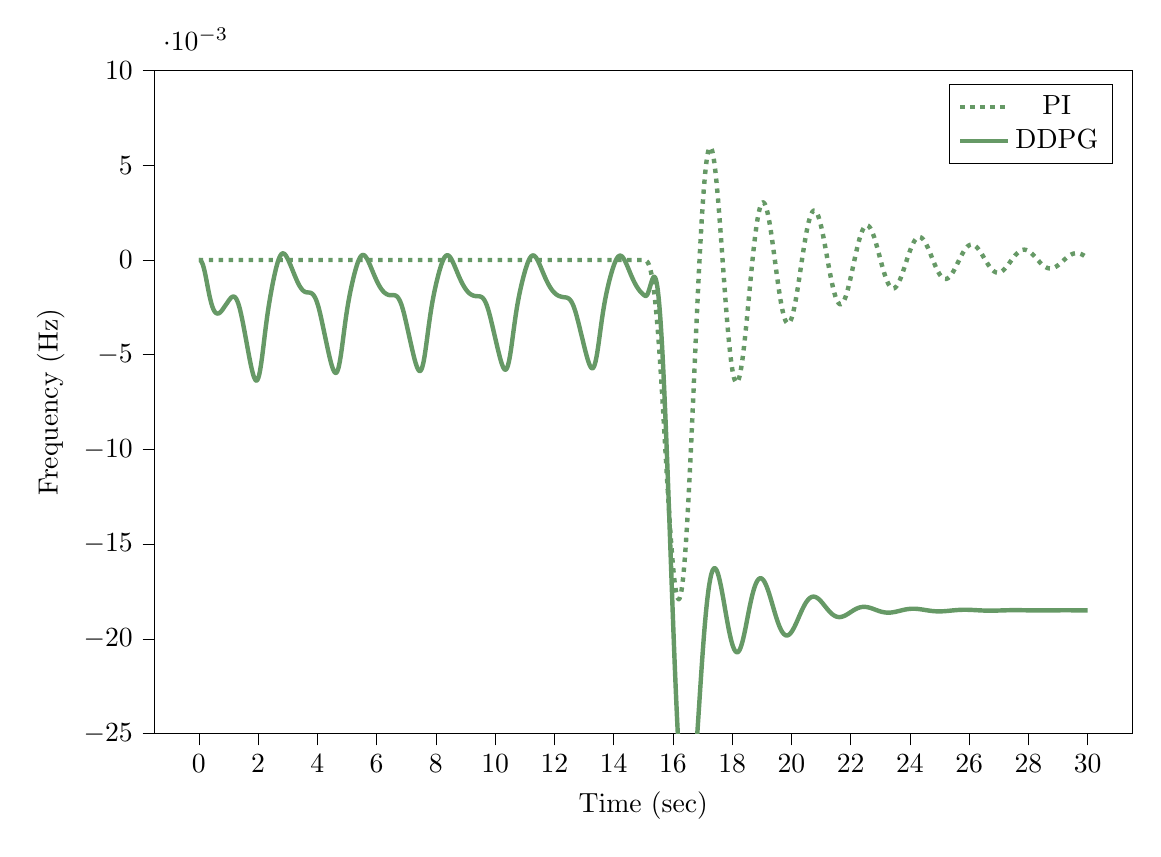
\begin{tikzpicture}

\definecolor{color0}{rgb}{0.12156862745098,0.466666666666667,0.705882352941177}
\definecolor{color1}{rgb}{1,0.498039215686275,0.0549019607843137}

\begin{axis}[
compat=newest,
tick align=outside,
tick pos=left,
x grid style={white!69.0196078431373!black},
xmin=-1.50000000000009, xmax=31.500000000002,
xtick style={color=black},
y grid style={white!69.0196078431373!black},
ymin=-0.025, ymax=0.01,
ytick style={color=black},
%yticklabel style={
%        /pgf/number format/.cd,
%        	fixed,
%        	fixed zerofill,
%         	precision=3,
%        /tikz/.cd
%},
scaled y ticks=true,
scaled y ticks=base 10:3,
width=14cm,
height=10cm,
xlabel=Time (sec),
ylabel=Frequency (Hz)
%y label style={at={(-0.2,0.5)}}
]

\addplot [ultra thick, green!20!gray, dotted]
table {%
0 0
0.01 0
0.02 0
0.03 0
0.04 0
0.05 0
0.06 0
0.07 0
0.08 0
0.09 0
0.1 0
0.11 0
0.12 0
0.13 0
0.14 0
0.15 0
0.16 0
0.17 0
0.18 0
0.19 0
0.2 0
0.21 0
0.22 0
0.23 0
0.24 0
0.25 0
0.26 0
0.27 0
0.28 0
0.29 0
0.3 0
0.31 0
0.32 0
0.33 0
0.34 0
0.35 0
0.36 0
0.37 0
0.38 0
0.39 0
0.4 0
0.41 0
0.42 0
0.43 0
0.44 0
0.45 0
0.46 0
0.47 0
0.48 0
0.49 0
0.5 0
0.51 0
0.52 0
0.53 0
0.54 0
0.55 0
0.56 0
0.57 0
0.58 0
0.59 0
0.6 0
0.61 0
0.62 0
0.63 0
0.64 0
0.65 0
0.66 0
0.67 0
0.68 0
0.69 0
0.7 0
0.71 0
0.72 0
0.73 0
0.74 0
0.75 0
0.76 0
0.77 0
0.78 0
0.79 0
0.8 0
0.81 0
0.820000000000001 0
0.830000000000001 0
0.840000000000001 0
0.850000000000001 0
0.860000000000001 0
0.870000000000001 0
0.880000000000001 0
0.890000000000001 0
0.900000000000001 0
0.910000000000001 0
0.920000000000001 0
0.930000000000001 0
0.940000000000001 0
0.950000000000001 0
0.960000000000001 0
0.970000000000001 0
0.980000000000001 0
0.990000000000001 0
1 0
1.01 0
1.02 0
1.03 0
1.04 0
1.05 0
1.06 0
1.07 0
1.08 0
1.09 0
1.1 0
1.11 0
1.12 0
1.13 0
1.14 0
1.15 0
1.16 0
1.17 0
1.18 0
1.19 0
1.2 0
1.21 0
1.22 0
1.23 0
1.24 0
1.25 0
1.26 0
1.27 0
1.28 0
1.29 0
1.3 0
1.31 0
1.32 0
1.33 0
1.34 0
1.35 0
1.36 0
1.37 0
1.38 0
1.39 0
1.4 0
1.41 0
1.42 0
1.43 0
1.44 0
1.45 0
1.46 0
1.47 0
1.48 0
1.49 0
1.5 0
1.51 0
1.52 0
1.53 0
1.54 0
1.55 0
1.56 0
1.57 0
1.58 0
1.59 0
1.6 0
1.61 0
1.62 0
1.63 0
1.64 0
1.65 0
1.66 0
1.67 0
1.68 0
1.69 0
1.7 0
1.71 0
1.72 0
1.73 0
1.74 0
1.75 0
1.76 0
1.77 0
1.78 0
1.79 0
1.8 0
1.81 0
1.82 0
1.83 0
1.84 0
1.85 0
1.86 0
1.87 0
1.88 0
1.89 0
1.9 0
1.91 0
1.92 0
1.93 0
1.94 0
1.95 0
1.96 0
1.97 0
1.98 0
1.99 0
2 0
2.01 0
2.02 0
2.03 0
2.04 0
2.05 0
2.06 0
2.07 0
2.08 0
2.09 0
2.1 0
2.11 0
2.12 0
2.13 0
2.14 0
2.15 0
2.16 0
2.17 0
2.18 0
2.19 0
2.2 0
2.21 0
2.22 0
2.23 0
2.24 0
2.25 0
2.26 0
2.27 0
2.28 0
2.29 0
2.29999999999999 0
2.30999999999999 0
2.31999999999999 0
2.32999999999999 0
2.33999999999999 0
2.34999999999999 0
2.35999999999999 0
2.36999999999999 0
2.37999999999999 0
2.38999999999999 0
2.39999999999999 0
2.40999999999999 0
2.41999999999999 0
2.42999999999999 0
2.43999999999999 0
2.44999999999999 0
2.45999999999999 0
2.46999999999999 0
2.47999999999999 0
2.48999999999999 0
2.49999999999999 0
2.50999999999999 0
2.51999999999999 0
2.52999999999999 0
2.53999999999999 0
2.54999999999999 0
2.55999999999999 0
2.56999999999999 0
2.57999999999999 0
2.58999999999999 0
2.59999999999999 0
2.60999999999999 0
2.61999999999999 0
2.62999999999999 0
2.63999999999999 0
2.64999999999999 0
2.65999999999999 0
2.66999999999999 0
2.67999999999999 0
2.68999999999999 0
2.69999999999999 0
2.70999999999999 0
2.71999999999999 0
2.72999999999999 0
2.73999999999999 0
2.74999999999999 0
2.75999999999999 0
2.76999999999998 0
2.77999999999998 0
2.78999999999998 0
2.79999999999998 0
2.80999999999998 0
2.81999999999998 0
2.82999999999998 0
2.83999999999998 0
2.84999999999998 0
2.85999999999998 0
2.86999999999998 0
2.87999999999998 0
2.88999999999998 0
2.89999999999998 0
2.90999999999998 0
2.91999999999998 0
2.92999999999998 0
2.93999999999998 0
2.94999999999998 0
2.95999999999998 0
2.96999999999998 0
2.97999999999998 0
2.98999999999998 0
2.99999999999998 0
3.00999999999998 0
3.01999999999998 0
3.02999999999998 0
3.03999999999998 0
3.04999999999998 0
3.05999999999998 0
3.06999999999998 0
3.07999999999998 0
3.08999999999998 0
3.09999999999998 0
3.10999999999998 0
3.11999999999998 0
3.12999999999998 0
3.13999999999998 0
3.14999999999998 0
3.15999999999998 0
3.16999999999998 0
3.17999999999998 0
3.18999999999998 0
3.19999999999998 0
3.20999999999998 0
3.21999999999998 0
3.22999999999998 0
3.23999999999997 0
3.24999999999997 0
3.25999999999997 0
3.26999999999997 0
3.27999999999997 0
3.28999999999997 0
3.29999999999997 0
3.30999999999997 0
3.31999999999997 0
3.32999999999997 0
3.33999999999997 0
3.34999999999997 0
3.35999999999997 0
3.36999999999997 0
3.37999999999997 0
3.38999999999997 0
3.39999999999997 0
3.40999999999997 0
3.41999999999997 0
3.42999999999997 0
3.43999999999997 0
3.44999999999997 0
3.45999999999997 0
3.46999999999997 0
3.47999999999997 0
3.48999999999997 0
3.49999999999997 0
3.50999999999997 0
3.51999999999997 0
3.52999999999997 0
3.53999999999997 0
3.54999999999997 0
3.55999999999997 0
3.56999999999997 0
3.57999999999997 0
3.58999999999997 0
3.59999999999997 0
3.60999999999997 0
3.61999999999997 0
3.62999999999997 0
3.63999999999997 0
3.64999999999997 0
3.65999999999997 0
3.66999999999997 0
3.67999999999997 0
3.68999999999997 0
3.69999999999997 0
3.70999999999996 0
3.71999999999996 0
3.72999999999996 0
3.73999999999996 0
3.74999999999996 0
3.75999999999996 0
3.76999999999996 0
3.77999999999996 0
3.78999999999996 0
3.79999999999996 0
3.80999999999996 0
3.81999999999996 0
3.82999999999996 0
3.83999999999996 0
3.84999999999996 0
3.85999999999996 0
3.86999999999996 0
3.87999999999996 0
3.88999999999996 0
3.89999999999996 0
3.90999999999996 0
3.91999999999996 0
3.92999999999996 0
3.93999999999996 0
3.94999999999996 0
3.95999999999996 0
3.96999999999996 0
3.97999999999996 0
3.98999999999996 0
3.99999999999996 0
4.00999999999996 0
4.01999999999996 0
4.02999999999996 0
4.03999999999996 0
4.04999999999996 0
4.05999999999996 0
4.06999999999996 0
4.07999999999996 0
4.08999999999996 0
4.09999999999996 0
4.10999999999996 0
4.11999999999996 0
4.12999999999996 0
4.13999999999996 0
4.14999999999996 0
4.15999999999996 0
4.16999999999996 0
4.17999999999996 0
4.18999999999996 0
4.19999999999995 0
4.20999999999995 0
4.21999999999995 0
4.22999999999995 0
4.23999999999995 0
4.24999999999995 0
4.25999999999995 0
4.26999999999995 0
4.27999999999995 0
4.28999999999995 0
4.29999999999995 0
4.30999999999995 0
4.31999999999995 0
4.32999999999995 0
4.33999999999995 0
4.34999999999995 0
4.35999999999995 0
4.36999999999995 0
4.37999999999995 0
4.38999999999995 0
4.39999999999995 0
4.40999999999995 0
4.41999999999995 0
4.42999999999995 0
4.43999999999995 0
4.44999999999995 0
4.45999999999995 0
4.46999999999995 0
4.47999999999995 0
4.48999999999995 0
4.49999999999995 0
4.50999999999995 0
4.51999999999995 0
4.52999999999995 0
4.53999999999995 0
4.54999999999995 0
4.55999999999995 0
4.56999999999995 0
4.57999999999995 0
4.58999999999995 0
4.59999999999995 0
4.60999999999995 0
4.61999999999995 0
4.62999999999995 0
4.63999999999995 0
4.64999999999995 0
4.65999999999995 0
4.66999999999994 0
4.67999999999994 0
4.68999999999994 0
4.69999999999994 0
4.70999999999994 0
4.71999999999994 0
4.72999999999994 0
4.73999999999994 0
4.74999999999994 0
4.75999999999994 0
4.76999999999994 0
4.77999999999994 0
4.78999999999994 0
4.79999999999994 0
4.80999999999994 0
4.81999999999994 0
4.82999999999994 0
4.83999999999994 0
4.84999999999994 0
4.85999999999994 0
4.86999999999994 0
4.87999999999994 0
4.88999999999994 0
4.89999999999994 0
4.90999999999994 0
4.91999999999994 0
4.92999999999994 0
4.93999999999994 0
4.94999999999994 0
4.95999999999994 0
4.96999999999994 0
4.97999999999994 0
4.98999999999994 0
4.99999999999994 0
5.00999999999994 0
5.01999999999994 0
5.02999999999994 0
5.03999999999994 0
5.04999999999994 0
5.05999999999994 0
5.06999999999994 0
5.07999999999994 0
5.08999999999994 0
5.09999999999994 0
5.10999999999994 0
5.11999999999994 0
5.12999999999994 0
5.13999999999993 0
5.14999999999993 0
5.15999999999993 0
5.16999999999993 0
5.17999999999993 0
5.18999999999993 0
5.19999999999993 0
5.20999999999993 0
5.21999999999993 0
5.22999999999993 0
5.23999999999993 0
5.24999999999993 0
5.25999999999993 0
5.26999999999993 0
5.27999999999993 0
5.28999999999993 0
5.29999999999993 0
5.30999999999993 0
5.31999999999993 0
5.32999999999993 0
5.33999999999993 0
5.34999999999993 0
5.35999999999993 0
5.36999999999993 0
5.37999999999993 0
5.38999999999993 0
5.39999999999993 0
5.40999999999993 0
5.41999999999993 0
5.42999999999993 0
5.43999999999993 0
5.44999999999993 0
5.45999999999993 0
5.46999999999993 0
5.47999999999993 0
5.48999999999993 0
5.49999999999993 0
5.50999999999993 0
5.51999999999993 0
5.52999999999993 0
5.53999999999993 0
5.54999999999993 0
5.55999999999993 0
5.56999999999993 0
5.57999999999993 0
5.58999999999993 0
5.59999999999993 0
5.60999999999992 0
5.61999999999992 0
5.62999999999992 0
5.63999999999992 0
5.64999999999992 0
5.65999999999992 0
5.66999999999992 0
5.67999999999992 0
5.68999999999992 0
5.69999999999992 0
5.70999999999992 0
5.71999999999992 0
5.72999999999992 0
5.73999999999992 0
5.74999999999992 0
5.75999999999992 0
5.76999999999992 0
5.77999999999992 0
5.78999999999992 0
5.79999999999992 0
5.80999999999992 0
5.81999999999992 0
5.82999999999992 0
5.83999999999992 0
5.84999999999992 0
5.85999999999992 0
5.86999999999992 0
5.87999999999992 0
5.88999999999992 0
5.89999999999992 0
5.90999999999992 0
5.91999999999992 0
5.92999999999992 0
5.93999999999992 0
5.94999999999992 0
5.95999999999992 0
5.96999999999992 0
5.97999999999992 0
5.98999999999992 0
5.99999999999992 0
6.00999999999992 0
6.01999999999992 0
6.02999999999992 0
6.03999999999992 0
6.04999999999992 0
6.05999999999992 0
6.06999999999992 0
6.07999999999991 0
6.08999999999991 0
6.09999999999991 0
6.10999999999991 0
6.11999999999991 0
6.12999999999991 0
6.13999999999991 0
6.14999999999991 0
6.15999999999991 0
6.16999999999991 0
6.17999999999991 0
6.18999999999991 0
6.19999999999991 0
6.20999999999991 0
6.21999999999991 0
6.22999999999991 0
6.23999999999991 0
6.24999999999991 0
6.25999999999991 0
6.26999999999991 0
6.27999999999991 0
6.28999999999991 0
6.29999999999991 0
6.30999999999991 0
6.31999999999991 0
6.32999999999991 0
6.33999999999991 0
6.34999999999991 0
6.35999999999991 0
6.36999999999991 0
6.37999999999991 0
6.38999999999991 0
6.39999999999991 0
6.40999999999991 0
6.41999999999991 0
6.42999999999991 0
6.43999999999991 0
6.44999999999991 0
6.45999999999991 0
6.46999999999991 0
6.47999999999991 0
6.48999999999991 0
6.49999999999991 0
6.50999999999991 0
6.51999999999991 0
6.52999999999991 0
6.53999999999991 0
6.5499999999999 0
6.5599999999999 0
6.5699999999999 0
6.5799999999999 0
6.5899999999999 0
6.5999999999999 0
6.6099999999999 0
6.6199999999999 0
6.6299999999999 0
6.6399999999999 0
6.6499999999999 0
6.6599999999999 0
6.6699999999999 0
6.6799999999999 0
6.6899999999999 0
6.6999999999999 0
6.7099999999999 0
6.7199999999999 0
6.7299999999999 0
6.7399999999999 0
6.7499999999999 0
6.7599999999999 0
6.7699999999999 0
6.7799999999999 0
6.7899999999999 0
6.7999999999999 0
6.8099999999999 0
6.8199999999999 0
6.8299999999999 0
6.8399999999999 0
6.8499999999999 0
6.8599999999999 0
6.8699999999999 0
6.8799999999999 0
6.8899999999999 0
6.8999999999999 0
6.9099999999999 0
6.9199999999999 0
6.9299999999999 0
6.9399999999999 0
6.9499999999999 0
6.9599999999999 0
6.9699999999999 0
6.9799999999999 0
6.9899999999999 0
6.9999999999999 0
7.00999999999989 0
7.01999999999989 0
7.02999999999989 0
7.03999999999989 0
7.04999999999989 0
7.05999999999989 0
7.06999999999989 0
7.07999999999989 0
7.08999999999989 0
7.09999999999989 0
7.10999999999989 0
7.11999999999989 0
7.12999999999989 0
7.13999999999989 0
7.14999999999989 0
7.15999999999989 0
7.16999999999989 0
7.17999999999989 0
7.18999999999989 0
7.19999999999989 0
7.20999999999989 0
7.21999999999989 0
7.22999999999989 0
7.23999999999989 0
7.24999999999989 0
7.25999999999989 0
7.26999999999989 0
7.27999999999989 0
7.28999999999989 0
7.29999999999989 0
7.30999999999989 0
7.31999999999989 0
7.32999999999989 0
7.33999999999989 0
7.34999999999989 0
7.35999999999989 0
7.36999999999989 0
7.37999999999989 0
7.38999999999989 0
7.39999999999989 0
7.40999999999989 0
7.41999999999989 0
7.42999999999989 0
7.43999999999989 0
7.44999999999989 0
7.45999999999989 0
7.46999999999989 0
7.47999999999988 0
7.48999999999988 0
7.49999999999988 0
7.50999999999988 0
7.51999999999988 0
7.52999999999988 0
7.53999999999988 0
7.54999999999988 0
7.55999999999988 0
7.56999999999988 0
7.57999999999988 0
7.58999999999988 0
7.59999999999988 0
7.60999999999988 0
7.61999999999988 0
7.62999999999988 0
7.63999999999988 0
7.64999999999988 0
7.65999999999988 0
7.66999999999988 0
7.67999999999988 0
7.68999999999988 0
7.69999999999988 0
7.70999999999988 0
7.71999999999988 0
7.72999999999988 0
7.73999999999988 0
7.74999999999988 0
7.75999999999988 0
7.76999999999988 0
7.77999999999988 0
7.78999999999988 0
7.79999999999988 0
7.80999999999988 0
7.81999999999988 0
7.82999999999988 0
7.83999999999988 0
7.84999999999988 0
7.85999999999988 0
7.86999999999988 0
7.87999999999988 0
7.88999999999988 0
7.89999999999988 0
7.90999999999988 0
7.91999999999988 0
7.92999999999988 0
7.93999999999988 0
7.94999999999987 0
7.95999999999987 0
7.96999999999987 0
7.97999999999987 0
7.98999999999987 0
7.99999999999987 0
8.00999999999987 0
8.01999999999987 0
8.02999999999987 0
8.03999999999987 0
8.04999999999987 0
8.05999999999987 0
8.06999999999987 0
8.07999999999987 0
8.08999999999987 0
8.09999999999987 0
8.10999999999987 0
8.11999999999987 0
8.12999999999987 0
8.13999999999987 0
8.14999999999987 0
8.15999999999987 0
8.16999999999987 0
8.17999999999987 0
8.18999999999987 0
8.19999999999987 0
8.20999999999987 0
8.21999999999987 0
8.22999999999987 0
8.23999999999987 0
8.24999999999987 0
8.25999999999987 0
8.26999999999987 0
8.27999999999987 0
8.28999999999987 0
8.29999999999987 0
8.30999999999987 0
8.31999999999987 0
8.32999999999987 0
8.33999999999987 0
8.34999999999987 0
8.35999999999987 0
8.36999999999987 0
8.37999999999987 0
8.38999999999987 0
8.39999999999987 0
8.40999999999987 0
8.41999999999986 0
8.42999999999986 0
8.43999999999986 0
8.44999999999986 0
8.45999999999986 0
8.46999999999986 0
8.47999999999986 0
8.48999999999986 0
8.49999999999986 0
8.50999999999986 0
8.51999999999986 0
8.52999999999986 0
8.53999999999986 0
8.54999999999986 0
8.55999999999986 0
8.56999999999986 0
8.57999999999986 0
8.58999999999986 0
8.59999999999986 0
8.60999999999986 0
8.61999999999986 0
8.62999999999986 0
8.63999999999986 0
8.64999999999986 0
8.65999999999986 0
8.66999999999986 0
8.67999999999986 0
8.68999999999986 0
8.69999999999986 0
8.70999999999986 0
8.71999999999986 0
8.72999999999986 0
8.73999999999986 0
8.74999999999986 0
8.75999999999986 0
8.76999999999986 0
8.77999999999986 0
8.78999999999986 0
8.79999999999986 0
8.80999999999986 0
8.81999999999986 0
8.82999999999986 0
8.83999999999986 0
8.84999999999986 0
8.85999999999986 0
8.86999999999986 0
8.87999999999986 0
8.88999999999985 0
8.89999999999985 0
8.90999999999985 0
8.91999999999985 0
8.92999999999985 0
8.93999999999985 0
8.94999999999985 0
8.95999999999985 0
8.96999999999985 0
8.97999999999985 0
8.98999999999985 0
8.99999999999985 0
9.00999999999985 0
9.01999999999985 0
9.02999999999985 0
9.03999999999985 0
9.04999999999985 0
9.05999999999985 0
9.06999999999985 0
9.07999999999985 0
9.08999999999985 0
9.09999999999985 0
9.10999999999985 0
9.11999999999985 0
9.12999999999985 0
9.13999999999985 0
9.14999999999985 0
9.15999999999985 0
9.16999999999985 0
9.17999999999985 0
9.18999999999985 0
9.19999999999985 0
9.20999999999985 0
9.21999999999985 0
9.22999999999985 0
9.23999999999985 0
9.24999999999985 0
9.25999999999985 0
9.26999999999985 0
9.27999999999985 0
9.28999999999985 0
9.29999999999985 0
9.30999999999985 0
9.31999999999985 0
9.32999999999985 0
9.33999999999985 0
9.34999999999985 0
9.35999999999984 0
9.36999999999984 0
9.37999999999984 0
9.38999999999984 0
9.39999999999984 0
9.40999999999984 0
9.41999999999984 0
9.42999999999984 0
9.43999999999984 0
9.44999999999984 0
9.45999999999984 0
9.46999999999984 0
9.47999999999984 0
9.48999999999984 0
9.49999999999984 0
9.50999999999984 0
9.51999999999984 0
9.52999999999984 0
9.53999999999984 0
9.54999999999984 0
9.55999999999984 0
9.56999999999984 0
9.57999999999984 0
9.58999999999984 0
9.59999999999984 0
9.60999999999984 0
9.61999999999984 0
9.62999999999984 0
9.63999999999984 0
9.64999999999984 0
9.65999999999984 0
9.66999999999984 0
9.67999999999984 0
9.68999999999984 0
9.69999999999984 0
9.70999999999984 0
9.71999999999984 0
9.72999999999984 0
9.73999999999984 0
9.74999999999984 0
9.75999999999984 0
9.76999999999984 0
9.77999999999984 0
9.78999999999984 0
9.79999999999984 0
9.80999999999984 0
9.81999999999984 0
9.82999999999983 0
9.83999999999983 0
9.84999999999983 0
9.85999999999983 0
9.86999999999983 0
9.87999999999983 0
9.88999999999983 0
9.89999999999983 0
9.90999999999983 0
9.91999999999983 0
9.92999999999983 0
9.93999999999983 0
9.94999999999983 0
9.95999999999983 0
9.96999999999983 0
9.97999999999983 0
9.98999999999983 0
9.99999999999983 0
10.0099999999998 0
10.0199999999998 0
10.0299999999998 0
10.0399999999998 0
10.0499999999998 0
10.0599999999998 0
10.0699999999998 0
10.0799999999998 0
10.0899999999998 0
10.0999999999998 0
10.1099999999998 0
10.1199999999998 0
10.1299999999998 0
10.1399999999998 0
10.1499999999998 0
10.1599999999998 0
10.1699999999998 0
10.1799999999998 0
10.1899999999998 0
10.1999999999998 0
10.2099999999998 0
10.2199999999998 0
10.2299999999998 0
10.2399999999998 0
10.2499999999998 0
10.2599999999998 0
10.2699999999998 0
10.2799999999998 0
10.2899999999998 0
10.2999999999998 0
10.3099999999998 0
10.3199999999998 0
10.3299999999998 0
10.3399999999998 0
10.3499999999998 0
10.3599999999998 0
10.3699999999998 0
10.3799999999998 0
10.3899999999998 0
10.3999999999998 0
10.4099999999998 0
10.4199999999998 0
10.4299999999998 0
10.4399999999998 0
10.4499999999998 0
10.4599999999998 0
10.4699999999998 0
10.4799999999998 0
10.4899999999998 0
10.4999999999998 0
10.5099999999998 0
10.5199999999998 0
10.5299999999998 0
10.5399999999998 0
10.5499999999998 0
10.5599999999998 0
10.5699999999998 0
10.5799999999998 0
10.5899999999998 0
10.5999999999998 0
10.6099999999998 0
10.6199999999998 0
10.6299999999998 0
10.6399999999998 0
10.6499999999998 0
10.6599999999998 0
10.6699999999998 0
10.6799999999998 0
10.6899999999998 0
10.6999999999998 0
10.7099999999998 0
10.7199999999998 0
10.7299999999998 0
10.7399999999998 0
10.7499999999998 0
10.7599999999998 0
10.7699999999998 0
10.7799999999998 0
10.7899999999998 0
10.7999999999998 0
10.8099999999998 0
10.8199999999998 0
10.8299999999998 0
10.8399999999998 0
10.8499999999998 0
10.8599999999998 0
10.8699999999998 0
10.8799999999998 0
10.8899999999998 0
10.8999999999998 0
10.9099999999998 0
10.9199999999998 0
10.9299999999998 0
10.9399999999998 0
10.9499999999998 0
10.9599999999998 0
10.9699999999998 0
10.9799999999998 0
10.9899999999998 0
10.9999999999998 0
11.0099999999998 0
11.0199999999998 0
11.0299999999998 0
11.0399999999998 0
11.0499999999998 0
11.0599999999998 0
11.0699999999998 0
11.0799999999998 0
11.0899999999998 0
11.0999999999998 0
11.1099999999998 0
11.1199999999998 0
11.1299999999998 0
11.1399999999998 0
11.1499999999998 0
11.1599999999998 0
11.1699999999998 0
11.1799999999998 0
11.1899999999998 0
11.1999999999998 0
11.2099999999998 0
11.2199999999998 0
11.2299999999998 0
11.2399999999998 0
11.2499999999998 0
11.2599999999998 0
11.2699999999998 0
11.2799999999998 0
11.2899999999998 0
11.2999999999998 0
11.3099999999998 0
11.3199999999998 0
11.3299999999998 0
11.3399999999998 0
11.3499999999998 0
11.3599999999998 0
11.3699999999998 0
11.3799999999998 0
11.3899999999998 0
11.3999999999998 0
11.4099999999998 0
11.4199999999998 0
11.4299999999998 0
11.4399999999998 0
11.4499999999998 0
11.4599999999998 0
11.4699999999998 0
11.4799999999998 0
11.4899999999998 0
11.4999999999998 0
11.5099999999998 0
11.5199999999998 0
11.5299999999998 0
11.5399999999998 0
11.5499999999998 0
11.5599999999998 0
11.5699999999998 0
11.5799999999998 0
11.5899999999998 0
11.5999999999998 0
11.6099999999998 0
11.6199999999998 0
11.6299999999998 0
11.6399999999998 0
11.6499999999998 0
11.6599999999998 0
11.6699999999998 0
11.6799999999998 0
11.6899999999998 0
11.6999999999998 0
11.7099999999998 0
11.7199999999998 0
11.7299999999998 0
11.7399999999998 0
11.7499999999998 0
11.7599999999998 0
11.7699999999998 0
11.7799999999998 0
11.7899999999998 0
11.7999999999998 0
11.8099999999998 0
11.8199999999998 0
11.8299999999998 0
11.8399999999998 0
11.8499999999998 0
11.8599999999998 0
11.8699999999998 0
11.8799999999998 0
11.8899999999998 0
11.8999999999998 0
11.9099999999998 0
11.9199999999998 0
11.9299999999998 0
11.9399999999998 0
11.9499999999998 0
11.9599999999998 0
11.9699999999998 0
11.9799999999998 0
11.9899999999998 0
11.9999999999998 0
12.0099999999998 0
12.0199999999998 0
12.0299999999998 0
12.0399999999998 0
12.0499999999998 0
12.0599999999998 0
12.0699999999998 0
12.0799999999998 0
12.0899999999998 0
12.0999999999998 0
12.1099999999998 0
12.1199999999998 0
12.1299999999998 0
12.1399999999998 0
12.1499999999998 0
12.1599999999998 0
12.1699999999998 0
12.1799999999998 0
12.1899999999998 0
12.1999999999998 0
12.2099999999998 0
12.2199999999998 0
12.2299999999998 0
12.2399999999998 0
12.2499999999998 0
12.2599999999998 0
12.2699999999998 0
12.2799999999998 0
12.2899999999998 0
12.2999999999998 0
12.3099999999998 0
12.3199999999998 0
12.3299999999998 0
12.3399999999998 0
12.3499999999998 0
12.3599999999998 0
12.3699999999998 0
12.3799999999998 0
12.3899999999998 0
12.3999999999998 0
12.4099999999998 0
12.4199999999998 0
12.4299999999998 0
12.4399999999998 0
12.4499999999998 0
12.4599999999998 0
12.4699999999998 0
12.4799999999998 0
12.4899999999998 0
12.4999999999998 0
12.5099999999998 0
12.5199999999998 0
12.5299999999998 0
12.5399999999998 0
12.5499999999998 0
12.5599999999998 0
12.5699999999998 0
12.5799999999998 0
12.5899999999998 0
12.5999999999998 0
12.6099999999998 0
12.6199999999998 0
12.6299999999998 0
12.6399999999998 0
12.6499999999998 0
12.6599999999998 0
12.6699999999998 0
12.6799999999998 0
12.6899999999998 0
12.6999999999998 0
12.7099999999998 0
12.7199999999998 0
12.7299999999998 0
12.7399999999998 0
12.7499999999998 0
12.7599999999998 0
12.7699999999998 0
12.7799999999998 0
12.7899999999998 0
12.7999999999998 0
12.8099999999998 0
12.8199999999998 0
12.8299999999998 0
12.8399999999998 0
12.8499999999998 0
12.8599999999998 0
12.8699999999998 0
12.8799999999998 0
12.8899999999998 0
12.8999999999998 0
12.9099999999998 0
12.9199999999998 0
12.9299999999998 0
12.9399999999998 0
12.9499999999998 0
12.9599999999998 0
12.9699999999998 0
12.9799999999998 0
12.9899999999998 0
12.9999999999998 0
13.0099999999998 0
13.0199999999998 0
13.0299999999998 0
13.0399999999998 0
13.0499999999998 0
13.0599999999998 0
13.0699999999998 0
13.0799999999998 0
13.0899999999998 0
13.0999999999998 0
13.1099999999998 0
13.1199999999998 0
13.1299999999998 0
13.1399999999998 0
13.1499999999998 0
13.1599999999998 0
13.1699999999998 0
13.1799999999998 0
13.1899999999998 0
13.1999999999998 0
13.2099999999998 0
13.2199999999998 0
13.2299999999998 0
13.2399999999998 0
13.2499999999998 0
13.2599999999998 0
13.2699999999998 0
13.2799999999998 0
13.2899999999998 0
13.2999999999998 0
13.3099999999998 0
13.3199999999998 0
13.3299999999998 0
13.3399999999998 0
13.3499999999998 0
13.3599999999998 0
13.3699999999998 0
13.3799999999998 0
13.3899999999998 0
13.3999999999998 0
13.4099999999998 0
13.4199999999998 0
13.4299999999998 0
13.4399999999998 0
13.4499999999998 0
13.4599999999998 0
13.4699999999998 0
13.4799999999998 0
13.4899999999998 0
13.4999999999998 0
13.5099999999998 0
13.5199999999998 0
13.5299999999998 0
13.5399999999998 0
13.5499999999998 0
13.5599999999998 0
13.5699999999998 0
13.5799999999998 0
13.5899999999998 0
13.5999999999998 0
13.6099999999998 0
13.6199999999998 0
13.6299999999998 0
13.6399999999998 0
13.6499999999998 0
13.6599999999998 0
13.6699999999998 0
13.6799999999998 0
13.6899999999998 0
13.6999999999998 0
13.7099999999998 0
13.7199999999998 0
13.7299999999998 0
13.7399999999998 0
13.7499999999998 0
13.7599999999998 0
13.7699999999998 0
13.7799999999998 0
13.7899999999998 0
13.7999999999998 0
13.8099999999998 0
13.8199999999997 0
13.8299999999997 0
13.8399999999997 0
13.8499999999997 0
13.8599999999997 0
13.8699999999997 0
13.8799999999997 0
13.8899999999997 0
13.8999999999997 0
13.9099999999997 0
13.9199999999997 0
13.9299999999997 0
13.9399999999997 0
13.9499999999997 0
13.9599999999997 0
13.9699999999997 0
13.9799999999997 0
13.9899999999997 0
13.9999999999997 0
14.0099999999997 0
14.0199999999997 0
14.0299999999997 0
14.0399999999997 0
14.0499999999997 0
14.0599999999997 0
14.0699999999997 0
14.0799999999997 0
14.0899999999997 0
14.0999999999997 0
14.1099999999997 0
14.1199999999997 0
14.1299999999997 0
14.1399999999997 0
14.1499999999997 0
14.1599999999997 0
14.1699999999997 0
14.1799999999997 0
14.1899999999997 0
14.1999999999997 0
14.2099999999997 0
14.2199999999997 0
14.2299999999997 0
14.2399999999997 0
14.2499999999997 0
14.2599999999997 0
14.2699999999997 0
14.2799999999997 0
14.2899999999997 0
14.2999999999997 0
14.3099999999997 0
14.3199999999997 0
14.3299999999997 0
14.3399999999997 0
14.3499999999997 0
14.3599999999997 0
14.3699999999997 0
14.3799999999997 0
14.3899999999997 0
14.3999999999997 0
14.4099999999997 0
14.4199999999997 0
14.4299999999997 0
14.4399999999997 0
14.4499999999997 0
14.4599999999997 0
14.4699999999997 0
14.4799999999997 0
14.4899999999997 0
14.4999999999997 0
14.5099999999997 0
14.5199999999997 0
14.5299999999997 0
14.5399999999997 0
14.5499999999997 0
14.5599999999997 0
14.5699999999997 0
14.5799999999997 0
14.5899999999997 0
14.5999999999997 0
14.6099999999997 0
14.6199999999997 0
14.6299999999997 0
14.6399999999997 0
14.6499999999997 0
14.6599999999997 0
14.6699999999997 0
14.6799999999997 0
14.6899999999997 0
14.6999999999997 0
14.7099999999997 0
14.7199999999997 0
14.7299999999997 0
14.7399999999997 0
14.7499999999997 0
14.7599999999997 0
14.7699999999997 0
14.7799999999997 0
14.7899999999997 0
14.7999999999997 0
14.8099999999997 0
14.8199999999997 0
14.8299999999997 0
14.8399999999997 0
14.8499999999997 0
14.8599999999997 0
14.8699999999997 0
14.8799999999997 0
14.8899999999997 0
14.8999999999997 0
14.9099999999997 0
14.9199999999997 0
14.9299999999997 0
14.9399999999997 0
14.9499999999997 0
14.9599999999997 0
14.9699999999997 0
14.9799999999997 0
14.9899999999997 0
14.9999999999997 0
15.0099999999997 -3.76887919239209e-08
15.0199999999997 -3.03517343632078e-07
15.0299999999997 -1.02150594840761e-06
15.0399999999997 -2.41671580733628e-06
15.0499999999997 -4.71325262026971e-06
15.0599999999997 -8.13414868751079e-06
15.0699999999997 -1.29010205420429e-05
15.0799999999997 -1.9233786077982e-05
15.0899999999997 -2.73503524630568e-05
15.0999999999997 -3.74662777115196e-05
15.1099999999997 -4.97944248201566e-05
15.1199999999997 -6.45446105885083e-05
15.1299999999997 -8.19232507278756e-05
15.1399999999997 -0.000102133003005093
15.1499999999997 -0.000125372410123993
15.1599999999997 -0.000151835543943033
15.1699999999997 -0.000181711652506712
15.1799999999997 -0.00021518481124701
15.1899999999997 -0.000252433579596242
15.1999999999997 -0.000293630664146631
15.2099999999997 -0.000338942589394033
15.2199999999997 -0.00038852937701454
15.2299999999997 -0.000442544234541415
15.2399999999997 -0.000501133254235217
15.2499999999997 -0.000564435122872792
15.2599999999997 -0.000632580843117066
15.2699999999997 -0.000705693467072848
15.2799999999997 -0.000783887842579942
15.2899999999997 -0.000867270372744691
15.2999999999997 -0.000955938789165259
15.3099999999997 -0.00104998193926135
15.3199999999997 -0.00114947958807794
15.3299999999997 -0.00125450223489389
15.3399999999997 -0.0013651109449285
15.3499999999997 -0.00148135719640323
15.3599999999997 -0.00160328274318265
15.3699999999997 -0.00173091949318456
15.3799999999997 -0.00186428940271894
15.3899999999997 -0.0020034043868831
15.3999999999997 -0.00214826624611239
15.4099999999997 -0.00229886660895589
15.4199999999997 -0.00245518689111839
15.4299999999997 -0.00261719827078391
15.4399999999997 -0.00278486167974852
15.4499999999997 -0.00295812781211635
15.4599999999997 -0.00313693714795757
15.4699999999997 -0.00332121999329934
15.4799999999997 -0.00351089653612082
15.4899999999997 -0.00370587691781718
15.4999999999997 -0.00390606132162798
15.5099999999997 -0.00411134007519199
15.5199999999997 -0.004321593768846
15.5299999999997 -0.00453669338898014
15.5399999999997 -0.00475650046620236
15.5499999999997 -0.00498086723804505
15.5599999999997 -0.00520963682592755
15.5699999999997 -0.00544264342606613
15.5799999999997 -0.00567971251368474
15.5899999999997 -0.00592066105844236
15.5999999999997 -0.00616529765656
15.6099999999997 -0.00641342287920812
15.6199999999997 -0.00666482963181566
15.6299999999997 -0.00691930331452614
15.6399999999997 -0.00717662210091017
15.6499999999997 -0.00743655722755908
15.6599999999997 -0.0076988732941092
15.6699999999997 -0.00796332857323173
15.6799999999997 -0.00822967533011167
15.6899999999997 -0.00849766015092534
15.6999999999997 -0.00876702426936767
15.7099999999997 -0.00903750391554902
15.7199999999997 -0.0093088306528098
15.7299999999997 -0.00958073186163605
15.7399999999997 -0.00985293100635227
15.7499999999997 -0.01012514800758
15.7599999999997 -0.0103970996200657
15.7699999999997 -0.0106684998153339
15.7799999999997 -0.0109390601688078
15.7899999999997 -0.011208490250282
15.7999999999997 -0.0114764980177068
15.8099999999997 -0.0117427902129511
15.8199999999997 -0.0120070727603425
15.8299999999997 -0.0122690511691175
15.8399999999997 -0.0125284309323785
15.8499999999997 -0.0127849179283431
15.8599999999997 -0.0130382188213927
15.8699999999997 -0.0132880414623653
15.8799999999997 -0.0135340952875374
15.8899999999997 -0.0137760917157415
15.8999999999997 -0.0140137445430766
15.9099999999997 -0.0142467703346646
15.9199999999997 -0.0144748888129219
15.9299999999997 -0.0146978232412412
15.9399999999997 -0.0149153008026934
15.9499999999997 -0.0151270529783358
15.9599999999997 -0.0153328159142644
15.9699999999997 -0.0155323307846532
15.9799999999997 -0.0157253441482461
15.9899999999997 -0.0159116082978225
15.9999999999997 -0.016090881602171
16.0099999999997 -0.0162629288401107
16.0199999999997 -0.0164275215261182
16.0299999999997 -0.0165844382271243
16.0399999999997 -0.0167334648700591
16.0499999999997 -0.0168743950397348
16.0599999999997 -0.0170070302672907
16.0699999999997 -0.0171311809894126
16.0799999999997 -0.0172466654963271
16.0899999999997 -0.0173533108261179
16.0999999999997 -0.0174509530095695
16.1099999999997 -0.017539437303271
16.1199999999997 -0.0176186184106906
16.1299999999997 -0.0176883606909478
16.1399999999997 -0.0177485383550268
16.1499999999997 -0.0177990356491939
16.1599999999997 -0.0178397470253946
16.1699999999997 -0.0178705772984288
16.1799999999997 -0.0178914417897164
16.1899999999997 -0.0179022664574856
16.1999999999997 -0.017902988013234
16.2099999999997 -0.0178935540243307
16.2199999999997 -0.0178739230026472
16.2299999999997 -0.0178440644791209
16.2399999999997 -0.0178039590641772
16.2499999999997 -0.0177535984939521
16.2599999999997 -0.0176929856622763
16.2699999999997 -0.0176221346384026
16.2799999999997 -0.0175410706704734
16.2899999999997 -0.0174498301747466
16.2999999999997 -0.0173484607106148
16.3099999999998 -0.0172370209414722
16.3199999999998 -0.0171155806792989
16.3299999999998 -0.0169842208778355
16.3399999999998 -0.0168430331535691
16.3499999999998 -0.0166921199313693
16.3599999999998 -0.0165315944641963
16.3699999999998 -0.0163615806583916
16.3799999999998 -0.0161822126482664
16.3899999999998 -0.0159936348640597
16.3999999999998 -0.0157960018709324
16.4099999999998 -0.0155894781954378
16.4199999999998 -0.0153742381406455
16.4299999999998 -0.0151504655912628
16.4399999999998 -0.0149183537952739
16.4499999999998 -0.0146781051470304
16.4599999999998 -0.0144299309546976
16.4699999999998 -0.0141740511967914
16.4799999999998 -0.0139106942766218
16.4899999999998 -0.0136400967534338
16.4999999999998 -0.0133625030513367
16.5099999999998 -0.0130781651886886
16.5199999999998 -0.0127873424853093
16.5299999999998 -0.0124903019308347
16.5399999999998 -0.012187316681878
16.5499999999998 -0.0118786659600469
16.5599999999998 -0.0115646350478153
16.5699999999998 -0.0112455149530464
16.5799999999998 -0.0109216020674296
16.5899999999998 -0.0105931978191455
16.5999999999998 -0.0102606083201018
16.6099999999998 -0.0099241440081264
16.6199999999998 -0.00958411928451374
16.6299999999998 -0.009240852147354
16.6399999999998 -0.00889466382107602
16.6499999999998 -0.00854587839287554
16.6599999999998 -0.00819482241491342
16.6699999999998 -0.00784182453554155
16.6799999999998 -0.00748721511892218
16.6899999999998 -0.00713132586248777
16.6999999999998 -0.0067744894133937
16.7099999999998 -0.00641703898444042
16.7199999999998 -0.00605930796993765
16.7299999999998 -0.00570162956198807
16.7399999999998 -0.00534433636766493
16.7499999999998 -0.0049877600275538
16.7599999999998 -0.00463223083613038
16.7699999999998 -0.00427807736444114
16.7799999999998 -0.00392562608554654
16.7899999999998 -0.00357520100317634
16.7999999999998 -0.00322712328396608
16.8099999999998 -0.00288171089408463
16.8199999999998 -0.00253927824029083
16.8299999999998 -0.00220013581594263
16.8399999999998 -0.00186458985243158
16.8499999999998 -0.0015329419764631
16.8599999999998 -0.00120548887359007
16.8699999999998 -0.000882521958401192
16.8799999999998 -0.00056432705175512
16.8899999999998 -0.000251184065440229
16.8999999999998 5.66333053666735e-05
16.9099999999998 0.000358857881483448
16.9199999999998 0.000655229290593409
16.9299999999998 0.000945494249311422
16.9399999999998 0.00122940683604183
16.9499999999999 0.00150672875437251
16.9599999999999 0.00177722958664312
16.9699999999999 0.00204068703738106
16.9799999999999 0.00229688716663334
16.9899999999999 0.00254562461259706
16.9999999999999 0.00278670280340085
17.0099999999999 0.00301993415781625
17.0199999999999 0.00324514027468377
17.0299999999999 0.0034621521108513
17.0399999999999 0.00367081014743823
17.0499999999999 0.00387096454425546
17.0599999999999 0.00406247528222369
17.0699999999999 0.0042452122936493
17.0799999999999 0.00441905558023284
17.0899999999999 0.00458389531869965
17.0999999999999 0.00473963195285958
17.1099999999999 0.00488617626758871
17.1199999999999 0.00502344947392897
17.1299999999999 0.00515138325561441
17.1399999999999 0.00526991981102394
17.1499999999999 0.00537901188309061
17.1599999999999 0.00547862277648051
17.1699999999999 0.00556872636222763
17.1799999999999 0.00564930707015588
17.1899999999999 0.00572035986603779
17.1999999999999 0.00578189021909391
17.2099999999999 0.00583391488226037
17.2199999999999 0.00587646026732258
17.2299999999999 0.00590956309293109
17.2399999999999 0.00593327032931215
17.2499999999999 0.00594763910451941
17.2599999999999 0.00595273659887214
17.2699999999999 0.00594863992775189
17.2799999999999 0.00593543601154246
17.2899999999999 0.00591322143637474
17.2999999999999 0.00588210230792785
17.3099999999999 0.00584219408546131
17.3199999999999 0.00579362140948507
17.3299999999999 0.00573651791909434
17.3399999999999 0.00567102605923187
17.3499999999999 0.00559729687815015
17.3599999999999 0.00551548981541002
17.3699999999999 0.00542577248067734
17.3799999999999 0.00532832042329264
17.3899999999999 0.00522331689362095
17.3999999999999 0.00511095259600212
17.4099999999999 0.00499142543376723
17.4199999999999 0.00486494024666638
17.4299999999999 0.0047317085410625
17.4399999999999 0.00459194821325415
17.4499999999999 0.00444588326630039
17.4599999999999 0.00429374352072686
17.4699999999999 0.00413576431950509
17.4799999999999 0.00397218622770386
17.4899999999999 0.00380325473968125
17.4999999999999 0.00362921996084573
17.5099999999999 0.00345033627034573
17.5199999999999 0.00326686202275841
17.5299999999999 0.00307905922747289
17.5399999999999 0.00288719402361346
17.5499999999999 0.00269153629577341
17.5599999999999 0.00249235650106056
17.5699999999999 0.00228992752068486
17.5799999999999 0.00208452430386135
17.59 0.0018764235177507
17.6 0.00166590320144227
17.61 0.00145324242290304
17.62 0.00123872093835087
17.63 0.00102261885383134
17.64 0.000805216288981428
17.65 0.000586793043092566
17.66 0.000367628263662495
17.67 0.00014800011768668
17.68 -7.1814534028563e-05
17.69 -0.000291540459224935
17.7 -0.000510904372901807
17.71 -0.000729635252051716
17.72 -0.000947464646082432
17.73 -0.00116412698259394
17.74 -0.00137935986817529
17.75 -0.00159290438389324
17.76 -0.00180450537514451
17.77 -0.00201391173555396
17.78 -0.00222087668460391
17.79 -0.00242515803868873
17.8 -0.00262651847529682
17.81 -0.00282472579003197
17.82 -0.00301955314619204
17.83 -0.00321077931601069
17.84 -0.00339818891510054
17.85 -0.00358157262871615
17.86 -0.0037607274284684
17.87 -0.0039354567808487
17.88 -0.00410557084684938
17.89 -0.00427088667247469
17.9 -0.00443122836994943
17.91 -0.00458642728944511
17.92 -0.00473632218115491
17.93 -0.00488075934756051
17.94 -0.00501959278574734
17.95 -0.00515268431963747
17.96 -0.00527990372202043
17.97 -0.0054011288262767
17.98 -0.00551624562769924
17.99 -0.00562514837433254
18 -0.00572773964725885
18.01 -0.00582393043027624
18.02 -0.00591364016892007
18.03 -0.00599679681879555
18.04 -0.006073336883195
18.05 -0.00614320543998473
18.06 -0.00620635669691625
18.07 -0.00626275328332388
18.08 -0.00631236611480636
18.09 -0.00635517468707673
18.1 -0.00639116705084892
18.11 -0.00642033977635476
18.12 -0.00644269790758766
18.13 -0.00645825490638043
18.14 -0.00646703258643725
18.15 -0.00646906103745087
18.16 -0.00646437853944792
18.17 -0.00645303146751624
18.18 -0.00643507418707947
18.19 -0.00641056893692624
18.2 -0.00637958571139762
18.21 -0.00634220212815289
18.22 -0.00629850328541302
18.2300000000001 -0.00624858161272188
18.2400000000001 -0.00619253671362849
18.2500000000001 -0.00613047520032861
18.2600000000001 -0.00606251052053785
18.2700000000001 -0.0059887627768582
18.2800000000001 -0.00590935853889982
18.2900000000001 -0.00582443064842885
18.3000000000001 -0.0057341180211062
18.3100000000001 -0.00563856543468676
18.3200000000001 -0.00553792331431405
18.3300000000001 -0.00543234751326306
18.3400000000001 -0.00532199908764573
18.3500000000001 -0.0052070440658961
18.3600000000001 -0.0050876532133676
18.3700000000001 -0.0049640017923788
18.3800000000001 -0.00483627059128321
18.3900000000001 -0.0047046434092125
18.4000000000001 -0.00456930727588844
18.4100000000001 -0.00443045273778487
18.4200000000001 -0.00428827359531919
18.4300000000001 -0.004142966638326
18.4400000000001 -0.00399473137992814
18.4500000000001 -0.0038437697889802
18.4600000000001 -0.00369028602130648
18.4700000000001 -0.00353448614998433
18.4800000000001 -0.00337657789494557
18.4900000000001 -0.00321677035218485
18.5000000000001 -0.0030552737228977
18.5100000000001 -0.0028922990427872
18.5200000000001 -0.00272805791186412
18.5300000000001 -0.00256276222519397
18.5400000000001 -0.00239662390474586
18.5500000000001 -0.00222985463271231
18.5600000000001 -0.00206266558661686
18.5700000000001 -0.00189526717652073
18.5800000000001 -0.0017278687846405
18.5900000000001 -0.00156067850768352
18.6000000000001 -0.00139390290220457
18.6100000000001 -0.00122774673328317
18.6200000000001 -0.00106241272681467
18.6300000000001 -0.000898101325705174
18.6400000000001 -0.000735010450251106
18.6500000000001 -0.000573335262982784
18.6600000000001 -0.000413267938239868
18.6700000000001 -0.000254997436743212
18.6800000000001 -9.87092854178155e-05
18.6900000000001 5.54146372830429e-05
18.7000000000001 0.000207196310312436
18.7100000000001 0.000356461772991858
18.7200000000001 0.000503041321781714
18.7300000000001 0.000646769700632151
18.7400000000001 0.000787486284716786
18.7500000000001 0.000925035257351725
18.7600000000001 0.00105926578646706
18.7700000000001 0.00119003223531147
18.7800000000001 0.00131719421110805
18.7900000000001 0.00144061676507192
18.8000000000001 0.00156017053272362
18.8100000000001 0.00167573186640586
18.8200000000001 0.00178718295987555
18.8300000000001 0.00189441196485392
18.8400000000001 0.00199731309942813
18.8500000000001 0.00209578674782638
18.8600000000001 0.0021897395518563
18.8700000000002 0.00227908449613224
18.8800000000002 0.00236374098198284
18.8900000000002 0.00244363489386265
18.9000000000002 0.00251869865718723
18.9100000000002 0.0025888712875539
18.9200000000002 0.00265409843132059
18.9300000000002 0.00271433239752178
18.9400000000002 0.00276953236056118
18.9500000000002 0.00281966458026665
18.9600000000002 0.00286470150922735
18.9700000000002 0.00290462230700344
18.9800000000002 0.00293941282984779
18.9900000000002 0.00296906561196087
19.0000000000002 0.00299357983838606
19.0100000000002 0.003012961309612
19.0200000000002 0.0030272223979705
19.0300000000002 0.00303638199592821
19.0400000000002 0.0030404654563798
19.0500000000002 0.00303950452505978
19.0600000000002 0.00303353726519941
19.0700000000002 0.00302260797456395
19.0800000000002 0.00300676711230002
19.0900000000002 0.00298607121433646
19.1000000000002 0.00296058271010292
19.1100000000002 0.00293036985848709
19.1200000000002 0.00289550662767859
19.1300000000002 0.00285607257152954
19.1400000000002 0.00281215269979109
19.1500000000002 0.00276383733779195
19.1600000000002 0.0027112219824176
19.1700000000002 0.00265440715227832
19.1800000000002 0.00259349823228794
19.1900000000002 0.00252860531288264
19.2000000000002 0.00245984302540205
19.2100000000002 0.00238733037152808
19.2200000000002 0.00231119054458724
19.2300000000002 0.00223155075082106
19.2400000000002 0.00214854202565142
19.2500000000002 0.0020622990460185
19.2600000000002 0.00197295993910381
19.2700000000002 0.00188066608774288
19.2800000000002 0.00178556309631641
19.2900000000002 0.00168779899643512
19.3000000000002 0.00158752336393155
19.3100000000002 0.00148488826621718
19.3200000000002 0.00138004804279044
19.3300000000002 0.00127315908691788
19.3400000000002 0.00116437962787016
19.3500000000002 0.00105386951339552
19.3600000000002 0.000941789992304579
19.3700000000002 0.000828303497162081
19.3800000000002 0.000713573427163915
19.3900000000002 0.000597763931331052
19.4000000000002 0.000481039692190006
19.4100000000002 0.000363565710134814
19.4200000000002 0.000245507088681932
19.4300000000002 0.000127028820842673
19.4400000000002 8.29557684421042e-06
19.4500000000002 -0.000110528506564482
19.4600000000002 -0.000229280034982496
19.4700000000002 -0.000347796563163327
19.4800000000002 -0.000465916799518158
19.4900000000002 -0.000583480808077148
19.5000000000002 -0.000700330207676168
19.5100000000003 -0.000816308368134254
19.5200000000003 -0.000931260603192192
19.5300000000003 -0.00104503435998912
19.5400000000003 -0.00115747940485636
19.5500000000003 -0.00126844800521399
19.5600000000003 -0.00137779510735939
19.5700000000003 -0.0014853785099457
19.5800000000003 -0.00159105903295029
19.5900000000003 -0.00169470068194356
19.6000000000003 -0.00179617080747149
19.6100000000003 -0.00189534025937498
19.6200000000003 -0.00199208353587413
19.6300000000003 -0.00208627892725296
19.6400000000003 -0.00217780865398978
19.6500000000003 -0.00226655899918186
19.6600000000003 -0.00235242043512466
19.6700000000003 -0.0024352877439114
19.6800000000003 -0.00251506013192692
19.6900000000003 -0.00259164133811846
19.7000000000003 -0.00266493973593376
19.7100000000003 -0.00273486842882403
19.7200000000003 -0.0028013453392187
19.7300000000003 -0.00286429329088526
19.7400000000003 -0.00292364008459676
19.7500000000003 -0.00297931856703603
19.7600000000003 -0.0030312666928731
19.7700000000003 -0.00307942757995919
19.7800000000003 -0.00312374955758745
19.7900000000003 -0.00316418620777439
19.8000000000003 -0.00320069664948363
19.8100000000003 -0.00323324564383654
19.8200000000003 -0.00326180276652212
19.8300000000003 -0.00328634294512547
19.8400000000003 -0.00330684646641523
19.8500000000003 -0.0033232989767229
19.8600000000003 -0.00333569147545991
19.8700000000003 -0.003344020301807
19.8800000000003 -0.00334828711462737
19.8900000000003 -0.0033484988656636
19.9000000000003 -0.00334466776608581
19.9100000000003 -0.00333681124646699
19.9200000000003 -0.00332495191026874
19.9300000000003 -0.00330911748092887
19.9400000000003 -0.00328934074264965
19.9500000000003 -0.00326565947499291
19.9600000000003 -0.0032381163813962
19.9700000000003 -0.00320675901173094
19.9800000000003 -0.00317163967673703
19.9900000000003 -0.00313281536353005
20.0000000000003 -0.00309034763967301
20.0100000000003 -0.00304430255246829
20.0200000000003 -0.00299475052367398
20.0300000000003 -0.00294176623928464
20.0400000000003 -0.00288542853433854
20.0500000000003 -0.00282582027297447
20.0600000000003 -0.00276302822391449
20.0700000000003 -0.00269714293154755
20.0800000000003 -0.00262825858383086
20.0900000000003 -0.00255647287634641
20.1000000000003 -0.00248188686594389
20.1100000000003 -0.00240460482921206
20.1200000000003 -0.00232473411468372
20.1300000000003 -0.00224238499184868
20.1400000000003 -0.00215767049722766
20.1500000000004 -0.00207070627775619
20.1600000000004 -0.00198161043174066
20.1700000000004 -0.00189050432871836
20.1800000000004 -0.0017975112660488
20.1900000000004 -0.00170275533667033
20.2000000000004 -0.00160636248754581
20.2100000000004 -0.00150846030297914
20.2200000000004 -0.00140917781466335
20.2300000000004 -0.00130864535272067
20.2400000000004 -0.00120699436716582
20.2500000000004 -0.00110435725006289
20.2600000000004 -0.00100086715824725
20.2700000000004 -0.000896657836586853
20.2800000000004 -0.000791863441831836
20.2900000000004 -0.00068661836714589
20.3000000000004 -0.000581057067445889
20.3100000000004 -0.00047531388569956
20.3200000000004 -0.000369522880344038
20.3300000000004 -0.000263817654000667
20.3400000000004 -0.000158331183666346
20.3500000000004 -5.31956525671612e-05
20.3600000000004 5.14577161394735e-05
20.3700000000004 0.000155498823624403
20.3800000000004 0.000258798857420697
20.3900000000004 0.000361230451048625
20.4000000000004 0.000462667841043625
20.4100000000004 0.000562987021205649
20.4200000000004 0.000662065893894029
20.4300000000004 0.000759784418190895
20.4400000000004 0.000856024754762983
20.4500000000004 0.000950671407255313
20.4600000000004 0.001043611360055
20.4700000000004 0.0011347342122675
20.4800000000004 0.00122393230775433
20.4900000000004 0.00131110086108532
20.5000000000004 0.00139613807926433
20.5100000000004 0.00147894527909365
20.5200000000004 0.00155942700004764
20.5300000000004 0.0016374911125319
20.5400000000004 0.00171304892141225
20.5500000000004 0.00178601526470067
20.5600000000004 0.00185630860729599
20.5700000000004 0.00192385112967975
20.5800000000004 0.00198856881147657
20.5900000000004 0.0020503915097938
20.6000000000004 0.00210925303226228
20.6100000000004 0.0021650912047059
20.6200000000004 0.00221784793337469
20.6300000000004 0.00226746926168261
20.6400000000004 0.00231390542139567
20.6500000000004 0.00235711087822467
20.6600000000004 0.00239704437177927
20.6700000000004 0.00243366894984733
20.6800000000004 0.00246695199696598
20.6900000000004 0.00249686525725507
20.7000000000004 0.00252338545705216
20.7100000000004 0.00254649340165739
20.7200000000004 0.00256617405013822
20.7300000000004 0.00258241675991955
20.7400000000004 0.00259521528210453
20.7500000000004 0.00260456775121853
20.7600000000004 0.00261047666940916
20.7700000000004 0.00261294888514996
20.7800000000004 0.00261199556650129
20.7900000000005 0.00260763216898885
20.8000000000005 0.00259987839816632
20.8100000000005 0.00258875816693501
20.8200000000005 0.00257429954769943
20.8300000000005 0.00255653471944417
20.8400000000005 0.00253549990982286
20.8500000000005 0.00251123533235652
20.8600000000005 0.00248378511884392
20.8700000000005 0.00245319724709226
20.8800000000005 0.00241952346408232
20.8900000000005 0.00238281920401243
20.9000000000005 0.00234314350333444
20.9100000000005 0.00230055891229262
20.9200000000005 0.00225513139975678
20.9300000000005 0.00220693025546501
20.9400000000005 0.00215602798849476
20.9500000000005 0.00210250022211161
20.9600000000005 0.00204642558590371
20.9700000000005 0.00198788560391019
20.9800000000005 0.00192696457706335
20.9900000000005 0.00186374946658051
21.0000000000005 0.00179832977320653
21.0100000000005 0.00173079741380061
21.0200000000005 0.00166124659547773
21.0300000000005 0.0015897736875109
21.0400000000005 0.00151647709120665
21.0500000000005 0.00144145735161984
21.0600000000005 0.00136481828945121
21.0700000000005 0.00128666317522398
21.0800000000005 0.00120709682350444
21.0900000000005 0.00112622543998834
21.1000000000005 0.00104415647120967
21.1100000000005 0.00096099845590138
21.1200000000005 0.000876860877435977
21.1300000000005 0.000791854017021655
21.1400000000005 0.000706088807488476
21.1500000000005 0.000619676687603666
21.1600000000005 0.000532729456922714
21.1700000000005 0.000445359131231777
21.1800000000005 0.000357677798667405
21.1900000000005 0.000269797476623547
21.2000000000005 0.000181829969569756
21.2100000000005 9.38867279169832e-05
21.2200000000005 6.07870807182779e-06
21.2300000000005 -8.1483766171849e-05
21.2400000000005 -0.000168691140749966
21.2500000000005 -0.000255434766809518
21.2600000000005 -0.000341607034397448
21.2700000000005 -0.000427101504206279
21.2800000000005 -0.000511813037228124
21.2900000000005 -0.00059563792216521
21.3000000000005 -0.000678474000453128
21.3100000000005 -0.000760220788752131
21.3200000000005 -0.000840779598766659
21.3300000000005 -0.000920053654255562
21.3400000000005 -0.00099794820510004
21.3500000000005 -0.00107437063829885
21.3600000000005 -0.0011492305857659
21.3700000000005 -0.00122244002880868
21.3800000000005 -0.00129391339892307
21.3900000000005 -0.00136356767537552
21.4000000000005 -0.0014313224795322
21.4100000000005 -0.00149710016460963
21.4200000000005 -0.00156082590189641
21.4300000000006 -0.00162242776302544
21.4400000000006 -0.00168183679820833
21.4500000000006 -0.00173898711034969
21.4600000000006 -0.00179381592496373
21.4700000000006 -0.00184626365582031
21.4800000000006 -0.00189627396625313
21.4900000000006 -0.00194379382606781
21.5000000000006 -0.00198877356399159
21.5100000000006 -0.00203116691561218
21.5200000000006 -0.00207093106675631
21.5300000000006 -0.0021080266922634
21.5400000000006 -0.00214241799011236
21.5500000000006 -0.0021740727108618
21.5600000000006 -0.00220296220707043
21.5700000000006 -0.00222906203119774
21.5800000000006 -0.00225235101922228
21.5900000000006 -0.00227281139488619
21.6000000000006 -0.00229042901615536
21.6100000000006 -0.00230519337750177
21.6200000000006 -0.00231709760756991
21.6300000000006 -0.00232613846224915
21.6400000000006 -0.00233231631318052
21.6500000000006 -0.00233563513173553
21.6600000000006 -0.00233610246850925
21.6700000000006 -0.00233372942837568
21.6800000000006 -0.0023285306411581
21.6900000000006 -0.0023205242279727
21.7000000000006 -0.00230973176330844
21.7100000000006 -0.00229617823291154
21.7200000000006 -0.00227989198754753
21.7300000000006 -0.00226090469271919
21.7400000000006 -0.00223925127442294
21.7500000000006 -0.00221496986103179
21.7600000000006 -0.00218810172139767
21.7700000000006 -0.00215869119929168
21.7800000000006 -0.00212678564286516
21.7900000000006 -0.00209243533470093
21.8000000000006 -0.00205569341974824
21.8100000000006 -0.00201661582357523
21.8200000000006 -0.00197526115912052
21.8300000000006 -0.00193169064920267
21.8400000000006 -0.0018859680385447
21.8500000000006 -0.00183815950253246
21.8600000000006 -0.00178833355264022
21.8700000000006 -0.00173656094068601
21.8800000000006 -0.00168291456034101
21.8900000000006 -0.00162746934639973
21.9000000000006 -0.00157030217198324
21.9100000000006 -0.00151149174384254
21.9200000000006 -0.00145111849592958
21.9300000000006 -0.00138926448141069
21.9400000000006 -0.00132601524624538
21.9500000000006 -0.00126145559186877
21.9600000000006 -0.0011956713598988
21.9700000000006 -0.00112874961089598
21.9800000000006 -0.00106077849692676
21.9900000000006 -0.000991847136602969
22.0000000000006 -0.000922045491746211
22.0100000000006 -0.000851464245165655
22.0200000000006 -0.000780194679251402
22.0300000000006 -0.000708328555224983
22.0400000000006 -0.000635957992977222
22.0500000000006 -0.000563175351485877
22.0600000000006 -0.000490073109847067
22.0700000000007 -0.000416743748982475
22.0800000000007 -0.000343279634105168
22.0900000000007 -0.000269772898040536
22.1000000000007 -0.000196315325508395
22.1100000000007 -0.000122998238479019
22.1200000000007 -4.99123827212404e-05
22.1300000000007 2.2852184338789e-05
22.1400000000007 9.52062043250067e-05
22.1500000000007 0.000167061327064067
22.1600000000007 0.000238330218062151
22.1700000000007 0.00030892666418298
22.1800000000007 0.000378765677409579
22.1900000000007 0.000447763596571037
22.2000000000007 0.000515838186919939
22.2100000000007 0.000582908737446469
22.2200000000007 0.000648896155819844
22.2300000000007 0.000713723060849592
22.2400000000007 0.000777313872362855
22.2500000000007 0.000839594898396777
22.2600000000007 0.000900494419609075
22.2700000000007 0.000959942770813151
22.2800000000007 0.00101787241947531
22.2900000000007 0.00107421804089649
22.3000000000007 0.00112891659143315
22.3100000000007 0.00118190737725244
22.3200000000007 0.00123313212022302
22.3300000000007 0.00128253502045218
22.3400000000007 0.00133006281540332
22.3500000000007 0.00137566483553273
22.3600000000007 0.00141929305638861
22.3700000000007 0.00146090214711906
22.3800000000007 0.00150044951534006
22.3900000000007 0.00153789534831813
22.4000000000007 0.00157320265042618
22.4100000000007 0.00160633727683367
22.4200000000007 0.00163726796339614
22.4300000000007 0.00166596635271026
22.4400000000007 0.00169240701630289
22.4500000000007 0.00171656747292235
22.4600000000007 0.00173842880579259
22.4700000000007 0.00175797479741125
22.4800000000007 0.00177519194005787
22.4900000000007 0.00179006971255393
22.5000000000007 0.00180260058027067
22.5100000000007 0.00181277999135662
22.5200000000007 0.00182060636920209
22.5300000000007 0.00182608110116976
22.5400000000007 0.00182920852362517
22.5500000000007 0.00182999590330471
22.5600000000007 0.00182845341506319
22.5700000000007 0.00182459411604717
22.5800000000007 0.00181843391634422
22.5900000000007 0.00180999154616261
22.6000000000007 0.00179928851959986
22.6100000000007 0.0017863490950625
22.6200000000007 0.00177120023240352
22.6300000000007 0.00175387154684796
22.6400000000007 0.00173439525978088
22.6500000000007 0.00171280614647668
22.6600000000007 0.00168914148087232
22.6700000000007 0.00166344097668688
22.6800000000007 0.00163574672759703
22.6900000000007 0.00160610314355368
22.7000000000007 0.00157455688403815
22.7100000000008 0.00154115678924712
22.7200000000008 0.00150595380885904
22.7300000000008 0.00146900092865094
22.7400000000008 0.00143035309440446
22.7500000000008 0.0013900671340666
22.7600000000008 0.00134820167798486
22.7700000000008 0.00130481707723448
22.7800000000008 0.00125997532018685
22.7900000000008 0.00121373994745255
22.8000000000008 0.00116617596527257
22.8100000000008 0.00111734975591593
22.8200000000008 0.00106732898870491
22.8300000000008 0.00101618484505719
22.8400000000008 0.000963986886933686
22.8500000000008 0.000910805690509283
22.8600000000008 0.000856712803686117
22.8700000000008 0.000801780636993911
22.8800000000008 0.000746082358778858
22.8900000000008 0.000689691792344826
22.9000000000008 0.000632683314459732
22.9100000000008 0.000575131754873395
22.9200000000008 0.000517112296638869
22.9300000000008 0.000458700377128751
22.9400000000008 0.000399971589702386
22.9500000000008 0.000341001586023616
22.9600000000008 0.000281865979061066
22.9700000000008 0.000222640246822385
22.9800000000008 0.000163399636890713
22.9900000000008 0.000104219071840501
23.0000000000008 4.51730556183535e-05
23.0100000000008 -1.36644190206163e-05
23.0200000000008 -7.22199619279228e-05
23.0300000000008 -0.000130420875732715
23.0400000000008 -0.000188195244672747
23.0500000000008 -0.000245472021987415
23.0600000000008 -0.000302181115778107
23.0700000000008 -0.000358253473239598
23.0800000000008 -0.00041362116316919
23.0900000000008 -0.000468217456660979
23.1000000000008 -0.000521976905895135
23.1100000000008 -0.000574835420933592
23.1200000000008 -0.000626730344437037
23.1300000000008 -0.000677600524219308
23.1400000000008 -0.000727386383558967
23.1500000000008 -0.000776029989190477
23.1600000000008 -0.000823475116900299
23.1700000000008 -0.000869667314310993
23.1800000000008 -0.000914553962027775
23.1900000000008 -0.000958084331512258
23.2000000000008 -0.00100020964032596
23.2100000000008 -0.00104088310473895
23.2200000000008 -0.00108005998956131
23.2300000000008 -0.001117697655146
23.2400000000008 -0.00115375560151407
23.2500000000008 -0.00118819550955648
23.2600000000008 -0.00122098127927077
23.2700000000008 -0.00125207906499265
23.2800000000008 -0.00128145730758624
23.2900000000008 -0.00130908676355905
23.3000000000008 -0.00133494053106945
23.3100000000008 -0.00135899407279699
23.3200000000008 -0.00138122523564562
23.3300000000008 -0.00140161426725078
23.3400000000008 -0.00142014411560331
23.3500000000009 -0.00143680049080612
23.3600000000009 -0.00145157096916294
23.3700000000009 -0.00146444556629985
23.3800000000009 -0.00147541673880157
23.3900000000009 -0.00148447938274401
23.4000000000009 -0.00149163082913237
23.4100000000009 -0.00149687083626773
23.4200000000009 -0.00150020157906868
23.4300000000009 -0.00150162763537764
23.4400000000009 -0.00150115596928517
23.4500000000009 -0.00149879591150872
23.4600000000009 -0.00149455913686571
23.4700000000009 -0.00148845963888427
23.4800000000009 -0.00148051370159787
23.4900000000009 -0.00147073986857403
23.5000000000009 -0.00145915890922962
23.5100000000009 -0.00144579378248926
23.5200000000009 -0.00143066959784593
23.5300000000009 -0.00141381357388613
23.5400000000009 -0.00139525499435018
23.5500000000009 -0.00137502516179688
23.5600000000009 -0.0013531573486964
23.5700000000009 -0.00132968674681092
23.5800000000009 -0.00130465041413854
23.5900000000009 -0.00127808721950182
23.6000000000009 -0.00125003778530107
23.6100000000009 -0.00122054442834846
23.6200000000009 -0.00118965109881143
23.6300000000009 -0.00115740331742122
23.6400000000009 -0.0011238481108446
23.6500000000009 -0.00108903394505373
23.6600000000009 -0.00105301065823661
23.6700000000009 -0.00101582939187156
23.6800000000009 -0.000977542520448052
23.6900000000009 -0.000938203579971014
23.7000000000009 -0.000897867195332597
23.7100000000009 -0.000856590607171173
23.7200000000009 -0.000814430893104607
23.7300000000009 -0.000771445081284174
23.7400000000009 -0.000727691046347975
23.7500000000009 -0.000683227418045026
23.7600000000009 -0.000638113493199392
23.7700000000009 -0.000592409150551098
23.7800000000009 -0.000546174766260788
23.7900000000009 -0.000499471130009843
23.8000000000009 -0.000452359362816157
23.8100000000009 -0.000404900835533476
23.8200000000009 -0.00035715708795774
23.8300000000009 -0.000309189748512712
23.8400000000009 -0.000261060454518426
23.8500000000009 -0.000212830773070855
23.8600000000009 -0.000164562122575576
23.8700000000009 -0.000116315694732468
23.8800000000009 -6.8152377114457e-05
23.8900000000009 -2.01326778856761e-05
23.9000000000009 2.76833494737026e-05
23.9100000000009 7.52361804240341e-05
23.9200000000009 0.000122466892552472
23.9300000000009 0.000169317237612038
23.9400000000009 0.000215729712336271
23.9500000000009 0.00026164762795209
23.9600000000009 0.000307015178314717
23.9700000000009 0.000351777506589993
23.9800000000009 0.000395880770409717
23.990000000001 0.000439272205427377
24.000000000001 0.000481900187203866
24.010000000001 0.000523714291354718
24.020000000001 0.000564665351891607
24.030000000001 0.00060470551769452
24.040000000001 0.000643788307051796
24.050000000001 0.000681868660067664
24.060000000001 0.000718902989209841
24.070000000001 0.000754849227994282
24.080000000001 0.000789666877033351
24.090000000001 0.000823317048071646
24.100000000001 0.000855762505770156
24.110000000001 0.000886967707194619
24.120000000001 0.000916898838966453
24.130000000001 0.000945523852037379
24.140000000001 0.000972812494051306
24.150000000001 0.000998736339259113
24.160000000001 0.00102326881595457
24.170000000001 0.00104638523140109
24.180000000001 0.00106806279422096
24.190000000001 0.00108828063421946
24.200000000001 0.00110701981961673
24.210000000001 0.00112426337165988
24.220000000001 0.00113999637203957
24.230000000001 0.00115420657464046
24.240000000001 0.0011668829796722
24.250000000001 0.00117801657670058
24.260000000001 0.00118760034722108
24.270000000001 0.00119562926467571
24.280000000001 0.00120210029193072
24.290000000001 0.00120701237623106
24.300000000001 0.00121036644165252
24.310000000001 0.00121216537907516
24.320000000001 0.00121241403370419
24.330000000001 0.00121111919016747
24.340000000001 0.00120828955522104
24.350000000001 0.00120393573809733
24.360000000001 0.00119807022853282
24.370000000001 0.00119070737251505
24.380000000001 0.00118186334579109
24.390000000001 0.00117155612518252
24.400000000001 0.0011598054577542
24.410000000001 0.00114663282788681
24.420000000001 0.00113206142230551
24.430000000001 0.00111611609313192
24.440000000001 0.00109882331897505
24.450000000001 0.00108021116413971
24.460000000001 0.00106030923583664
24.470000000001 0.00103914863995521
24.480000000001 0.00101676193507066
24.490000000001 0.000993183084798253
24.500000000001 0.00096844740859802
24.510000000001 0.000942591531100315
24.520000000001 0.00091565333184764
24.530000000001 0.000887671889338551
24.540000000001 0.000858687426042111
24.550000000001 0.000828741253567895
24.560000000001 0.000797875715680156
24.570000000001 0.000766134130258796
24.580000000001 0.000733560730264252
24.590000000001 0.000700201050700501
24.600000000001 0.000666102952043566
24.610000000001 0.000631312590755228
24.620000000001 0.000595876865305747
24.6300000000011 0.000559843335698812
24.6400000000011 0.000523260147512367
24.6500000000011 0.000486175958930396
24.6600000000011 0.000448639871070609
24.6700000000011 0.000410701356271608
24.6800000000011 0.000372410189292835
24.6900000000011 0.000333816381322859
24.7000000000011 0.000294970113022568
24.7100000000011 0.000255921668364755
24.7200000000011 0.000216721368886648
24.7300000000011 0.00017741950817387
24.7400000000011 0.000138066287274205
24.7500000000011 9.87117507178291e-05
24.7600000000011 5.94057231796892e-05
24.7700000000011 2.01977468318901e-05
24.7800000000011 -1.88629805615738e-05
24.7900000000011 -5.77276667503312e-05
24.8000000000011 -9.63479852452793e-05
24.8100000000011 -0.000134676134646846
24.8200000000011 -0.000172664896992936
24.8300000000011 -0.000210267695064469
24.8400000000011 -0.000247438648587081
24.8500000000011 -0.000284132629267923
24.8600000000011 -0.000320305314607061
24.8700000000011 -0.00035591324042472
24.8800000000011 -0.000390913852045874
24.8900000000011 -0.000425265554085973
24.9000000000011 -0.000458927758782878
24.9100000000011 -0.000491860932821689
24.9200000000011 -0.000524026642600718
24.9300000000011 -0.000555387597837933
24.9400000000011 -0.000585907693431233
24.9500000000011 -0.000615552050164276
24.9600000000011 -0.000644287053051748
24.9700000000011 -0.000672080388107789
24.9800000000011 -0.000698901077288646
24.9900000000011 -0.000724719511571621
25.0000000000011 -0.000749507482135477
25.0100000000011 -0.000773238209608894
25.0200000000011 -0.000795886371355418
25.0300000000011 -0.000817428126765777
25.0400000000011 -0.000837841140529194
25.0500000000011 -0.00085710460385743
25.0600000000011 -0.000875199253636109
25.0700000000011 -0.000892107389478266
25.0800000000011 -0.000907812888655471
25.0900000000011 -0.000922301218870923
25.1000000000011 -0.000935559448812521
25.1100000000011 -0.000947576943095906
25.1200000000011 -0.000958344237663811
25.1300000000011 -0.000967853308370546
25.1400000000011 -0.000976097757838802
25.1500000000011 -0.000983072816424456
25.1600000000011 -0.000988775341096052
25.1700000000011 -0.000993203812239449
25.1800000000011 -0.000996358328404537
25.1900000000011 -0.000998240599013106
25.2000000000011 -0.000998853935048919
25.2100000000011 -0.000998203237753223
25.2200000000011 -0.000996294985351009
25.2300000000011 -0.000993137217835508
25.2400000000011 -0.000988739519840491
25.2500000000011 -0.000983113001632107
25.2600000000011 -0.000976270278254032
25.2700000000012 -0.000968225446861809
25.2800000000012 -0.000958994062284293
25.2900000000012 -0.000948593110852113
25.3000000000012 -0.000937040982535026
25.3100000000012 -0.00092435744143449
25.3200000000012 -0.000910563594677043
25.3300000000012 -0.000895681859732991
25.3400000000012 -0.000879735930252945
25.3500000000012 -0.000862750740442188
25.3600000000012 -0.000844752428033152
25.3700000000012 -0.000825768295909496
25.3800000000012 -0.000805826772436951
25.3900000000012 -0.000784957370556994
25.4000000000012 -0.000763190645700171
25.4100000000012 -0.000740558152576134
25.4200000000012 -0.000717092400897411
25.4300000000012 -0.000692826810092141
25.4400000000012 -0.000667795663058726
25.4500000000012 -0.000642034318316953
25.4600000000012 -0.000615578459644762
25.4700000000012 -0.000588464691405316
25.4800000000012 -0.000560732063542175
25.4900000000012 -0.000532418695554385
25.5000000000012 -0.000503562438058232
25.5100000000012 -0.000474202197370932
25.5200000000012 -0.000444377099467727
25.5300000000012 -0.000414126722529466
25.5400000000012 -0.00038349103661342
25.5500000000012 -0.000352510345115324
25.5600000000012 -0.000321225227522898
25.5700000000012 -0.000289676483140613
25.5800000000012 -0.000257905075581584
25.5900000000012 -0.000225952077900232
25.6000000000012 -0.000193858618293024
25.6100000000012 -0.000161665826329883
25.6200000000012 -0.000129414779705464
25.6300000000012 -9.71464515170801e-05
25.6400000000012 -6.49016580891396e-05
25.6500000000012 -3.27210073734451e-05
25.6600000000012 -6.44847961062494e-07
25.6700000000012 3.12867812533905e-05
25.6800000000012 6.30342007110708e-05
25.6900000000012 9.45581390837725e-05
25.7000000000012 0.00012581978135421
25.7100000000012 0.000156780816119272
25.7200000000012 0.000187403481978283
25.7300000000012 0.000217650612970061
25.7400000000012 0.000247485683024932
25.7500000000012 0.000276872849383967
25.7600000000012 0.000305776994937861
25.7700000000012 0.000334163769439228
25.7800000000012 0.000361999629543285
25.7900000000012 0.000389251877632715
25.8000000000012 0.000415888699384447
25.8100000000012 0.000441879200037248
25.8200000000012 0.000467193439145669
25.8300000000012 0.000491802464398863
25.8400000000012 0.000515678343722638
25.8500000000012 0.000538794195915314
25.8600000000012 0.00056112421985744
25.8700000000012 0.000582643722222131
25.8800000000012 0.000603329143617268
25.8900000000012 0.000623158083158353
25.9000000000012 0.000642109321449231
25.9100000000013 0.000660162841938611
25.9200000000013 0.000677299850627842
25.9300000000013 0.00069350279410673
25.9400000000013 0.000708755375894375
25.9500000000013 0.000723042571062546
25.9600000000013 0.000736350639118564
25.9700000000013 0.000748667135123778
25.9800000000013 0.000759980919021115
25.9900000000013 0.000770282408041691
26.0000000000013 0.00077956374914362
26.0100000000013 0.000787817817140062
26.0200000000013 0.00079503881569491
26.0300000000013 0.000801222278918104
26.0400000000013 0.000806365071242147
26.0500000000013 0.000810465385590668
26.0600000000013 0.000813522739852544
26.0700000000013 0.000815537971677274
26.0800000000013 0.000816513231608765
26.0900000000013 0.000816451974576422
26.1000000000013 0.000815358949763988
26.1100000000013 0.000813240188878284
26.1200000000013 0.000810102992841643
26.1300000000013 0.000805955916933536
26.1400000000013 0.000800808754408542
26.1500000000013 0.000794672518619443
26.1600000000013 0.000787559423675876
26.1700000000013 0.000779482863670635
26.1800000000013 0.000770457390507132
26.1900000000013 0.000760498690363287
26.2000000000013 0.000749623558835459
26.2100000000013 0.000737849874775881
26.2200000000013 0.000725196572892732
26.2300000000013 0.000711683615141304
26.2400000000013 0.000697331960946459
26.2500000000013 0.000682163536301064
26.2600000000013 0.000666201201784017
26.2700000000013 0.000649468719542522
26.2800000000013 0.000631990883522262
26.2900000000013 0.000613793031389892
26.3000000000013 0.000594901429209764
26.3100000000013 0.000575343104561299
26.3200000000013 0.000555145809470228
26.3300000000013 0.000534337982719069
26.3400000000013 0.00051294871163046
26.3500000000013 0.000491007693436013
26.3600000000013 0.000468545951604739
26.3700000000013 0.000445595745653938
26.3800000000013 0.00042218790751137
26.3900000000013 0.000398353776172407
26.4000000000013 0.000374125140367509
26.4100000000013 0.000349534185121112
26.4200000000013 0.000324613440938105
26.4300000000013 0.000299395579347551
26.4400000000013 0.000273913878950542
26.4500000000013 0.000248201609893822
26.4600000000013 0.000222292199810902
26.4700000000013 0.000196219188191433
26.4800000000013 0.000170016181349733
26.4900000000013 0.0001437168079243
26.5000000000013 0.000117354674871638
26.5100000000013 9.09633239396754e-05
26.5200000000013 6.45761886219783e-05
26.5300000000013 3.82265516051523e-05
26.5400000000013 1.19475027299404e-05
26.5500000000014 -1.42281025071276e-05
26.5600000000014 -4.02676838808663e-05
26.5700000000014 -6.61389767593038e-05
26.5800000000014 -9.1810071784535e-05
26.5900000000014 -0.000117249453874572
26.6000000000014 -0.000142426040508556
26.6100000000014 -0.000167309219255979
26.6200000000014 -0.000191868884511706
26.6300000000014 -0.000216075473397844
26.6400000000014 -0.000239900000794338
26.6500000000014 -0.000263314093460901
26.6600000000014 -0.00028629002321333
26.6700000000014 -0.000308800739118239
26.6800000000014 -0.000330819898671341
26.6900000000014 -0.000352321897925442
26.7000000000014 -0.000373281900488998
26.7100000000014 -0.000393675865398428
26.7200000000014 -0.000413480574135685
26.7300000000014 -0.00043267365611248
26.7400000000014 -0.000451233613079404
26.7500000000014 -0.000469139842306462
26.7600000000014 -0.000486372658509866
26.7700000000014 -0.000502913314500708
26.7800000000014 -0.00051874402053278
26.7900000000014 -0.000533847962327196
26.8000000000014 -0.000548209317752879
26.8100000000014 -0.000561813272142242
26.8200000000014 -0.000574646032222054
26.8300000000014 -0.000586694838639247
26.8400000000014 -0.000597947977061056
26.8500000000014 -0.000608394787827687
26.8600000000014 -0.000618025674133467
26.8700000000014 -0.00062683210870894
26.8800000000014 -0.000634807358806159
26.8900000000014 -0.000641945261993712
26.9000000000014 -0.000648240591317165
26.9100000000014 -0.000653689206553487
26.9200000000014 -0.000658288054793457
26.9300000000014 -0.000662035169616844
26.9400000000014 -0.000664929668870439
26.9500000000014 -0.000666971751062263
26.9600000000014 -0.000668162690386252
26.9700000000014 -0.000668504830392962
26.9800000000014 -0.000668001576323038
26.9900000000014 -0.000666657386121451
27.0000000000014 -0.000664477760151814
27.0100000000014 -0.000661469229631331
27.0200000000014 -0.000657639343808293
27.0300000000014 -0.000652996655905306
27.0400000000014 -0.000647550707852709
27.0500000000014 -0.000641312013837937
27.0600000000014 -0.000634292042697821
27.0700000000014 -0.000626503199182017
27.0800000000014 -0.000617958804119022
27.0900000000014 -0.000608673174461472
27.1000000000014 -0.000598661319999565
27.1100000000014 -0.000587939182762908
27.1200000000014 -0.000576523531573452
27.1300000000014 -0.000564431937272504
27.1400000000014 -0.000551682747069541
27.1500000000014 -0.000538295058054766
27.1600000000014 -0.000524288689919994
27.1700000000014 -0.000509684156935224
27.1800000000014 -0.000494502639231992
27.1900000000015 -0.000478765953449267
27.2000000000015 -0.000462496522804022
27.2100000000015 -0.000445717346657394
27.2200000000015 -0.000428451969659658
27.2300000000015 -0.000410724450575557
27.2400000000015 -0.000392559331545744
27.2500000000015 -0.000373983628817011
27.2600000000015 -0.000355022693431563
27.2700000000015 -0.000335701892607249
27.2800000000015 -0.000316046992070295
27.2900000000015 -0.000296084108793706
27.3000000000015 -0.000275839666911236
27.3100000000015 -0.000255340355813258
27.3200000000015 -0.000234613089784856
27.3300000000015 -0.000213684968768581
27.3400000000015 -0.000192583239976858
27.3500000000015 -0.000171335260173129
27.3600000000015 -0.00014996845850451
27.3700000000015 -0.000128510148678322
27.3800000000015 -0.000106987978598328
27.3900000000015 -8.54293711165313e-05
27.4000000000015 -6.38616779665097e-05
27.4100000000015 -4.23121446096577e-05
27.4200000000015 -2.08078755273903e-05
27.4300000000015 6.24200027570279e-07
27.4400000000015 2.19573618017519e-05
27.4500000000015 4.31651318110999e-05
27.4600000000015 6.42213070848251e-05
27.4700000000015 8.50999918555268e-05
27.4800000000015 0.000105775629166689
27.4900000000015 0.00012622303186773
27.5000000000015 0.000146417412966216
27.5100000000015 0.000166334415306923
27.5200000000015 0.000185950140547126
27.5300000000015 0.000205241177398153
27.5400000000015 0.00022418462910325
27.5500000000015 0.000242758140122713
27.5600000000015 0.000260939921997775
27.5700000000015 0.000278708778365333
27.5800000000015 0.00029604412909668
27.5900000000015 0.000312926033419269
27.6000000000015 0.000329335212402569
27.6100000000015 0.000345253070289315
27.6200000000015 0.000360661714844593
27.6300000000015 0.000375543976741691
27.6400000000015 0.000389883427929524
27.6500000000015 0.000403664398961088
27.6600000000015 0.000416871995263297
27.6700000000015 0.000429492112329265
27.6800000000015 0.00044151144981469
27.6900000000015 0.000452917524520394
27.7000000000015 0.000463698682243283
27.7100000000015 0.000473844108477742
27.7200000000015 0.000483343837948941
27.7300000000015 0.000492188712184391
27.7400000000015 0.000500370550057015
27.7500000000015 0.000507881980627603
27.7600000000015 0.000514716838134393
27.7700000000015 0.000520870082876665
27.7800000000015 0.000526337040931322
27.7900000000015 0.000531113925486985
27.8000000000015 0.000535197837841
27.8100000000015 0.000538586767244941
27.8200000000015 0.000541279589605863
27.8300000000016 0.000543276065053411
27.8400000000016 0.000544576834383988
27.8500000000016 0.000545183414394205
27.8600000000016 0.000545098192116872
27.8700000000016 0.00054432441797387
27.8800000000016 0.000542866197861342
27.8900000000016 0.00054072848418377
27.9000000000016 0.000537917065854619
27.9100000000016 0.000534438557282389
27.9200000000016 0.000530300386362038
27.9300000000016 0.000525510781492943
27.9400000000016 0.000520078757645696
27.9500000000016 0.000514014101501211
27.9600000000016 0.000507327355686846
27.9700000000016 0.000500029802139678
27.9800000000016 0.000492133444608911
27.9900000000016 0.00048365099034558
28.0000000000016 0.000474595830999353
28.0100000000016 0.000464982022754676
28.0200000000016 0.000454824265739883
28.0300000000016 0.000444137882744373
28.0400000000016 0.000432938797281107
28.0500000000016 0.00042124351103457
28.0600000000016 0.000409069080737743
28.0700000000016 0.000396433094526174
28.0800000000016 0.000383353647823465
28.0900000000016 0.000369849318820785
28.1000000000016 0.000355939143625132
28.1100000000016 0.000341642591168707
28.1200000000016 0.000326979537997909
28.1300000000016 0.0003119711608738
28.1400000000016 0.000296639323219836
28.1500000000016 0.000281004510894805
28.1600000000016 0.000265087565101429
28.1700000000016 0.000248909639639264
28.1800000000016 0.000232492161973241
28.1900000000016 0.000215856796895524
28.2000000000016 0.000199025411998815
28.2100000000016 0.00018202004445075
28.2200000000016 0.000164862868732129
28.2300000000016 0.000147576165114122
28.2400000000016 0.000130182288724898
28.2500000000016 0.000112703639107054
28.2600000000016 9.51626302028646e-05
28.2700000000016 7.75816607289947e-05
28.2800000000016 5.9983084920311e-05
28.2900000000016 4.23891836351661e-05
28.3000000000016 2.48221358236959e-05
28.3100000000016 7.30399036769761e-06
28.3200000000016 -1.01433616944065e-05
28.3300000000016 -2.74982145404781e-05
28.3400000000016 -4.4739074515591e-05
28.3500000000016 -6.18446866392089e-05
28.3600000000016 -7.87940606455681e-05
28.3700000000016 -9.55664965333595e-05
28.3800000000016 -0.000112141609600117
28.3900000000016 -0.00012849946788397
28.4000000000016 -0.00014462026224524
28.4100000000016 -0.000160484700674475
28.4200000000016 -0.000176073900646476
28.4300000000016 -0.000191369411242892
28.4400000000016 -0.000206353234608097
28.4500000000016 -0.00022100784671618
28.4600000000016 -0.000235316217427261
28.4700000000017 -0.000249261829777173
28.4800000000017 -0.000262828605462433
28.4900000000017 -0.00027600121248116
28.5000000000017 -0.00028876478080198
28.5100000000017 -0.000301105023420499
28.5200000000017 -0.000313008251712747
28.5300000000017 -0.00032446138994753
28.5400000000017 -0.00033545198894103
28.5500000000017 -0.000345968238837545
28.5600000000017 -0.000355998981000878
28.5700000000017 -0.000365533719001213
28.5800000000017 -0.000374562628682553
28.5900000000017 -0.00038307656729583
28.6000000000017 -0.000391067081682352
28.6100000000017 -0.000398526415491514
28.6200000000017 -0.000405447515415323
28.6300000000017 -0.000411824036420089
28.6400000000017 -0.000417650345952434
28.6500000000017 -0.000422922362187418
28.6600000000017 -0.000427635989759381
28.6700000000017 -0.000431787812166251
28.6800000000017 -0.000435375137238303
28.6900000000017 -0.000438395997478202
28.7000000000017 -0.000440849149459547
28.7100000000017 -0.000442734072291629
28.7200000000017 -0.000444050965159865
28.7300000000017 -0.000444800743951982
28.7400000000017 -0.000444985036980907
28.7500000000017 -0.000444606179816088
28.7600000000017 -0.00044366720923585
28.7700000000017 -0.000442171856314256
28.7800000000017 -0.000440124538656848
28.7900000000017 -0.000437530351800552
28.8000000000017 -0.000434395059793961
28.8100000000017 -0.000430725084975156
28.8200000000017 -0.00042652749696521
28.8300000000017 -0.000421810000896449
28.8400000000017 -0.000416580924895619
28.8500000000017 -0.000410849206844463
28.8600000000017 -0.000404624380437105
28.8700000000017 -0.000397916560556251
28.8800000000017 -0.000390736428000557
28.8900000000017 -0.00038309521358256
28.9000000000017 -0.000375004681626504
28.9100000000017 -0.000366477112895478
28.9200000000017 -0.000357525286979338
28.9300000000017 -0.000348162464177584
28.9400000000017 -0.000338402366914683
28.9500000000017 -0.000328259160729819
28.9600000000017 -0.000317747434888884
28.9700000000017 -0.000306882182674789
28.9800000000017 -0.000295678781423848
28.9900000000017 -0.000284152970621285
29.0000000000017 -0.000272320829171001
29.0100000000017 -0.000260198756913183
29.0200000000017 -0.000247805628187784
29.0300000000017 -0.000235158165500965
29.0400000000017 -0.000222273183379261
29.0500000000017 -0.000209167783299157
29.0600000000017 -0.000195859312066713
29.0700000000017 -0.000182365328989987
29.0800000000017 -0.000168703575972986
29.0900000000017 -0.000154891949107667
29.1000000000017 -0.000140948471358452
29.1100000000018 -0.000126891266067958
29.1200000000018 -0.000112738531100969
29.1300000000018 -9.85085135035292e-05
29.1400000000018 -8.42194845949055e-05
29.1500000000018 -6.98897154390197e-05
29.1600000000018 -5.553745266217e-05
29.1700000000018 -4.11808945985248e-05
29.1800000000018 -2.68381677554901e-05
29.1900000000018 -1.25273035988006e-05
29.2000000000018 1.73378433708995e-06
29.2100000000018 1.59273230035054e-05
29.2200000000018 3.00357020439911e-05
29.2300000000018 4.40414956374782e-05
29.2400000000018 5.79274839614152e-05
29.2500000000018 7.16766742566574e-05
29.2600000000018 8.52723214754412e-05
29.2700000000018 9.86979484930245e-05
29.2800000000018 0.000111937365863414
29.2900000000018 0.000124974691099591
29.3000000000018 0.000137794367458512
29.3100000000018 0.000150381182211581
29.3200000000018 0.000162720284381462
29.3300000000018 0.000174797201926508
29.3400000000018 0.000186597858354489
29.3500000000018 0.000198108588747856
29.3600000000018 0.000209316155096261
29.3700000000018 0.000220207761239254
29.3800000000018 0.000230771066982378
29.3900000000018 0.000240994201585496
29.4000000000018 0.000250865776597589
29.4100000000018 0.000260374898007885
29.4200000000018 0.000269511177699256
29.4300000000018 0.000278264744190452
29.4400000000018 0.000286626252653908
29.4500000000018 0.000294586894196314
29.4600000000018 0.000302138404389037
29.4700000000018 0.000309273071035507
29.4800000000018 0.00031598374116221
29.4900000000018 0.000322263827219231
29.5000000000018 0.000328107312474952
29.5100000000018 0.000333508755587634
29.5200000000018 0.000338463294333718
29.5300000000018 0.000342967097901472
29.5400000000018 0.000347016931904257
29.5500000000018 0.00035060974687885
29.5600000000018 0.000353743083501882
29.5700000000018 0.000356415073253664
29.5800000000018 0.000358624438307452
29.5900000000018 0.000360370490650227
29.6000000000018 0.000361653130442895
29.6100000000018 0.000362472843628391
29.6200000000018 0.000362830698796706
29.6300000000018 0.000362728343316525
29.6400000000018 0.000362167998743778
29.6500000000018 0.000361152455518127
29.6600000000018 0.000359685066959089
29.6700000000018 0.000357769742574253
29.6800000000018 0.000355410940692776
29.6900000000018 0.000352613660438144
29.7000000000018 0.000349383433054948
29.7100000000018 0.00034572631260528
29.7200000000018 0.000341648866051182
29.7300000000018 0.00033715816274048
29.7400000000018 0.000332261763316762
29.7500000000019 0.000326967708063645
29.7600000000019 0.00032128450471626
29.7700000000019 0.000315221115754311
29.7800000000019 0.000308786945201126
29.7900000000019 0.000301991824953644
29.8000000000019 0.000294846000670124
29.8100000000019 0.000287360117244997
29.8200000000019 0.000279545203698594
29.8300000000019 0.000271412656613869
29.8400000000019 0.000262974225125121
29.8500000000019 0.000254241995081093
29.8600000000019 0.000245228372754268
29.8700000000019 0.000235946068333244
29.8800000000019 0.000226408079255056
29.8900000000019 0.000216627673448154
29.9000000000019 0.000206619512126296
29.9100000000019 0.000196398362907465
29.9200000000019 0.000185977752333156
29.9300000000019 0.000175371464380501
29.9400000000019 0.000164593506471762
29.9500000000019 0.00015365807961018
29.9600000000019 0.000142579551310659
29.9700000000019 0.000131372431908296
29.9800000000019 0.000120051350161329
29.9900000000019 0.000108631028940748
30.0000000000019 9.71262634946441e-05
};
\addlegendentry{PI};
\addplot [ultra thick, green!20!gray]
table {%
0 0
0.01 -1.48877540917823e-07
0.02 -1.15398358188589e-06
0.03 -3.77979997995336e-06
0.04 -8.69496037508394e-06
0.05 -1.64646028768568e-05
0.06 -2.75573375304501e-05
0.07 -4.23555373994048e-05
0.08 -6.11640491722483e-05
0.09 -8.42132937654195e-05
0.1 -0.000111657834993305
0.11 -0.000143588034685615
0.12 -0.000180037238530438
0.13 -0.000220987025684277
0.14 -0.000266371964892216
0.15 -0.000316083895712395
0.16 -0.000369976950515259
0.17 -0.000427871855094342
0.18 -0.000489558616579765
0.19 -0.000554793719864138
0.2 -0.000623299171028353
0.21 -0.000694765383893376
0.22 -0.000768857352415366
0.23 -0.000845220840587354
0.24 -0.000923488252316593
0.25 -0.00100328402139687
0.26 -0.00108422956745695
0.27 -0.00116594781113971
0.28 -0.00124806723967769
0.29 -0.00133022552687261
0.3 -0.00141207270875716
0.31 -0.00149327392101444
0.32 -0.00157351175712464
0.33 -0.00165248830813083
0.34 -0.00172992682067733
0.35 -0.00180557295403592
0.36 -0.00187919565805709
0.37 -0.0019505877019015
0.38 -0.00201956588760949
0.39 -0.00208597097727096
0.4 -0.00214966736034769
0.41 -0.00221054249609092
0.42 -0.00226850616013739
0.43 -0.00232348952184897
0.44 -0.00237544408161456
0.45 -0.00242434049278494
0.46 -0.00247016728548753
0.47 -0.00251292951373016
0.48 -0.00255264835324375
0.49 -0.00258935795792075
0.5 -0.00262310512377863
0.51 -0.00265394770458817
0.52 -0.00268195335080676
0.53 -0.00270719729618427
0.54 -0.0027297615410848
0.55 -0.00274973241675587
0.56 -0.00276719363658476
0.57 -0.00278222556476932
0.58 -0.00279490603080797
0.59 -0.00280531101755307
0.6 -0.00281351502581938
0.61 -0.00281959035641733
0.62 -0.00282360573946848
0.63 -0.00282562757255204
0.64 -0.00282572088731472
0.65 -0.00282395026011203
0.66 -0.00282038014181254
0.67 -0.00281507466169835
0.68 -0.00280809792322323
0.69 -0.00279951486010095
0.7 -0.00278939202414012
0.71 -0.00277779817702503
0.72 -0.00276480473246406
0.73 -0.00275048615061918
0.74 -0.00273491878350368
0.75 -0.00271818177876729
0.76 -0.00270035806313426
0.77 -0.00268153316031779
0.78 -0.00266179501226585
0.79 -0.00264123510126926
0.8 -0.00261995049670392
0.81 -0.00259804646261284
0.820000000000001 -0.00257563480374583
0.830000000000001 -0.00255283260528808
0.840000000000001 -0.00252975993437179
0.850000000000001 -0.00250653746492795
0.860000000000001 -0.00248328429110315
0.870000000000001 -0.00246011595483807
0.880000000000001 -0.00243714217293164
0.890000000000001 -0.00241444426242478
0.900000000000001 -0.00239201671035413
0.910000000000001 -0.00236976730668309
0.920000000000001 -0.00234757327784697
0.930000000000001 -0.00232532304813488
0.940000000000001 -0.00230293686322179
0.950000000000001 -0.00228037455455274
0.960000000000001 -0.00225763630677062
0.970000000000001 -0.00223475939641298
0.980000000000001 -0.00221181267424856
0.990000000000001 -0.00218889003318914
1 -0.00216610430069655
1.01 -0.00214358199003739
1.02 -0.00212145892137632
1.03 -0.00209987663769173
1.04 -0.00207897951799021
1.05 -0.00205891247274978
1.06 -0.00203981913244526
1.07 -0.00202184041993297
1.08 -0.00200511201123879
1.09 -0.00198975933871595
1.1 -0.00197590026431731
1.11 -0.00196364911143602
1.12 -0.00195311844662981
1.13 -0.00194441937932374
1.14 -0.00193766119867994
1.15 -0.00193295074601239
1.16 -0.00193039172517749
1.17 -0.00193008401993569
1.18 -0.00193212267384303
1.19 -0.00193659617301678
1.2 -0.00194358691078746
1.21 -0.00195317236647265
1.22 -0.00196542542165644
1.23 -0.00198041388908044
1.24 -0.00199819896826995
1.25 -0.00201883278383499
1.26 -0.00204235730782116
1.27 -0.00206880434849212
1.28 -0.00209819599050285
1.29 -0.0021305451495666
1.3 -0.00216585584264696
1.31 -0.00220412445800731
1.32 -0.00224533993673522
1.33 -0.00228948422728361
1.34 -0.00233653241763796
1.35 -0.00238645211216239
1.36 -0.00243920380319993
1.37 -0.00249474033328323
1.38 -0.00255299653652206
1.39 -0.0026138776875347
1.4 -0.00267726284252573
1.41 -0.00274301470977228
1.42 -0.00281097555278055
1.43 -0.00288098119604443
1.44 -0.0029528619435144
1.45 -0.0030264546020477
1.46 -0.00310160595929186
1.47 -0.0031781709490823
1.48 -0.00325601177540755
1.49 -0.0033349985640422
1.5 -0.00341501011060928
1.51 -0.00349593486273985
1.52 -0.00357767523024632
1.53 -0.00366015413436469
1.54 -0.00374330419918976
1.55 -0.00382705347045505
1.56 -0.00391132498161991
1.57 -0.00399604046463994
1.58 -0.00408111837993744
1.59 -0.00416646719964201
1.6 -0.00425198464907695
1.61 -0.00433755956774378
1.62 -0.00442308580314
1.63 -0.00450849640275792
1.64 -0.00459374846453008
1.65 -0.00467878825110284
1.66 -0.00476354334187242
1.67 -0.00484792219312773
1.68 -0.00493180850959811
1.69 -0.00501505919300953
1.7 -0.00509750164375341
1.71 -0.0051789470347871
1.72 -0.00525921095130745
1.73 -0.00533811994940389
1.74 -0.00541550906075448
1.75 -0.00549121981507605
1.76 -0.00556509689475853
1.77 -0.00563698071718196
1.78 -0.00570670591613546
1.79 -0.00577410304869229
1.8 -0.00583900046501625
1.81 -0.00590122380981063
1.82 -0.00596058840077348
1.83 -0.0060168941006959
1.84 -0.00606992624657506
1.85 -0.00611945609738664
1.86 -0.00616523939320113
1.87 -0.00620701603486024
1.88 -0.0062445087760564
1.89 -0.00627742498777166
1.9 -0.00630546018290397
1.91 -0.00632830603978053
1.92 -0.00634566124559043
1.93 -0.00635723542482572
1.94 -0.00636275060731513
1.95 -0.00636194268160379
1.96 -0.00635456587803324
1.97 -0.00634040297475864
1.98 -0.00631927538017442
1.99 -0.00629104887009166
2 -0.00625563459985908
2.01 -0.00621298934102219
2.02 -0.00616311969501839
2.03 -0.0061060904824001
2.04 -0.00604202245402218
2.05 -0.00597108443375232
2.06 -0.00589348730414924
2.07 -0.00580947906798948
2.08 -0.00571934014392297
2.09 -0.00562337883049221
2.1 -0.00552192715872579
2.11 -0.00541533954872054
2.12 -0.00530400839160265
2.13 -0.00518839510393905
2.14 -0.00506902625638013
2.15 -0.00494647547525972
2.16 -0.00482132597692171
2.17 -0.00469415663575466
2.18 -0.00456553391213909
2.19 -0.00443600135576341
2.2 -0.00430607905124534
2.21 -0.00417625778496439
2.22 -0.00404697623232669
2.23 -0.00391861797813716
2.24 -0.00379151495807499
2.25 -0.0036659542712784
2.26 -0.00354218679585052
2.27 -0.00342042273705032
2.28 -0.00330082781379599
2.29 -0.00318352671938731
2.29999999999999 -0.00306860887013154
2.30999999999999 -0.00295612859236395
2.31999999999999 -0.00284610207606376
2.32999999999999 -0.0027385099490726
2.33999999999999 -0.00263330355181644
2.34999999999999 -0.00253040980897747
2.35999999999999 -0.00242973648523781
2.36999999999999 -0.00233117686308565
2.37999999999999 -0.00223461427176861
2.38999999999999 -0.00213992985357234
2.39999999999999 -0.00204701860025734
2.40999999999999 -0.00195579008563872
2.41999999999999 -0.0018661628870458
2.42999999999999 -0.00177806353914406
2.43999999999999 -0.00169142678932037
2.44999999999999 -0.00160619569602946
2.45999999999999 -0.0015223215920156
2.46999999999999 -0.00143976444396123
2.47999999999999 -0.00135849084907586
2.48999999999999 -0.00127847572975485
2.49999999999999 -0.00119970116303971
2.50999999999999 -0.00112215609528247
2.51999999999999 -0.0010458390651127
2.52999999999999 -0.000970767389936855
2.53999999999999 -0.00089697758760102
2.54999999999999 -0.000824517842108253
2.55999999999999 -0.000753447582465259
2.56999999999999 -0.000683831823502712
2.57999999999999 -0.000615741248338497
2.58999999999999 -0.000549251185851864
2.59999999999999 -0.000484440619568071
2.60999999999999 -0.000421391259144404
2.61999999999999 -0.00036018655438074
2.62999999999999 -0.000300910860203904
2.63999999999999 -0.000243649358512554
2.64999999999999 -0.000188490654495422
2.65999999999999 -0.000135529647503519
2.66999999999999 -8.48661972142688e-05
2.67999999999999 -3.66026988537706e-05
2.68999999999999 9.15807329945038e-06
2.69999999999999 5.23154122627195e-05
2.70999999999999 9.27749057415396e-05
2.71999999999999 0.00013045253645163
2.72999999999999 0.000165275375066286
2.73999999999999 0.000197181295038474
2.74999999999999 0.000226118654325252
2.75999999999999 0.000252045949059935
2.76999999999998 0.000274931067959611
2.77999999999998 0.000294752358684555
2.78999999999998 0.000311496559625887
2.79999999999998 0.000325159209854237
2.80999999999998 0.000335746663707673
2.81999999999998 0.000343281921752872
2.82999999999998 0.000347808235937445
2.83999999999998 0.000349389323909698
2.84999999999998 0.000348105769574262
2.85999999999998 0.000344052125524914
2.86999999999998 0.000337333288157036
2.87999999999998 0.000328061900636771
2.88999999999998 0.000316354621219029
2.89999999999998 0.000302335187931341
2.90999999999998 0.000286127330225348
2.91999999999998 0.000267855546995118
2.92999999999998 0.000247643975699329
2.93999999999998 0.000225615368598837
2.94999999999998 0.000201890164677749
2.95999999999998 0.000176585737227545
2.96999999999998 0.000149815819774495
2.97999999999998 0.000121690085293473
2.98999999999998 9.23138514114304e-05
2.99999999999998 6.17878948575583e-05
3.00999999999998 3.02083527548069e-05
3.01999999999998 -2.33330633020109e-06
3.02999999999998 -3.57502515250213e-05
3.03999999999998 -6.9960212961733e-05
3.04999999999998 -0.000104885367707708
3.05999999999998 -0.000140452200183749
3.06999999999998 -0.000176590332237751
3.07999999999998 -0.000213235525224489
3.08999999999998 -0.00025032613607686
3.09999999999998 -0.000287804103926184
3.10999999999998 -0.000325614752437236
3.11999999999998 -0.000363706593205382
3.12999999999998 -0.000402031196303109
3.13999999999998 -0.000440543419163839
3.14999999999998 -0.000479201840747357
3.15999999999998 -0.000517967969921333
3.16999999999998 -0.000556805871936916
3.17999999999998 -0.000595679711556714
3.18999999999998 -0.000634553363867037
3.19999999999998 -0.000673387632585787
3.20999999999998 -0.000712140764609504
3.21999999999998 -0.000750768612889485
3.22999999999998 -0.000789221998540262
3.23999999999997 -0.000827445408894349
3.24999999999997 -0.000865379082391453
3.25999999999997 -0.000902961344440364
3.26999999999997 -0.00094013043845813
3.27999999999997 -0.000976825900798529
3.28999999999997 -0.00101298957817589
3.29999999999997 -0.00104856636231076
3.30999999999997 -0.0010835047292912
3.31999999999997 -0.00111775707347016
3.32999999999997 -0.00115127989717262
3.33999999999997 -0.00118403388927999
3.34999999999997 -0.0012159839128356
3.35999999999997 -0.00124709892965608
3.36999999999997 -0.00127735186872011
3.37999999999997 -0.00130671945416092
3.38999999999997 -0.00133518143151064
3.39999999999997 -0.00136271552693821
3.40999999999997 -0.00138928823680056
3.41999999999997 -0.00141485962938402
3.42999999999997 -0.00143938995002836
3.43999999999997 -0.00146284416356997
3.44999999999997 -0.00148519478930107
3.45999999999997 -0.00150642352872248
3.46999999999997 -0.00152652205515278
3.47999999999997 -0.00154549256877132
3.48999999999997 -0.00156334712417849
3.49999999999997 -0.0015801072965547
3.50999999999997 -0.00159580364386684
3.51999999999997 -0.00161047350685371
3.52999999999997 -0.00162414295764687
3.53999999999997 -0.00163679271672282
3.54999999999997 -0.00164838619926734
3.55999999999997 -0.00165889499614543
3.56999999999997 -0.00166830455050313
3.57999999999997 -0.00167661348973805
3.58999999999997 -0.00168383848579574
3.59999999999997 -0.00169001701521167
3.60999999999997 -0.0016952062655653
3.61999999999997 -0.0016994840803637
3.62999999999997 -0.00170294304185874
3.63999999999997 -0.00170568829723777
3.64999999999997 -0.00170783460314298
3.65999999999997 -0.00170950366145089
3.66999999999997 -0.00171082181262296
3.67999999999997 -0.00171191807762218
3.68999999999997 -0.00171292253723729
3.69999999999997 -0.00171396500398968
3.70999999999996 -0.00171517324435475
3.71999999999996 -0.00171666937324561
3.72999999999996 -0.0017185702657204
3.73999999999996 -0.00172099031981061
3.74999999999996 -0.00172404289017933
3.75999999999996 -0.00172784055938722
3.76999999999996 -0.00173249488545362
3.77999999999996 -0.00173811593648722
3.78999999999996 -0.00174481175223481
3.79999999999996 -0.00175268780607318
3.80999999999996 -0.00176184650351696
3.81999999999996 -0.00177238671942733
3.82999999999996 -0.00178440338206319
3.83999999999996 -0.00179798710317423
3.84999999999996 -0.00181322385121542
3.85999999999996 -0.00183019466079206
3.86999999999996 -0.00184897538204547
3.87999999999996 -0.00186963740878017
3.88999999999996 -0.00189224436281517
3.89999999999996 -0.00191685481677385
3.90999999999996 -0.00194352084671585
3.91999999999996 -0.00197228878676715
3.92999999999996 -0.00200319968302972
3.93999999999996 -0.00203628930532287
3.94999999999996 -0.00207158797221787
3.95999999999996 -0.00210912020680409
3.96999999999996 -0.00214890409708629
3.97999999999996 -0.00219095058780263
3.98999999999996 -0.00223526333231775
3.99999999999996 -0.00228183892106252
4.00999999999996 -0.00233066725024167
4.01999999999996 -0.00238173192926474
4.02999999999996 -0.00243501067369142
4.03999999999996 -0.00249047285752482
4.04999999999996 -0.0025480705934341
4.05999999999996 -0.00260773174752311
4.06999999999996 -0.00266935987818069
4.07999999999996 -0.00273283426851445
4.08999999999996 -0.00279801668948686
4.09999999999996 -0.00286475028340478
4.10999999999996 -0.00293287139909097
4.11999999999996 -0.0030022104325702
4.12999999999996 -0.0030725965942089
4.13999999999996 -0.00314386486142487
4.14999999999996 -0.00321586096761021
4.15999999999996 -0.00328844336623123
4.16999999999996 -0.00336148664867135
4.17999999999996 -0.00343488250582388
4.18999999999996 -0.00350853628699782
4.19999999999995 -0.0035823723614207
4.20999999999995 -0.00365633534724197
4.21999999999995 -0.00373038649322702
4.22999999999995 -0.00380449119390156
4.23999999999995 -0.00387861828757108
4.24999999999995 -0.00395273844694016
4.25999999999995 -0.00402681915684103
4.26999999999995 -0.00410081889925456
4.27999999999995 -0.00417468642888431
4.28999999999995 -0.00424836135507164
4.29999999999995 -0.00432177764178034
4.30999999999995 -0.00439487883103435
4.31999999999995 -0.00446763509773902
4.32999999999995 -0.00454004078462018
4.33999999999995 -0.00461207841864132
4.34999999999995 -0.004683710761865
4.35999999999995 -0.00475488161819899
4.36999999999995 -0.00482551369887504
4.37999999999995 -0.00489550156320668
4.38999999999995 -0.00496471133157973
4.39999999999995 -0.00503298723051268
4.40999999999995 -0.00510015291642055
4.41999999999995 -0.00516603360365516
4.42999999999995 -0.00523046470252183
4.43999999999995 -0.00529329242649495
4.44999999999995 -0.00535437116203729
4.45999999999995 -0.00541356016456115
4.46999999999995 -0.00547071546905568
4.47999999999995 -0.00552568890618072
4.48999999999995 -0.00557832970989187
4.49999999999995 -0.00562848276032003
4.50999999999995 -0.00567598206206273
4.51999999999995 -0.00572063538174966
4.52999999999995 -0.0057622364702049
4.53999999999995 -0.00580056316211338
4.54999999999995 -0.00583537893171144
4.55999999999995 -0.00586643418858362
4.56999999999995 -0.00589346665847448
4.57999999999995 -0.00591620333644016
4.58999999999995 -0.00593436934107248
4.59999999999995 -0.00594769322930225
4.60999999999995 -0.00595590993003677
4.61999999999995 -0.00595876405105723
4.62999999999995 -0.00595601150028616
4.63999999999995 -0.00594742066517034
4.64999999999995 -0.00593277510154652
4.65999999999995 -0.0059118842446005
4.66999999999994 -0.00588459682541202
4.67999999999994 -0.00585080296488432
4.68999999999994 -0.00581043780854388
4.69999999999994 -0.00576348300353928
4.70999999999994 -0.00570997291619526
4.71999999999994 -0.00564999357945727
4.72999999999994 -0.00558367772801482
4.73999999999994 -0.00551120000591584
4.74999999999994 -0.00543277232200744
4.75999999999994 -0.00534863934723742
4.76999999999994 -0.0052590741682761
4.77999999999994 -0.00516437409776546
4.78999999999994 -0.00506486018382033
4.79999999999994 -0.00496089240583636
4.80999999999994 -0.00485289556539194
4.81999999999994 -0.0047413603542194
4.82999999999994 -0.00462682823832738
4.83999999999994 -0.00450985932688083
4.84999999999994 -0.00439101008643177
4.85999999999994 -0.00427081910276107
4.86999999999994 -0.00414979828484266
4.87999999999994 -0.00402843557698563
4.88999999999994 -0.00390720077617871
4.89999999999994 -0.00378651938843064
4.90999999999994 -0.00366676409504733
4.91999999999994 -0.00354825666655152
4.92999999999994 -0.00343127264037866
4.93999999999994 -0.00331605142446165
4.94999999999994 -0.00320280153473084
4.95999999999994 -0.00309170193260608
4.96999999999994 -0.00298289898493112
4.97999999999994 -0.00287649973827616
4.98999999999994 -0.00277257358790458
4.99999999999994 -0.00267115961600625
5.00999999999994 -0.00257225692545373
5.01999999999994 -0.00247583419196253
5.02999999999994 -0.00238183088527126
5.03999999999994 -0.0022901620242466
5.04999999999994 -0.00220072357348931
5.05999999999994 -0.00211339749374895
5.06999999999994 -0.0020280581528669
5.07999999999994 -0.00194458819117116
5.08999999999994 -0.00186288300975089
5.09999999999994 -0.00178285000427189
5.10999999999994 -0.00170440763302025
5.11999999999994 -0.0016274845387023
5.12999999999994 -0.00155201816474931
5.13999999999993 -0.00147795157756448
5.14999999999993 -0.001405230536824
5.15999999999993 -0.00133380364338703
5.16999999999993 -0.001263623168341
5.17999999999993 -0.001194645682893
5.18999999999993 -0.00112683251607913
5.19999999999993 -0.00106015006145606
5.20999999999993 -0.000994571837657066
5.21999999999993 -0.000930085160566886
5.22999999999993 -0.000866693886110458
5.23999999999993 -0.000804415136943352
5.24999999999993 -0.00074327413224991
5.25999999999993 -0.000683303961047193
5.26999999999993 -0.000624545510000739
5.27999999999993 -0.000567046570814039
5.28999999999993 -0.000510860848440455
5.29999999999993 -0.00045604699421931
5.30999999999993 -0.000402667670201661
5.31999999999993 -0.000350788648329368
5.32999999999993 -0.00030047795164437
5.33999999999993 -0.000251805039667302
5.34999999999993 -0.000204840040205776
5.35999999999993 -0.000159653664919095
5.36999999999993 -0.000116319426325224
5.37999999999993 -7.49153129616206e-05
5.38999999999993 -3.55221062654445e-05
5.39999999999993 1.77223085953801e-06
5.40999999999993 3.68824926865474e-05
5.41999999999993 6.97250229164775e-05
5.42999999999993 0.000100216447452807
5.43999999999993 0.000128289765740281
5.44999999999993 0.000153885408900522
5.45999999999993 0.000176952380837284
5.46999999999993 0.000197448926079027
5.47999999999993 0.00021534222496374
5.48999999999993 0.00023060806747828
5.49999999999993 0.000243230510323191
5.50999999999993 0.0002532015242135
5.51999999999993 0.000260520628831612
5.52999999999993 0.000265194521618804
5.53999999999993 0.000267236702463618
5.54999999999993 0.000266668631614223
5.55999999999993 0.000263523911521529
5.56999999999993 0.000257848583944492
5.57999999999993 0.00024970166470687
5.58999999999993 0.00023915669467963
5.59999999999993 0.00022630018116922
5.60999999999992 0.000211228299590495
5.61999999999992 0.000194044504848787
5.62999999999992 0.000174857466793347
5.63999999999992 0.000153779318849709
5.64999999999992 0.000130924182292444
5.65999999999992 0.000106406935137582
5.66999999999992 8.03423191956645e-05
5.67999999999992 5.28437648439531e-05
5.68999999999992 2.40229266935437e-05
5.69999999999992 -6.01091512704548e-06
5.70999999999992 -3.71514234571423e-05
5.71999999999992 -6.92957083262603e-05
5.72999999999992 -0.000102344708872768
5.73999999999992 -0.000136202920432214
5.74999999999992 -0.00017078021255941
5.75999999999992 -0.000205990277063775
5.76999999999992 -0.000241751212894395
5.77999999999992 -0.000277985501252517
5.78999999999992 -0.000314619944219049
5.79999999999992 -0.000351585566142411
5.80999999999992 -0.00038881748952551
5.81999999999992 -0.000426254791540324
5.82999999999992 -0.000463840345717941
5.83999999999992 -0.000501520655971211
5.84999999999992 -0.000539245684809306
5.85999999999992 -0.000576968678935493
5.86999999999992 -0.00061464558667564
5.87999999999992 -0.000652233478819202
5.88999999999992 -0.000689690067164642
5.89999999999992 -0.000726974067684935
5.90999999999992 -0.000764045620941432
5.91999999999992 -0.000800865916111831
5.92999999999992 -0.000837395519094392
5.93999999999992 -0.000873595600461235
5.94999999999992 -0.000909428699803241
5.95999999999992 -0.000944859033529509
5.96999999999992 -0.000979852717933425
5.97999999999992 -0.00101437792617895
5.98999999999992 -0.0010484049890919
5.99999999999992 -0.00108190644998848
6.00999999999992 -0.00111485708099675
6.01999999999992 -0.00114723386318769
6.02999999999992 -0.00117901553301238
6.03999999999992 -0.00121018114282777
6.04999999999992 -0.00124070945154239
6.05999999999992 -0.00127057950907465
6.06999999999992 -0.00129977133830516
6.07999999999991 -0.00132826642897669
6.08999999999991 -0.00135604808106674
6.09999999999991 -0.00138310162740844
6.10999999999991 -0.00140941456291432
6.11999999999991 -0.00143497659843965
6.12999999999991 -0.00145977965364562
6.13999999999991 -0.00148381930328053
6.14999999999991 -0.00150709009013096
6.15999999999991 -0.00152959014637447
6.16999999999991 -0.00155131943875254
6.17999999999991 -0.00157227852502315
6.18999999999991 -0.00159246492511499
6.19999999999991 -0.00161187291822143
6.20999999999991 -0.00163049505760898
6.21999999999991 -0.00164832209968043
6.22999999999991 -0.00166534896426501
6.23999999999991 -0.00168157051981007
6.24999999999991 -0.001696984050335
6.25999999999991 -0.00171158974513883
6.26999999999991 -0.00172539102990156
6.27999999999991 -0.00173839460910079
6.28999999999991 -0.00175061007931533
6.29999999999991 -0.00176205010612941
6.30999999999991 -0.00177273108106971
6.31999999999991 -0.00178267366283508
6.32999999999991 -0.00179190308470097
6.33999999999991 -0.00180044927225127
6.34999999999991 -0.00180834681354972
6.35999999999991 -0.00181563480928896
6.36999999999991 -0.00182235663912326
6.37999999999991 -0.00182855238990165
6.38999999999991 -0.00183423689008112
6.39999999999991 -0.001839376880793
6.40999999999991 -0.00184392614514844
6.41999999999991 -0.00184784647418514
6.42999999999991 -0.00185111650699298
6.43999999999991 -0.00185373373775207
6.44999999999991 -0.00185571757893925
6.45999999999991 -0.00185710322558728
6.46999999999991 -0.00185794078730355
6.47999999999991 -0.00185829441024098
6.48999999999991 -0.00185823972869572
6.49999999999991 -0.00185786200434104
6.50999999999991 -0.00185725442607455
6.51999999999991 -0.00185651658117542
6.52999999999991 -0.00185575308404215
6.53999999999991 -0.00185507234705337
6.5499999999999 -0.0018545854881642
6.5599999999999 -0.00185440535186597
6.5699999999999 -0.00185464562867432
6.5799999999999 -0.00185542006993229
6.5899999999999 -0.00185684178444092
6.5999999999999 -0.00185902260361892
6.6099999999999 -0.00186207251809151
6.6199999999999 -0.00186609916715652
6.6299999999999 -0.00187120738147857
6.6399999999999 -0.00187749877372481
6.6499999999999 -0.0018850713679649
6.6599999999999 -0.00189401927152316
6.6699999999999 -0.00190443237672357
6.6799999999999 -0.00191639609714652
6.6899999999999 -0.00192999113312688
6.6999999999999 -0.00194529326469299
6.7099999999999 -0.00196237316383968
6.7199999999999 -0.00198129623552364
6.7299999999999 -0.00200212247549113
6.7399999999999 -0.00202490635224708
6.7499999999999 -0.00204969670399575
6.7599999999999 -0.0020765366545598
6.7699999999999 -0.00210546853681696
6.7799999999999 -0.00213651814001792
6.7899999999999 -0.00216971100524082
6.7999999999999 -0.0022050667806916
6.8099999999999 -0.00224259921632005
6.8199999999999 -0.00228231616541302
6.8299999999999 -0.00232421960073558
6.8399999999999 -0.00236830564235569
6.8499999999999 -0.00241456460256968
6.8599999999999 -0.0024629810365671
6.8699999999999 -0.00251353185864318
6.8799999999999 -0.00256617836302108
6.8899999999999 -0.00262085804871174
6.8999999999999 -0.00267748652713563
6.9099999999999 -0.00273596001711944
6.9199999999999 -0.0027961526647408
6.9299999999999 -0.00285792823660869
6.9399999999999 -0.00292113771513406
6.9499999999999 -0.00298562475481429
6.9599999999999 -0.00305122921834744
6.9699999999999 -0.00311779164025781
6.9799999999999 -0.00318516079586733
6.9899999999999 -0.00325319654867554
6.9999999999999 -0.0033217707159279
7.00999999999989 -0.00339076937507887
7.01999999999989 -0.00346009434909872
7.02999999999989 -0.00352966193731014
7.03999999999989 -0.00359940638721267
7.04999999999989 -0.00366928246530302
7.05999999999989 -0.00373926124211995
7.06999999999989 -0.00380931633130896
7.07999999999989 -0.00387942440910661
7.08999999999989 -0.00394956330166582
7.09999999999989 -0.00401970584911852
7.10999999999989 -0.00408981559997039
7.11999999999989 -0.00415984646093669
7.12999999999989 -0.00422974321545225
7.13999999999989 -0.00429944464073822
7.14999999999989 -0.00436889697976187
7.15999999999989 -0.00443807080491031
7.16999999999989 -0.00450696454994996
7.17999999999989 -0.00457556506378101
7.18999999999989 -0.00464384030060614
7.19999999999989 -0.00471174105622631
7.20999999999989 -0.00477919245697092
7.21999999999989 -0.00484609157553492
7.22999999999989 -0.00491230694513446
7.23999999999989 -0.00497768368391523
7.24999999999989 -0.00504204768617649
7.25999999999989 -0.00510521549560908
7.26999999999989 -0.00516701595477438
7.27999999999989 -0.00522728969993278
7.28999999999989 -0.00528588652910971
7.29999999999989 -0.00534266237261306
7.30999999999989 -0.00539747245062556
7.31999999999989 -0.00545016872427204
7.32999999999989 -0.00550060060930925
7.33999999999989 -0.00554861334734333
7.34999999999989 -0.00559403964209335
7.35999999999989 -0.00563669317559318
7.36999999999989 -0.00567637063284879
7.37999999999989 -0.00571285299732081
7.38999999999989 -0.00574590707938794
7.39999999999989 -0.00577528699622105
7.40999999999989 -0.00580073578174072
7.41999999999989 -0.00582198815854321
7.42999999999989 -0.00583877733012078
7.43999999999989 -0.00585083946698305
7.44999999999989 -0.00585791646957497
7.45999999999989 -0.00585975910097157
7.46999999999989 -0.0058561288681834
7.47999999999988 -0.00584679924791097
7.48999999999988 -0.005831557876166
7.49999999999988 -0.00581021533340192
7.50999999999988 -0.00578261984396981
7.51999999999988 -0.00574866029513326
7.52999999999988 -0.00570827018621701
7.53999999999988 -0.00566143098350825
7.54999999999988 -0.00560817618662487
7.55999999999988 -0.00554859016656559
7.56999999999988 -0.00548280328459064
7.57999999999988 -0.00541098717191966
7.58999999999988 -0.00533335015249174
7.59999999999988 -0.00525013281143717
7.60999999999988 -0.00516160371246314
7.61999999999988 -0.00506805527257749
7.62999999999988 -0.00496980468222744
7.63999999999988 -0.00486721185090447
7.64999999999988 -0.00476070155388503
7.65999999999988 -0.00465076293204464
7.66999999999988 -0.00453793431308331
7.67999999999988 -0.00442277079627313
7.68999999999988 -0.00430582210522884
7.69999999999988 -0.00418761668795921
7.70999999999988 -0.00406865606036415
7.71999999999988 -0.00394941904560887
7.72999999999988 -0.00383036651902099
7.73999999999988 -0.0037119146975919
7.74999999999988 -0.00359442741634412
7.75999999999988 -0.00347821825696241
7.76999999999988 -0.00336355514287434
7.77999999999988 -0.00325067021012189
7.78999999999988 -0.00313976505154413
7.79999999999988 -0.00303101275016539
7.80999999999988 -0.00292455726349501
7.81999999999988 -0.00282050511091721
7.82999999999988 -0.00271892447820206
7.83999999999988 -0.0026198515599464
7.84999999999988 -0.00252329481117947
7.85999999999988 -0.00242922917829085
7.86999999999988 -0.00233758490233587
7.87999999999988 -0.00224827743306932
7.88999999999988 -0.00216120267321927
7.89999999999988 -0.00207623652900762
7.90999999999988 -0.00199325961979103
7.91999999999988 -0.00191215703145502
7.92999999999988 -0.0018328185930785
7.93999999999988 -0.0017551498635652
7.94999999999987 -0.00167906678027662
7.95999999999987 -0.00160449495108461
7.96999999999987 -0.00153136890620196
7.97999999999987 -0.00145963081401342
7.98999999999987 -0.00138922734408372
7.99999999999987 -0.00132010709133561
8.00999999999987 -0.00125221800663255
8.01999999999987 -0.00118551666752804
8.02999999999987 -0.00111996100764645
8.03999999999987 -0.00105551330805113
8.04999999999987 -0.000992141521223319
8.05999999999987 -0.00092982434231245
8.06999999999987 -0.000868556605795641
8.07999999999987 -0.000808346851437595
8.08999999999987 -0.000749212230852529
8.09999999999987 -0.000691177347035587
8.10999999999987 -0.000634275049050611
8.11999999999987 -0.000578545782543254
8.12999999999987 -0.000524036601483716
8.13999999999987 -0.00047080019654083
8.14999999999987 -0.000418893951055287
8.15999999999987 -0.00036837903019731
8.16999999999987 -0.000319319504650249
8.17999999999987 -0.00027178151473239
8.18999999999987 -0.000225832482369335
8.19999999999987 -0.000181540368795086
8.20999999999987 -0.000138973642216507
8.21999999999987 -9.8202861359407e-05
8.22999999999987 -5.9304536606963e-05
8.23999999999987 -2.23589154749244e-05
8.24999999999987 1.25519925905927e-05
8.25999999999987 4.53461832797109e-05
8.26999999999987 7.59432592313879e-05
8.27999999999987 0.000104266595151505
8.28999999999987 0.000130248630071798
8.29999999999987 0.000153831300634339
8.30999999999987 0.00017496578485745
8.31999999999987 0.000193612218486035
8.32999999999987 0.000209739386822243
8.33999999999987 0.000223324392849199
8.34999999999987 0.000234352288823236
8.35999999999987 0.000242807825596706
8.36999999999987 0.000248702098918047
8.37999999999987 0.000252042608641271
8.38999999999987 0.000252843450835286
8.39999999999987 0.000251125534517889
8.40999999999987 0.000246919336698155
8.41999999999986 0.000240266804453453
8.42999999999986 0.000231220935618621
8.43999999999986 0.000219846487810979
8.44999999999986 0.000206229163463736
8.45999999999986 0.000190452226112582
8.46999999999986 0.000172611959750213
8.47999999999986 0.000152811378792465
8.48999999999986 0.000131158049936512
8.49999999999986 0.000107762388086699
8.50999999999986 8.27362707769956e-05
8.51999999999986 5.61918988763423e-05
8.52999999999986 2.82408593501897e-05
8.53999999999986 -1.00663584436169e-06
8.54999999999986 -3.14423683211861e-05
8.55999999999986 -6.29606339176943e-05
8.56999999999986 -9.54587286190931e-05
8.57999999999986 -0.000128837401105629
8.58999999999986 -0.00016300120661692
8.59999999999986 -0.000197858756245925
8.60999999999986 -0.000233322870707581
8.61999999999986 -0.00026931066813151
8.62999999999986 -0.000305743583487162
8.63999999999986 -0.000342547341384459
8.64999999999986 -0.00037965188873558
8.65999999999986 -0.000416991300247904
8.66999999999986 -0.000454503652839305
8.67999999999986 -0.000492130883710314
8.68999999999986 -0.000529818642182228
8.69999999999986 -0.000567515990825297
8.70999999999986 -0.000605174375264252
8.71999999999986 -0.000642746182429573
8.72999999999986 -0.00068018490285503
8.73999999999986 -0.000717445600251091
8.74999999999986 -0.000754485283650693
8.75999999999986 -0.00079126319438558
8.76999999999986 -0.000827740608532996
8.77999999999986 -0.000863879008674257
8.78999999999986 -0.000899640095618452
8.79999999999986 -0.000934986926078585
8.80999999999986 -0.000969885330757706
8.81999999999986 -0.00100430429191422
8.82999999999986 -0.00103821583550562
8.83999999999986 -0.00107159487413787
8.84999999999986 -0.001104419053882
8.85999999999986 -0.001136668601137
8.86999999999986 -0.00116832617003113
8.87999999999986 -0.00119937674043908
8.88999999999985 -0.00122980752268364
8.89999999999985 -0.00125960755344393
8.90999999999985 -0.00128876731396634
8.91999999999985 -0.00131727731296669
8.92999999999985 -0.00134512743303488
8.93999999999985 -0.00137230741891197
8.94999999999985 -0.0013988074732512
8.95999999999985 -0.00142461869392132
8.96999999999985 -0.0014497333817425
8.97999999999985 -0.00147414524294894
8.98999999999985 -0.0014978495112079
8.99999999999985 -0.00152084300212606
9.00999999999985 -0.00154312411584373
9.01999999999985 -0.00156469280430087
9.02999999999985 -0.00158555050932758
9.03999999999985 -0.00160570007389928
9.04999999999985 -0.00162514477239014
9.05999999999985 -0.00164388532267009
9.06999999999985 -0.00166191914675499
9.07999999999985 -0.00167924162995133
9.08999999999985 -0.00169584749702371
9.09999999999985 -0.001711731918763
9.10999999999985 -0.00172689138481828
9.11999999999985 -0.0017413243681531
9.12999999999985 -0.00175503181423853
9.13999999999985 -0.00176801747683998
9.14999999999985 -0.0017802881236719
9.15999999999985 -0.00179185363516366
9.16999999999985 -0.00180272700639534
9.17999999999985 -0.00181292377144749
9.18999999999985 -0.00182246202319923
9.19999999999985 -0.00183136223369979
9.20999999999985 -0.00183964784965612
9.21999999999985 -0.0018473457994361
9.22999999999985 -0.00185448553374759
9.23999999999985 -0.00186110364091342
9.24999999999985 -0.0018672382531412
9.25999999999985 -0.00187293103885179
9.26999999999985 -0.00187822698686651
9.27999999999985 -0.00188316765932139
9.28999999999985 -0.00188776376672032
9.29999999999985 -0.00189198403752196
9.30999999999985 -0.00189578558396833
9.31999999999985 -0.00189913336069582
9.32999999999985 -0.00190200822975126
9.33999999999985 -0.00190440944097014
9.34999999999985 -0.00190635475901246
9.35999999999984 -0.00190787765219147
9.36999999999984 -0.0019090260612326
9.37999999999984 -0.00190986041803842
9.38999999999984 -0.00191045174127416
9.39999999999984 -0.00191087987711058
9.40999999999984 -0.00191123189875711
9.41999999999984 -0.00191160066690444
9.42999999999984 -0.00191208354162945
9.43999999999984 -0.00191278122856168
9.44999999999984 -0.00191379674416732
9.45999999999984 -0.00191523449696059
9.46999999999984 -0.0019171994649192
9.47999999999984 -0.00191979645790047
9.48999999999984 -0.00192312945484995
9.49999999999984 -0.00192730101497645
9.50999999999984 -0.00193241174488592
9.51999999999984 -0.00193855982716389
9.52999999999984 -0.00194584059318724
9.53999999999984 -0.00195434614420866
9.54999999999984 -0.00196416500528123
9.55999999999984 -0.00197538181889049
9.56999999999984 -0.00198807707615193
9.57999999999984 -0.00200232687400384
9.58999999999984 -0.0020182027007388
9.59999999999984 -0.0020357712449923
9.60999999999984 -0.00205509423194818
9.61999999999984 -0.00207622828265051
9.62999999999984 -0.00209922478732667
9.63999999999984 -0.00212412979869712
9.64999999999984 -0.00215098394936763
9.65999999999984 -0.002179822382973
9.66999999999984 -0.00221067469907369
9.67999999999984 -0.00224356491480596
9.68999999999984 -0.00227851144433787
9.69999999999984 -0.00231552695630832
9.70999999999984 -0.00235461856709699
9.71999999999984 -0.00239578785367365
9.72999999999984 -0.00243903053995106
9.73999999999984 -0.00248433628381008
9.74999999999984 -0.00253168836419665
9.75999999999984 -0.00258105515381434
9.76999999999984 -0.00263238207193518
9.77999999999984 -0.00268559360264625
9.78999999999984 -0.00274059594688033
9.79999999999984 -0.00279728277645659
9.80999999999984 -0.00285553344444024
9.81999999999984 -0.00291521392860221
9.82999999999983 -0.00297618138662178
9.83999999999983 -0.00303828772038663
9.84999999999983 -0.00310138314411654
9.85999999999983 -0.00316532153162026
9.86999999999983 -0.00322996635973506
9.87999999999983 -0.00329519195054858
9.88999999999983 -0.00336088411458771
9.89999999999983 -0.0034269409646537
9.90999999999983 -0.00349327477527916
9.91999999999983 -0.00355981315307728
9.92999999999983 -0.00362650376231961
9.93999999999983 -0.00369331424302985
9.94999999999983 -0.00376022550254931
9.95999999999983 -0.00382721933161167
9.96999999999983 -0.00389427973132496
9.97999999999983 -0.00396139059601484
9.98999999999983 -0.00402852819670481
9.99999999999983 -0.00409565901380559
10.0099999999998 -0.00416273996442678
10.0199999999998 -0.00422971888075093
10.0299999999998 -0.00429653827489205
10.0399999999998 -0.00436315098695146
10.0499999999998 -0.00442953434615149
10.0599999999998 -0.00449568906883077
10.0699999999998 -0.00456160408793507
10.0799999999998 -0.00462724776468483
10.0899999999998 -0.00469256914312114
10.0999999999998 -0.0047574946459903
10.1099999999998 -0.00482191999810254
10.1199999999998 -0.00488571273909685
10.1299999999998 -0.00494871727089198
10.1399999999998 -0.00501075914040739
10.1499999999998 -0.0050716530532514
10.1599999999998 -0.00513122284528766
10.1699999999998 -0.00518930564643961
10.1799999999998 -0.00524574822676258
10.1899999999998 -0.00530040417839491
10.1999999999998 -0.00535312725877351
10.2099999999998 -0.00540376848321017
10.2199999999998 -0.00545217669527123
10.2299999999998 -0.00549819688926196
10.2399999999998 -0.00554166093392103
10.2499999999998 -0.00558238210937961
10.2599999999998 -0.00562015706679159
10.2699999999998 -0.00565476711452841
10.2799999999998 -0.00568597972405147
10.2899999999998 -0.00571354999303045
10.2999999999998 -0.00573722286051595
10.3099999999998 -0.00575673809924581
10.3199999999998 -0.00577183519359567
10.3299999999998 -0.00578225663906451
10.3399999999998 -0.0057877505097623
10.3499999999998 -0.00578807348857848
10.3599999999998 -0.0057829928017561
10.3699999999998 -0.00577228743671748
10.3799999999998 -0.0057557506227322
10.3899999999998 -0.00573319950256733
10.3999999999998 -0.00570448738963835
10.4099999999998 -0.00566950747731616
10.4199999999998 -0.00562819815641791
10.4299999999998 -0.00558054699081116
10.4399999999998 -0.00552659336034721
10.4499999999998 -0.00546642630850646
10.4599999999998 -0.0054001797400685
10.4699999999998 -0.00532802777749677
10.4799999999998 -0.00525018025312233
10.4899999999998 -0.00516687834840485
10.4999999999998 -0.00507839037931021
10.5099999999998 -0.00498500773862668
10.5199999999998 -0.00488704857018233
10.5299999999998 -0.0047848809754976
10.5399999999998 -0.00467893862036709
10.5499999999998 -0.00456971710986792
10.5599999999998 -0.00445775774158124
10.5699999999998 -0.00434361172583872
10.5799999999998 -0.00422782013600853
10.5899999999998 -0.00411090016010726
10.5999999999998 -0.00399334235624081
10.6099999999998 -0.00387561730321315
10.6199999999998 -0.00375817693324176
10.6299999999998 -0.00364142424954665
10.6399999999998 -0.00352570958240129
10.6499999999998 -0.00341133390606353
10.6599999999998 -0.00329855367335115
10.6699999999998 -0.00318759136181043
10.6799999999998 -0.00307863967909655
10.6899999999998 -0.00297186320622041
10.6999999999998 -0.00286739799630181
10.7099999999998 -0.00276534539793076
10.7199999999998 -0.00266576919920694
10.7299999999998 -0.00256870111904729
10.7399999999998 -0.00247414575589437
10.7499999999998 -0.00238207087138543
10.7599999999998 -0.0022924118174042
10.7699999999998 -0.00220508238694234
10.7799999999998 -0.00211997606592987
10.7899999999998 -0.00203696997585284
10.7999999999998 -0.00195594337899476
10.8099999999998 -0.00187677979164756
10.8199999999998 -0.00179937412332674
10.8299999999998 -0.00172363065331329
10.8399999999998 -0.0016494647385815
10.8499999999998 -0.00157680088817554
10.8599999999998 -0.00150557211064921
10.8699999999998 -0.00143571929595685
10.8799999999998 -0.00136718855548032
10.8899999999998 -0.00129992936592627
10.8999999999998 -0.00123389275629097
10.9099999999998 -0.00116903190768946
10.9199999999998 -0.00110530305238004
10.9299999999998 -0.00104266616468267
10.9399999999998 -0.000981086235454779
10.9499999999998 -0.00092053793212653
10.9599999999998 -0.000861011387147661
10.9699999999998 -0.000802509903747061
10.9799999999998 -0.00074504536340961
10.9899999999998 -0.000688636899385153
10.9999999999998 -0.000633312121435651
11.0099999999998 -0.00057910659457097
11.0199999999998 -0.000526062860351618
11.0299999999998 -0.00047422947150983
11.0399999999998 -0.000423660045161528
11.0499999999998 -0.000374412348188176
11.0599999999998 -0.000326547421563595
11.0699999999998 -0.000280128740150043
11.0799999999998 -0.000235221416395536
11.0899999999998 -0.000191891450813837
11.0999999999998 -0.000150205029243821
11.1099999999998 -0.000110228845611401
11.1199999999998 -7.20335943900082e-05
11.1299999999998 -3.56951591024953e-05
11.1399999999998 -1.29224111571552e-06
11.1499999999998 3.10954843091383e-05
11.1599999999998 6.13890080058158e-05
11.1699999999998 8.9511656063412e-05
11.1799999999998 0.000115392336635667
11.1899999999998 0.000138969017747788
11.1999999999998 0.000160188880534522
11.2099999999998 0.000179008057099199
11.2199999999998 0.000195391343486485
11.2299999999998 0.000209311883256251
11.2399999999998 0.000220750827036214
11.2499999999998 0.000229696957689358
11.2599999999998 0.00023614628936967
11.2699999999998 0.000240104830080477
11.2799999999998 0.000241583407952103
11.2899999999998 0.000240598654918631
11.2999999999998 0.000237173651760569
11.3099999999998 0.000231340154947688
11.3199999999998 0.00022314110241439
11.3299999999998 0.000212629526250205
11.3399999999998 0.000199868719603101
11.3499999999998 0.000184938717067879
11.3599999999998 0.000167922929552989
11.3699999999998 0.000148914946709493
11.3799999999998 0.000128015236413206
11.3899999999998 0.000105328946500217
11.3999999999998 8.09641938296715e-05
11.4099999999998 5.50306733261793e-05
11.4199999999998 2.76385147635051e-05
11.4299999999998 -1.10265525938168e-06
11.4399999999998 -3.10844820248232e-05
11.4499999999998 -6.22005047902105e-05
11.4599999999998 -9.43466575358616e-05
11.4699999999998 -0.000127421700911359
11.4799999999998 -0.000161327641753115
11.4899999999998 -0.000195970109269052
11.4999999999998 -0.000231258633429603
11.5099999999998 -0.000267106829502168
11.5199999999998 -0.000303432503542097
11.5299999999998 -0.00034015769799074
11.5399999999998 -0.000377208684511444
11.5499999999998 -0.000414515912760205
11.5599999999998 -0.000452013924883569
11.5699999999998 -0.000489641247063863
11.5799999999998 -0.000527340258318259
11.5899999999998 -0.000565056646376425
11.5999999999998 -0.000602737680780117
11.6099999999998 -0.000640331832804746
11.6199999999998 -0.000677789191055646
11.6299999999998 -0.000715061885733496
11.6399999999998 -0.000752104420333182
11.6499999999998 -0.000788873925694082
11.6599999999998 -0.000825330338356765
11.6699999999998 -0.000861436029282271
11.6799999999998 -0.000897153579752553
11.6899999999998 -0.000932446317155988
11.6999999999998 -0.000967279290211639
11.7099999999998 -0.00100161997576686
11.7199999999998 -0.00103543886484749
11.7299999999998 -0.00106871028881949
11.7399999999998 -0.0011014124232208
11.7499999999998 -0.0011335269216591
11.7599999999998 -0.00116503855243433
11.7699999999998 -0.00119593487586167
11.7799999999998 -0.00122620595691965
11.7899999999998 -0.00125584410391794
11.7999999999998 -0.00128484383786536
11.8099999999998 -0.00131320133603008
11.8199999999998 -0.0013409143037037
11.8299999999998 -0.00136798183442552
11.8399999999998 -0.00139440356811617
11.8499999999998 -0.00142017805126055
11.8599999999998 -0.00144530287618689
11.8699999999998 -0.00146977533487959
11.8799999999998 -0.0014935929077871
11.8899999999998 -0.00151675361729094
11.8999999999998 -0.00153925627571743
11.9099999999998 -0.00156110065026799
11.9199999999998 -0.0015822875582705
11.9299999999998 -0.00160281891137298
11.9399999999998 -0.0016226977163993
11.9499999999998 -0.00164192804590836
11.9599999999998 -0.00166051498748151
11.9699999999998 -0.0016784634432248
11.9799999999998 -0.0016957748060906
11.9899999999998 -0.00171244731770537
11.9999999999998 -0.00172847753336402
12.0099999999998 -0.00174386154296012
12.0199999999998 -0.001758595949183
12.0299999999998 -0.00177267863887156
12.0399999999998 -0.00178610937710514
12.0499999999998 -0.00179889017166493
12.0599999999998 -0.00181102564614273
12.0699999999998 -0.00182252316749083
12.0799999999998 -0.00183339292086536
12.0899999999998 -0.00184364790627212
12.0999999999998 -0.00185330386574094
12.1099999999998 -0.00186237915862777
12.1199999999998 -0.00187089417581442
12.1299999999998 -0.00187887101574262
12.1399999999998 -0.00188633374930692
12.1499999999998 -0.00189330849795894
12.1599999999998 -0.00189982395436078
12.1699999999998 -0.00190591170052244
12.1799999999998 -0.00191160631149285
12.1899999999998 -0.00191694533943424
12.1999999999998 -0.00192196872368596
12.2099999999998 -0.00192672161370671
12.2199999999998 -0.0019312495140273
12.2299999999998 -0.00193558831842691
12.2399999999998 -0.00193972554953279
12.2499999999998 -0.00194362304615859
12.2599999999998 -0.00194724179773242
12.2699999999998 -0.00195055456030717
12.2799999999998 -0.00195355046174241
12.2899999999998 -0.00195623628715706
12.2999999999998 -0.00195863463377334
12.3099999999998 -0.00196078248522149
12.3199999999998 -0.00196272945521674
12.3299999999998 -0.00196453593905243
12.3399999999998 -0.001966271370427
12.3499999999998 -0.00196801262808576
12.3599999999998 -0.00196984259547194
12.3699999999998 -0.00197184886570393
12.3799999999998 -0.00197412258751294
12.3899999999998 -0.00197675743178769
12.3999999999998 -0.00197984866615398
12.4099999999998 -0.00198349232928732
12.4199999999998 -0.0019877844991849
12.4299999999998 -0.00199282063081156
12.4399999999998 -0.0019986949679731
12.4499999999998 -0.00200550001682831
12.4599999999998 -0.00201332607476537
12.4699999999998 -0.00202226080625415
12.4799999999998 -0.00203238886437393
12.4899999999998 -0.00204379155742905
12.4999999999998 -0.00205654654785056
12.5099999999998 -0.00207072758458629
12.5199999999998 -0.0020864042661197
12.5299999999998 -0.00210364183165102
12.5399999999998 -0.00212250097694565
12.5499999999998 -0.00214303769174309
12.5599999999998 -0.00216530312276649
12.5699999999998 -0.00218934345284935
12.5799999999998 -0.00221519980299254
12.5899999999998 -0.00224290815025128
12.5999999999998 -0.00227249926085848
12.6099999999998 -0.00230399864153595
12.6199999999998 -0.00233742650686346
12.6299999999998 -0.00237279776073043
12.6399999999998 -0.00241012188802066
12.6499999999998 -0.00244940304224042
12.6599999999998 -0.00249064018010945
12.6699999999998 -0.00253382593658478
12.6799999999998 -0.00257894493173374
12.6899999999998 -0.00262596012103277
12.6999999999998 -0.00267481259610272
12.7099999999998 -0.00272542778728082
12.7199999999998 -0.00277771802781816
12.7299999999998 -0.00283158314291838
12.7399999999998 -0.00288691268073106
12.7499999999998 -0.00294358393308844
12.7599999999998 -0.00300146573495989
12.7699999999998 -0.00306042184617637
12.7799999999998 -0.00312031401668287
12.7899999999998 -0.00318100711265156
12.7999999999998 -0.0032423748420587
12.8099999999998 -0.0033043012762727
12.8199999999998 -0.00336668142323853
12.8299999999998 -0.00342942117771044
12.8399999999998 -0.0034924368812565
12.8499999999998 -0.00355565903315608
12.8599999999998 -0.00361903763127936
12.8699999999998 -0.00368254337747457
12.8799999999998 -0.0037461626076866
12.8899999999998 -0.00380988267662053
12.8999999999998 -0.00387369357628087
12.9099999999998 -0.00393758602488662
12.9199999999998 -0.00400154469271281
12.9299999999998 -0.00406554470262264
12.9399999999998 -0.00412955142292503
12.9499999999998 -0.00419352088266008
12.9599999999998 -0.00425740102430692
12.9699999999998 -0.0043211399485959
12.9799999999998 -0.00438470843994041
12.9899999999998 -0.00444810716048399
12.9999999999998 -0.00451133467894252
13.0099999999998 -0.00457437123821206
13.0199999999998 -0.00463717662083822
13.0299999999998 -0.00469968946259848
13.0399999999998 -0.00476182012375401
13.0499999999998 -0.00482344944272947
13.0599999999998 -0.00488443341765593
13.0699999999998 -0.00494460681732633
13.0799999999998 -0.00500378867667519
13.0899999999998 -0.0050617907575218
13.0999999999998 -0.00511843804087603
13.1099999999998 -0.00517356881639717
13.1199999999998 -0.00522703066775264
13.1299999999998 -0.0052786765447275
13.1399999999998 -0.0053283577822943
13.1499999999998 -0.00537592331443884
13.1599999999998 -0.00542121942198306
13.1699999999998 -0.00546408585272676
13.1799999999998 -0.00550434512963751
13.1899999999998 -0.00554180265045168
13.1999999999998 -0.00557624814289907
13.2099999999998 -0.00560745701912374
13.2199999999998 -0.00563519186442005
13.2299999999998 -0.0056592049040991
13.2399999999998 -0.00567924381328004
13.2499999999998 -0.00569505403016332
13.2599999999998 -0.00570638243459095
13.2699999999998 -0.00571297997987421
13.2799999999998 -0.00571460423241412
13.2899999999998 -0.00571102225499501
13.2999999999998 -0.00570201205359532
13.3099999999998 -0.00568736421220614
13.3199999999998 -0.00566688719835784
13.3299999999998 -0.00564041826088286
13.3399999999998 -0.0056078329646265
13.3499999999998 -0.00556904836703601
13.3599999999998 -0.00552403095389418
13.3699999999998 -0.00547279716421518
13.3799999999998 -0.00541541452572576
13.3899999999998 -0.00535199686789441
13.3999999999998 -0.005282699662051
13.4099999999998 -0.0052077155170126
13.4199999999998 -0.00512726981142368
13.4299999999998 -0.00504161646761074
13.4399999999998 -0.0049510338774456
13.4499999999998 -0.00485582447210697
13.4599999999998 -0.00475633056980065
13.4699999999998 -0.00465295773500962
13.4799999999998 -0.00454617603512619
13.4899999999998 -0.00443650706199984
13.4999999999998 -0.00432449690338019
13.5099999999998 -0.00421068814075841
13.5199999999998 -0.00409560115072613
13.5299999999998 -0.00397972920528855
13.5399999999998 -0.00386354081113616
13.5499999999998 -0.00374748860103168
13.5599999999998 -0.0036319901250632
13.5699999999998 -0.00351741244882935
13.5799999999998 -0.00340407231143654
13.5899999999998 -0.00329224011015524
13.5999999999998 -0.00318214768398069
13.6099999999998 -0.00307399567632574
13.6199999999998 -0.00296795608811519
13.6299999999998 -0.00286417304954128
13.6399999999998 -0.00276276161871321
13.6499999999998 -0.00266380226691338
13.6599999999998 -0.00256733987423543
13.6699999999998 -0.00247339001148317
13.6799999999998 -0.00238194273490393
13.6899999999998 -0.00229294569307474
13.6999999999998 -0.00220632480808725
13.7099999999998 -0.00212198365140338
13.7199999999998 -0.00203980510538359
13.7299999999998 -0.00195966831158139
13.7399999999998 -0.00188145439720692
13.7499999999998 -0.00180505326152476
13.7599999999998 -0.00173036486151982
13.7699999999998 -0.00165729770712438
13.7799999999998 -0.00158577026138694
13.7899999999998 -0.00151570931601211
13.7999999999998 -0.00144704945518369
13.8099999999998 -0.0013797325369036
13.8199999999997 -0.00131370562382068
13.8299999999997 -0.00124891909557458
13.8399999999997 -0.00118532489701238
13.8499999999997 -0.00112287649738478
13.8599999999997 -0.00106152989983782
13.8699999999997 -0.00100124443120762
13.8799999999997 -0.000941984972455297
13.8899999999997 -0.000883728709304936
13.8999999999997 -0.000826467016527934
13.9099999999997 -0.00077020160657155
13.9199999999997 -0.000714941942126786
13.9299999999997 -0.00066070502460128
13.9399999999997 -0.000607516360019911
13.9499999999997 -0.000555409383575496
13.9599999999997 -0.000504424489529594
13.9699999999997 -0.000454608076853913
13.9799999999997 -0.000406011616595111
13.9899999999997 -0.00035869074908867
13.9999999999997 -0.00031270441644534
14.0099999999997 -0.00026811403673713
14.0199999999997 -0.000224982722417265
14.0299999999997 -0.000183374537217793
14.0399999999997 -0.00014335379813364
14.0499999999997 -0.000104985313684844
14.0599999999997 -6.83360720998616e-05
14.0699999999997 -3.34785357902662e-05
14.0799999999997 -4.88299091898335e-07
14.0899999999997 3.05577471727381e-05
14.0999999999997 5.95830523604123e-05
14.1099999999997 8.65129127444775e-05
14.1199999999997 0.000111276622321434
14.1299999999997 0.000133812195756089
14.1399999999997 0.000154066684675574
14.1499999999997 0.000171995934001938
14.1599999999997 0.000187564302334701
14.1699999999997 0.000200744366158462
14.1799999999997 0.000211516583688044
14.1899999999997 0.0002198689454013
14.1999999999997 0.000225796569267572
14.2099999999997 0.00022930403163296
14.2199999999997 0.000230401437841846
14.2299999999997 0.000229104264117681
14.2399999999997 0.000225433864845462
14.2499999999997 0.000219417947204014
14.2599999999997 0.000211093538221584
14.2699999999997 0.000200508143635536
14.2799999999997 0.000187718376174433
14.2899999999997 0.000172792050766048
14.2999999999997 0.000155806952707546
14.3099999999997 0.000136846999255226
14.3199999999997 0.000116005219261783
14.3299999999997 9.33808803387385e-05
14.3399999999997 6.90774679074715e-05
14.3499999999997 4.32010856676302e-05
14.3599999999997 1.58591484099362e-05
14.3699999999997 -1.28406941362138e-05
14.3799999999997 -4.27914414638602e-05
14.3899999999997 -7.38874632948455e-05
14.3999999999997 -0.000106025084386672
14.4099999999997 -0.000139103052627807
14.4199999999997 -0.000173022918532109
14.4299999999997 -0.000207689386311083
14.4399999999997 -0.000243010669276307
14.4499999999997 -0.000278898772340525
14.4599999999997 -0.00031526967923207
14.4699999999997 -0.000352043464361126
14.4799999999997 -0.000389144343210182
14.4899999999997 -0.000426500668282865
14.4999999999997 -0.000464044886873222
14.5099999999997 -0.000501713464076834
14.5199999999997 -0.000539446419800177
14.5299999999997 -0.000577185761826593
14.5399999999997 -0.000614874906501655
14.5499999999997 -0.000652459063245527
14.5599999999997 -0.000689885686750571
14.5699999999997 -0.000727104831171285
14.5799999999997 -0.000764069420523478
14.5899999999997 -0.000800735440788956
14.5999999999997 -0.000837062066639569
14.6099999999997 -0.000873011481627818
14.6199999999997 -0.000908547463668743
14.6299999999997 -0.000943634580648181
14.6399999999997 -0.000978238948399759
14.6499999999997 -0.00101232898701445
14.6599999999997 -0.00104587593965129
14.6699999999997 -0.00107885421375511
14.6799999999997 -0.00111124157923538
14.6899999999997 -0.00114301932112619
14.6999999999997 -0.001174172687035
14.7099999999997 -0.00120469081951452
14.7199999999997 -0.00123456625316075
14.7299999999997 -0.00126379443604548
14.7399999999997 -0.00129237331195896
14.7499999999997 -0.00132030296168147
14.7599999999997 -0.00134758542244138
14.7699999999997 -0.00137422437002364
14.7799999999997 -0.00140022453747507
14.7899999999997 -0.00142559175641774
14.7999999999997 -0.00145033276934777
14.8099999999997 -0.00147445485091841
14.8199999999997 -0.00149796476334863
14.8299999999997 -0.00152086773886699
14.8399999999997 -0.00154316775933998
14.8499999999997 -0.00156486814091194
14.8599999999997 -0.00158597197254113
14.8699999999997 -0.0016064824387771
14.8799999999997 -0.00162640305125661
14.8899999999997 -0.0016457378039624
14.8999999999997 -0.00166449127053491
14.9099999999997 -0.00168266865444362
14.9199999999997 -0.0017002758064355
14.9299999999997 -0.00171731899691648
14.9399999999997 -0.00173380342380271
14.9499999999997 -0.00174973084136228
14.9599999999997 -0.00176510017221695
14.9699999999997 -0.00177990884613845
14.9799999999997 -0.00179415389533605
14.9899999999997 -0.00180783283662945
14.9999999999997 -0.00182094438491012
15.0099999999997 -0.00183348886518412
15.0199999999997 -0.00184550768306227
15.0299999999997 -0.00185717754151477
15.0399999999997 -0.00186854579999796
15.0499999999997 -0.00187916567658968
15.0599999999997 -0.00188807713019512
15.0699999999997 -0.0018942141624337
15.0799999999997 -0.00189663827891176
15.0899999999997 -0.00189461026683832
15.0999999999997 -0.00188762472721257
15.1099999999997 -0.00187542737563457
15.1199999999997 -0.00185797401702011
15.1299999999997 -0.00183535269348967
15.1399999999997 -0.0018077710118851
15.1499999999997 -0.00177552638250824
15.1599999999997 -0.00173897516128032
15.1699999999997 -0.00169851286526195
15.1799999999997 -0.0016545661565064
15.1899999999997 -0.0016076041611367
15.1999999999997 -0.00155814265176907
15.2099999999997 -0.0015067221304928
15.2199999999997 -0.0014538861098413
15.2299999999997 -0.00140016746849483
15.2399999999997 -0.00134608655499682
15.2499999999997 -0.00129217867649323
15.2599999999997 -0.00123904161659622
15.2699999999997 -0.00118731683266268
15.2799999999997 -0.00113766347752137
15.2899999999997 -0.00109074457666837
15.2999999999997 -0.00104722314999939
15.3099999999997 -0.00100775341455923
15.3199999999997 -0.000972973092895397
15.3299999999997 -0.000943498257565314
15.3399999999997 -0.000919919902415536
15.3499999999997 -0.000902801706391141
15.3599999999997 -0.00089267953635263
15.3699999999997 -0.000890064582861725
15.3799999999997 -0.000895442436690016
15.3899999999997 -0.000909267888914299
15.3999999999997 -0.00093196448155405
15.4099999999997 -0.000963926797147391
15.4199999999997 -0.00100552228266877
15.4299999999997 -0.00105709508875906
15.4399999999997 -0.00111897845218324
15.4499999999997 -0.00119148437342689
15.4599999999997 -0.00127488475225218
15.4699999999997 -0.00136939581695365
15.4799999999997 -0.0014751686167208
15.4899999999997 -0.00159230595736428
15.4999999999997 -0.00172087871005988
15.5099999999997 -0.001860935922905
15.5199999999997 -0.00201250466874954
15.5299999999997 -0.00217557639498521
15.5399999999997 -0.0023501127477717
15.5499999999997 -0.00253607485517861
15.5599999999997 -0.00273341302319629
15.5699999999997 -0.0029420541197386
15.5799999999997 -0.00316189603112974
15.5899999999997 -0.00339280619780869
15.5999999999997 -0.00363462238368784
15.6099999999997 -0.00388715257042543
15.6199999999997 -0.00415017055648814
15.6299999999997 -0.00442342265884092
15.6399999999997 -0.00470663770615912
15.6499999999997 -0.00499953458744281
15.6599999999997 -0.00530182641329344
15.6699999999997 -0.00561322244828499
15.6799999999997 -0.0059334288515336
15.6899999999997 -0.00626214876955098
15.6999999999997 -0.0065990821120333
15.7099999999997 -0.00694391005338341
15.7199999999997 -0.00729623473498338
15.7299999999997 -0.00765561474317808
15.7399999999997 -0.00802158895396284
15.7499999999997 -0.00839370762452312
15.7599999999997 -0.00877157702566632
15.7699999999997 -0.00915493271387436
15.7799999999997 -0.00954365284773504
15.7899999999997 -0.00993760030031533
15.7999999999997 -0.0103366434137761
15.8099999999997 -0.0107406526348051
15.8199999999997 -0.0111494806464352
15.8299999999997 -0.0115629142782206
15.8399999999997 -0.0119806373353558
15.8499999999997 -0.0124022593968548
15.8599999999997 -0.0128273401905199
15.8699999999997 -0.0132554028065673
15.8799999999997 -0.0136859430482963
15.8899999999997 -0.014118443277471
15.8999999999997 -0.0145523955636037
15.9099999999997 -0.0149872987589401
15.9199999999997 -0.0154226548492558
15.9299999999997 -0.0158579670186136
15.9399999999997 -0.016292731693256
15.9499999999997 -0.0167264322793827
15.9599999999997 -0.0171585510513372
15.9699999999997 -0.0175885761028307
15.9799999999997 -0.0180160073602438
15.9899999999997 -0.0184403595536173
15.9999999999997 -0.0188611638572903
16.0099999999997 -0.0192779730303154
16.0199999999997 -0.019690371069542
16.0299999999997 -0.020097975546909
16.0399999999997 -0.0205004311972423
16.0499999999997 -0.0208974061040554
16.0599999999997 -0.0212885939682317
16.0699999999997 -0.021673714429653
16.0799999999997 -0.0220525138936137
16.0899999999997 -0.0224247748204202
16.0999999999997 -0.0227903033650287
16.1099999999997 -0.0231489123184122
16.1199999999997 -0.0235004115383477
16.1299999999997 -0.0238446102064061
16.1399999999997 -0.0241813205689029
16.1499999999997 -0.0245103590849384
16.1599999999997 -0.0248315456339693
16.1699999999997 -0.0251447014877341
16.1799999999997 -0.0254496487720739
16.1899999999997 -0.0257462081310862
16.1999999999997 -0.0260341918518568
16.2099999999997 -0.0263133912606498
16.2199999999997 -0.0265835878100522
16.2299999999997 -0.0268445599100616
16.2399999999997 -0.0270960881664315
16.2499999999997 -0.0273379595267067
16.2599999999997 -0.0275699707463586
16.2699999999997 -0.0277919334586328
16.2799999999997 -0.0280036802951699
16.2899999999997 -0.0282050678872885
16.2999999999997 -0.0283959791319034
16.3099999999998 -0.0285763176822501
16.3199999999998 -0.0287460018571536
16.3299999999998 -0.0289049594190066
16.3399999999998 -0.0290531256300616
16.3499999999998 -0.0291904435688704
16.3599999999998 -0.0293168652816202
16.3699999999998 -0.0294323531026144
16.3799999999998 -0.0295368808662616
16.3899999999998 -0.0296304349023076
16.3999999999998 -0.0297130147882907
16.4099999999998 -0.029784633875818
16.4199999999998 -0.0298453196222134
16.4299999999998 -0.0298951137616844
16.4399999999998 -0.02993407232801
16.4499999999998 -0.0299622655567052
16.4599999999998 -0.0299797786327553
16.4699999999998 -0.0299867096157234
16.4799999999998 -0.029983169886081
16.4899999999998 -0.0299692839045559
16.4999999999998 -0.0299451888029157
16.5099999999998 -0.0299110339525635
16.5199999999998 -0.0298669804945316
16.5299999999998 -0.0298132008610146
16.5399999999998 -0.0297498782792206
16.5499999999998 -0.0296772065767801
16.5599999999998 -0.0295953916947033
16.5699999999998 -0.0295046478850275
16.5799999999998 -0.0294051951203139
16.5899999999998 -0.0292972624233462
16.5999999999998 -0.0291811042911625
16.6099999999998 -0.0290569956369416
16.6199999999998 -0.0289252191794358
16.6299999999998 -0.0287860639836026
16.6399999999998 -0.0286398217810702
16.6499999999998 -0.0284867768657606
16.6599999999998 -0.0283272006169241
16.6699999999998 -0.0281613512871606
16.6799999999998 -0.0279894758033574
16.6899999999998 -0.0278118120200408
16.6999999999998 -0.0276285908955688
16.7099999999998 -0.0274400377590365
16.7199999999998 -0.0272463713746613
16.7299999999998 -0.0270478102943298
16.7399999999998 -0.0268445764287666
16.7499999999998 -0.0266368961413999
16.7599999999998 -0.0264249996598547
16.7699999999998 -0.0262091214135661
16.7799999999998 -0.0259895071258657
16.7899999999998 -0.0257664163433602
16.7999999999998 -0.02554012110871
16.8099999999998 -0.0253109019054305
16.8199999999998 -0.0250790505323353
16.8299999999998 -0.0248448740515095
16.8399999999998 -0.0246086940747913
16.8499999999998 -0.0243708445190834
16.8599999999998 -0.0241316692023955
16.8699999999998 -0.0238915195418527
16.8799999999998 -0.0236507516648018
16.8899999999998 -0.0234097214394108
16.8999999999998 -0.0231687819798975
16.9099999999998 -0.0229282833935293
16.9199999999998 -0.0226885722808272
16.9299999999998 -0.0224499909208026
16.9399999999998 -0.0222128765025106
16.9499999999999 -0.0219775603710142
16.9599999999999 -0.021744367324013
16.9699999999999 -0.0215136149846241
16.9799999999999 -0.0212856132380952
16.9899999999999 -0.0210606637312475
16.9999999999999 -0.0208390594161994
17.0099999999999 -0.0206210841580397
17.0199999999999 -0.0204070123748734
17.0299999999999 -0.0201971087261125
17.0399999999999 -0.0199916311528959
17.0499999999999 -0.019790841934375
17.0599999999999 -0.0195949864273522
17.0699999999999 -0.0194042601356452
17.0799999999999 -0.0192188139429146
17.0899999999999 -0.0190387650712592
17.0999999999999 -0.0188642051925823
17.1099999999999 -0.0186952064211249
17.1199999999999 -0.0185318244614063
17.1299999999999 -0.0183741045343619
17.1399999999999 -0.0182220827903511
17.1499999999999 -0.0180757878531788
17.1599999999999 -0.0179352421270818
17.1699999999999 -0.0178004627483396
17.1799999999999 -0.0176714622702334
17.1899999999999 -0.0175482491481218
17.1999999999999 -0.0174308280709953
17.2099999999999 -0.0173192001760301
17.2199999999999 -0.0172133631754469
17.2299999999999 -0.0171133114177132
17.2399999999999 -0.0170190359026203
17.2499999999999 -0.016930524258314
17.2599999999999 -0.0168477606897257
17.2699999999999 -0.0167707259087228
17.2799999999999 -0.0166993970533831
17.2899999999999 -0.0166337472584237
17.2999999999999 -0.0165737462252072
17.3099999999999 -0.0165193598260479
17.3199999999999 -0.0164705500036916
17.3299999999999 -0.0164272746877334
17.3399999999999 -0.0163894877153415
17.3499999999999 -0.0163571387603525
17.3599999999999 -0.0163301732724415
17.3699999999999 -0.0163085324277116
17.3799999999999 -0.0162921530849236
17.3899999999999 -0.0162809677516041
17.3999999999999 -0.016274904298205
17.4099999999999 -0.0162738832868117
17.4199999999999 -0.0162778173414944
17.4299999999999 -0.0162866114981696
17.4399999999999 -0.0163001637468519
17.4499999999999 -0.0163183658638799
17.4599999999999 -0.0163411040893112
17.4699999999999 -0.016368259254651
17.4799999999999 -0.0163997058961764
17.4899999999999 -0.0164353122946677
17.4999999999999 -0.016474941377681
17.5099999999999 -0.0165184516272174
17.5199999999999 -0.0165656978406416
17.5299999999999 -0.0166165317712416
17.5399999999999 -0.0166708026618953
17.5499999999999 -0.0167283577114064
17.5599999999999 -0.0167890424739754
17.5699999999999 -0.0168527012119415
17.5799999999999 -0.0169191772005271
17.59 -0.0169883130034192
17.6 -0.0170599507220691
17.61 -0.0171339322219089
17.62 -0.0172100993427451
17.63 -0.0172882940945698
17.64 -0.0173683588403721
17.65 -0.0174501364693763
17.66 -0.0175334705653803
17.67 -0.0176182055678281
17.68 -0.0177041869239309
17.69 -0.0177912612415077
17.7 -0.0178792764332612
17.71 -0.017968081861266
17.72 -0.018057528475285
17.73 -0.0181474689477207
17.74 -0.0182377578099179
17.75 -0.0183282510795665
17.76 -0.0184188044922372
17.77 -0.0185092735043605
17.78 -0.0185995138713412
17.79 -0.0186893821659124
17.8 -0.0187787362274425
17.81 -0.0188674355518425
17.82 -0.0189553416353847
17.83 -0.0190423182771694
17.84 -0.0191282318552883
17.85 -0.0192129515759463
17.86 -0.0192963496971627
17.87 -0.0193783017393834
17.88 -0.0194586866787195
17.89 -0.0195373871214919
17.9 -0.0196142894700505
17.91 -0.0196892840726113
17.92 -0.0197622653634522
17.93 -0.0198331319892928
17.94 -0.0199017870645434
17.95 -0.0199681387520096
17.96 -0.0200320994315542
17.97 -0.0200935856919048
17.98 -0.0201525180241386
17.99 -0.0202088206701241
18 -0.0202624212456775
18.01 -0.0203132509617184
18.02 -0.0203612447610572
18.03 -0.0204063414939115
18.04 -0.0204484841146386
18.05 -0.0204876198843437
18.06 -0.0205237001651019
18.07 -0.0205566803916757
18.08 -0.0205865206320888
18.09 -0.0206131859870665
18.1 -0.0206366468764945
18.11 -0.0206568792435223
18.12 -0.0206738646930725
18.13 -0.0206875905704172
18.14 -0.0206980509634693
18.15 -0.0207052127633443
18.16 -0.0207090198249103
18.17 -0.0207094161865601
18.18 -0.0207063543342986
18.19 -0.0206997977571104
18.2 -0.0206897215571864
18.21 -0.0206761124356274
18.22 -0.0206589684734346
18.2300000000001 -0.0206382982088712
18.2400000000001 -0.0206141208530686
18.2500000000001 -0.0205864665533637
18.2600000000001 -0.0205553781314664
18.2700000000001 -0.0205209098723826
18.2800000000001 -0.0204831235140796
18.2900000000001 -0.0204420904427353
18.3000000000001 -0.0203978912276398
18.3100000000001 -0.0203506151388278
18.3200000000001 -0.020300359660505
18.3300000000001 -0.0202472300011165
18.3400000000001 -0.0201913385980708
18.3500000000001 -0.0201328046171659
18.3600000000001 -0.0200717534561697
18.3700000000001 -0.0200083162575194
18.3800000000001 -0.019942629409815
18.3900000000001 -0.0198748340669636
18.4000000000001 -0.0198050756657285
18.4100000000001 -0.0197335034473847
18.4200000000001 -0.019660269996903
18.4300000000001 -0.0195855307783201
18.4400000000001 -0.0195094436908376
18.4500000000001 -0.0194321686265028
18.4600000000001 -0.0193538670400159
18.4700000000001 -0.0192747015345644
18.4800000000001 -0.0191948354490384
18.4900000000001 -0.0191144324541083
18.5000000000001 -0.019033656176912
18.5100000000001 -0.018952670580505
18.5200000000001 -0.0188716429046238
18.5300000000001 -0.0187907434684809
18.5400000000001 -0.0187101390242987
18.5500000000001 -0.0186299893302967
18.5600000000001 -0.0185504463901786
18.5700000000001 -0.018471654563014
18.5800000000001 -0.0183937509229462
18.5900000000001 -0.0183168656673546
18.6000000000001 -0.0182411225089002
18.6100000000001 -0.0181666390371532
18.6200000000001 -0.0180935270318613
18.6300000000001 -0.0180218921470364
18.6400000000001 -0.0179518276055551
18.6500000000001 -0.0178834148586507
18.6600000000001 -0.0178167253919434
18.6700000000001 -0.017751822737944
18.6800000000001 -0.0176887640517054
18.6900000000001 -0.0176276012836586
18.7000000000001 -0.0175683820571194
18.7100000000001 -0.0175111503155451
18.7200000000001 -0.0174559467992188
18.7300000000001 -0.0174028093943131
18.7400000000001 -0.0173517733823107
18.7500000000001 -0.0173028710656686
18.7600000000001 -0.0172561321427731
18.7700000000001 -0.0172115847247027
18.7800000000001 -0.0171692547087677
18.7900000000001 -0.0171291657941788
18.8000000000001 -0.017091339485911
18.8100000000001 -0.017055795083958
18.8200000000001 -0.017022549663333
18.8300000000001 -0.0169916180523119
18.8400000000001 -0.0169630128003524
18.8500000000001 -0.0169367441511693
18.8600000000001 -0.0169128200104698
18.8700000000002 -0.0168912459187357
18.8800000000002 -0.016872025025124
18.8900000000002 -0.0168551580622053
18.9000000000002 -0.0168406433265632
18.9100000000002 -0.0168284766616411
18.9200000000002 -0.0168186514420483
18.9300000000002 -0.0168111585658124
18.9400000000002 -0.0168059864491081
18.9500000000002 -0.016803121024873
18.9600000000002 -0.0168025457469346
18.9700000000002 -0.016804241257868
18.9800000000002 -0.01680818605069
18.9900000000002 -0.0168143562002706
19.0000000000002 -0.0168227253607851
19.0100000000002 -0.0168332647938575
19.0200000000002 -0.0168459433999019
19.0300000000002 -0.0168607277508448
19.0400000000002 -0.016877581620233
19.0500000000002 -0.0168964661403077
19.0600000000002 -0.0169173413526847
19.0700000000002 -0.0169401651238847
19.0800000000002 -0.0169648932090323
19.0900000000002 -0.0169914793097844
19.1000000000002 -0.0170198751428261
19.1100000000002 -0.0170500305049917
19.1200000000002 -0.0170818933464273
19.1300000000002 -0.0171154098414645
19.1400000000002 -0.0171505244653825
19.1500000000002 -0.0171871800696158
19.1600000000002 -0.0172253179621198
19.1700000000002 -0.0172648779901202
19.1800000000002 -0.017305798623775
19.1900000000002 -0.017348017042462
19.2000000000002 -0.0173914692272584
19.2100000000002 -0.0174360900436432
19.2200000000002 -0.0174818133316907
19.2300000000002 -0.017528572000625
19.2400000000002 -0.017576298120395
19.2500000000002 -0.0176249230194035
19.2600000000002 -0.0176743773756231
19.2700000000002 -0.017724591311292
19.2800000000002 -0.0177754944902513
19.2900000000002 -0.0178270162123077
19.3000000000002 -0.017879085510734
19.3100000000002 -0.0179316312474344
19.3200000000002 -0.0179845822076489
19.3300000000002 -0.0180378671989974
19.3400000000002 -0.0180914151450997
19.3500000000002 -0.0181451551788296
19.3600000000002 -0.0181990167356482
19.3700000000002 -0.0182529296481706
19.3800000000002 -0.0183068242377669
19.3900000000002 -0.0183606314037539
19.4000000000002 -0.0184142827134417
19.4100000000002 -0.0184677104866091
19.4200000000002 -0.0185208478820392
19.4300000000002 -0.0185736289806412
19.4400000000002 -0.0186259888689492
19.4500000000002 -0.0186778637190567
19.4600000000002 -0.0187291908657589
19.4700000000002 -0.0187799088817459
19.4800000000002 -0.0188299576498871
19.4900000000002 -0.0188792784320856
19.5000000000002 -0.0189278139386528
19.5100000000003 -0.0189755083924139
19.5200000000003 -0.0190223075908509
19.5300000000003 -0.0190681591603583
19.5400000000003 -0.0191130125443534
19.5500000000003 -0.0191568187120738
19.5600000000003 -0.0191995304377587
19.5700000000003 -0.0192411023469554
19.5800000000003 -0.0192814909647738
19.5900000000003 -0.0193206547574425
19.6000000000003 -0.0193585541641986
19.6100000000003 -0.0193951516443032
19.6200000000003 -0.0194304117041889
19.6300000000003 -0.0194643009241502
19.6400000000003 -0.0194967879894457
19.6500000000003 -0.0195278437101354
19.6600000000003 -0.0195574410449434
19.6700000000003 -0.0195855551149101
19.6800000000003 -0.0196121632123107
19.6900000000003 -0.0196372448096412
19.7000000000003 -0.0196607815725009
19.7100000000003 -0.0196827573661601
19.7200000000003 -0.0197031582425047
19.7300000000003 -0.0197219724495422
19.7400000000003 -0.0197391903705908
19.7500000000003 -0.0197548051353031
19.7600000000003 -0.0197688116423348
19.7700000000003 -0.0197812070667734
19.7800000000003 -0.0197919902214885
19.7900000000003 -0.0198011616502887
19.8000000000003 -0.0198087236710498
19.8100000000003 -0.0198146803761276
19.8200000000003 -0.0198190376474591
19.8300000000003 -0.0198218031777658
19.8400000000003 -0.0198229864937168
19.8500000000003 -0.0198225989734129
19.8600000000003 -0.019820653865975
19.8700000000003 -0.0198171663034413
19.8800000000003 -0.019812153306388
19.8900000000003 -0.0198056337830613
19.9000000000003 -0.0197976301657954
19.9100000000003 -0.0197881648937911
19.9200000000003 -0.0197772622620805
19.9300000000003 -0.0197649484057357
19.9400000000003 -0.0197512512659548
19.9500000000003 -0.01973620054356
19.9600000000003 -0.0197198276552618
19.9700000000003 -0.0197021656780593
19.9800000000003 -0.0196832492953351
19.9900000000003 -0.0196631147392606
20.0000000000003 -0.0196417997287378
20.0100000000003 -0.0196193434007883
20.0200000000003 -0.019595786244143
20.0300000000003 -0.0195711700259661
20.0400000000003 -0.0195455377198822
20.0500000000003 -0.0195189334333458
20.0600000000003 -0.0194914021796755
20.0700000000003 -0.0194629902521155
20.0800000000003 -0.0194337447681782
20.0900000000003 -0.0194037134433859
20.1000000000003 -0.0193729444171258
20.1100000000003 -0.0193414861194278
20.1200000000003 -0.0193093871672203
20.1300000000003 -0.0192766962791577
20.1400000000003 -0.0192434622028238
20.1500000000004 -0.0192097336527748
20.1600000000004 -0.01917555925323
20.1700000000004 -0.0191409874897309
20.1800000000004 -0.0191060666604429
20.1900000000004 -0.0190708448294677
20.2000000000004 -0.0190353697817137
20.2100000000004 -0.0189996889773217
20.2200000000004 -0.0189638495071347
20.2300000000004 -0.0189278980469747
20.2400000000004 -0.0188918808135012
20.2500000000004 -0.018855843521494
20.2600000000004 -0.0188198313401788
20.2700000000004 -0.0187838888502192
20.2800000000004 -0.0187480599997245
20.2900000000004 -0.0187123880638568
20.3000000000004 -0.0186769156008493
20.3100000000004 -0.0186416844093504
20.3200000000004 -0.0186067354887604
20.3300000000004 -0.0185721089998662
20.3400000000004 -0.0185378442287699
20.3500000000004 -0.0185039795485106
20.3600000000004 -0.0184705523816289
20.3700000000004 -0.0184375991659686
20.3800000000004 -0.018405155007789
20.3900000000004 -0.0183732540995853
20.4000000000004 -0.0183419296251665
20.4100000000004 -0.0183112136561796
20.4200000000004 -0.0182811371201635
20.4300000000004 -0.0182517297754209
20.4400000000004 -0.0182230201821354
20.4500000000004 -0.018195035683058
20.4600000000004 -0.018167802380676
20.4700000000004 -0.0181413451161175
20.4800000000004 -0.018115687457651
20.4900000000004 -0.0180908516793492
20.5000000000004 -0.0180668587481616
20.5100000000004 -0.0180437283133504
20.5200000000004 -0.0180214786919525
20.5300000000004 -0.0180001268599834
20.5400000000004 -0.0179796884399627
20.5500000000004 -0.0179601777120227
20.5600000000004 -0.0179416076028247
20.5700000000004 -0.0179239896729661
20.5800000000004 -0.0179073341382136
20.5900000000004 -0.0178916498528764
20.6000000000004 -0.0178769443333829
20.6100000000004 -0.0178632237379122
20.6200000000004 -0.0178504928922555
20.6300000000004 -0.0178387552995042
20.6400000000004 -0.0178280130070814
20.6500000000004 -0.0178182661792577
20.6600000000004 -0.0178095143496076
20.6700000000004 -0.0178017557735445
20.6800000000004 -0.0177949874446472
20.6900000000004 -0.0177892051116842
20.7000000000004 -0.0177844032983177
20.7100000000004 -0.0177805753239512
20.7200000000004 -0.0177777123914464
20.7300000000004 -0.0177758052315758
20.7400000000004 -0.0177748438360368
20.7500000000004 -0.0177748170615101
20.7600000000004 -0.0177757126742612
20.7700000000004 -0.0177775173765576
20.7800000000004 -0.0177802168341076
20.7900000000005 -0.0177837957087432
20.8000000000005 -0.0177882377001117
20.8100000000005 -0.0177935255720563
20.8200000000005 -0.0177996411859852
20.8300000000005 -0.0178065655404691
20.8400000000005 -0.0178142788060544
20.8500000000005 -0.0178227603613685
20.8600000000005 -0.0178319888290651
20.8700000000005 -0.0178419421130885
20.8800000000005 -0.0178525974386989
20.8900000000005 -0.0178639313900585
20.9000000000005 -0.0178759199466307
20.9100000000005 -0.0178885385255024
20.9200000000005 -0.0179017620170594
20.9300000000005 -0.0179155648264984
20.9400000000005 -0.0179299209168308
20.9500000000005 -0.0179448038448656
20.9600000000005 -0.017960186806396
20.9700000000005 -0.0179760426710223
20.9800000000005 -0.0179923440230896
20.9900000000005 -0.0180090632049617
21.0000000000005 -0.0180261723556114
21.0100000000005 -0.0180436434494205
21.0200000000005 -0.0180614483350789
21.0300000000005 -0.0180795587773397
21.0400000000005 -0.0180979464952582
21.0500000000005 -0.0181165832011139
21.0600000000005 -0.0181354406385516
21.0700000000005 -0.0181544906202472
21.0800000000005 -0.0181737050664532
21.0900000000005 -0.0181930560401038
21.1000000000005 -0.01821251578257
21.1100000000005 -0.0182320567502608
21.1200000000005 -0.0182516516476317
21.1300000000005 -0.0182712734613497
21.1400000000005 -0.0182908954949912
21.1500000000005 -0.0183104914013914
21.1600000000005 -0.0183300352117165
21.1700000000005 -0.0183495013656126
21.1800000000005 -0.01836886474474
21.1900000000005 -0.0183881007003205
21.2000000000005 -0.0184071850758544
21.2100000000005 -0.0184260942360235
21.2200000000005 -0.0184448050917721
21.2300000000005 -0.0184632951239878
21.2400000000005 -0.0184815424064332
21.2500000000005 -0.0184995256286787
21.2600000000005 -0.0185172241120587
21.2700000000005 -0.0185346182138845
21.2800000000005 -0.0185516886991359
21.2900000000005 -0.0185684170290141
21.3000000000005 -0.0185847853639745
21.3100000000005 -0.0186007765986961
21.3200000000005 -0.0186163743732453
21.3300000000005 -0.0186315630858893
21.3400000000005 -0.0186463278993106
21.3500000000005 -0.0186606547592591
21.3600000000005 -0.0186745304006914
21.3700000000005 -0.0186879423515928
21.3800000000005 -0.0187008789480197
21.3900000000005 -0.0187133293323048
21.4000000000005 -0.0187252834614944
21.4100000000005 -0.0187367321068983
21.4200000000005 -0.0187476668626084
21.4300000000006 -0.0187580801012054
21.4400000000006 -0.0187679651059822
21.4500000000006 -0.0187773159277815
21.4600000000006 -0.0187861274312091
21.4700000000006 -0.0187943952953729
21.4800000000006 -0.0188021160078501
21.4900000000006 -0.0188092868461083
21.5000000000006 -0.0188159058919256
21.5100000000006 -0.0188219720105896
21.5200000000006 -0.0188274848239131
21.5300000000006 -0.0188324455050243
21.5400000000006 -0.0188368554000485
21.5500000000006 -0.0188407164686816
21.5600000000006 -0.018844031403396
21.5700000000006 -0.0188468038140439
21.5800000000006 -0.0188490390502055
21.5900000000006 -0.0188507417286152
21.6000000000006 -0.0188519171555446
21.6100000000006 -0.0188525713324177
21.6200000000006 -0.0188527109231654
21.6300000000006 -0.0188523432275217
21.6400000000006 -0.0188514761157525
21.6500000000006 -0.0188501181532397
21.6600000000006 -0.0188482784264536
21.6700000000006 -0.018845966577639
21.6800000000006 -0.0188431927780338
21.6900000000006 -0.018839967710363
21.7000000000006 -0.0188363025381329
21.7100000000006 -0.0188322088915073
21.7200000000006 -0.0188276988410214
21.7300000000006 -0.0188227848746853
21.7400000000006 -0.0188174798711783
21.7500000000006 -0.0188117970837701
21.7600000000006 -0.0188057501114656
21.7700000000006 -0.0187993528735763
21.7800000000006 -0.0187926195921965
21.7900000000006 -0.018785564761181
21.8000000000006 -0.0187782031281302
21.8100000000006 -0.0187705496708179
21.8200000000006 -0.0187626195683422
21.8300000000006 -0.0187544281783636
21.8400000000006 -0.0187459910115549
21.8500000000006 -0.0187373237108685
21.8600000000006 -0.0187284420301886
21.8700000000006 -0.0187193618080657
21.8800000000006 -0.0187100989454895
21.8900000000006 -0.0187006693805733
21.9000000000006 -0.018691089068939
21.9100000000006 -0.0186813739620331
21.9200000000006 -0.0186715399832377
21.9300000000006 -0.018661603002375
21.9400000000006 -0.0186515788186375
21.9500000000006 -0.0186414831386191
21.9600000000006 -0.0186313315548016
21.9700000000006 -0.0186211395258389
21.9800000000006 -0.0186109223613886
21.9900000000006 -0.0186006952003023
22.0000000000006 -0.0185904729879325
22.0100000000006 -0.0185802704610964
22.0200000000006 -0.0185701021325306
22.0300000000006 -0.0185599822706524
22.0400000000006 -0.0185499249689467
22.0500000000006 -0.0185399438803918
22.0600000000006 -0.018530052446756
22.0700000000007 -0.0185202638060969
22.0800000000007 -0.0185105907781454
22.0900000000007 -0.0185010458497499
22.1000000000007 -0.0184916411642391
22.1100000000007 -0.018482388512205
22.1200000000007 -0.018473299318615
22.1300000000007 -0.018464384632991
22.1400000000007 -0.0184556549261876
22.1500000000007 -0.0184471201344775
22.1600000000007 -0.0184387900067797
22.1700000000007 -0.0184306738787458
22.1800000000007 -0.0184227806553649
22.1900000000007 -0.0184151188057824
22.2000000000007 -0.018407696361269
22.2100000000007 -0.0184005208957067
22.2200000000007 -0.0183935995422805
22.2300000000007 -0.0183869389848835
22.2400000000007 -0.0183805454371761
22.2500000000007 -0.018374424644768
22.2600000000007 -0.0183685819125408
22.2700000000007 -0.0183630220611521
22.2800000000007 -0.0183577494541313
22.2900000000007 -0.0183527679826408
22.3000000000007 -0.0183480875677456
22.3100000000007 -0.0183437043144198
22.3200000000007 -0.0183396206401247
22.3300000000007 -0.0183358385041781
22.3400000000007 -0.0183323594108132
22.3500000000007 -0.0183291844120807
22.3600000000007 -0.0183263141100923
22.3700000000007 -0.0183237486623569
22.3800000000007 -0.0183214877875087
22.3900000000007 -0.0183195307702912
22.4000000000007 -0.0183178764680832
22.4100000000007 -0.0183165233169795
22.4200000000007 -0.0183154693445388
22.4300000000007 -0.0183147121733941
22.4400000000007 -0.0183142490268947
22.4500000000007 -0.018314076738594
22.4600000000007 -0.0183141917635707
22.4700000000007 -0.018314590188332
22.4800000000007 -0.0183152677409798
22.4900000000007 -0.0183162135570029
22.5000000000007 -0.0183174286552489
22.5100000000007 -0.018318907860341
22.5200000000007 -0.0183206456650381
22.5300000000007 -0.0183226362558542
22.5400000000007 -0.0183248735125102
22.5500000000007 -0.0183273510313133
22.5600000000007 -0.0183300621328723
22.5700000000007 -0.0183329998775088
22.5800000000007 -0.0183361570874557
22.5900000000007 -0.0183395263430832
22.6000000000007 -0.0183431000136163
22.6100000000007 -0.0183468702661115
22.6200000000007 -0.0183508290704012
22.6300000000007 -0.0183549682228826
22.6400000000007 -0.018359279358061
22.6500000000007 -0.0183637539633803
22.6600000000007 -0.0183683833868309
22.6700000000007 -0.0183731588581471
22.6800000000007 -0.018378071501324
22.6900000000007 -0.0183831123500234
22.7000000000007 -0.018388272360888
22.7100000000008 -0.018393542422244
22.7200000000008 -0.0183989133728792
22.7300000000008 -0.0184043760161995
22.7400000000008 -0.0184099211312798
22.7500000000008 -0.018415539488245
22.7600000000008 -0.0184212218599347
22.7700000000008 -0.0184269590342029
22.7800000000008 -0.018432741827485
22.7900000000008 -0.0184385611013746
22.8000000000008 -0.0184444077700304
22.8100000000008 -0.0184502728157416
22.8200000000008 -0.0184561472984022
22.8300000000008 -0.0184620223686792
22.8400000000008 -0.0184678892796985
22.8500000000008 -0.0184737393981735
22.8600000000008 -0.0184795642133461
22.8700000000008 -0.0184853553478237
22.8800000000008 -0.0184911045721718
22.8900000000008 -0.0184968038090649
22.9000000000008 -0.0185024451448558
22.9100000000008 -0.0185080208415252
22.9200000000008 -0.0185135233373457
22.9300000000008 -0.0185189429968102
22.9400000000008 -0.018524274839713
22.9500000000008 -0.0185295119856232
22.9600000000008 -0.0185346477702581
22.9700000000008 -0.0185396757503609
22.9800000000008 -0.0185445897109177
22.9900000000008 -0.0185493836734708
23.0000000000008 -0.0185540519055244
23.0100000000008 -0.0185585889164906
23.0200000000008 -0.0185629894686263
23.0300000000008 -0.0185672485823935
23.0400000000008 -0.01857136153986
23.0500000000008 -0.0185753238882856
23.0600000000008 -0.0185791314431883
23.0700000000008 -0.0185827802909461
23.0800000000008 -0.0185862667922593
23.0900000000008 -0.0185895875831097
23.1000000000008 -0.0185927395759859
23.1100000000008 -0.0185957199627339
23.1200000000008 -0.0185985262152477
23.1300000000008 -0.0186011560848248
23.1400000000008 -0.0186036076022409
23.1500000000008 -0.0186058790784126
23.1600000000008 -0.0186079691035695
23.1700000000008 -0.0186098765441449
23.1800000000008 -0.0186116005413236
23.1900000000008 -0.0186131405104125
23.2000000000008 -0.0186144961387727
23.2100000000008 -0.0186156673831717
23.2200000000008 -0.0186166544658229
23.2300000000008 -0.0186174578707424
23.2400000000008 -0.01861807833993
23.2500000000008 -0.0186185168696635
23.2600000000008 -0.0186187747061806
23.2700000000008 -0.0186188533334277
23.2800000000008 -0.0186187544821469
23.2900000000008 -0.0186184801187822
23.3000000000008 -0.0186180324410909
23.3100000000008 -0.0186174138712711
23.3200000000008 -0.0186166270486562
23.3300000000008 -0.0186156748237874
23.3400000000008 -0.0186145602523254
23.3500000000009 -0.0186132865872016
23.3600000000009 -0.0186118572716991
23.3700000000009 -0.0186102759347775
23.3800000000009 -0.0186085463841722
23.3900000000009 -0.0186066725979466
23.4000000000009 -0.0186046587170331
23.4100000000009 -0.0186025090356857
23.4200000000009 -0.018600227993698
23.4300000000009 -0.018597820168973
23.4400000000009 -0.0185952902699769
23.4500000000009 -0.0185926431274698
23.4600000000009 -0.0185898836868129
23.4700000000009 -0.0185870169991086
23.4800000000009 -0.0185840482139479
23.4900000000009 -0.0185809825699879
23.5000000000009 -0.0185778253864832
23.5100000000009 -0.0185745820543838
23.5200000000009 -0.0185712580294395
23.5300000000009 -0.0185678588232392
23.5400000000009 -0.0185643899929543
23.5500000000009 -0.018560857134353
23.5600000000009 -0.0185572658746875
23.5700000000009 -0.0185536218638006
23.5800000000009 -0.0185499307659588
23.5900000000009 -0.0185461982510397
23.6000000000009 -0.0185424299861148
23.6100000000009 -0.0185386316281701
23.6200000000009 -0.018534808817557
23.6300000000009 -0.0185309671692619
23.6400000000009 -0.0185271122640292
23.6500000000009 -0.0185232496410196
23.6600000000009 -0.0185193847909588
23.6700000000009 -0.0185155231501658
23.6800000000009 -0.0185116700927153
23.6900000000009 -0.0185078309249292
23.7000000000009 -0.0185040108779341
23.7100000000009 -0.0185002150995187
23.7200000000009 -0.0184964486483826
23.7300000000009 -0.0184927164880088
23.7400000000009 -0.0184890234819686
23.7500000000009 -0.0184853743879962
23.7600000000009 -0.0184817738508438
23.7700000000009 -0.0184782263981176
23.7800000000009 -0.0184747364367889
23.7900000000009 -0.0184713082490537
23.8000000000009 -0.0184679459866542
23.8100000000009 -0.0184646536648706
23.8200000000009 -0.0184614351595168
23.8300000000009 -0.0184582941998559
23.8400000000009 -0.0184552343702498
23.8500000000009 -0.0184522591049067
23.8600000000009 -0.0184493716849961
23.8700000000009 -0.0184465752349299
23.8800000000009 -0.0184438727199023
23.8900000000009 -0.0184412669439577
23.9000000000009 -0.018438760547458
23.9100000000009 -0.0184363560048083
23.9200000000009 -0.0184340556234823
23.9300000000009 -0.0184318615428243
23.9400000000009 -0.0184297757329982
23.9500000000009 -0.0184277999929357
23.9600000000009 -0.0184259359500349
23.9700000000009 -0.0184241850605972
23.9800000000009 -0.0184225486099055
23.990000000001 -0.0184210277115743
24.000000000001 -0.0184196233076956
24.010000000001 -0.0184183361699701
24.020000000001 -0.0184171669003731
24.030000000001 -0.0184161159315929
24.040000000001 -0.0184151835290531
24.050000000001 -0.0184143697925953
24.060000000001 -0.0184136746574446
24.070000000001 -0.0184130978957106
24.080000000001 -0.0184126391183528
24.090000000001 -0.0184122977788691
24.100000000001 -0.0184120731762686
24.110000000001 -0.0184119644600191
24.120000000001 -0.0184119706279371
24.130000000001 -0.0184120905291656
24.140000000001 -0.0184123228682301
24.150000000001 -0.0184126662073337
24.160000000001 -0.0184131189713607
24.170000000001 -0.0184136794530776
24.180000000001 -0.0184143458157464
24.190000000001 -0.018415116097663
24.200000000001 -0.0184159882163404
24.210000000001 -0.018416959971303
24.220000000001 -0.0184180290483732
24.230000000001 -0.0184191930249599
24.240000000001 -0.0184204493738992
24.250000000001 -0.0184217954670205
24.260000000001 -0.0184232285819218
24.270000000001 -0.0184247459062684
24.280000000001 -0.0184263445422655
24.290000000001 -0.0184280215123884
24.300000000001 -0.0184297737633855
24.310000000001 -0.0184315981718379
24.320000000001 -0.0184334915497362
24.330000000001 -0.0184354506484909
24.340000000001 -0.018437472163733
24.350000000001 -0.0184395527423171
24.360000000001 -0.0184416889866751
24.370000000001 -0.0184438774587749
24.380000000001 -0.0184461146856317
24.390000000001 -0.0184483971642103
24.400000000001 -0.0184507213677249
24.410000000001 -0.018453083751246
24.420000000001 -0.0184554807556851
24.430000000001 -0.0184579088123088
24.440000000001 -0.0184603643475725
24.450000000001 -0.0184628437899962
24.460000000001 -0.018465343574256
24.470000000001 -0.0184678601446234
24.480000000001 -0.0184703899608542
24.490000000001 -0.0184729295032019
24.500000000001 -0.0184754752764846
24.510000000001 -0.0184780238155227
24.520000000001 -0.018480571689674
24.530000000001 -0.0184831155050294
24.540000000001 -0.0184856519089364
24.550000000001 -0.0184881775964885
24.560000000001 -0.0184906893133277
24.570000000001 -0.0184931838581691
24.580000000001 -0.0184956580871804
24.590000000001 -0.0184981089181471
24.600000000001 -0.0185005333336992
24.610000000001 -0.0185029283848335
24.620000000001 -0.0185052911953666
24.6300000000011 -0.0185076189645394
24.6400000000011 -0.018509908968504
24.6500000000011 -0.0185121585638658
24.6600000000011 -0.0185143651917153
24.6700000000011 -0.018516526381667
24.6800000000011 -0.0185186397485599
24.6900000000011 -0.018520702998049
24.7000000000011 -0.0185227139285347
24.7100000000011 -0.0185246704330782
24.7200000000011 -0.0185265705009801
24.7300000000011 -0.0185284122197941
24.7400000000011 -0.0185301937774525
24.7500000000011 -0.0185319134644043
24.7600000000011 -0.0185335696741264
24.7700000000011 -0.0185351609030266
24.7800000000011 -0.0185366857509367
24.7900000000011 -0.018538142921293
24.8000000000011 -0.018539531223338
24.8100000000011 -0.0185408495736206
24.8200000000011 -0.0185420969948778
24.8300000000011 -0.0185432726160927
24.8400000000011 -0.0185443756739191
24.8500000000011 -0.0185454055113092
24.8600000000011 -0.0185463615763158
24.8700000000011 -0.0185472434230764
24.8800000000011 -0.018548050710882
24.8900000000011 -0.0185487832027457
24.9000000000011 -0.0185494407644107
24.9100000000011 -0.0185500233628315
24.9200000000011 -0.0185505310668739
24.9300000000011 -0.0185509640468725
24.9400000000011 -0.0185513225712541
24.9500000000011 -0.0185516070050728
24.9600000000011 -0.0185518178067551
24.9700000000011 -0.0185519555297483
24.9800000000011 -0.0185520208209806
24.9900000000011 -0.0185520144182411
25.0000000000011 -0.0185519371473579
25.0100000000011 -0.0185517899183817
25.0200000000011 -0.0185515737249221
25.0300000000011 -0.0185512896422165
25.0400000000011 -0.0185509388249921
25.0500000000011 -0.0185505225050858
25.0600000000011 -0.0185500419876543
25.0700000000011 -0.0185494986490305
25.0800000000011 -0.0185488939346436
25.0900000000011 -0.0185482293560823
25.1000000000011 -0.0185475064877282
25.1100000000011 -0.0185467269627164
25.1200000000011 -0.018545892471533
25.1300000000011 -0.0185450047604899
25.1400000000011 -0.0185440656268035
25.1500000000011 -0.0185430769146975
25.1600000000011 -0.0185420405130396
25.1700000000011 -0.0185409583533521
25.1800000000011 -0.0185398324071386
25.1900000000011 -0.0185386646821624
25.2000000000011 -0.0185374572205256
25.2100000000011 -0.0185362120937033
25.2200000000011 -0.0185349313979347
25.2300000000011 -0.0185336172535579
25.2400000000011 -0.0185322718023006
25.2500000000011 -0.0185308972021672
25.2600000000011 -0.0185294956243671
25.2700000000012 -0.0185280692510145
25.2800000000012 -0.0185266202722573
25.2900000000012 -0.0185251508826788
25.3000000000012 -0.0185236632776263
25.3100000000012 -0.0185221596505147
25.3200000000012 -0.0185206421913515
25.3300000000012 -0.0185191130836348
25.3400000000012 -0.0185175745004259
25.3500000000012 -0.0185160286015906
25.3600000000012 -0.0185144775308001
25.3700000000012 -0.0185129234143476
25.3800000000012 -0.0185113683580138
25.3900000000012 -0.0185098144438719
25.4000000000012 -0.0185082637269982
25.4100000000012 -0.0185067182323678
25.4200000000012 -0.0185051799543313
25.4300000000012 -0.0185036508541946
25.4400000000012 -0.0185021328568059
25.4500000000012 -0.0185006278495403
25.4600000000012 -0.0184991376804307
25.4700000000012 -0.0184976641550302
25.4800000000012 -0.0184962090349073
25.4900000000012 -0.0184947740353
25.5000000000012 -0.0184933608239769
25.5100000000012 -0.0184919710188369
25.5200000000012 -0.0184906061869325
25.5300000000012 -0.0184892678434106
25.5400000000012 -0.018487957449586
25.5500000000012 -0.0184866764109213
25.5600000000012 -0.0184854260769353
25.5700000000012 -0.0184842077394172
25.5800000000012 -0.0184830226322991
25.5900000000012 -0.018481871930872
25.6000000000012 -0.0184807567481878
25.6100000000012 -0.0184796781343688
25.6200000000012 -0.0184786370779789
25.6300000000012 -0.0184776345063516
25.6400000000012 -0.0184766712828667
25.6500000000012 -0.0184757482073637
25.6600000000012 -0.0184748660171599
25.6700000000012 -0.018474025384782
25.6800000000012 -0.0184732269169112
25.6900000000012 -0.0184724711549108
25.7000000000012 -0.0184717585769558
25.7100000000012 -0.0184710895973279
25.7200000000012 -0.0184704645661404
25.7300000000012 -0.0184698837710106
25.7400000000012 -0.0184693474364271
25.7500000000012 -0.0184688557229219
25.7600000000012 -0.0184684087275549
25.7700000000012 -0.0184680064859174
25.7800000000012 -0.0184676489738083
25.7900000000012 -0.0184673361073932
25.8000000000012 -0.018467067742031
25.8100000000012 -0.0184668436740152
25.8200000000012 -0.0184666636445652
25.8300000000012 -0.0184665273389059
25.8400000000012 -0.0184664343866028
25.8500000000012 -0.0184663843622617
25.8600000000012 -0.0184663767864187
25.8700000000012 -0.0184664111265289
25.8800000000012 -0.0184664867997165
25.8900000000012 -0.0184666031756705
25.9000000000012 -0.0184667595782196
25.9100000000013 -0.0184669552850645
25.9200000000013 -0.0184671895281615
25.9300000000013 -0.018467461497008
25.9400000000013 -0.0184677703393011
25.9500000000013 -0.0184681151627443
25.9600000000013 -0.018468495037745
25.9700000000013 -0.0184689089982787
25.9800000000013 -0.0184693560441968
25.9900000000013 -0.0184698351432419
26.0000000000013 -0.0184703452325458
26.0100000000013 -0.0184708852203017
26.0200000000013 -0.0184714539870941
26.0300000000013 -0.0184720503886199
26.0400000000013 -0.0184726732578278
26.0500000000013 -0.018473321405631
26.0600000000013 -0.0184739936230883
26.0700000000013 -0.018474688683201
26.0800000000013 -0.0184754053433433
26.0900000000013 -0.0184761423471076
26.1000000000013 -0.0184768984270246
26.1100000000013 -0.0184776723061827
26.1200000000013 -0.0184784626981265
26.1300000000013 -0.0184792683099992
26.1400000000013 -0.0184800878440686
26.1500000000013 -0.018480919999324
26.1600000000013 -0.0184817634739938
26.1700000000013 -0.0184826169678733
26.1800000000013 -0.0184834791832889
26.1900000000013 -0.0184843488256934
26.2000000000013 -0.018485224606932
26.2100000000013 -0.0184861052472426
26.2200000000013 -0.0184869894762896
26.2300000000013 -0.0184878760345946
26.2400000000013 -0.0184887636752547
26.2500000000013 -0.0184896511662351
26.2600000000013 -0.0184905372913859
26.2700000000013 -0.0184914208508569
26.2800000000013 -0.0184923006629434
26.2900000000013 -0.0184931755665044
26.3000000000013 -0.0184940444219146
26.3100000000013 -0.0184949061132752
26.3200000000013 -0.0184957595491844
26.3300000000013 -0.0184966036627104
26.3400000000013 -0.0184974374122835
26.3500000000013 -0.0184982597823909
26.3600000000013 -0.0184990697855934
26.3700000000013 -0.0184998664648247
26.3800000000013 -0.0185006488949103
26.3900000000013 -0.0185014161833633
26.4000000000013 -0.0185021674696065
26.4100000000013 -0.0185029019245718
26.4200000000013 -0.0185036187514996
26.4300000000013 -0.0185043171885246
26.4400000000013 -0.0185049965097278
26.4500000000013 -0.0185056560253477
26.4600000000013 -0.0185062950815125
26.4700000000013 -0.0185069130599438
26.4800000000013 -0.01850750937902
26.4900000000013 -0.0185080834944225
26.5000000000013 -0.0185086348987836
26.5100000000013 -0.0185091631235745
26.5200000000013 -0.0185096677386078
26.5300000000013 -0.0185101483521856
26.5400000000013 -0.0185106046120671
26.5500000000014 -0.0185110362038692
26.5600000000014 -0.0185114428513682
26.5700000000014 -0.0185118243160244
26.5800000000014 -0.0185121803955898
26.5900000000014 -0.0185125109265313
26.6000000000014 -0.0185128157836094
26.6100000000014 -0.0185130948771439
26.6200000000014 -0.0185133481519395
26.6300000000014 -0.0185135755898523
26.6400000000014 -0.0185137772113726
26.6500000000014 -0.0185139530728642
26.6600000000014 -0.0185141032650626
26.6700000000014 -0.0185142279124621
26.6800000000014 -0.0185143271719972
26.6900000000014 -0.0185144012350175
26.7000000000014 -0.0185144503274574
26.7100000000014 -0.0185144747075852
26.7200000000014 -0.0185144746634311
26.7300000000014 -0.0185144505119404
26.7400000000014 -0.018514402599741
26.7500000000014 -0.0185143313038218
26.7600000000014 -0.0185142370286008
26.7700000000014 -0.0185141202037882
26.7800000000014 -0.0185139812852905
26.7900000000014 -0.0185138207537263
26.8000000000014 -0.0185136391128515
26.8100000000014 -0.0185134368918608
26.8200000000014 -0.0185132146422881
26.8300000000014 -0.0185129729358662
26.8400000000014 -0.0185127123637817
26.8500000000014 -0.0185124335356462
26.8600000000014 -0.0185121370803002
26.8700000000014 -0.0185118236432425
26.8800000000014 -0.0185114938847483
26.8900000000014 -0.018511148479637
26.9000000000014 -0.0185107881155583
26.9100000000014 -0.0185104134925529
26.9200000000014 -0.0185100253222029
26.9300000000014 -0.0185096243260693
26.9400000000014 -0.0185092112355307
26.9500000000014 -0.0185087867892222
26.9600000000014 -0.0185083517317848
26.9700000000014 -0.0185079068130608
26.9800000000014 -0.0185074527860456
26.9900000000014 -0.0185069904069475
27.0000000000014 -0.0185065204346891
27.0100000000014 -0.0185060436290002
27.0200000000014 -0.0185055607507418
27.0300000000014 -0.0185050725603335
27.0400000000014 -0.0185045798153456
27.0500000000014 -0.0185040832702652
27.0600000000014 -0.0185035836755755
27.0700000000014 -0.0185030817757776
27.0800000000014 -0.018502578308719
27.0900000000014 -0.0185020740048766
27.1000000000014 -0.0185015695871354
27.1100000000014 -0.0185010657711736
27.1200000000014 -0.0185005632637069
27.1300000000014 -0.0185000627604186
27.1400000000014 -0.0184995649446234
27.1500000000014 -0.0184990704863884
27.1600000000014 -0.0184985800427975
27.1700000000014 -0.0184980942586928
27.1800000000014 -0.0184976137650135
27.1900000000015 -0.018497139177068
27.2000000000015 -0.0184966710942637
27.2100000000015 -0.0184962100984879
27.2200000000015 -0.0184957567530177
27.2300000000015 -0.0184953116039133
27.2400000000015 -0.0184948751795015
27.2500000000015 -0.0184944479887575
27.2600000000015 -0.0184940305219164
27.2700000000015 -0.0184936232502901
27.2800000000015 -0.0184932266252229
27.2900000000015 -0.018492841078116
27.3000000000015 -0.0184924670185291
27.3100000000015 -0.0184921048344106
27.3200000000015 -0.0184917548919369
27.3300000000015 -0.0184914175353927
27.3400000000015 -0.0184910930875471
27.3500000000015 -0.0184907818485003
27.3600000000015 -0.018490484096278
27.3700000000015 -0.0184902000875996
27.3800000000015 -0.0184899300571905
27.3900000000015 -0.018489674216737
27.4000000000015 -0.0184894327551875
27.4100000000015 -0.0184892058392867
27.4200000000015 -0.0184889936125236
27.4300000000015 -0.0184887961947643
27.4400000000015 -0.0184886136842633
27.4500000000015 -0.0184884461568978
27.4600000000015 -0.018488293666868
27.4700000000015 -0.0184881562467847
27.4800000000015 -0.0184880339078944
27.4900000000015 -0.0184879266402276
27.5000000000015 -0.0184878344137722
27.5100000000015 -0.0184877571768623
27.5200000000015 -0.0184876948574274
27.5300000000015 -0.0184876473629808
27.5400000000015 -0.018487614582984
27.5500000000015 -0.0184875963873805
27.5600000000015 -0.0184875926262664
27.5700000000015 -0.0184876031305674
27.5800000000015 -0.018487627713287
27.5900000000015 -0.0184876661687969
27.6000000000015 -0.0184877182754256
27.6100000000015 -0.0184877837948014
27.6200000000015 -0.018487862472025
27.6300000000015 -0.018487954037585
27.6400000000015 -0.0184880582076569
27.6500000000015 -0.0184881746830752
27.6600000000015 -0.0184883031496748
27.6700000000015 -0.0184884432806305
27.6800000000015 -0.0184885947370741
27.6900000000015 -0.0184887571689954
27.7000000000015 -0.0184889302152165
27.7100000000015 -0.0184891135030009
27.7200000000015 -0.0184893066508247
27.7300000000015 -0.018489509269253
27.7400000000015 -0.0184897209596005
27.7500000000015 -0.0184899413138562
27.7600000000015 -0.0184901699172176
27.7700000000015 -0.0184904063487408
27.7800000000015 -0.0184906501804649
27.7900000000015 -0.0184909009793746
27.8000000000015 -0.0184911583071801
27.8100000000015 -0.018491421720723
27.8200000000015 -0.0184916907743554
27.8300000000016 -0.0184919650208265
27.8400000000016 -0.018492244011901
27.8500000000016 -0.0184925272989347
27.8600000000016 -0.0184928144324016
27.8700000000016 -0.0184931049615489
27.8800000000016 -0.018493398435259
27.8900000000016 -0.0184936944034921
27.9000000000016 -0.0184939924169474
27.9100000000016 -0.0184942920281586
27.9200000000016 -0.018494592793986
27.9300000000016 -0.0184948942753578
27.9400000000016 -0.0184951960369345
27.9500000000016 -0.0184954976480512
27.9600000000016 -0.018495798683315
27.9700000000016 -0.0184960987235671
27.9800000000016 -0.0184963973555539
27.9900000000016 -0.0184966941722957
28.0000000000016 -0.0184969887754188
28.0100000000016 -0.018497280774703
28.0200000000016 -0.0184975697876115
28.0300000000016 -0.0184978554399892
28.0400000000016 -0.0184981373659441
28.0500000000016 -0.0184984152090153
28.0600000000016 -0.0184986886234576
28.0700000000016 -0.0184989572740868
28.0800000000016 -0.0184992208358306
28.0900000000016 -0.0184994789944995
28.1000000000016 -0.0184997314477216
28.1100000000016 -0.0184999779062366
28.1200000000016 -0.0185002180931778
28.1300000000016 -0.0185004517419918
28.1400000000016 -0.0185006785966536
28.1500000000016 -0.0185008984137486
28.1600000000016 -0.0185011109628718
28.1700000000016 -0.0185013160261091
28.1800000000016 -0.0185015133990736
28.1900000000016 -0.0185017028913005
28.2000000000016 -0.0185018843254705
28.2100000000016 -0.0185020575370613
28.2200000000016 -0.0185022223745614
28.2300000000016 -0.0185023787004997
28.2400000000016 -0.018502526391143
28.2500000000016 -0.0185026653353151
28.2600000000016 -0.0185027954362194
28.2700000000016 -0.0185029166119313
28.2800000000016 -0.0185030287941449
28.2900000000016 -0.0185031319272564
28.3000000000016 -0.0185032259692326
28.3100000000016 -0.0185033108902168
28.3200000000016 -0.0185033866725189
28.3300000000016 -0.0185034533116861
28.3400000000016 -0.0185035108163268
28.3500000000016 -0.0185035592086294
28.3600000000016 -0.018503598523246
28.3700000000016 -0.0185036288068961
28.3800000000016 -0.0185036501181048
28.3900000000016 -0.0185036625269833
28.4000000000016 -0.0185036661157563
28.4100000000016 -0.0185036609778608
28.4200000000016 -0.0185036472188595
28.4300000000016 -0.0185036249537742
28.4400000000016 -0.0185035943077505
28.4500000000016 -0.018503555416146
28.4600000000016 -0.018503508425163
28.4700000000017 -0.0185034534916188
28.4800000000017 -0.0185033907815488
28.4900000000017 -0.01850332047033
28.5000000000017 -0.0185032427412659
28.5100000000017 -0.0185031577849317
28.5200000000017 -0.0185030657994672
28.5300000000017 -0.0185029669908685
28.5400000000017 -0.0185028615734924
28.5500000000017 -0.0185027497687016
28.5600000000017 -0.0185026318026164
28.5700000000017 -0.0185025079072412
28.5800000000017 -0.0185023783208111
28.5900000000017 -0.018502243286061
28.6000000000017 -0.0185021030497721
28.6100000000017 -0.0185019578638058
28.6200000000017 -0.0185018079843687
28.6300000000017 -0.0185016536706519
28.6400000000017 -0.0185014951858017
28.6500000000017 -0.0185013327966922
28.6600000000017 -0.0185011667722204
28.6700000000017 -0.0185009973826747
28.6800000000017 -0.0185008249002251
28.6900000000017 -0.0185006495980437
28.7000000000017 -0.0185004717498207
28.7100000000017 -0.0185002916291888
28.7200000000017 -0.0185001095106636
28.7300000000017 -0.0184999256696344
28.7400000000017 -0.0184997403804845
28.7500000000017 -0.0184995539162752
28.7600000000017 -0.0184993665480457
28.7700000000017 -0.0184991785445789
28.7800000000017 -0.0184989901720684
28.7900000000017 -0.0184988016946768
28.8000000000017 -0.018498613374633
28.8100000000017 -0.0184984254718832
28.8200000000017 -0.0184982382420755
28.8300000000017 -0.0184980519360596
28.8400000000017 -0.0184978668014098
28.8500000000017 -0.0184976830816635
28.8600000000017 -0.018497501015005
28.8700000000017 -0.0184973208339574
28.8800000000017 -0.0184971427654876
28.8900000000017 -0.0184969670309624
28.9000000000017 -0.0184967938466418
28.9100000000017 -0.0184966234232035
28.9200000000017 -0.0184964559649562
28.9300000000017 -0.0184962916700569
28.9400000000017 -0.0184961307306945
28.9500000000017 -0.0184959733317334
28.9600000000017 -0.0184958196496331
28.9700000000017 -0.0184956698527495
28.9800000000017 -0.0184955241032663
28.9900000000017 -0.0184953825562188
29.0000000000017 -0.0184952453585026
29.0100000000017 -0.0184951126499296
29.0200000000017 -0.0184949845636783
29.0300000000017 -0.0184948612249623
29.0400000000017 -0.0184947427506458
29.0500000000017 -0.018494629250071
29.0600000000017 -0.0184945208237026
29.0700000000017 -0.0184944175636614
29.0800000000017 -0.018494319554643
29.0900000000017 -0.0184942268731191
29.1000000000017 -0.0184941395865487
29.1100000000018 -0.0184940577543738
29.1200000000018 -0.0184939814284198
29.1300000000018 -0.0184939106526303
29.1400000000018 -0.0184938454619069
29.1500000000018 -0.0184937858819125
29.1600000000018 -0.0184937319307229
29.1700000000018 -0.0184936836195092
29.1800000000018 -0.0184936409517913
29.1900000000018 -0.0184936039235714
29.2000000000018 -0.0184935725227596
29.2100000000018 -0.0184935467301599
29.2200000000018 -0.0184935265186161
29.2300000000018 -0.018493511853498
29.2400000000018 -0.0184935026936117
29.2500000000018 -0.0184934989907437
29.2600000000018 -0.0184935006877367
29.2700000000018 -0.0184935077206447
29.2800000000018 -0.0184935200188652
29.2900000000018 -0.0184935375062815
29.3000000000018 -0.0184935601001604
29.3100000000018 -0.0184935877123957
29.3200000000018 -0.0184936202498993
29.3300000000018 -0.0184936576132912
29.3400000000018 -0.0184936996969272
29.3500000000018 -0.0184937463910317
29.3600000000018 -0.0184937975810808
29.3700000000018 -0.0184938531466045
29.3800000000018 -0.0184939129601602
29.3900000000018 -0.0184939768900877
29.4000000000018 -0.0184940448026582
29.4100000000018 -0.0184941165620417
29.4200000000018 -0.0184941920283488
29.4300000000018 -0.0184942710579498
29.4400000000018 -0.0184943535048339
29.4500000000018 -0.0184944392192623
29.4600000000018 -0.0184945280472709
29.4700000000018 -0.0184946198324399
29.4800000000018 -0.018494714416454
29.4900000000018 -0.0184948116380236
29.5000000000018 -0.018494911333672
29.5100000000018 -0.0184950133387051
29.5200000000018 -0.0184951174871985
29.5300000000018 -0.0184952236123162
29.5400000000018 -0.0184953315466511
29.5500000000018 -0.0184954411225496
29.5600000000018 -0.0184955521727617
29.5700000000018 -0.0184956645291465
29.5800000000018 -0.0184957780241075
29.5900000000018 -0.0184958924910713
29.6000000000018 -0.0184960077645316
29.6100000000018 -0.0184961236797598
29.6200000000018 -0.0184962400721683
29.6300000000018 -0.0184963567781241
29.6400000000018 -0.018496473635621
29.6500000000018 -0.0184965904843999
29.6600000000018 -0.0184967071648377
29.6700000000018 -0.0184968235200937
29.6800000000018 -0.0184969393959434
29.6900000000018 -0.0184970546401543
29.7000000000018 -0.018497169103112
29.7100000000018 -0.0184972826394841
29.7200000000018 -0.0184973951073554
29.7300000000018 -0.0184975063661625
29.7400000000018 -0.0184976162774464
29.7500000000019 -0.0184977247066732
29.7600000000019 -0.0184978315235987
29.7700000000019 -0.0184979366023236
29.7800000000019 -0.0184980398207694
29.7900000000019 -0.018498141060415
29.8000000000019 -0.0184982402071145
29.8100000000019 -0.0184983371502902
29.8200000000019 -0.0184984317825784
29.8300000000019 -0.0184985240013819
29.8400000000019 -0.0184986137098066
29.8500000000019 -0.0184987008146461
29.8600000000019 -0.0184987852262708
29.8700000000019 -0.0184988668618683
29.8800000000019 -0.0184989456448096
29.8900000000019 -0.0184990215013382
29.9000000000019 -0.0184990943615231
29.9100000000019 -0.0184991641603549
29.9200000000019 -0.018499230838567
29.9300000000019 -0.0184992943410605
29.9400000000019 -0.0184993546177882
29.9500000000019 -0.0184994116252334
29.9600000000019 -0.0184994653252444
29.9700000000019 -0.0184995156850906
29.9800000000019 -0.018499562675883
29.9900000000019 -0.0184996062727471
30.0000000000019 -0.0184996464558212
};
\addlegendentry{DDPG};
\end{axis}

\end{tikzpicture}
}
    
    \hspace{1cm}
    \subfloat[Area 1 control signal.]{%
      % This file was created by tikzplotlib v0.9.1.
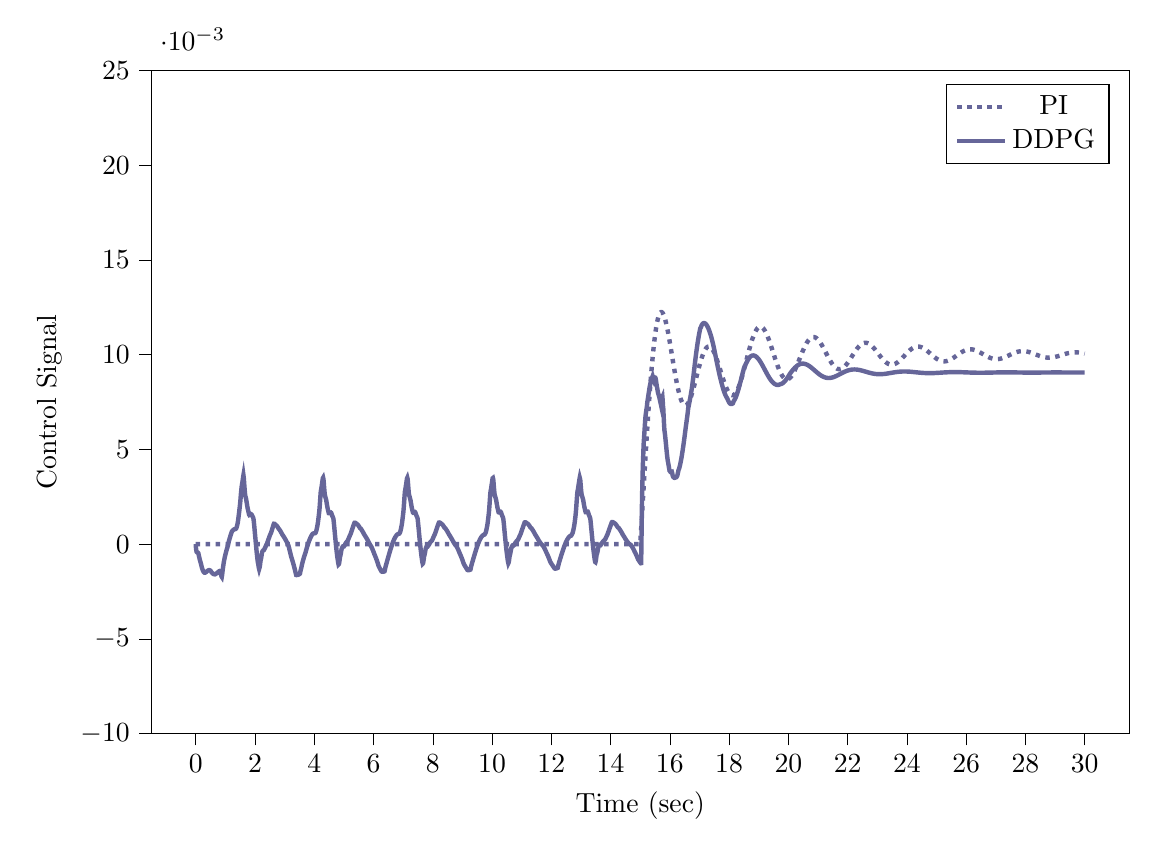
\begin{tikzpicture}

\definecolor{color0}{rgb}{0.12156862745098,0.466666666666667,0.705882352941177}
\definecolor{color1}{rgb}{1,0.498039215686275,0.0549019607843137}

\begin{axis}[
compat=newest,
tick align=outside,
tick pos=left,
x grid style={white!69.0196078431373!black},
xmin=-1.50000000000009, xmax=31.500000000002,
xtick style={color=black},
y grid style={white!69.0196078431373!black},
ymin=-0.01, ymax=0.025,
ytick style={color=black},
%yticklabel style={
%        /pgf/number format/.cd,
%        	fixed,
%        	fixed zerofill,
%         	precision=3,
%        /tikz/.cd
%},
scaled y ticks=true,
scaled y ticks=base 10:3,
width=14cm,
height=10cm,
xlabel=Time (sec),
ylabel=Control Signal
%y label style={at={(-0.2,0.5)}}
]

\addplot [ultra thick, blue!20!gray, dotted]
table {%
0 0
0.01 0
0.02 0
0.03 0
0.04 0
0.05 0
0.06 0
0.07 0
0.08 0
0.09 0
0.1 0
0.11 0
0.12 0
0.13 0
0.14 0
0.15 0
0.16 0
0.17 0
0.18 0
0.19 0
0.2 0
0.21 0
0.22 0
0.23 0
0.24 0
0.25 0
0.26 0
0.27 0
0.28 0
0.29 0
0.3 0
0.31 0
0.32 0
0.33 0
0.34 0
0.35 0
0.36 0
0.37 0
0.38 0
0.39 0
0.4 0
0.41 0
0.42 0
0.43 0
0.44 0
0.45 0
0.46 0
0.47 0
0.48 0
0.49 0
0.5 0
0.51 0
0.52 0
0.53 0
0.54 0
0.55 0
0.56 0
0.57 0
0.58 0
0.59 0
0.6 0
0.61 0
0.62 0
0.63 0
0.64 0
0.65 0
0.66 0
0.67 0
0.68 0
0.69 0
0.7 0
0.71 0
0.72 0
0.73 0
0.74 0
0.75 0
0.76 0
0.77 0
0.78 0
0.79 0
0.8 0
0.81 0
0.820000000000001 0
0.830000000000001 0
0.840000000000001 0
0.850000000000001 0
0.860000000000001 0
0.870000000000001 0
0.880000000000001 0
0.890000000000001 0
0.900000000000001 0
0.910000000000001 0
0.920000000000001 0
0.930000000000001 0
0.940000000000001 0
0.950000000000001 0
0.960000000000001 0
0.970000000000001 0
0.980000000000001 0
0.990000000000001 0
1 0
1.01 0
1.02 0
1.03 0
1.04 0
1.05 0
1.06 0
1.07 0
1.08 0
1.09 0
1.1 0
1.11 0
1.12 0
1.13 0
1.14 0
1.15 0
1.16 0
1.17 0
1.18 0
1.19 0
1.2 0
1.21 0
1.22 0
1.23 0
1.24 0
1.25 0
1.26 0
1.27 0
1.28 0
1.29 0
1.3 0
1.31 0
1.32 0
1.33 0
1.34 0
1.35 0
1.36 0
1.37 0
1.38 0
1.39 0
1.4 0
1.41 0
1.42 0
1.43 0
1.44 0
1.45 0
1.46 0
1.47 0
1.48 0
1.49 0
1.5 0
1.51 0
1.52 0
1.53 0
1.54 0
1.55 0
1.56 0
1.57 0
1.58 0
1.59 0
1.6 0
1.61 0
1.62 0
1.63 0
1.64 0
1.65 0
1.66 0
1.67 0
1.68 0
1.69 0
1.7 0
1.71 0
1.72 0
1.73 0
1.74 0
1.75 0
1.76 0
1.77 0
1.78 0
1.79 0
1.8 0
1.81 0
1.82 0
1.83 0
1.84 0
1.85 0
1.86 0
1.87 0
1.88 0
1.89 0
1.9 0
1.91 0
1.92 0
1.93 0
1.94 0
1.95 0
1.96 0
1.97 0
1.98 0
1.99 0
2 0
2.01 0
2.02 0
2.03 0
2.04 0
2.05 0
2.06 0
2.07 0
2.08 0
2.09 0
2.1 0
2.11 0
2.12 0
2.13 0
2.14 0
2.15 0
2.16 0
2.17 0
2.18 0
2.19 0
2.2 0
2.21 0
2.22 0
2.23 0
2.24 0
2.25 0
2.26 0
2.27 0
2.28 0
2.29 0
2.29999999999999 0
2.30999999999999 0
2.31999999999999 0
2.32999999999999 0
2.33999999999999 0
2.34999999999999 0
2.35999999999999 0
2.36999999999999 0
2.37999999999999 0
2.38999999999999 0
2.39999999999999 0
2.40999999999999 0
2.41999999999999 0
2.42999999999999 0
2.43999999999999 0
2.44999999999999 0
2.45999999999999 0
2.46999999999999 0
2.47999999999999 0
2.48999999999999 0
2.49999999999999 0
2.50999999999999 0
2.51999999999999 0
2.52999999999999 0
2.53999999999999 0
2.54999999999999 0
2.55999999999999 0
2.56999999999999 0
2.57999999999999 0
2.58999999999999 0
2.59999999999999 0
2.60999999999999 0
2.61999999999999 0
2.62999999999999 0
2.63999999999999 0
2.64999999999999 0
2.65999999999999 0
2.66999999999999 0
2.67999999999999 0
2.68999999999999 0
2.69999999999999 0
2.70999999999999 0
2.71999999999999 0
2.72999999999999 0
2.73999999999999 0
2.74999999999999 0
2.75999999999999 0
2.76999999999998 0
2.77999999999998 0
2.78999999999998 0
2.79999999999998 0
2.80999999999998 0
2.81999999999998 0
2.82999999999998 0
2.83999999999998 0
2.84999999999998 0
2.85999999999998 0
2.86999999999998 0
2.87999999999998 0
2.88999999999998 0
2.89999999999998 0
2.90999999999998 0
2.91999999999998 0
2.92999999999998 0
2.93999999999998 0
2.94999999999998 0
2.95999999999998 0
2.96999999999998 0
2.97999999999998 0
2.98999999999998 0
2.99999999999998 0
3.00999999999998 0
3.01999999999998 0
3.02999999999998 0
3.03999999999998 0
3.04999999999998 0
3.05999999999998 0
3.06999999999998 0
3.07999999999998 0
3.08999999999998 0
3.09999999999998 0
3.10999999999998 0
3.11999999999998 0
3.12999999999998 0
3.13999999999998 0
3.14999999999998 0
3.15999999999998 0
3.16999999999998 0
3.17999999999998 0
3.18999999999998 0
3.19999999999998 0
3.20999999999998 0
3.21999999999998 0
3.22999999999998 0
3.23999999999997 0
3.24999999999997 0
3.25999999999997 0
3.26999999999997 0
3.27999999999997 0
3.28999999999997 0
3.29999999999997 0
3.30999999999997 0
3.31999999999997 0
3.32999999999997 0
3.33999999999997 0
3.34999999999997 0
3.35999999999997 0
3.36999999999997 0
3.37999999999997 0
3.38999999999997 0
3.39999999999997 0
3.40999999999997 0
3.41999999999997 0
3.42999999999997 0
3.43999999999997 0
3.44999999999997 0
3.45999999999997 0
3.46999999999997 0
3.47999999999997 0
3.48999999999997 0
3.49999999999997 0
3.50999999999997 0
3.51999999999997 0
3.52999999999997 0
3.53999999999997 0
3.54999999999997 0
3.55999999999997 0
3.56999999999997 0
3.57999999999997 0
3.58999999999997 0
3.59999999999997 0
3.60999999999997 0
3.61999999999997 0
3.62999999999997 0
3.63999999999997 0
3.64999999999997 0
3.65999999999997 0
3.66999999999997 0
3.67999999999997 0
3.68999999999997 0
3.69999999999997 0
3.70999999999996 0
3.71999999999996 0
3.72999999999996 0
3.73999999999996 0
3.74999999999996 0
3.75999999999996 0
3.76999999999996 0
3.77999999999996 0
3.78999999999996 0
3.79999999999996 0
3.80999999999996 0
3.81999999999996 0
3.82999999999996 0
3.83999999999996 0
3.84999999999996 0
3.85999999999996 0
3.86999999999996 0
3.87999999999996 0
3.88999999999996 0
3.89999999999996 0
3.90999999999996 0
3.91999999999996 0
3.92999999999996 0
3.93999999999996 0
3.94999999999996 0
3.95999999999996 0
3.96999999999996 0
3.97999999999996 0
3.98999999999996 0
3.99999999999996 0
4.00999999999996 0
4.01999999999996 0
4.02999999999996 0
4.03999999999996 0
4.04999999999996 0
4.05999999999996 0
4.06999999999996 0
4.07999999999996 0
4.08999999999996 0
4.09999999999996 0
4.10999999999996 0
4.11999999999996 0
4.12999999999996 0
4.13999999999996 0
4.14999999999996 0
4.15999999999996 0
4.16999999999996 0
4.17999999999996 0
4.18999999999996 0
4.19999999999995 0
4.20999999999995 0
4.21999999999995 0
4.22999999999995 0
4.23999999999995 0
4.24999999999995 0
4.25999999999995 0
4.26999999999995 0
4.27999999999995 0
4.28999999999995 0
4.29999999999995 0
4.30999999999995 0
4.31999999999995 0
4.32999999999995 0
4.33999999999995 0
4.34999999999995 0
4.35999999999995 0
4.36999999999995 0
4.37999999999995 0
4.38999999999995 0
4.39999999999995 0
4.40999999999995 0
4.41999999999995 0
4.42999999999995 0
4.43999999999995 0
4.44999999999995 0
4.45999999999995 0
4.46999999999995 0
4.47999999999995 0
4.48999999999995 0
4.49999999999995 0
4.50999999999995 0
4.51999999999995 0
4.52999999999995 0
4.53999999999995 0
4.54999999999995 0
4.55999999999995 0
4.56999999999995 0
4.57999999999995 0
4.58999999999995 0
4.59999999999995 0
4.60999999999995 0
4.61999999999995 0
4.62999999999995 0
4.63999999999995 0
4.64999999999995 0
4.65999999999995 0
4.66999999999994 0
4.67999999999994 0
4.68999999999994 0
4.69999999999994 0
4.70999999999994 0
4.71999999999994 0
4.72999999999994 0
4.73999999999994 0
4.74999999999994 0
4.75999999999994 0
4.76999999999994 0
4.77999999999994 0
4.78999999999994 0
4.79999999999994 0
4.80999999999994 0
4.81999999999994 0
4.82999999999994 0
4.83999999999994 0
4.84999999999994 0
4.85999999999994 0
4.86999999999994 0
4.87999999999994 0
4.88999999999994 0
4.89999999999994 0
4.90999999999994 0
4.91999999999994 0
4.92999999999994 0
4.93999999999994 0
4.94999999999994 0
4.95999999999994 0
4.96999999999994 0
4.97999999999994 0
4.98999999999994 0
4.99999999999994 0
5.00999999999994 0
5.01999999999994 0
5.02999999999994 0
5.03999999999994 0
5.04999999999994 0
5.05999999999994 0
5.06999999999994 0
5.07999999999994 0
5.08999999999994 0
5.09999999999994 0
5.10999999999994 0
5.11999999999994 0
5.12999999999994 0
5.13999999999993 0
5.14999999999993 0
5.15999999999993 0
5.16999999999993 0
5.17999999999993 0
5.18999999999993 0
5.19999999999993 0
5.20999999999993 0
5.21999999999993 0
5.22999999999993 0
5.23999999999993 0
5.24999999999993 0
5.25999999999993 0
5.26999999999993 0
5.27999999999993 0
5.28999999999993 0
5.29999999999993 0
5.30999999999993 0
5.31999999999993 0
5.32999999999993 0
5.33999999999993 0
5.34999999999993 0
5.35999999999993 0
5.36999999999993 0
5.37999999999993 0
5.38999999999993 0
5.39999999999993 0
5.40999999999993 0
5.41999999999993 0
5.42999999999993 0
5.43999999999993 0
5.44999999999993 0
5.45999999999993 0
5.46999999999993 0
5.47999999999993 0
5.48999999999993 0
5.49999999999993 0
5.50999999999993 0
5.51999999999993 0
5.52999999999993 0
5.53999999999993 0
5.54999999999993 0
5.55999999999993 0
5.56999999999993 0
5.57999999999993 0
5.58999999999993 0
5.59999999999993 0
5.60999999999992 0
5.61999999999992 0
5.62999999999992 0
5.63999999999992 0
5.64999999999992 0
5.65999999999992 0
5.66999999999992 0
5.67999999999992 0
5.68999999999992 0
5.69999999999992 0
5.70999999999992 0
5.71999999999992 0
5.72999999999992 0
5.73999999999992 0
5.74999999999992 0
5.75999999999992 0
5.76999999999992 0
5.77999999999992 0
5.78999999999992 0
5.79999999999992 0
5.80999999999992 0
5.81999999999992 0
5.82999999999992 0
5.83999999999992 0
5.84999999999992 0
5.85999999999992 0
5.86999999999992 0
5.87999999999992 0
5.88999999999992 0
5.89999999999992 0
5.90999999999992 0
5.91999999999992 0
5.92999999999992 0
5.93999999999992 0
5.94999999999992 0
5.95999999999992 0
5.96999999999992 0
5.97999999999992 0
5.98999999999992 0
5.99999999999992 0
6.00999999999992 0
6.01999999999992 0
6.02999999999992 0
6.03999999999992 0
6.04999999999992 0
6.05999999999992 0
6.06999999999992 0
6.07999999999991 0
6.08999999999991 0
6.09999999999991 0
6.10999999999991 0
6.11999999999991 0
6.12999999999991 0
6.13999999999991 0
6.14999999999991 0
6.15999999999991 0
6.16999999999991 0
6.17999999999991 0
6.18999999999991 0
6.19999999999991 0
6.20999999999991 0
6.21999999999991 0
6.22999999999991 0
6.23999999999991 0
6.24999999999991 0
6.25999999999991 0
6.26999999999991 0
6.27999999999991 0
6.28999999999991 0
6.29999999999991 0
6.30999999999991 0
6.31999999999991 0
6.32999999999991 0
6.33999999999991 0
6.34999999999991 0
6.35999999999991 0
6.36999999999991 0
6.37999999999991 0
6.38999999999991 0
6.39999999999991 0
6.40999999999991 0
6.41999999999991 0
6.42999999999991 0
6.43999999999991 0
6.44999999999991 0
6.45999999999991 0
6.46999999999991 0
6.47999999999991 0
6.48999999999991 0
6.49999999999991 0
6.50999999999991 0
6.51999999999991 0
6.52999999999991 0
6.53999999999991 0
6.5499999999999 0
6.5599999999999 0
6.5699999999999 0
6.5799999999999 0
6.5899999999999 0
6.5999999999999 0
6.6099999999999 0
6.6199999999999 0
6.6299999999999 0
6.6399999999999 0
6.6499999999999 0
6.6599999999999 0
6.6699999999999 0
6.6799999999999 0
6.6899999999999 0
6.6999999999999 0
6.7099999999999 0
6.7199999999999 0
6.7299999999999 0
6.7399999999999 0
6.7499999999999 0
6.7599999999999 0
6.7699999999999 0
6.7799999999999 0
6.7899999999999 0
6.7999999999999 0
6.8099999999999 0
6.8199999999999 0
6.8299999999999 0
6.8399999999999 0
6.8499999999999 0
6.8599999999999 0
6.8699999999999 0
6.8799999999999 0
6.8899999999999 0
6.8999999999999 0
6.9099999999999 0
6.9199999999999 0
6.9299999999999 0
6.9399999999999 0
6.9499999999999 0
6.9599999999999 0
6.9699999999999 0
6.9799999999999 0
6.9899999999999 0
6.9999999999999 0
7.00999999999989 0
7.01999999999989 0
7.02999999999989 0
7.03999999999989 0
7.04999999999989 0
7.05999999999989 0
7.06999999999989 0
7.07999999999989 0
7.08999999999989 0
7.09999999999989 0
7.10999999999989 0
7.11999999999989 0
7.12999999999989 0
7.13999999999989 0
7.14999999999989 0
7.15999999999989 0
7.16999999999989 0
7.17999999999989 0
7.18999999999989 0
7.19999999999989 0
7.20999999999989 0
7.21999999999989 0
7.22999999999989 0
7.23999999999989 0
7.24999999999989 0
7.25999999999989 0
7.26999999999989 0
7.27999999999989 0
7.28999999999989 0
7.29999999999989 0
7.30999999999989 0
7.31999999999989 0
7.32999999999989 0
7.33999999999989 0
7.34999999999989 0
7.35999999999989 0
7.36999999999989 0
7.37999999999989 0
7.38999999999989 0
7.39999999999989 0
7.40999999999989 0
7.41999999999989 0
7.42999999999989 0
7.43999999999989 0
7.44999999999989 0
7.45999999999989 0
7.46999999999989 0
7.47999999999988 0
7.48999999999988 0
7.49999999999988 0
7.50999999999988 0
7.51999999999988 0
7.52999999999988 0
7.53999999999988 0
7.54999999999988 0
7.55999999999988 0
7.56999999999988 0
7.57999999999988 0
7.58999999999988 0
7.59999999999988 0
7.60999999999988 0
7.61999999999988 0
7.62999999999988 0
7.63999999999988 0
7.64999999999988 0
7.65999999999988 0
7.66999999999988 0
7.67999999999988 0
7.68999999999988 0
7.69999999999988 0
7.70999999999988 0
7.71999999999988 0
7.72999999999988 0
7.73999999999988 0
7.74999999999988 0
7.75999999999988 0
7.76999999999988 0
7.77999999999988 0
7.78999999999988 0
7.79999999999988 0
7.80999999999988 0
7.81999999999988 0
7.82999999999988 0
7.83999999999988 0
7.84999999999988 0
7.85999999999988 0
7.86999999999988 0
7.87999999999988 0
7.88999999999988 0
7.89999999999988 0
7.90999999999988 0
7.91999999999988 0
7.92999999999988 0
7.93999999999988 0
7.94999999999987 0
7.95999999999987 0
7.96999999999987 0
7.97999999999987 0
7.98999999999987 0
7.99999999999987 0
8.00999999999987 0
8.01999999999987 0
8.02999999999987 0
8.03999999999987 0
8.04999999999987 0
8.05999999999987 0
8.06999999999987 0
8.07999999999987 0
8.08999999999987 0
8.09999999999987 0
8.10999999999987 0
8.11999999999987 0
8.12999999999987 0
8.13999999999987 0
8.14999999999987 0
8.15999999999987 0
8.16999999999987 0
8.17999999999987 0
8.18999999999987 0
8.19999999999987 0
8.20999999999987 0
8.21999999999987 0
8.22999999999987 0
8.23999999999987 0
8.24999999999987 0
8.25999999999987 0
8.26999999999987 0
8.27999999999987 0
8.28999999999987 0
8.29999999999987 0
8.30999999999987 0
8.31999999999987 0
8.32999999999987 0
8.33999999999987 0
8.34999999999987 0
8.35999999999987 0
8.36999999999987 0
8.37999999999987 0
8.38999999999987 0
8.39999999999987 0
8.40999999999987 0
8.41999999999986 0
8.42999999999986 0
8.43999999999986 0
8.44999999999986 0
8.45999999999986 0
8.46999999999986 0
8.47999999999986 0
8.48999999999986 0
8.49999999999986 0
8.50999999999986 0
8.51999999999986 0
8.52999999999986 0
8.53999999999986 0
8.54999999999986 0
8.55999999999986 0
8.56999999999986 0
8.57999999999986 0
8.58999999999986 0
8.59999999999986 0
8.60999999999986 0
8.61999999999986 0
8.62999999999986 0
8.63999999999986 0
8.64999999999986 0
8.65999999999986 0
8.66999999999986 0
8.67999999999986 0
8.68999999999986 0
8.69999999999986 0
8.70999999999986 0
8.71999999999986 0
8.72999999999986 0
8.73999999999986 0
8.74999999999986 0
8.75999999999986 0
8.76999999999986 0
8.77999999999986 0
8.78999999999986 0
8.79999999999986 0
8.80999999999986 0
8.81999999999986 0
8.82999999999986 0
8.83999999999986 0
8.84999999999986 0
8.85999999999986 0
8.86999999999986 0
8.87999999999986 0
8.88999999999985 0
8.89999999999985 0
8.90999999999985 0
8.91999999999985 0
8.92999999999985 0
8.93999999999985 0
8.94999999999985 0
8.95999999999985 0
8.96999999999985 0
8.97999999999985 0
8.98999999999985 0
8.99999999999985 0
9.00999999999985 0
9.01999999999985 0
9.02999999999985 0
9.03999999999985 0
9.04999999999985 0
9.05999999999985 0
9.06999999999985 0
9.07999999999985 0
9.08999999999985 0
9.09999999999985 0
9.10999999999985 0
9.11999999999985 0
9.12999999999985 0
9.13999999999985 0
9.14999999999985 0
9.15999999999985 0
9.16999999999985 0
9.17999999999985 0
9.18999999999985 0
9.19999999999985 0
9.20999999999985 0
9.21999999999985 0
9.22999999999985 0
9.23999999999985 0
9.24999999999985 0
9.25999999999985 0
9.26999999999985 0
9.27999999999985 0
9.28999999999985 0
9.29999999999985 0
9.30999999999985 0
9.31999999999985 0
9.32999999999985 0
9.33999999999985 0
9.34999999999985 0
9.35999999999984 0
9.36999999999984 0
9.37999999999984 0
9.38999999999984 0
9.39999999999984 0
9.40999999999984 0
9.41999999999984 0
9.42999999999984 0
9.43999999999984 0
9.44999999999984 0
9.45999999999984 0
9.46999999999984 0
9.47999999999984 0
9.48999999999984 0
9.49999999999984 0
9.50999999999984 0
9.51999999999984 0
9.52999999999984 0
9.53999999999984 0
9.54999999999984 0
9.55999999999984 0
9.56999999999984 0
9.57999999999984 0
9.58999999999984 0
9.59999999999984 0
9.60999999999984 0
9.61999999999984 0
9.62999999999984 0
9.63999999999984 0
9.64999999999984 0
9.65999999999984 0
9.66999999999984 0
9.67999999999984 0
9.68999999999984 0
9.69999999999984 0
9.70999999999984 0
9.71999999999984 0
9.72999999999984 0
9.73999999999984 0
9.74999999999984 0
9.75999999999984 0
9.76999999999984 0
9.77999999999984 0
9.78999999999984 0
9.79999999999984 0
9.80999999999984 0
9.81999999999984 0
9.82999999999983 0
9.83999999999983 0
9.84999999999983 0
9.85999999999983 0
9.86999999999983 0
9.87999999999983 0
9.88999999999983 0
9.89999999999983 0
9.90999999999983 0
9.91999999999983 0
9.92999999999983 0
9.93999999999983 0
9.94999999999983 0
9.95999999999983 0
9.96999999999983 0
9.97999999999983 0
9.98999999999983 0
9.99999999999983 0
10.0099999999998 0
10.0199999999998 0
10.0299999999998 0
10.0399999999998 0
10.0499999999998 0
10.0599999999998 0
10.0699999999998 0
10.0799999999998 0
10.0899999999998 0
10.0999999999998 0
10.1099999999998 0
10.1199999999998 0
10.1299999999998 0
10.1399999999998 0
10.1499999999998 0
10.1599999999998 0
10.1699999999998 0
10.1799999999998 0
10.1899999999998 0
10.1999999999998 0
10.2099999999998 0
10.2199999999998 0
10.2299999999998 0
10.2399999999998 0
10.2499999999998 0
10.2599999999998 0
10.2699999999998 0
10.2799999999998 0
10.2899999999998 0
10.2999999999998 0
10.3099999999998 0
10.3199999999998 0
10.3299999999998 0
10.3399999999998 0
10.3499999999998 0
10.3599999999998 0
10.3699999999998 0
10.3799999999998 0
10.3899999999998 0
10.3999999999998 0
10.4099999999998 0
10.4199999999998 0
10.4299999999998 0
10.4399999999998 0
10.4499999999998 0
10.4599999999998 0
10.4699999999998 0
10.4799999999998 0
10.4899999999998 0
10.4999999999998 0
10.5099999999998 0
10.5199999999998 0
10.5299999999998 0
10.5399999999998 0
10.5499999999998 0
10.5599999999998 0
10.5699999999998 0
10.5799999999998 0
10.5899999999998 0
10.5999999999998 0
10.6099999999998 0
10.6199999999998 0
10.6299999999998 0
10.6399999999998 0
10.6499999999998 0
10.6599999999998 0
10.6699999999998 0
10.6799999999998 0
10.6899999999998 0
10.6999999999998 0
10.7099999999998 0
10.7199999999998 0
10.7299999999998 0
10.7399999999998 0
10.7499999999998 0
10.7599999999998 0
10.7699999999998 0
10.7799999999998 0
10.7899999999998 0
10.7999999999998 0
10.8099999999998 0
10.8199999999998 0
10.8299999999998 0
10.8399999999998 0
10.8499999999998 0
10.8599999999998 0
10.8699999999998 0
10.8799999999998 0
10.8899999999998 0
10.8999999999998 0
10.9099999999998 0
10.9199999999998 0
10.9299999999998 0
10.9399999999998 0
10.9499999999998 0
10.9599999999998 0
10.9699999999998 0
10.9799999999998 0
10.9899999999998 0
10.9999999999998 0
11.0099999999998 0
11.0199999999998 0
11.0299999999998 0
11.0399999999998 0
11.0499999999998 0
11.0599999999998 0
11.0699999999998 0
11.0799999999998 0
11.0899999999998 0
11.0999999999998 0
11.1099999999998 0
11.1199999999998 0
11.1299999999998 0
11.1399999999998 0
11.1499999999998 0
11.1599999999998 0
11.1699999999998 0
11.1799999999998 0
11.1899999999998 0
11.1999999999998 0
11.2099999999998 0
11.2199999999998 0
11.2299999999998 0
11.2399999999998 0
11.2499999999998 0
11.2599999999998 0
11.2699999999998 0
11.2799999999998 0
11.2899999999998 0
11.2999999999998 0
11.3099999999998 0
11.3199999999998 0
11.3299999999998 0
11.3399999999998 0
11.3499999999998 0
11.3599999999998 0
11.3699999999998 0
11.3799999999998 0
11.3899999999998 0
11.3999999999998 0
11.4099999999998 0
11.4199999999998 0
11.4299999999998 0
11.4399999999998 0
11.4499999999998 0
11.4599999999998 0
11.4699999999998 0
11.4799999999998 0
11.4899999999998 0
11.4999999999998 0
11.5099999999998 0
11.5199999999998 0
11.5299999999998 0
11.5399999999998 0
11.5499999999998 0
11.5599999999998 0
11.5699999999998 0
11.5799999999998 0
11.5899999999998 0
11.5999999999998 0
11.6099999999998 0
11.6199999999998 0
11.6299999999998 0
11.6399999999998 0
11.6499999999998 0
11.6599999999998 0
11.6699999999998 0
11.6799999999998 0
11.6899999999998 0
11.6999999999998 0
11.7099999999998 0
11.7199999999998 0
11.7299999999998 0
11.7399999999998 0
11.7499999999998 0
11.7599999999998 0
11.7699999999998 0
11.7799999999998 0
11.7899999999998 0
11.7999999999998 0
11.8099999999998 0
11.8199999999998 0
11.8299999999998 0
11.8399999999998 0
11.8499999999998 0
11.8599999999998 0
11.8699999999998 0
11.8799999999998 0
11.8899999999998 0
11.8999999999998 0
11.9099999999998 0
11.9199999999998 0
11.9299999999998 0
11.9399999999998 0
11.9499999999998 0
11.9599999999998 0
11.9699999999998 0
11.9799999999998 0
11.9899999999998 0
11.9999999999998 0
12.0099999999998 0
12.0199999999998 0
12.0299999999998 0
12.0399999999998 0
12.0499999999998 0
12.0599999999998 0
12.0699999999998 0
12.0799999999998 0
12.0899999999998 0
12.0999999999998 0
12.1099999999998 0
12.1199999999998 0
12.1299999999998 0
12.1399999999998 0
12.1499999999998 0
12.1599999999998 0
12.1699999999998 0
12.1799999999998 0
12.1899999999998 0
12.1999999999998 0
12.2099999999998 0
12.2199999999998 0
12.2299999999998 0
12.2399999999998 0
12.2499999999998 0
12.2599999999998 0
12.2699999999998 0
12.2799999999998 0
12.2899999999998 0
12.2999999999998 0
12.3099999999998 0
12.3199999999998 0
12.3299999999998 0
12.3399999999998 0
12.3499999999998 0
12.3599999999998 0
12.3699999999998 0
12.3799999999998 0
12.3899999999998 0
12.3999999999998 0
12.4099999999998 0
12.4199999999998 0
12.4299999999998 0
12.4399999999998 0
12.4499999999998 0
12.4599999999998 0
12.4699999999998 0
12.4799999999998 0
12.4899999999998 0
12.4999999999998 0
12.5099999999998 0
12.5199999999998 0
12.5299999999998 0
12.5399999999998 0
12.5499999999998 0
12.5599999999998 0
12.5699999999998 0
12.5799999999998 0
12.5899999999998 0
12.5999999999998 0
12.6099999999998 0
12.6199999999998 0
12.6299999999998 0
12.6399999999998 0
12.6499999999998 0
12.6599999999998 0
12.6699999999998 0
12.6799999999998 0
12.6899999999998 0
12.6999999999998 0
12.7099999999998 0
12.7199999999998 0
12.7299999999998 0
12.7399999999998 0
12.7499999999998 0
12.7599999999998 0
12.7699999999998 0
12.7799999999998 0
12.7899999999998 0
12.7999999999998 0
12.8099999999998 0
12.8199999999998 0
12.8299999999998 0
12.8399999999998 0
12.8499999999998 0
12.8599999999998 0
12.8699999999998 0
12.8799999999998 0
12.8899999999998 0
12.8999999999998 0
12.9099999999998 0
12.9199999999998 0
12.9299999999998 0
12.9399999999998 0
12.9499999999998 0
12.9599999999998 0
12.9699999999998 0
12.9799999999998 0
12.9899999999998 0
12.9999999999998 0
13.0099999999998 0
13.0199999999998 0
13.0299999999998 0
13.0399999999998 0
13.0499999999998 0
13.0599999999998 0
13.0699999999998 0
13.0799999999998 0
13.0899999999998 0
13.0999999999998 0
13.1099999999998 0
13.1199999999998 0
13.1299999999998 0
13.1399999999998 0
13.1499999999998 0
13.1599999999998 0
13.1699999999998 0
13.1799999999998 0
13.1899999999998 0
13.1999999999998 0
13.2099999999998 0
13.2199999999998 0
13.2299999999998 0
13.2399999999998 0
13.2499999999998 0
13.2599999999998 0
13.2699999999998 0
13.2799999999998 0
13.2899999999998 0
13.2999999999998 0
13.3099999999998 0
13.3199999999998 0
13.3299999999998 0
13.3399999999998 0
13.3499999999998 0
13.3599999999998 0
13.3699999999998 0
13.3799999999998 0
13.3899999999998 0
13.3999999999998 0
13.4099999999998 0
13.4199999999998 0
13.4299999999998 0
13.4399999999998 0
13.4499999999998 0
13.4599999999998 0
13.4699999999998 0
13.4799999999998 0
13.4899999999998 0
13.4999999999998 0
13.5099999999998 0
13.5199999999998 0
13.5299999999998 0
13.5399999999998 0
13.5499999999998 0
13.5599999999998 0
13.5699999999998 0
13.5799999999998 0
13.5899999999998 0
13.5999999999998 0
13.6099999999998 0
13.6199999999998 0
13.6299999999998 0
13.6399999999998 0
13.6499999999998 0
13.6599999999998 0
13.6699999999998 0
13.6799999999998 0
13.6899999999998 0
13.6999999999998 0
13.7099999999998 0
13.7199999999998 0
13.7299999999998 0
13.7399999999998 0
13.7499999999998 0
13.7599999999998 0
13.7699999999998 0
13.7799999999998 0
13.7899999999998 0
13.7999999999998 0
13.8099999999998 0
13.8199999999997 0
13.8299999999997 0
13.8399999999997 0
13.8499999999997 0
13.8599999999997 0
13.8699999999997 0
13.8799999999997 0
13.8899999999997 0
13.8999999999997 0
13.9099999999997 0
13.9199999999997 0
13.9299999999997 0
13.9399999999997 0
13.9499999999997 0
13.9599999999997 0
13.9699999999997 0
13.9799999999997 0
13.9899999999997 0
13.9999999999997 0
14.0099999999997 0
14.0199999999997 0
14.0299999999997 0
14.0399999999997 0
14.0499999999997 0
14.0599999999997 0
14.0699999999997 0
14.0799999999997 0
14.0899999999997 0
14.0999999999997 0
14.1099999999997 0
14.1199999999997 0
14.1299999999997 0
14.1399999999997 0
14.1499999999997 0
14.1599999999997 0
14.1699999999997 0
14.1799999999997 0
14.1899999999997 0
14.1999999999997 0
14.2099999999997 0
14.2199999999997 0
14.2299999999997 0
14.2399999999997 0
14.2499999999997 0
14.2599999999997 0
14.2699999999997 0
14.2799999999997 0
14.2899999999997 0
14.2999999999997 0
14.3099999999997 0
14.3199999999997 0
14.3299999999997 0
14.3399999999997 0
14.3499999999997 0
14.3599999999997 0
14.3699999999997 0
14.3799999999997 0
14.3899999999997 0
14.3999999999997 0
14.4099999999997 0
14.4199999999997 0
14.4299999999997 0
14.4399999999997 0
14.4499999999997 0
14.4599999999997 0
14.4699999999997 0
14.4799999999997 0
14.4899999999997 0
14.4999999999997 0
14.5099999999997 0
14.5199999999997 0
14.5299999999997 0
14.5399999999997 0
14.5499999999997 0
14.5599999999997 0
14.5699999999997 0
14.5799999999997 0
14.5899999999997 0
14.5999999999997 0
14.6099999999997 0
14.6199999999997 0
14.6299999999997 0
14.6399999999997 0
14.6499999999997 0
14.6599999999997 0
14.6699999999997 0
14.6799999999997 0
14.6899999999997 0
14.6999999999997 0
14.7099999999997 0
14.7199999999997 0
14.7299999999997 0
14.7399999999997 0
14.7499999999997 0
14.7599999999997 0
14.7699999999997 0
14.7799999999997 0
14.7899999999997 0
14.7999999999997 0
14.8099999999997 0
14.8199999999997 0
14.8299999999997 0
14.8399999999997 0
14.8499999999997 0
14.8599999999997 0
14.8699999999997 0
14.8799999999997 0
14.8899999999997 0
14.8999999999997 0
14.9099999999997 0
14.9199999999997 0
14.9299999999997 0
14.9399999999997 0
14.9499999999997 0
14.9599999999997 0
14.9699999999997 0
14.9799999999997 0
14.9899999999997 0
14.9999999999997 1.65143933586237e-09
15.0099999999997 0.000251646628705991
15.0199999999997 0.000504813715529082
15.0299999999997 0.000759409495223724
15.0399999999997 0.0010153171453592
15.0499999999997 0.00127240160730084
15.0599999999997 0.00153051202950275
15.0699999999997 0.0017894842012412
15.0799999999997 0.00204914261052369
15.0899999999997 0.00230930228873294
15.0999999999997 0.00256977047864943
15.1099999999997 0.00283034812071255
15.1199999999997 0.00309083117851801
15.1299999999997 0.00335101182327691
15.1399999999997 0.00361067949426346
15.1499999999997 0.00386962185004272
15.1599999999997 0.00412762562336092
15.1699999999997 0.00438447739093926
15.1799999999997 0.00463996426797917
15.1899999999997 0.0048938745359416
15.1999999999997 0.00514599821107789
15.2099999999997 0.00539612756023699
15.2199999999997 0.00564405756964693
15.2299999999997 0.0058895863716423
15.2399999999997 0.00613251563367615
15.2499999999997 0.00637265091340354
15.2599999999997 0.0066098019831371
15.2699999999997 0.00684378312655668
15.2799999999997 0.00707441341018548
15.2899999999997 0.00730151693182289
15.2999999999997 0.00752492304784595
15.3099999999997 0.0077444665810465
15.3199999999997 0.00795998801045696
15.3299999999997 0.00817133364443574
15.3399999999997 0.0083783557781198
15.3499999999997 0.0085809128362127
15.3599999999997 0.00877886950195709
15.3699999999997 0.00897209683303236
15.3799999999997 0.00916047236503106
15.3899999999997 0.00934388020308567
15.3999999999997 0.0095222111021532
15.4099999999997 0.00969536253640429
15.4199999999997 0.00986323875811496
15.4299999999997 0.0100257508464171
15.4399999999997 0.010182816746761
15.4499999999997 0.0103343612993197
15.4599999999997 0.0104803162594725
15.4699999999997 0.0106206203089849
15.4799999999997 0.0107552190583435
15.4899999999997 0.0108840650409438
15.4999999999997 0.0110071176972975
15.5099999999997 0.011124343352648
15.5199999999997 0.0112357151860114
15.5299999999997 0.0113412131913552
15.5399999999997 0.0114408241310805
15.5499999999997 0.0115345414819743
15.5599999999997 0.0116223653737919
15.5699999999997 0.0117043025206279
15.5799999999997 0.0117803661451226
15.5899999999997 0.0118505758952864
15.5999999999997 0.0119149579143133
15.6099999999997 0.0119735446087437
15.6199999999997 0.0120263743730305
15.6299999999997 0.0120734916350397
15.6399999999997 0.0121149467423113
15.6499999999997 0.0121507958425362
15.6599999999997 0.0121811007584378
15.6699999999997 0.0122059288572524
15.6799999999997 0.0122253529150019
15.6899999999997 0.0122394509757588
15.6999999999997 0.0122483062073349
15.7099999999997 0.0122520067746912
15.7199999999997 0.0122506459870169
15.7299999999997 0.0122443214434493
15.7399999999997 0.0122331352385886
15.7499999999997 0.0122171937960714
15.7599999999997 0.0121966076985984
15.7699999999997 0.0121714915146394
15.7799999999997 0.0121419636227105
15.7899999999997 0.0121081460308243
15.7999999999997 0.0120701641950366
15.8099999999997 0.0120281468355185
15.8199999999997 0.0119822257500982
15.8299999999997 0.0119325356249662
15.8399999999997 0.0118792138450612
15.8499999999997 0.0118224003024289
15.8599999999997 0.0117622372033321
15.8699999999997 0.0116988688743441
15.8799999999997 0.0116324415676611
15.8899999999997 0.0115631032658651
15.8999999999997 0.0114910034863693
15.9099999999997 0.0114162930857789
15.9199999999997 0.0113391240643967
15.9299999999997 0.0112596493713743
15.9399999999997 0.0111780227107287
15.9499999999997 0.0110943983459273
15.9599999999997 0.0110089309081382
15.9699999999997 0.0109217752048475
15.9799999999997 0.0108330860299626
15.9899999999997 0.010743017975616
15.9999999999997 0.0106517252458821
16.0099999999997 0.0105593614726147
16.0199999999997 0.010466079533611
16.0299999999997 0.0103720313733037
16.0399999999997 0.0102773678261791
16.0499999999997 0.0101822384431166
16.0599999999997 0.0100867913207596
16.0699999999997 0.00999117282763884
16.0799999999997 0.00989552761682951
16.0899999999997 0.00979999839634916
16.0999999999997 0.009704725772254
16.1099999999997 0.00960984809572078
16.1199999999997 0.00951550131426175
16.1299999999997 0.00942181882721364
16.1399999999997 0.00932893134564011
16.1499999999997 0.00923696675677972
16.1599999999997 0.00914604999316607
16.1699999999997 0.00905630290654273
16.1799999999997 0.00896784414668765
16.1899999999997 0.00888078904525547
16.1999999999997 0.00879524950474298
16.2099999999997 0.00871133389267151
16.2199999999997 0.00862914694107768
16.2299999999997 0.00854878965139488
16.2399999999997 0.00847035920480175
16.2499999999997 0.00839394887810764
16.2599999999997 0.00831964796523675
16.2699999999997 0.00824754170436735
16.2799999999997 0.008177711210774
16.2899999999997 0.00811023341541516
16.2999999999997 0.00804518100930091
16.3099999999998 0.00798262239366929
16.3199999999998 0.00792262159736296
16.3299999999998 0.00786523821083156
16.3399999999998 0.00781052751081816
16.3499999999998 0.0077585403426363
16.3599999999998 0.00770932304518571
16.3699999999998 0.00766291745392498
16.3799999999998 0.00761936101587842
16.3899999999998 0.0075786866982003
16.3999999999998 0.00754092299039499
16.4099999999998 0.00750609391217645
16.4199999999998 0.00747421902746872
16.4299999999998 0.00744531346441154
16.4399999999998 0.00741938793560937
16.4499999999998 0.00739644877097179
16.4599999999998 0.00737649795300926
16.4699999999998 0.007359533157394
16.4799999999998 0.00734554780005938
16.4899999999998 0.00733453108596858
16.4999999999998 0.00732646806304129
16.5099999999998 0.00732133968568659
16.5199999999998 0.00731912288018435
16.5299999999998 0.00731979021864938
16.5399999999998 0.00732331066143274
16.5499999999998 0.00732964953970922
16.5599999999998 0.00733876845866182
16.5699999999998 0.00735062538578098
16.5799999999998 0.00736517474296724
16.5899999999998 0.00738236750233981
16.5999999999998 0.00740215128563695
16.6099999999998 0.00742447046708126
16.6199999999998 0.00744926627957387
16.6299999999998 0.00747647692407254
16.6399999999998 0.00750603768200355
16.6499999999998 0.00753788102880218
16.6599999999998 0.00757193675519417
16.6699999999998 0.00760813208638035
16.6799999999998 0.0076463918048768
16.6899999999998 0.00768663837567033
16.6999999999998 0.00772879207341752
16.7099999999998 0.00777277111151301
16.7199999999998 0.00781849177285081
16.7299999999998 0.00786586854210142
16.7399999999998 0.00791481423932581
16.7499999999998 0.00796524015474771
16.7599999999998 0.00801705618450379
16.7699999999998 0.00807017096719201
16.7799999999998 0.00812449202103842
16.7899999999998 0.00817992588150534
16.7999999999998 0.00823637823918295
16.8099999999998 0.00829375407769597
16.8199999999998 0.00835195781154313
16.8299999999998 0.00841089342367419
16.8399999999998 0.00847046460261877
16.8499999999998 0.00853057487899296
16.8599999999998 0.00859112776121231
16.8699999999998 0.00865202687024156
16.8799999999998 0.00871317607321355
16.8899999999998 0.00877447961575266
16.8999999999998 0.00883584225283994
16.9099999999998 0.00889716937806082
16.9199999999998 0.00895836715107769
16.9299999999998 0.00901934262317827
16.9399999999998 0.00908000386074412
16.9499999999999 0.00914026006649596
16.9599999999999 0.00920002169835777
16.9699999999999 0.00925920058579342
16.9799999999999 0.00931771004357101
16.9899999999999 0.00937546498272624
16.9999999999999 0.00943238201862552
17.0099999999999 0.00948837957600957
17.0199999999999 0.00954337799089992
17.0299999999999 0.00959729960925543
17.0399999999999 0.00965006888227058
17.0499999999999 0.00970161245821259
17.0599999999999 0.00975185927069889
17.0699999999999 0.00980074062332166
17.0799999999999 0.00984819027053153
17.0899999999999 0.00989414449469739
17.0999999999999 0.00993854217900834
17.1099999999999 0.00998132487436766
17.1199999999999 0.0100224368699089
17.1299999999999 0.0100618252514182
17.1399999999999 0.0100994399579998
17.1499999999999 0.0101352338347464
17.1599999999999 0.010169162681151
17.1699999999999 0.010201185295265
17.1799999999999 0.0102312635136516
17.1899999999999 0.0102593622462963
17.1999999999999 0.0102854495078829
17.2099999999999 0.0103094966656106
17.2199999999999 0.0103314780482327
17.2299999999999 0.0103513711504976
17.2399999999999 0.0103691566538226
17.2499999999999 0.0103848184356419
17.2599999999999 0.0103983435743842
17.2699999999999 0.0104097223501043
17.2799999999999 0.0104189482402235
17.2899999999999 0.0104260179116881
17.2999999999999 0.0104309312106239
17.3099999999999 0.010433691144361
17.3199999999999 0.0104343038608099
17.3299999999999 0.0104327786237182
17.3399999999999 0.0104291277838637
17.3499999999999 0.010423366746246
17.3599999999999 0.0104155139333574
17.3699999999999 0.0104055907445939
17.3799999999999 0.0103936215117882
17.3899999999999 0.0103796334511415
17.3999999999999 0.010363656611495
17.4099999999999 0.0103457238190677
17.4199999999999 0.0103258706187556
17.4299999999999 0.0103041352120879
17.4399999999999 0.0102805583919461
17.4499999999999 0.0102551834741514
17.4599999999999 0.0102280562260332
17.4699999999999 0.0101992247920941
17.4799999999999 0.0101687396168962
17.4899999999999 0.0101366533686173
17.4999999999999 0.0101030208546709
17.5099999999999 0.0100678989305911
17.5199999999999 0.010031346418222
17.5299999999999 0.00999342401676745
17.5399999999999 0.00995419442535841
17.5499999999999 0.00991372222207376
17.5599999999999 0.00987207301579076
17.5699999999999 0.00982931393566132
17.5799999999999 0.00978551352605559
17.59 0.00974074164203425
17.6 0.00969506934481952
17.61 0.00964856879699287
17.62 0.00960131315729651
17.63 0.00955337647500628
17.64 0.00950483358390064
17.65 0.00945575999588796
17.66 0.00940623179437596
17.67 0.00935632552748495
17.68 0.00930611810121651
17.69 0.00925568667269673
17.7 0.00920510854361704
17.71 0.0091544610539973
17.72 0.00910382147640391
17.73 0.0090532669107491
17.74 0.00900287417980236
17.75 0.00895271972554227
17.76 0.00890287950647805
17.77 0.00885342889606734
17.78 0.00880444258235642
17.79 0.00875599446896679
17.8 0.00870815757755021
17.81 0.00866100395183166
17.82 0.00861460456335817
17.83 0.00856902921931836
17.84 0.00852434647181321
17.85 0.00848062352917532
17.86 0.00843792616986219
17.87 0.00839631865839859
17.88 0.00835586366366929
17.89 0.00831662217965859
17.9 0.00827865344872927
17.91 0.00824201488753002
17.92 0.00820676201561655
17.93 0.00817294838686829
17.94 0.00814062552377808
17.95 0.0081098428546887
17.96 0.008080647654046
17.97 0.00805308498573426
17.98 0.00802719764955574
17.99 0.00800302613091186
18 0.00798060855373989
18.01 0.00795998063675453
18.02 0.00794117565304082
18.03 0.00792422439303986
18.04 0.00790915513096667
18.05 0.00789599359469532
18.06 0.007884762744288
18.07 0.00787548300733582
18.08 0.00786817230558084
18.09 0.00786284592711467
18.1 0.00785951651350903
18.11 0.00785819405046554
18.12 0.00785888586198128
18.13 0.00786159660802254
18.14 0.00786632828569432
18.15 0.00787308023388922
18.16 0.0078818491413946
18.17 0.00789262905843304
18.18 0.00790541141160651
18.19 0.00792018502237012
18.2 0.00793693612809392
18.21 0.00795564840723325
18.22 0.00797630300765289
18.2300000000001 0.00799887857802738
18.2400000000001 0.0080233513023219
18.2500000000001 0.00804969493736387
18.2600000000001 0.00807788085343385
18.2700000000001 0.00810787807780682
18.2800000000001 0.00813965334117442
18.2900000000001 0.00817317112687466
18.3000000000001 0.00820839371929159
18.3100000000001 0.00824528126474329
18.3200000000001 0.00828379182688984
18.3300000000001 0.00832388144549953
18.3400000000001 0.00836550419847991
18.3500000000001 0.00840861226620026
18.3600000000001 0.00845315599800352
18.3700000000001 0.00849908398080112
18.3800000000001 0.00854634272925967
18.3900000000001 0.00859487745008576
18.4000000000001 0.00864463196332135
18.4100000000001 0.00869554861500425
18.4200000000001 0.00874756835672299
18.4300000000001 0.00880063082636569
18.4400000000001 0.00885467443003247
18.4500000000001 0.00890963642505956
18.4600000000001 0.00896545300408579
18.4700000000001 0.00902205938008123
18.4800000000001 0.00907938987224893
18.4900000000001 0.00913737799270453
18.5000000000001 0.00919595653383022
18.5100000000001 0.00925505765621255
18.5200000000001 0.00931461297704609
18.5300000000001 0.0093745536588818
18.5400000000001 0.00943481049863445
18.5500000000001 0.00949531401672953
18.5600000000001 0.00955599454627747
18.5700000000001 0.00961678232216488
18.5800000000001 0.00967760756995045
18.5900000000001 0.00973840059445503
18.6000000000001 0.00979909186793499
18.6100000000001 0.00985961211772895
18.6200000000001 0.00991989241326907
18.6300000000001 0.0099798642523487
18.6400000000001 0.0100394596465402
18.6500000000001 0.0100986112056569
18.6600000000001 0.0101572522211559
18.6700000000001 0.0102153167483795
18.6800000000001 0.0102727396875354
18.6900000000001 0.0103294568633162
18.7000000000001 0.0103854051030624
18.7100000000001 0.0104405223133763
18.7200000000001 0.010494747555095
18.7300000000001 0.0105480211165294
18.7400000000001 0.0106002845848855
18.7500000000001 0.0106514809157833
18.7600000000001 0.0107015545039734
18.7700000000001 0.0107504512717014
18.7800000000001 0.0107981186801477
18.7900000000001 0.0108445058164064
18.8000000000001 0.0108895634523672
18.8100000000001 0.0109332441012502
18.8200000000001 0.0109755020717293
18.8300000000001 0.0110162935195867
18.8400000000001 0.0110555764968392
18.8500000000001 0.0110933109981115
18.8600000000001 0.0111294590043825
18.8700000000002 0.0111639845250438
18.8800000000002 0.011196853635944
18.8900000000002 0.0112280345151459
18.9000000000002 0.0112574974758847
18.9100000000002 0.0112852149966938
18.9200000000002 0.0113111617486668
18.9300000000002 0.0113353146198273
18.9400000000002 0.011357652814929
18.9500000000002 0.0113781579625169
18.9600000000002 0.0113968137392299
18.9700000000002 0.0114136061084451
18.9800000000002 0.0114285233303101
18.9900000000002 0.0114415559688302
19.0000000000002 0.0114526968960281
19.0100000000002 0.0114619412931809
19.0200000000002 0.0114692866491428
19.0300000000002 0.0114747327557681
19.0400000000002 0.0114782817004532
19.0500000000002 0.0114799378558183
19.0600000000002 0.0114797078665538
19.0700000000002 0.0114776006334591
19.0800000000002 0.0114736273019303
19.0900000000002 0.0114678012459182
19.1000000000002 0.011460138011133
19.1100000000002 0.0114506553081592
19.1200000000002 0.0114393729828809
19.1300000000002 0.0114263129848933
19.1400000000002 0.0114114993330061
19.1500000000002 0.0113949580779381
19.1600000000002 0.0113767172629327
19.1700000000002 0.0113568068820325
19.1800000000002 0.0113352588360762
19.1900000000002 0.0113121068864855
19.2000000000002 0.0112873866085124
19.2100000000002 0.0112611353394861
19.2200000000002 0.0112333921240472
19.2300000000002 0.011204197661799
19.2400000000002 0.0111735942511785
19.2500000000002 0.0111416257315778
19.2600000000002 0.0111083374238125
19.2700000000002 0.0110737760690405
19.2800000000002 0.0110379902059605
19.2900000000002 0.0110010294952066
19.3000000000002 0.0109629444057806
19.3100000000002 0.0109237865844939
19.3200000000002 0.0108836087831322
19.3300000000002 0.0108424647857294
19.3400000000002 0.0108004093356789
19.3500000000002 0.0107574980625336
19.3600000000002 0.0107137874084253
19.3700000000002 0.0106693345540832
19.3800000000002 0.0106241973444658
19.3900000000002 0.0105784342140428
19.4000000000002 0.010532104111781
19.4100000000002 0.010485266425897
19.4200000000002 0.0104379809084491
19.4300000000002 0.0103903075998455
19.4400000000002 0.0103423067533508
19.4500000000002 0.0102940387596735
19.4600000000002 0.0102455640717224
19.4700000000002 0.0101969431296173
19.4800000000002 0.0101482362860427
19.4900000000002 0.010099503732034
19.5000000000002 0.0100508054232799
19.5100000000003 0.0100022010070337
19.5200000000003 0.00995374974971808
19.5300000000003 0.00990551046530929
19.5400000000003 0.00985754144458774
19.5500000000003 0.00980990038533709
19.5600000000003 0.00976264432357603
19.5700000000003 0.00971582956590308
19.5800000000003 0.009669511623035
19.5900000000003 0.00962374514461584
19.6000000000003 0.00957858385537391
19.6100000000003 0.00953408049270002
19.6200000000003 0.00949028674571989
19.6300000000003 0.0094472531959311
19.6400000000003 0.00940502925947177
19.6500000000003 0.00936366313108792
19.6600000000003 0.00932320172986222
19.6700000000003 0.00928369064676567
19.6800000000003 0.00924517409409102
19.6900000000003 0.00920769485682417
19.7000000000003 0.00917129424600727
19.7100000000003 0.00913601205414524
19.7200000000003 0.00910188651270431
19.7300000000003 0.0090689542517493
19.7400000000003 0.00903725026176343
19.7500000000003 0.00900680785769263
19.7600000000003 0.00897765864525375
19.7700000000003 0.00894983248954452
19.7800000000003 0.00892335748599062
19.7900000000003 0.00889825993366497
19.8000000000003 0.00887456419601257
19.8100000000003 0.00885229264333562
19.8200000000003 0.00883146602239225
19.8300000000003 0.00881210319871706
19.8400000000003 0.00879422114160852
19.8500000000003 0.00877783491155475
19.8600000000003 0.00876295765009684
19.8700000000003 0.00874960057213476
19.8800000000003 0.00873777296067426
19.8900000000003 0.00872748216400975
19.9000000000003 0.00871873359533536
19.9100000000003 0.00871153073477372
19.9200000000003 0.00870587513380845
19.9300000000003 0.00870176642210417
19.9400000000003 0.00869920231669434
19.9500000000003 0.00869817863351469
19.9600000000003 0.00869868930125687
19.9700000000003 0.00870072637751426
19.9800000000003 0.00870428006825619
19.9900000000003 0.00870933874639673
20.0000000000003 0.00871588897526597
20.0100000000003 0.00872391553395347
20.0200000000003 0.00873340144444851
20.0300000000003 0.00874432800077804
20.0400000000003 0.00875667480018836
20.0500000000003 0.0087704197762988
20.0600000000003 0.00878553923417716
20.0700000000003 0.00880200788728699
20.0800000000003 0.00881979889581655
20.0900000000003 0.00883888390666509
20.1000000000003 0.00885923309796183
20.1100000000003 0.00888081522166353
20.1200000000003 0.00890359764889854
20.1300000000003 0.00892754641682059
20.1400000000003 0.0089526262768897
20.1500000000004 0.00897880074450025
20.1600000000004 0.00900603214987272
20.1700000000004 0.00903428123181832
20.1800000000004 0.00906350772736683
20.1900000000004 0.00909367088112138
20.2000000000004 0.009124728939616
20.2100000000004 0.00915663922941042
20.2200000000004 0.00918935822361663
20.2300000000004 0.00922284158940235
20.2400000000004 0.00925704424951913
20.2500000000004 0.00929192044390583
20.2600000000004 0.00932742379144464
20.2700000000004 0.00936350735190004
20.2800000000004 0.00940012368803853
20.2900000000004 0.00943722492790599
20.3000000000004 0.00947476282722477
20.3100000000004 0.00951268883186161
20.3200000000004 0.00955095414031119
20.3300000000004 0.00958950976613354
20.3400000000004 0.00962830660028127
20.3500000000004 0.00966729547324883
20.3600000000004 0.00970642721697542
20.3700000000004 0.00974565272643076
20.3800000000004 0.00978492302081323
20.3900000000004 0.00982418930429049
20.4000000000004 0.00986340302621056
20.4100000000004 0.00990251594071262
20.4200000000004 0.00994148016566892
20.4300000000004 0.0099802482408875
20.4400000000004 0.010018773185508
20.4500000000004 0.0100570085545231
20.4600000000004 0.0100949084943598
20.4700000000004 0.0101324277974554
20.4800000000004 0.010169521955765
20.4900000000004 0.0102061472131388
20.5000000000004 0.0102422606165088
20.5100000000004 0.0102778200658254
20.5200000000004 0.0103127843626889
20.5300000000004 0.0103471132576184
20.5400000000004 0.0103807674959065
20.5500000000004 0.0104137088620082
20.5600000000004 0.010445900222413
20.5700000000004 0.0104773055669554
20.5800000000004 0.010507890048516
20.5900000000004 0.0105376200210705
20.6000000000004 0.0105664630760464
20.6100000000004 0.0105943880769463
20.6200000000004 0.0106213651922018
20.6300000000004 0.0106473659262218
20.6400000000004 0.0106723631486027
20.6500000000004 0.0106963311214683
20.6600000000004 0.010719245524909
20.6700000000004 0.0107410834804927
20.6800000000004 0.0107618235728194
20.6900000000004 0.0107814458690918
20.7000000000004 0.0107999321960732
20.7100000000004 0.0108172657659752
20.7200000000004 0.0108334312185767
20.7300000000004 0.0108484147368904
20.7400000000004 0.0108622040571394
20.7500000000004 0.0108747884767295
20.7600000000004 0.0108861588602154
20.7700000000004 0.0108963076432639
20.7800000000004 0.0109052288346178
20.7900000000005 0.0109129180160701
20.8000000000005 0.0109193723404568
20.8100000000005 0.0109245905276814
20.8200000000005 0.0109285728587861
20.8300000000005 0.0109313211680861
20.8400000000005 0.0109328388333866
20.8500000000005 0.0109331307643044
20.8600000000005 0.0109322033887185
20.8700000000005 0.0109300646373753
20.8800000000005 0.0109267239266783
20.8900000000005 0.0109221921392846
20.9000000000005 0.0109164816036449
20.9100000000005 0.0109096060723629
20.9200000000005 0.0109015806973
20.9300000000005 0.010892422003782
20.9400000000005 0.0108821478632051
20.9500000000005 0.0108707774640819
20.9600000000005 0.0108583312817524
20.9700000000005 0.0108448310466209
20.9800000000005 0.0108302997100256
20.9900000000005 0.0108147614098066
21.0000000000005 0.0107982414343342
21.0100000000005 0.0107807661852536
21.0200000000005 0.0107623631390216
21.0300000000005 0.0107430608072996
21.0400000000005 0.0107228886962702
21.0500000000005 0.010701877375636
21.0600000000005 0.0106800590187101
21.0700000000005 0.010657465696062
21.0800000000005 0.0106341303219268
21.0900000000005 0.0106100866028589
21.1000000000005 0.0105853689871871
21.1100000000005 0.0105600126148461
21.1200000000005 0.010534053267333
21.1300000000005 0.0105075273176349
21.1400000000005 0.0104804716800483
21.1500000000005 0.0104529237598509
21.1600000000005 0.0104249214028172
21.1700000000005 0.0103965028445901
21.1800000000005 0.0103677066599328
21.1900000000005 0.0103385717118986
21.2000000000005 0.0103091371009591
21.2100000000005 0.0102794421141396
21.2200000000005 0.0102495261742126
21.2300000000005 0.0102194287890024
21.2400000000005 0.0101891895008582
21.2500000000005 0.0101588478363509
21.2600000000005 0.0101284432562505
21.2700000000005 0.0100980151058438
21.2800000000005 0.0100676025656472
21.2900000000005 0.0100372446025759
21.3000000000005 0.0100069799216243
21.3100000000005 0.00997684691811625
21.3200000000005 0.00994688363057913
21.3300000000005 0.00991712769430002
21.3400000000005 0.00988761629561607
21.3500000000005 0.00985838612699411
21.3600000000005 0.00982947334295136
21.3700000000005 0.00980091351686879
21.3800000000005 0.00977274159884612
21.3900000000005 0.00974499187441554
21.4000000000005 0.00971769792413127
21.4100000000005 0.00969089258457203
21.4200000000005 0.00966460791034254
21.4300000000006 0.00963887513724786
21.4400000000006 0.00961372464668224
21.4500000000006 0.00958918593127233
21.4600000000006 0.00956528756181334
21.4700000000006 0.00954205715553508
21.4800000000006 0.00951952134573327
21.4900000000006 0.00949770575279986
21.5000000000006 0.00947663495668503
21.5100000000006 0.00945633247082148
21.5200000000006 0.00943682071754127
21.5300000000006 0.00941812100501351
21.5400000000006 0.00940025350573103
21.5500000000006 0.00938323723657347
21.5600000000006 0.00936709003027402
21.5700000000006 0.00935182827974518
21.5800000000006 0.00933746730599168
21.5900000000006 0.00932402130705622
21.6000000000006 0.00931150324737822
21.6100000000006 0.00929992484713247
21.6200000000006 0.00928929657319743
21.6300000000006 0.00927962763175763
21.6400000000006 0.00927092596254231
21.6500000000006 0.00926319823469881
21.6600000000006 0.00925644984429748
21.6700000000006 0.00925068491346289
21.6800000000006 0.00924590629112425
21.6900000000006 0.00924211555537598
21.7000000000006 0.00923931301743724
21.7100000000006 0.00923749772719766
21.7200000000006 0.00923666748033427
21.7300000000006 0.00923681882698279
21.7400000000006 0.00923794708194464
21.7500000000006 0.00924004633640866
21.7600000000006 0.00924310947116468
21.7700000000006 0.00924712817127471
21.7800000000006 0.00925209294288211
21.7900000000006 0.00925799312945789
21.8000000000006 0.00926481692910399
21.8100000000006 0.00927255141586525
21.8200000000006 0.00928118256588767
21.8300000000006 0.00929069527700026
21.8400000000006 0.00930107339277862
21.8500000000006 0.00931229972785384
21.8600000000006 0.00932435609477089
21.8700000000006 0.0093372233315461
21.8800000000006 0.00935088133038266
21.8900000000006 0.00936530906744971
21.9000000000006 0.00938048463366766
21.9100000000006 0.00939638526644649
21.9200000000006 0.00941298738232468
21.9300000000006 0.00943026661045505
21.9400000000006 0.00944819697294348
21.9500000000006 0.00946675267575796
21.9600000000006 0.00948590734758848
21.9700000000006 0.00950563395269109
21.9800000000006 0.00952590483329339
21.9900000000006 0.00954669175126144
22.0000000000006 0.00956796592938478
22.0100000000006 0.00958969809249641
22.0200000000006 0.00961185850855774
22.0300000000006 0.00963441702978116
22.0400000000006 0.00965734313382653
22.0500000000006 0.00968060596508213
22.0600000000006 0.00970417437602359
22.0700000000007 0.00972801696863231
22.0800000000007 0.00975210213584614
22.0900000000007 0.00977639810300917
22.1000000000007 0.00980087296928318
22.1100000000007 0.00982549474897993
22.1200000000007 0.00985023141277126
22.1300000000007 0.00987505092873292
22.1400000000007 0.00989992130317609
22.1500000000007 0.00992481062122068
22.1600000000007 0.00994968708706414
22.1700000000007 0.00997451906389845
22.1800000000007 0.00999927511342933
22.1900000000007 0.010023924034951
22.2000000000007 0.0100484349039309
22.2100000000007 0.0100727771100591
22.2200000000007 0.0100969203947175
22.2300000000007 0.0101208348878243
22.2400000000007 0.0101444911440124
22.2500000000007 0.0101678601780975
22.2600000000007 0.0101909134997953
22.2700000000007 0.0102136231476478
22.2800000000007 0.0102359617220903
22.2900000000007 0.0102579024175407
22.3000000000007 0.0102794190540613
22.3100000000007 0.0103004861075687
22.3200000000007 0.0103210787392397
22.3300000000007 0.0103411728239073
22.3400000000007 0.0103607449774167
22.3500000000007 0.0103797725829088
22.3600000000007 0.0103982338160029
22.3700000000007 0.0104161076688498
22.3800000000007 0.0104333739730291
22.3900000000007 0.0104500134212627
22.4000000000007 0.010466007587923
22.4100000000007 0.0104813389483086
22.4200000000007 0.0104959908966665
22.4300000000007 0.0105099477629376
22.4400000000007 0.0105231948282029
22.4500000000007 0.0105357183388076
22.4600000000007 0.0105475057672667
22.4700000000007 0.0105585454649766
22.4800000000007 0.0105688266732543
22.4900000000007 0.0105783396442515
22.5000000000007 0.0105870756488404
22.5100000000007 0.0105950269831669
22.5200000000007 0.0106021869738682
22.5300000000007 0.0106085499819543
22.5400000000007 0.0106141114053562
22.5500000000007 0.0106188676801448
22.5600000000007 0.0106228162804245
22.5700000000007 0.0106259557169101
22.5800000000007 0.0106282855341939
22.5900000000007 0.0106298063067137
22.6000000000007 0.0106305196334339
22.6100000000007 0.0106304281312506
22.6200000000007 0.0106295354271384
22.6300000000007 0.0106278461490526
22.6400000000007 0.0106253659156062
22.6500000000007 0.0106221013245406
22.6600000000007 0.0106180599400197
22.6700000000007 0.0106132502784488
22.6800000000007 0.0106076817939113
22.6900000000007 0.0106013648620259
22.7000000000007 0.0105943107625377
22.7100000000008 0.010586531661027
22.7200000000008 0.0105780405895876
22.7300000000008 0.010568851426572
22.7400000000008 0.0105589788751494
22.7500000000008 0.0105484384410905
22.7600000000008 0.0105372464096614
22.7700000000008 0.0105254198216339
22.7800000000008 0.0105129764484617
22.7900000000008 0.0104999347666638
22.8000000000008 0.0104863139314332
22.8100000000008 0.0104721337488609
22.8200000000008 0.0104574146482558
22.8300000000008 0.0104421786143048
22.8400000000008 0.0104264470833908
22.8500000000008 0.010410242028045
22.8600000000008 0.0103935859477392
22.8700000000008 0.0103765018322282
22.8800000000008 0.010359013126409
22.8900000000008 0.010341143695736
22.9000000000008 0.0103229177919475
22.9100000000008 0.010304360018956
22.9200000000008 0.0102854952988126
22.9300000000008 0.0102663488376953
22.9400000000008 0.0102469460918975
22.9500000000008 0.0102273127338137
22.9600000000008 0.0102074746179268
22.9700000000008 0.0101874577468156
22.9800000000008 0.0101672882372055
22.9900000000008 0.0101469922860872
23.0000000000008 0.0101265961369372
23.0100000000008 0.0101061260460704
23.0200000000008 0.0100856082491618
23.0300000000008 0.0100650689279711
23.0400000000008 0.0100445341773072
23.0500000000008 0.0100240299722709
23.0600000000008 0.0100035821358116
23.0700000000008 0.00998321630663544
23.0800000000008 0.00996295790750252
23.0900000000008 0.0099428321139495
23.1000000000008 0.00992286382347404
23.1100000000008 0.00990307762521713
23.1200000000008 0.00988349777017835
23.1300000000008 0.00986414814199902
23.1400000000008 0.00984505222834696
23.1500000000008 0.00982623309293612
23.1600000000008 0.0098077133482132
23.1700000000008 0.00978951512888712
23.1800000000008 0.00977166006581299
23.1900000000008 0.00975416926091564
23.2000000000008 0.00973706326288694
23.2100000000008 0.00972036204366223
23.2200000000008 0.0097040849757389
23.2300000000008 0.00968825081036246
23.2400000000008 0.009672877656605
23.2500000000008 0.00965798296135987
23.2600000000008 0.00964358349027506
23.2700000000008 0.00962969530964748
23.2800000000008 0.00961633376929921
23.2900000000008 0.00960351348645585
23.3000000000008 0.00959124833064732
23.3100000000008 0.00957955140965017
23.3200000000008 0.00956843505649135
23.3300000000008 0.00955791081753316
23.3400000000008 0.00954798932208879
23.3500000000009 0.00953868025048325
23.3600000000009 0.00952999270158221
23.3700000000009 0.00952193494863274
23.3800000000009 0.00951451443239214
23.3900000000009 0.00950773775534577
23.4000000000009 0.00950161067701923
23.4100000000009 0.00949613811038464
23.4200000000009 0.00949132411935952
23.4300000000009 0.00948717191739562
23.4400000000009 0.00948368386715375
23.4500000000009 0.00948086148125935
23.4600000000009 0.00947870542413237
23.4700000000009 0.00947721551488367
23.4800000000009 0.00947639073126906
23.4900000000009 0.00947622921469042
23.5000000000009 0.00947672827623284
23.5100000000009 0.00947788440372451
23.5200000000009 0.0094796932698057
23.5300000000009 0.00948214974099146
23.5400000000009 0.00948524788770939
23.5500000000009 0.00948898099529452
23.5600000000009 0.00949334157602143
23.5700000000009 0.0094983213818399
23.5800000000009 0.00950391141811373
23.5900000000009 0.00951010195833621
23.6000000000009 0.00951688255962727
23.6100000000009 0.00952424207905454
23.6200000000009 0.00953216869077859
23.6300000000009 0.00954064990395924
23.6400000000009 0.00954967258148805
23.6500000000009 0.0095592229596207
23.6600000000009 0.00956928666787995
23.6700000000009 0.0095798487498105
23.6800000000009 0.00959089368439685
23.6900000000009 0.00960240540809891
23.7000000000009 0.00961436733748186
23.7100000000009 0.00962676172322793
23.7200000000009 0.00963957079373246
23.7300000000009 0.00965277670592125
23.7400000000009 0.00966636116921041
23.7500000000009 0.00968030547640773
23.7600000000009 0.00969459053342945
23.7700000000009 0.00970919688802113
23.7800000000009 0.00972410475840367
23.7900000000009 0.00973929406187654
23.8000000000009 0.00975474444291464
23.8100000000009 0.00977043530119161
23.8200000000009 0.00978634581956559
23.8300000000009 0.00980245499204364
23.8400000000009 0.00981874165172774
23.8500000000009 0.00983518449873547
23.8600000000009 0.00985176212808181
23.8700000000009 0.00986845305761256
23.8800000000009 0.00988523575592409
23.8900000000009 0.00990208866963825
23.9000000000009 0.00991899025094706
23.9100000000009 0.0099359189849697
23.9200000000009 0.00995285341692
23.9300000000009 0.00996977217905526
23.9400000000009 0.00998665401737665
23.9500000000009 0.0100034778180513
23.9600000000009 0.010020222633526
23.9700000000009 0.0100368677083029
23.9800000000009 0.010053392504348
23.990000000001 0.0100697767261024
24.000000000001 0.010086000345067
24.010000000001 0.0101020436239344
24.020000000001 0.0101178871402372
24.030000000001 0.0101335118094879
24.040000000001 0.0101488989077813
24.050000000001 0.0101640300937772
24.060000000001 0.010178887430173
24.070000000001 0.0101934534046664
24.080000000001 0.0102077109500794
24.090000000001 0.0102216434639045
24.100000000001 0.0102352348271693
24.110000000001 0.0102484694225985
24.120000000001 0.0102613321520522
24.130000000001 0.0102738084532201
24.140000000001 0.0102858843155539
24.150000000001 0.0102975462954169
24.160000000001 0.0103087815304353
24.170000000001 0.0103195777530314
24.180000000001 0.0103299233031235
24.190000000001 0.0103398071399738
24.200000000001 0.0103492188531686
24.210000000001 0.010358148672711
24.220000000001 0.0103665875183114
24.230000000001 0.0103745272609875
24.240000000001 0.0103819601301714
24.250000000001 0.0103888790291817
24.260000000001 0.0103952775412523
24.270000000001 0.0104011499346664
24.280000000001 0.0104064911669935
24.290000000001 0.0104112968884289
24.300000000001 0.0104155634442365
24.310000000001 0.0104192878762982
24.320000000001 0.0104224679237704
24.330000000001 0.0104251020228541
24.340000000001 0.010427189305682
24.350000000001 0.0104287295983295
24.360000000001 0.0104297234179553
24.370000000001 0.0104301719690816
24.380000000001 0.0104300771390216
24.390000000001 0.0104294414924639
24.400000000001 0.0104282682652271
24.410000000001 0.0104265613571937
24.420000000001 0.0104243253244387
24.430000000001 0.0104215653705715
24.440000000001 0.0104182873372875
24.450000000001 0.0104144976941551
24.460000000001 0.0104102035275801
24.470000000001 0.0104054125291724
24.480000000001 0.0104001329833688
24.490000000001 0.010394373754352
24.500000000001 0.0103881442722967
24.510000000001 0.0103814545189671
24.520000000001 0.0103743150134524
24.530000000001 0.0103667367954649
24.540000000001 0.0103587314089789
24.550000000001 0.0103503108858692
24.560000000001 0.0103414877285711
24.570000000001 0.0103322748922107
24.580000000001 0.0103226857662206
24.590000000001 0.0103127343443087
24.600000000001 0.010302435666829
24.610000000001 0.0102918041353853
24.620000000001 0.0102808545371026
24.6300000000011 0.0102696020169903
24.6400000000011 0.0102580620520147
24.6500000000011 0.0102462504262508
24.6600000000011 0.010234183207253
24.6700000000011 0.0102218767213944
24.6800000000011 0.0102093475302428
24.6900000000011 0.0101966124079441
24.7000000000011 0.010183688318032
24.7100000000011 0.0101705923903913
24.7200000000011 0.0101573418982103
24.7300000000011 0.0101439542348442
24.7400000000011 0.010130446890875
24.7500000000011 0.0101168374312327
24.7600000000011 0.0101031434723857
24.7700000000011 0.0100893826596206
24.7800000000011 0.0100755726444276
24.7900000000011 0.0100617310620137
24.8000000000011 0.0100478755089654
24.8100000000011 0.0100340235210835
24.8200000000011 0.0100201925514137
24.8300000000011 0.010006399948497
24.8400000000011 0.00999266293486382
24.8500000000011 0.00997899858579565
24.8600000000011 0.009965423808379
24.8700000000011 0.00995195532087466
24.8800000000011 0.00993860963242639
24.8900000000011 0.00992540302313237
24.9000000000011 0.009912351524502
24.9100000000011 0.00989947090032075
24.9200000000011 0.00988677662794516
24.9300000000011 0.00987428388007082
24.9400000000011 0.00986200750701074
24.9500000000011 0.0098499620192377
24.9600000000011 0.0098381615706969
24.9700000000011 0.00982661994256273
24.9800000000011 0.0098153505275461
24.9900000000011 0.00980436631477041
25.0000000000011 0.00979367987523358
25.0100000000011 0.009783303347873
25.0200000000011 0.00977324842624972
25.0300000000011 0.00976352634586759
25.0400000000011 0.00975414787214288
25.0500000000011 0.00974512328903944
25.0600000000011 0.00973646238838411
25.0700000000011 0.00972817445987749
25.0800000000011 0.00972026828181518
25.0900000000011 0.00971275211253871
25.1000000000011 0.0097056336826479
25.1100000000011 0.00969891989949683
25.1200000000011 0.00969261731440188
25.1300000000011 0.0096867320068308
25.1400000000011 0.00968126950227361
25.1500000000011 0.00967623476768608
25.1600000000011 0.0096716322076681
25.1700000000011 0.00966746566137878
25.1800000000011 0.00966373840018739
25.1900000000011 0.00966045312605865
25.2000000000011 0.00965761197067
25.2100000000011 0.00965521649525789
25.2200000000011 0.00965326769118902
25.2300000000011 0.0096517659812521
25.2400000000011 0.00965071122166443
25.2500000000011 0.00965010270478712
25.2600000000011 0.00964993916254192
25.2700000000012 0.00965021877052159
25.2800000000012 0.00965093915278524
25.2900000000012 0.00965209738732918
25.3000000000012 0.00965369001222283
25.3100000000012 0.00965571303239783
25.3200000000012 0.00965816192707837
25.3300000000012 0.00966103165784997
25.3400000000012 0.00966431667733536
25.3500000000012 0.00966801093847632
25.3600000000012 0.00967210790440386
25.3700000000012 0.00967660055888154
25.3800000000012 0.00968148141730656
25.3900000000012 0.00968674253825242
25.4000000000012 0.00969237553553709
25.4100000000012 0.00969837159080038
25.4200000000012 0.00970472146657451
25.4300000000012 0.00971141551983278
25.4400000000012 0.00971844371600258
25.4500000000012 0.00972579553489451
25.4600000000012 0.00973346027922141
25.4700000000012 0.00974142682088854
25.4800000000012 0.00974968294504866
25.4900000000012 0.00975821676654305
25.5000000000012 0.00976701645285161
25.5100000000012 0.00977606966478282
25.5200000000012 0.00978536390104026
25.5300000000012 0.00979488639652059
25.5400000000012 0.00980462414297269
25.5500000000012 0.00981456390904991
25.5600000000012 0.00982469225996428
25.5700000000012 0.00983499557687757
25.5800000000012 0.00984546007611651
25.5900000000012 0.00985607182826726
25.6000000000012 0.00986681677718213
25.6100000000012 0.00987768075891704
25.6200000000012 0.00988864952060702
25.6300000000012 0.0098997087392798
25.6400000000012 0.00991084404060189
25.6500000000012 0.00992204101754767
25.6600000000012 0.00993328524897895
25.6700000000012 0.00994456231812053
25.6800000000012 0.00995585783091538
25.6900000000012 0.00996715743424159
25.7000000000012 0.00997844683396339
25.7100000000012 0.00998971181283392
25.7200000000012 0.0100009382481934
25.7300000000012 0.0100121121294487
25.7400000000012 0.0100232195753215
25.7500000000012 0.010034246850845
25.7600000000012 0.0100451803840913
25.7700000000012 0.0100560067826094
25.7800000000012 0.0100667128495547
25.7900000000012 0.0100772855994931
25.8000000000012 0.0100877122738604
25.8100000000012 0.0100979803560591
25.8200000000012 0.0101080775861035
25.8300000000012 0.0101179919750524
25.8400000000012 0.0101277118189016
25.8500000000012 0.0101372257120416
25.8600000000012 0.0101465225602927
25.8700000000012 0.0101555915934866
25.8800000000012 0.010164422377564
25.8900000000012 0.0101730048261838
25.9000000000012 0.0101813292118329
25.9100000000013 0.0101893861764204
25.9200000000013 0.0101971667413429
25.9300000000013 0.0102046623170073
25.9400000000013 0.0102118647117994
25.9500000000013 0.0102187661404839
25.9600000000013 0.0102253592320237
25.9700000000013 0.0102316370368027
25.9800000000013 0.0102375930332384
25.9900000000013 0.0102432212363347
26.0000000000013 0.0102485162735125
26.0100000000013 0.0102534729690587
26.0200000000013 0.010258086597836
26.0300000000013 0.0102623528893076
26.0400000000013 0.0102662680309581
26.0500000000013 0.0102698286711099
26.0600000000013 0.0102730319211349
26.0700000000013 0.0102758753570632
26.0800000000013 0.0102783570205911
26.0900000000013 0.0102804754194903
26.1000000000013 0.0102822295274215
26.1100000000013 0.0102836187831565
26.1200000000013 0.0102846430892126
26.1300000000013 0.0102853028099046
26.1400000000013 0.0102855987688195
26.1500000000013 0.0102855322457212
26.1600000000013 0.0102851049728908
26.1700000000013 0.0102843191309112
26.1800000000013 0.0102831773439025
26.1900000000013 0.0102816826742192
26.2000000000013 0.0102798386166198
26.2100000000013 0.010277649091908
26.2200000000013 0.0102751184400707
26.2300000000013 0.0102722514129162
26.2400000000013 0.0102690531662243
26.2500000000013 0.0102655292514217
26.2600000000013 0.0102616856067926
26.2700000000013 0.0102575285482402
26.2800000000013 0.0102530648280868
26.2900000000013 0.0102483014361763
26.3000000000013 0.0102432457645038
26.3100000000013 0.0102379055421013
26.3200000000013 0.010232288823923
26.3300000000013 0.0102264039794137
26.3400000000013 0.0102202596807942
26.3500000000013 0.0102138648910992
26.3600000000013 0.010207229172586
26.3700000000013 0.0102003626594726
26.3800000000013 0.0101932749373773
26.3900000000013 0.010185975855259
26.4000000000013 0.0101784755055269
26.4100000000013 0.0101707842056414
26.4200000000013 0.0101629124806876
26.4300000000013 0.010154870981473
26.4400000000013 0.010146670682978
26.4500000000013 0.0101383226308581
26.4600000000013 0.0101298380138481
26.4700000000013 0.0101212281478995
26.4800000000013 0.0101125044604458
26.4900000000013 0.0101036784747642
26.5000000000013 0.0100947617944163
26.5100000000013 0.0100857660877601
26.5200000000013 0.0100767030725311
26.5300000000013 0.0100675845004961
26.5400000000013 0.0100584221421862
26.5500000000014 0.0100492277717173
26.5600000000014 0.0100400131517112
26.5700000000014 0.0100307900183277
26.5800000000014 0.0100215700664218
26.5900000000014 0.010012364934842
26.6000000000014 0.0100031861918812
26.6100000000014 0.00999404532089858
26.6200000000014 0.00998495370612556
26.6300000000014 0.0099759226186725
26.6400000000014 0.00996696320275091
26.6500000000014 0.00995808646212674
26.6600000000014 0.00994930324682008
26.6700000000014 0.00994062424006604
26.6800000000014 0.00993205994555193
26.6900000000014 0.009923620674945
26.7000000000014 0.00991531653574439
26.7100000000014 0.00990715741945688
26.7200000000014 0.00989915298998437
26.7300000000014 0.0098913126725066
26.7400000000014 0.00988364564266972
26.7500000000014 0.00987616081614628
26.7600000000014 0.00986886683857872
26.7700000000014 0.00986177207591845
26.7800000000014 0.00985488460517193
26.7900000000014 0.00984821220556545
26.8000000000014 0.00984176235013961
26.8100000000014 0.00983554219778476
26.8200000000014 0.00982955858572849
26.8300000000014 0.0098238180224865
26.8400000000014 0.0098183266812887
26.8500000000014 0.0098130903939928
26.8600000000014 0.00980811464549903
26.8700000000014 0.00980340456868126
26.8800000000014 0.00979896463868002
26.8900000000014 0.00979479918091785
26.9000000000014 0.00979091221675561
26.9100000000014 0.0097873073978167
26.9200000000014 0.00978398800294756
26.9300000000014 0.00978095693567513
26.9400000000014 0.00977821672216099
26.9500000000014 0.00977576950965108
26.9600000000014 0.0097736170654192
26.9700000000014 0.00977176077620236
26.9800000000014 0.00977020164812525
26.9900000000014 0.00976894030711107
27.0000000000014 0.00976797699977502
27.0100000000014 0.00976731159479668
27.0200000000014 0.00976694358476669
27.0300000000014 0.00976687208850287
27.0400000000014 0.00976709585383027
27.0500000000014 0.00976761326081924
27.0600000000014 0.00976842232547506
27.0700000000014 0.00976952070387224
27.0800000000014 0.00977090569672527
27.0900000000014 0.00977257421249106
27.1000000000014 0.00977452288961405
27.1100000000014 0.00977674799332987
27.1200000000014 0.00977924545582641
27.1300000000014 0.00978201088284082
27.1400000000014 0.00978503956063095
27.1500000000014 0.00978832646330878
27.1600000000014 0.00979186626052233
27.1700000000014 0.00979565332547132
27.1800000000014 0.00979968174324051
27.1900000000015 0.00980394531943272
27.2000000000015 0.00980843758908115
27.2100000000015 0.00981315182581709
27.2200000000015 0.00981808105126456
27.2300000000015 0.00982321804462606
27.2400000000015 0.00982855535214792
27.2500000000015 0.00983408444009096
27.2600000000015 0.00983979742866301
27.2700000000015 0.00984568639074186
27.2800000000015 0.00985174318919538
27.2900000000015 0.00985795949332604
27.3000000000015 0.00986432679410299
27.3100000000015 0.00987083641858982
27.3200000000015 0.00987747954383122
27.3300000000015 0.00988424721037087
27.3400000000015 0.00989113033551488
27.3500000000015 0.00989811972641662
27.3600000000015 0.00990520609303245
27.3700000000015 0.00991238012432817
27.3800000000015 0.00991963229782435
27.3900000000015 0.00992695311077474
27.4000000000015 0.00993433301394965
27.4100000000015 0.00994176242427784
27.4200000000015 0.00994923173741268
27.4300000000015 0.00995673134021863
27.4400000000015 0.00996425162317151
27.4500000000015 0.00997178299266466
27.4600000000015 0.00997931588321133
27.4700000000015 0.0099868407695331
27.4800000000015 0.00999434817852315
27.4900000000015 0.0100018287010729
27.5000000000015 0.0100092730037503
27.5100000000015 0.0100166718403166
27.5200000000015 0.0100240160630717
27.5300000000015 0.0100312966340128
27.5400000000015 0.0100385046357965
27.5500000000015 0.0100456312824909
27.5600000000015 0.0100526679301065
27.5700000000015 0.0100596060868933
27.5800000000015 0.0100664374233928
27.5900000000015 0.0100731537821855
27.6000000000015 0.0100797471874918
27.6100000000015 0.0100862098544103
27.6200000000015 0.0100925341978618
27.6300000000015 0.0100987128412494
27.6400000000015 0.0101047386248068
27.6500000000015 0.0101106046136271
27.6600000000015 0.0101163041053609
27.6700000000015 0.0101218306375756
27.6800000000015 0.0101271779947642
27.6900000000015 0.010132340214996
27.7000000000015 0.0101373115961986
27.7100000000015 0.0101420867020618
27.7200000000015 0.010146660367552
27.7300000000015 0.0101510276823401
27.7400000000015 0.0101551840646113
27.7500000000015 0.0101591251927502
27.7600000000015 0.0101628471724223
27.7700000000015 0.0101663465062723
27.7800000000015 0.0101696197784313
27.7900000000015 0.0101726638737759
27.8000000000015 0.0101754759805896
27.8100000000015 0.0101780535928202
27.8200000000015 0.0101803945119311
27.8300000000016 0.0101824968483482
27.8400000000016 0.010184359022503
27.8500000000016 0.0101859797654746
27.8600000000016 0.0101873581192307
27.8700000000016 0.0101884934364713
27.8800000000016 0.0101893853800778
27.8900000000016 0.0101900339221694
27.9000000000016 0.0101904393427719
27.9100000000016 0.0101906022281016
27.9200000000016 0.0101905234684705
27.9300000000016 0.010190204255815
27.9400000000016 0.0101896460808566
27.9500000000016 0.0101888507298975
27.9600000000016 0.0101878202812603
27.9700000000016 0.0101865571013776
27.9800000000016 0.0101850638405346
27.9900000000016 0.0101833434282795
28.0000000000016 0.0101813990685066
28.0100000000016 0.0101792342342211
28.0200000000016 0.0101768526619961
28.0300000000016 0.0101742583461311
28.0400000000016 0.010171455532525
28.0500000000016 0.0101684487122752
28.0600000000016 0.0101652426150163
28.0700000000016 0.0101618422020157
28.0800000000016 0.010158252659042
28.0900000000016 0.0101544793890296
28.1000000000016 0.0101505280045648
28.1100000000016 0.0101464043202256
28.1200000000016 0.0101421143448205
28.1300000000016 0.0101376646619812
28.1400000000016 0.0101330621810355
28.1500000000016 0.0101283132694756
28.1600000000016 0.0101234244772278
28.1700000000016 0.0101184025215722
28.1800000000016 0.0101132542735502
28.1900000000016 0.0101079867453585
28.2000000000016 0.0101026070784097
28.2100000000016 0.0100971225318501
28.2200000000016 0.0100915404713945
28.2300000000016 0.0100858683583862
28.2400000000016 0.0100801137390188
28.2500000000016 0.0100742842336786
28.2600000000016 0.0100683875263803
28.2700000000016 0.010062431354279
28.2800000000016 0.0100564234972489
28.2900000000016 0.0100503717675238
28.3000000000016 0.0100442839994003
28.3100000000016 0.0100381680390043
28.3200000000016 0.0100320317341258
28.3300000000016 0.0100258829241294
28.3400000000016 0.0100197294299452
28.3500000000016 0.0100135790441509
28.3600000000016 0.0100074395211515
28.3700000000016 0.0100013185674682
28.3800000000016 0.00999522383214354
28.3900000000016 0.00998916284978715
28.4000000000016 0.00998314317954681
28.4100000000016 0.00997717224092939
28.4200000000016 0.00997125735908177
28.4300000000016 0.00996540575591918
28.4400000000016 0.00995962454143281
28.4500000000016 0.00995392070518602
28.4600000000016 0.00994830110800872
28.4700000000017 0.00994277247391352
28.4800000000017 0.00993734142146279
28.4900000000017 0.0099320143344301
28.5000000000017 0.00992679748037743
28.5100000000017 0.00992169695980021
28.5200000000017 0.0099167186992061
28.5300000000017 0.00991186844445192
28.5400000000017 0.00990715175434695
28.5500000000017 0.00990257399453059
28.5600000000017 0.00989814033163257
28.5700000000017 0.00989385572772342
28.5800000000017 0.00988972493506351
28.5900000000017 0.00988575249115856
28.6000000000017 0.00988194271413014
28.6100000000017 0.00987829969841003
28.6200000000017 0.00987482731076817
28.6300000000017 0.00987152918668468
28.6400000000017 0.00986840872707846
28.6500000000017 0.00986546874568571
28.6600000000017 0.00986271212050616
28.6700000000017 0.00986014150364579
28.6800000000017 0.00985775930056933
28.6900000000017 0.009855567668094
28.7000000000017 0.00985356851271601
28.7100000000017 0.00985176348926924
28.7200000000017 0.00985015399991511
28.7300000000017 0.00984874119346234
28.7400000000017 0.00984752596501489
28.7500000000017 0.00984650895594636
28.7600000000017 0.00984569055419845
28.7700000000017 0.00984507089490093
28.7800000000017 0.00984464986131043
28.7900000000017 0.00984442708606454
28.8000000000017 0.00984440195274784
28.8100000000017 0.00984457359776569
28.8200000000017 0.00984494091252165
28.8300000000017 0.00984550254589356
28.8400000000017 0.00984625690700338
28.8500000000017 0.00984720216827441
28.8600000000017 0.0098483362687713
28.8700000000017 0.0098496569178169
28.8800000000017 0.00985116159887566
28.8900000000017 0.00985284757369909
28.9000000000017 0.00985471188672403
28.9100000000017 0.00985675136971523
28.9200000000017 0.00985896264664217
28.9300000000017 0.00986134213877967
28.9400000000017 0.00986388607001985
28.9500000000017 0.0098665904723818
28.9600000000017 0.0098694511917026
28.9700000000017 0.0098724638934903
28.9800000000017 0.00987562406891471
28.9900000000017 0.00987892704164569
29.0000000000017 0.0098823679750812
29.0100000000017 0.00988594187785231
29.0200000000017 0.00988964268933796
29.0300000000017 0.00989346521927964
29.0400000000017 0.00989740421223726
29.0500000000017 0.00990145426408929
29.0600000000017 0.00990560983716573
29.0700000000017 0.00990986527180383
29.0800000000017 0.00991421479676473
29.0900000000017 0.00991865253909995
29.1000000000017 0.009923172533634
29.1100000000018 0.00992776873217499
29.1200000000018 0.00993243501252876
29.1300000000018 0.00993716518736795
29.1400000000018 0.00994195301299062
29.1500000000018 0.00994679219799125
29.1600000000018 0.00995167641185871
29.1700000000018 0.00995659929350985
29.1800000000018 0.00996155445976273
29.1900000000018 0.00996653551375065
29.2000000000018 0.00997153605327545
29.2100000000018 0.00997654967909687
29.2200000000018 0.00998157000315336
29.2300000000018 0.00998659065670886
29.2400000000018 0.00999160529841916
29.2500000000018 0.00999660762231085
29.2600000000018 0.0100015913656657
29.2700000000018 0.0100065503168028
29.2800000000018 0.0100114783227506
29.2900000000018 0.0100163692968009
29.3000000000018 0.0100212172259371
29.3100000000018 0.010026016178128
29.3200000000018 0.0100307603094803
29.3300000000018 0.0100354438712405
29.3400000000018 0.0100400612166397
29.3500000000018 0.0100446068075724
29.3600000000018 0.010049075221066
29.3700000000018 0.0100534611556674
29.3800000000018 0.0100577594375622
29.3900000000018 0.0100619650265108
29.4000000000018 0.010066073021588
29.4100000000018 0.0100700786667144
29.4200000000018 0.0100739773559709
29.4300000000018 0.0100777646386907
29.4400000000018 0.0100814362243221
29.4500000000018 0.0100849879870549
29.4600000000018 0.0100884159702039
29.4700000000018 0.0100917163903419
29.4800000000018 0.0100948856411766
29.4900000000018 0.010097920297162
29.5000000000018 0.0101008171168369
29.5100000000018 0.0101035730458806
29.5200000000018 0.0101061852198765
29.5300000000018 0.0101086511549967
29.5400000000018 0.010110968568231
29.5500000000018 0.0101131352065278
29.5600000000018 0.010115149017108
29.5700000000018 0.010117008149238
29.5800000000018 0.0101187109557305
29.5900000000018 0.0101202559941718
29.6000000000018 0.0101216420278775
29.6100000000018 0.0101228680265786
29.6200000000018 0.0101239331668366
29.6300000000018 0.0101248368321925
29.6400000000018 0.0101255786130492
29.6500000000018 0.0101261583062906
29.6600000000018 0.0101265759146388
29.6700000000018 0.0101268316457534
29.6800000000018 0.0101269259110743
29.6900000000018 0.0101268593244123
29.7000000000018 0.0101266327002905
29.7100000000018 0.010126247052041
29.7200000000018 0.01012570358966
29.7300000000018 0.0101250037174268
29.7400000000018 0.0101241490312927
29.7500000000019 0.0101231413160405
29.7600000000019 0.0101219825422263
29.7700000000019 0.0101206748629069
29.7800000000019 0.0101192206101598
29.7900000000019 0.0101176222914033
29.8000000000019 0.0101158825855264
29.8100000000019 0.0101140043388358
29.8200000000019 0.010111990560747
29.8300000000019 0.0101098444188529
29.8400000000019 0.0101075692346206
29.8500000000019 0.0101051684787212
29.8600000000019 0.0101026457661442
29.8700000000019 0.0101000048511918
29.8800000000019 0.0100972496223719
29.8900000000019 0.010094384097213
29.9000000000019 0.0100914128997134
29.9100000000019 0.0100883407265318
29.9200000000019 0.0100851717779552
29.9300000000019 0.0100819103842686
29.9400000000019 0.0100785609934611
29.9500000000019 0.0100751281605708
29.9600000000019 0.0100716165381206
29.9700000000019 0.0100680308679005
29.9800000000019 0.0100643759723909
29.9900000000019 0.0100606567461594
30.0000000000019 0.0100568781482715
};
\addlegendentry{PI};
\addplot [ultra thick, blue!20!gray]
table {%
0 0
0.01 -0.000235229022800922
0.02 -0.000333463624119759
0.03 -0.000407897904515266
0.04 -0.000426591299474239
0.05 -0.000441089868545532
0.06 -0.000451741851866245
0.07 -0.000458881184458733
0.08 -0.0004618925973773
0.09 -0.000489976108074188
0.1 -0.000564640872180462
0.11 -0.000636811703443527
0.12 -0.000706040635704994
0.13 -0.000771976262331009
0.14 -0.000834323316812515
0.15 -0.000892852395772934
0.16 -0.00094737209379673
0.17 -0.000997756868600845
0.18 -0.00105596601963043
0.19 -0.00112264700233936
0.2 -0.00118605874478817
0.21 -0.00124645546078682
0.22 -0.00130009293556213
0.23 -0.00134705320000649
0.24 -0.00138752609491348
0.25 -0.00142174765467644
0.26 -0.00145004853606224
0.27 -0.00147280752658844
0.28 -0.00149045318365097
0.29 -0.00150347858667374
0.3 -0.00151240393519402
0.31 -0.00151189193129539
0.32 -0.0015067121386528
0.33 -0.00149866700172424
0.34 -0.00148836016654968
0.35 -0.00147634893655777
0.36 -0.00146320417523384
0.37 -0.00144946813583374
0.38 -0.00143565788865089
0.39 -0.00142226904630661
0.4 -0.00140975132584572
0.41 -0.00139850661158562
0.42 -0.00138896927237511
0.43 -0.00138148918747902
0.44 -0.00137638926506042
0.45 -0.00137395411729813
0.46 -0.00137446254491806
0.47 -0.00137814819812775
0.48 -0.00138518840074539
0.49 -0.00139578104019165
0.5 -0.00141005620360374
0.51 -0.00142812147736549
0.52 -0.00145009726285934
0.53 -0.00147602289915085
0.54 -0.00150381878018379
0.55 -0.00151645809412003
0.56 -0.00152931854128838
0.57 -0.00154244244098663
0.58 -0.00155594438314438
0.59 -0.00156984746456146
0.6 -0.00158096820116043
0.61 -0.00158493727445602
0.62 -0.00158837199211121
0.63 -0.00159135296940804
0.64 -0.00159399151802063
0.65 -0.00159637123346329
0.66 -0.00159020811319351
0.67 -0.00158078759908676
0.68 -0.00157035693526268
0.69 -0.0015590925514698
0.7 -0.00154717206954956
0.71 -0.00153472796082497
0.72 -0.00152193978428841
0.73 -0.00150891095399857
0.74 -0.00149577140808105
0.75 -0.00148262828588486
0.76 -0.00146955519914627
0.77 -0.00145664572715759
0.78 -0.00144398063421249
0.79 -0.00143454566597939
0.8 -0.00142697736620903
0.81 -0.00143760308623314
0.820000000000001 -0.00146538227796555
0.830000000000001 -0.00150063186883926
0.840000000000001 -0.00154299765825272
0.850000000000001 -0.00159201338887215
0.860000000000001 -0.00164715677499771
0.870000000000001 -0.00170788884162903
0.880000000000001 -0.00173109889030457
0.890000000000001 -0.00164038375020027
0.900000000000001 -0.00149962961673737
0.910000000000001 -0.00136783361434937
0.920000000000001 -0.00124604754149914
0.930000000000001 -0.00113405048847198
0.940000000000001 -0.00103105075657368
0.950000000000001 -0.000936014652252197
0.960000000000001 -0.00084961898624897
0.970000000000001 -0.000771529302000999
0.980000000000001 -0.000697738975286484
0.990000000000001 -0.000627612844109535
1 -0.000560706816613674
1.01 -0.000496673658490181
1.02 -0.000435274057090282
1.03 -0.000376371406018734
1.04 -0.000319831520318985
1.05 -0.000265620220452547
1.06 -0.000213718321174383
1.07 -0.000164088495075703
1.08 -9.5225153490901e-05
1.09 -2.6404841337353e-05
1.1 3.85733949951828e-05
1.11 0.000100713418796659
1.12 0.000160468649119139
1.13 0.000218006670475006
1.14 0.000273413900285959
1.15 0.000326652675867081
1.16 0.000377666763961315
1.17 0.00042642954736948
1.18 0.000479342006146908
1.19 0.000531139634549618
1.2 0.000579080507159233
1.21 0.00062370840460062
1.22 0.000663576871156692
1.23 0.000683337524533272
1.24 0.000702638998627663
1.25 0.000720534697175026
1.26 0.00073663517832756
1.27 0.000750698447227478
1.28 0.000762669891119003
1.29 0.000772530362010002
1.3 0.000780249983072281
1.31 0.000785867497324944
1.32 0.000789417997002602
1.33 0.000790902748703957
1.34 0.000795711874961853
1.35 0.000808258652687073
1.36 0.000817397683858872
1.37 0.00083987407386303
1.38 0.000886217206716537
1.39 0.000940242633223534
1.4 0.00100146152079105
1.41 0.00106939926743507
1.42 0.00115267664194107
1.43 0.0012533438205719
1.44 0.00137380287051201
1.45 0.00150189608335495
1.46 0.00162755742669106
1.47 0.00175550699234009
1.48 0.00188974559307098
1.49 0.00202997446060181
1.5 0.00217592388391495
1.51 0.00235153555870056
1.52 0.00254915803670883
1.53 0.00273009568452835
1.54 0.00289028882980347
1.55 0.00303614169359207
1.56 0.00312585324048996
1.57 0.00321423590183258
1.58 0.00332523792982101
1.59 0.00343611717224121
1.6 0.00354682117700577
1.61 0.00363724321126938
1.62 0.00352064937353134
1.63 0.00333268135786057
1.64 0.0031097474694252
1.65 0.00291015326976776
1.66 0.0027290403842926
1.67 0.00256584942340851
1.68 0.00250409454107285
1.69 0.00245376005768776
1.7 0.00239073529839516
1.71 0.00229228496551514
1.72 0.0021931254863739
1.73 0.00209621995687485
1.74 0.00200145840644836
1.75 0.00190872564911842
1.76 0.00183780759572983
1.77 0.00177021250128746
1.78 0.0017019134759903
1.79 0.00163306146860123
1.8 0.00156384363770485
1.81 0.00153644442558289
1.82 0.00154339462518692
1.83 0.00155475407838821
1.84 0.00156769543886185
1.85 0.00157870680093765
1.86 0.00158743143081665
1.87 0.001578379124403
1.88 0.00156733050942421
1.89 0.00155391752719879
1.9 0.00151776477694511
1.91 0.00148520976305008
1.92 0.00145700737833977
1.93 0.00142585143446922
1.94 0.00139071732759476
1.95 0.00132589250802994
1.96 0.00119758397340775
1.97 0.00104353286325932
1.98 0.000873776227235794
1.99 0.00070171631872654
2 0.000528809539973736
2.01 0.000366098508238792
2.02 0.00019080238416791
2.03 1.88958586659282e-05
2.04 -0.000149820623919368
2.05 -0.00031288456171751
2.06 -0.000469043664634228
2.07 -0.000617349669337273
2.08 -0.000756931975483894
2.09 -0.000887014344334602
2.1 -0.00099284216761589
2.11 -0.00105293288826942
2.12 -0.0011602496355772
2.13 -0.0012538181245327
2.14 -0.00131714284420013
2.15 -0.00126465767621994
2.16 -0.00119225412607193
2.17 -0.00110124789178371
2.18 -0.000969101041555405
2.19 -0.000860709846019745
2.2 -0.000802484005689621
2.21 -0.00071638323366642
2.22 -0.000620729587972164
2.23 -0.000516575686633587
2.24 -0.000421811975538731
2.25 -0.000385161116719246
2.26 -0.000360922366380692
2.27 -0.000346146821975708
2.28 -0.000328974835574627
2.29 -0.000325439460575581
2.29999999999999 -0.000316463522613049
2.30999999999999 -0.000283588245511055
2.31999999999999 -0.000256018359214067
2.32999999999999 -0.000226940903812647
2.33999999999999 -0.000194837246090174
2.34999999999999 -0.000159906316548586
2.35999999999999 -0.000122384093701839
2.36999999999999 -8.24852101504803e-05
2.37999999999999 -4.14549699053168e-05
2.38999999999999 -1.6158219659701e-05
2.39999999999999 8.9663261314854e-06
2.40999999999999 5.38204796612263e-05
2.41999999999999 9.88147594034672e-05
2.42999999999999 0.00014377286657691
2.43999999999999 0.000188595429062843
2.44999999999999 0.000233116317540407
2.45999999999999 0.000277273766696453
2.46999999999999 0.000320958346128464
2.47999999999999 0.00036407083272934
2.48999999999999 0.000406551957130432
2.49999999999999 0.000448354445397854
2.50999999999999 0.000489156432449818
2.51999999999999 0.000524625815451145
2.52999999999999 0.000557657144963741
2.53999999999999 0.000588412284851074
2.54999999999999 0.000633680820465088
2.55999999999999 0.000685515552759171
2.56999999999999 0.000737319663167
2.57999999999999 0.000789051353931427
2.58999999999999 0.000840647518634796
2.59999999999999 0.000892071351408958
2.60999999999999 0.000943246558308601
2.61999999999999 0.000994122251868248
2.62999999999999 0.00104465633630753
2.63999999999999 0.00107595533132553
2.64999999999999 0.00107521779835224
2.65999999999999 0.0010697677731514
2.66999999999999 0.00105976887047291
2.67999999999999 0.00104542911052704
2.68999999999999 0.00102694123983383
2.69999999999999 0.00101054489612579
2.70999999999999 0.0010001689940691
2.71999999999999 0.000987390950322151
2.72999999999999 0.00097226694226265
2.73999999999999 0.000954820737242699
2.74999999999999 0.000935120731592178
2.75999999999999 0.00091318666934967
2.76999999999998 0.000889052376151085
2.77999999999998 0.000862767174839974
2.78999999999998 0.000834335759282112
2.79999999999998 0.00080641396343708
2.80999999999998 0.0007993383705616
2.81999999999998 0.000781602188944817
2.82999999999998 0.000757895037531853
2.83999999999998 0.000733425617218018
2.84999999999998 0.000708195567131043
2.85999999999998 0.00068215899169445
2.86999999999998 0.000655302032828331
2.87999999999998 0.000627585798501968
2.88999999999998 0.000598994120955467
2.89999999999998 0.000569498911499977
2.90999999999998 0.000539061352610588
2.91999999999998 0.000510948561131954
2.92999999999998 0.000487970411777496
2.93999999999998 0.000464700274169445
2.94999999999998 0.000441075563430786
2.95999999999998 0.000417055822908878
2.96999999999998 0.00039261482656002
2.97999999999998 0.000367712676525116
2.98999999999998 0.000342304073274136
2.99999999999998 0.000316390208899975
3.00999999999998 0.000289905034005642
3.01999999999998 0.000262866374105215
3.02999999999998 0.000235233791172504
3.03999999999998 0.000206960793584585
3.04999999999998 0.000178052242845297
3.05999999999998 0.000148467672988772
3.06999999999998 0.00011821310967207
3.07999999999998 8.72397888451815e-05
3.08999999999998 5.55597292259336e-05
3.09999999999998 2.31313612312078e-05
3.10999999999998 -1.00421893876046e-05
3.11999999999998 -4.39780252054334e-05
3.12999999999998 -8.30311793833971e-05
3.13999999999998 -0.000139391552656889
3.14999999999998 -0.000199498478323221
3.15999999999998 -0.000263297837227583
3.16999999999998 -0.000330745242536068
3.17999999999998 -0.000397552326321602
3.18999999999998 -0.000459261238574982
3.19999999999998 -0.000523124784231186
3.20999999999998 -0.000589289516210556
3.21999999999998 -0.000648489892482758
3.22999999999998 -0.000700105950236321
3.23999999999997 -0.000751897841691971
3.24999999999997 -0.000804021134972572
3.25999999999997 -0.000856604725122452
3.26999999999997 -0.00090979628264904
3.27999999999997 -0.000963725969195366
3.28999999999997 -0.00101851373910904
3.29999999999997 -0.00107428468763828
3.30999999999997 -0.00113114930689335
3.31999999999997 -0.00118923932313919
3.32999999999997 -0.00124867126345634
3.33999999999997 -0.00130952432751656
3.34999999999997 -0.00137193411588669
3.35999999999997 -0.00143599614500999
3.36999999999997 -0.00150181725621223
3.37999999999997 -0.0015695133805275
3.38999999999997 -0.00163078442215919
3.39999999999997 -0.00163425981998444
3.40999999999997 -0.00163258075714111
3.41999999999997 -0.00163097828626633
3.42999999999997 -0.00162895038723946
3.43999999999997 -0.00162615656852722
3.44999999999997 -0.0016223706305027
3.45999999999997 -0.00161745771765709
3.46999999999997 -0.00161130473017693
3.47999999999997 -0.00160392224788666
3.48999999999997 -0.00159529626369476
3.49999999999997 -0.00158540993928909
3.50999999999997 -0.0015743014216423
3.51999999999997 -0.00155451893806458
3.52999999999997 -0.00145918533205986
3.53999999999997 -0.00138934299349785
3.54999999999997 -0.00133145526051521
3.55999999999997 -0.00127127557992935
3.56999999999997 -0.00119460552930832
3.57999999999997 -0.00112276405096054
3.58999999999997 -0.00105516128242016
3.59999999999997 -0.000991160646080971
3.60999999999997 -0.000930283665657043
3.61999999999997 -0.000871970653533936
3.62999999999997 -0.000815969556570053
3.63999999999997 -0.000761942863464356
3.64999999999997 -0.000709696635603905
3.65999999999997 -0.000659107193350792
3.66999999999997 -0.000610047243535519
3.67999999999997 -0.000562492050230503
3.68999999999997 -0.000516411289572716
3.69999999999997 -0.000471780374646187
3.70999999999996 -0.000416863076388836
3.71999999999996 -0.000357897505164146
3.72999999999996 -0.00030146699398756
3.73999999999996 -0.000246812682598829
3.74999999999996 -0.000193610694259405
3.75999999999996 -0.000141727337613702
3.76999999999996 -9.11575183272362e-05
3.77999999999996 -4.19255485758185e-05
3.78999999999996 5.93483448028564e-06
3.79999999999996 5.23107033222914e-05
3.80999999999996 9.71917621791363e-05
3.81999999999996 0.000140461400151253
3.82999999999996 0.00018206749111414
3.83999999999996 0.000221947263926268
3.84999999999996 0.000260036829859018
3.85999999999996 0.000296278670430183
3.86999999999996 0.000330620370805264
3.87999999999996 0.000362985506653786
3.88999999999996 0.000394580401480198
3.89999999999996 0.000426910631358623
3.90999999999996 0.000456051751971245
3.91999999999996 0.000482348538935184
3.92999999999996 0.000505962856113911
3.93999999999996 0.000526908859610558
3.94999999999996 0.000543501637876034
3.95999999999996 0.000552966296672821
3.96999999999996 0.000561369396746159
3.97999999999996 0.000568341724574566
3.98999999999996 0.000573731549084187
3.99999999999996 0.000577516295015812
4.00999999999996 0.000579641796648502
4.01999999999996 0.000580135509371758
4.02999999999996 0.000579007565975189
4.03999999999996 0.000590442456305027
4.04999999999996 0.000616929866373539
4.05999999999996 0.000655507445335388
4.06999999999996 0.000709182024002075
4.07999999999996 0.000771056711673737
4.08999999999996 0.000840910524129868
4.09999999999996 0.000918498188257217
4.10999999999996 0.00100356444716454
4.11999999999996 0.00109583251178265
4.12999999999996 0.00121042139828205
4.13999999999996 0.00133610740303993
4.14999999999996 0.00146868497133255
4.15999999999996 0.00160153672099113
4.16999999999996 0.00173939049243927
4.17999999999996 0.00190951719880104
4.18999999999996 0.002120770663023
4.19999999999995 0.00234464138746262
4.20999999999995 0.00258101731538773
4.21999999999995 0.00277203410863876
4.22999999999995 0.00286677271127701
4.23999999999995 0.00295543819665909
4.24999999999995 0.00304950892925262
4.25999999999995 0.00315904855728149
4.26999999999995 0.00326779365539551
4.27999999999995 0.00337575614452362
4.28999999999995 0.00348292708396912
4.29999999999995 0.00350861698389053
4.30999999999995 0.00343785017728806
4.31999999999995 0.00327703714370728
4.32999999999995 0.00306260704994202
4.33999999999995 0.00287095725536346
4.34999999999995 0.00269783973693848
4.35999999999995 0.00257694244384766
4.36999999999995 0.00251649647951126
4.37999999999995 0.00246236845850945
4.38999999999995 0.00240445360541344
4.39999999999995 0.00234295547008514
4.40999999999995 0.00226284682750702
4.41999999999995 0.00216756269335747
4.42999999999995 0.00207445621490479
4.43999999999995 0.00198371201753616
4.44999999999995 0.00189552277326584
4.45999999999995 0.00183015257120132
4.46999999999995 0.00176548138260841
4.47999999999995 0.00170017197728157
4.48999999999995 0.00163438782095909
4.49999999999995 0.00163130074739456
4.50999999999995 0.00163542211055756
4.51999999999995 0.00164143189787865
4.52999999999995 0.0016487717628479
4.53999999999995 0.00165693327784538
4.54999999999995 0.00166541039943695
4.55999999999995 0.00166840896010399
4.56999999999995 0.00165469214320183
4.57999999999995 0.00161914050579071
4.58999999999995 0.00156950280070305
4.59999999999995 0.00151636213064194
4.60999999999995 0.00148557007312775
4.61999999999995 0.00145220920443535
4.62999999999995 0.00141619801521301
4.63999999999995 0.00137743577361107
4.64999999999995 0.00129793837666512
4.65999999999995 0.00114489361643791
4.66999999999994 0.000986502021551132
4.67999999999994 0.00082397885620594
4.68999999999994 0.000653143674135208
4.69999999999994 0.000484053716063499
4.70999999999994 0.000317175015807152
4.71999999999994 0.000153734041377902
4.72999999999994 -5.14984130859375e-06
4.73999999999994 -0.000158400200307369
4.74999999999994 -0.000305049605667591
4.75999999999994 -0.000444206260144711
4.76999999999994 -0.000575071573257446
4.77999999999994 -0.000696937069296837
4.78999999999994 -0.000791687741875648
4.79999999999994 -0.000908734500408173
4.80999999999994 -0.0010043527930975
4.81999999999994 -0.00107683733105659
4.82999999999994 -0.00106224089860916
4.83999999999994 -0.00100263401865959
4.84999999999994 -0.000904212668538094
4.85999999999994 -0.000776175037026405
4.86999999999994 -0.000655391290783882
4.87999999999994 -0.000625695213675499
4.88999999999994 -0.000545601136982441
4.89999999999994 -0.00046451497823
4.90999999999994 -0.000375137440860271
4.91999999999994 -0.000278453715145588
4.92999999999994 -0.000235153920948505
4.93999999999994 -0.00020196346566081
4.94999999999994 -0.000165450368076563
4.95999999999994 -0.000132159451022744
4.96999999999994 -0.000115707414224744
4.97999999999994 -0.000115030333399773
4.98999999999994 -0.000126238577067852
4.99999999999994 -0.000126030566170812
5.00999999999994 -0.00010525070130825
5.01999999999994 -8.11351835727692e-05
5.02999999999994 -5.3859818726778e-05
5.03999999999994 -2.3643362801522e-05
5.04999999999994 9.28163470234722e-06
5.05999999999994 4.47093695402145e-05
5.06999999999994 6.73518003895879e-05
5.07999999999994 8.74233618378639e-05
5.08999999999994 0.000106715736910701
5.09999999999994 0.000125197917222977
5.10999999999994 0.000142859173938632
5.11999999999994 0.000159647651016712
5.12999999999994 0.000184198766946793
5.13999999999993 0.000220798216760159
5.14999999999993 0.000257872957736254
5.15999999999993 0.000295232553035021
5.16999999999993 0.000332741439342499
5.17999999999993 0.000370247960090637
5.18999999999993 0.000407630354166031
5.19999999999993 0.000444773994386196
5.20999999999993 0.000478769838809967
5.21999999999993 0.000510041974484921
5.22999999999993 0.000542172230780125
5.23999999999993 0.000588630251586437
5.24999999999993 0.000635500550270081
5.25999999999993 0.000682489424943924
5.26999999999993 0.000729470774531364
5.27999999999993 0.00077639527618885
5.28999999999993 0.000823235064744949
5.29999999999993 0.000869932472705841
5.30999999999993 0.000916450917720795
5.31999999999993 0.000962747111916542
5.32999999999993 0.00100875534117222
5.33999999999993 0.00105444557964802
5.34999999999993 0.00109977953135967
5.35999999999993 0.00112816490232944
5.36999999999993 0.00112930096685886
5.37999999999993 0.00112634859979153
5.38999999999993 0.00111952222883701
5.39999999999993 0.00110897108912468
5.40999999999993 0.00109490253031254
5.41999999999993 0.00107848532497883
5.42999999999993 0.00107042267918587
5.43999999999993 0.00106026336550713
5.44999999999993 0.00104807004332542
5.45999999999993 0.00103389643132687
5.46999999999993 0.00101775459945202
5.47999999999993 0.00099970169365406
5.48999999999993 0.000979775264859199
5.49999999999993 0.000957999303936958
5.50999999999993 0.00093442901968956
5.51999999999993 0.000909059271216392
5.52999999999993 0.000881959646940231
5.53999999999993 0.000853129029273987
5.54999999999993 0.000842853188514709
5.55999999999993 0.000832950621843338
5.56999999999993 0.000818769857287407
5.57999999999993 0.000795671418309212
5.58999999999993 0.000771945863962174
5.59999999999993 0.00074756346642971
5.60999999999992 0.000722497254610062
5.61999999999992 0.000696723982691765
5.62999999999992 0.000670240372419357
5.63999999999992 0.000643020272254944
5.64999999999992 0.000615050494670868
5.65999999999992 0.000586295202374458
5.66999999999992 0.000556735768914223
5.67999999999992 0.000526355542242527
5.68999999999992 0.000499782785773277
5.69999999999992 0.00047563225030899
5.70999999999992 0.000451194979250431
5.71999999999992 0.000426459051668644
5.72999999999992 0.000401366092264652
5.73999999999992 0.000375907868146896
5.74999999999992 0.000350068211555481
5.75999999999992 0.000323791839182377
5.76999999999992 0.000297090020030737
5.77999999999992 0.000269926488399506
5.78999999999992 0.000242293551564217
5.79999999999992 0.000214159656316042
5.80999999999992 0.000185524262487888
5.81999999999992 0.000156358275562525
5.82999999999992 0.000126654598861933
5.83999999999992 9.63859260082245e-05
5.84999999999992 6.55523594468832e-05
5.85999999999992 3.41367395594716e-05
5.86999999999992 6.32941722869873e-06
5.87999999999992 -2.02000071294606e-05
5.88999999999992 -4.67359181493521e-05
5.89999999999992 -7.32990819960833e-05
5.90999999999992 -9.9926358088851e-05
5.91999999999992 -0.000117723178118467
5.92999999999992 -0.000150311142206192
5.93999999999992 -0.000183764286339283
5.94999999999992 -0.000218157451599836
5.95999999999992 -0.000253599993884563
5.96999999999992 -0.000290165450423956
5.97999999999992 -0.000327928476035595
5.98999999999992 -0.000367024466395378
5.99999999999992 -0.000407502874732018
6.00999999999992 -0.000449492931365967
6.01999999999992 -0.000493096895515919
6.02999999999992 -0.000532860979437828
6.03999999999992 -0.000570157617330551
6.04999999999992 -0.000608080327510834
6.05999999999992 -0.000646722093224526
6.06999999999992 -0.000686174631118774
6.07999999999991 -0.000726548060774803
6.08999999999991 -0.000767893418669701
6.09999999999991 -0.000810321792960167
6.10999999999991 -0.000853903070092201
6.11999999999991 -0.000898720547556877
6.12999999999991 -0.000944859459996223
6.13999999999991 -0.000992394387722015
6.14999999999991 -0.00104140900075436
6.15999999999991 -0.00109199032187462
6.16999999999991 -0.00114420033991337
6.17999999999991 -0.00118105053901672
6.18999999999991 -0.00121363863348961
6.19999999999991 -0.00124481290578842
6.20999999999991 -0.0012747848033905
6.21999999999991 -0.00130381345748901
6.22999999999991 -0.00133209139108658
6.23999999999991 -0.00135980397462845
6.24999999999991 -0.00138714641332626
6.25999999999991 -0.00141427114605904
6.26999999999991 -0.00144135683774948
6.27999999999991 -0.00145446509122849
6.28999999999991 -0.00145843982696533
6.29999999999991 -0.00146067321300507
6.30999999999991 -0.00146133452653885
6.31999999999991 -0.00146052494645119
6.32999999999991 -0.00145836994051933
6.33999999999991 -0.00145492613315582
6.34999999999991 -0.00145028337836266
6.35999999999991 -0.00144451424479485
6.36999999999991 -0.00143764540553093
6.37999999999991 -0.00139462113380432
6.38999999999991 -0.00130723848938942
6.39999999999991 -0.00123710654675961
6.40999999999991 -0.00117521524429321
6.41999999999991 -0.00111718766391277
6.42999999999991 -0.00106085777282715
6.43999999999991 -0.00100520186126232
6.44999999999991 -0.00094974972307682
6.45999999999991 -0.000894338339567184
6.46999999999991 -0.000838906019926071
6.47999999999991 -0.000783462524414062
6.48999999999991 -0.000728115364909172
6.49999999999991 -0.000672902017831802
6.50999999999991 -0.000617914758622646
6.51999999999991 -0.000563267506659031
6.52999999999991 -0.000508997477591038
6.53999999999991 -0.000455259419977665
6.5499999999999 -0.000402098931372166
6.5599999999999 -0.000349629670381546
6.5699999999999 -0.000297939497977495
6.5799999999999 -0.000247116629034281
6.5899999999999 -0.000197223592549562
6.5999999999999 -0.00014839556068182
6.6099999999999 -0.000100652920082211
6.6199999999999 -5.41283376514912e-05
6.6299999999999 -8.86559428181499e-06
6.6399999999999 3.50415357388556e-05
6.6499999999999 7.75160500779748e-05
6.6599999999999 0.000118503076955676
6.6699999999999 0.000157934725284576
6.6799999999999 0.000195736587047577
6.6899999999999 0.00023184809833765
6.6999999999999 0.000266197696328163
6.7099999999999 0.000298768412321806
6.7199999999999 0.000329471528530121
6.7299999999999 0.000358274392783642
6.7399999999999 0.00038513608276844
6.7499999999999 0.000410014465451241
6.7599999999999 0.000432863272726536
6.7699999999999 0.000453649424016476
6.7799999999999 0.000472347512841225
6.7899999999999 0.000488931275904179
6.7999999999999 0.000503380671143532
6.8099999999999 0.000515678040683269
6.8199999999999 0.000525798611342907
6.8299999999999 0.00053374607115984
6.8399999999999 0.000539517030119896
6.8499999999999 0.000543093644082546
6.8599999999999 0.000544487349689007
6.8699999999999 0.000553632155060768
6.8799999999999 0.00057790994644165
6.8899999999999 0.000605145692825317
6.8999999999999 0.000640390291810036
6.9099999999999 0.000696742385625839
6.9199999999999 0.000760770961642265
6.9299999999999 0.000832265764474869
6.9399999999999 0.000910973995923996
6.9499999999999 0.000996662229299545
6.9599999999999 0.00109024584293365
6.9699999999999 0.0012073190510273
6.9799999999999 0.00133172586560249
6.9899999999999 0.0014632011950016
6.9999999999999 0.00159835055470467
7.00999999999989 0.00173479542136192
7.01999999999989 0.0019316603243351
7.02999999999989 0.00214354768395424
7.03999999999989 0.00236740708351135
7.04999999999989 0.00260318636894226
7.05999999999989 0.00277219891548157
7.06999999999989 0.00286176949739456
7.07999999999989 0.00294859766960144
7.08999999999989 0.00304676115512848
7.09999999999989 0.00315451472997665
7.10999999999989 0.00326139032840729
7.11999999999989 0.00336739838123322
7.12999999999989 0.00347254872322083
7.13999999999989 0.00350535809993744
7.14999999999989 0.00344235330820084
7.15999999999989 0.00329133003950119
7.16999999999989 0.00307862818241119
7.17999999999989 0.00288873642683029
7.18999999999989 0.00271737575531006
7.19999999999989 0.00259689599275589
7.20999999999989 0.00253970563411713
7.21999999999989 0.00248683363199234
7.22999999999989 0.00243012681603432
7.23999999999989 0.0023698166012764
7.24999999999989 0.00230410858988762
7.25999999999989 0.00220820128917694
7.26999999999989 0.00211457580327988
7.27999999999989 0.00202295079827309
7.28999999999989 0.00193389236927032
7.29999999999989 0.00186460554599762
7.30999999999989 0.00180005297064781
7.31999999999989 0.0017344132065773
7.32999999999989 0.00166785091161728
7.33999999999989 0.00165484130382538
7.34999999999989 0.00165773659944534
7.35999999999989 0.00166249692440033
7.36999999999989 0.00166859954595566
7.37999999999989 0.0016755548119545
7.38999999999989 0.00168286994099617
7.39999999999989 0.0016900746524334
7.40999999999989 0.00167620405554771
7.41999999999989 0.00163861274719238
7.42999999999989 0.00158922612667084
7.43999999999989 0.00153606697916985
7.44999999999989 0.00150060817599297
7.45999999999989 0.00146702140569687
7.46999999999989 0.00143083930015564
7.47999999999988 0.00139202237129211
7.48999999999988 0.00133225336670876
7.49999999999988 0.00118540719151497
7.50999999999988 0.00102871276438236
7.51999999999988 0.000867772921919823
7.52999999999988 0.000696637034416199
7.53999999999988 0.000529168695211411
7.54999999999988 0.000363790206611156
7.55999999999988 0.000201704222708941
7.56999999999988 4.40537231042981e-05
7.57999999999988 -0.000108157536014915
7.58999999999988 -0.000253906920552254
7.59999999999988 -0.000392355658113956
7.60999999999988 -0.000522675700485706
7.61999999999988 -0.000644190311431885
7.62999999999988 -0.000750178843736649
7.63999999999988 -0.000866500958800316
7.64999999999988 -0.000961531028151512
7.65999999999988 -0.00103355050086975
7.66999999999988 -0.00101669691503048
7.67999999999988 -0.000957935675978661
7.68999999999988 -0.000848519802093506
7.69999999999988 -0.000723822936415672
7.70999999999988 -0.000612895451486111
7.71999999999988 -0.000585026107728481
7.72999999999988 -0.000504735819995403
7.73999999999988 -0.000426077134907246
7.74999999999988 -0.00033926747739315
7.75999999999988 -0.000245271548628807
7.76999999999988 -0.000202686991542578
7.77999999999988 -0.000170723218470812
7.78999999999988 -0.000135461408644915
7.79999999999988 -9.6991490572691e-05
7.80999999999988 -8.4619615226984e-05
7.81999999999988 -8.00736434757709e-05
7.82999999999988 -8.94778966903687e-05
7.83999999999988 -9.94852930307388e-05
7.84999999999988 -8.01690109074116e-05
7.85999999999988 -5.74628915637732e-05
7.86999999999988 -3.15737468190491e-05
7.87999999999988 -2.68876552581787e-06
7.88999999999988 2.89571075700223e-05
7.89999999999988 6.3138990662992e-05
7.90999999999988 8.37893318384886e-05
7.91999999999988 0.000102897575125098
7.92999999999988 0.000121330320835114
7.93999999999988 0.000139051219448447
7.94999999999987 0.000156055502593517
7.95999999999987 0.000172301437705755
7.96999999999987 0.000187765806913376
7.97999999999987 0.000211819838732481
7.98999999999987 0.000247058812528849
7.99999999999987 0.000282809361815453
8.00999999999987 0.000318887047469616
8.01999999999987 0.000355154499411583
8.02999999999987 0.000391481593251228
8.03999999999987 0.000427713729441166
8.04999999999987 0.000462201796472073
8.05999999999987 0.000493391156196594
8.06999999999987 0.00052427913993597
8.07999999999987 0.000569750852882862
8.08999999999987 0.000615342892706394
8.09999999999987 0.000661288127303123
8.10999999999987 0.0007072514295578
8.11999999999987 0.000753188803792
8.12999999999987 0.000799059867858887
8.13999999999987 0.000844835042953491
8.14999999999987 0.000890455693006516
8.15999999999987 0.000935873687267303
8.16999999999987 0.000981056690216065
8.17999999999987 0.00102597579360008
8.18999999999987 0.00107055403292179
8.19999999999987 0.00111475564539433
8.20999999999987 0.00114140272140503
8.21999999999987 0.00114278756082058
8.22999999999987 0.00114023290574551
8.23999999999987 0.00113393940031528
8.24999999999987 0.00112405516207218
8.25999999999987 0.00111078284680843
8.26999999999987 0.00109500415623188
8.27999999999987 0.001087396889925
8.28999999999987 0.00107776500284672
8.29999999999987 0.00106616303324699
8.30999999999987 0.00105262316763401
8.31999999999987 0.00103720396757126
8.32999999999987 0.00101995304226875
8.33999999999987 0.00100086934864521
8.34999999999987 0.000980026796460152
8.35999999999987 0.000957445651292801
8.36999999999987 0.000933152139186859
8.37999999999987 0.000907168984413147
8.38999999999987 0.000879544988274574
8.39999999999987 0.000859246328473091
8.40999999999987 0.00084917426109314
8.41999999999986 0.000838613882660866
8.42999999999986 0.000822672694921494
8.43999999999986 0.000799674019217491
8.44999999999986 0.000776032209396362
8.45999999999986 0.000751776397228241
8.46999999999986 0.000726859346032143
8.47999999999986 0.00070126086473465
8.48999999999986 0.000674981325864792
8.49999999999986 0.000647986754775047
8.50999999999986 0.000620272867381573
8.51999999999986 0.000591803230345249
8.52999999999986 0.000562558770179749
8.53999999999986 0.000532527416944504
8.54999999999986 0.00050432600080967
8.55999999999986 0.000480078011751175
8.56999999999986 0.000455565899610519
8.57999999999986 0.000430767051875591
8.58999999999986 0.000405648127198219
8.59999999999986 0.000380171649158001
8.60999999999986 0.000354322679340839
8.61999999999986 0.000328098312020302
8.62999999999986 0.000301460437476635
8.63999999999986 0.00027439720928669
8.64999999999986 0.000246880035847425
8.65999999999986 0.000218899454921484
8.66999999999986 0.000190438237041235
8.67999999999986 0.000161483958363533
8.68999999999986 0.000132017005234957
8.69999999999986 0.000103621743619442
8.70999999999986 7.8943558037281e-05
8.71999999999986 5.43730100616813e-05
8.72999999999986 2.98672681674361e-05
8.73999999999986 5.38289546966553e-06
8.74999999999986 -1.9126528641209e-05
8.75999999999986 -4.3695499189198e-05
8.76999999999986 -6.07291981577873e-05
8.77999999999986 -7.53184594213963e-05
8.78999999999986 -8.97651817649603e-05
8.79999999999986 -0.000114800864830613
8.80999999999986 -0.000143255526199937
8.81999999999986 -0.000172696597874165
8.82999999999986 -0.000203206110745668
8.83999999999986 -0.000234842840582132
8.84999999999986 -0.000267698876559734
8.85999999999986 -0.000301832892000675
8.86999999999986 -0.000337344594299793
8.87999999999986 -0.000374306850135326
8.88999999999985 -0.000412818565964699
8.89999999999985 -0.000452980399131775
8.90999999999985 -0.000489813461899757
8.91999999999985 -0.000524317845702171
8.92999999999985 -0.000559511780738831
8.93999999999985 -0.00059546984732151
8.94999999999985 -0.000632291659712791
8.95999999999985 -0.000670023038983345
8.96999999999985 -0.000708781331777573
8.97999999999985 -0.00074862003326416
8.98999999999985 -0.000789629817008972
8.99999999999985 -0.000831863507628441
9.00999999999985 -0.000875418186187744
9.01999999999985 -0.000920354500412941
9.02999999999985 -0.000966734364628792
9.03999999999985 -0.00101464651525021
9.04999999999985 -0.00105091877281666
9.05999999999985 -0.00108114667236805
9.06999999999985 -0.00111002251505852
9.07999999999985 -0.00113777235150337
9.08999999999985 -0.00116459265351295
9.09999999999985 -0.00119068585336208
9.10999999999985 -0.00121622689068317
9.11999999999985 -0.00124138429760933
9.12999999999985 -0.00126630619168282
9.13999999999985 -0.00129115179181099
9.14999999999985 -0.00131602093577385
9.15999999999985 -0.0013410721719265
9.16999999999985 -0.00136638194322586
9.17999999999985 -0.0013728192448616
9.18999999999985 -0.00137509137392044
9.19999999999985 -0.00137582570314407
9.20999999999985 -0.00137512043118477
9.21999999999985 -0.00137308865785599
9.22999999999985 -0.00136979669332504
9.23999999999985 -0.00136533096432686
9.24999999999985 -0.00135973542928696
9.25999999999985 -0.00135307997465134
9.26999999999985 -0.00134539037942886
9.27999999999985 -0.00129869520664215
9.28999999999985 -0.00121556922793388
9.29999999999985 -0.00114842429757118
9.30999999999985 -0.00108894616365433
9.31999999999985 -0.00103307463228703
9.32999999999985 -0.000978852733969689
9.33999999999985 -0.000925334319472313
9.34999999999985 -0.000872073024511337
9.35999999999984 -0.000818937048316002
9.36999999999984 -0.000765878185629845
9.37999999999984 -0.000712929368019104
9.38999999999984 -0.000660130083560944
9.39999999999984 -0.000607575923204422
9.40999999999984 -0.000555320046842098
9.41999999999984 -0.000503475666046143
9.42999999999984 -0.000452135056257248
9.43999999999984 -0.000401363410055637
9.44999999999984 -0.000351240299642086
9.45999999999984 -0.000301866848021746
9.46999999999984 -0.00025334045290947
9.47999999999984 -0.00020571518689394
9.48999999999984 -0.000159091874957085
9.49999999999984 -0.000113531025126576
9.50999999999984 -6.9128000177443e-05
9.51999999999984 -2.59446958079934e-05
9.52999999999984 1.59335101488978e-05
9.53999999999984 5.64388930797577e-05
9.54999999999984 9.55219753086567e-05
9.55999999999984 0.000133094610646367
9.56999999999984 0.00016911581158638
9.57999999999984 0.000203505884855986
9.58999999999984 0.000236239768564701
9.59999999999984 0.000267227776348591
9.60999999999984 0.00029644999653101
9.61999999999984 0.00032383531332016
9.62999999999984 0.000349374040961266
9.63999999999984 0.000372998975217342
9.64999999999984 0.000394680500030518
9.65999999999984 0.000414399802684784
9.66999999999984 0.00043210219591856
9.67999999999984 0.000447788499295712
9.68999999999984 0.000461430922150612
9.69999999999984 0.00047301173210144
9.70999999999984 0.00048250786960125
9.71999999999984 0.000489921905100346
9.72999999999984 0.000495246723294258
9.73999999999984 0.000498459227383137
9.74999999999984 0.000508820861577988
9.75999999999984 0.000533398240804672
9.76999999999984 0.000560742244124413
9.77999999999984 0.000590634234249592
9.78999999999984 0.000629685372114182
9.79999999999984 0.000689005479216576
9.80999999999984 0.000755564272403717
9.81999999999984 0.000829146057367325
9.82999999999983 0.000909519642591476
9.83999999999983 0.000996450632810593
9.84999999999983 0.00109738647937775
9.85999999999983 0.00121481001377106
9.86999999999983 0.00133914262056351
9.87999999999983 0.00147012546658516
9.88999999999983 0.00160750031471252
9.89999999999983 0.00177517294883728
9.90999999999983 0.00197728231549263
9.91999999999983 0.0021911533176899
9.92999999999983 0.00241651147603989
9.93999999999983 0.00264834761619568
9.94999999999983 0.00277957916259766
9.95999999999983 0.00286750018596649
9.96999999999983 0.00295265883207321
9.97999999999983 0.00305745303630829
9.98999999999983 0.00316382437944412
9.99999999999983 0.00326924324035645
10.0099999999998 0.00337375432252884
10.0199999999998 0.00347732335329056
10.0299999999998 0.00348962187767029
10.0399999999998 0.00342293560504913
10.0499999999998 0.0032686647772789
10.0599999999998 0.00306150108575821
10.0699999999998 0.00287585735321045
10.0799999999998 0.00270812600851059
10.0899999999998 0.00259607911109924
10.0999999999998 0.00254672169685364
10.1099999999998 0.0024944831430912
10.1199999999998 0.00243842765688896
10.1299999999998 0.0023787747323513
10.1399999999998 0.00231577277183533
10.1499999999998 0.00222522303462029
10.1599999999998 0.00213178768754005
10.1699999999998 0.00203993335366249
10.1799999999998 0.00195064276456833
10.1899999999998 0.00187999173998833
10.1999999999998 0.00181527048349381
10.2099999999998 0.00174944028258324
10.2199999999998 0.00168264985084534
10.2299999999998 0.00167260438203812
10.2399999999998 0.00167502328753471
10.2499999999998 0.00167921543121338
10.2599999999998 0.00168469399213791
10.2699999999998 0.00169096171855927
10.2799999999998 0.00169751316308975
10.2899999999998 0.00170394361019135
10.2999999999998 0.00168975502252579
10.3099999999998 0.00164753034710884
10.3199999999998 0.0015979477763176
10.3299999999998 0.00154467090964317
10.3399999999998 0.00150740548968315
10.3499999999998 0.00147332563996315
10.3599999999998 0.00143674060702324
10.3699999999998 0.0013975527882576
10.3799999999998 0.00133215308189392
10.3899999999998 0.00119619302451611
10.3999999999998 0.00104042522609234
10.4099999999998 0.000880472436547279
10.4199999999998 0.000708781331777573
10.4299999999998 0.000542938187718391
10.4399999999998 0.000379222482442856
10.4499999999998 0.000218857135623693
10.4599999999998 6.29101088270545e-05
10.4699999999998 -8.75664129853249e-05
10.4799999999998 -0.000231607332825661
10.4899999999998 -0.000368381813168526
10.4999999999998 -0.000497076660394669
10.5099999999998 -0.000617025122046471
10.5199999999998 -0.000732156559824944
10.5299999999998 -0.000845164731144905
10.5399999999998 -0.000936753302812576
10.5499999999998 -0.0010052827000618
10.5599999999998 -0.000972212180495262
10.5699999999998 -0.000903812348842621
10.5799999999998 -0.000788170620799065
10.5899999999998 -0.000665118917822838
10.5999999999998 -0.000574531406164169
10.6099999999998 -0.000546613074839115
10.6199999999998 -0.000460959672927856
10.6299999999998 -0.00038298811763525
10.6399999999998 -0.000297091212123632
10.6499999999998 -0.00020425146445632
10.6599999999998 -0.000171612463891506
10.6699999999998 -0.000140141937881708
10.6799999999998 -0.000105412220582366
10.6899999999998 -7.09053874015808e-05
10.6999999999998 -5.8076218701899e-05
10.7099999999998 -5.38490898907185e-05
10.7199999999998 -6.06618449091911e-05
10.7299999999998 -7.07170413807035e-05
10.7399999999998 -5.56741701439023e-05
10.7499999999998 -3.36736114695668e-05
10.7599999999998 -8.46326292958111e-06
10.7699999999998 1.97350909002125e-05
10.7799999999998 5.07109286263585e-05
10.7899999999998 8.22205655276775e-05
10.7999999999998 0.000101030804216862
10.8099999999998 0.000119270458817482
10.8199999999998 0.000136919263750315
10.8299999999998 0.000153951589018106
10.8399999999998 0.000170321520417929
10.8499999999998 0.000186013579368591
10.8599999999998 0.000201005134731531
10.8699999999998 0.00021524790674448
10.8799999999998 0.000245579052716494
10.8899999999998 0.000280010886490345
10.8999999999998 0.000314916558563709
10.9099999999998 0.000350151620805264
10.9199999999998 0.00038553349673748
10.9299999999998 0.000420945696532726
10.9399999999998 0.000455044060945511
10.9499999999998 0.000485783033072948
10.9599999999998 0.000518460907042027
10.9699999999998 0.000563117414712906
10.9799999999998 0.000607815310359001
10.9899999999998 0.000652947127819061
10.9999999999998 0.0006980961561203
11.0099999999998 0.000743254721164703
11.0199999999998 0.000788367614150047
11.0299999999998 0.000833374857902527
11.0399999999998 0.000878250524401665
11.0499999999998 0.000922953113913536
11.0599999999998 0.000967441946268082
11.0699999999998 0.00101167686283588
11.0799999999998 0.00105561539530754
11.0899999999998 0.00109919123351574
11.0999999999998 0.00114239901304245
11.1099999999998 0.00115391470491886
11.1199999999998 0.00115413926541805
11.1299999999998 0.0011505950242281
11.1399999999998 0.00114348381757736
11.1499999999998 0.00113296858966351
11.1599999999998 0.00111919961869717
11.1699999999998 0.00110693171620369
11.1799999999998 0.00109899394214153
11.1899999999998 0.00108910657465458
11.1999999999998 0.00107731156051159
11.2099999999998 0.00106364592909813
11.2199999999998 0.0010481895506382
11.2299999999998 0.00103093482553959
11.2399999999998 0.00101195454597473
11.2499999999998 0.000991256982088089
11.2599999999998 0.000968878641724587
11.2699999999998 0.000944874882698059
11.2799999999998 0.000919241681694984
11.2899999999998 0.00089203268289566
11.2999999999998 0.00087043933570385
11.3099999999998 0.000860070884227753
11.3199999999998 0.000849243849515915
11.3299999999998 0.00083794504404068
11.3399999999998 0.00081538163125515
11.3499999999998 0.000792210251092911
11.3599999999998 0.000768413618206978
11.3699999999998 0.000743999928236008
11.3799999999998 0.000718932822346687
11.3899999999998 0.000693207383155823
11.3999999999998 0.000666816979646683
11.4099999999998 0.000639707893133163
11.4199999999998 0.000611909329891205
11.4299999999998 0.00058335680514574
11.4399999999998 0.000554066933691502
11.4499999999998 0.00052398432046175
11.4599999999998 0.000497459657490253
11.4699999999998 0.000473067723214626
11.4799999999998 0.000448408089578152
11.4899999999998 0.000423458702862263
11.4999999999998 0.000398186855018139
11.5099999999998 0.000372585467994213
11.5199999999998 0.000346618741750717
11.5299999999998 0.000320283211767673
11.5399999999998 0.000293523445725441
11.5499999999998 0.000266374684870243
11.5599999999998 0.000238777380436659
11.5699999999998 0.000210752431303263
11.5799999999998 0.000182256419211626
11.5899999999998 0.000157888829708099
11.5999999999998 0.000134695516899228
11.6099999999998 0.000111662177368999
11.6199999999998 8.87257046997547e-05
11.6299999999998 6.58569345250726e-05
11.6399999999998 4.29981295019388e-05
11.6499999999998 2.01350380666554e-05
11.6599999999998 -2.77817249298096e-06
11.6699999999998 -1.65736640337855e-05
11.6799999999998 -2.98040895722806e-05
11.6899999999998 -4.28437534719706e-05
11.6999999999998 -5.56133734062314e-05
11.7099999999998 -6.80700317025185e-05
11.7199999999998 -8.96197557449341e-05
11.7299999999998 -0.000114440266042948
11.7399999999998 -0.000140298092737794
11.7499999999998 -0.00016725329682231
11.7599999999998 -0.000195356346666813
11.7699999999998 -0.000224680993705988
11.7799999999998 -0.000255294293165207
11.7899999999998 -0.000287274029105902
11.7999999999998 -0.00032070629298687
11.8099999999998 -0.000355641320347786
11.8199999999998 -0.000392192378640175
11.8299999999998 -0.000429991371929646
11.8399999999998 -0.000461894981563091
11.8499999999998 -0.000494471751153469
11.8599999999998 -0.000527809448540211
11.8699999999998 -0.000561967939138412
11.8799999999998 -0.000597030110657215
11.8899999999998 -0.000633070543408394
11.8999999999998 -0.000670152306556702
11.9099999999998 -0.000708346217870712
11.9199999999998 -0.000747725367546082
11.9299999999998 -0.000788346752524376
11.9399999999998 -0.000830299183726311
11.9499999999998 -0.000873613208532333
11.9599999999998 -0.000918405428528786
11.9699999999998 -0.000947681367397308
11.9799999999998 -0.000975206196308136
11.9899999999998 -0.00100154891610146
11.9999999999998 -0.00102685146033764
12.0099999999998 -0.00105133809149265
12.0199999999998 -0.00107515506446362
12.0299999999998 -0.00109848201274872
12.0399999999998 -0.00112145207822323
12.0499999999998 -0.00114422053098679
12.0599999999998 -0.00116690963506699
12.0699999999998 -0.00118963487446308
12.0799999999998 -0.00121251121163368
12.0899999999998 -0.00123561561107635
12.0999999999998 -0.00125903010368347
12.1099999999998 -0.00128283932805061
12.1199999999998 -0.00129127040505409
12.1299999999998 -0.00129283741116524
12.1399999999998 -0.00129293948411942
12.1499999999998 -0.0012916561961174
12.1599999999998 -0.00128912582993507
12.1699999999998 -0.00128537178039551
12.1799999999998 -0.0012804901599884
12.1899999999998 -0.00127450317144394
12.1999999999998 -0.00126749619841576
12.2099999999998 -0.0012594573199749
12.2199999999998 -0.00125045925378799
12.2299999999998 -0.00117143504321575
12.2399999999998 -0.00110032685101032
12.2499999999998 -0.00104004420340061
12.2599999999998 -0.00098496325314045
12.2699999999998 -0.000932351276278496
12.2799999999998 -0.000880862101912498
12.2899999999998 -0.000829898193478584
12.2999999999998 -0.000779190063476562
12.3099999999998 -0.000728655904531479
12.3199999999998 -0.000678268373012543
12.3299999999998 -0.000628111883997917
12.3399999999998 -0.000578227080404758
12.3499999999998 -0.000528681464493275
12.3599999999998 -0.000479558259248734
12.3699999999998 -0.000430944599211216
12.3799999999998 -0.000382930934429169
12.3899999999998 -0.000335579328238964
12.3999999999998 -0.000288978666067123
12.4099999999998 -0.000243202373385429
12.4199999999998 -0.000198337491601706
12.4299999999998 -0.000154471304267645
12.4399999999998 -0.000111640719696879
12.4499999999998 -6.9961859844625e-05
12.4599999999998 -2.94673233292997e-05
12.4699999999998 9.75549162831157e-06
12.4799999999998 4.76389238610864e-05
12.4899999999998 8.41207336634397e-05
12.4999999999998 0.000119178080931306
12.5099999999998 0.000152681488543749
12.5199999999998 0.000184636823832989
12.5299999999998 0.000214966014027596
12.5399999999998 0.000243627894669771
12.5499999999998 0.000270576067268848
12.5599999999998 0.000295770056545734
12.5699999999998 0.000319163538515568
12.5799999999998 0.000340726785361767
12.5899999999998 0.000360429584980011
12.5999999999998 0.000378238745033741
12.6099999999998 0.000394141897559166
12.6199999999998 0.000408084355294704
12.6299999999998 0.000420084185898304
12.6399999999998 0.000430101007223129
12.6499999999998 0.000438148602843285
12.6599999999998 0.000444183610379696
12.6699999999998 0.000448246635496616
12.6799999999998 0.000471839345991611
12.6899999999998 0.000498358532786369
12.6999999999998 0.000527304969727993
12.7099999999998 0.000558479651808739
12.7199999999998 0.000591674000024796
12.7299999999998 0.000647215694189072
12.7399999999998 0.000712393000721931
12.7499999999998 0.000784258842468262
12.7599999999998 0.000862590447068214
12.7699999999998 0.000947178229689598
12.7799999999998 0.00104307815432549
12.7899999999998 0.00115686893463135
12.7999999999998 0.00127727955579758
12.8099999999998 0.00140406176447868
12.8199999999998 0.00153695404529572
12.8299999999998 0.00171130314469337
12.8399999999998 0.00191002979874611
12.8499999999998 0.00211952537298203
12.8599999999998 0.00234004601836205
12.8699999999998 0.00257151514291763
12.8799999999998 0.00273725688457489
12.8899999999998 0.00282502233982086
12.8999999999998 0.00290997713804245
12.9099999999998 0.00300936341285706
12.9199999999998 0.00311482220888138
12.9299999999998 0.00321924388408661
12.9399999999998 0.00332267940044403
12.9499999999998 0.00342512279748917
12.9599999999998 0.00350494623184204
12.9699999999998 0.00344672560691833
12.9799999999998 0.00334632217884064
12.9899999999998 0.0031538799405098
12.9999999999998 0.00296116679906845
13.0099999999998 0.00278819650411606
13.0199999999998 0.00265478432178497
13.0299999999998 0.00258117020130157
13.0399999999998 0.00253179669380188
13.0499999999998 0.00247848853468895
13.0599999999998 0.00242146149277687
13.0699999999998 0.00236095398664474
13.0799999999998 0.00229569658637047
13.0899999999998 0.00220088243484497
13.0999999999998 0.00210814595222473
13.1099999999998 0.00201723113656044
13.1199999999998 0.00193172231316566
13.1299999999998 0.00186749488115311
13.1399999999998 0.00180203884840012
13.1499999999998 0.00173551470041275
13.1599999999998 0.00169125646352768
13.1699999999998 0.00169194534420967
13.1799999999998 0.00169462248682976
13.1899999999998 0.00169878423213959
13.1999999999998 0.001703931838274
13.2099999999998 0.00170958489179611
13.2199999999998 0.00171527743339539
13.2299999999998 0.00171464025974274
13.2399999999998 0.0016828279197216
13.2499999999998 0.00163510769605637
13.2599999999998 0.00158369764685631
13.2699999999998 0.00153266653418541
13.2799999999998 0.00149941861629486
13.2899999999998 0.00146377384662628
13.2999999999998 0.00142566710710526
13.3099999999998 0.00137574389576912
13.3199999999998 0.00129126682877541
13.3299999999998 0.00113920092582703
13.3399999999998 0.000982348173856735
13.3499999999998 0.000812834724783897
13.3599999999998 0.00064797542989254
13.3699999999998 0.000484633930027485
13.3799999999998 0.00032401766628027
13.3899999999998 0.000167246144264936
13.3999999999998 1.53934920672327e-05
13.4099999999998 -0.00013055675663054
13.4199999999998 -0.000269718505442142
13.4299999999998 -0.000401292815804482
13.4399999999998 -0.000524518601596355
13.4499999999998 -0.000643884837627411
13.4599999999998 -0.000764613449573517
13.4699999999998 -0.000864774510264397
13.4799999999998 -0.00094267264008522
13.4899999999998 -0.000953929871320725
13.4999999999998 -0.0009011010825634
13.5099999999998 -0.000791362822055817
13.5199999999998 -0.000674007311463356
13.5299999999998 -0.000549674443900585
13.5399999999998 -0.000524349436163902
13.5499999999998 -0.000458326563239098
13.5599999999998 -0.000383981950581074
13.5699999999998 -0.000303388796746731
13.5799999999998 -0.000215520858764648
13.5899999999998 -0.000155271152034402
13.5999999999998 -0.000126173608005047
13.6099999999998 -9.38480161130428e-05
13.6199999999998 -6.26675225794315e-05
13.6299999999998 -3.96161759272218e-05
13.6399999999998 -2.92777805589139e-05
13.6499999999998 -2.4561274331063e-05
13.6599999999998 -3.47470887936652e-05
13.6699999999998 -4.06878627836704e-05
13.6799999999998 -2.13259388692677e-05
13.6899999999998 1.36673450469971e-06
13.6999999999998 2.71713570691645e-05
13.7099999999998 5.58774219825864e-05
13.7199999999998 8.72612465173006e-05
13.7299999999998 0.0001085658185184
13.7399999999998 0.000126142613589764
13.7499999999998 0.000143215591087937
13.7599999999998 0.000159789491444826
13.7699999999998 0.000175794009119272
13.7799999999998 0.000191213022917509
13.7899999999998 0.000206032264977694
13.7999999999998 0.000220196880400181
13.8099999999998 0.000233697388321161
13.8199999999997 0.000258457586169243
13.8299999999997 0.000291737485677004
13.8399999999997 0.000325563997030258
13.8499999999997 0.000359788462519646
13.8599999999997 0.000394232459366322
13.8699999999997 0.000428750962018967
13.8799999999997 0.000460649318993092
13.8899999999997 0.000490235835313797
13.8999999999997 0.000531542859971523
13.9099999999997 0.000575405061244965
13.9199999999997 0.00061933558434248
13.9299999999997 0.000663653090596199
13.9399999999997 0.000708001554012299
13.9499999999997 0.000752319246530533
13.9599999999997 0.000796602144837379
13.9699999999997 0.000840786769986153
13.9799999999997 0.000884831771254539
13.9899999999997 0.000928724184632301
13.9999999999997 0.000972381085157394
14.0099999999997 0.00101579330861568
14.0199999999997 0.00105890884995461
14.0299999999997 0.00110168524086475
14.0399999999997 0.00114409156143665
14.0499999999997 0.00116506546735764
14.0599999999997 0.00116653569042683
14.0699999999997 0.00116432353854179
14.0799999999997 0.00115861013531685
14.0899999999997 0.00114955067634583
14.0999999999997 0.00113732352852821
14.1099999999997 0.00112330056726933
14.1199999999997 0.00111628510057926
14.1299999999997 0.00110737025737762
14.1399999999997 0.00109658606350422
14.1499999999997 0.00108397848904133
14.1599999999997 0.00106961444020271
14.1699999999997 0.00105351477861404
14.1799999999997 0.00103572137653828
14.1899999999997 0.00101626120507717
14.1999999999997 0.000995180606842041
14.2099999999997 0.000972507148981094
14.2199999999997 0.000948261171579361
14.2299999999997 0.000922477915883064
14.2399999999997 0.000895191952586174
14.2499999999997 0.000878242179751396
14.2599999999997 0.000867429673671722
14.2699999999997 0.000856187045574188
14.2799999999997 0.000844475105404854
14.2899999999997 0.00082347959280014
14.2999999999997 0.000800575017929077
14.3099999999997 0.000777085646986961
14.3199999999997 0.000752990618348122
14.3299999999997 0.000728276073932648
14.3399999999997 0.000702918842434883
14.3499999999997 0.000676916241645813
14.3599999999997 0.000650244578719139
14.3699999999997 0.000622895918786526
14.3799999999997 0.000594831481575966
14.3899999999997 0.000566050000488758
14.3999999999997 0.000536527037620544
14.4099999999997 0.000507195889949799
14.4199999999997 0.000482845641672611
14.4299999999997 0.000458265207707882
14.4399999999997 0.000433402732014656
14.4499999999997 0.000408251211047173
14.4599999999997 0.000382782556116581
14.4699999999997 0.000356986746191978
14.4799999999997 0.000330825671553612
14.4899999999997 0.000304303523153067
14.4999999999997 0.000277396533638239
14.5099999999997 0.000250079706311226
14.5199999999997 0.000226400960236788
14.5299999999997 0.000204526204615831
14.5399999999997 0.000182882212102413
14.5499999999997 0.000161401703953743
14.5599999999997 0.000140060875564814
14.5699999999997 0.000118813905864954
14.5799999999997 9.7611965611577e-05
14.5899999999997 7.6422318816185e-05
14.5999999999997 5.52187953144312e-05
14.6099999999997 3.88204562477767e-05
14.6199999999997 2.69222096540034e-05
14.6299999999997 1.52587855700403e-05
14.6399999999997 3.85403633117676e-06
14.6499999999997 -7.20500887837261e-06
14.6599999999997 -1.78956938907504e-05
14.6699999999997 -2.82239727675915e-05
14.6799999999997 -3.81552707403898e-05
14.6899999999997 -5.48563990741968e-05
14.6999999999997 -7.60456221178174e-05
14.7099999999997 -9.82956122606993e-05
14.7199999999997 -0.000121652772650123
14.7299999999997 -0.000146165871992707
14.7399999999997 -0.000171891991049051
14.7499999999997 -0.000198917984962463
14.7599999999997 -0.000227249022573233
14.7699999999997 -0.000256998706609011
14.7799999999997 -0.000288204271346331
14.7899999999997 -0.000320965498685837
14.7999999999997 -0.0003553207218647
14.8099999999997 -0.000388750918209553
14.8199999999997 -0.000418605469167233
14.8299999999997 -0.000449169427156448
14.8399999999997 -0.000480506308376789
14.8499999999997 -0.000512711107730865
14.8599999999997 -0.000545822717249394
14.8699999999997 -0.000579913966357708
14.8799999999997 -0.000615071356296539
14.8899999999997 -0.000651327073574066
14.8999999999997 -0.000688754245638847
14.9099999999997 -0.000727412402629852
14.9199999999997 -0.000767364948987961
14.9299999999997 -0.000805485025048256
14.9399999999997 -0.000831574946641922
14.9499999999997 -0.000856372117996216
14.9599999999997 -0.000880060791969299
14.9699999999997 -0.000902808904647827
14.9799999999997 -0.000924795418977737
14.9899999999997 -0.000946152359247208
14.9999999999997 -0.000967040583491325
15.0099999999997 -0.000987605005502701
15.0199999999997 -0.0010079450160265
15.0299999999997 -0.00100452646613121
15.0399999999997 -0.000305196195840836
15.0499999999997 0.00111739650368691
15.0599999999997 0.00215449094772339
15.0699999999997 0.00296888440847397
15.0799999999997 0.00360273629426956
15.0899999999997 0.0041677787899971
15.0999999999997 0.00457624524831772
15.1099999999997 0.00501188695430756
15.1199999999997 0.00537966430187225
15.1299999999997 0.00560623586177826
15.1399999999997 0.00584659516811371
15.1499999999997 0.00609159767627716
15.1599999999997 0.00633339703083038
15.1699999999997 0.00656776785850525
15.1799999999997 0.00675272226333618
15.1899999999997 0.00688914477825165
15.1999999999997 0.00700097739696503
15.2099999999997 0.00710084557533264
15.2199999999997 0.00720351219177246
15.2299999999997 0.00733181178569794
15.2399999999997 0.00749546706676483
15.2499999999997 0.00758625566959381
15.2599999999997 0.00768635988235474
15.2699999999997 0.00779017448425293
15.2799999999997 0.00789447128772736
15.2899999999997 0.00799869358539581
15.2999999999997 0.00810002267360687
15.3099999999997 0.00819718778133392
15.3199999999997 0.00828935563564301
15.3299999999997 0.00837603986263275
15.3399999999997 0.00845690608024597
15.3499999999997 0.00853177666664123
15.3599999999997 0.00858350574970245
15.3699999999997 0.00861823320388794
15.3799999999997 0.00865230917930603
15.3899999999997 0.00870989441871643
15.3999999999997 0.00876647412776947
15.4099999999997 0.00881593942642212
15.4199999999997 0.00885901868343353
15.4299999999997 0.00880650460720062
15.4399999999997 0.00872707784175873
15.4499999999997 0.00865958571434021
15.4599999999997 0.00862324416637421
15.4699999999997 0.00866562902927399
15.4799999999997 0.00871283710002899
15.4899999999997 0.00875284194946289
15.4999999999997 0.00879500031471252
15.5099999999997 0.0087901097536087
15.5199999999997 0.00875023782253265
15.5299999999997 0.00867277204990387
15.5399999999997 0.00855440616607666
15.5499999999997 0.00845111906528473
15.5599999999997 0.0083563619852066
15.5699999999997 0.00826601564884186
15.5799999999997 0.0081775438785553
15.5899999999997 0.00808946132659912
15.5999999999997 0.00800085663795471
15.6099999999997 0.00794177412986755
15.6199999999997 0.00789152562618256
15.6299999999997 0.00784053921699524
15.6399999999997 0.00778164327144623
15.6499999999997 0.00771770834922791
15.6599999999997 0.00765046834945679
15.6699999999997 0.00758105635643005
15.6799999999997 0.00751012742519379
15.6899999999997 0.0074381685256958
15.6999999999997 0.00736551582813263
15.7099999999997 0.00747515082359314
15.7199999999997 0.00758804738521576
15.7299999999997 0.00767891705036163
15.7399999999997 0.00773127794265747
15.7499999999997 0.00776662766933441
15.7599999999997 0.00757530629634857
15.7699999999997 0.00729478359222412
15.7799999999997 0.00714735150337219
15.7899999999997 0.00681307256221771
15.7999999999997 0.00648105621337891
15.8099999999997 0.00618535816669464
15.8199999999997 0.00597584962844849
15.8299999999997 0.00588376820087433
15.8399999999997 0.00574428975582123
15.8499999999997 0.00558993101119995
15.8599999999997 0.00543163418769836
15.8699999999997 0.00527327477931976
15.8799999999997 0.00511491417884827
15.8899999999997 0.00494496881961822
15.8999999999997 0.00479568332433701
15.9099999999997 0.00465553641319275
15.9199999999997 0.00452105611562729
15.9299999999997 0.00440946012735367
15.9399999999997 0.00433239221572876
15.9499999999997 0.00423536747694016
15.9599999999997 0.00414913982152939
15.9699999999997 0.00405726313591003
15.9799999999997 0.00396608591079712
15.9899999999997 0.00387987315654755
15.9999999999997 0.00386770397424698
16.0099999999997 0.0038410097360611
16.0199999999997 0.00380968421697617
16.0299999999997 0.00379778027534485
16.0399999999997 0.00380133748054504
16.0499999999997 0.00380265176296234
16.0599999999997 0.00380562305450439
16.0699999999997 0.00381221175193787
16.0799999999997 0.00375887274742126
16.0899999999997 0.0036623153090477
16.0999999999997 0.00360171556472778
16.1099999999997 0.00356100022792816
16.1199999999997 0.00353765845298767
16.1299999999997 0.00352794587612152
16.1399999999997 0.0035151818394661
16.1499999999997 0.00350081533193588
16.1599999999997 0.0034980434179306
16.1699999999997 0.00350395411252975
16.1799999999997 0.00351585000753403
16.1899999999997 0.00351855844259262
16.1999999999997 0.0035176146030426
16.2099999999997 0.00352264821529388
16.2199999999997 0.00353392213582993
16.2299999999997 0.00355148434638977
16.2399999999997 0.00357526838779449
16.2499999999997 0.00360522866249084
16.2599999999997 0.00366903394460678
16.2699999999997 0.00373863071203232
16.2799999999997 0.00381074458360672
16.2899999999997 0.00388664245605469
16.2999999999997 0.00393518090248108
16.3099999999998 0.00397254943847656
16.3199999999998 0.00402138501405716
16.3299999999998 0.00407839477062225
16.3399999999998 0.00414191335439682
16.3499999999998 0.00421090990304947
16.3599999999998 0.00428486466407776
16.3699999999998 0.0043633908033371
16.3799999999998 0.00444621831178665
16.3899999999998 0.00453313767910004
16.3999999999998 0.00462390452623367
16.4099999999998 0.00471836298704147
16.4199999999998 0.00481631755828857
16.4299999999998 0.00491761147975922
16.4399999999998 0.00502203643321991
16.4499999999998 0.00512941718101501
16.4599999999998 0.00523957967758179
16.4699999999998 0.00535232961177826
16.4799999999998 0.005467489361763
16.4899999999998 0.00558488070964813
16.4999999999998 0.00570427775382996
16.5099999999998 0.00582554578781128
16.5199999999998 0.00594845950603485
16.5299999999998 0.0060728532075882
16.5399999999998 0.00619852244853973
16.5499999999998 0.00630837976932526
16.5599999999998 0.00642182886600494
16.5699999999998 0.00653778076171875
16.5799999999998 0.00665509343147278
16.5899999999998 0.00676199615001678
16.5999999999998 0.00688324391841888
16.6099999999998 0.00702603936195374
16.6199999999998 0.00716478049755096
16.6299999999998 0.00724586486816406
16.6399999999998 0.00731894791126251
16.6499999999998 0.00739859461784363
16.6599999999998 0.00748032808303833
16.6699999999998 0.00756249189376831
16.6799999999998 0.00764448344707489
16.6899999999998 0.00772606194019318
16.6999999999998 0.00780769765377045
16.7099999999998 0.00791054904460907
16.7199999999998 0.00800636887550354
16.7299999999998 0.00809918761253357
16.7399999999998 0.00819045722484589
16.7499999999998 0.00829125702381134
16.7599999999998 0.00842251062393188
16.7699999999998 0.00854409217834473
16.7799999999998 0.00866186678409576
16.7899999999998 0.00877776741981506
16.7999999999998 0.00890834987163544
16.8099999999998 0.00905006408691406
16.8199999999998 0.00918727517127991
16.8299999999998 0.00932269692420959
16.8399999999998 0.00945678532123566
16.8499999999998 0.00958948016166687
16.8599999999998 0.00972054839134216
16.8699999999998 0.00984973251819611
16.8799999999998 0.00997434139251709
16.8899999999998 0.0100938379764557
16.8999999999998 0.0102095758914948
16.9099999999998 0.0103220820426941
16.9199999999998 0.0104314637184143
16.9299999999998 0.0105376303195953
16.9399999999998 0.0106404888629913
16.9499999999999 0.010739973783493
16.9599999999999 0.0108359801769257
16.9699999999999 0.0109284353256226
16.9799999999999 0.0110172629356384
16.9899999999999 0.0111024284362793
16.9999999999999 0.0111838698387146
17.0099999999999 0.0112615525722504
17.0199999999999 0.0113354468345642
17.0299999999999 0.0114055073261261
17.0399999999999 0.011427149772644
17.0499999999999 0.0114479494094849
17.0599999999999 0.0114967751502991
17.0699999999999 0.0115370678901672
17.0799999999999 0.0115703225135803
17.0899999999999 0.0115976119041443
17.0999999999999 0.0116197621822357
17.1099999999999 0.0116373658180237
17.1199999999999 0.0116508758068085
17.1299999999999 0.0116606390476227
17.1399999999999 0.0116669070720673
17.1499999999999 0.0116698861122131
17.1599999999999 0.0116697537899017
17.1699999999999 0.0116666293144226
17.1799999999999 0.011660623550415
17.1899999999999 0.0116518235206604
17.1999999999999 0.0116403269767761
17.2099999999999 0.011626181602478
17.2199999999999 0.0116094708442688
17.2299999999999 0.01159024477005
17.2399999999999 0.0115685713291168
17.2499999999999 0.0115445005893707
17.2599999999999 0.0115180897712708
17.2699999999999 0.0114893841743469
17.2799999999999 0.0114584469795227
17.2899999999999 0.0114253187179565
17.2999999999999 0.0113900804519653
17.3099999999999 0.0113527512550354
17.3199999999999 0.011313408613205
17.3299999999999 0.0112720990180969
17.3399999999999 0.0112288880348206
17.3499999999999 0.0111838352680206
17.3599999999999 0.0111369752883911
17.3699999999999 0.0110884094238281
17.3799999999999 0.0110381674766541
17.3899999999999 0.0109863352775574
17.3999999999999 0.0109321355819702
17.4099999999999 0.0108742117881775
17.4199999999999 0.0108141934871674
17.4299999999999 0.010752284526825
17.4399999999999 0.0106886827945709
17.4499999999999 0.0106235098838806
17.4599999999999 0.0105569040775299
17.4699999999999 0.0104867839813232
17.4799999999999 0.0104144537448883
17.4899999999999 0.0103408825397491
17.4999999999999 0.0102663266658783
17.5099999999999 0.0101909601688385
17.5199999999999 0.0101149415969849
17.5299999999999 0.0100384664535522
17.5399999999999 0.0099616551399231
17.5499999999999 0.00988466858863831
17.5599999999999 0.00980761349201202
17.5699999999999 0.00973065793514252
17.5799999999999 0.0096538919210434
17.59 0.00957747399806976
17.6 0.00950149953365326
17.61 0.00942607939243317
17.62 0.00935134172439575
17.63 0.00927739858627319
17.64 0.00920433580875397
17.65 0.00913229286670685
17.66 0.00906133592128754
17.67 0.00899160265922546
17.68 0.00892316341400146
17.69 0.0088561350107193
17.7 0.00879059255123139
17.71 0.00872662603855133
17.72 0.00866432070732117
17.73 0.00860376477241516
17.74 0.00854503929615021
17.75 0.00848473012447357
17.76 0.00842554807662964
17.77 0.00836781919002533
17.78 0.00831168174743652
17.79 0.00825722217559815
17.8 0.00820455193519592
17.81 0.00815374851226807
17.82 0.0081048971414566
17.83 0.00805807292461395
17.84 0.0080133330821991
17.85 0.0079707396030426
17.86 0.00793034613132477
17.87 0.00789219617843628
17.88 0.0078563380241394
17.89 0.00782281100749969
17.9 0.00779162466526032
17.91 0.0077628481388092
17.92 0.00773646712303162
17.93 0.007712522149086
17.94 0.00768829941749573
17.95 0.00764640331268311
17.96 0.00760798037052155
17.97 0.00757283926010132
17.98 0.00754084646701813
17.99 0.00751191556453705
18 0.00748599767684937
18.01 0.00746308565139771
18.02 0.00744318127632141
18.03 0.00742625832557678
18.04 0.00741236329078674
18.05 0.00740316569805145
18.06 0.00739852786064148
18.07 0.00739628076553345
18.08 0.00739649653434753
18.09 0.00739926040172577
18.1 0.00740458846092224
18.11 0.00741249084472656
18.12 0.00742298245429993
18.13 0.00743602812290192
18.14 0.00747804641723633
18.15 0.00752891659736633
18.16 0.00755863785743713
18.17 0.00758390784263611
18.18 0.0076094788312912
18.19 0.00763664186000824
18.2 0.00766576588153839
18.21 0.00769690275192261
18.22 0.00773282527923584
18.2300000000001 0.00777136564254761
18.2400000000001 0.00781156182289124
18.2500000000001 0.00785374581813812
18.2600000000001 0.00789790570735931
18.2700000000001 0.00794397830963135
18.2800000000001 0.00799185991287231
18.2900000000001 0.00804145574569702
18.3000000000001 0.00809267282485962
18.3100000000001 0.00814539194107056
18.3200000000001 0.00819948494434357
18.3300000000001 0.00825484454631805
18.3400000000001 0.00831137001514435
18.3500000000001 0.00836893320083618
18.3600000000001 0.00842739343643189
18.3700000000001 0.00848666846752167
18.3800000000001 0.00854661405086517
18.3900000000001 0.00860711216926575
18.4000000000001 0.00866806447505951
18.4100000000001 0.00872931838035584
18.4200000000001 0.00879079878330231
18.4300000000001 0.00885234713554382
18.4400000000001 0.00891387939453125
18.4500000000001 0.00897528886795044
18.4600000000001 0.00903644740581512
18.4700000000001 0.00909723579883575
18.4800000000001 0.00915759265422821
18.4900000000001 0.00921738207340241
18.5000000000001 0.00927651584148407
18.5100000000001 0.00932270050048828
18.5200000000001 0.0093531322479248
18.5300000000001 0.00938919067382813
18.5400000000001 0.00942615926265717
18.5500000000001 0.00946245133876801
18.5600000000001 0.00949749290943146
18.5700000000001 0.00953113496303558
18.5800000000001 0.00956331133842468
18.5900000000001 0.00959402084350586
18.6000000000001 0.00962324380874634
18.6100000000001 0.00965099036693573
18.6200000000001 0.00967726588249207
18.6300000000001 0.00970773458480835
18.6400000000001 0.00973797976970673
18.6500000000001 0.00976545333862305
18.6600000000001 0.00979049265384674
18.6700000000001 0.00981336116790772
18.6800000000001 0.00983426332473755
18.6900000000001 0.00985332250595093
18.7000000000001 0.00987065434455872
18.7100000000001 0.00988633990287781
18.7200000000001 0.0099004465341568
18.7300000000001 0.0099130117893219
18.7400000000001 0.00992407560348511
18.7500000000001 0.00993366599082947
18.7600000000001 0.00994181036949158
18.7700000000001 0.00994852066040039
18.7800000000001 0.00995383620262146
18.7900000000001 0.00995775103569031
18.8000000000001 0.00996029913425446
18.8100000000001 0.00996148943901062
18.8200000000001 0.00996133804321289
18.8300000000001 0.00995987415313721
18.8400000000001 0.00995709717273712
18.8500000000001 0.00995303869247437
18.8600000000001 0.00994771659374237
18.8700000000002 0.00994114875793457
18.8800000000002 0.00993336379528046
18.8900000000002 0.00992437660694122
18.9000000000002 0.00991421520709991
18.9100000000002 0.00990291118621826
18.9200000000002 0.00989047646522522
18.9300000000002 0.00987695157527924
18.9400000000002 0.00986235678195953
18.9500000000002 0.00984672665596008
18.9600000000002 0.0098300963640213
18.9700000000002 0.0098124885559082
18.9800000000002 0.00979393184185028
18.9900000000002 0.00977447211742401
19.0000000000002 0.00975413680076599
19.0100000000002 0.00973296046257019
19.0200000000002 0.00971099257469177
19.0300000000002 0.00968824803829193
19.0400000000002 0.00966477870941162
19.0500000000002 0.00964062213897705
19.0600000000002 0.00961581230163574
19.0700000000002 0.00959038615226746
19.0800000000002 0.0095643937587738
19.0900000000002 0.00953786969184875
19.1000000000002 0.00951085925102234
19.1100000000002 0.00948339402675629
19.1200000000002 0.00945553362369537
19.1300000000002 0.00942730069160462
19.1400000000002 0.00939875364303589
19.1500000000002 0.00936993062496185
19.1600000000002 0.00934086799621582
19.1700000000002 0.00931161105632782
19.1800000000002 0.00928221523761749
19.1900000000002 0.00925269186496735
19.2000000000002 0.00922312021255493
19.2100000000002 0.00919352650642395
19.2200000000002 0.00916395664215088
19.2300000000002 0.00913446366786957
19.2400000000002 0.00910506248474121
19.2500000000002 0.00907581984996796
19.2600000000002 0.0090467780828476
19.2700000000002 0.00901795208454132
19.2800000000002 0.00898940742015839
19.2900000000002 0.00896117925643921
19.3000000000002 0.00893330156803131
19.3100000000002 0.00890580892562866
19.3200000000002 0.00887875139713287
19.3300000000002 0.0088521671295166
19.3400000000002 0.00882607579231262
19.3500000000002 0.00880053043365478
19.3600000000002 0.00877554893493652
19.3700000000002 0.00875117063522339
19.3800000000002 0.00872743666172028
19.3900000000002 0.00870435893535614
19.4000000000002 0.00868198037147522
19.4100000000002 0.00866033732891083
19.4200000000002 0.00863944232463837
19.4300000000002 0.00861932873725891
19.4400000000002 0.00860001027584076
19.4500000000002 0.00858151495456696
19.4600000000002 0.00856387138366699
19.4700000000002 0.00854709327220917
19.4800000000002 0.00853118658065796
19.4900000000002 0.00851621091365814
19.5000000000002 0.00850213527679443
19.5100000000003 0.00848899483680725
19.5200000000003 0.00847679972648621
19.5300000000003 0.00846556544303894
19.5400000000003 0.00845528662204743
19.5500000000003 0.00844598472118378
19.5600000000003 0.00843766272068024
19.5700000000003 0.00843030333518982
19.5800000000003 0.00842395186424255
19.5900000000003 0.00841857135295868
19.6000000000003 0.00841418862342834
19.6100000000003 0.00841078162193298
19.6200000000003 0.00840835809707642
19.6300000000003 0.00840690076351166
19.6400000000003 0.00840641796588898
19.6500000000003 0.00840689659118652
19.6600000000003 0.00840832471847534
19.6700000000003 0.00841069161891937
19.6800000000003 0.00841399431228638
19.6900000000003 0.00841821134090424
19.7000000000003 0.00842330753803253
19.7100000000003 0.00842931509017944
19.7200000000003 0.00843616664409638
19.7300000000003 0.00844388365745545
19.7400000000003 0.00844951629638672
19.7500000000003 0.00845305442810059
19.7600000000003 0.00845786929130554
19.7700000000003 0.00846389532089233
19.7800000000003 0.00847107589244843
19.7900000000003 0.00847937345504761
19.8000000000003 0.00848871827125549
19.8100000000003 0.00849909961223602
19.8200000000003 0.00851049959659576
19.8300000000003 0.00852287232875824
19.8400000000003 0.00853621184825897
19.8500000000003 0.00855048060417175
19.8600000000003 0.00856566965579987
19.8700000000003 0.00858174204826355
19.8800000000003 0.00859866738319397
19.8900000000003 0.00861642956733704
19.9000000000003 0.00863499820232391
19.9100000000003 0.00865433216094971
19.9200000000003 0.00867441415786743
19.9300000000003 0.00869520008563995
19.9400000000003 0.0087166690826416
19.9500000000003 0.00873877227306366
19.9600000000003 0.00876148879528046
19.9700000000003 0.00878477275371552
19.9800000000003 0.00880857527256012
19.9900000000003 0.00883287847042084
20.0000000000003 0.00885763943195343
20.0100000000003 0.0088828045129776
20.0200000000003 0.00890834152698517
20.0300000000003 0.00893421351909638
20.0400000000003 0.00896037220954895
20.0500000000003 0.00898676633834839
20.0600000000003 0.00900772869586945
20.0700000000003 0.00902863800525665
20.0800000000003 0.00904947280883789
20.0900000000003 0.00907018721103668
20.1000000000003 0.00909072518348694
20.1100000000003 0.00911105453968048
20.1200000000003 0.00913113474845886
20.1300000000003 0.00915092468261719
20.1400000000003 0.0091703999042511
20.1500000000004 0.00918954193592071
20.1600000000004 0.0092083203792572
20.1700000000004 0.00922670722007751
20.1800000000004 0.00924469292163849
20.1900000000004 0.00926223576068878
20.2000000000004 0.0092793333530426
20.2100000000004 0.00929597020149231
20.2200000000004 0.00931212544441223
20.2300000000004 0.00932778239250183
20.2400000000004 0.00934292495250702
20.2500000000004 0.00935754358768463
20.2600000000004 0.00937162756919861
20.2700000000004 0.00938514769077301
20.2800000000004 0.00939811646938324
20.2900000000004 0.00941050291061401
20.3000000000004 0.00942231059074402
20.3100000000004 0.00943353354930878
20.3200000000004 0.00944414734840393
20.3300000000004 0.00945416033267975
20.3400000000004 0.00946356117725372
20.3500000000004 0.00947234809398651
20.3600000000004 0.00948051273822785
20.3700000000004 0.00948805510997772
20.3800000000004 0.00949496328830719
20.3900000000004 0.00950124025344849
20.4000000000004 0.00950689256191254
20.4100000000004 0.00951190829277039
20.4200000000004 0.00951629817485809
20.4300000000004 0.00952006220817566
20.4400000000004 0.00952319383621216
20.4500000000004 0.00952570855617523
20.4600000000004 0.00952760398387909
20.4700000000004 0.00952887415885925
20.4800000000004 0.00952954053878784
20.4900000000004 0.00952959656715393
20.5000000000004 0.00952905476093292
20.5100000000004 0.00952792465686798
20.5200000000004 0.00952620446681976
20.5300000000004 0.00952390849590302
20.5400000000004 0.00952105224132538
20.5500000000004 0.00951763153076172
20.5600000000004 0.00951366603374481
20.5700000000004 0.00950915694236755
20.5800000000004 0.00950412452220917
20.5900000000004 0.00949857711791992
20.6000000000004 0.00949252307415009
20.6100000000004 0.00948599219322205
20.6200000000004 0.00947896897792816
20.6300000000004 0.00947149276733398
20.6400000000004 0.00946357131004334
20.6500000000004 0.00945520222187042
20.6600000000004 0.00944642663002014
20.6700000000004 0.00943723320960999
20.6800000000004 0.00942767381668091
20.6900000000004 0.00941773295402527
20.7000000000004 0.00940743446350098
20.7100000000004 0.0093967992067337
20.7200000000004 0.00938583970069885
20.7300000000004 0.00937457084655762
20.7400000000004 0.00936303079128265
20.7500000000004 0.00935120582580566
20.7600000000004 0.00933912932872772
20.7700000000004 0.00932682633399963
20.7800000000004 0.00931430876255035
20.7900000000005 0.00930158197879791
20.8000000000005 0.00928868174552917
20.8100000000005 0.00927562594413757
20.8200000000005 0.00926242113113403
20.8300000000005 0.00924909234046936
20.8400000000005 0.00923565804958344
20.8500000000005 0.00922213971614838
20.8600000000005 0.00920855104923248
20.8700000000005 0.00919490516185761
20.8800000000005 0.00918122470378876
20.8900000000005 0.00916754245758057
20.9000000000005 0.00915385246276855
20.9100000000005 0.00914019107818603
20.9200000000005 0.00912656366825104
20.9300000000005 0.00911299347877502
20.9400000000005 0.00909951210021973
20.9500000000005 0.00908609986305237
20.9600000000005 0.00907280921936035
20.9700000000005 0.00905963480472565
20.9800000000005 0.0090466046333313
20.9900000000005 0.00903373420238495
21.0000000000005 0.00902103066444397
21.0100000000005 0.00900851845741272
21.0200000000005 0.00899620592594147
21.0300000000005 0.00898411214351654
21.0400000000005 0.00897224605083466
21.0500000000005 0.00896062552928925
21.0600000000005 0.00894926249980926
21.0700000000005 0.00893815994262695
21.0800000000005 0.0089273464679718
21.0900000000005 0.00891683161258698
21.1000000000005 0.00890660226345062
21.1100000000005 0.00889671206474304
21.1200000000005 0.00888713002204895
21.1300000000005 0.00887789070606232
21.1400000000005 0.00886898398399353
21.1500000000005 0.00886044204235077
21.1600000000005 0.00885224580764771
21.1700000000005 0.00884443759918213
21.1800000000005 0.00883698880672455
21.1900000000005 0.00882991671562195
21.2000000000005 0.00882323384284973
21.2100000000005 0.00881694436073303
21.2200000000005 0.00881105780601501
21.2300000000005 0.00880555331707001
21.2400000000005 0.00880045592784882
21.2500000000005 0.00879575848579407
21.2600000000005 0.00879148125648499
21.2700000000005 0.00878759920597076
21.2800000000005 0.00878411889076233
21.2900000000005 0.00878106474876404
21.3000000000005 0.00877839684486389
21.3100000000005 0.00877614557743073
21.3200000000005 0.008774294257164
21.3300000000005 0.00877286195755005
21.3400000000005 0.00877181470394135
21.3500000000005 0.00877116203308105
21.3600000000005 0.00877091407775879
21.3700000000005 0.00877105176448822
21.3800000000005 0.00877157509326935
21.3900000000005 0.0087724643945694
21.4000000000005 0.00877374172210693
21.4100000000005 0.00877538204193115
21.4200000000005 0.00877737641334534
21.4300000000006 0.00877972900867462
21.4400000000006 0.00878242909908295
21.4500000000006 0.0087854653596878
21.4600000000006 0.00878882646560669
21.4700000000006 0.0087925124168396
21.4800000000006 0.00879651129245758
21.4900000000006 0.00880081832408905
21.5000000000006 0.00880540013313293
21.5100000000006 0.00881028354167938
21.5200000000006 0.00881543159484863
21.5300000000006 0.00882085084915161
21.5400000000006 0.00882651150226593
21.5500000000006 0.00883242130279541
21.5600000000006 0.00883855402469635
21.5700000000006 0.00884490430355072
21.5800000000006 0.00885145783424377
21.5900000000006 0.00885822236537933
21.6000000000006 0.00886515080928803
21.6100000000006 0.00887225389480591
21.6200000000006 0.00887952268123627
21.6300000000006 0.00888693690299988
21.6400000000006 0.00889449536800384
21.6500000000006 0.00890217125415802
21.6600000000006 0.0089099508523941
21.6700000000006 0.00891783535480499
21.6800000000006 0.00892580687999725
21.6900000000006 0.00893386542797089
21.7000000000006 0.008941969871521
21.7100000000006 0.00895012855529785
21.7200000000006 0.00895833313465118
21.7300000000006 0.00896657407283783
21.7400000000006 0.00897481203079224
21.7500000000006 0.00898306548595429
21.7600000000006 0.00899132132530212
21.7700000000006 0.00899954617023468
21.7800000000006 0.00900775551795959
21.7900000000006 0.00901591658592224
21.8000000000006 0.0090240216255188
21.8100000000006 0.00903208076953888
21.8200000000006 0.0090400630235672
21.8300000000006 0.0090479701757431
21.8400000000006 0.0090557861328125
21.8500000000006 0.00906350076198578
21.8600000000006 0.00907111167907715
21.8700000000006 0.00907860457897186
21.8800000000006 0.00908596992492676
21.8900000000006 0.00909320592880249
21.9000000000006 0.00910029709339142
21.9100000000006 0.00910722255706787
21.9200000000006 0.00911401689052582
21.9300000000006 0.00912063539028168
21.9400000000006 0.00912708342075348
21.9500000000006 0.00913336575031281
21.9600000000006 0.00913945734500885
21.9700000000006 0.00914534568786621
21.9800000000006 0.00915105223655701
21.9900000000006 0.00915656924247742
22.0000000000006 0.00916187763214111
22.0100000000006 0.00916696429252625
22.0200000000006 0.00917184233665466
22.0300000000006 0.00917650997638702
22.0400000000006 0.00918095529079437
22.0500000000006 0.00918517887592316
22.0600000000006 0.00918917953968048
22.0700000000007 0.00919294357299805
22.0800000000007 0.0091964840888977
22.0900000000007 0.00919979512691498
22.1000000000007 0.00920286774635315
22.1100000000007 0.00920570015907288
22.1200000000007 0.00920830309391022
22.1300000000007 0.00921067655086517
22.1400000000007 0.00921279549598694
22.1500000000007 0.00921470105648041
22.1600000000007 0.00921635448932648
22.1700000000007 0.00921778738498688
22.1800000000007 0.00921898245811462
22.1900000000007 0.00921995043754578
22.2000000000007 0.0092206883430481
22.2100000000007 0.00922118782997131
22.2200000000007 0.00922147393226624
22.2300000000007 0.00922153472900391
22.2400000000007 0.00922137558460236
22.2500000000007 0.00922099590301514
22.2600000000007 0.00922041118144989
22.2700000000007 0.00921960592269898
22.2800000000007 0.0092186039686203
22.2900000000007 0.00921740233898163
22.3000000000007 0.00921599984169006
22.3100000000007 0.00921438753604889
22.3200000000007 0.00921258985996246
22.3300000000007 0.00921062409877777
22.3400000000007 0.00920846939086914
22.3500000000007 0.00920614540576935
22.3600000000007 0.00920365273952484
22.3700000000007 0.00920099794864655
22.3800000000007 0.0091981840133667
22.3900000000007 0.0091952246427536
22.4000000000007 0.00919211626052856
22.4100000000007 0.00918887197971344
22.4200000000007 0.00918549478054047
22.4300000000007 0.00918198585510254
22.4400000000007 0.00917836308479309
22.4500000000007 0.00917462885379791
22.4600000000007 0.00917078077793121
22.4700000000007 0.0091668426990509
22.4800000000007 0.00916280210018158
22.4900000000007 0.00915867567062378
22.5000000000007 0.00915447354316712
22.5100000000007 0.00915019869804382
22.5200000000007 0.00914584875106812
22.5300000000007 0.00914144933223724
22.5400000000007 0.00913699090480804
22.5500000000007 0.00913249015808106
22.5600000000007 0.00912794709205627
22.5700000000007 0.0091233628988266
22.5800000000007 0.00911876857280731
22.5900000000007 0.00911413729190826
22.6000000000007 0.0091094970703125
22.6100000000007 0.00910486400127411
22.6200000000007 0.00910021960735321
22.6300000000007 0.00909557819366455
22.6400000000007 0.00909095525741577
22.6500000000007 0.00908636271953583
22.6600000000007 0.0090817803144455
22.6700000000007 0.00907723009586334
22.6800000000007 0.00907271802425385
22.6900000000007 0.00906824707984924
22.7000000000007 0.00906383514404297
22.7100000000008 0.00905946850776672
22.7200000000008 0.00905516028404236
22.7300000000008 0.00905091822147369
22.7400000000008 0.00904674589633942
22.7500000000008 0.00904265403747559
22.7600000000008 0.0090386426448822
22.7700000000008 0.00903472065925598
22.7800000000008 0.00903086841106415
22.7900000000008 0.00902712404727936
22.8000000000008 0.00902347087860107
22.8100000000008 0.00901992559432983
22.8200000000008 0.00901647806167603
22.8300000000008 0.00901314556598663
22.8400000000008 0.00900991797447205
22.8500000000008 0.00900681912899017
22.8600000000008 0.00900382101535797
22.8700000000008 0.00900095403194428
22.8800000000008 0.00899820923805237
22.8900000000008 0.00899558842182159
22.9000000000008 0.00899309813976288
22.9100000000008 0.00899072051048279
22.9200000000008 0.00898849785327911
22.9300000000008 0.00898640096187592
22.9400000000008 0.00898443758487701
22.9500000000008 0.00898261427879334
22.9600000000008 0.0089809238910675
22.9700000000008 0.00897937834262848
22.9800000000008 0.00897795736789703
22.9900000000008 0.00897668182849884
23.0000000000008 0.00897554218769074
23.0100000000008 0.00897453606128693
23.0200000000008 0.00897366881370544
23.0300000000008 0.00897294700145721
23.0400000000008 0.00897234678268433
23.0500000000008 0.00897189199924469
23.0600000000008 0.0089715701341629
23.0700000000008 0.00897137641906738
23.0800000000008 0.00897131860256195
23.0900000000008 0.00897138059139252
23.1000000000008 0.00897158443927765
23.1100000000008 0.00897190153598785
23.1200000000008 0.00897235453128815
23.1300000000008 0.00897291421890259
23.1400000000008 0.00897360563278198
23.1500000000008 0.00897440671920776
23.1600000000008 0.00897532820701599
23.1700000000008 0.00897636294364929
23.1800000000008 0.00897750318050385
23.1900000000008 0.0089787483215332
23.2000000000008 0.00898009896278381
23.2100000000008 0.00898154616355896
23.2200000000008 0.00898309290409088
23.2300000000008 0.00898472368717194
23.2400000000008 0.00898645639419556
23.2500000000008 0.00898826599121094
23.2600000000008 0.00899015247821808
23.2700000000008 0.00899212956428528
23.2800000000008 0.00899417102336884
23.2900000000008 0.00899629890918732
23.3000000000008 0.00899846136569977
23.3100000000008 0.00900071620941162
23.3200000000008 0.00900302052497864
23.3300000000008 0.00900537014007568
23.3400000000008 0.00900778293609619
23.3500000000009 0.00901024281978607
23.3600000000009 0.00901273965835571
23.3700000000009 0.00901527225971222
23.3800000000009 0.00901784241199493
23.3900000000009 0.00902044475078583
23.4000000000009 0.00902306318283081
23.4100000000009 0.00902571976184845
23.4200000000009 0.00902837574481964
23.4300000000009 0.00903105497360229
23.4400000000009 0.00903374373912811
23.4500000000009 0.00903643727302551
23.4600000000009 0.00903913259506226
23.4700000000009 0.00904183208942413
23.4800000000009 0.00904451787471771
23.4900000000009 0.00904719531536102
23.5000000000009 0.00904986143112183
23.5100000000009 0.00905251085758209
23.5200000000009 0.00905514121055603
23.5300000000009 0.00905774891376495
23.5400000000009 0.00906032621860504
23.5500000000009 0.00906287372112274
23.5600000000009 0.00906538486480713
23.5700000000009 0.00906785666942597
23.5800000000009 0.00907029986381531
23.5900000000009 0.00907268345355988
23.6000000000009 0.00907503008842468
23.6100000000009 0.00907733500003815
23.6200000000009 0.00907958388328552
23.6300000000009 0.00908177554607391
23.6400000000009 0.00908391892910004
23.6500000000009 0.00908599078655243
23.6600000000009 0.00908800959587097
23.6700000000009 0.00908996105194092
23.6800000000009 0.00909184873104095
23.6900000000009 0.0090936690568924
23.7000000000009 0.0090954202413559
23.7100000000009 0.00909710466861725
23.7200000000009 0.00909871816635132
23.7300000000009 0.00910025537014008
23.7400000000009 0.00910172343254089
23.7500000000009 0.00910310447216034
23.7600000000009 0.00910442233085632
23.7700000000009 0.00910565197467804
23.7800000000009 0.00910680711269379
23.7900000000009 0.00910787761211395
23.8000000000009 0.00910887598991394
23.8100000000009 0.00910979092121124
23.8200000000009 0.00911061942577362
23.8300000000009 0.0091113817691803
23.8400000000009 0.00911204636096954
23.8500000000009 0.00911263704299927
23.8600000000009 0.00911315202713013
23.8700000000009 0.0091135835647583
23.8800000000009 0.0091139280796051
23.8900000000009 0.00911419749259949
23.9000000000009 0.00911439418792725
23.9100000000009 0.00911450624465942
23.9200000000009 0.0091145384311676
23.9300000000009 0.00911449670791626
23.9400000000009 0.00911437511444092
23.9500000000009 0.00911418676376343
23.9600000000009 0.00911391377449036
23.9700000000009 0.00911357879638672
23.9800000000009 0.00911316692829132
23.990000000001 0.00911268591880798
24.000000000001 0.00911213994026184
24.010000000001 0.00911152541637421
24.020000000001 0.00911084413528442
24.030000000001 0.00911009311676025
24.040000000001 0.00910929024219513
24.050000000001 0.00910842001438141
24.060000000001 0.00910749495029449
24.070000000001 0.00910651504993439
24.080000000001 0.00910548210144043
24.090000000001 0.0091043895483017
24.100000000001 0.00910325825214386
24.110000000001 0.00910207390785217
24.120000000001 0.00910085082054138
24.130000000001 0.00909957408905029
24.140000000001 0.00909826159477234
24.150000000001 0.00909691333770752
24.160000000001 0.00909552276134491
24.170000000001 0.00909409463405609
24.180000000001 0.00909264802932739
24.190000000001 0.00909116685390472
24.200000000001 0.00908965647220612
24.210000000001 0.00908811628818512
24.220000000001 0.00908655822277069
24.230000000001 0.00908499658107758
24.240000000001 0.00908339858055115
24.250000000001 0.00908178806304932
24.260000000001 0.00908016681671143
24.270000000001 0.00907854199409485
24.280000000001 0.00907690644264221
24.290000000001 0.00907525718212128
24.300000000001 0.0090736198425293
24.310000000001 0.00907197415828705
24.320000000001 0.00907033979892731
24.330000000001 0.00906870067119598
24.340000000001 0.00906706511974335
24.350000000001 0.00906543970108032
24.360000000001 0.00906383037567139
24.370000000001 0.00906223237514496
24.380000000001 0.00906064629554749
24.390000000001 0.00905908346176148
24.400000000001 0.00905753374099732
24.410000000001 0.00905600428581238
24.420000000001 0.00905450344085693
24.430000000001 0.00905302584171295
24.440000000001 0.00905157744884491
24.450000000001 0.00905014991760254
24.460000000001 0.00904875695705414
24.470000000001 0.00904739916324616
24.480000000001 0.00904606521129608
24.490000000001 0.00904478311538696
24.500000000001 0.00904352009296417
24.510000000001 0.00904229581356049
24.520000000001 0.00904112160205841
24.530000000001 0.00903997480869293
24.540000000001 0.00903887987136841
24.550000000001 0.00903781950473785
24.560000000001 0.00903681397438049
24.570000000001 0.00903584122657776
24.580000000001 0.00903492271900177
24.590000000001 0.00903404533863068
24.600000000001 0.00903321802616119
24.610000000001 0.00903242468833923
24.620000000001 0.00903168737888336
24.6300000000011 0.00903099536895752
24.6400000000011 0.00903036773204803
24.6500000000011 0.00902977228164673
24.6600000000011 0.00902923285961151
24.6700000000011 0.00902873754501343
24.6800000000011 0.00902829706668854
24.6900000000011 0.00902790784835815
24.7000000000011 0.0090275651216507
24.7100000000011 0.00902727484703064
24.7200000000011 0.00902702629566193
24.7300000000011 0.00902683436870575
24.7400000000011 0.0090267014503479
24.7500000000011 0.00902660489082337
24.7600000000011 0.00902655720710754
24.7700000000011 0.00902656018733978
24.7800000000011 0.00902661383152008
24.7900000000011 0.00902670741081238
24.8000000000011 0.00902684211730957
24.8100000000011 0.00902703166007996
24.8200000000011 0.00902726888656616
24.8300000000011 0.0090275365114212
24.8400000000011 0.00902786433696747
24.8500000000011 0.00902822136878967
24.8600000000011 0.00902862071990967
24.8700000000011 0.00902907073497772
24.8800000000011 0.00902954995632172
24.8900000000011 0.0090300726890564
24.9000000000011 0.00903062343597412
24.9100000000011 0.0090312248468399
24.9200000000011 0.00903184771537781
24.9300000000011 0.00903251171112061
24.9400000000011 0.00903319895267487
24.9500000000011 0.0090339183807373
24.9600000000011 0.00903468072414398
24.9700000000011 0.00903545439243317
24.9800000000011 0.0090362560749054
24.9900000000011 0.0090370899438858
25.0000000000011 0.00903794169425964
25.0100000000011 0.0090388286113739
25.0200000000011 0.00903972446918488
25.0300000000011 0.0090406346321106
25.0400000000011 0.00904156982898712
25.0500000000011 0.00904252409934998
25.0600000000011 0.0090434867143631
25.0700000000011 0.00904446542263031
25.0800000000011 0.00904546022415161
25.0900000000011 0.00904646217823029
25.1000000000011 0.00904747247695923
25.1100000000011 0.00904849052429199
25.1200000000011 0.00904951810836792
25.1300000000011 0.00905054807662964
25.1400000000011 0.00905157327651978
25.1500000000011 0.00905260443687439
25.1600000000011 0.00905364155769348
25.1700000000011 0.0090546727180481
25.1800000000011 0.00905570387840271
25.1900000000011 0.0090567272901535
25.2000000000011 0.00905773460865021
25.2100000000011 0.00905875742435455
25.2200000000011 0.00905975580215454
25.2300000000011 0.00906075239181519
25.2400000000011 0.00906172871589661
25.2500000000011 0.00906270027160645
25.2600000000011 0.00906366646289825
25.2700000000012 0.00906461179256439
25.2800000000012 0.00906553864479065
25.2900000000012 0.00906646013259888
25.3000000000012 0.00906735301017761
25.3100000000012 0.00906822800636291
25.3200000000012 0.00906908333301544
25.3300000000012 0.0090699177980423
25.3400000000012 0.00907073378562927
25.3500000000012 0.00907152712345123
25.3600000000012 0.00907230079174042
25.3700000000012 0.00907303810119629
25.3800000000012 0.00907376170158386
25.3900000000012 0.00907445728778839
25.4000000000012 0.00907512187957764
25.4100000000012 0.00907577216625214
25.4200000000012 0.00907638549804688
25.4300000000012 0.00907697260379791
25.4400000000012 0.00907753586769104
25.4500000000012 0.00907805919647217
25.4600000000012 0.00907856106758118
25.4700000000012 0.00907903969287872
25.4800000000012 0.0090794712305069
25.4900000000012 0.00907989919185638
25.5000000000012 0.00908027470111847
25.5100000000012 0.00908062756061554
25.5200000000012 0.00908094167709351
25.5300000000012 0.00908124506473541
25.5400000000012 0.00908150374889374
25.5500000000012 0.00908173561096191
25.5600000000012 0.00908192038536072
25.5700000000012 0.00908209621906281
25.5800000000012 0.00908222675323486
25.5900000000012 0.00908233880996704
25.6000000000012 0.00908241629600525
25.6100000000012 0.00908246338367462
25.6200000000012 0.00908248424530029
25.6300000000012 0.00908246636390686
25.6400000000012 0.00908242762088776
25.6500000000012 0.00908236026763916
25.6600000000012 0.00908225655555725
25.6700000000012 0.00908213436603546
25.6800000000012 0.0090819787979126
25.6900000000012 0.00908180475234985
25.7000000000012 0.00908159852027893
25.7100000000012 0.00908137559890747
25.7200000000012 0.0090811163187027
25.7300000000012 0.00908083200454712
25.7400000000012 0.009080531001091
25.7500000000012 0.00908020734786987
25.7600000000012 0.00907985150814056
25.7700000000012 0.0090794837474823
25.7800000000012 0.00907909870147705
25.7900000000012 0.0090786874294281
25.8000000000012 0.00907826006412506
25.8100000000012 0.00907780170440674
25.8200000000012 0.00907734572887421
25.8300000000012 0.00907685518264771
25.8400000000012 0.0090763533115387
25.8500000000012 0.00907583653926849
25.8600000000012 0.00907531201839447
25.8700000000012 0.00907477915287018
25.8800000000012 0.00907421946525574
25.8900000000012 0.0090736573934555
25.9000000000012 0.00907307982444763
25.9100000000013 0.00907248318195343
25.9200000000013 0.00907189905643463
25.9300000000013 0.0090712982416153
25.9400000000013 0.00907068073749542
25.9500000000013 0.00907006800174713
25.9600000000013 0.00906945526599884
25.9700000000013 0.00906882166862488
25.9800000000013 0.00906818807125092
25.9900000000013 0.00906756639480591
26.0000000000013 0.00906692862510681
26.0100000000013 0.0090662944316864
26.0200000000013 0.00906566321849823
26.0300000000013 0.00906502306461334
26.0400000000013 0.00906439125537872
26.0500000000013 0.00906376779079437
26.0600000000013 0.00906314492225647
26.0700000000013 0.00906252443790436
26.0800000000013 0.00906191051006317
26.0900000000013 0.00906130015850067
26.1000000000013 0.00906069219112396
26.1100000000013 0.00906010448932648
26.1200000000013 0.00905952274799347
26.1300000000013 0.00905893921852112
26.1400000000013 0.00905837416648865
26.1500000000013 0.00905780851840973
26.1600000000013 0.00905725836753845
26.1700000000013 0.00905672192573547
26.1800000000013 0.00905619561672211
26.1900000000013 0.00905568420886993
26.2000000000013 0.00905518651008606
26.2100000000013 0.00905470788478851
26.2200000000013 0.00905423402786255
26.2300000000013 0.00905377924442291
26.2400000000013 0.00905333459377289
26.2500000000013 0.00905291020870209
26.2600000000013 0.00905249297618866
26.2700000000013 0.00905210137367249
26.2800000000013 0.00905172824859619
26.2900000000013 0.00905136287212372
26.3000000000013 0.00905102372169495
26.3100000000013 0.00905069291591644
26.3200000000013 0.00905038475990295
26.3300000000013 0.00905009388923645
26.3400000000013 0.00904983222484589
26.3500000000013 0.00904957115650177
26.3600000000013 0.00904934108257294
26.3700000000013 0.00904912412166596
26.3800000000013 0.00904892027378082
26.3900000000013 0.00904873609542847
26.4000000000013 0.00904857754707336
26.4100000000013 0.00904843747615814
26.4200000000013 0.00904831349849701
26.4300000000013 0.00904820442199707
26.4400000000013 0.00904812097549438
26.4500000000013 0.00904805421829224
26.4600000000013 0.00904800117015839
26.4700000000013 0.00904795944690704
26.4800000000013 0.00904794275760651
26.4900000000013 0.00904795944690704
26.5000000000013 0.00904797554016113
26.5100000000013 0.00904801070690155
26.5200000000013 0.0090480637550354
26.5300000000013 0.00904814064502716
26.5400000000013 0.00904822528362274
26.5500000000014 0.0090483295917511
26.5600000000014 0.00904845952987671
26.5700000000014 0.00904858350753784
26.5800000000014 0.00904874265193939
26.5900000000014 0.0090489000082016
26.6000000000014 0.00904908239841461
26.6100000000014 0.00904927492141724
26.6200000000014 0.00904948949813843
26.6300000000014 0.00904970586299896
26.6400000000014 0.00904992997646332
26.6500000000014 0.00905017733573914
26.6600000000014 0.00905043423175812
26.6700000000014 0.00905069947242737
26.6800000000014 0.00905097603797913
26.6900000000014 0.0090512627363205
26.7000000000014 0.00905155658721924
26.7100000000014 0.00905185878276825
26.7200000000014 0.00905218005180359
26.7300000000014 0.00905249953269958
26.7400000000014 0.00905283331871033
26.7500000000014 0.00905316114425659
26.7600000000014 0.00905350625514984
26.7700000000014 0.0090538614988327
26.7800000000014 0.00905421316623688
26.7900000000014 0.00905456960201263
26.8000000000014 0.00905494213104248
26.8100000000014 0.00905529737472534
26.8200000000014 0.00905567467212677
26.8300000000014 0.00905604064464569
26.8400000000014 0.00905641496181488
26.8500000000014 0.00905679106712341
26.8600000000014 0.0090571653842926
26.8700000000014 0.00905754446983337
26.8800000000014 0.00905792117118836
26.8900000000014 0.00905829131603241
26.9000000000014 0.00905866622924805
26.9100000000014 0.00905904829502106
26.9200000000014 0.00905940890312195
26.9300000000014 0.00905978322029114
26.9400000000014 0.00906014084815979
26.9500000000014 0.00906050801277161
26.9600000000014 0.00906086087226868
26.9700000000014 0.00906121015548706
26.9800000000014 0.00906156718730926
26.9900000000014 0.00906190574169159
27.0000000000014 0.00906224310398102
27.0100000000014 0.00906257331371307
27.0200000000014 0.0090628981590271
27.0300000000014 0.00906322300434113
27.0400000000014 0.009063521027565
27.0500000000014 0.00906382977962494
27.0600000000014 0.00906412482261658
27.0700000000014 0.00906440913677216
27.0800000000014 0.00906468868255615
27.0900000000014 0.00906496047973633
27.1000000000014 0.00906522572040558
27.1100000000014 0.0090654718875885
27.1200000000014 0.00906571269035339
27.1300000000014 0.00906594574451447
27.1400000000014 0.00906617105007172
27.1500000000014 0.00906638026237488
27.1600000000014 0.00906658470630646
27.1700000000014 0.00906677424907684
27.1800000000014 0.00906695306301117
27.1900000000015 0.00906712591648102
27.2000000000015 0.00906728744506836
27.2100000000015 0.00906743049621582
27.2200000000015 0.00906756520271301
27.2300000000015 0.00906769752502441
27.2400000000015 0.00906781494617462
27.2500000000015 0.00906792104244232
27.2600000000015 0.00906801402568817
27.2700000000015 0.00906809628009796
27.2800000000015 0.00906816184520721
27.2900000000015 0.00906822800636291
27.3000000000015 0.00906827926635742
27.3100000000015 0.00906831920146942
27.3200000000015 0.00906834542751312
27.3300000000015 0.00906835973262787
27.3400000000015 0.00906836807727814
27.3500000000015 0.00906837224960327
27.3600000000015 0.00906835854053497
27.3700000000015 0.00906833052635193
27.3800000000015 0.00906829237937927
27.3900000000015 0.00906824707984924
27.4000000000015 0.00906820178031921
27.4100000000015 0.00906813502311707
27.4200000000015 0.00906806111335754
27.4300000000015 0.00906798779964447
27.4400000000015 0.00906788408756256
27.4500000000015 0.00906779408454895
27.4600000000015 0.00906767666339874
27.4700000000015 0.00906757950782776
27.4800000000015 0.00906744420528412
27.4900000000015 0.00906731724739075
27.5000000000015 0.00906718611717224
27.5100000000015 0.00906703293323517
27.5200000000015 0.00906688451766968
27.5300000000015 0.00906672060489655
27.5400000000015 0.00906655848026276
27.5500000000015 0.00906639158725739
27.5600000000015 0.0090662145614624
27.5700000000015 0.00906603872776032
27.5800000000015 0.00906584918498993
27.5900000000015 0.00906566619873047
27.6000000000015 0.00906545996665955
27.6100000000015 0.00906526863574982
27.6200000000015 0.0090650600194931
27.6300000000015 0.00906486213207245
27.6400000000015 0.00906465351581573
27.6500000000015 0.0090644359588623
27.6600000000015 0.00906423091888428
27.6700000000015 0.00906401693820953
27.6800000000015 0.00906379997730255
27.6900000000015 0.0090635758638382
27.7000000000015 0.00906336188316345
27.7100000000015 0.00906314194202423
27.7200000000015 0.00906291365623474
27.7300000000015 0.00906269669532776
27.7400000000015 0.00906247854232788
27.7500000000015 0.00906225919723511
27.7600000000015 0.00906204462051392
27.7700000000015 0.00906182706356049
27.7800000000015 0.00906160831451416
27.7900000000015 0.00906139135360718
27.8000000000015 0.00906118810176849
27.8100000000015 0.00906097412109375
27.8200000000015 0.00906076490879059
27.8300000000016 0.00906055927276611
27.8400000000016 0.00906035959720612
27.8500000000016 0.00906015753746033
27.8600000000016 0.00905996978282929
27.8700000000016 0.00905977129936218
27.8800000000016 0.0090595817565918
27.8900000000016 0.00905940175056458
27.9000000000016 0.00905921459197998
27.9100000000016 0.00905904531478882
27.9200000000016 0.00905887305736542
27.9300000000016 0.00905870795249939
27.9400000000016 0.00905854761600494
27.9500000000016 0.00905839443206787
27.9600000000016 0.00905825197696686
27.9700000000016 0.00905809938907623
27.9800000000016 0.00905796110630035
27.9900000000016 0.0090578305721283
28.0000000000016 0.00905770719051361
28.0100000000016 0.00905758798122406
28.0200000000016 0.0090574723482132
28.0300000000016 0.0090573662519455
28.0400000000016 0.0090572601556778
28.0500000000016 0.00905716419219971
28.0600000000016 0.00905707597732544
28.0700000000016 0.00905698835849762
28.0800000000016 0.00905692279338837
28.0900000000016 0.00905684769153595
28.1000000000016 0.00905677855014801
28.1100000000016 0.00905672550201416
28.1200000000016 0.00905667841434479
28.1300000000016 0.00905663549900055
28.1400000000016 0.0090565949678421
28.1500000000016 0.00905656933784485
28.1600000000016 0.00905653595924377
28.1700000000016 0.00905652284622192
28.1800000000016 0.0090565150976181
28.1900000000016 0.00905651152133942
28.2000000000016 0.00905651152133942
28.2100000000016 0.00905651926994324
28.2200000000016 0.00905653059482574
28.2300000000016 0.0090565437078476
28.2400000000016 0.00905658066272736
28.2500000000016 0.00905660808086395
28.2600000000016 0.00905663669109344
28.2700000000016 0.00905668377876282
28.2800000000016 0.00905673146247864
28.2900000000016 0.00905678629875183
28.3000000000016 0.00905683755874634
28.3100000000016 0.00905690550804138
28.3200000000016 0.00905697226524353
28.3300000000016 0.00905704021453857
28.3400000000016 0.00905711889266968
28.3500000000016 0.00905719578266144
28.3600000000016 0.00905728876590729
28.3700000000016 0.00905737400054932
28.3800000000016 0.00905746877193451
28.3900000000016 0.0090575635433197
28.4000000000016 0.00905766367912293
28.4100000000016 0.0090577757358551
28.4200000000016 0.0090578705072403
28.4300000000016 0.00905798614025116
28.4400000000016 0.0090580940246582
28.4500000000016 0.00905821800231934
28.4600000000016 0.0090583348274231
28.4700000000017 0.00905844807624817
28.4800000000017 0.00905857563018799
28.4900000000017 0.00905869841575623
28.5000000000017 0.00905882716178894
28.5100000000017 0.0090589439868927
28.5200000000017 0.009059077501297
28.5300000000017 0.0090592098236084
28.5400000000017 0.00905933260917664
28.5500000000017 0.0090594619512558
28.5600000000017 0.00905959188938141
28.5700000000017 0.00905972361564636
28.5800000000017 0.00905985057353973
28.5900000000017 0.00905998349189758
28.6000000000017 0.00906011581420898
28.6100000000017 0.0090602445602417
28.6200000000017 0.00906037330627441
28.6300000000017 0.00906050324440002
28.6400000000017 0.00906063199043274
28.6500000000017 0.00906075537204742
28.6600000000017 0.00906088590621948
28.6700000000017 0.00906101286411285
28.6800000000017 0.00906112670898438
28.6900000000017 0.00906124711036682
28.7000000000017 0.00906136870384216
28.7100000000017 0.00906148612499237
28.7200000000017 0.009061598777771
28.7300000000017 0.00906170666217804
28.7400000000017 0.00906181931495667
28.7500000000017 0.00906192719936371
28.7600000000017 0.00906203091144562
28.7700000000017 0.00906212627887726
28.7800000000017 0.00906222760677338
28.7900000000017 0.00906231760978699
28.8000000000017 0.00906241834163666
28.8100000000017 0.00906250417232513
28.8200000000017 0.00906258404254913
28.8300000000017 0.00906267881393433
28.8400000000017 0.00906274974346161
28.8500000000017 0.00906282007694244
28.8600000000017 0.00906289458274841
28.8700000000017 0.00906296670436859
28.8800000000017 0.00906302034854889
28.8900000000017 0.00906307816505432
28.9000000000017 0.00906314373016357
28.9100000000017 0.00906319856643677
28.9200000000017 0.00906324207782745
28.9300000000017 0.00906328976154327
28.9400000000017 0.00906332731246948
28.9500000000017 0.00906337022781372
28.9600000000017 0.00906340301036835
28.9700000000017 0.00906343162059784
28.9800000000017 0.00906345069408417
28.9900000000017 0.00906348645687103
29.0000000000017 0.00906349062919617
29.0100000000017 0.00906350553035736
29.0200000000017 0.00906352519989014
29.0300000000017 0.00906352818012237
29.0400000000017 0.00906352818012237
29.0500000000017 0.009063521027565
29.0600000000017 0.00906352460384369
29.0700000000017 0.00906351327896118
29.0800000000017 0.00906350195407868
29.0900000000017 0.00906348943710327
29.1000000000017 0.0090634697675705
29.1100000000018 0.009063441157341
29.1200000000018 0.00906341552734375
29.1300000000018 0.00906338632106781
29.1400000000018 0.00906335592269897
29.1500000000018 0.00906332552433014
29.1600000000018 0.00906328201293945
29.1700000000018 0.00906323671340942
29.1800000000018 0.00906319856643677
29.1900000000018 0.0090631502866745
29.2000000000018 0.00906310379505157
29.2100000000018 0.00906305730342865
29.2200000000018 0.00906300246715546
29.2300000000018 0.00906293511390686
29.2400000000018 0.00906287729740143
29.2500000000018 0.00906281471252442
29.2600000000018 0.00906275928020477
29.2700000000018 0.00906269073486328
29.2800000000018 0.00906262814998627
29.2900000000018 0.0090625536441803
29.3000000000018 0.00906248807907105
29.3100000000018 0.00906241595745087
29.3200000000018 0.00906234204769134
29.3300000000018 0.00906227052211762
29.3400000000018 0.00906219720840454
29.3500000000018 0.00906211674213409
29.3600000000018 0.00906204402446747
29.3700000000018 0.00906196236610413
29.3800000000018 0.00906189143657684
29.3900000000018 0.00906180620193481
29.4000000000018 0.00906173229217529
29.4100000000018 0.00906165182590485
29.4200000000018 0.00906157195568085
29.4300000000018 0.00906149446964264
29.4400000000018 0.00906140744686127
29.4500000000018 0.00906133234500885
29.4600000000018 0.00906125545501709
29.4700000000018 0.00906117677688599
29.4800000000018 0.00906110048294067
29.4900000000018 0.00906102001667023
29.5000000000018 0.00906094789505005
29.5100000000018 0.00906087219715118
29.5200000000018 0.00906079888343811
29.5300000000018 0.00906072616577148
29.5400000000018 0.00906064569950104
29.5500000000018 0.00906057238578796
29.5600000000018 0.00906050622463226
29.5700000000018 0.00906043887138367
29.5800000000018 0.0090603643655777
29.5900000000018 0.00906030714511871
29.6000000000018 0.00906023144721985
29.6100000000018 0.00906017482280731
29.6200000000018 0.00906011521816254
29.6300000000018 0.00906004369258881
29.6400000000018 0.00905999779701233
29.6500000000018 0.00905993223190308
29.6600000000018 0.00905988395214081
29.6700000000018 0.00905983150005341
29.6800000000018 0.00905978620052338
29.6900000000018 0.00905973792076111
29.7000000000018 0.00905969142913818
29.7100000000018 0.00905964612960816
29.7200000000018 0.00905960440635681
29.7300000000018 0.00905957043170929
29.7400000000018 0.00905953586101532
29.7500000000019 0.00905949532985687
29.7600000000019 0.00905946671962738
29.7700000000019 0.00905943393707275
29.7800000000019 0.00905940532684326
29.7900000000019 0.00905937492847443
29.8000000000019 0.00905935049057007
29.8100000000019 0.00905933678150177
29.8200000000019 0.00905932068824768
29.8300000000019 0.00905929803848267
29.8400000000019 0.00905929148197174
29.8500000000019 0.00905927360057831
29.8600000000019 0.00905926525592804
29.8700000000019 0.0090592622756958
29.8800000000019 0.0090592610836029
29.8900000000019 0.00905925869941712
29.9000000000019 0.0090592622756958
29.9100000000019 0.00905925869941712
29.9200000000019 0.0090592634677887
29.9300000000019 0.00905927360057831
29.9400000000019 0.00905928194522858
29.9500000000019 0.00905929148197174
29.9600000000019 0.00905929923057556
29.9700000000019 0.00905932009220123
29.9800000000019 0.00905933499336243
29.9900000000019 0.00905935406684875
30.0000000000019 0.00905937612056732
};
\addlegendentry{DDPG};
\end{axis}

\end{tikzpicture}
}
    \hspace{2.5cm}
    \subfloat[Area 2 control signal.]{%
      % This file was created by tikzplotlib v0.9.1.
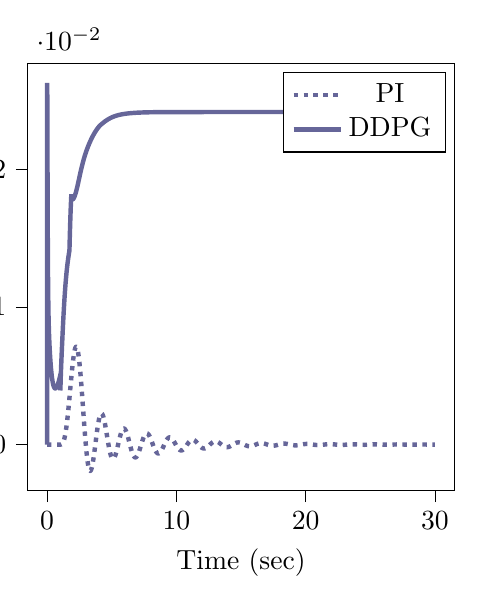
\begin{tikzpicture}[trim axis right,trim axis left]

\definecolor{color0}{rgb}{0.12156862745098,0.466666666666667,0.705882352941177}
\definecolor{color1}{rgb}{1,0.498039215686275,0.0549019607843137}

\begin{axis}[
compat=newest,
tick align=outside,
tick pos=left,
x grid style={white!69.0196078431373!black},
xmin=-1.50000000000009, xmax=31.500000000002,
xtick style={color=black},
y grid style={white!69.0196078431373!black},
ymin=-0.00331591221720112, ymax=0.0276834385040403,
ytick style={color=black},
%yticklabel style={
%        /pgf/number format/.cd,
%        	fixed,
%        	fixed zerofill,
%         	precision=3,
%        /tikz/.cd
%},
scaled y ticks=true,
scaled y ticks=base 10:2,
width=7cm,
height=7cm,
xlabel=Time (sec),
ylabel=Control Signal,
y label style={at={(-0.2,0.5)}}
]
\addplot [ultra thick, blue!20!gray, dotted]
table {%
0 0
0.01 0
0.02 0
0.03 0
0.04 0
0.05 0
0.06 0
0.07 0
0.08 0
0.09 0
0.1 0
0.11 0
0.12 0
0.13 0
0.14 0
0.15 0
0.16 0
0.17 0
0.18 0
0.19 0
0.2 0
0.21 0
0.22 0
0.23 0
0.24 0
0.25 0
0.26 0
0.27 0
0.28 0
0.29 0
0.3 0
0.31 0
0.32 0
0.33 0
0.34 0
0.35 0
0.36 0
0.37 0
0.38 0
0.39 0
0.4 0
0.41 0
0.42 0
0.43 0
0.44 0
0.45 0
0.46 0
0.47 0
0.48 0
0.49 0
0.5 0
0.51 0
0.52 0
0.53 0
0.54 0
0.55 0
0.56 0
0.57 0
0.58 0
0.59 0
0.6 0
0.61 0
0.62 0
0.63 0
0.64 0
0.65 0
0.66 0
0.67 0
0.68 0
0.69 0
0.7 0
0.71 0
0.72 0
0.73 0
0.74 0
0.75 0
0.76 0
0.77 0
0.78 0
0.79 0
0.8 0
0.81 0
0.820000000000001 0
0.830000000000001 0
0.840000000000001 0
0.850000000000001 0
0.860000000000001 0
0.870000000000001 0
0.880000000000001 0
0.890000000000001 0
0.900000000000001 0
0.910000000000001 0
0.920000000000001 0
0.930000000000001 0
0.940000000000001 0
0.950000000000001 0
0.960000000000001 0
0.970000000000001 0
0.980000000000001 0
0.990000000000001 0
1 -4.3927576726343e-19
1.01 6.51165931843092e-09
1.02 6.88168037885038e-08
1.03 2.57142679871956e-07
1.04 6.43147531775966e-07
1.05 1.29756621960344e-06
1.06 2.29157793207718e-06
1.07 3.69658887283981e-06
1.08 5.584093999423e-06
1.09 8.02556017579946e-06
1.1 1.10923121262385e-05
1.11 1.48554134452624e-05
1.12 1.93855436454516e-05
1.13 2.47528721793769e-05
1.14 3.10269302598353e-05
1.15 3.82764812014668e-05
1.16 4.65693899243068e-05
1.17 5.59724921926305e-05
1.18 6.65514641066273e-05
1.19 7.83706923172054e-05
1.2 9.14931453935508e-05
1.21 0.000105980246737521
1.22 0.000121891749407602
1.23 0.000139285613187178
1.24 0.000158217884206755
1.25 0.000178742577407031
1.26 0.000200911562108968
1.27 0.000224774450938019
1.28 0.000250378492332079
1.29 0.000277768466846435
1.3 0.000306986587453742
1.31 0.00033807240402273
1.32 0.000371062712145771
1.33 0.000405991466472624
1.34 0.000442889698695366
1.35 0.000481785440317723
1.36 0.000522703650330712
1.37 0.000565666147905504
1.38 0.000610691550203821
1.39 0.000657795215395797
1.4 0.000706989190965142
1.41 0.000758282167371637
1.42 0.000811679437131271
1.43 0.000867182859364844
1.44 0.000924790829798501
1.45 0.000984498256476486
1.46 0.0010462965408854
1.47 0.00111017356469161
1.48 0.00117611368207008
1.49 0.00124409771757355
1.5 0.0013141029697316
1.51 0.00138610322003686
1.52 0.00146006874751303
1.53 0.00153596634877289
1.54 0.00161375936352312
1.55 0.00169340770546521
1.56 0.00177486789853425
1.57 0.00185809311841062
1.58 0.00194303323923262
1.59 0.00202963488566609
1.6 0.00211784149071758
1.61 0.00220759335694106
1.62 0.00229882772312578
1.63 0.00239147883588126
1.64 0.00248547802593192
1.65 0.0025807537890481
1.66 0.00267723188544788
1.67 0.0027748353965996
1.68 0.00287348482752241
1.69 0.00297309821011458
1.7 0.00307359120393008
1.71 0.00317487720060498
1.72 0.0032768674317769
1.73 0.0033794710803356
1.74 0.00348259539483972
1.75 0.00358614580693015
1.76 0.00369002605156765
1.77 0.00379413828991845
1.78 0.00389838323473531
1.79 0.00400266027798059
1.8 0.00410686762056379
1.81 0.00421090240400543
1.82 0.00431466084382664
1.83 0.00441803836447643
1.84 0.00452092973560502
1.85 0.0046232292094902
1.86 0.00472483065942296
1.87 0.00482562771885778
1.88 0.00492551392113265
1.89 0.00502438283956368
1.9 0.00512212822771936
1.91 0.00521864415967983
1.92 0.00531382517008712
1.93 0.0054075663937933
1.94 0.0054997637049146
1.95 0.00559031385510083
1.96 0.00567911461083126
1.97 0.00576606488954984
1.98 0.00585106489445481
1.99 0.00593401624776022
2 0.00601482212224916
2.01 0.00609338737094173
2.02 0.00616961865470337
2.03 0.00624342456762271
2.04 0.00631471575999138
2.05 0.00638340505872182
2.06 0.00644940758507138
2.07 0.00651264087473041
2.08 0.00657302497693673
2.09 0.00663048257039227
2.1 0.00668493906862615
2.11 0.00673632272189139
2.12 0.00678456471546638
2.13 0.00682959926423663
2.14 0.0068713637034368
2.15 0.00690979857543807
2.16 0.00694484771247119
2.17 0.00697645831518065
2.18 0.00700458102691147
2.19 0.0070291700036354
2.2 0.00705018297942955
2.21 0.00706758132742611
2.22 0.00708133011615843
2.23 0.00709139816123435
2.24 0.00709775807227424
2.25 0.00710038629505759
2.26 0.00709926314882795
2.27 0.00709437285871289
2.28 0.00708570358322166
2.29 0.00707324743678968
2.29999999999999 0.00705700050734544
2.30999999999999 0.00703696286888161
2.31999999999999 0.00701313858901834
2.32999999999999 0.00698553573154843
2.33999999999999 0.00695416635398159
2.34999999999999 0.00691904650006853
2.35999999999999 0.00688019618732991
2.36999999999999 0.00683763939015508
2.37999999999999 0.00679140401686327
2.38999999999999 0.00674152188174172
2.39999999999999 0.0066880286733582
2.40999999999999 0.00663096391740871
2.41999999999999 0.00657037093470004
2.42999999999999 0.00650629679428298
2.43999999999999 0.00643879226173841
2.44999999999999 0.00636791174259503
2.45999999999999 0.00629371326792681
2.46999999999999 0.00621625861761676
2.47999999999999 0.00613561274399405
2.48999999999999 0.00605184398791189
2.49999999999999 0.00596502399992463
2.50999999999999 0.00587522765802701
2.51999999999999 0.00578253298187999
2.52999999999999 0.00568702104352003
2.53999999999999 0.00558877587459342
2.54999999999999 0.00548788437018674
2.55999999999999 0.00538443618934432
2.56999999999999 0.00527852365237848
2.57999999999999 0.0051702416350889
2.58999999999999 0.00505968746001577
2.59999999999999 0.00494696078485864
2.60999999999999 0.00483216348819829
2.61999999999999 0.00471539955266385
2.62999999999999 0.00459677494569157
2.63999999999999 0.00447639749802542
2.64999999999999 0.00435437678011289
2.65999999999999 0.00423082397655175
2.66999999999999 0.00410585175874703
2.67999999999999 0.00397957415593846
2.68999999999999 0.00385210642476167
2.69999999999999 0.00372356491750706
2.70999999999999 0.00359406694924249
2.71999999999999 0.00346373066396653
2.72999999999999 0.00333267489995996
2.73999999999999 0.00320101905450428
2.74999999999999 0.00306888294813569
2.75999999999999 0.00293638668860385
2.76999999999998 0.00280365053470432
2.77999999999998 0.00267079476015323
2.78999999999998 0.00253793951767278
2.79999999999998 0.00240520470345469
2.80999999999998 0.0022727098221684
2.81999999999998 0.0021405738526793
2.82999999999998 0.0020089151146414
2.83999999999998 0.00187785113612658
2.84999999999998 0.00174749852245142
2.85999999999998 0.0016179728263604
2.86999999999998 0.00148938841972212
2.87999999999998 0.00136185836689281
2.88999999999998 0.00123549429989886
2.89999999999998 0.00111040629558756
2.90999999999998 0.000986702754897498
2.91999999999998 0.000864490284394157
2.92999999999998 0.000743873580147423
2.93999999999998 0.00062495531420673
2.94999999999998 0.000507836023720285
2.95999999999998 0.000392614002849654
2.96999999999998 0.000279385197604974
2.97999999999998 0.000168243103721868
2.98999999999998 5.92786676971333e-05
2.99999999999998 -4.74198089041051e-05
3.00999999999998 -0.000151766761761477
3.01999999999998 -0.00025367945262902
3.02999999999998 -0.000353078054582202
3.03999999999998 -0.000449885733587982
3.04999999999998 -0.000544028726308518
3.05999999999998 -0.000635436414053836
3.06999999999998 -0.000724041392803974
3.07999999999998 -0.000809779539226145
3.08999999999998 -0.000892590072617571
3.09999999999998 -0.000972415612700121
3.10999999999998 -0.00104920223324566
3.11999999999998 -0.00112289951144076
3.12999999999998 -0.00119346057292027
3.13999999999998 -0.00126084213248062
3.14999999999998 -0.00132500453041183
3.15999999999998 -0.00138591176441535
3.16999999999998 -0.00144353151722942
3.17999999999998 -0.00149783518017011
3.18999999999998 -0.00154879787005109
3.19999999999998 -0.00159639844411324
3.20999999999998 -0.00164061950953295
3.21999999999998 -0.00168144742840524
3.22999999999998 -0.00171887231819065
3.23999999999997 -0.00175288804761336
3.24999999999997 -0.00178349222799154
3.25999999999997 -0.0018106861999693
3.26999999999997 -0.00183447501559835
3.27999999999997 -0.00185486741568077
3.28999999999997 -0.0018718758022218
3.29999999999997 -0.00188551620573351
3.30999999999997 -0.00189580931544134
3.31999999999997 -0.00190277768604433
3.32999999999997 -0.00190644810017757
3.33999999999997 -0.00190685082078106
3.34999999999997 -0.00190401954193931
3.35999999999997 -0.00189799133713649
3.36999999999997 -0.00188880660618272
3.37999999999997 -0.00187650902358327
3.38999999999997 -0.00186114550550286
3.39999999999997 -0.00184276568571318
3.40999999999997 -0.00182142246932561
3.41999999999997 -0.00179717180542219
3.42999999999997 -0.00177007253959398
3.43999999999997 -0.00174018633193757
3.44999999999997 -0.00170757757207629
3.45999999999997 -0.00167231329131423
3.46999999999997 -0.00163446307203615
3.47999999999997 -0.00159409888467813
3.48999999999997 -0.00155129498481572
3.49999999999997 -0.00150612808134272
3.50999999999997 -0.00145867703047713
3.51999999999997 -0.00140902274166476
3.52999999999997 -0.00135724807672237
3.53999999999997 -0.00130343774517851
3.54999999999997 -0.00124767819701319
3.55999999999997 -0.00119005751337967
3.56999999999997 -0.00113066529565068
3.57999999999997 -0.00106959255302818
3.58999999999997 -0.00100693005397189
3.59999999999997 -0.000942773105068836
3.60999999999997 -0.000877216209631927
3.61999999999997 -0.000810354825441027
3.62999999999997 -0.00074228524637907
3.63999999999997 -0.000673104483918077
3.64999999999997 -0.000602910148517982
3.65999999999997 -0.000531800331025578
3.66999999999997 -0.000459873484176939
3.67999999999997 -0.000387228304317299
3.68999999999997 -0.000313963613459522
3.69999999999997 -0.000240178241808913
3.70999999999996 -0.000165970910878039
3.71999999999996 -9.14401173227679e-05
3.72999999999996 -1.66840176338577e-05
3.73999999999996 5.81996861869997e-05
3.74999999999996 0.00013311385983626
3.75999999999996 0.000207962048673402
3.76999999999996 0.000282648588313445
3.77999999999996 0.000357078713720786
3.78999999999996 0.000431158666679813
3.79999999999996 0.000504795801519935
3.80999999999996 0.000577898688975066
3.81999999999996 0.000650377218060189
3.82999999999996 0.000722142695889003
3.83999999999996 0.000793107945187091
3.84999999999996 0.000863187399531708
3.85999999999996 0.00093229719621012
3.86999999999996 0.00100035526652126
3.87999999999996 0.00106728142345293
3.88999999999996 0.00113299744663936
3.89999999999996 0.00119742716450776
3.90999999999996 0.00126049653352611
3.91999999999996 0.00132213371446853
3.92999999999996 0.0013822691456183
3.93999999999996 0.00144083561283274
3.94999999999996 0.00149776831639835
3.95999999999996 0.00155300493460856
3.96999999999996 0.00160648568400082
3.97999999999996 0.00165815337619379
3.98999999999996 0.00170795347126981
3.99999999999996 0.00175583412765186
4.00999999999996 0.0018017462484285
4.01999999999996 0.00184564352408424
4.02999999999996 0.00188748247159704
4.03999999999996 0.00192722246986788
4.04999999999996 0.00196482579145146
4.05999999999996 0.00200025763059678
4.06999999999996 0.00203348612843875
4.07999999999996 0.00206448239141095
4.08999999999996 0.00209322050898761
4.09999999999996 0.00211967758471578
4.10999999999996 0.00214383384217253
4.11999999999996 0.00216567239900753
4.12999999999996 0.00218517938890401
4.13999999999996 0.00220234395989691
4.14999999999996 0.00221715826903158
4.15999999999996 0.00222961747339494
4.16999999999996 0.00223971971756126
4.17999999999996 0.00224746611751002
4.18999999999996 0.00225286074109805
4.19999999999995 0.00225591058521286
4.20999999999995 0.00225662554982292
4.21999999999995 0.00225501841023307
4.22999999999995 0.00225110478494982
4.23999999999995 0.00224490310607931
4.24999999999995 0.00223643459499029
4.25999999999995 0.00222572286926878
4.26999999999995 0.00221279440842352
4.27999999999995 0.00219767839059988
4.28999999999995 0.00218040655597345
4.29999999999995 0.00216101315499718
4.30999999999995 0.00213953489203037
4.31999999999995 0.00211601086542408
4.32999999999995 0.00209048250457282
4.33999999999995 0.00206299350421918
4.34999999999995 0.00203358975620237
4.35999999999995 0.00200231927879811
4.36999999999995 0.00196923214377681
4.37999999999995 0.0019343804012975
4.38999999999995 0.00189781800275036
4.39999999999995 0.00185960072165951
4.40999999999995 0.00181978607275689
4.41999999999995 0.00177843322933907
4.42999999999995 0.0017356029390193
4.43999999999995 0.00169135743798831
4.44999999999995 0.00164576036389831
4.45999999999995 0.00159887666748558
4.46999999999995 0.00155077133842975
4.47999999999995 0.00150151299806922
4.48999999999995 0.00145116998134318
4.49999999999995 0.0013998115740688
4.50999999999995 0.00134750791979499
4.51999999999995 0.00129432992603328
4.52999999999995 0.00124034917032461
4.53999999999995 0.00118563780589199
4.54999999999995 0.00113026846711211
4.55999999999995 0.00107431417492269
4.56999999999995 0.0010178482422817
4.57999999999995 0.000960944179794845
4.58999999999995 0.000903675601626453
4.59999999999995 0.000846116131808848
4.60999999999995 0.000788339311063952
4.61999999999995 0.00073041850424989
4.62999999999995 0.000672426808544472
4.63999999999995 0.000614436962475647
4.64999999999995 0.000556521255907823
4.65999999999995 0.000498751441091128
4.66999999999994 0.000441198644879147
4.67999999999994 0.000383933282218462
4.68999999999994 0.000327024971011616
4.69999999999994 0.000270542448456266
4.70999999999994 0.000214553488950477
4.71999999999994 0.000159124823652942
4.72999999999994 0.00010432206181466
4.73999999999994 5.02096139513599e-05
4.74999999999994 -3.14938305113241e-06
4.75999999999994 -5.56931380565489e-05
4.76999999999994 -0.000107361272155847
4.77999999999994 -0.000158094899040353
4.78999999999994 -0.000207836684572148
4.79999999999994 -0.000256530910834074
4.80999999999994 -0.000304123537785906
4.81999999999994 -0.000350562262461688
4.82999999999994 -0.000395796575646166
4.83999999999994 -0.000439777815971676
4.84999999999994 -0.000482459221408591
4.85999999999994 -0.00052379597803319
4.86999999999994 -0.000563745265975748
4.87999999999994 -0.000602266302751015
4.88999999999994 -0.000639320004224856
4.89999999999994 -0.000674870257107564
4.90999999999994 -0.000708882621370187
4.91999999999994 -0.000741324840472462
4.92999999999994 -0.000772166870166031
4.93999999999994 -0.000801380904354541
4.94999999999994 -0.000828941397991575
4.95999999999994 -0.000854825087001539
4.96999999999994 -0.000879011006129877
4.97999999999994 -0.000901480501009033
4.98999999999994 -0.000922217239996031
4.99999999999994 -0.000941207222168692
5.00999999999994 -0.000958438782285843
5.01999999999994 -0.000973902592772246
5.02999999999994 -0.000987591662742295
5.03999999999994 -0.000999501334086339
5.04999999999994 -0.0010096292746512
5.05999999999994 -0.00101797546855662
5.06999999999994 -0.00102454220370637
5.07999999999994 -0.00102933405657978
5.08999999999994 -0.00103235787484939
5.09999999999994 -0.00103362275708039
5.10999999999994 -0.00103314002978099
5.11999999999994 -0.00103092322484262
5.12999999999994 -0.00102698805725571
5.13999999999993 -0.00102135240857475
5.14999999999993 -0.00101403633027024
5.15999999999993 -0.00100506157143968
5.16999999999993 -0.000994452002197018
5.17999999999993 -0.000982233604141436
5.18999999999993 -0.000968434218470915
5.19999999999993 -0.000953083526118324
5.20999999999993 -0.000936213268075238
5.21999999999993 -0.000917856944126288
5.22999999999993 -0.000898049778984971
5.23999999999993 -0.000876828675880681
5.24999999999993 -0.000854232164064432
5.25999999999993 -0.000830300342652613
5.26999999999993 -0.000805074821856125
5.27999999999993 -0.000778598662116011
5.28999999999993 -0.0007509163114444
5.29999999999993 -0.000722073541168671
5.30999999999993 -0.000692117380227792
5.31999999999993 -0.00066109604814543
5.32999999999993 -0.000629058886791364
5.33999999999993 -0.000596056291035962
5.34999999999993 -0.000562139638398915
5.35999999999993 -0.000527361217791289
5.36999999999993 -0.000491774157449087
5.37999999999993 -0.000455432352155878
5.38999999999993 -0.000418390389851839
5.39999999999993 -0.000380703477726443
5.40999999999993 -0.000342427367891833
5.41999999999993 -0.000303618282733829
5.42999999999993 -0.000264332840037299
5.43999999999993 -0.000224627977982316
5.44999999999993 -0.000184560880107265
5.45999999999993 -0.000144188900334443
5.46999999999993 -0.000103569488153246
5.47999999999993 -6.27601140552497e-05
5.48999999999993 -2.18181953174986e-05
5.49999999999993 1.91989777805952e-05
5.50999999999993 6.02343152104784e-05
5.51999999999993 0.000101230999824659
5.52999999999993 0.000142132559277971
5.53999999999993 0.000182882937151174
5.54999999999993 0.000223426563190206
5.55999999999993 0.000263708422576222
5.56999999999993 0.00030367412414288
5.57999999999993 0.000343269967459302
5.58999999999993 0.000382443008698875
5.59999999999993 0.000421141125215975
5.60999999999992 0.000459313078754736
5.61999999999992 0.00049690857721606
5.62999999999992 0.000533878334911257
5.63999999999992 0.000570174131232952
5.64999999999992 0.000605748867676303
5.65999999999992 0.000640556623145826
5.66999999999992 0.00067455270748582
5.67999999999992 0.000707693713174787
5.68999999999992 0.00073993756512688
5.69999999999992 0.000771243568546151
5.70999999999992 0.000801572454782016
5.71999999999992 0.000830886425137261
5.72999999999992 0.000859149192582599
5.73999999999992 0.000886326021334829
5.74999999999992 0.000912383764258455
5.75999999999992 0.000937290898053686
5.76999999999992 0.000961017556196665
5.77999999999992 0.000983535559600959
5.78999999999992 0.00100481844497224
5.79999999999992 0.00102484149083145
5.80999999999992 0.00104358174118469
5.81999999999992 0.00106101802753849
5.82999999999992 0.0010771309866893
5.83999999999992 0.00109190307723672
5.84999999999992 0.00110531859408056
5.85999999999992 0.00111736368011865
5.86999999999992 0.00112802633553383
5.87999999999992 0.00113729642467469
5.88999999999992 0.00114516568054071
5.89999999999992 0.00115162770688973
5.90999999999992 0.00115667797799711
5.91999999999992 0.0011603138361121
5.92999999999992 0.00116253448668561
5.93999999999992 0.00116334099149402
5.94999999999992 0.00116273625988244
5.95999999999992 0.001160725038556
5.96999999999992 0.0011573139008095
5.97999999999992 0.00115251123722857
5.98999999999992 0.00114632725302703
5.99999999999992 0.00113877398292089
6.00999999999992 0.00112986522742565
6.01999999999992 0.00111961581796481
6.02999999999992 0.00110804276953544
6.03999999999992 0.00109516475487291
6.04999999999992 0.00108100207257312
6.05999999999992 0.00106557661333116
6.06999999999992 0.00104891182425416
6.07999999999991 0.00103103257134074
6.08999999999991 0.0010119651576257
6.09999999999991 0.0009917375649034
6.10999999999991 0.000970379130114412
6.11999999999991 0.000947920521468604
6.12999999999991 0.000924393702352676
6.13999999999991 0.000899831889218375
6.14999999999991 0.000874269505925382
6.15999999999991 0.000847742135658953
6.16999999999991 0.000820286470991603
6.17999999999991 0.000791940262413891
6.18999999999991 0.000762742265543077
6.19999999999991 0.000732732185874542
6.20999999999991 0.000701950625383575
6.21999999999991 0.000670439027535378
6.22999999999991 0.000638239619079793
6.23999999999991 0.000605395352480285
6.24999999999991 0.000571949847650462
6.25999999999991 0.000537947333082864
6.26999999999991 0.000503432586452664
6.27999999999991 0.000468450874777746
6.28999999999991 0.000433047894215704
6.29999999999991 0.000397269709577696
6.30999999999991 0.000361162693638737
6.31999999999991 0.000324773466323368
6.32999999999991 0.00028814883384543
6.33999999999991 0.000251335727880021
6.34999999999991 0.000214381144845327
6.35999999999991 0.000177332085371417
6.36999999999991 0.000140235494032275
6.37999999999991 0.000103138199420407
6.38999999999991 6.60868546273609e-05
6.39999999999991 2.91278782166639e-05
6.40999999999991 -7.69260424183745e-06
6.41999999999991 -4.43288180054996e-05
6.42999999999991 -8.0737518974195e-05
6.43999999999991 -0.000116871776915786
6.44999999999991 -0.000152687209045219
6.45999999999991 -0.000188140005100654
6.46999999999991 -0.000223186981099874
6.47999999999991 -0.000257785632045113
6.48999999999991 -0.000291894183515762
6.49999999999991 -0.000325471642089776
6.50999999999991 -0.000358477844536155
6.51999999999991 -0.000390873505722421
6.52999999999991 -0.000422620265182755
6.53999999999991 -0.00045368073229404
6.5499999999999 -0.000484018530009089
6.5599999999999 -0.000513598337098017
6.5699999999999 -0.000542383014896397
6.5799999999999 -0.000570342430823082
6.5899999999999 -0.000597444684929147
6.5999999999999 -0.000623659087769146
6.6099999999999 -0.000648956194463405
6.6199999999999 -0.000673307837033337
6.6299999999999 -0.000696687154975508
6.6399999999999 -0.000719068624042821
6.6499999999999 -0.000740428083203709
6.6599999999999 -0.000760742759752735
6.6699999999999 -0.000779991292548694
6.6799999999999 -0.000798153753358845
6.6899999999999 -0.00081521166629057
6.6999999999999 -0.000831148025294513
6.7099999999999 -0.000845947310385325
6.7199999999999 -0.000859595500241081
6.7299999999999 -0.000872080083798817
6.7399999999999 -0.000883390070331681
6.7499999999999 -0.0008935159971717
6.7599999999999 -0.000902449935470658
6.7699999999999 -0.000910185494006413
6.7799999999999 -0.000916717821047698
6.7899999999999 -0.000922043604297847
6.7999999999999 -0.000926161068948769
6.8099999999999 -0.000929069973893019
6.8199999999999 -0.000930771606168833
6.8299999999999 -0.000931268773763252
6.8399999999999 -0.000930565796985264
6.8499999999999 -0.000928668498802934
6.8599999999999 -0.000925584194922016
6.8699999999999 -0.00092132168526862
6.8799999999999 -0.000915891249154558
6.8899999999999 -0.000909304611441432
6.8999999999999 -0.00090157493735924
6.9099999999999 -0.000892716453742649
6.9199999999999 -0.000882744769740168
6.9299999999999 -0.000871677020622556
6.9399999999999 -0.000859531655350611
6.9499999999999 -0.000846328407488606
6.9599999999999 -0.000832088264657493
6.9699999999999 -0.000816833237685479
6.9799999999999 -0.000800586673674915
6.9899999999999 -0.000783373190023493
6.9999999999999 -0.000765218521541429
7.00999999999989 -0.000746149460065306
7.01999999999989 -0.000726193825970503
7.02999999999989 -0.000705380434029113
7.03999999999989 -0.00068373905580009
7.04999999999989 -0.000661300379749047
7.05999999999989 -0.000638095969705484
7.06999999999989 -0.000614158221999586
7.07999999999989 -0.0005895203214924
7.08999999999989 -0.000564216196647835
7.09999999999989 -0.000538280473759659
7.10999999999989 -0.000511748430427448
7.11999999999989 -0.00048465594836397
7.12999999999989 -0.000457039465610106
7.13999999999989 -0.000428935928229273
7.14999999999989 -0.000400382741550813
7.15999999999989 -0.0003714177210304
7.16999999999989 -0.000342079042794242
7.17999999999989 -0.000312405193933345
7.18999999999989 -0.000282434922613374
7.19999999999989 -0.000252207188065278
7.20999999999989 -0.000221761110521385
7.21999999999989 -0.000191135921159048
7.22999999999989 -0.000160370912115443
7.23999999999989 -0.00012950538665105
7.24999999999989 -9.85786095060889e-05
7.25999999999989 -6.7629757518765e-05
7.26999999999989 -3.66978705700653e-05
7.27999999999989 -5.82001171819669e-06
7.28999999999989 2.49635407144578e-05
7.29999999999989 5.56144495473391e-05
7.30999999999989 8.60947044008799e-05
7.31999999999989 0.000116366668359133
7.32999999999989 0.000146393123943096
7.33999999999989 0.00017613731834166
7.34999999999989 0.000205563007847536
7.35999999999989 0.000234634501446879
7.36999999999989 0.000263316703512158
7.37999999999989 0.000291575155450231
7.38999999999989 0.00031937607648496
7.39999999999989 0.000346686403575021
7.40999999999989 0.000373473829904068
7.41999999999989 0.000399706842376132
7.42999999999989 0.000425354757938294
7.43999999999989 0.000450387758689532
7.44999999999989 0.000474776925736196
7.45999999999989 0.000498491235157021
7.46999999999989 0.000521506744269154
7.47999999999988 0.000543797442180646
7.48999999999988 0.000565338340641269
7.49999999999988 0.000586105501095078
7.50999999999988 0.000606076060294338
7.51999999999988 0.000625228254448438
7.52999999999988 0.000643541441883425
7.53999999999988 0.000660996124189963
7.54999999999988 0.000677573965839678
7.55999999999988 0.00069325781236641
7.56999999999988 0.000708031706620531
7.57999999999988 0.000721880903755601
7.58999999999988 0.00073479188537712
7.59999999999988 0.000746752369900651
7.60999999999988 0.000757751323101262
7.61999999999988 0.000767778966829675
7.62999999999988 0.000776826785929624
7.63999999999988 0.000784887533553268
7.64999999999988 0.000791955234884144
7.65999999999988 0.000798025189283944
7.66999999999988 0.00080309397088899
7.67999999999988 0.000807159427697048
7.68999999999988 0.000810220679208747
7.69999999999988 0.000812278112728514
7.70999999999988 0.00081333337850332
7.71999999999988 0.000813389384017868
7.72999999999988 0.000812450288053412
7.73999999999988 0.000810521489949887
7.74999999999988 0.000807609611508065
7.75999999999988 0.000803722493507435
7.76999999999988 0.000798869190549301
7.77999999999988 0.000793059970973194
7.78999999999988 0.00078630576743738
7.79999999999988 0.000778619020172148
7.80999999999988 0.000770013288159776
7.81999999999988 0.000760503226861238
7.82999999999988 0.000750104564708008
7.83999999999988 0.000738834078385235
7.84999999999988 0.00072670956693569
7.85999999999988 0.000713749583113468
7.86999999999988 0.000699973935897631
7.87999999999988 0.000685403360498981
7.88999999999988 0.000670059490887449
7.89999999999988 0.000653964844043959
7.90999999999988 0.000637142776776137
7.91999999999988 0.000619617448332432
7.92999999999988 0.000601413789366157
7.93999999999988 0.000582557468920349
7.94999999999987 0.000563074859980503
7.95999999999987 0.000542993003907879
7.96999999999987 0.000522339573949935
7.97999999999987 0.000501142837963488
7.98999999999987 0.000479431620452833
7.99999999999987 0.000457235264006297
8.00999999999987 0.000434583590203277
8.01999999999987 0.000411506860057427
8.02999999999987 0.00038803573405719
8.03999999999987 0.000364201231862421
8.04999999999987 0.000340034691714031
8.05999999999987 0.000315567729612398
8.06999999999987 0.000290832198319488
8.07999999999987 0.000265860146238804
8.08999999999987 0.000240683776227219
8.09999999999987 0.000215335404391568
8.10999999999987 0.000189847418923089
8.11999999999987 0.000164252239021999
8.12999999999987 0.000138582273964022
8.13999999999987 0.000112868462392435
8.14999999999987 8.7144327899443e-05
8.15999999999987 6.14420028545988e-05
8.16999999999987 3.57934503952166e-05
8.17999999999987 1.0230424840906e-05
8.18999999999987 -1.52155674362094e-05
8.19999999999987 -4.05133066403858e-05
8.20999999999987 -6.56318976355855e-05
8.21999999999987 -9.05408074391579e-05
8.22999999999987 -0.000115209902082366
8.23999999999987 -0.000139609482795208
8.24999999999987 -0.000163710321473577
8.25999999999987 -0.000187483695387855
8.26999999999987 -0.000210901421093137
8.27999999999987 -0.000233935887474376
8.28999999999987 -0.000256560087800094
8.29999999999987 -0.000278747651354379
8.30999999999987 -0.000300472873601856
8.31999999999987 -0.000321710745544478
8.32999999999987 -0.000342436982063528
8.33999999999987 -0.000362628049215174
8.34999999999987 -0.000382261190448976
8.35999999999987 -0.000401314451720089
8.36999999999987 -0.000419766705466999
8.37999999999987 -0.000437594565322085
8.38999999999987 -0.000454781822508391
8.39999999999987 -0.000471309988040943
8.40999999999987 -0.000487161484862129
8.41999999999986 -0.000502319665851657
8.42999999999986 -0.000516768830585999
8.43999999999986 -0.000530494240832151
8.44999999999986 -0.000543482134762364
8.45999999999986 -0.000555719739878455
8.46999999999986 -0.000567195284977926
8.47999999999986 -0.000577898010217318
8.48999999999986 -0.00058781817553063
8.49999999999986 -0.000596947068808741
8.50999999999986 -0.000605277012277963
8.51999999999986 -0.000612801367569032
8.52999999999986 -0.000619514539485376
8.53999999999986 -0.000625411978485807
8.54999999999986 -0.000630490181905725
8.55999999999986 -0.000634746693954546
8.56999999999986 -0.00063818010454902
8.57999999999986 -0.000640790047078914
8.58999999999986 -0.00064257719526727
8.59999999999986 -0.000643543257127718
8.60999999999986 -0.000643690966088981
8.61999999999986 -0.000643024075748282
8.62999999999986 -0.000641547352454532
8.63999999999986 -0.000639266567973389
8.64999999999986 -0.000636188493722351
8.65999999999986 -0.000632320900809666
8.66999999999986 -0.00062767231945417
8.67999999999986 -0.000622252179122643
8.68999999999986 -0.000616070988449339
8.69999999999986 -0.000609140166106649
8.70999999999986 -0.000601472022033637
8.71999999999986 -0.000593079737665097
8.72999999999986 -0.000583977345183755
8.73999999999986 -0.000574179705820694
8.74999999999986 -0.000563702304312367
8.75999999999986 -0.000552561615708362
8.76999999999986 -0.000540774877753776
8.77999999999986 -0.000528360054196516
8.78999999999986 -0.00051533581140106
8.79999999999986 -0.000501721493073425
8.80999999999986 -0.000487537093674446
8.81999999999986 -0.000472803233384314
8.82999999999986 -0.000457541130533917
8.83999999999986 -0.000441772567119649
8.84999999999986 -0.000425519859052948
8.85999999999986 -0.000408805826240352
8.86999999999986 -0.000391653761969027
8.87999999999986 -0.000374087401705414
8.88999999999985 -0.000356130891390453
8.89999999999985 -0.0003378087553003
8.90999999999985 -0.00031914586353264
8.91999999999985 -0.000300167399173401
8.92999999999985 -0.000280898825194959
8.93999999999985 -0.000261365851134712
8.94999999999985 -0.000241594399601246
8.95999999999985 -0.000221610572654195
8.96999999999985 -0.000201440618103103
8.97999999999985 -0.000181110895769825
8.98999999999985 -0.000160647843758595
8.99999999999985 -0.000140077944777109
9.00999999999985 -0.000119427692551848
9.01999999999985 -9.87235583803074e-05
9.02999999999985 -7.79906480720846e-05
9.03999999999985 -5.7256425282872e-05
9.04999999999985 -3.65470930131651e-05
9.05999999999985 -1.58887021304518e-05
9.06999999999985 4.69288088570665e-06
9.07999999999985 2.51720058045781e-05
9.08999999999985 4.55232700746239e-05
9.09999999999985 6.57215497873146e-05
9.10999999999985 8.57420301387419e-05
9.11999999999985 0.00010556023535397
9.12999999999985 0.000125152058039655
9.13999999999985 0.000144493787931155
9.14999999999985 0.000163562140001165
9.15999999999985 0.000182334281897641
9.16999999999985 0.000200787860541249
9.17999999999985 0.000218901028347084
9.18999999999985 0.000236652468423627
9.19999999999985 0.0002540214189856
9.20999999999985 0.000270987696985738
9.21999999999985 0.000287531720901533
9.22999999999985 0.000303634532651297
9.23999999999985 0.000319277818614868
9.24999999999985 0.000334443929735309
9.25999999999985 0.000349112928559157
9.26999999999985 0.000363271593135913
9.27999999999985 0.000376904406623755
9.28999999999985 0.000389996588753379
9.29999999999985 0.000402534111105128
9.30999999999985 0.000414503711368149
9.31999999999985 0.000425892906568844
9.32999999999985 0.000436690005257449
9.33999999999985 0.000446884118643201
9.34999999999985 0.000456465170727281
9.35999999999984 0.000465423907779174
9.36999999999984 0.000473751905121898
9.37999999999984 0.000481441574625354
9.38999999999984 0.000488486170506872
9.39999999999984 0.000494879794065599
9.40999999999984 0.000500617397359133
9.41999999999984 0.000505694785836645
9.42999999999984 0.000510108619951028
9.43999999999984 0.000513856415771249
9.44999999999984 0.000516936543756351
9.45999999999984 0.000519348226681352
9.46999999999984 0.000521091537110691
9.47999999999984 0.000522167393766589
9.48999999999984 0.000522577557010436
9.49999999999984 0.000522324623551474
9.50999999999984 0.000521412020584409
9.51999999999984 0.000519843999747797
9.52999999999984 0.000517625631737965
9.53999999999984 0.000514762803729688
9.54999999999984 0.000511262173817611
9.55999999999984 0.000507130906933957
9.56999999999984 0.00050237715601023
9.57999999999984 0.000497009824623378
9.58999999999984 0.00049103855207422
9.59999999999984 0.000484473697639623
9.60999999999984 0.000477326324016009
9.61999999999984 0.000469608179973957
9.62999999999984 0.000461331576032831
9.63999999999984 0.000452509543717814
9.64999999999984 0.000443155804801596
9.65999999999984 0.000433284683194432
9.66999999999984 0.000422911086683687
9.67999999999984 0.000412050486848568
9.68999999999984 0.00040071889776643
9.69999999999984 0.000388932853811973
9.70999999999984 0.000376709386716464
9.71999999999984 0.000364066001991814
9.72999999999984 0.00035102065479318
9.73999999999984 0.000337591725360972
9.74999999999984 0.000323797995733857
9.75999999999984 0.000309658622458662
9.76999999999984 0.000295193109864874
9.77999999999984 0.000280421284024876
9.78999999999984 0.000265363266374922
9.79999999999984 0.000250039447045846
9.80999999999984 0.000234470457948399
9.81999999999984 0.000218677145655244
9.82999999999983 0.000202680544119826
9.83999999999983 0.000186501847270987
9.84999999999983 0.000170162381521314
9.85999999999983 0.00015368357822631
9.86999999999983 0.000137086946045393
9.87999999999983 0.000120394043469399
9.88999999999983 0.000103626451528469
9.89999999999983 8.68057462599968e-05
9.90999999999983 6.99534714630358e-05
9.91999999999983 5.30911116141907e-05
9.92999999999983 3.62387060330179e-05
9.93999999999983 1.94187253799691e-05
9.94999999999983 2.65231664988914e-06
9.95999999999983 -1.40395368649848e-05
9.96999999999983 -3.06360414284512e-05
9.97999999999983 -4.71166183454376e-05
9.98999999999983 -6.34609290495802e-05
9.99999999999983 -7.964889976446e-05
10.0099999999998 -9.56607457102827e-05
10.0199999999998 -0.000111476994827946
10.0299999999998 -0.000127078510993448
10.0399999999998 -0.000142446516695849
10.0499999999998 -0.00015756261509766
10.0599999999998 -0.00017240881157533
10.0699999999998 -0.000186967534758854
10.0799999999998 -0.000201221656730533
10.0899999999998 -0.000215154512645181
10.0999999999998 -0.000228749919668896
10.1099999999998 -0.000241992195214833
10.1199999999998 -0.000254863351862101
10.1299999999998 -0.000267351597149971
10.1399999999998 -0.000279442876254378
10.1499999999998 -0.000291123701108601
10.1599999999998 -0.000302381164893086
10.1699999999998 -0.000313202955723211
10.1799999999998 -0.000323577369521979
10.1899999999998 -0.000333493322065881
10.1999999999998 -0.000342940360193277
10.2099999999998 -0.000351908672166025
10.2199999999998 -0.000360389097176292
10.2299999999998 -0.000368373133992056
10.2399999999998 -0.00037585294908076
10.2499999999998 -0.000382821382958865
10.2599999999998 -0.000389271956271507
10.2699999999998 -0.000395198875130496
10.2799999999998 -0.000400597035413581
10.2899999999998 -0.000405462025923608
10.2999999999998 -0.000409790130741297
10.3099999999998 -0.000413578330814968
10.3199999999998 -0.00041682430467916
10.3299999999998 -0.000419526428312231
10.3399999999998 -0.000421683774147435
10.3499999999998 -0.000423296109258454
10.3599999999998 -0.000424363892750419
10.3699999999998 -0.000424888272404212
10.3799999999998 -0.000424871080652386
10.3899999999998 -0.000424314830021245
10.3999999999998 -0.00042322270829292
10.4099999999998 -0.000421598573909095
10.4199999999998 -0.000419446952820644
10.4299999999998 -0.000416773040375553
10.4399999999998 -0.000413582453551226
10.4499999999998 -0.000409881539522336
10.4599999999998 -0.000405677309764068
10.4699999999998 -0.000400977381661156
10.4799999999998 -0.000395789965951871
10.4899999999998 -0.000390123853503803
10.4999999999998 -0.000383988401436961
10.5099999999998 -0.000377393518611267
10.5199999999998 -0.000370349518175526
10.5299999999998 -0.000362867392387164
10.5399999999998 -0.00035495863136209
10.5499999999998 -0.000346635208074377
10.5599999999998 -0.000337909562708243
10.5699999999998 -0.000328794585760155
10.5799999999998 -0.000319303600268504
10.5899999999998 -0.000309450343365207
10.5999999999998 -0.000299248947262535
10.6099999999998 -0.000288713919749524
10.6199999999998 -0.000277860124252442
10.6299999999998 -0.000266702759503227
10.6399999999998 -0.000255257338853743
10.6499999999998 -0.000243539669270443
10.6599999999998 -0.000231565829919811
10.6699999999998 -0.000219352150765011
10.6799999999998 -0.000206915190902497
10.6899999999998 -0.00019427171645491
10.6999999999998 -0.000181438678475361
10.7099999999998 -0.00016843319112743
10.7199999999998 -0.000155272508792692
10.7299999999998 -0.00014197400345371
10.7399999999998 -0.000128555142230988
10.7499999999998 -0.000115033464893068
10.7599999999998 -0.000101426561370291
10.7699999999998 -8.77520493017954e-05
10.7799999999998 -7.40275516452067e-05
10.7899999999998 -6.02706743779184e-05
10.7999999999998 -4.6498984318326e-05
10.8099999999998 -3.27299870943226e-05
10.8199999999998 -1.89811052881049e-05
10.8299999999998 -5.26965678355284e-06
10.8399999999998 8.38867648610009e-06
10.8499999999998 2.19754998038374e-05
10.8599999999998 3.54739320882484e-05
10.8699999999998 4.88672796249112e-05
10.8799999999998 6.21390563718082e-05
10.8899999999998 7.52730039028754e-05
10.8999999999998 8.82531109667092e-05
10.9099999999998 0.000101063632638033
10.9199999999998 0.00011368910903986
10.9299999999998 0.000126114383596082
10.9399999999998 0.000138324620766731
10.9499999999998 0.00015030532352701
10.9599999999998 0.000162042350075052
10.9699999999998 0.000173519407206441
10.9799999999998 0.000184725595541076
10.9899999999998 0.000195647955099068
10.9999999999998 0.00020627394369705
11.0099999999998 0.000216591450939308
11.0199999999998 0.000226588811597533
11.0299999999998 0.00023625481836555
11.0399999999998 0.000245578733976364
11.0499999999998 0.000254550302669571
11.0599999999998 0.000263159760998297
11.0699999999998 0.000271397847965665
11.0799999999998 0.000279255814565155
11.0899999999998 0.000286725432537443
11.0999999999998 0.000293799002296601
11.1099999999998 0.000300469360281673
11.1199999999998 0.000306729885697886
11.1299999999998 0.000312574506518572
11.1399999999998 0.000317997704210236
11.1499999999998 0.000322994518522197
11.1599999999998 0.000327560551251689
11.1699999999998 0.00033169196928639
11.1799999999998 0.000335385506925691
11.1899999999998 0.00033863846748352
11.1999999999998 0.000341448724177477
11.2099999999998 0.000343814720311429
11.2199999999998 0.000345735468761929
11.2299999999998 0.000347210550767423
11.2399999999998 0.00034824011399644
11.2499999999998 0.000348824870190953
11.2599999999998 0.000348966092057585
11.2699999999998 0.000348665609718026
11.2799999999998 0.000347925806830119
11.2899999999998 0.000346749616693737
11.2999999999998 0.000345140519029529
11.3099999999998 0.000343102539231469
11.3199999999998 0.000340640156811537
11.3299999999998 0.000337758280220572
11.3399999999998 0.000334462438358695
11.3499999999998 0.000330758659443635
11.3599999999998 0.000326653460988978
11.3699999999998 0.000322153839230542
11.3799999999998 0.000317267258013242
11.3899999999998 0.000312001637151941
11.3999999999998 0.000306365278409416
11.4099999999998 0.000300366941069578
11.4199999999998 0.000294015856629991
11.4299999999998 0.000287321655940409
11.4399999999998 0.000280294357110507
11.4499999999998 0.000272944352129318
11.4599999999998 0.000265282392645924
11.4699999999998 0.000257319575130028
11.4799999999998 0.000249067325527898
11.4899999999998 0.000240537383493884
11.4999999999998 0.000231741786244986
11.5099999999998 0.000222692852078985
11.5199999999998 0.000213403163589453
11.5299999999998 0.000203885550607045
11.5399999999998 0.000194153072894427
11.5499999999998 0.000184219002620832
11.5599999999998 0.000174096806641575
11.5699999999998 0.000163800128607182
11.5799999999998 0.000153342770926682
11.5899999999998 0.000142738676609263
11.5999999999998 0.000132001911008352
11.6099999999998 0.000121146643492146
11.6199999999998 0.000110187129064356
11.6299999999998 9.91376899589591e-05
11.6399999999998 8.80126972324999e-05
11.6499999999998 7.68265523774129e-05
11.6599999999998 6.55936689796519e-05
11.6699999999998 5.43284544437054e-05
11.6799999999998 4.30452918081996e-05
11.6899999999998 3.17585216737061e-05
11.6999999999998 2.0482424266415e-05
11.7099999999998 9.23120165916638e-06
11.7199999999998 -1.98103982827363e-06
11.7299999999998 -1.31403070282009e-05
11.7399999999998 -2.42327371021105e-05
11.7499999999998 -3.52446144752656e-05
11.7599999999998 -4.61623875083366e-05
11.7699999999998 -5.69726848862118e-05
11.7799999999998 -6.76623317045492e-05
11.7899999999998 -7.82183652350661e-05
11.7999999999998 -8.86280503510962e-05
11.8099999999998 -9.88788945954662e-05
11.8199999999998 -0.000108958662866602
11.8299999999998 -0.000118855391732709
11.8399999999998 -0.000128557403318403
11.8499999999998 -0.000138053318771994
11.8599999999998 -0.000147332071294823
11.8699999999998 -0.000156382918717021
11.8799999999998 -0.00016519545560588
11.8899999999998 -0.000173759624893681
11.8999999999998 -0.000182065729012476
11.9099999999998 -0.000190104440524053
11.9199999999998 -0.00019786681223394
11.9299999999998 -0.000205344286779107
11.9399999999998 -0.000212528705679665
11.9499999999998 -0.000219412317845665
11.9599999999998 -0.000225987787530811
11.9699999999998 -0.000232248201725677
11.9799999999998 -0.000238187076983789
11.9899999999998 -0.00024379836567471
11.9999999999998 -0.000249076461659089
12.0099999999998 -0.00025401620561244
12.0199999999998 -0.00025861288910376
12.0299999999998 -0.000262862258652076
12.0399999999998 -0.000266760519112318
12.0499999999998 -0.000270304336414848
12.0599999999998 -0.000273490839715184
12.0699999999998 -0.00027631762295561
12.0799999999998 -0.000278782745841821
12.0899999999998 -0.000280884734239486
12.0999999999998 -0.000282622579997933
12.1099999999998 -0.00028399574021138
12.1199999999998 -0.000285004135932844
12.1299999999998 -0.000285648150363454
12.1399999999998 -0.000285928626552509
12.1499999999998 -0.000285846864666869
12.1599999999998 -0.000285404618898398
12.1699999999998 -0.000284604093855026
12.1799999999998 -0.000283447942205422
12.1899999999998 -0.000281939262610169
12.1999999999998 -0.000280081601801891
12.2099999999998 -0.00027787874595726
12.2199999999998 -0.000275335032228845
12.2299999999998 -0.000272455214605746
12.2399999999998 -0.000269244450771584
12.2499999999998 -0.000265708293657336
12.2599999999998 -0.000261852682548231
12.2699999999998 -0.000257683933755463
12.2799999999998 -0.000253208724575756
12.2899999999998 -0.000248434012599461
12.2999999999998 -0.000243367203288803
12.3099999999998 -0.000238016032319367
12.3199999999998 -0.000232388556430822
12.3299999999998 -0.000226493142911462
12.3399999999998 -0.00022033845825841
12.3499999999998 -0.000213933456260308
12.3599999999998 -0.000207287365630328
12.3699999999998 -0.000200409677264535
12.3799999999998 -0.000193310131174972
12.3899999999998 -0.000185998703133858
12.3999999999998 -0.000178485591058207
12.4099999999998 -0.000170781201160184
12.4199999999998 -0.000162896133886325
12.4299999999998 -0.000154841169667338
12.4399999999998 -0.000146627254499394
12.4499999999998 -0.000138265485377336
12.4599999999998 -0.000129767095599942
12.4699999999998 -0.00012114343996706
12.4799999999998 -0.000112405979888448
12.4899999999998 -0.000103566268423889
12.4999999999998 -9.46359352741395e-05
12.5099999999998 -8.56266717421443e-05
12.5199999999998 -7.65502156838581e-05
12.5299999999998 -6.74183364678735e-05
12.5399999999998 -5.82428199629647e-05
12.5499999999998 -4.9035453572481e-05
12.5599999999998 -3.98080113344824e-05
12.5699999999998 -3.05722391059661e-05
12.5799999999998 -2.13398398496719e-05
12.5899999999998 -1.21224590418597e-05
12.5999999999998 -2.93167021878997e-06
12.6099999999998 6.22103932037881e-06
12.6199999999998 1.5324282636869e-05
12.6299999999998 2.43667870846868e-05
12.6399999999998 3.33374080353344e-05
12.6499999999998 4.22251423784704e-05
12.6599999999998 5.10191417825535e-05
12.6699999999998 5.97087256994599e-05
12.6799999999998 6.82833940977946e-05
12.6899999999998 7.6732839910669e-05
12.6999999999998 8.50469611809216e-05
12.7099999999998 9.32158728951233e-05
12.7199999999998 0.000101229918492765
12.7299999999998 0.000109079681026485
12.7399999999998 0.000116755993972417
12.7499999999998 0.000124249951674948
12.7599999999998 0.000131552919414375
12.7699999999998 0.000138656543086468
12.7799999999998 0.000145552758483475
12.7899999999998 0.000152233800166695
12.7999999999998 0.000158692209921278
12.8099999999998 0.000164920844784536
12.8199999999998 0.000170912884639575
12.8299999999998 0.000176661839366712
12.8399999999998 0.000182161555545725
12.8499999999998 0.000187406222702593
12.8599999999998 0.000192390379095032
12.8699999999998 0.000197108917031756
12.8799999999998 0.000201557087721042
12.8899999999998 0.000205730505721756
12.8999999999998 0.000209625152808554
12.9099999999998 0.000213237381202813
12.9199999999998 0.000216563916645543
12.9299999999998 0.000219601860850678
12.9399999999998 0.000222348693476021
12.9499999999998 0.000224802273612776
12.9599999999998 0.000226960840795664
12.9699999999998 0.000228823015536942
12.9799999999998 0.000230387799389271
12.9899999999998 0.000231654574544603
12.9999999999998 0.000232623102979498
13.0099999999998 0.000233293525162139
13.0199999999998 0.000233666358344396
13.0299999999998 0.000233742494476399
13.0399999999998 0.000233523197807321
13.0499999999998 0.000233010102289174
13.0599999999998 0.000232205209017361
13.0699999999998 0.000231110884228316
13.0799999999998 0.000229729859241977
13.0899999999998 0.000228065145967398
13.0999999999998 0.000226120075997402
13.1099999999998 0.000223898381724716
13.1199999999998 0.000221404128497022
13.1299999999998 0.000218641707880387
13.1399999999998 0.000215615830554209
13.1499999999998 0.000212331518846189
13.1599999999998 0.000208794098916668
13.1699999999998 0.000205009149580064
13.1799999999998 0.0002009825578044
13.1899999999998 0.000196720523415201
13.1999999999998 0.000192229512126881
13.2099999999998 0.000187516247412674
13.2199999999998 0.00018258770152621
13.2299999999998 0.000177451085968344
13.2399999999998 0.000172113841542281
13.2499999999998 0.00016658362807594
13.2599999999998 0.000160868313860737
13.2699999999998 0.000154975964841026
13.2799999999998 0.000148914833580688
13.2899999999998 0.000142693348029016
13.2999999999998 0.000136320100105571
13.3099999999998 0.000129803834122338
13.3199999999998 0.000123153435060502
13.3299999999998 0.000116377916718801
13.3399999999998 0.000109486409749963
13.3499999999998 0.000102488149601587
13.3599999999998 9.53924643776669e-05
13.3699999999998 8.82087626368406e-05
13.3799999999998 8.09465211433587e-05
13.3899999999998 7.36152725867219e-05
13.3999999999998 6.62245932858046e-05
13.4099999999998 5.87840908931987e-05
13.4199999999998 5.13033921154747e-05
13.4299999999998 4.37921304648517e-05
13.4399999999998 3.62599340576881e-05
13.4499999999998 2.87164134752157e-05
13.4599999999998 2.1171149701178e-05
13.4699999999998 1.36336821518415e-05
13.4799999999998 6.11349681284037e-06
13.4899999999998 -1.3799855025505e-06
13.4999999999998 -8.83742075940876e-06
13.5099999999998 -1.62495531573552e-05
13.5199999999998 -2.36072264231202e-05
13.5299999999998 -3.09013949259442e-05
13.5399999999998 -3.81231346025717e-05
13.5499999999998 -4.52636536788601e-05
13.5599999999998 -5.23143031754042e-05
13.5699999999998 -5.92665871848564e-05
13.5799999999998 -6.61121729089912e-05
13.5899999999998 -7.28429004409423e-05
13.5999999999998 -7.94507922935344e-05
13.6099999999998 -8.59280626447302e-05
13.6199999999998 -9.22671263011419e-05
13.6299999999998 -9.84606073675941e-05
13.6399999999998 -0.000104501347612716
13.6499999999998 -0.000110382414521393
13.6599999999998 -0.000116097109025328
13.6699999999998 -0.000121638972903466
13.6799999999998 -0.000127001795844406
13.6899999999998 -0.000132179622163502
13.6999999999998 -0.000137166757167727
13.7099999999998 -0.000141957773161949
13.7199999999998 -0.000146547515090687
13.7299999999998 -0.000150931105809972
13.7399999999998 -0.00015510395098442
13.7499999999998 -0.000159061743605132
13.7599999999998 -0.000162800468124599
13.7699999999998 -0.000166316404205277
13.7799999999998 -0.000169606130211467
13.7899999999998 -0.000172666525915588
13.7999999999998 -0.000175494775186623
13.8099999999998 -0.000178088368186482
13.8199999999997 -0.000180445103157679
13.8299999999997 -0.000182563087817244
13.8399999999997 -0.000184440740358125
13.8499999999997 -0.000186076790060241
13.8599999999997 -0.000187470277514595
13.8699999999997 -0.000188620554465394
13.8799999999997 -0.000189527283277327
13.8899999999997 -0.000190190436038414
13.8999999999997 -0.000190610293314014
13.9099999999997 -0.000190787442576343
13.9199999999997 -0.000190722776349818
13.9299999999997 -0.000190417490143296
13.9399999999997 -0.000189873080305484
13.9499999999997 -0.000189091342090915
13.9599999999997 -0.000188074368621008
13.9699999999997 -0.000186824543833238
13.9799999999997 -0.000185344417761556
13.9899999999997 -0.000183636911840236
13.9999999999997 -0.000181705221878513
14.0099999999997 -0.000179552812697703
14.0199999999997 -0.000177183412463943
14.0299999999997 -0.000174601006723312
14.0399999999997 -0.000171809832146763
14.0499999999997 -0.000168814366694857
14.0599999999997 -0.000165619272996262
14.0699999999997 -0.0001622295129339
14.0799999999997 -0.000158650268172632
14.0899999999997 -0.000154886934018262
14.0999999999997 -0.00015094511237202
14.1099999999997 -0.000146830604137838
14.1199999999997 -0.000142549401245824
14.1299999999997 -0.000138107678376895
14.1399999999997 -0.000133511784438523
14.1499999999997 -0.000128768233824589
14.1599999999997 -0.000123883697483621
14.1699999999997 -0.000118864993815037
14.1799999999997 -0.000113719079410358
14.1899999999997 -0.000108453039654671
14.1999999999997 -0.000103074079203162
14.2099999999997 -9.75895123464896e-05
14.2199999999997 -9.20067532786939e-05
14.2299999999997 -8.63333062810775e-05
14.2399999999997 -8.05767558353422e-05
14.2499999999997 -7.47447566791664e-05
14.2599999999997 -6.88450238173333e-05
14.2699999999997 -6.28853225014429e-05
14.2799999999997 -5.687345819118e-05
14.2899999999997 -5.08172665100287e-05
14.2999999999997 -4.47246032082745e-05
14.3099999999997 -3.86033341460028e-05
14.3199999999997 -3.2461325308744e-05
14.3299999999997 -2.63064328683151e-05
14.3399999999997 -2.01464933011743e-05
14.3499999999997 -1.39893135765962e-05
14.3599999999997 -7.84266142681837e-06
14.3699999999997 -1.71425571107987e-06
14.3799999999997 4.38824311469184e-06
14.3899999999997 1.04572424109299e-05
14.3999999999997 1.64852266388915e-05
14.4099999999997 2.2464766505302e-05
14.4199999999997 2.83885279563177e-05
14.4299999999997 3.42492810100725e-05
14.4399999999997 4.00399084173981e-05
14.4499999999997 4.5753414140539e-05
14.4599999999997 5.13829316399862e-05
14.4699999999997 5.69217319588313e-05
14.4799999999997 6.23632315982424e-05
14.4899999999997 6.77010001737403e-05
14.4999999999997 7.29287678400665e-05
14.5099999999997 7.80404324807288e-05
14.5199999999997 8.3030066652771e-05
14.5299999999997 8.78919242790978e-05
14.5399999999997 9.26204470810883e-05
14.5499999999997 9.72102707445426e-05
14.5599999999997 0.000101656230812425
14.5699999999997 0.000105953368298213
14.5799999999997 0.000110096935014075
14.5899999999997 0.000114082398608467
14.5999999999997 0.000117905447308167
14.6099999999997 0.000121561994360145
14.6199999999997 0.000125048182169085
14.6299999999997 0.000128360386126829
14.6399999999997 0.00013149521813037
14.6499999999997 0.000134449529785535
14.6599999999997 0.000137220415340079
14.6699999999997 0.000139805214211478
14.6799999999997 0.000142201513167818
14.6899999999997 0.000144407148314047
14.6999999999997 0.000146420206696826
14.7099999999997 0.000148239027587616
14.7199999999997 0.000149862203444675
14.7299999999997 0.000151288580555393
14.7399999999997 0.000152517259361242
14.7499999999997 0.000153547594468791
14.7599999999997 0.000154379194351715
14.7699999999997 0.000155011920750962
14.7799999999997 0.000155445887783607
14.7899999999997 0.000155681460776547
14.7999999999997 0.000155719254851002
14.8099999999997 0.000155560133302185
14.8199999999997 0.00015520520585593
14.8299999999997 0.000154655826966869
14.8399999999997 0.000153913594527385
14.8499999999997 0.000152980349975484
14.8599999999997 0.000151858110619467
14.8699999999997 0.000150549124171091
14.8799999999997 0.000149055898137647
14.8899999999997 0.000147381161679164
14.8999999999997 0.000145527861094146
14.9099999999997 0.000143499155059366
14.9199999999997 0.000141298409629632
14.9299999999997 0.00013892919300392
14.9399999999997 0.000136395240913442
14.9499999999997 0.000133700495414749
14.9599999999997 0.000130849105667824
14.9699999999997 0.000127845397634393
14.9799999999997 0.000124693868616314
14.9899999999997 0.000121399181240169
14.9999999999997 0.000117966157077419
15.0099999999997 0.000114399769993055
15.0199999999997 0.000110705139274323
15.0299999999997 0.000106887522571831
15.0399999999997 0.000102952308675692
15.0499999999997 9.89050101442495e-05
15.0599999999997 9.4751255800084e-05
15.0699999999997 9.04967831064337e-05
15.0799999999997 8.61474304362106e-05
15.0899999999997 8.17091292451937e-05
15.0999999999997 7.7187896160684e-05
15.1099999999997 7.25898249966538e-05
15.1199999999997 6.79210787062764e-05
15.1299999999997 6.31878812826705e-05
15.1399999999997 5.83965096185604e-05
15.1499999999997 5.35532853355349e-05
15.1599999999997 4.86645665935356e-05
15.1699999999997 4.37367398911003e-05
15.1799999999997 3.87762118668934e-05
15.1899999999997 3.37894011129309e-05
15.1999999999997 2.87827300098579e-05
15.2099999999997 2.37626165945561e-05
15.2199999999997 1.87354664702585e-05
15.2299999999997 1.37076647691488e-05
15.2399999999997 8.68556817752515e-06
15.2499999999997 3.67549703325187e-06
15.2599999999997 -1.31627249477988e-06
15.2699999999997 -6.28351613568863e-06
15.2799999999997 -1.12200691447459e-05
15.2899999999997 -1.61198338214535e-05
15.2999999999997 -2.09767869085339e-05
15.3099999999997 -2.57849868630332e-05
15.3199999999997 -3.05385809909006e-05
15.3299999999997 -3.52318124366802e-05
15.3399999999997 -3.98590270201068e-05
15.3499999999997 -4.44146799116884e-05
15.3599999999997 -4.88933421381129e-05
15.3699999999997 -5.32897069160596e-05
15.3799999999997 -5.75985957978224e-05
15.3899999999997 -6.18149646282974e-05
15.3999999999997 -6.593390930501e-05
15.4099999999997 -6.99506713348625e-05
15.4199999999997 -7.38606431814534e-05
15.4299999999997 -7.76593733971917e-05
15.4399999999997 -8.13425715347381e-05
15.4499999999997 -8.49061128325716e-05
15.4599999999997 -8.8346042669818e-05
15.4699999999997 -9.16585807858065e-05
15.4799999999997 -9.48401252601055e-05
15.4899999999997 -9.78872562491662e-05
15.4999999999997 -0.000100796739475997
15.5099999999997 -0.000103565529469654
15.5199999999997 -0.000106190772551671
15.5299999999997 -0.000108669809566905
15.5399999999997 -0.000111000178356637
15.5499999999997 -0.000113179616040821
15.5599999999997 -0.000115206060828939
15.5699999999997 -0.000117077653781276
15.5799999999997 -0.000118792740238449
15.5899999999997 -0.000120349870986798
15.5999999999997 -0.000121747803161331
15.6099999999997 -0.000122985500887126
15.6199999999997 -0.000124062135660694
15.6299999999997 -0.000124977086473675
15.6399999999997 -0.000125729939682278
15.6499999999997 -0.000126320488627394
15.6599999999997 -0.000126748733012575
15.6699999999997 -0.000127014878050664
15.6799999999997 -0.000127119333396012
15.6899999999997 -0.000127062711890409
15.6999999999997 -0.000126845828172685
15.7099999999997 -0.000126469697248398
15.7199999999997 -0.000125935533224695
15.7299999999997 -0.000125244748704456
15.7399999999997 -0.000124398941262267
15.7499999999997 -0.0001233998328462
15.7599999999997 -0.000122249386899321
15.7699999999997 -0.000120949749373478
15.7799999999997 -0.000119503245138165
15.7899999999997 -0.000117912374186206
15.7999999999997 -0.000116179807641024
15.8099999999997 -0.000114308383570581
15.8199999999997 -0.000112301098867078
15.8299999999997 -0.000110161076928776
15.8399999999997 -0.000107891637568243
15.8499999999997 -0.000105496246673583
15.8599999999997 -0.000102978512058966
15.8699999999997 -0.000100342178735561
15.8799999999997 -9.759112382775e-05
15.8899999999997 -9.47293512385054e-05
15.8999999999997 -9.17609861184898e-05
15.9099999999997 -8.86902691711926e-05
15.9199999999997 -8.55215508156275e-05
15.9299999999997 -8.22592852225391e-05
15.9399999999997 -7.89080242370539e-05
15.9499999999997 -7.54724111990073e-05
15.9599999999997 -7.19571746712091e-05
15.9699999999997 -6.83671220852888e-05
15.9799999999997 -6.47071333144551e-05
15.9899999999997 -6.09821541822282e-05
15.9999999999997 -5.71971899161192e-05
16.0099999999997 -5.33572985550932e-05
16.0199999999997 -4.94675843196037e-05
16.0299999999997 -4.55331909529259e-05
16.0399999999997 -4.1559295042489e-05
16.0499999999997 -3.75510993298404e-05
16.0599999999997 -3.3513826017812e-05
16.0699999999997 -2.94527100834604e-05
16.0799999999997 -2.53729926052533e-05
16.0899999999997 -2.12799141128752e-05
16.0999999999997 -1.71787079680554e-05
16.1099999999997 -1.3074593784617e-05
16.1199999999997 -8.97277089589621e-06
16.1299999999997 -4.87841187766967e-06
16.1399999999997 -7.9665613444985e-07
16.1499999999997 3.26739644294804e-06
16.1599999999997 7.30869174092752e-06
16.1699999999997 1.13222276001105e-05
16.1799999999997 1.53030598984202e-05
16.1899999999997 1.92463085329739e-05
16.1999999999997 2.31471632936911e-05
16.2099999999997 2.70008896216609e-05
16.2199999999997 3.08028342455559e-05
16.2299999999997 3.45484306894854e-05
16.2399999999997 3.82332046454144e-05
16.2499999999997 4.1852779205719e-05
16.2599999999997 4.5402879948323e-05
16.2699999999997 4.88793398681585e-05
16.2799999999997 5.22781041508229e-05
16.2899999999997 5.55952347826034e-05
16.2999999999997 5.88269149917794e-05
16.3099999999998 6.19694535163967e-05
16.3199999999998 6.50192886939032e-05
16.3299999999998 6.79729923683263e-05
16.3399999999998 7.08272736108842e-05
16.3499999999998 7.35789822502173e-05
16.3599999999998 7.62251122086779e-05
16.3699999999998 7.8762804641367e-05
16.3799999999998 8.11893508748923e-05
16.3899999999998 8.35021951431075e-05
16.3999999999998 8.56989371173426e-05
16.4099999999998 8.77773342289501e-05
16.4199999999998 8.97353037822674e-05
16.4299999999998 9.15709248811844e-05
16.4399999999998 9.32824400895874e-05
16.4499999999998 9.486825688623e-05
16.4599999999998 9.63269489508253e-05
16.4699999999998 9.76572572114251e-05
16.4799999999998 9.88580906774644e-05
16.4899999999998 9.99285270589702e-05
16.4999999999998 0.000100867813172928
16.5099999999998 0.000101675365138403
16.5199999999998 0.000102350768362754
16.5299999999998 0.000102893777322367
16.5399999999998 0.000103304315142783
16.5499999999998 0.000103582472985505
16.5599999999998 0.000103728509252606
16.5699999999998 0.000103742848627111
16.5799999999998 0.000103626080980073
16.5899999999998 0.000103378960201635
16.5999999999998 0.00010300240307225
16.6099999999998 0.000102497488437247
16.6199999999998 0.000101865457392045
16.6299999999998 0.000101107659668936
16.6399999999998 0.000100225611903388
16.6499999999998 9.92209977137847e-05
16.6599999999998 9.80956480527143e-05
16.6699999999998 9.68515381865414e-05
16.6799999999998 9.54907845109981e-05
16.6899999999998 9.40156412069109e-05
16.6999999999998 9.24284967404234e-05
16.7099999999998 9.07318499931673e-05
16.7199999999998 8.89283391570808e-05
16.7299999999998 8.70207383545777e-05
16.7399999999998 8.50119391149289e-05
16.7499999999998 8.29049467013226e-05
16.7599999999998 8.07028760814444e-05
16.7699999999998 7.84089476611711e-05
16.7799999999998 7.60264828405656e-05
16.7899999999998 7.35588994253732e-05
16.7999999999998 7.10097069149538e-05
16.8099999999998 6.83825016814632e-05
16.8199999999998 6.56809620517885e-05
16.8299999999998 6.29088433019649e-05
16.8399999999998 6.00699725728017e-05
16.8499999999998 5.71682437147323e-05
16.8599999999998 5.42076120696627e-05
16.8699999999998 5.11920891972693e-05
16.8799999999998 4.81257375531353e-05
16.8899999999998 4.50126651259202e-05
16.8999999999998 4.18570200408176e-05
16.9099999999998 3.86629851364158e-05
16.9199999999998 3.54347725220571e-05
16.9299999999998 3.21766181227801e-05
16.9399999999998 2.8892776218868e-05
16.9499999999999 2.55875139869832e-05
16.9599999999999 2.22651060498306e-05
16.9699999999999 1.89298290412449e-05
16.9799999999999 1.55859561935233e-05
16.9899999999999 1.22377519537713e-05
16.9999999999999 8.8894666359488e-06
17.0099999999999 5.54533111522596e-06
17.0199999999999 2.20955157120612e-06
17.0299999999999 -1.11369571359734e-06
17.0399999999999 -4.42026949366369e-06
17.0499999999999 -7.70606863254118e-06
17.0599999999999 -1.0967037100995e-05
17.0699999999999 -1.41991688952278e-05
17.0799999999999 -1.73985128693339e-05
17.0899999999999 -2.05611774762574e-05
17.0999999999999 -2.36833354116829e-05
17.1099999999999 -2.67612281554449e-05
17.1199999999999 -2.97911704051084e-05
17.1299999999999 -3.27695543962796e-05
17.1399999999999 -3.56928541067562e-05
17.1499999999999 -3.85576293362148e-05
17.1599999999999 -4.13605296594003e-05
17.1699999999999 -4.40982982477482e-05
17.1799999999999 -4.67677755551857e-05
17.1899999999999 -4.9365902864106e-05
17.1999999999999 -5.18897256876779e-05
17.2099999999999 -5.43363970248538e-05
17.2199999999999 -5.67031804646591e-05
17.2299999999999 -5.89874531365354e-05
17.2399999999999 -6.11867085037467e-05
17.2499999999999 -6.32985589970484e-05
17.2599999999999 -6.53207384860548e-05
17.2699999999999 -6.72511045859559e-05
17.2799999999999 -6.90876407974769e-05
17.2899999999999 -7.08284584781686e-05
17.2999999999999 -7.24717986433967e-05
17.3099999999999 -7.40160335969873e-05
17.3199999999999 -7.54596684151009e-05
17.3299999999999 -7.68013421669589e-05
17.3399999999999 -7.80398290554049e-05
17.3499999999999 -7.91740393501969e-05
17.3599999999999 -8.02030201463774e-05
17.3699999999999 -8.11259559479616e-05
17.3799999999999 -8.19421690775636e-05
17.3899999999999 -8.26511199130202e-05
17.3999999999999 -8.32524069526149e-05
17.4099999999999 -8.37457667112434e-05
17.4199999999999 -8.41310734508744e-05
17.4299999999999 -8.44083387502119e-05
17.4399999999999 -8.45777109209228e-05
17.4499999999999 -8.46394742820213e-05
17.4599999999999 -8.45940483117434e-05
17.4699999999999 -8.44419867114085e-05
17.4799999999999 -8.41839764482108e-05
17.4899999999999 -8.38208369204222e-05
17.4999999999999 -8.33535195939214e-05
17.5099999999999 -8.27830937975393e-05
17.5199999999999 -8.21107201376686e-05
17.5299999999999 -8.1337716065123e-05
17.5399999999999 -8.04655202779973e-05
17.5499999999999 -7.949569032088e-05
17.5599999999999 -7.84299000486005e-05
17.5699999999999 -7.72699369578152e-05
17.5799999999999 -7.60176993899605e-05
17.59 -7.46751904808589e-05
17.6 -7.32444992224323e-05
17.61 -7.17278435614173e-05
17.62 -7.01275384139824e-05
17.63 -6.84459928685763e-05
17.64 -6.66857070169543e-05
17.65 -6.48492685553015e-05
17.66 -6.29393492216211e-05
17.67 -6.09587011043522e-05
17.68 -5.89101528431566e-05
17.69 -5.67966057358724e-05
17.7 -5.46210297620936e-05
17.71 -5.2386459531918e-05
17.72 -5.00959901672583e-05
17.73 -4.77527731225412e-05
17.74 -4.53600119511922e-05
17.75 -4.29209580240953e-05
17.76 -4.04389062060713e-05
17.77 -3.79171904963347e-05
17.78 -3.53591796387918e-05
17.79 -3.27682727080519e-05
17.8 -3.01478946769403e-05
17.81 -2.75014919713009e-05
17.82 -2.48325280178407e-05
17.83 -2.21444787907004e-05
17.84 -1.94408283624734e-05
17.85 -1.67250644652702e-05
17.86 -1.40006740674396e-05
17.87 -1.12711389714924e-05
17.88 -8.53993143869339e-06
17.89 -5.81050984575684e-06
17.9 -3.08631437900471e-06
17.91 -3.70762771256034e-07
17.92 2.33275391333799e-06
17.93 5.02087544141941e-06
17.94 7.69027651445991e-06
17.95 1.0337670809813e-05
17.96 1.2959814953925e-05
17.97 1.55535124230364e-05
17.98 1.8115617366724e-05
17.99 2.06430383498498e-05
18 2.31327420085349e-05
18.01 2.55817566156837e-05
18.02 2.79871755528813e-05
18.03 3.03461606836832e-05
18.04 3.26559456246459e-05
18.05 3.49138389108236e-05
18.06 3.71172270520457e-05
18.07 3.92635774766255e-05
18.08 4.13504413592858e-05
18.09 4.3375456330282e-05
18.1 4.53363490628463e-05
18.11 4.72309377362596e-05
18.12 4.9057134372014e-05
18.13 5.08129470407209e-05
18.14 5.24964819375878e-05
18.15 5.41059453244692e-05
18.16 5.56396453366755e-05
18.17 5.70959936529266e-05
18.18 5.84735070269977e-05
18.19 5.97708086798288e-05
18.2 6.09866295632645e-05
18.21 6.21198094535849e-05
18.22 6.31692979141225e-05
18.2300000000001 6.41341551303187e-05
18.2400000000001 6.50135525926762e-05
18.2500000000001 6.58067736371325e-05
18.2600000000001 6.65132138432133e-05
18.2700000000001 6.71323812906527e-05
18.2800000000001 6.76638966755634e-05
18.2900000000001 6.81074932877547e-05
18.3000000000001 6.84630168515023e-05
18.3100000000001 6.87304252330867e-05
18.3200000000001 6.8909788020016e-05
18.3300000000001 6.90012859794698e-05
18.3400000000001 6.90052104081918e-05
18.3500000000001 6.89219623948923e-05
18.3600000000001 6.87520520343942e-05
18.3700000000001 6.84960976735227e-05
18.3800000000001 6.81548253712241e-05
18.3900000000001 6.77290690645121e-05
18.4000000000001 6.72197304841627e-05
18.4100000000001 6.66278298115544e-05
18.4200000000001 6.59544947677113e-05
18.4300000000001 6.52009508774263e-05
18.4400000000001 6.43685194522517e-05
18.4500000000001 6.34586154642882e-05
18.4600000000001 6.24727453135967e-05
18.4700000000001 6.14125044922552e-05
18.4800000000001 6.02795617667758e-05
18.4900000000001 5.9075678727806e-05
18.5000000000001 5.78027065462735e-05
18.5100000000001 5.64625742611206e-05
18.5200000000001 5.50572863156043e-05
18.5300000000001 5.35889198635127e-05
18.5400000000001 5.20596219212424e-05
18.5500000000001 5.04716064036103e-05
18.5600000000001 4.88271510647883e-05
18.5700000000001 4.71285943579635e-05
18.5800000000001 4.53783322233702e-05
18.5900000000001 4.35788148122873e-05
18.6000000000001 4.17325431533883e-05
18.6100000000001 3.98420657672237e-05
18.6200000000001 3.79099752341671e-05
18.6300000000001 3.5938904720954e-05
18.6400000000001 3.39315244707889e-05
18.6500000000001 3.18905382618996e-05
18.6600000000001 2.98186798393651e-05
18.6700000000001 2.771870932499e-05
18.6800000000001 2.55934096099837e-05
18.6900000000001 2.34455827351543e-05
18.7000000000001 2.12780462633247e-05
18.7100000000001 1.909362964863e-05
18.7200000000001 1.68951706073513e-05
18.7300000000001 1.46855114948811e-05
18.7400000000001 1.2467495693413e-05
18.7500000000001 1.02439640148754e-05
18.7600000000001 8.01775112361579e-06
18.7700000000001 5.79168198326415e-06
18.7800000000001 3.56856833218255e-06
18.7900000000001 1.3512051918235e-06
18.8000000000001 -8.57632587735204e-07
18.8100000000001 -3.05519374086891e-06
18.8200000000001 -5.23875395398172e-06
18.8300000000001 -7.40561918352255e-06
18.8400000000001 -9.55312892046503e-06
18.8500000000001 -1.1678659397385e-05
18.8600000000001 -1.37796267343354e-05
18.8700000000002 -1.58534900198185e-05
18.8800000000002 -1.78977543232742e-05
18.8900000000002 -1.99099736355369e-05
18.9000000000002 -2.18877537338232e-05
18.9100000000002 -2.38287549686762e-05
18.9200000000002 -2.57306949683715e-05
18.9300000000002 -2.75913512587712e-05
18.9400000000002 -2.94085637954151e-05
18.9500000000002 -3.11802374050613e-05
18.9600000000002 -3.29043441340133e-05
18.9700000000002 -3.45789255007044e-05
18.9800000000002 -3.62020946501314e-05
18.9900000000002 -3.77720384078858e-05
19.0000000000002 -3.92870192316507e-05
19.0100000000002 -4.07453770581839e-05
19.0200000000002 -4.21455310439507e-05
19.0300000000002 -4.34859811977124e-05
19.0400000000002 -4.47653099035287e-05
19.0500000000002 -4.59821833327758e-05
19.0600000000002 -4.7135352743951e-05
19.0700000000002 -4.82236556691635e-05
19.0800000000002 -4.92460169877565e-05
19.0900000000002 -5.02014498931963e-05
19.1000000000002 -5.10890567103186e-05
19.1100000000002 -5.19080296342946e-05
19.1200000000002 -5.26576513401019e-05
19.1300000000002 -5.33372954757178e-05
19.1400000000002 -5.39464270392109e-05
19.1500000000002 -5.44846026401676e-05
19.1600000000002 -5.49514706461615e-05
19.1700000000002 -5.53467712153621e-05
19.1800000000002 -5.56703362168507e-05
19.1900000000002 -5.5922089040904e-05
19.2000000000002 -5.61020443025368e-05
19.2100000000002 -5.6210307443258e-05
19.2200000000002 -5.62470742388446e-05
19.2300000000002 -5.62126302261749e-05
19.2400000000002 -5.61073500724856e-05
19.2500000000002 -5.59316969325815e-05
19.2600000000002 -5.56862218921248e-05
19.2700000000002 -5.53715637375284e-05
19.2800000000002 -5.49884365973233e-05
19.2900000000002 -5.45376204297126e-05
19.3000000000002 -5.40199969203405e-05
19.3100000000002 -5.34365281817678e-05
19.3200000000002 -5.27882551519672e-05
19.3300000000002 -5.20762959025943e-05
19.3400000000002 -5.13018438593518e-05
19.3500000000002 -5.04661659368536e-05
19.3600000000002 -4.95705984143579e-05
19.3700000000002 -4.86165352081678e-05
19.3800000000002 -4.76054549491088e-05
19.3900000000002 -4.65389005502434e-05
19.4000000000002 -4.54184773257699e-05
19.4100000000002 -4.42458508714824e-05
19.4200000000002 -4.30227447964537e-05
19.4300000000002 -4.17509383480003e-05
19.4400000000002 -4.0432263952368e-05
19.4500000000002 -3.90686046846143e-05
19.4600000000002 -3.76618916767979e-05
19.4700000000002 -3.62141014713245e-05
19.4800000000002 -3.47272533250402e-05
19.4900000000002 -3.3203406468965e-05
19.5000000000002 -3.16446573281778e-05
19.5100000000003 -3.00531367060861e-05
19.5200000000003 -2.84310069371907e-05
19.5300000000003 -2.67804590123508e-05
19.5400000000003 -2.51037096805015e-05
19.5500000000003 -2.34029985307368e-05
19.5600000000003 -2.16805850586262e-05
19.5700000000003 -1.99387457206332e-05
19.5800000000003 -1.8179770980477e-05
19.5900000000003 -1.64059623512277e-05
19.6000000000003 -1.46196294369599e-05
19.6100000000003 -1.28230869777149e-05
19.6200000000003 -1.10186519015054e-05
19.6300000000003 -9.2086403871047e-06
19.6400000000003 -7.39536494126465e-06
19.6500000000003 -5.58113149401514e-06
19.6600000000003 -3.76823651564641e-06
19.6700000000003 -1.95896415892397e-06
19.6800000000003 -1.55583430025713e-07
19.6900000000003 1.63965460832677e-06
19.7000000000003 3.42451959817508e-06
19.7100000000003 5.19680460872847e-06
19.7200000000003 6.95432881659578e-06
19.7300000000003 8.69494014066855e-06
19.7400000000003 1.04165178285131e-05
19.7500000000003 1.21169749912337e-05
19.7600000000003 1.3794261083847e-05
19.7700000000003 1.54463643282685e-05
19.7800000000003 1.70713140760108e-05
19.7900000000003 1.86671831083173e-05
19.8000000000003 2.02320898705659e-05
19.8100000000003 2.17642006386181e-05
19.8200000000003 2.32617316147858e-05
19.8300000000003 2.47229509510378e-05
19.8400000000003 2.61461806972238e-05
19.8500000000003 2.75297986722082e-05
19.8600000000003 2.88722402559055e-05
19.8700000000003 3.01720001003286e-05
19.8800000000003 3.14276337578624e-05
19.8900000000003 3.26377592251025e-05
19.9000000000003 3.38010584007046e-05
19.9100000000003 3.49162784558132e-05
19.9200000000003 3.59822331157564e-05
19.9300000000003 3.69978038518184e-05
19.9400000000003 3.79619409820188e-05
19.9500000000003 3.88736646799637e-05
19.9600000000003 3.97320658909483e-05
19.9700000000003 4.05363071602421e-05
19.9800000000003 4.12856233534702e-05
19.9900000000003 4.19793222899562e-05
20.0000000000003 4.26167852859903e-05
20.0100000000003 4.31974675997763e-05
20.0200000000003 4.37208987816916e-05
20.0300000000003 4.41866829301047e-05
20.0400000000003 4.45944988532179e-05
20.0500000000003 4.49441001376654e-05
20.0600000000003 4.52353151249402e-05
20.0700000000003 4.54680467971841e-05
20.0800000000003 4.5642272574563e-05
20.0900000000003 4.57580440274999e-05
20.1000000000003 4.58154865088071e-05
20.1100000000003 4.58147987138816e-05
20.1200000000003 4.57562521830907e-05
20.1300000000003 4.56401907727274e-05
20.1400000000003 4.5467030148582e-05
20.1500000000004 4.52372574261633e-05
20.1600000000004 4.49514312924657e-05
20.1700000000004 4.46101530716179e-05
20.1800000000004 4.42141070287581e-05
20.1900000000004 4.37640466695804e-05
20.2000000000004 4.32607903175348e-05
20.2100000000004 4.27052197698897e-05
20.2200000000004 4.20982788811647e-05
20.2300000000004 4.14409720758766e-05
20.2400000000004 4.07343627926706e-05
20.2500000000004 3.9979563246517e-05
20.2600000000004 3.9177747068551e-05
20.2700000000004 3.8330146921086e-05
20.2800000000004 3.74380470348899e-05
20.2900000000004 3.65027815591887e-05
20.3000000000004 3.5525732763773e-05
20.3100000000004 3.45083291411878e-05
20.3200000000004 3.3452043433113e-05
20.3300000000004 3.23583905946345e-05
20.3400000000004 3.12289257051826e-05
20.3500000000004 3.0065241832427e-05
20.3600000000004 2.8868967854065e-05
20.3700000000004 2.76417662417413e-05
20.3800000000004 2.63853308108652e-05
20.3900000000004 2.51013844398844e-05
20.4000000000004 2.37916767623924e-05
20.4100000000004 2.24579818353749e-05
20.4200000000004 2.11020957868207e-05
20.4300000000004 1.97258344459053e-05
20.4400000000004 1.8331030958912e-05
20.4500000000004 1.69195333940394e-05
20.4600000000004 1.54932023382348e-05
20.4700000000004 1.40539084891551e-05
20.4800000000004 1.26035302453724e-05
20.4900000000004 1.11439512978788e-05
20.5000000000004 9.67705822597325e-06
20.5100000000004 8.20473810054469e-06
20.5200000000004 6.72887609777288e-06
20.5300000000004 5.25135312621112e-06
20.5400000000004 3.77404347021403e-06
20.5500000000004 2.29881245260363e-06
20.5600000000004 8.27514119453214e-07
20.5700000000004 -6.38011050179084e-07
20.5800000000004 -2.09593840679594e-06
20.5900000000004 -3.54446136254093e-06
20.6000000000004 -4.98179359013643e-06
20.6100000000004 -6.40617118604181e-06
20.6200000000004 -7.81585479527766e-06
20.6300000000004 -9.20913169539351e-06
20.6400000000004 -1.05843178371396e-05
20.6500000000004 -1.19397598394608e-05
20.6600000000004 -1.32738369364845e-05
20.6700000000004 -1.45849628742638e-05
20.6800000000004 -1.5871587755339e-05
20.6900000000004 -1.71321998285505e-05
20.7000000000004 -1.83653272224743e-05
20.7100000000004 -1.95695396204405e-05
20.7200000000004 -2.07434498753006e-05
20.7300000000004 -2.18857155621759e-05
20.7400000000004 -2.29950404675203e-05
20.7500000000004 -2.40701760129137e-05
20.7600000000004 -2.51099226120923e-05
20.7700000000004 -2.6113130959818e-05
20.7800000000004 -2.70787032512812e-05
20.7900000000005 -2.80055943308271e-05
20.8000000000005 -2.88928127688902e-05
20.8100000000005 -2.9739421866127e-05
20.8200000000005 -3.0544540583826e-05
20.8300000000005 -3.13073443997877e-05
20.8400000000005 -3.20270660889617e-05
20.8500000000005 -3.2702996429054e-05
20.8600000000005 -3.33344848322043e-05
20.8700000000005 -3.39209398873185e-05
20.8800000000005 -3.44618298400584e-05
20.8900000000005 -3.49566829904365e-05
20.9000000000005 -3.5405088013246e-05
20.9100000000005 -3.58066942014598e-05
20.9200000000005 -3.61612116328841e-05
20.9300000000005 -3.6468411260554e-05
20.9400000000005 -3.67281249275901e-05
20.9500000000005 -3.69402453075702e-05
20.9600000000005 -3.71047257719074e-05
20.9700000000005 -3.72215801864196e-05
20.9800000000005 -3.72908826403681e-05
20.9900000000005 -3.73127671131383e-05
21.0000000000005 -3.72874270872086e-05
21.0100000000005 -3.72151151229445e-05
21.0200000000005 -3.70961424255912e-05
21.0300000000005 -3.69308784702348e-05
21.0400000000005 -3.67197508471947e-05
21.0500000000005 -3.64632354592572e-05
21.0600000000005 -3.61618550515658e-05
21.0700000000005 -3.58161982149735e-05
21.0800000000005 -3.54269067982309e-05
21.0900000000005 -3.49946748421101e-05
21.1000000000005 -3.45202474535331e-05
21.1100000000005 -3.40044196212948e-05
21.1200000000005 -3.34480349750534e-05
21.1300000000005 -3.28519830969889e-05
21.1400000000005 -3.22171920722607e-05
21.1500000000005 -3.1544645528621e-05
21.1600000000005 -3.08353696419946e-05
21.1700000000005 -3.00904318732276e-05
21.1800000000005 -2.93109395527107e-05
21.1900000000005 -2.84980383691577e-05
21.2000000000005 -2.76529107891312e-05
21.2100000000005 -2.67767744215837e-05
21.2200000000005 -2.58708803360644e-05
21.2300000000005 -2.49365113404754e-05
21.2400000000005 -2.39749802228215e-05
21.2500000000005 -2.29876279606288e-05
21.2600000000005 -2.19758219012364e-05
21.2700000000005 -2.09409539159356e-05
21.2800000000005 -1.98844385307596e-05
21.2900000000005 -1.88077110366328e-05
21.3000000000005 -1.771222558154e-05
21.3100000000005 -1.65994532473293e-05
21.3200000000005 -1.54708801137315e-05
21.3300000000005 -1.43280053121826e-05
21.3400000000005 -1.31723390719876e-05
21.3500000000005 -1.20054007613839e-05
21.3600000000005 -1.08287169260229e-05
21.3700000000005 -9.64381932737941e-06
21.3800000000005 -8.4522429836044e-06
21.3900000000005 -7.25552421527377e-06
21.4000000000005 -6.05519869851948e-06
21.4100000000005 -4.85279952795138e-06
21.4200000000005 -3.64985529180305e-06
21.4300000000006 -2.44788816166923e-06
21.4400000000006 -1.24841199919089e-06
21.4500000000006 -5.29304820083333e-08
21.4600000000006 1.13706474873915e-06
21.4700000000006 2.32009591711867e-06
21.4800000000006 3.49470091511394e-06
21.4900000000006 4.65943507718103e-06
21.5000000000006 5.81287292453469e-06
21.5100000000006 6.95360987710167e-06
21.5200000000006 8.08026393112155e-06
21.5300000000006 9.19147730044553e-06
21.5400000000006 1.02859180196112e-05
21.5500000000006 1.13622815068073e-05
21.5600000000006 1.24192920851293e-05
21.5700000000006 1.34557044601387e-05
21.5800000000006 1.44703051521757e-05
21.5900000000006 1.5461913881852e-05
21.6000000000006 1.64293849071651e-05
21.6100000000006 1.73716083107774e-05
21.6200000000006 1.82875112360579e-05
21.6300000000006 1.91760590705767e-05
21.6400000000006 2.0036256575795e-05
21.6500000000006 2.08671489617797e-05
21.6600000000006 2.16678229058502e-05
21.6700000000006 2.24374075141291e-05
21.6800000000006 2.31750752250598e-05
21.6900000000006 2.38800426540297e-05
21.7000000000006 2.45515713783119e-05
21.7100000000006 2.51889686616324e-05
21.7200000000006 2.57915881177414e-05
21.7300000000006 2.63588303124599e-05
21.7400000000006 2.68901433061851e-05
21.7500000000006 2.73850231278212e-05
21.7600000000006 2.78430141899657e-05
21.7700000000006 2.82637096426398e-05
21.7800000000006 2.86467516628811e-05
21.7900000000006 2.89918316815621e-05
21.8000000000006 2.92986905476e-05
21.8100000000006 2.9567118629873e-05
21.8200000000006 2.97969558573272e-05
21.8300000000006 2.99880916979815e-05
21.8400000000006 3.01404650778481e-05
21.8500000000006 3.02540642412218e-05
21.8600000000006 3.03289265544939e-05
21.8700000000006 3.03651382567942e-05
21.8800000000006 3.03628341628226e-05
21.8900000000006 3.03221973271481e-05
21.9000000000006 3.02434586873537e-05
21.9100000000006 3.01268967217274e-05
21.9200000000006 2.9972837203852e-05
21.9300000000006 2.97816532769165e-05
21.9400000000006 2.95537452770649e-05
21.9500000000006 2.92895707472979e-05
21.9600000000006 2.89896318720262e-05
21.9700000000006 2.86544737166687e-05
21.9800000000006 2.8284683334276e-05
21.9900000000006 2.78808888239165e-05
22.0000000000006 2.74437583421729e-05
22.0100000000006 2.6973999069153e-05
22.0200000000006 2.64723507521473e-05
22.0300000000006 2.59395934791586e-05
22.0400000000006 2.53765462304449e-05
22.0500000000006 2.47840620834403e-05
22.0600000000006 2.416302710952e-05
22.0700000000007 2.35143591761544e-05
22.0800000000007 2.28390066845752e-05
22.0900000000007 2.21379472581984e-05
22.1000000000007 2.14121863905247e-05
22.1100000000007 2.0662756058147e-05
22.1200000000007 1.989071330293e-05
22.1300000000007 1.90971387865832e-05
22.1400000000007 1.8283135320391e-05
22.1500000000007 1.74498263725833e-05
22.1600000000007 1.65983545556848e-05
22.1700000000007 1.57298800960796e-05
22.1800000000007 1.48455792879645e-05
22.1900000000007 1.39466429338381e-05
22.2000000000007 1.30342747736342e-05
22.2100000000007 1.21096899046071e-05
22.2200000000007 1.1174113194043e-05
22.2300000000007 1.02287776868795e-05
22.2400000000007 9.27492301029063e-06
22.2500000000007 8.31379377729208e-06
22.2600000000007 7.3466379913988e-06
22.2700000000007 6.37470545436428e-06
22.2800000000007 5.39924617900491e-06
22.2900000000007 4.42150880910603e-06
22.3000000000007 3.44273904837299e-06
22.3100000000007 2.46417810038066e-06
22.3200000000007 1.48706112144402e-06
22.3300000000007 5.12615688312187e-07
22.3400000000007 -4.57939717450034e-07
22.3500000000007 -1.42339720654636e-06
22.3600000000007 -2.38256095869237e-06
22.3700000000007 -3.33424867725242e-06
22.3800000000007 -4.27729302001946e-06
22.3900000000007 -5.21054300445021e-06
22.4000000000007 -6.13286538569813e-06
22.4100000000007 -7.04314600581837e-06
22.4200000000007 -7.94029111258666e-06
22.4300000000007 -8.82322864638532e-06
22.4400000000007 -9.6909094936994e-06
22.4500000000007 -1.05423087058561e-05
22.4600000000007 -1.13764266814611e-05
22.4700000000007 -1.21922903113543e-05
22.4800000000007 -1.29889540847627e-05
22.4900000000007 -1.37655011554426e-05
22.5000000000007 -1.45210443666498e-05
22.5100000000007 -1.52547272338334e-05
22.5200000000007 -1.59657248840162e-05
22.5300000000007 -1.66532449508742e-05
22.5400000000007 -1.73165284245969e-05
22.5500000000007 -1.79548504556699e-05
22.5600000000007 -1.85675211117828e-05
22.5700000000007 -1.91538860871329e-05
22.5800000000007 -1.97133273634573e-05
22.5900000000007 -2.02452638221967e-05
22.6000000000007 -2.07491518072525e-05
22.6100000000007 -2.12244856378788e-05
22.6200000000007 -2.16707980717179e-05
22.6300000000007 -2.20876607179106e-05
22.6400000000007 -2.24746843947665e-05
22.6500000000007 -2.2831519442006e-05
22.6600000000007 -2.31578559798672e-05
22.6700000000007 -2.34534241171039e-05
22.6800000000007 -2.37179941079614e-05
22.6900000000007 -2.39513764583246e-05
22.7000000000007 -2.41534219813562e-05
22.7100000000008 -2.43240218031048e-05
22.7200000000008 -2.44631073187647e-05
22.7300000000008 -2.45706501005691e-05
22.7400000000008 -2.46466617587334e-05
22.7500000000008 -2.46911937575851e-05
22.7600000000008 -2.47043371902355e-05
22.7700000000008 -2.46862225174123e-05
22.7800000000008 -2.46370192805494e-05
22.7900000000008 -2.45569358089198e-05
22.8000000000008 -2.44462189637929e-05
22.8100000000008 -2.43051540262996e-05
22.8200000000008 -2.41340574623059e-05
22.8300000000008 -2.39332785452161e-05
22.8400000000008 -2.37032091293082e-05
22.8500000000008 -2.34442762709754e-05
22.8600000000008 -2.31569415210735e-05
22.8700000000008 -2.28417001774316e-05
22.8800000000008 -2.24990804986317e-05
22.8900000000008 -2.21296428801966e-05
22.9000000000008 -2.17339781991931e-05
22.9100000000008 -2.13127028953503e-05
22.9200000000008 -2.08664697638298e-05
22.9300000000008 -2.03959597160242e-05
22.9400000000008 -1.99018809326702e-05
22.9500000000008 -1.93849679203862e-05
22.9600000000008 -1.88459805067607e-05
22.9700000000008 -1.82857027906888e-05
22.9800000000008 -1.77049420569702e-05
22.9900000000008 -1.71045276606805e-05
23.0000000000008 -1.64853098850923e-05
23.0100000000008 -1.58481587760235e-05
23.0200000000008 -1.51939629550029e-05
23.0300000000008 -1.45236284133537e-05
23.0400000000008 -1.38380772891532e-05
23.0500000000008 -1.31382466288995e-05
23.0600000000008 -1.24250871356929e-05
23.0700000000008 -1.1699561905672e-05
23.0800000000008 -1.09626451544348e-05
23.0900000000008 -1.02153209351632e-05
23.1000000000008 -9.45858185014093e-06
23.1100000000008 -8.69342775736517e-06
23.1200000000008 -7.9208644739227e-06
23.1300000000008 -7.14190247781209e-06
23.1400000000008 -6.35755560986807e-06
23.1500000000008 -5.56883977743923e-06
23.1600000000008 -4.77677166146139e-06
23.1700000000008 -3.98236742854961e-06
23.1800000000008 -3.18664144971727e-06
23.1900000000008 -2.39060502731843e-06
23.2000000000008 -1.59526513178796e-06
23.2100000000008 -8.01623149729969e-07
23.2200000000008 -1.0673644886134e-08
23.2300000000008 7.76596866500486e-07
23.2400000000008 1.55921112445355e-06
23.2500000000008 2.33620231670394e-06
23.2600000000008 3.10661525137637e-06
23.2700000000008 3.86950750952878e-06
23.2800000000008 4.62395057617637e-06
23.2900000000008 5.3690309484798e-06
23.3000000000008 6.10385121979374e-06
23.3100000000008 6.82753113832245e-06
23.3200000000008 7.53920863914581e-06
23.3300000000008 8.23804084851046e-06
23.3400000000008 8.92320505914025e-06
23.3500000000009 9.59389967552162e-06
23.3600000000009 1.02493451281142e-05
23.3700000000009 1.08887847554727e-05
23.3800000000009 1.1511485653311e-05
23.3900000000009 1.21167394895956e-05
23.4000000000009 1.27038632847991e-05
23.4100000000009 1.32722001564873e-05
23.4200000000009 1.38211200274759e-05
23.4300000000009 1.43500202968303e-05
23.4400000000009 1.48583264730373e-05
23.4500000000009 1.53454927687357e-05
23.4600000000009 1.5811002656434e-05
23.4700000000009 1.62543693847076e-05
23.4800000000009 1.6675136454413e-05
23.4900000000009 1.70728780545193e-05
23.5000000000009 1.74471994572082e-05
23.5100000000009 1.77977373729518e-05
23.5200000000009 1.81241602617104e-05
23.5300000000009 1.84261686044644e-05
23.5400000000009 1.87034951335709e-05
23.5500000000009 1.89559050210707e-05
23.5600000000009 1.91831960254551e-05
23.5700000000009 1.93851985970054e-05
23.5800000000009 1.95617759419117e-05
23.5900000000009 1.97128240454888e-05
23.6000000000009 1.98382716549476e-05
23.6100000000009 1.99380802223831e-05
23.6200000000009 2.00122438089191e-05
23.6300000000009 2.0060788951397e-05
23.6400000000009 2.0083774493735e-05
23.6500000000009 2.00812913863971e-05
23.6600000000009 2.00534624599309e-05
23.6700000000009 2.00004421837311e-05
23.6800000000009 1.99224164330088e-05
23.6900000000009 1.98196023171195e-05
23.7000000000009 1.96922482052738e-05
23.7100000000009 1.95406201844203e-05
23.7200000000009 1.93650231256389e-05
23.7300000000009 1.91657907739357e-05
23.7400000000009 1.89432851887567e-05
23.7500000000009 1.86978961516116e-05
23.7600000000009 1.84300405417193e-05
23.7700000000009 1.81401616806002e-05
23.7800000000009 1.78287286465719e-05
23.7900000000009 1.74962323258792e-05
23.8000000000009 1.71431898999252e-05
23.8100000000009 1.67701441658267e-05
23.8200000000009 1.6377660427304e-05
23.8300000000009 1.59663257583204e-05
23.8400000000009 1.55367482065328e-05
23.8500000000009 1.50895559553352e-05
23.8600000000009 1.46253964540495e-05
23.8700000000009 1.41449355217757e-05
23.8800000000009 1.36488564284863e-05
23.8900000000009 1.31378589559769e-05
23.9000000000009 1.2612658440762e-05
23.9100000000009 1.20739848007071e-05
23.9200000000009 1.15225815470363e-05
23.9300000000009 1.09592047832407e-05
23.9400000000009 1.03846221923605e-05
23.9500000000009 9.79961201407836e-06
23.9600000000009 9.20496201303628e-06
23.9700000000009 8.60146843976749e-06
23.9800000000009 7.98993498563454e-06
23.990000000001 7.37117173314731e-06
24.000000000001 6.74599410303059e-06
24.010000000001 6.11522179940628e-06
24.020000000001 5.47967775444085e-06
24.030000000001 4.84018707380382e-06
24.040000000001 4.1975759842798e-06
24.050000000001 3.5526707848541e-06
24.060000000001 2.90629680258699e-06
24.070000000001 2.25927735458185e-06
24.080000000001 1.61243271732969e-06
24.090000000001 9.6657910470323e-07
24.100000000001 3.22527655851777e-07
24.110000000001 -3.18916565767817e-07
24.120000000001 -9.56955561006877e-07
24.130000000001 -1.59079937010056e-06
24.140000000001 -2.21966703302531e-06
24.150000000001 -2.84278753400281e-06
24.160000000001 -3.45940072902043e-06
24.170000000001 -4.06875825527976e-06
24.180000000001 -4.67012442151098e-06
24.190000000001 -5.26277707811122e-06
24.200000000001 -5.84600846609944e-06
24.210000000001 -6.41912604392572e-06
24.220000000001 -6.98145329120685e-06
24.230000000001 -7.53233048842821e-06
24.240000000001 -8.07111547178604e-06
24.250000000001 -8.59718436232168e-06
24.260000000001 -9.10993226854595e-06
24.270000000001 -9.60877396179001e-06
24.280000000001 -1.00931445235603e-05
24.290000000001 -1.05624999642123e-05
24.300000000001 -1.10163178122938e-05
24.310000000001 -1.1454097673959e-05
24.320000000001 -1.18753617618827e-05
24.330000000001 -1.22796553931581e-05
24.340000000001 -1.26665474556957e-05
24.350000000001 -1.30356308426874e-05
24.360000000001 -1.33865228547442e-05
24.370000000001 -1.37188655693569e-05
24.380000000001 -1.40323261773792e-05
24.390000000001 -1.43265972864499e-05
24.400000000001 -1.46013971911489e-05
24.410000000001 -1.48564701078656e-05
24.420000000001 -1.5091586378043e-05
24.430000000001 -1.53065426368666e-05
24.440000000001 -1.55011619481699e-05
24.450000000001 -1.56752939056104e-05
24.460000000001 -1.58288147002468e-05
24.470000000001 -1.59616271547216e-05
24.480000000001 -1.60736607243608e-05
24.490000000001 -1.61648714656292e-05
24.500000000001 -1.62352419725722e-05
24.510000000001 -1.62847812821483e-05
24.520000000001 -1.63135247498132e-05
24.530000000001 -1.63215338974864e-05
24.540000000001 -1.63088962374619e-05
24.550000000001 -1.62757250786587e-05
24.560000000001 -1.62221593277511e-05
24.570000000001 -1.61483633124645e-05
24.580000000001 -1.60545266949447e-05
24.590000000001 -1.5940859437537e-05
24.600000000001 -1.58075941246948e-05
24.610000000001 -1.56549908604875e-05
24.620000000001 -1.5483332970423e-05
24.6300000000011 -1.52929265328503e-05
24.6400000000011 -1.50840998839649e-05
24.6500000000011 -1.48572030971775e-05
24.6600000000011 -1.46126074376219e-05
24.6700000000011 -1.43507044027686e-05
24.6800000000011 -1.40719023774363e-05
24.6900000000011 -1.37766334860291e-05
24.7000000000011 -1.3465348399598e-05
24.7100000000011 -1.31385157689928e-05
24.7200000000011 -1.27966215971293e-05
24.7300000000011 -1.24401685721032e-05
24.7400000000011 -1.20696753715341e-05
24.7500000000011 -1.16856759437824e-05
24.7600000000011 -1.12887187695201e-05
24.7700000000011 -1.08793661060607e-05
24.7800000000011 -1.04581932162999e-05
24.7900000000011 -1.0025787583813e-05
24.8000000000011 -9.58274811548336e-06
24.8100000000011 -9.12968433293215e-06
24.8200000000011 -8.6672155539662e-06
24.8300000000011 -8.19597006521965e-06
24.8400000000011 -7.71658428713991e-06
24.8500000000011 -7.22970193246165e-06
24.8600000000011 -6.73597315929236e-06
24.8700000000011 -6.2360537199365e-06
24.8800000000011 -5.73060410656694e-06
24.8900000000011 -5.22028869485828e-06
24.9000000000011 -4.70577488667995e-06
24.9100000000011 -4.18773225295056e-06
24.9200000000011 -3.66683167773825e-06
24.9300000000011 -3.14374450469267e-06
24.9400000000011 -2.61914168687634e-06
24.9500000000011 -2.09369294106068e-06
24.9600000000011 -1.56806590753699e-06
24.9700000000011 -1.04292531647628e-06
24.9800000000011 -5.18932161870918e-07
24.9900000000011 3.2571159399567e-09
25.0000000000011 5.22991438162737e-07
25.0100000000011 1.03962588488453e-06
25.0200000000011 1.55252248089112e-06
25.0300000000011 2.06105096902669e-06
25.0400000000011 2.56458957017938e-06
25.0500000000011 3.06252572899225e-06
25.0600000000011 3.55425684442342e-06
25.0700000000011 4.03919098430525e-06
25.0800000000011 4.51674758307338e-06
25.0900000000011 4.98635812185401e-06
25.1000000000011 5.44746679016668e-06
25.1100000000011 5.89953112844746e-06
25.1200000000011 6.34202265069298e-06
25.1300000000011 6.7744274465345e-06
25.1400000000011 7.19624676207407e-06
25.1500000000011 7.60699755885088e-06
25.1600000000011 8.00621305033266e-06
25.1700000000011 8.39344321536385e-06
25.1800000000011 8.76825528802878e-06
25.1900000000011 9.13023422342548e-06
25.2000000000011 9.47898313887322e-06
25.2100000000011 9.81412373011921e-06
25.2200000000011 1.0135296662134e-05
25.2300000000011 1.04421619341283e-05
25.2400000000011 1.07343992184545e-05
25.2500000000011 1.1011708173093e-05
25.2600000000011 1.12738087274599e-05
25.2700000000012 1.15204413413097e-05
25.2800000000012 1.1751367236937e-05
25.2900000000012 1.1966368603088e-05
25.3000000000012 1.21652487722443e-05
25.3100000000012 1.23478323705849e-05
25.3200000000012 1.25139654403192e-05
25.3300000000012 1.26635155345921e-05
25.3400000000012 1.27963717850308e-05
25.3500000000012 1.29124449420673e-05
25.3600000000012 1.30116673882417e-05
25.3700000000012 1.30939931247789e-05
25.3800000000012 1.31593977318607e-05
25.3900000000012 1.32078783031885e-05
25.4000000000012 1.32394533557117e-05
25.4100000000012 1.32541627158586e-05
25.4200000000012 1.32520673844233e-05
25.4300000000012 1.32332493838309e-05
25.4400000000012 1.31978115947463e-05
25.4500000000012 1.31458775963737e-05
25.4600000000012 1.30775915436767e-05
25.4700000000012 1.29931178737146e-05
25.4800000000012 1.28926336924489e-05
25.4900000000012 1.27763411059771e-05
25.5000000000012 1.26444612480066e-05
25.5100000000012 1.24972339098927e-05
25.5200000000012 1.23349171488953e-05
25.5300000000012 1.21577868752792e-05
25.5400000000012 1.19661364188922e-05
25.5500000000012 1.17602760758686e-05
25.5600000000012 1.15405307732502e-05
25.5700000000012 1.13072424623792e-05
25.5800000000012 1.10607699456904e-05
25.5900000000012 1.08014868543017e-05
25.6000000000012 1.05297811573685e-05
25.6100000000012 1.02460546334386e-05
25.6200000000012 9.95072231538693e-06
25.6300000000012 9.64421191485831e-06
25.6400000000012 9.32696322965832e-06
25.6500000000012 8.99942753636178e-06
25.6600000000012 8.66206696979785e-06
25.6700000000012 8.31535389075801e-06
25.6800000000012 7.95977024309186e-06
25.6900000000012 7.59580690125042e-06
25.7000000000012 7.22396300928295e-06
25.7100000000012 6.84474531224737e-06
25.7200000000012 6.45866748098242e-06
25.7300000000012 6.06624943116756e-06
25.7400000000012 5.66801663758965e-06
25.7500000000012 5.26449944452889e-06
25.7600000000012 4.85623237317364e-06
25.7700000000012 4.44375342696134e-06
25.7800000000012 4.02760339574807e-06
25.7900000000012 3.60832515969759e-06
25.8000000000012 3.18646299377485e-06
25.8100000000012 2.76256187372791e-06
25.8200000000012 2.33716678442977e-06
25.8300000000012 1.91082203144797e-06
25.8400000000012 1.4840705566983e-06
25.8500000000012 1.05745325902916e-06
25.8600000000012 6.31508320575359e-07
25.8700000000012 2.06770539706496e-07
25.8800000000012 -2.16229328618649e-07
25.8900000000012 -6.3696522428958e-07
25.9000000000012 -1.05491642449059e-06
25.9100000000013 -1.46956817638418e-06
25.9200000000013 -1.88041231927858e-06
25.9300000000013 -2.28694789554096e-06
25.9400000000013 -2.68868174953995e-06
25.9500000000013 -3.08512911391243e-06
25.9600000000013 -3.47581418247755e-06
25.9700000000013 -3.8602706691314e-06
25.9800000000013 -4.23804235208851e-06
25.9900000000013 -4.60868360285635e-06
26.0000000000013 -4.97175989932533e-06
26.0100000000013 -5.32684832242051e-06
26.0200000000013 -5.67353803575879e-06
26.0300000000013 -6.01143074778636e-06
26.0400000000013 -6.34014115589668e-06
26.0500000000013 -6.65929737205144e-06
26.0600000000013 -6.96854132945664e-06
26.0700000000013 -7.26752916986786e-06
26.0800000000013 -7.55593161113153e-06
26.0900000000013 -7.83343429458934e-06
26.1000000000013 -8.09973811200563e-06
26.1100000000013 -8.35455951170302e-06
26.1200000000013 -8.59763078362105e-06
26.1300000000013 -8.82870032304035e-06
26.1400000000013 -9.04753287274565e-06
26.1500000000013 -9.25390974342875e-06
26.1600000000013 -9.44762901223359e-06
26.1700000000013 -9.628505699293e-06
26.1800000000013 -9.79637192147629e-06
26.1900000000013 -9.951077024677e-06
26.2000000000013 -1.00924876935282e-05
26.2100000000013 -1.02204880388325e-05
26.2200000000013 -1.03349796627441e-05
26.2300000000013 -1.04358817017842e-05
26.2400000000013 -1.05231308478226e-05
26.2500000000013 -1.05966813472202e-05
26.2600000000013 -1.0656504978414e-05
26.2700000000013 -1.0702591008337e-05
26.2800000000013 -1.07349461282428e-05
26.2900000000013 -1.07535943697775e-05
26.3000000000013 -1.07585770026198e-05
26.3100000000013 -1.07499524158833e-05
26.3200000000013 -1.07277959872134e-05
26.3300000000013 -1.06921999472756e-05
26.3400000000013 -1.06432732563864e-05
26.3500000000013 -1.05811415349897e-05
26.3600000000013 -1.05059437464363e-05
26.3700000000013 -1.04178342177551e-05
26.3800000000013 -1.03169850542934e-05
26.3900000000013 -1.02035836469657e-05
26.4000000000013 -1.00778323628071e-05
26.4100000000013 -9.93994821807381e-06
26.4200000000013 -9.79016253441279e-06
26.4300000000013 -9.62872057862841e-06
26.4400000000013 -9.45588104325054e-06
26.4500000000013 -9.27191374119772e-06
26.4600000000013 -9.07710393583606e-06
26.4700000000013 -8.87174910158421e-06
26.4800000000013 -8.65615854507033e-06
26.4900000000013 -8.43065298825839e-06
26.5000000000013 -8.1955641268228e-06
26.5100000000013 -7.95123417014428e-06
26.5200000000013 -7.69801536641734e-06
26.5300000000013 -7.43626951504192e-06
26.5400000000013 -7.16636746781865e-06
26.5500000000014 -6.88868862012749e-06
26.5600000000014 -6.60362039308622e-06
26.5700000000014 -6.31155770757806e-06
26.5800000000014 -6.0129024509788e-06
26.5900000000014 -5.70806293737585e-06
26.6000000000014 -5.39745336205122e-06
26.6100000000014 -5.08149325098414e-06
26.6200000000014 -4.76060690612321e-06
26.6300000000014 -4.4352228471681e-06
26.6400000000014 -4.10577325060147e-06
26.6500000000014 -3.77269338670084e-06
26.6600000000014 -3.43642105526349e-06
26.6700000000014 -3.09739602076789e-06
26.6800000000014 -2.75605944769551e-06
26.6900000000014 -2.41285333672841e-06
26.7000000000014 -2.0682199625341e-06
26.7100000000014 -1.72260131384458e-06
26.7200000000014 -1.37643853652795e-06
26.7300000000014 -1.03017138034317e-06
26.7400000000014 -6.84237650060807e-07
26.7500000000014 -3.3907266162727e-07
26.7600000000014 4.8912959690091e-09
26.7700000000014 3.4722549246992e-07
26.7800000000014 6.87505281119383e-07
26.7900000000014 1.02531061580213e-06
26.8000000000014 1.36022655993254e-06
26.8100000000014 1.69184378649e-06
26.8200000000014 2.01975906860725e-06
26.8300000000014 2.34357576014056e-06
26.8400000000014 2.66290426565824e-06
26.8500000000014 2.97736249930455e-06
26.8600000000014 3.28657633200956e-06
26.8700000000014 3.5901800265464e-06
26.8800000000014 3.88781665992627e-06
26.8900000000014 4.17913853266595e-06
26.9000000000014 4.46380756447601e-06
26.9100000000014 4.74149567592818e-06
26.9200000000014 5.011885155691e-06
26.9300000000014 5.27466901293557e-06
26.9400000000014 5.52955131453808e-06
26.9500000000014 5.77624750672484e-06
26.9600000000014 6.01448472082913e-06
26.9700000000014 6.24400206284789e-06
26.9800000000014 6.46455088651248e-06
26.9900000000014 6.67589504960677e-06
27.0000000000014 6.87781115329067e-06
27.0100000000014 7.07008876420959e-06
27.0200000000014 7.25253061919385e-06
27.0300000000014 7.42495281237642e-06
27.0400000000014 7.58718496458128e-06
27.0500000000014 7.73907037500556e-06
27.0600000000014 7.88046615455747e-06
27.0700000000014 8.01124334144684e-06
27.0800000000014 8.13128699874324e-06
27.0900000000014 8.24049629378251e-06
27.1000000000014 8.33878455950036e-06
27.1100000000014 8.42607933773951e-06
27.1200000000014 8.50232240461405e-06
27.1300000000014 8.5674697780597e-06
27.1400000000014 8.62149170775579e-06
27.1500000000014 8.66437264768032e-06
27.1600000000014 8.69611121166845e-06
27.1700000000014 8.71672011251287e-06
27.1800000000014 8.72622608542412e-06
27.1900000000015 8.7246697971598e-06
27.2000000000015 8.71210574307665e-06
27.2100000000015 8.68860213630968e-06
27.2200000000015 8.65424079771902e-06
27.2300000000015 8.60911706661486e-06
27.2400000000015 8.55333948274414e-06
27.2500000000015 8.48702552115744e-06
27.2600000000015 8.41030871765987e-06
27.2700000000015 8.32333511932708e-06
27.2800000000015 8.22626304055577e-06
27.2900000000015 8.11926280472379e-06
27.3000000000015 8.00251647188998e-06
27.3100000000015 7.87621755296254e-06
27.3200000000015 7.74057071077281e-06
27.3300000000015 7.59579043075042e-06
27.3400000000015 7.44210215882293e-06
27.3500000000015 7.27974240255133e-06
27.3600000000015 7.10895742034776e-06
27.3700000000015 6.93000289511171e-06
27.3800000000015 6.74314358410942e-06
27.3900000000015 6.54865295212805e-06
27.4000000000015 6.34681279152476e-06
27.4100000000015 6.13791283129692e-06
27.4200000000015 5.92225033658427e-06
27.4300000000015 5.70012969965451e-06
27.4400000000015 5.4718620232307e-06
27.4500000000015 5.2377646969103e-06
27.4600000000015 4.99816096736307e-06
27.4700000000015 4.75337950296258e-06
27.4800000000015 4.50375395348175e-06
27.4900000000015 4.24962250546764e-06
27.5000000000015 3.9913274339082e-06
27.5100000000015 3.72921465078948e-06
27.5200000000015 3.46363325114795e-06
27.5300000000015 3.19493505720849e-06
27.5400000000015 2.92347416120498e-06
27.5500000000015 2.64960646747113e-06
27.5600000000015 2.37368923438927e-06
27.5700000000015 2.09608061678048e-06
27.5800000000015 1.81713920931334e-06
27.5900000000015 1.53722359150759e-06
27.6000000000015 1.25669187490139e-06
27.6100000000015 9.75901252944999e-07
27.6200000000015 6.95207554178548e-07
27.6300000000015 4.14964799242656e-07
27.6400000000015 1.35524762267551e-07
27.6500000000015 -1.4276346283002e-07
27.6600000000015 -4.19553890611847e-07
27.6700000000015 -6.94504066433467e-07
27.6800000000015 -9.6727548230104e-07
27.6900000000015 -1.2375339857758e-06
27.7000000000015 -1.504950181442e-06
27.7100000000015 -1.76919982446601e-06
27.7200000000015 -2.02996420578734e-06
27.7300000000015 -2.28693052849239e-06
27.7400000000015 -2.53979227493961e-06
27.7500000000015 -2.78824956421348e-06
27.7600000000015 -3.03200949950787e-06
27.7700000000015 -3.27078650503627e-06
27.7800000000015 -3.50430265210215e-06
27.7900000000015 -3.73228797396643e-06
27.8000000000015 -3.95448076916748e-06
27.8100000000015 -4.17062789296504e-06
27.8200000000015 -4.38048503659697e-06
27.8300000000016 -4.58381699405453e-06
27.8400000000016 -4.78039791609888e-06
27.8500000000016 -4.97001155125833e-06
27.8600000000016 -5.15245147356542e-06
27.8700000000016 -5.32752129681003e-06
27.8800000000016 -5.49503487510294e-06
27.8900000000016 -5.65481648956332e-06
27.9000000000016 -5.80670102096292e-06
27.9100000000016 -5.9505341081771e-06
27.9200000000016 -6.08617229231497e-06
27.9300000000016 -6.21348314644373e-06
27.9400000000016 -6.33234539081467e-06
27.9500000000016 -6.44264899326869e-06
27.9600000000016 -6.54429525529661e-06
27.9700000000016 -6.63719688332832e-06
27.9800000000016 -6.72127804535735e-06
27.9900000000016 -6.79647441292282e-06
28.0000000000016 -6.86273318850039e-06
28.0100000000016 -6.92001311838442e-06
28.0200000000016 -6.96828449118443e-06
28.0300000000016 -7.0075291221084e-06
28.0400000000016 -7.03774032327569e-06
28.0500000000016 -7.05892286040656e-06
28.0600000000016 -7.07109289639884e-06
28.0700000000016 -7.07427792258354e-06
28.0800000000016 -7.0685166789688e-06
28.0900000000016 -7.053859065804e-06
28.1000000000016 -7.03036605101373e-06
28.1100000000016 -6.99810958337703e-06
28.1200000000016 -6.95717253600583e-06
28.1300000000016 -6.90764663831336e-06
28.1400000000016 -6.84963390400361e-06
28.1500000000016 -6.78324782654382e-06
28.1600000000016 -6.7086119382655e-06
28.1700000000016 -6.62585960659955e-06
28.1800000000016 -6.53513381880535e-06
28.1900000000016 -6.43658695554773e-06
28.2000000000016 -6.33038055367484e-06
28.2100000000016 -6.21668504676943e-06
28.2200000000016 -6.09567818298869e-06
28.2300000000016 -5.96754772282124e-06
28.2400000000016 -5.8324894503415e-06
28.2500000000016 -5.69070692036984e-06
28.2600000000016 -5.54241118216736e-06
28.2700000000016 -5.38782048763507e-06
28.2800000000016 -5.22715998786157e-06
28.2900000000016 -5.06066142014456e-06
28.3000000000016 -4.88856278682086e-06
28.3100000000016 -4.71110802685423e-06
28.3200000000016 -4.52854668092596e-06
28.3300000000016 -4.34113355066639e-06
28.3400000000016 -4.14912835259828e-06
28.3500000000016 -3.95279536733172e-06
28.3600000000016 -3.75240308452723e-06
28.3700000000016 -3.54822384412865e-06
28.3800000000016 -3.34053347436324e-06
28.3900000000016 -3.12961092699725e-06
28.4000000000016 -2.91573791033445e-06
28.4100000000016 -2.69919852044142e-06
28.4200000000016 -2.48027887108024e-06
28.4300000000016 -2.25926672282869e-06
28.4400000000016 -2.03645111186251e-06
28.4500000000016 -1.81212197887601e-06
28.4600000000016 -1.58656979860976e-06
28.4700000000017 -1.36008521045321e-06
28.4800000000017 -1.13295865058591e-06
28.4900000000017 -9.05479986114798e-07
28.5000000000017 -6.779381516629e-07
28.5100000000017 -4.50620788856752e-07
28.5200000000017 -2.2381388915527e-07
28.5300000000017 2.19855954419423e-09
28.5400000000017 2.27134922092562e-07
28.5500000000017 4.50716260648321e-07
28.5600000000017 6.72666674195223e-07
28.5700000000017 8.92713632611882e-07
28.5800000000017 1.11058830489943e-06
28.5900000000017 1.32602588117749e-06
28.6000000000017 1.5387658880725e-06
28.6100000000017 1.74855249713084e-06
28.6200000000017 1.95513482590108e-06
28.6300000000017 2.15826723133653e-06
28.6400000000017 2.35770959519071e-06
28.6500000000017 2.55322760107535e-06
28.6600000000017 2.74459300287478e-06
28.6700000000017 2.9315838842185e-06
28.6800000000017 3.11398490872617e-06
28.6900000000017 3.29158756075315e-06
28.7000000000017 3.46419037637835e-06
28.7100000000017 3.6315991643883e-06
28.7200000000017 3.79362721702685e-06
28.7300000000017 3.95009551029383e-06
28.7400000000017 4.10083289358883e-06
28.7500000000017 4.24567626851302e-06
28.7600000000017 4.38447075665569e-06
28.7700000000017 4.51706985620604e-06
28.7800000000017 4.6433355872485e-06
28.7900000000017 4.76313862561272e-06
28.8000000000017 4.87635842516686e-06
28.8100000000017 4.98288332845691e-06
28.8200000000017 5.08261066566586e-06
28.8300000000017 5.1754468416337e-06
28.8400000000017 5.26130741112904e-06
28.8500000000017 5.34011714226174e-06
28.8600000000017 5.41181006798436e-06
28.8700000000017 5.47632952571428e-06
28.8800000000017 5.53362818510506e-06
28.8900000000017 5.58366806401889e-06
28.9000000000017 5.62642053278011e-06
28.9100000000017 5.66186630682352e-06
28.9200000000017 5.68999542789761e-06
28.9300000000017 5.71080723404621e-06
28.9400000000017 5.72431031869177e-06
28.9500000000017 5.73052247930421e-06
28.9600000000017 5.72947065642601e-06
28.9700000000017 5.72119086436571e-06
28.9800000000017 5.70572811599771e-06
28.9900000000017 5.68313634665423e-06
29.0000000000017 5.65347834862207e-06
29.0100000000017 5.61682553070256e-06
29.0200000000017 5.57325553192303e-06
29.0300000000017 5.52285626937698e-06
29.0400000000017 5.46572386738051e-06
29.0500000000017 5.40196249708127e-06
29.0600000000017 5.33168420659076e-06
29.0700000000017 5.25500874193017e-06
29.0800000000017 5.17206335907876e-06
29.0900000000017 5.08298262741719e-06
29.1000000000017 4.98790770515942e-06
29.1100000000018 4.88698678054438e-06
29.1200000000018 4.7803752790951e-06
29.1300000000018 4.6682350247946e-06
29.1400000000018 4.55073402336977e-06
29.1500000000018 4.42804623090726e-06
29.1600000000018 4.30035131198126e-06
29.1700000000018 4.16783438946313e-06
29.1800000000018 4.03068578730018e-06
29.1900000000018 3.88910076713284e-06
29.2000000000018 3.74327925940484e-06
29.2100000000018 3.59342558950975e-06
29.2200000000018 3.43974819945348e-06
29.2300000000018 3.28245936547722e-06
29.2400000000018 3.12177491206385e-06
29.2500000000018 2.95791392273717e-06
29.2600000000018 2.79109844805807e-06
29.2700000000018 2.6215532112146e-06
29.2800000000018 2.44950531160245e-06
29.2900000000018 2.27518392678416e-06
29.3000000000018 2.09882001322231e-06
29.3100000000018 1.92064600617217e-06
29.3200000000018 1.74089551912079e-06
29.3300000000018 1.55980304315837e-06
29.3400000000018 1.377603646663e-06
29.3500000000018 1.19453267567861e-06
29.3600000000018 1.01082545536404e-06
29.3700000000018 8.26716992883342e-07
29.3800000000018 6.42441682110466e-07
29.3900000000018 4.58233010510082e-07
29.4000000000018 2.7432326855778e-07
29.4100000000018 9.09432620537888e-08
29.4200000000018 -9.16779723207873e-08
29.4300000000018 -2.73313447857792e-07
29.4400000000018 -4.53738504751377e-07
29.4500000000018 -6.3273108276896e-07
29.4600000000018 -8.10071989341057e-07
29.4700000000018 -9.85545162751846e-07
29.4800000000018 -1.15893793012168e-06
29.4900000000018 -1.33004125988059e-06
29.5000000000018 -1.49865000843987e-06
29.5100000000018 -1.66456316077619e-06
29.5200000000018 -1.82758406465674e-06
29.5300000000018 -1.9875206582367e-06
29.5400000000018 -2.14418569077457e-06
29.5500000000018 -2.29739693621793e-06
29.5600000000018 -2.44697739942629e-06
29.5700000000018 -2.59275551480378e-06
29.5800000000018 -2.734565337128e-06
29.5900000000018 -2.87224672437111e-06
29.6000000000018 -3.0056455123208e-06
29.6100000000018 -3.13461368081993e-06
29.6200000000018 -3.25900951145518e-06
29.6300000000018 -3.37869773653701e-06
29.6400000000018 -3.49354967922469e-06
29.6500000000018 -3.6034433846629e-06
29.6600000000018 -3.70826374200764e-06
29.6700000000018 -3.80790259723215e-06
29.6800000000018 -3.90225885661651e-06
29.6900000000018 -3.99123858083598e-06
29.7000000000018 -4.07475506958539e-06
29.7100000000018 -4.15272893668433e-06
29.7200000000018 -4.22508817551842e-06
29.7300000000018 -4.29176821498165e-06
29.7400000000018 -4.35271196575539e-06
29.7500000000019 -4.40786985696059e-06
29.7600000000019 -4.45719986319717e-06
29.7700000000019 -4.50066752200145e-06
29.7800000000019 -4.53824594177282e-06
29.7900000000019 -4.56991580024393e-06
29.8000000000019 -4.59566533359965e-06
29.8100000000019 -4.61549031639018e-06
29.8200000000019 -4.6293940324441e-06
29.8300000000019 -4.63738723708078e-06
29.8400000000019 -4.63948811108125e-06
29.8500000000019 -4.63572220716706e-06
29.8600000000019 -4.62612239031225e-06
29.8700000000019 -4.61072877445617e-06
29.8800000000019 -4.58958866116127e-06
29.8900000000019 -4.562756493945e-06
29.9000000000019 -4.5302926445837e-06
29.9100000000019 -4.49226428013966e-06
29.9200000000019 -4.44874597326946e-06
29.9300000000019 -4.39981887377086e-06
29.9400000000019 -4.34557057480532e-06
29.9500000000019 -4.28609497155883e-06
29.9600000000019 -4.22149211257816e-06
29.9700000000019 -4.15186804401969e-06
29.9800000000019 -4.07733464705056e-06
29.9900000000019 -3.9980087539758e-06
30.0000000000019 -3.91401351719794e-06
};
\addlegendentry{PI};
\addplot [ultra thick, blue!20!gray]
table {%
0 0
0.01 0.0262743771076202
0.02 0.0250437378883362
0.03 0.0217091783881187
0.04 0.0185855552554131
0.05 0.0160840809345245
0.06 0.0141661375761032
0.07 0.0127087831497192
0.08 0.0115955509245396
0.09 0.010734298825264
0.1 0.010056383907795
0.11 0.00951158478856087
0.12 0.00906379371881485
0.13 0.0086871400475502
0.14 0.00836313962936401
0.15 0.00807849168777466
0.16 0.00782388597726822
0.17 0.00759248808026314
0.18 0.00737959817051888
0.19 0.00718163177371025
0.2 0.00699625909328461
0.21 0.00682154670357704
0.22 0.00665621235966682
0.23 0.00649922862648964
0.24 0.00634992048144341
0.25 0.00620771422982216
0.26 0.00607215128839016
0.27 0.00594289153814316
0.28 0.00581970773637295
0.29 0.00570222660899162
0.3 0.00559027306735516
0.31 0.00548365227878094
0.32 0.0053821999579668
0.33 0.00528572946786881
0.34 0.00519412197172642
0.35 0.0051071785390377
0.36 0.00502474568784237
0.37 0.00494676269590855
0.38 0.00487300269305706
0.39 0.00480335280299187
0.4 0.00473767966032028
0.41 0.00467587113380432
0.42 0.00461780056357384
0.43 0.00456339344382286
0.44 0.00451250523328781
0.45 0.00446494445204735
0.46 0.00442070104181767
0.47 0.00437962673604488
0.48 0.00434165336191654
0.49 0.00430662520229816
0.5 0.00427450090646744
0.51 0.00424517951905727
0.52 0.00421852469444275
0.53 0.00419447347521782
0.54 0.00417296849191189
0.55 0.00415394604206085
0.56 0.00413726009428501
0.57 0.00412291400134563
0.58 0.00411073192954063
0.59 0.0041006863117218
0.6 0.00409279130399227
0.61 0.00408691540360451
0.62 0.00408298075199127
0.63 0.00408092476427555
0.64 0.00408075787127018
0.65 0.00408237800002098
0.66 0.00408569984138012
0.67 0.00409077405929565
0.68 0.00409743264317512
0.69 0.00410571433603764
0.7 0.00411550588905811
0.71 0.00412681438028812
0.72 0.0041395790874958
0.73 0.00415378250181675
0.74 0.00416934788227081
0.75 0.00418624319136143
0.76 0.00420449003577232
0.77 0.00422396250069141
0.78 0.0042446069419384
0.79 0.00426655672490597
0.8 0.00428963638842106
0.81 0.00431381948292255
0.820000000000001 0.00433910116553307
0.830000000000001 0.00436549447476864
0.840000000000001 0.00439285263419151
0.850000000000001 0.00442126616835594
0.860000000000001 0.00445068255066872
0.870000000000001 0.00448099076747894
0.880000000000001 0.00451226569712162
0.890000000000001 0.00454439371824265
0.900000000000001 0.00457742027938366
0.910000000000001 0.0046112384647131
0.920000000000001 0.00464588850736618
0.930000000000001 0.00468133836984634
0.940000000000001 0.00471754260361195
0.950000000000001 0.00475445911288261
0.960000000000001 0.00479209721088409
0.970000000000001 0.00483040101826191
0.980000000000001 0.00486934147775173
0.990000000000001 0.00490894764661789
1 0.00494916625320911
1.01 0.00498985610902309
1.02 0.00394409038126469
1.03 0.00400295816361904
1.04 0.00430034995079041
1.05 0.00462174080312252
1.06 0.00492244362831116
1.07 0.00519902296364307
1.08 0.00545642003417015
1.09 0.00569975785911083
1.1 0.00593307949602604
1.11 0.00615925379097462
1.12 0.00638032481074333
1.13 0.00659743919968605
1.14 0.00681138187646866
1.15 0.00702266916632652
1.16 0.00723148435354233
1.17 0.00743797942996025
1.18 0.00764211267232895
1.19 0.00784372836351395
1.2 0.00804281309247017
1.21 0.00823922008275986
1.22 0.00843271687626839
1.23 0.00862330123782158
1.24 0.00881073549389839
1.25 0.00899497643113136
1.26 0.00917582586407661
1.27 0.00935320481657982
1.28 0.00952708646655083
1.29 0.00969740971922874
1.3 0.00986398980021477
1.31 0.0100269868969917
1.32 0.010186143964529
1.33 0.0103415846824646
1.34 0.0104932680726051
1.35 0.0106412082910538
1.36 0.0107854664325714
1.37 0.0109259761869907
1.38 0.0110628373920918
1.39 0.0111960239708424
1.4 0.0113256476819515
1.41 0.0114517517387867
1.42 0.0115744091570377
1.43 0.0116936191916466
1.44 0.0118095234036446
1.45 0.0119221456348896
1.46 0.0120316565036774
1.47 0.0121380344033241
1.48 0.0122413516044617
1.49 0.0123418278992176
1.5 0.0124394036829472
1.51 0.0125342652201653
1.52 0.0126264840364456
1.53 0.0127161130309105
1.54 0.0128032729029655
1.55 0.0128880321979523
1.56 0.0129704877734184
1.57 0.013050776720047
1.58 0.0131289422512054
1.59 0.0132051527500153
1.6 0.0132792368531227
1.61 0.0133516371250153
1.62 0.0134221807122231
1.63 0.0134910762310028
1.64 0.0135583281517029
1.65 0.0136240676045418
1.66 0.0136883810162544
1.67 0.0137513443827629
1.68 0.0138129055500031
1.69 0.0138732418417931
1.7 0.0139324679970741
1.71 0.0139905720949173
1.72 0.0140476033091545
1.73 0.0141037300229073
1.74 0.0144411534070969
1.75 0.0148102432489395
1.76 0.0151597544550896
1.77 0.0154921680688858
1.78 0.0158088713884354
1.79 0.0161108613014221
1.8 0.0163986325263977
1.81 0.0166727036237717
1.82 0.0169335246086121
1.83 0.0171813443303108
1.84 0.0174166187644005
1.85 0.0176394864916801
1.86 0.0178502932190895
1.87 0.0180492326617241
1.88 0.0181794449687004
1.89 0.0180848881602287
1.9 0.0180144384503365
1.91 0.0179502457380295
1.92 0.0179037347435951
1.93 0.0178703218698502
1.94 0.0178470030426979
1.95 0.0178315058350563
1.96 0.0178222641348839
1.97 0.0178178980946541
1.98 0.0178175806999207
1.99 0.017820517718792
2 0.0178261250257492
2.01 0.01783397346735
2.02 0.0178437456488609
2.03 0.0178552031517029
2.04 0.0178681775927544
2.05 0.0178824901580811
2.06 0.0178980857133865
2.07 0.0179148659110069
2.08 0.0179328590631485
2.09 0.0179519131779671
2.1 0.0179720982909203
2.11 0.0179933294653893
2.12 0.0180155694484711
2.13 0.0180388912558556
2.14 0.018063285946846
2.15 0.0180886298418045
2.16 0.0181150034070015
2.17 0.0181423515081406
2.18 0.0181706413626671
2.19 0.0181999132037163
2.2 0.0182301551103592
2.21 0.0182613000273705
2.22 0.0182933583855629
2.23 0.0183262228965759
2.24 0.0183600276708603
2.25 0.0183945268392563
2.26 0.0184298440814018
2.27 0.0184659495949745
2.28 0.0185027480125427
2.29 0.0185401827096939
2.29999999999999 0.0185782983899117
2.30999999999999 0.018617045879364
2.31999999999999 0.0186563327908516
2.32999999999999 0.0186961233615875
2.33999999999999 0.018736420571804
2.34999999999999 0.0187772020697594
2.35999999999999 0.0188183397054672
2.36999999999999 0.0188598975539207
2.37999999999999 0.0189018085598946
2.38999999999999 0.0189440384507179
2.39999999999999 0.0189864531159401
2.40999999999999 0.0190291613340378
2.41999999999999 0.0190720587968826
2.42999999999999 0.0191151320934296
2.43999999999999 0.0191582798957825
2.44999999999999 0.0192015260457993
2.45999999999999 0.0192449018359184
2.46999999999999 0.0192882373929024
2.47999999999999 0.0193316534161568
2.48999999999999 0.019374917447567
2.49999999999999 0.0194182381033897
2.50999999999999 0.0194614574313164
2.51999999999999 0.0195045202970505
2.52999999999999 0.019547463953495
2.53999999999999 0.0195902794599533
2.54999999999999 0.0196329087018967
2.55999999999999 0.0196753412485123
2.56999999999999 0.0197174906730652
2.57999999999999 0.0197594910860062
2.58999999999999 0.0198011681437492
2.59999999999999 0.0198427200317383
2.60999999999999 0.0198838487267494
2.61999999999999 0.0199247613549232
2.62999999999999 0.0199653133749962
2.63999999999999 0.0200055927038193
2.64999999999999 0.020045568048954
2.65999999999999 0.0200851172208786
2.66999999999999 0.0201243460178375
2.67999999999999 0.0201632976531982
2.68999999999999 0.0202018544077873
2.69999999999999 0.0202400475740433
2.70999999999999 0.0202778324484825
2.71999999999999 0.0203152701258659
2.72999999999999 0.0203523740172386
2.73999999999999 0.0203890442848206
2.74999999999999 0.0204253748059273
2.75999999999999 0.0204612761735916
2.76999999999998 0.0204969093203545
2.77999999999998 0.0205321326851845
2.78999999999998 0.0205669343471527
2.79999999999998 0.0206014141440392
2.80999999999998 0.0206355258822441
2.81999999999998 0.0206691697239876
2.82999999999998 0.0207025423645973
2.83999999999998 0.0207355529069901
2.84999999999998 0.0207681834697723
2.85999999999998 0.0208004862070084
2.86999999999998 0.0208323985338211
2.87999999999998 0.020864000916481
2.88999999999998 0.0208952680230141
2.89999999999998 0.0209261611104012
2.90999999999998 0.020956788957119
2.91999999999998 0.0209870785474777
2.92999999999998 0.0210169792175293
2.93999999999998 0.0210465863347054
2.94999999999998 0.0210759460926056
2.95999999999998 0.0211049437522888
2.96999999999998 0.0211337238550186
2.97999999999998 0.0211621701717377
2.98999999999998 0.0211903482675552
2.99999999999998 0.021218179166317
3.00999999999998 0.0212458267807961
3.01999999999998 0.0212731301784515
3.02999999999998 0.0213002547621727
3.03999999999998 0.0213270485401154
3.04999999999998 0.0213536083698273
3.05999999999998 0.0213798820972443
3.06999999999998 0.0214059934020042
3.07999999999998 0.0214318051934242
3.08999999999998 0.0214573889970779
3.09999999999998 0.0214828118681908
3.10999999999998 0.0215079799294472
3.11999999999998 0.0215328708291054
3.12999999999998 0.0215576127171516
3.13999999999998 0.0215821161866188
3.14999999999998 0.02160634547472
3.15999999999998 0.0216305285692215
3.16999999999998 0.02165437489748
3.17999999999998 0.0216780841350555
3.18999999999998 0.0217015996575356
3.19999999999998 0.0217248663306236
3.20999999999998 0.0217480212450027
3.21999999999998 0.0217709794640541
3.22999999999998 0.0217936739325523
3.23999999999997 0.0218162804841995
3.24999999999997 0.0218386709690094
3.25999999999997 0.0218608975410461
3.26999999999997 0.0218829602003098
3.27999999999997 0.0219048351049423
3.28999999999997 0.0219265580177307
3.29999999999997 0.0219480529427528
3.30999999999997 0.0219694465398788
3.31999999999997 0.0219906404614449
3.32999999999997 0.0220117315649986
3.33999999999997 0.0220325917005539
3.34999999999997 0.0220533400774002
3.35999999999997 0.022073882818222
3.36999999999997 0.0220942810177803
3.37999999999997 0.022114485502243
3.38999999999997 0.0221346393227577
3.39999999999997 0.0221545144915581
3.40999999999997 0.0221743509173393
3.41999999999997 0.022193931043148
3.42999999999997 0.0222134068608284
3.43999999999997 0.0222327351570129
3.44999999999997 0.0222519010305405
3.45999999999997 0.0222709149122238
3.46999999999997 0.0222897365689278
3.47999999999997 0.0223085209727287
3.48999999999997 0.0223269760608673
3.49999999999997 0.0223454385995865
3.50999999999997 0.0223637253046036
3.51999999999997 0.0223818063735962
3.52999999999997 0.0223997488617897
3.53999999999997 0.0224175468087196
3.54999999999997 0.0224352315068245
3.55999999999997 0.0224527701735497
3.56999999999997 0.0224700644612312
3.57999999999997 0.0224873214960098
3.58999999999997 0.0225043907761574
3.59999999999997 0.0225212454795837
3.60999999999997 0.022538036108017
3.61999999999997 0.0225546523928642
3.62999999999997 0.0225711703300476
3.63999999999997 0.0225874826312065
3.64999999999997 0.0226036503911018
3.65999999999997 0.0226196959614754
3.66999999999997 0.022635580599308
3.67999999999997 0.0226513564586639
3.68999999999997 0.0226669639348984
3.69999999999997 0.0226824522018433
3.70999999999996 0.022697776556015
3.71999999999996 0.0227129399776459
3.72999999999996 0.0227279514074326
3.73999999999996 0.0227428779006004
3.74999999999996 0.0227576285600662
3.75999999999996 0.0227722451090813
3.76999999999996 0.0227867037057877
3.77999999999996 0.0228010550141335
3.78999999999996 0.0228153005242348
3.79999999999996 0.022829370200634
3.80999999999996 0.0228432834148407
3.81999999999996 0.0228571012616158
3.82999999999996 0.0228706821799278
3.83999999999996 0.022884313762188
3.84999999999996 0.0228976726531982
3.85999999999996 0.02291090041399
3.86999999999996 0.022924117743969
3.87999999999996 0.0229371026158333
3.88999999999996 0.0229499518871307
3.89999999999996 0.0229627192020416
3.90999999999996 0.0229753851890564
3.91999999999996 0.0229878425598145
3.92999999999996 0.0230002865195274
3.93999999999996 0.023012475669384
3.94999999999996 0.0230245545506477
3.95999999999996 0.0230365693569183
3.96999999999996 0.0230485126376152
3.97999999999996 0.0230602636933327
3.98999999999996 0.0230719342827797
3.99999999999996 0.0230834722518921
4.00999999999996 0.0230948641896248
4.01999999999996 0.0231061264872551
4.02999999999996 0.0231173500418663
4.03999999999996 0.023128479719162
4.04999999999996 0.0231394112110138
4.05999999999996 0.0231502637267113
4.06999999999996 0.0231609746813774
4.07999999999996 0.0231716275215149
4.08999999999996 0.0231822058558464
4.09999999999996 0.0231926470994949
4.10999999999996 0.0232009798288345
4.11999999999996 0.0232082083821297
4.12999999999996 0.023215463757515
4.13999999999996 0.0232229515910149
4.14999999999996 0.0232305258512497
4.15999999999996 0.0232382357120514
4.16999999999996 0.0232460588216782
4.17999999999996 0.0232539057731628
4.18999999999996 0.0232618898153305
4.19999999999995 0.0232698768377304
4.20999999999995 0.023277884721756
4.21999999999995 0.023285773396492
4.22999999999995 0.0232937410473824
4.23999999999995 0.023301699757576
4.24999999999995 0.0233095645904541
4.25999999999995 0.0233174309134483
4.26999999999995 0.0233252838253975
4.27999999999995 0.0233330428600311
4.28999999999995 0.0233408883213997
4.29999999999995 0.0233486011624336
4.30999999999995 0.023356319963932
4.31999999999995 0.0233638927340508
4.32999999999995 0.0233714774250984
4.33999999999995 0.0233790993690491
4.34999999999995 0.0233865529298782
4.35999999999995 0.0233939871191978
4.36999999999995 0.023401452600956
4.37999999999995 0.023408804833889
4.38999999999995 0.0234161257743835
4.39999999999995 0.0234234258532524
4.40999999999995 0.0234306529164314
4.41999999999995 0.0234378069639206
4.42999999999995 0.0234450176358223
4.43999999999995 0.0234520331025124
4.44999999999995 0.0234591022133827
4.45999999999995 0.0234660893678665
4.46999999999995 0.0234730079770088
4.47999999999995 0.0234799236059189
4.48999999999995 0.0234867349267006
4.49999999999995 0.023493555188179
4.50999999999995 0.0235002934932709
4.51999999999995 0.0235069677233696
4.52999999999995 0.0235136061906815
4.53999999999995 0.0235202014446259
4.54999999999995 0.0235267505049706
4.55999999999995 0.0235332533717155
4.56999999999995 0.0235396862030029
4.57999999999995 0.0235460668802261
4.58999999999995 0.0235524281859398
4.59999999999995 0.0235586941242218
4.60999999999995 0.0235648959875107
4.61999999999995 0.0235710635781288
4.62999999999995 0.0235771745443344
4.63999999999995 0.0235832616686821
4.64999999999995 0.0235892951488495
4.65999999999995 0.0235952749848366
4.66999999999994 0.0236011922359467
4.67999999999994 0.0236070141196251
4.68999999999994 0.0236128553748131
4.69999999999994 0.0236186027526855
4.70999999999994 0.0236243367195129
4.71999999999994 0.0236300185322762
4.72999999999994 0.0236356303095818
4.73999999999994 0.0236411795020103
4.74999999999994 0.0236466586589813
4.75999999999994 0.0236521139740944
4.76999999999994 0.0236575797200203
4.77999999999994 0.0236628860235214
4.78999999999994 0.0236681550741196
4.79999999999994 0.0236734226346016
4.80999999999994 0.0236786246299744
4.81999999999994 0.023683774471283
4.82999999999994 0.0236889004707336
4.83999999999994 0.0236939266324043
4.84999999999994 0.0236989244818687
4.85999999999994 0.0237039238214493
4.86999999999994 0.0237088188529015
4.87999999999994 0.0237137034535408
4.88999999999994 0.02371846139431
4.89999999999994 0.0237232491374016
4.90999999999994 0.0237279579043388
4.91999999999994 0.0237326517701149
4.92999999999994 0.0237372398376465
4.93999999999994 0.0237418130040169
4.94999999999994 0.0237463563680649
4.95999999999994 0.0237508505582809
4.96999999999994 0.0237552732229233
4.97999999999994 0.0237596362829208
4.98999999999994 0.0237639546394348
4.99999999999994 0.02376828789711
5.00999999999994 0.0237725675106049
5.01999999999994 0.0237767890095711
5.02999999999994 0.0237809121608734
5.03999999999994 0.0237850770354271
5.04999999999994 0.0237891376018524
5.05999999999994 0.0237931743264198
5.06999999999994 0.0237972036004066
5.07999999999994 0.023801127076149
5.08999999999994 0.0238050580024719
5.09999999999994 0.0238089382648468
5.10999999999994 0.0238127291202545
5.11999999999994 0.0238165602087975
5.12999999999994 0.0238203138113022
5.13999999999993 0.0238239929080009
5.14999999999993 0.0238276764750481
5.15999999999993 0.0238312736153603
5.16999999999993 0.0238348975777626
5.17999999999993 0.0238384246826172
5.18999999999993 0.0238419681787491
5.19999999999993 0.0238454550504684
5.20999999999993 0.0238489136099815
5.21999999999993 0.0238523155450821
5.22999999999993 0.0238556653261185
5.23999999999993 0.0238589406013489
5.24999999999993 0.0238622531294823
5.25999999999993 0.023865532875061
5.26999999999993 0.0238687872886658
5.27999999999993 0.0238719269633293
5.28999999999993 0.0238751009106636
5.29999999999993 0.0238781958818436
5.30999999999993 0.0238812774419785
5.31999999999993 0.0238843128085136
5.32999999999993 0.0238873213529587
5.33999999999993 0.0238902777433395
5.34999999999993 0.0238932579755783
5.35999999999993 0.0238961711525917
5.36999999999993 0.0238990366458893
5.37999999999993 0.0239018946886063
5.38999999999993 0.0239046633243561
5.39999999999993 0.0239074870944023
5.40999999999993 0.023910228908062
5.41999999999993 0.02391297519207
5.42999999999993 0.0239156171679497
5.43999999999993 0.0239182949066162
5.44999999999993 0.0239209026098251
5.45999999999993 0.0239235281944275
5.46999999999993 0.0239261016249657
5.47999999999993 0.0239286214113235
5.48999999999993 0.0239311784505844
5.49999999999993 0.0239336714148521
5.50999999999993 0.0239361345767975
5.51999999999993 0.0239385366439819
5.52999999999993 0.0239409297704697
5.53999999999993 0.0239432573318481
5.54999999999993 0.0239456534385681
5.55999999999993 0.0239479705691338
5.56999999999993 0.0239501789212227
5.57999999999993 0.0239525079727173
5.58999999999993 0.0239547535777092
5.59999999999993 0.0239570051431656
5.60999999999992 0.0239591374993324
5.61999999999992 0.0239613547921181
5.62999999999992 0.0239634692668915
5.63999999999992 0.0239655867218971
5.64999999999992 0.0239676401019096
5.65999999999992 0.0239697098731995
5.66999999999992 0.0239717990159988
5.67999999999992 0.0239738285541534
5.68999999999992 0.0239757776260376
5.69999999999992 0.0239777117967606
5.70999999999992 0.0239797160029411
5.71999999999992 0.023981648683548
5.72999999999992 0.0239835098385811
5.73999999999992 0.0239853844046593
5.74999999999992 0.0239872649312019
5.75999999999992 0.0239891529083252
5.76999999999992 0.0239909291267395
5.77999999999992 0.0239927351474762
5.78999999999992 0.023994491994381
5.79999999999992 0.0239962786436081
5.80999999999992 0.0239979982376099
5.81999999999992 0.0239997372031212
5.82999999999992 0.0240014016628265
5.83999999999992 0.0240030884742737
5.84999999999992 0.0240047439932823
5.85999999999992 0.0240063533186913
5.86999999999992 0.024008010327816
5.87999999999992 0.0240096881985664
5.88999999999992 0.0240111947059631
5.89999999999992 0.0240127608180046
5.90999999999992 0.0240143150091171
5.91999999999992 0.0240158259868622
5.92999999999992 0.024017408490181
5.93999999999992 0.0240188255906105
5.94999999999992 0.0240203648805618
5.95999999999992 0.0240218162536621
5.96999999999992 0.0240232437849045
5.97999999999992 0.0240246579051018
5.98999999999992 0.0240261346101761
5.99999999999992 0.0240275114774704
6.00999999999992 0.0240288406610489
6.01999999999992 0.0240302518010139
6.02999999999992 0.0240315645933151
6.03999999999992 0.0240329653024673
6.04999999999992 0.0240343034267426
6.05999999999992 0.024035581946373
6.06999999999992 0.0240368485450745
6.07999999999991 0.0240381047129631
6.08999999999991 0.024039414525032
6.09999999999991 0.0240406438708305
6.10999999999991 0.0240418761968613
6.11999999999991 0.0240431129932404
6.12999999999991 0.0240443184971809
6.13999999999991 0.0240455687046051
6.14999999999991 0.0240467488765717
6.15999999999991 0.0240479245781899
6.16999999999991 0.0240490436553955
6.17999999999991 0.0240502089262009
6.18999999999991 0.0240513116121292
6.19999999999991 0.024052457511425
6.20999999999991 0.0240535527467728
6.21999999999991 0.024054628610611
6.22999999999991 0.0240556925535202
6.23999999999991 0.024056801199913
6.24999999999991 0.0240578874945641
6.25999999999991 0.024058897793293
6.26999999999991 0.0240599885582924
6.27999999999991 0.0240610152482986
6.28999999999991 0.0240620151162148
6.29999999999991 0.0240630686283112
6.30999999999991 0.0240640386939049
6.31999999999991 0.0240649923682213
6.32999999999991 0.0240659847855568
6.33999999999991 0.0240669623017311
6.34999999999991 0.0240679308772087
6.35999999999991 0.024068908393383
6.36999999999991 0.0240697354078293
6.37999999999991 0.0240706890821457
6.38999999999991 0.0240716814994812
6.39999999999991 0.0240725472569466
6.40999999999991 0.0240734159946442
6.41999999999991 0.0240743175148964
6.42999999999991 0.0240752294659615
6.43999999999991 0.0240760892629623
6.44999999999991 0.0240769758820534
6.45999999999991 0.0240777850151062
6.46999999999991 0.0240786656737328
6.47999999999991 0.0240794718265533
6.48999999999991 0.0240803316235542
6.49999999999991 0.0240811511874199
6.50999999999991 0.0240819439291954
6.51999999999991 0.0240827858448029
6.52999999999991 0.0240835517644882
6.53999999999991 0.0240843087434769
6.5499999999999 0.0240850999951363
6.5599999999999 0.0240859001874924
6.5699999999999 0.0240866392850876
6.5799999999999 0.0240874007344246
6.5899999999999 0.0240882068872452
6.5999999999999 0.0240889444947243
6.6099999999999 0.0240896090865135
6.6199999999999 0.0240903601050377
6.6299999999999 0.0240910947322845
6.6399999999999 0.0240917891263962
6.6499999999999 0.0240924909710884
6.6599999999999 0.024093197286129
6.6699999999999 0.024093896150589
6.6799999999999 0.0240945518016815
6.6899999999999 0.0240952551364899
6.6999999999999 0.0240959048271179
6.7099999999999 0.0240966111421585
6.7199999999999 0.0240972325205803
6.7299999999999 0.0240979045629501
6.7399999999999 0.0240985199809074
6.7499999999999 0.0240991860628128
6.7599999999999 0.0240998595952988
6.7699999999999 0.0241004183888435
6.7799999999999 0.0241010442376137
6.7899999999999 0.0241016402840614
6.7999999999999 0.0241022601723671
6.8099999999999 0.024102845788002
6.8199999999999 0.0241034433245659
6.8299999999999 0.0241040408611298
6.8399999999999 0.0241046249866486
6.8499999999999 0.0241052627563477
6.8599999999999 0.0241057857871056
6.8699999999999 0.0241063579916954
6.8799999999999 0.0241069048643112
6.8899999999999 0.0241074323654175
6.8999999999999 0.0241080164909363
6.9099999999999 0.0241085603833199
6.9199999999999 0.0241091340780258
6.9299999999999 0.0241096675395966
6.9399999999999 0.0241101324558258
6.9499999999999 0.0241107076406479
6.9599999999999 0.0241112276911736
6.9699999999999 0.02411168217659
6.9799999999999 0.0241122290492058
6.9899999999999 0.0241127774119377
6.9999999999999 0.0241132065653801
7.00999999999989 0.0241137281060219
7.01999999999989 0.0241142243146896
7.02999999999989 0.0241146832704544
7.03999999999989 0.0241151735186577
7.04999999999989 0.0241156503558159
7.05999999999989 0.0241161286830902
7.06999999999989 0.0241165474057198
7.07999999999989 0.0241170212626457
7.08999999999989 0.024117474257946
7.09999999999989 0.0241179212927818
7.10999999999989 0.0241183802485466
7.11999999999989 0.0241187706589699
7.12999999999989 0.0241192951798439
7.13999999999989 0.0241197049617767
7.14999999999989 0.0241201058030128
7.15999999999989 0.0241205543279648
7.16999999999989 0.0241209402680397
7.17999999999989 0.0241214022040367
7.18999999999989 0.0241218253970146
7.19999999999989 0.0241222128272057
7.20999999999989 0.0241225808858871
7.21999999999989 0.0241230025887489
7.22999999999989 0.0241233259439468
7.23999999999989 0.0241237670183182
7.24999999999989 0.0241241574287415
7.25999999999989 0.0241245731711388
7.26999999999989 0.0241249397397041
7.27999999999989 0.024125312268734
7.28999999999989 0.0241256594657898
7.29999999999989 0.0241260260343552
7.30999999999989 0.0241264075040817
7.31999999999989 0.0241267636418343
7.32999999999989 0.0241271138191223
7.33999999999989 0.0241274610161781
7.34999999999989 0.0241278082132339
7.35999999999989 0.0241281524300575
7.36999999999989 0.0241285070776939
7.37999999999989 0.0241288602352142
7.38999999999989 0.0241291627287865
7.39999999999989 0.024129530787468
7.40999999999989 0.0241298973560333
7.41999999999989 0.0241301342844963
7.42999999999989 0.0241305217146873
7.43999999999989 0.0241307690739632
7.44999999999989 0.0241310968995094
7.45999999999989 0.0241313919425011
7.46999999999989 0.024131715297699
7.47999999999988 0.0241320267319679
7.48999999999988 0.0241323783993721
7.49999999999988 0.0241326302289963
7.50999999999988 0.0241329446434975
7.51999999999988 0.0241332784295082
7.52999999999988 0.0241335242986679
7.53999999999988 0.0241337731480598
7.54999999999988 0.0241340607404709
7.55999999999988 0.0241343215107918
7.56999999999988 0.0241346031427383
7.57999999999988 0.0241349220275879
7.58999999999988 0.0241351798176765
7.59999999999988 0.0241354361176491
7.60999999999988 0.0241357117891312
7.61999999999988 0.0241359576582909
7.62999999999988 0.0241362705826759
7.63999999999988 0.0241365075111389
7.64999999999988 0.0241367325186729
7.65999999999988 0.0241370633244514
7.66999999999988 0.0241372346878052
7.67999999999988 0.0241375163197517
7.68999999999988 0.0241377219557762
7.69999999999988 0.0241379991173744
7.70999999999988 0.0241382628679276
7.71999999999988 0.0241384267807007
7.72999999999988 0.0241386890411377
7.73999999999988 0.0241389498114586
7.74999999999988 0.0241391316056252
7.75999999999988 0.0241394028067589
7.76999999999988 0.0241396054625511
7.77999999999988 0.024139815568924
7.78999999999988 0.0241400703787804
7.79999999999988 0.0241402581334114
7.80999999999988 0.0241404622793198
7.81999999999988 0.024140690267086
7.82999999999988 0.0241409286856651
7.83999999999988 0.0241410851478577
7.84999999999988 0.0241413697600365
7.85999999999988 0.0241415455937386
7.86999999999988 0.0241417467594147
7.87999999999988 0.0241419091820717
7.88999999999988 0.0241421207785606
7.89999999999988 0.0241423219442368
7.90999999999988 0.0241424560546875
7.91999999999988 0.024142698943615
7.92999999999988 0.0241429209709167
7.93999999999988 0.0241431072354317
7.94999999999987 0.0241432830691338
7.95999999999987 0.0241434186697006
7.96999999999987 0.0241436421871185
7.97999999999987 0.0241438001394272
7.98999999999987 0.0241439774632454
7.99999999999987 0.0241441249847412
8.00999999999987 0.0241443529725075
8.01999999999987 0.0241444796323776
8.02999999999987 0.0241446301341057
8.03999999999987 0.0241448506712914
8.04999999999987 0.0241450324654579
8.05999999999987 0.0241451561450958
8.06999999999987 0.0241453632712364
8.07999999999987 0.0241455137729645
8.08999999999987 0.0241456776857376
8.09999999999987 0.0241457477211952
8.10999999999987 0.0241459473967552
8.11999999999987 0.0241460874676704
8.12999999999987 0.0241463035345078
8.13999999999987 0.024146443605423
8.14999999999987 0.0241465717554092
8.15999999999987 0.0241466999053955
8.16999999999987 0.0241468846797943
8.17999999999987 0.0241470158100128
8.18999999999987 0.0241471603512764
8.19999999999987 0.0241472527384758
8.20999999999987 0.0241474270820618
8.21999999999987 0.0241475641727448
8.22999999999987 0.0241476997733116
8.23999999999987 0.0241478323936462
8.24999999999987 0.0241480112075806
8.25999999999987 0.0241481468081474
8.26999999999987 0.0241482600569725
8.27999999999987 0.0241483688354492
8.28999999999987 0.0241485208272934
8.29999999999987 0.0241486579179764
8.30999999999987 0.0241487219929695
8.31999999999987 0.0241489425301552
8.32999999999987 0.0241489678621292
8.33999999999987 0.0241491258144379
8.34999999999987 0.0241492420434952
8.35999999999987 0.0241493940353394
8.36999999999987 0.0241494834423065
8.37999999999987 0.024149614572525
8.38999999999987 0.0241496816277504
8.39999999999987 0.0241497844457626
8.40999999999987 0.0241499304771423
8.41999999999986 0.0241500154137611
8.42999999999986 0.0241501286625862
8.43999999999986 0.0241502314805985
8.44999999999986 0.0241503730416298
8.45999999999986 0.0241504237055779
8.46999999999986 0.024150612950325
8.47999999999986 0.0241507172584534
8.48999999999986 0.0241508036851883
8.49999999999986 0.0241509407758713
8.50999999999986 0.0241509959101677
8.51999999999986 0.0241510912775993
8.52999999999986 0.0241512179374695
8.53999999999986 0.0241513192653656
8.54999999999986 0.0241514429450035
8.55999999999986 0.0241514846682549
8.56999999999986 0.0241515293717384
8.57999999999986 0.0241516798734665
8.58999999999986 0.0241518214344978
8.59999999999986 0.0241518750786781
8.60999999999986 0.0241519600152969
8.61999999999986 0.0241520747542381
8.62999999999986 0.0241521045565605
8.63999999999986 0.0241522133350372
8.64999999999986 0.0241523161530495
8.65999999999986 0.0241523608565331
8.66999999999986 0.0241524860262871
8.67999999999986 0.0241525590419769
8.68999999999986 0.0241526484489441
8.69999999999986 0.024152734875679
8.70999999999986 0.0241528436541557
8.71999999999986 0.0241528898477554
8.72999999999986 0.0241529911756516
8.73999999999986 0.0241530656814575
8.74999999999986 0.0241530999541283
8.75999999999986 0.0241532236337662
8.76999999999986 0.0241533026099205
8.77999999999986 0.0241533949971199
8.78999999999986 0.0241534605622292
8.79999999999986 0.0241535797715187
8.80999999999986 0.0241536498069763
8.81999999999986 0.0241537094116211
8.82999999999986 0.0241537511348724
8.83999999999986 0.0241538017988205
8.84999999999986 0.0241538897156715
8.85999999999986 0.0241539865732193
8.86999999999986 0.0241540297865868
8.87999999999986 0.0241541042923927
8.88999999999985 0.0241542056202888
8.89999999999985 0.0241542175412178
8.90999999999985 0.0241543158888817
8.91999999999985 0.024154332280159
8.92999999999985 0.0241544336080551
8.93999999999985 0.0241545006632805
8.94999999999985 0.0241545468568802
8.95999999999985 0.0241546347737312
8.96999999999985 0.0241547122597694
8.97999999999985 0.0241547539830208
8.98999999999985 0.0241548597812653
8.99999999999985 0.0241548374295235
9.00999999999985 0.0241549044847488
9.01999999999985 0.0241549864411354
9.02999999999985 0.02415501922369
9.03999999999985 0.0241550996899605
9.04999999999985 0.0241551414132118
9.05999999999985 0.0241552487015724
9.06999999999985 0.0241553202271462
9.07999999999985 0.0241553321480751
9.08999999999985 0.0241554111242294
9.09999999999985 0.0241554170846939
9.10999999999985 0.0241554453969002
9.11999999999985 0.0241555362939835
9.12999999999985 0.0241555944085121
9.13999999999985 0.0241556063294411
9.14999999999985 0.0241556704044342
9.15999999999985 0.0241557538509369
9.16999999999985 0.0241558089852333
9.17999999999985 0.0241558223962784
9.18999999999985 0.0241559073328972
9.19999999999985 0.024155955016613
9.20999999999985 0.0241560027003288
9.21999999999985 0.0241560697555542
9.22999999999985 0.0241561368107796
9.23999999999985 0.02415621727705
9.24999999999985 0.0241561934351921
9.25999999999985 0.0241562277078629
9.26999999999985 0.0241562992334366
9.27999999999985 0.0241562932729721
9.28999999999985 0.0241563558578491
9.29999999999985 0.0241564035415649
9.30999999999985 0.024156442284584
9.31999999999985 0.0241565093398094
9.32999999999985 0.0241566002368927
9.33999999999985 0.0241566002368927
9.34999999999985 0.024156628549099
9.35999999999984 0.0241567119956017
9.36999999999984 0.0241567328572273
9.37999999999984 0.0241567760705948
9.38999999999984 0.024156765639782
9.39999999999984 0.0241568267345428
9.40999999999984 0.0241568699479103
9.41999999999984 0.0241569310426712
9.42999999999984 0.0241569474339485
9.43999999999984 0.0241569876670837
9.44999999999984 0.0241570264101028
9.45999999999984 0.0241570860147476
9.46999999999984 0.0241570979356766
9.47999999999984 0.0241571739315987
9.48999999999984 0.0241571739315987
9.49999999999984 0.0241572365164757
9.50999999999984 0.0241572722792625
9.51999999999984 0.0241573005914688
9.52999999999984 0.0241573512554169
9.53999999999984 0.0241573616862297
9.54999999999984 0.0241573974490166
9.55999999999984 0.0241574466228485
9.56999999999984 0.0241574421525002
9.57999999999984 0.0241574704647064
9.58999999999984 0.0241575017571449
9.59999999999984 0.0241575360298157
9.60999999999984 0.0241575911641121
9.61999999999984 0.0241576328873634
9.62999999999984 0.0241576626896858
9.63999999999984 0.0241576343774796
9.64999999999984 0.0241577461361885
9.65999999999984 0.0241576939821243
9.66999999999984 0.024157777428627
9.67999999999984 0.0241577699780464
9.68999999999984 0.0241578489542007
9.69999999999984 0.0241578876972199
9.70999999999984 0.024157926440239
9.71999999999984 0.0241579353809357
9.72999999999984 0.024157939851284
9.73999999999984 0.024157977104187
9.74999999999984 0.0241579920053482
9.75999999999984 0.0241580173373222
9.76999999999984 0.0241580352187157
9.77999999999984 0.0241581067442894
9.78999999999984 0.0241580590605736
9.79999999999984 0.0241581037640572
9.80999999999984 0.024158176779747
9.81999999999984 0.0241581931710243
9.82999999999983 0.0241582497954369
9.83999999999983 0.0241582185029984
9.84999999999983 0.0241582334041595
9.85999999999983 0.0241582870483398
9.86999999999983 0.0241583004593849
9.87999999999983 0.0241583734750748
9.88999999999983 0.0241583898663521
9.89999999999983 0.0241583958268166
9.90999999999983 0.0241584077477455
9.91999999999983 0.0241584002971649
9.92999999999983 0.0241584524512291
9.93999999999983 0.0241584986448288
9.94999999999983 0.0241585269570351
9.95999999999983 0.0241585165262222
9.96999999999983 0.0241585463285446
9.97999999999983 0.0241585984826088
9.98999999999983 0.024158576130867
9.99999999999983 0.0241586253046989
10.0099999999998 0.0241586565971375
10.0199999999998 0.0241586565971375
10.0299999999998 0.0241586714982986
10.0399999999998 0.0241586968302727
10.0499999999998 0.0241587445139885
10.0599999999998 0.0241587668657303
10.0699999999998 0.0241587415337563
10.0799999999998 0.0241587311029434
10.0899999999998 0.0241587683558464
10.0999999999998 0.0241587981581688
10.1099999999998 0.0241588592529297
10.1199999999998 0.024158863723278
10.1299999999998 0.0241589099168777
10.1399999999998 0.0241589546203613
10.1499999999998 0.0241589024662971
10.1599999999998 0.024158938229084
10.1699999999998 0.0241589680314064
10.1799999999998 0.0241589725017548
10.1899999999998 0.0241589769721031
10.1999999999998 0.0241589963436127
10.2099999999998 0.024159049987793
10.2199999999998 0.024159000813961
10.2299999999998 0.0241590708494186
10.2399999999998 0.0241590902209282
10.2499999999998 0.0241591110825539
10.2599999999998 0.0241591140627861
10.2699999999998 0.0241591274738312
10.2799999999998 0.0241591453552246
10.2899999999998 0.0241591453552246
10.2999999999998 0.0241591736674309
10.3099999999998 0.0241592198610306
10.3199999999998 0.0241592094302177
10.3299999999998 0.0241592168807983
10.3399999999998 0.0241592168807983
10.3499999999998 0.0241592571139336
10.3599999999998 0.0241592988371849
10.3699999999998 0.0241592884063721
10.3799999999998 0.0241592973470688
10.3899999999998 0.0241592943668365
10.3999999999998 0.02415931224823
10.4099999999998 0.0241593345999718
10.4199999999998 0.0241593271493912
10.4299999999998 0.0241593867540359
10.4399999999998 0.0241593420505524
10.4499999999998 0.0241593942046165
10.4599999999998 0.0241593882441521
10.4699999999998 0.0241594314575195
10.4799999999998 0.0241593837738037
10.4899999999998 0.0241594061255455
10.4999999999998 0.024159437417984
10.5099999999998 0.0241594463586807
10.5199999999998 0.0241594418883324
10.5299999999998 0.0241594970226288
10.5399999999998 0.0241594702005386
10.5499999999998 0.0241595223546028
10.5599999999998 0.0241595074534416
10.5699999999998 0.0241595044732094
10.5799999999998 0.0241595447063446
10.5899999999998 0.0241595447063446
10.5999999999998 0.0241595163941383
10.6099999999998 0.0241595551371574
10.6199999999998 0.0241595849394798
10.6299999999998 0.0241596266627312
10.6399999999998 0.0241596207022667
10.6499999999998 0.0241596013307571
10.6599999999998 0.0241596832871437
10.6699999999998 0.0241596475243568
10.6799999999998 0.0241596579551697
10.6899999999998 0.0241596221923828
10.6999999999998 0.0241596400737762
10.7099999999998 0.0241596683859825
10.7199999999998 0.0241596862673759
10.7299999999998 0.0241597175598145
10.7399999999998 0.0241597160696983
10.7499999999998 0.0241597309708595
10.7599999999998 0.0241597071290016
10.7699999999998 0.0241597235202789
10.7799999999998 0.024159774184227
10.7899999999998 0.0241597473621368
10.7999999999998 0.0241597771644592
10.8099999999998 0.0241598024964333
10.8199999999998 0.0241597965359688
10.8299999999998 0.0241598144173622
10.8399999999998 0.0241598069667816
10.8499999999998 0.0241598159074783
10.8599999999998 0.0241598099470139
10.8699999999998 0.02415991127491
10.8799999999998 0.0241598412394524
10.8899999999998 0.0241598382592201
10.8999999999998 0.0241598889231682
10.9099999999998 0.0241598412394524
10.9199999999998 0.0241598501801491
10.9299999999998 0.0241598695516586
10.9399999999998 0.0241599068045616
10.9499999999998 0.0241598978638649
10.9599999999998 0.0241599291563034
10.9699999999998 0.0241599276661873
10.9799999999998 0.024159924685955
10.9899999999998 0.0241599336266518
10.9999999999998 0.0241599440574646
11.0099999999998 0.0241599097847939
11.0199999999998 0.0241599664092064
11.0299999999998 0.0241599872708321
11.0399999999998 0.0241599947214127
11.0499999999998 0.0241599842905998
11.0599999999998 0.0241599589586258
11.0699999999998 0.0241600155830383
11.0799999999998 0.0241599887609482
11.0899999999998 0.0241599723696709
11.0999999999998 0.0241600096225739
11.1099999999998 0.0241599887609482
11.1199999999998 0.0241600155830383
11.1299999999998 0.0241600334644318
11.1399999999998 0.0241600185632706
11.1499999999998 0.0241600126028061
11.1599999999998 0.0241600319743156
11.1699999999998 0.0241600349545479
11.1799999999998 0.0241600319743156
11.1899999999998 0.0241600707173347
11.1999999999998 0.0241600751876831
11.2099999999998 0.0241600677371025
11.2199999999998 0.0241600498557091
11.2299999999998 0.0241600841283798
11.2399999999998 0.0241600915789604
11.2499999999998 0.0241601213812828
11.2599999999998 0.0241600796580315
11.2699999999998 0.0241601005196571
11.2799999999998 0.0241600796580315
11.2899999999998 0.0241600960493088
11.2999999999998 0.0241601333022118
11.3099999999998 0.0241601154208183
11.3199999999998 0.0241601020097733
11.3299999999998 0.0241601139307022
11.3399999999998 0.0241601377725601
11.3499999999998 0.0241601869463921
11.3599999999998 0.0241601556539536
11.3699999999998 0.0241601184010506
11.3799999999998 0.0241601601243019
11.3899999999998 0.0241601884365082
11.3999999999998 0.0241601571440697
11.4099999999998 0.0241602137684822
11.4199999999998 0.0241601869463921
11.4299999999998 0.0241602152585983
11.4399999999998 0.0241601660847664
11.4499999999998 0.0241601690649986
11.4599999999998 0.0241602078080177
11.4699999999998 0.0241601809859276
11.4799999999998 0.0241602182388306
11.4899999999998 0.0241602301597595
11.4999999999998 0.0241602197289467
11.5099999999998 0.0241602331399918
11.5199999999998 0.0241602391004562
11.5299999999998 0.0241602346301079
11.5399999999998 0.0241602584719658
11.5499999999998 0.0241602867841721
11.5599999999998 0.024160236120224
11.5699999999998 0.0241602227091789
11.5799999999998 0.0241602316498756
11.5899999999998 0.024160261452198
11.5999999999998 0.0241602778434753
11.6099999999998 0.0241602823138237
11.6199999999998 0.0241602540016174
11.6299999999998 0.0241602540016174
11.6399999999998 0.0241603031754494
11.6499999999998 0.0241602823138237
11.6599999999998 0.0241602584719658
11.6699999999998 0.0241602674126625
11.6799999999998 0.0241602882742882
11.6899999999998 0.0241603091359139
11.6999999999998 0.0241603121161461
11.7099999999998 0.0241603091359139
11.7199999999998 0.0241603374481201
11.7299999999998 0.0241602882742882
11.7399999999998 0.0241603061556816
11.7499999999998 0.0241603031754494
11.7599999999998 0.0241603046655655
11.7699999999998 0.0241603314876556
11.7799999999998 0.0241603538393974
11.7899999999998 0.0241603314876556
11.7999999999998 0.024160324037075
11.8099999999998 0.0241603091359139
11.8199999999998 0.0241603493690491
11.8299999999998 0.0241603806614876
11.8399999999998 0.0241603344678879
11.8499999999998 0.0241603657603264
11.8599999999998 0.0241603627800941
11.8699999999998 0.0241603851318359
11.8799999999998 0.024160361289978
11.8899999999998 0.0241603910923004
11.8999999999998 0.024160361289978
11.9099999999998 0.0241603657603264
11.9199999999998 0.0241603791713715
11.9299999999998 0.0241603940725327
11.9399999999998 0.0241603940725327
11.9499999999998 0.0241603523492813
11.9599999999998 0.0241603672504425
11.9699999999998 0.0241603866219521
11.9799999999998 0.0241604089736938
11.9899999999998 0.0241604134440422
11.9999999999998 0.0241603791713715
12.0099999999998 0.0241603583097458
12.0199999999998 0.0241604149341583
12.0299999999998 0.0241603970527649
12.0399999999998 0.0241604432463646
12.0499999999998 0.0241604074835777
12.0599999999998 0.0241603747010231
12.0699999999998 0.024160398542881
12.0799999999998 0.024160461127758
12.0899999999998 0.0241604417562485
12.0999999999998 0.0241604328155518
12.1099999999998 0.0241603851318359
12.1199999999998 0.0241603821516037
12.1299999999998 0.02416041046381
12.1399999999998 0.0241604521870613
12.1499999999998 0.0241604223847389
12.1599999999998 0.0241604119539261
12.1699999999998 0.0241603910923004
12.1799999999998 0.0241604536771774
12.1899999999998 0.0241604417562485
12.1999999999998 0.024160461127758
12.2099999999998 0.0241604521870613
12.2199999999998 0.0241604506969452
12.2299999999998 0.0241604417562485
12.2399999999998 0.0241604462265968
12.2499999999998 0.024160435795784
12.2599999999998 0.024160461127758
12.2699999999998 0.024160461127758
12.2799999999998 0.0241604402661324
12.2899999999998 0.0241604194045067
12.2999999999998 0.0241604253649712
12.3099999999998 0.0241604462265968
12.3199999999998 0.0241604819893837
12.3299999999998 0.0241604804992676
12.3399999999998 0.0241604626178741
12.3499999999998 0.0241604864597321
12.3599999999998 0.0241604506969452
12.3699999999998 0.0241604760289192
12.3799999999998 0.0241604924201965
12.3899999999998 0.0241605058312416
12.3999999999998 0.02416051030159
12.4099999999998 0.0241604775190353
12.4199999999998 0.0241604715585709
12.4299999999998 0.0241604760289192
12.4399999999998 0.0241604760289192
12.4499999999998 0.0241605192422867
12.4599999999998 0.0241604998707771
12.4699999999998 0.0241605028510094
12.4799999999998 0.0241604715585709
12.4899999999998 0.0241604700684547
12.4999999999998 0.02416051030159
12.5099999999998 0.0241604864597321
12.5199999999998 0.0241604998707771
12.5299999999998 0.0241605222225189
12.5399999999998 0.0241605252027512
12.5499999999998 0.0241605162620544
12.5599999999998 0.0241605028510094
12.5699999999998 0.0241605192422867
12.5799999999998 0.0241604968905449
12.5899999999998 0.0241605535149574
12.5999999999998 0.0241604998707771
12.6099999999998 0.0241604939103127
12.6199999999998 0.0241605252027512
12.6299999999998 0.0241604998707771
12.6399999999998 0.0241605073213577
12.6499999999998 0.0241605281829834
12.6599999999998 0.0241604715585709
12.6699999999998 0.0241605326533318
12.6799999999998 0.0241605162620544
12.6899999999998 0.0241605058312416
12.6999999999998 0.0241605073213577
12.7099999999998 0.0241604998707771
12.7199999999998 0.0241605073213577
12.7299999999998 0.0241605147719383
12.7399999999998 0.0241605535149574
12.7499999999998 0.0241605207324028
12.7599999999998 0.0241605147719383
12.7699999999998 0.0241605117917061
12.7799999999998 0.0241605117917061
12.7899999999998 0.0241605296730995
12.7999999999998 0.0241605505347252
12.8099999999998 0.0241605505347252
12.8199999999998 0.0241605877876282
12.8299999999998 0.0241605535149574
12.8399999999998 0.0241605594754219
12.8499999999998 0.0241605624556541
12.8599999999998 0.0241604998707771
12.8699999999998 0.0241605311632156
12.8799999999998 0.0241605445742607
12.8899999999998 0.0241605296730995
12.8999999999998 0.0241605326533318
12.9099999999998 0.024160572886467
12.9199999999998 0.0241605311632156
12.9299999999998 0.0241605713963509
12.9399999999998 0.0241605713963509
12.9499999999998 0.0241605684161186
12.9599999999998 0.0241605654358864
12.9699999999998 0.0241605311632156
12.9799999999998 0.0241605386137962
12.9899999999998 0.0241605445742607
12.9999999999998 0.0241605311632156
13.0099999999998 0.024160560965538
13.0199999999998 0.0241605430841446
13.0299999999998 0.0241605713963509
13.0399999999998 0.0241605550050735
13.0499999999998 0.0241605684161186
13.0599999999998 0.0241605579853058
13.0699999999998 0.0241605907678604
13.0799999999998 0.0241606011986732
13.0899999999998 0.0241605445742607
13.0999999999998 0.0241605445742607
13.1099999999998 0.024160547554493
13.1199999999998 0.0241605296730995
13.1299999999998 0.0241605937480927
13.1399999999998 0.0241605803370476
13.1499999999998 0.024160572886467
13.1599999999998 0.0241605654358864
13.1699999999998 0.0241605713963509
13.1799999999998 0.0241605564951897
13.1899999999998 0.0241605818271637
13.1999999999998 0.02416061013937
13.2099999999998 0.0241606056690216
13.2199999999998 0.0241605773568153
13.2299999999998 0.0241605713963509
13.2399999999998 0.024160523712635
13.2499999999998 0.0241605371236801
13.2599999999998 0.0241605594754219
13.2699999999998 0.0241605669260025
13.2799999999998 0.0241605654358864
13.2899999999998 0.0241605713963509
13.2999999999998 0.0241605594754219
13.3099999999998 0.0241605669260025
13.3199999999998 0.0241605713963509
13.3299999999998 0.0241605654358864
13.3399999999998 0.0241605654358864
13.3499999999998 0.0241605669260025
13.3599999999998 0.0241605773568153
13.3699999999998 0.0241605550050735
13.3799999999998 0.0241605967283249
13.3899999999998 0.0241605669260025
13.3999999999998 0.0241605848073959
13.4099999999998 0.0241606011986732
13.4199999999998 0.0241605862975121
13.4299999999998 0.0241605639457703
13.4399999999998 0.0241605967283249
13.4499999999998 0.0241605907678604
13.4599999999998 0.024160572886467
13.4699999999998 0.0241605862975121
13.4799999999998 0.0241605460643768
13.4899999999998 0.024160572886467
13.4999999999998 0.0241605862975121
13.5099999999998 0.0241605877876282
13.5199999999998 0.0241605818271637
13.5299999999998 0.0241605713963509
13.5399999999998 0.0241605937480927
13.5499999999998 0.0241605892777443
13.5599999999998 0.0241605803370476
13.5699999999998 0.0241605669260025
13.5799999999998 0.0241605967283249
13.5899999999998 0.0241606131196022
13.5999999999998 0.0241606160998344
13.6099999999998 0.0241605967283249
13.6199999999998 0.0241605967283249
13.6299999999998 0.0241606280207634
13.6399999999998 0.0241605967283249
13.6499999999998 0.0241605907678604
13.6599999999998 0.0241605907678604
13.6699999999998 0.0241605907678604
13.6799999999998 0.0241605907678604
13.6899999999998 0.0241605907678604
13.6999999999998 0.0241606160998344
13.7099999999998 0.02416061013937
13.7199999999998 0.0241606041789055
13.7299999999998 0.0241606265306473
13.7399999999998 0.0241606265306473
13.7499999999998 0.0241606280207634
13.7599999999998 0.0241606295108795
13.7699999999998 0.0241606637835503
13.7799999999998 0.0241606295108795
13.7899999999998 0.0241606518626213
13.7999999999998 0.0241606041789055
13.8099999999998 0.0241606071591377
13.8199999999997 0.0241606131196022
13.8299999999997 0.0241606131196022
13.8399999999997 0.0241605967283249
13.8499999999997 0.0241605937480927
13.8599999999997 0.0241606026887894
13.8699999999997 0.0241606146097183
13.8799999999997 0.0241606086492538
13.8899999999997 0.0241606011986732
13.8999999999997 0.0241606071591377
13.9099999999997 0.0241605848073959
13.9199999999997 0.0241606190800667
13.9299999999997 0.0241605967283249
13.9399999999997 0.0241606295108795
13.9499999999997 0.0241606146097183
13.9599999999997 0.0241605937480927
13.9699999999997 0.0241605803370476
13.9799999999997 0.0241605997085571
13.9899999999997 0.0241606026887894
13.9999999999997 0.0241606086492538
14.0099999999997 0.0241605803370476
14.0199999999997 0.0241605997085571
14.0299999999997 0.0241606131196022
14.0399999999997 0.0241606131196022
14.0499999999997 0.0241606160998344
14.0599999999997 0.0241606146097183
14.0699999999997 0.0241606146097183
14.0799999999997 0.0241606116294861
14.0899999999997 0.0241606056690216
14.0999999999997 0.0241605952382088
14.1099999999997 0.024160598218441
14.1199999999997 0.0241606444120407
14.1299999999997 0.0241606041789055
14.1399999999997 0.024160598218441
14.1499999999997 0.0241606265306473
14.1599999999997 0.0241606011986732
14.1699999999997 0.0241606295108795
14.1799999999997 0.024160623550415
14.1899999999997 0.0241606324911118
14.1999999999997 0.0241605848073959
14.2099999999997 0.0241606116294861
14.2199999999997 0.0241606116294861
14.2299999999997 0.02416061013937
14.2399999999997 0.0241606265306473
14.2499999999997 0.0241606295108795
14.2599999999997 0.0241606146097183
14.2699999999997 0.0241606086492538
14.2799999999997 0.0241606250405312
14.2899999999997 0.0241606280207634
14.2999999999997 0.0241606310009956
14.3099999999997 0.0241606384515762
14.3199999999997 0.0241606190800667
14.3299999999997 0.0241606190800667
14.3399999999997 0.0241606414318085
14.3499999999997 0.0241606205701828
14.3599999999997 0.0241606205701828
14.3699999999997 0.0241606086492538
14.3799999999997 0.0241606086492538
14.3899999999997 0.0241606220602989
14.3999999999997 0.0241606339812279
14.4099999999997 0.0241606131196022
14.4199999999997 0.0241606414318085
14.4299999999997 0.0241606041789055
14.4399999999997 0.0241606399416924
14.4499999999997 0.02416061013937
14.4599999999997 0.0241606265306473
14.4699999999997 0.0241606414318085
14.4799999999997 0.0241606131196022
14.4899999999997 0.0241605967283249
14.4999999999997 0.024160623550415
14.5099999999997 0.0241606220602989
14.5199999999997 0.0241606071591377
14.5299999999997 0.0241606071591377
14.5399999999997 0.024160598218441
14.5499999999997 0.0241606086492538
14.5599999999997 0.0241606369614601
14.5699999999997 0.0241606071591377
14.5799999999997 0.0241606071591377
14.5899999999997 0.0241606369614601
14.5999999999997 0.0241605967283249
14.6099999999997 0.0241606399416924
14.6199999999997 0.0241606295108795
14.6299999999997 0.024160635471344
14.6399999999997 0.0241606131196022
14.6499999999997 0.024160647392273
14.6599999999997 0.0241606116294861
14.6699999999997 0.0241605997085571
14.6799999999997 0.0241606220602989
14.6899999999997 0.0241606220602989
14.6999999999997 0.0241606220602989
14.7099999999997 0.0241606324911118
14.7199999999997 0.0241606205701828
14.7299999999997 0.0241606280207634
14.7399999999997 0.0241606712341309
14.7499999999997 0.0241606488823891
14.7599999999997 0.0241606518626213
14.7699999999997 0.0241606414318085
14.7799999999997 0.024160647392273
14.7899999999997 0.02416061013937
14.7999999999997 0.024160647392273
14.8099999999997 0.0241606071591377
14.8199999999997 0.0241606533527374
14.8299999999997 0.0241606533527374
14.8399999999997 0.0241606086492538
14.8499999999997 0.0241606503725052
14.8599999999997 0.0241606339812279
14.8699999999997 0.0241606250405312
14.8799999999997 0.0241606682538986
14.8899999999997 0.0241606190800667
14.8999999999997 0.0241606295108795
14.9099999999997 0.0241606295108795
14.9199999999997 0.0241606310009956
14.9299999999997 0.0241606399416924
14.9399999999997 0.0241606310009956
14.9499999999997 0.0241606310009956
14.9599999999997 0.0241606310009956
14.9699999999997 0.0241606310009956
14.9799999999997 0.02416061013937
14.9899999999997 0.0241606295108795
14.9999999999997 0.024160623550415
15.0099999999997 0.0241606310009956
15.0199999999997 0.0241606459021568
15.0299999999997 0.0241606310009956
15.0399999999997 0.024160635471344
15.0499999999997 0.0241606369614601
15.0599999999997 0.024160623550415
15.0699999999997 0.024160623550415
15.0799999999997 0.0241606310009956
15.0899999999997 0.0241606131196022
15.0999999999997 0.0241606414318085
15.1099999999997 0.0241606131196022
15.1199999999997 0.0241606295108795
15.1299999999997 0.0241606414318085
15.1399999999997 0.0241606414318085
15.1499999999997 0.0241606131196022
15.1599999999997 0.0241606324911118
15.1699999999997 0.0241606324911118
15.1799999999997 0.0241606414318085
15.1899999999997 0.024160635471344
15.1999999999997 0.0241606369614601
15.2099999999997 0.0241606369614601
15.2199999999997 0.0241606280207634
15.2299999999997 0.0241606310009956
15.2399999999997 0.0241606265306473
15.2499999999997 0.0241606250405312
15.2599999999997 0.0241606310009956
15.2699999999997 0.0241606310009956
15.2799999999997 0.024160623550415
15.2899999999997 0.0241606310009956
15.2999999999997 0.0241606310009956
15.3099999999997 0.0241606295108795
15.3199999999997 0.024160623550415
15.3299999999997 0.0241606384515762
15.3399999999997 0.0241606310009956
15.3499999999997 0.0241606011986732
15.3599999999997 0.0241606310009956
15.3699999999997 0.024160635471344
15.3799999999997 0.0241606593132019
15.3899999999997 0.024160598218441
15.3999999999997 0.0241606310009956
15.4099999999997 0.0241606533527374
15.4199999999997 0.0241606310009956
15.4299999999997 0.0241606310009956
15.4399999999997 0.0241606310009956
15.4499999999997 0.0241606310009956
15.4599999999997 0.0241606310009956
15.4699999999997 0.0241606310009956
15.4799999999997 0.0241606310009956
15.4899999999997 0.0241606369614601
15.4999999999997 0.0241606280207634
15.5099999999997 0.0241606280207634
15.5199999999997 0.0241606339812279
15.5299999999997 0.0241606250405312
15.5399999999997 0.0241606250405312
15.5499999999997 0.0241606637835503
15.5599999999997 0.0241606041789055
15.5699999999997 0.0241606250405312
15.5799999999997 0.0241606339812279
15.5899999999997 0.0241606339812279
15.5999999999997 0.0241606339812279
15.6099999999997 0.024160635471344
15.6199999999997 0.024160623550415
15.6299999999997 0.024160623550415
15.6399999999997 0.0241606369614601
15.6499999999997 0.024160623550415
15.6599999999997 0.0241606250405312
15.6699999999997 0.024160623550415
15.6799999999997 0.024160623550415
15.6899999999997 0.0241606205701828
15.6999999999997 0.0241606444120407
15.7099999999997 0.0241606414318085
15.7199999999997 0.0241606414318085
15.7299999999997 0.0241606414318085
15.7399999999997 0.0241606190800667
15.7499999999997 0.0241606190800667
15.7599999999997 0.024160623550415
15.7699999999997 0.0241606190800667
15.7799999999997 0.0241606503725052
15.7899999999997 0.0241606190800667
15.7999999999997 0.0241606414318085
15.8099999999997 0.0241606414318085
15.8199999999997 0.024160623550415
15.8299999999997 0.024160623550415
15.8399999999997 0.0241606190800667
15.8499999999997 0.024160623550415
15.8599999999997 0.0241606444120407
15.8699999999997 0.0241606488823891
15.8799999999997 0.0241606459021568
15.8899999999997 0.0241606205701828
15.8999999999997 0.0241606414318085
15.9099999999997 0.0241606459021568
15.9199999999997 0.0241606414318085
15.9299999999997 0.0241606414318085
15.9399999999997 0.0241606429219246
15.9499999999997 0.0241606190800667
15.9599999999997 0.0241606414318085
15.9699999999997 0.0241606414318085
15.9799999999997 0.0241606414318085
15.9899999999997 0.0241606414318085
15.9999999999997 0.0241606414318085
16.0099999999997 0.0241606190800667
16.0199999999997 0.0241606488823891
16.0299999999997 0.0241606190800667
16.0399999999997 0.0241606578230858
16.0499999999997 0.0241605967283249
16.0599999999997 0.0241606578230858
16.0699999999997 0.0241606250405312
16.0799999999997 0.0241606190800667
16.0899999999997 0.0241606578230858
16.0999999999997 0.0241606265306473
16.1099999999997 0.0241606593132019
16.1199999999997 0.0241606488823891
16.1299999999997 0.0241606682538986
16.1399999999997 0.0241606488823891
16.1499999999997 0.0241606488823891
16.1599999999997 0.0241606622934341
16.1699999999997 0.0241606533527374
16.1799999999997 0.0241606667637825
16.1899999999997 0.0241606339812279
16.1999999999997 0.0241606324911118
16.2099999999997 0.0241606339812279
16.2199999999997 0.0241606175899506
16.2299999999997 0.0241606384515762
16.2399999999997 0.0241606488823891
16.2499999999997 0.0241606399416924
16.2599999999997 0.0241606444120407
16.2699999999997 0.0241606444120407
16.2799999999997 0.0241606444120407
16.2899999999997 0.0241606444120407
16.2999999999997 0.0241606518626213
16.3099999999998 0.0241606518626213
16.3199999999998 0.0241606459021568
16.3299999999998 0.0241606459021568
16.3399999999998 0.0241606310009956
16.3499999999998 0.0241606518626213
16.3599999999998 0.024160623550415
16.3699999999998 0.0241606459021568
16.3799999999998 0.0241606518626213
16.3899999999998 0.0241606459021568
16.3999999999998 0.0241606518626213
16.4099999999998 0.0241606548428535
16.4199999999998 0.024160660803318
16.4299999999998 0.024160623550415
16.4399999999998 0.0241606578230858
16.4499999999998 0.0241606250405312
16.4599999999998 0.024160635471344
16.4699999999998 0.0241606265306473
16.4799999999998 0.0241606086492538
16.4899999999998 0.0241606459021568
16.4999999999998 0.0241606459021568
16.5099999999998 0.0241606593132019
16.5199999999998 0.0241606205701828
16.5299999999998 0.0241606459021568
16.5399999999998 0.0241606190800667
16.5499999999998 0.024160647392273
16.5599999999998 0.0241606593132019
16.5699999999998 0.0241606190800667
16.5799999999998 0.0241606459021568
16.5899999999998 0.0241606459021568
16.5999999999998 0.0241606190800667
16.6099999999998 0.0241606459021568
16.6199999999998 0.0241606459021568
16.6299999999998 0.0241606190800667
16.6399999999998 0.024160623550415
16.6499999999998 0.0241606503725052
16.6599999999998 0.0241606533527374
16.6699999999998 0.0241606533527374
16.6799999999998 0.0241606250405312
16.6899999999998 0.0241606533527374
16.6999999999998 0.0241606250405312
16.7099999999998 0.0241606637835503
16.7199999999998 0.0241606250405312
16.7299999999998 0.0241606250405312
16.7399999999998 0.0241606533527374
16.7499999999998 0.0241606250405312
16.7599999999998 0.0241606533527374
16.7699999999998 0.0241606250405312
16.7799999999998 0.0241606533527374
16.7899999999998 0.0241606399416924
16.7999999999998 0.0241606250405312
16.8099999999998 0.0241606533527374
16.8199999999998 0.0241606310009956
16.8299999999998 0.0241606533527374
16.8399999999998 0.0241606310009956
16.8499999999998 0.0241606310009956
16.8599999999998 0.0241606637835503
16.8699999999998 0.0241606310009956
16.8799999999998 0.0241606310009956
16.8899999999998 0.0241606533527374
16.8999999999998 0.0241606533527374
16.9099999999998 0.0241606533527374
16.9199999999998 0.0241606339812279
16.9299999999998 0.0241606533527374
16.9399999999998 0.0241606339812279
16.9499999999999 0.0241606533527374
16.9599999999999 0.0241606429219246
16.9699999999999 0.0241606339812279
16.9799999999999 0.0241606533527374
16.9899999999999 0.0241606339812279
16.9999999999999 0.0241606533527374
17.0099999999999 0.0241606339812279
17.0199999999999 0.0241605862975121
17.0299999999999 0.0241606146097183
17.0399999999999 0.0241606131196022
17.0499999999999 0.0241605877876282
17.0599999999999 0.0241606205701828
17.0699999999999 0.0241606205701828
17.0799999999999 0.0241606190800667
17.0899999999999 0.0241606190800667
17.0999999999999 0.0241606190800667
17.1099999999999 0.024160623550415
17.1199999999999 0.0241606250405312
17.1299999999999 0.0241606250405312
17.1399999999999 0.0241606622934341
17.1499999999999 0.0241606414318085
17.1599999999999 0.0241606637835503
17.1699999999999 0.024160623550415
17.1799999999999 0.0241606578230858
17.1899999999999 0.0241606190800667
17.1999999999999 0.0241606160998344
17.2099999999999 0.0241606160998344
17.2199999999999 0.0241606220602989
17.2299999999999 0.0241606220602989
17.2399999999999 0.0241606220602989
17.2499999999999 0.024160623550415
17.2599999999999 0.0241606220602989
17.2699999999999 0.0241606205701828
17.2799999999999 0.0241606444120407
17.2899999999999 0.0241606205701828
17.2999999999999 0.0241606190800667
17.3099999999999 0.0241606429219246
17.3199999999999 0.0241606429219246
17.3299999999999 0.0241606444120407
17.3399999999999 0.0241606205701828
17.3499999999999 0.0241606160998344
17.3599999999999 0.0241606444120407
17.3699999999999 0.0241606160998344
17.3799999999999 0.0241606831550598
17.3899999999999 0.0241606920957565
17.3999999999999 0.0241606593132019
17.4099999999999 0.0241606384515762
17.4199999999999 0.0241606488823891
17.4299999999999 0.024160660803318
17.4399999999999 0.0241606324911118
17.4499999999999 0.0241606637835503
17.4599999999999 0.0241606712341309
17.4699999999999 0.0241606503725052
17.4799999999999 0.0241606444120407
17.4899999999999 0.0241606399416924
17.4999999999999 0.024160672724247
17.5099999999999 0.0241606399416924
17.5199999999999 0.0241606399416924
17.5299999999999 0.0241606399416924
17.5399999999999 0.0241606399416924
17.5499999999999 0.0241606503725052
17.5599999999999 0.0241606622934341
17.5699999999999 0.0241606250405312
17.5799999999999 0.024160660803318
17.59 0.0241606369614601
17.6 0.0241606414318085
17.61 0.0241606339812279
17.62 0.0241606295108795
17.63 0.0241606637835503
17.64 0.0241606444120407
17.65 0.0241606414318085
17.66 0.0241606324911118
17.67 0.0241606324911118
17.68 0.0241606384515762
17.69 0.0241606384515762
17.7 0.0241606175899506
17.71 0.0241606190800667
17.72 0.0241606593132019
17.73 0.024160623550415
17.74 0.0241606160998344
17.75 0.0241606384515762
17.76 0.0241606324911118
17.77 0.0241606459021568
17.78 0.0241606548428535
17.79 0.0241606265306473
17.8 0.02416061013937
17.81 0.0241606459021568
17.82 0.0241606578230858
17.83 0.0241606548428535
17.84 0.0241606265306473
17.85 0.0241606444120407
17.86 0.0241606503725052
17.87 0.0241606205701828
17.88 0.0241606444120407
17.89 0.0241606444120407
17.9 0.0241606280207634
17.91 0.0241606444120407
17.92 0.0241606444120407
17.93 0.0241606503725052
17.94 0.0241606205701828
17.95 0.0241606444120407
17.96 0.0241606444120407
17.97 0.0241606563329697
17.98 0.024160623550415
17.99 0.0241606205701828
18 0.0241606220602989
18.01 0.024160647392273
18.02 0.0241606667637825
18.03 0.0241606563329697
18.04 0.0241606250405312
18.05 0.0241606563329697
18.06 0.0241606250405312
18.07 0.0241606563329697
18.08 0.0241606250405312
18.09 0.0241606563329697
18.1 0.0241606459021568
18.11 0.0241606384515762
18.12 0.0241606459021568
18.13 0.0241606459021568
18.14 0.0241606384515762
18.15 0.024160647392273
18.16 0.0241606459021568
18.17 0.0241606712341309
18.18 0.0241606324911118
18.19 0.0241606384515762
18.2 0.0241606488823891
18.21 0.0241606503725052
18.22 0.0241606488823891
18.2300000000001 0.0241606414318085
18.2400000000001 0.0241606488823891
18.2500000000001 0.0241606190800667
18.2600000000001 0.0241606280207634
18.2700000000001 0.0241605937480927
18.2800000000001 0.0241606220602989
18.2900000000001 0.024160647392273
18.3000000000001 0.0241606011986732
18.3100000000001 0.02416061013937
18.3200000000001 0.0241606205701828
18.3300000000001 0.0241606339812279
18.3400000000001 0.0241606205701828
18.3500000000001 0.0241606429219246
18.3600000000001 0.0241606116294861
18.3700000000001 0.0241606205701828
18.3800000000001 0.0241606429219246
18.3900000000001 0.0241606116294861
18.4000000000001 0.0241606518626213
18.4100000000001 0.0241606190800667
18.4200000000001 0.0241606190800667
18.4300000000001 0.0241606399416924
18.4400000000001 0.0241606190800667
18.4500000000001 0.0241606384515762
18.4600000000001 0.0241606190800667
18.4700000000001 0.0241606384515762
18.4800000000001 0.0241606414318085
18.4900000000001 0.0241606488823891
18.5000000000001 0.0241606637835503
18.5100000000001 0.0241606190800667
18.5200000000001 0.0241606190800667
18.5300000000001 0.0241606190800667
18.5400000000001 0.0241606160998344
18.5500000000001 0.0241606578230858
18.5600000000001 0.0241606548428535
18.5700000000001 0.024160623550415
18.5800000000001 0.0241606414318085
18.5900000000001 0.0241606190800667
18.6000000000001 0.0241606414318085
18.6100000000001 0.0241606190800667
18.6200000000001 0.0241606414318085
18.6300000000001 0.0241606384515762
18.6400000000001 0.0241606920957565
18.6500000000001 0.0241606682538986
18.6600000000001 0.0241606667637825
18.6700000000001 0.0241606622934341
18.6800000000001 0.0241606324911118
18.6900000000001 0.0241606518626213
18.7000000000001 0.0241606444120407
18.7100000000001 0.0241606503725052
18.7200000000001 0.0241606414318085
18.7300000000001 0.024160623550415
18.7400000000001 0.0241606459021568
18.7500000000001 0.0241606682538986
18.7600000000001 0.024160623550415
18.7700000000001 0.0241606444120407
18.7800000000001 0.0241606444120407
18.7900000000001 0.024160623550415
18.8000000000001 0.0241606682538986
18.8100000000001 0.024160623550415
18.8200000000001 0.0241606667637825
18.8300000000001 0.0241606399416924
18.8400000000001 0.0241606459021568
18.8500000000001 0.0241606399416924
18.8600000000001 0.0241606399416924
18.8700000000002 0.0241606399416924
18.8800000000002 0.0241606399416924
18.8900000000002 0.0241606131196022
18.9000000000002 0.024160623550415
18.9100000000002 0.0241606190800667
18.9200000000002 0.0241606444120407
18.9300000000002 0.0241606444120407
18.9400000000002 0.0241606444120407
18.9500000000002 0.0241606459021568
18.9600000000002 0.0241606518626213
18.9700000000002 0.0241606488823891
18.9800000000002 0.0241606459021568
18.9900000000002 0.0241606459021568
19.0000000000002 0.0241606414318085
19.0100000000002 0.0241606414318085
19.0200000000002 0.0241606414318085
19.0300000000002 0.0241606459021568
19.0400000000002 0.0241606414318085
19.0500000000002 0.0241606414318085
19.0600000000002 0.0241606414318085
19.0700000000002 0.0241606518626213
19.0800000000002 0.0241606190800667
19.0900000000002 0.0241606459021568
19.1000000000002 0.0241606414318085
19.1100000000002 0.0241606503725052
19.1200000000002 0.0241606518626213
19.1300000000002 0.0241606444120407
19.1400000000002 0.0241606444120407
19.1500000000002 0.0241606205701828
19.1600000000002 0.0241606578230858
19.1700000000002 0.0241606459021568
19.1800000000002 0.0241606488823891
19.1900000000002 0.0241606488823891
19.2000000000002 0.0241606488823891
19.2100000000002 0.0241606265306473
19.2200000000002 0.0241606265306473
19.2300000000002 0.024160623550415
19.2400000000002 0.0241606250405312
19.2500000000002 0.0241606444120407
19.2600000000002 0.024160647392273
19.2700000000002 0.024160647392273
19.2800000000002 0.0241606459021568
19.2900000000002 0.0241606459021568
19.3000000000002 0.0241606459021568
19.3100000000002 0.0241606384515762
19.3200000000002 0.024160647392273
19.3300000000002 0.0241606459021568
19.3400000000002 0.024160647392273
19.3500000000002 0.0241606339812279
19.3600000000002 0.024160647392273
19.3700000000002 0.024160647392273
19.3800000000002 0.0241606324911118
19.3900000000002 0.0241606503725052
19.4000000000002 0.0241606488823891
19.4100000000002 0.0241606324911118
19.4200000000002 0.0241606488823891
19.4300000000002 0.0241606265306473
19.4400000000002 0.024160647392273
19.4500000000002 0.0241606265306473
19.4600000000002 0.024160647392273
19.4700000000002 0.024160647392273
19.4800000000002 0.0241606429219246
19.4900000000002 0.0241606265306473
19.5000000000002 0.024160623550415
19.5100000000003 0.0241606518626213
19.5200000000003 0.024160623550415
19.5300000000003 0.0241606533527374
19.5400000000003 0.0241606533527374
19.5500000000003 0.024160647392273
19.5600000000003 0.024160647392273
19.5700000000003 0.024160647392273
19.5800000000003 0.0241606280207634
19.5900000000003 0.0241606503725052
19.6000000000003 0.0241606503725052
19.6100000000003 0.0241606280207634
19.6200000000003 0.0241606503725052
19.6300000000003 0.0241606503725052
19.6400000000003 0.0241606280207634
19.6500000000003 0.0241606503725052
19.6600000000003 0.0241606503725052
19.6700000000003 0.0241606280207634
19.6800000000003 0.0241606503725052
19.6900000000003 0.0241606503725052
19.7000000000003 0.0241606280207634
19.7100000000003 0.0241606503725052
19.7200000000003 0.0241606339812279
19.7300000000003 0.0241606339812279
19.7400000000003 0.0241606310009956
19.7500000000003 0.0241605922579765
19.7600000000003 0.0241606146097183
19.7700000000003 0.0241606116294861
19.7800000000003 0.02416061013937
19.7900000000003 0.0241606488823891
19.8000000000003 0.0241606175899506
19.8100000000003 0.024160623550415
19.8200000000003 0.024160623550415
19.8300000000003 0.0241606205701828
19.8400000000003 0.0241606205701828
19.8500000000003 0.0241606190800667
19.8600000000003 0.024160623550415
19.8700000000003 0.0241606190800667
19.8800000000003 0.0241606190800667
19.8900000000003 0.0241606265306473
19.9000000000003 0.0241606190800667
19.9100000000003 0.0241606190800667
19.9200000000003 0.0241606205701828
19.9300000000003 0.0241606205701828
19.9400000000003 0.0241606205701828
19.9500000000003 0.0241606205701828
19.9600000000003 0.0241606548428535
19.9700000000003 0.0241606205701828
19.9800000000003 0.0241606205701828
19.9900000000003 0.0241606444120407
20.0000000000003 0.0241606205701828
20.0100000000003 0.0241606444120407
20.0200000000003 0.0241606444120407
20.0300000000003 0.0241606444120407
20.0400000000003 0.0241606891155243
20.0500000000003 0.0241606652736664
20.0600000000003 0.0241606265306473
20.0700000000003 0.0241606637835503
20.0800000000003 0.0241606324911118
20.0900000000003 0.0241606205701828
20.1000000000003 0.0241606295108795
20.1100000000003 0.0241606518626213
20.1200000000003 0.0241606533527374
20.1300000000003 0.0241606593132019
20.1400000000003 0.0241606488823891
20.1500000000004 0.0241606488823891
20.1600000000004 0.0241606295108795
20.1700000000004 0.0241606682538986
20.1800000000004 0.0241606667637825
20.1900000000004 0.0241606384515762
20.2000000000004 0.024160635471344
20.2100000000004 0.024160660803318
20.2200000000004 0.0241606622934341
20.2300000000004 0.0241606414318085
20.2400000000004 0.0241606712341309
20.2500000000004 0.0241606399416924
20.2600000000004 0.0241606414318085
20.2700000000004 0.0241606414318085
20.2800000000004 0.0241606339812279
20.2900000000004 0.0241606280207634
20.3000000000004 0.0241606339812279
20.3100000000004 0.024160660803318
20.3200000000004 0.0241606429219246
20.3300000000004 0.0241606384515762
20.3400000000004 0.0241606399416924
20.3500000000004 0.0241606399416924
20.3600000000004 0.0241606399416924
20.3700000000004 0.0241606637835503
20.3800000000004 0.0241606444120407
20.3900000000004 0.0241606295108795
20.4000000000004 0.0241606384515762
20.4100000000004 0.0241606175899506
20.4200000000004 0.0241606190800667
20.4300000000004 0.0241606444120407
20.4400000000004 0.0241606324911118
20.4500000000004 0.0241606622934341
20.4600000000004 0.024160660803318
20.4700000000004 0.0241606175899506
20.4800000000004 0.024160660803318
20.4900000000004 0.0241606175899506
20.5000000000004 0.0241606175899506
20.5100000000004 0.02416061013937
20.5200000000004 0.0241606459021568
20.5300000000004 0.0241606518626213
20.5400000000004 0.0241606548428535
20.5500000000004 0.0241606265306473
20.5600000000004 0.0241606563329697
20.5700000000004 0.024160623550415
20.5800000000004 0.024160623550415
20.5900000000004 0.0241606444120407
20.6000000000004 0.0241606503725052
20.6100000000004 0.0241606265306473
20.6200000000004 0.0241606637835503
20.6300000000004 0.0241606280207634
20.6400000000004 0.0241606190800667
20.6500000000004 0.0241606444120407
20.6600000000004 0.0241606503725052
20.6700000000004 0.024160623550415
20.6800000000004 0.0241606384515762
20.6900000000004 0.0241606533527374
20.7000000000004 0.0241606503725052
20.7100000000004 0.0241606205701828
20.7200000000004 0.0241606503725052
20.7300000000004 0.0241606205701828
20.7400000000004 0.0241606444120407
20.7500000000004 0.0241606622934341
20.7600000000004 0.0241606205701828
20.7700000000004 0.0241606220602989
20.7800000000004 0.0241606503725052
20.7900000000005 0.0241606682538986
20.8000000000005 0.0241606339812279
20.8100000000005 0.0241606444120407
20.8200000000005 0.0241606339812279
20.8300000000005 0.0241606444120407
20.8400000000005 0.024160647392273
20.8500000000005 0.0241606593132019
20.8600000000005 0.0241606697440147
20.8700000000005 0.0241606324911118
20.8800000000005 0.0241606265306473
20.8900000000005 0.0241606459021568
20.9000000000005 0.0241606712341309
20.9100000000005 0.0241606324911118
20.9200000000005 0.0241606488823891
20.9300000000005 0.0241606488823891
20.9400000000005 0.0241606488823891
20.9500000000005 0.0241606384515762
20.9600000000005 0.0241606265306473
20.9700000000005 0.0241606265306473
20.9800000000005 0.024160623550415
20.9900000000005 0.0241606459021568
21.0000000000005 0.0241606459021568
21.0100000000005 0.024160635471344
21.0200000000005 0.024160647392273
21.0300000000005 0.024160647392273
21.0400000000005 0.024160647392273
21.0500000000005 0.024160647392273
21.0600000000005 0.024160647392273
21.0700000000005 0.0241606503725052
21.0800000000005 0.0241606265306473
21.0900000000005 0.0241606280207634
21.1000000000005 0.0241606250405312
21.1100000000005 0.0241606265306473
21.1200000000005 0.0241606578230858
21.1300000000005 0.0241605967283249
21.1400000000005 0.0241606459021568
21.1500000000005 0.0241606518626213
21.1600000000005 0.0241606488823891
21.1700000000005 0.024160635471344
21.1800000000005 0.024160647392273
21.1900000000005 0.0241606459021568
21.2000000000005 0.0241606459021568
21.2100000000005 0.0241606459021568
21.2200000000005 0.0241606459021568
21.2300000000005 0.0241606459021568
21.2400000000005 0.0241606459021568
21.2500000000005 0.0241606459021568
21.2600000000005 0.0241606488823891
21.2700000000005 0.0241606488823891
21.2800000000005 0.0241606488823891
21.2900000000005 0.0241606265306473
21.3000000000005 0.0241606459021568
21.3100000000005 0.0241606265306473
21.3200000000005 0.0241606265306473
21.3300000000005 0.024160623550415
21.3400000000005 0.024160647392273
21.3500000000005 0.024160647392273
21.3600000000005 0.0241606533527374
21.3700000000005 0.024160647392273
21.3800000000005 0.024160647392273
21.3900000000005 0.024160647392273
21.4000000000005 0.0241606503725052
21.4100000000005 0.0241606503725052
21.4200000000005 0.0241606488823891
21.4300000000006 0.0241606295108795
21.4400000000006 0.0241606488823891
21.4500000000006 0.0241606488823891
21.4600000000006 0.0241606488823891
21.4700000000006 0.0241606295108795
21.4800000000006 0.0241606265306473
21.4900000000006 0.0241606488823891
21.5000000000006 0.0241606488823891
21.5100000000006 0.0241606324911118
21.5200000000006 0.0241606324911118
21.5300000000006 0.0241606310009956
21.5400000000006 0.0241606310009956
21.5500000000006 0.0241606369614601
21.5600000000006 0.0241606369614601
21.5700000000006 0.0241606429219246
21.5800000000006 0.0241606369614601
21.5900000000006 0.0241606369614601
21.6000000000006 0.0241606369614601
21.6100000000006 0.0241605937480927
21.6200000000006 0.0241606071591377
21.6300000000006 0.0241606160998344
21.6400000000006 0.0241606220602989
21.6500000000006 0.0241606160998344
21.6600000000006 0.0241606205701828
21.6700000000006 0.0241606190800667
21.6800000000006 0.0241606190800667
21.6900000000006 0.0241606459021568
21.7000000000006 0.0241606190800667
21.7100000000006 0.0241606459021568
21.7200000000006 0.0241606175899506
21.7300000000006 0.0241606175899506
21.7400000000006 0.024160623550415
21.7500000000006 0.0241606116294861
21.7600000000006 0.0241606488823891
21.7700000000006 0.024160623550415
21.7800000000006 0.0241606324911118
21.7900000000006 0.0241606652736664
21.8000000000006 0.024160660803318
21.8100000000006 0.0241606637835503
21.8200000000006 0.0241606310009956
21.8300000000006 0.0241606295108795
21.8400000000006 0.0241606518626213
21.8500000000006 0.0241606295108795
21.8600000000006 0.0241606190800667
21.8700000000006 0.024160647392273
21.8800000000006 0.0241606637835503
21.8900000000006 0.0241606593132019
21.9000000000006 0.0241606205701828
21.9100000000006 0.0241606160998344
21.9200000000006 0.0241606622934341
21.9300000000006 0.0241606593132019
21.9400000000006 0.0241606488823891
21.9500000000006 0.0241606488823891
21.9600000000006 0.0241606667637825
21.9700000000006 0.0241606488823891
21.9800000000006 0.0241606444120407
21.9900000000006 0.0241606444120407
22.0000000000006 0.0241606488823891
22.0100000000006 0.0241606488823891
22.0200000000006 0.0241606488823891
22.0300000000006 0.0241606548428535
22.0400000000006 0.0241606548428535
22.0500000000006 0.0241606459021568
22.0600000000006 0.0241606414318085
22.0700000000007 0.0241606384515762
22.0800000000007 0.0241606414318085
22.0900000000007 0.0241606414318085
22.1000000000007 0.0241606414318085
22.1100000000007 0.0241606384515762
22.1200000000007 0.0241606399416924
22.1300000000007 0.0241606399416924
22.1400000000007 0.024160672724247
22.1500000000007 0.0241606414318085
22.1600000000007 0.0241606414318085
22.1700000000007 0.0241606414318085
22.1800000000007 0.0241606310009956
22.1900000000007 0.0241606414318085
22.2000000000007 0.0241606414318085
22.2100000000007 0.0241606414318085
22.2200000000007 0.0241606414318085
22.2300000000007 0.0241606414318085
22.2400000000007 0.0241606414318085
22.2500000000007 0.0241606414318085
22.2600000000007 0.0241606414318085
22.2700000000007 0.0241606414318085
22.2800000000007 0.0241606414318085
22.2900000000007 0.024160635471344
22.3000000000007 0.0241606682538986
22.3100000000007 0.0241606205701828
22.3200000000007 0.0241606190800667
22.3300000000007 0.0241606190800667
22.3400000000007 0.024160623550415
22.3500000000007 0.0241606563329697
22.3600000000007 0.0241606310009956
22.3700000000007 0.0241606414318085
22.3800000000007 0.0241606414318085
22.3900000000007 0.024160635471344
22.4000000000007 0.024160635471344
22.4100000000007 0.024160635471344
22.4200000000007 0.0241606444120407
22.4300000000007 0.024160623550415
22.4400000000007 0.0241606220602989
22.4500000000007 0.0241606444120407
22.4600000000007 0.0241606280207634
22.4700000000007 0.0241606444120407
22.4800000000007 0.0241606280207634
22.4900000000007 0.0241606444120407
22.5000000000007 0.0241606220602989
22.5100000000007 0.0241606160998344
22.5200000000007 0.0241606160998344
22.5300000000007 0.0241606190800667
22.5400000000007 0.0241606205701828
22.5500000000007 0.024160623550415
22.5600000000007 0.0241606488823891
22.5700000000007 0.0241606190800667
22.5800000000007 0.0241606414318085
22.5900000000007 0.0241606414318085
22.6000000000007 0.0241606429219246
22.6100000000007 0.0241606414318085
22.6200000000007 0.0241606190800667
22.6300000000007 0.0241606190800667
22.6400000000007 0.0241606414318085
22.6500000000007 0.0241606414318085
22.6600000000007 0.0241606414318085
22.6700000000007 0.0241606190800667
22.6800000000007 0.0241606414318085
22.6900000000007 0.0241606414318085
22.7000000000007 0.0241606190800667
22.7100000000008 0.0241606429219246
22.7200000000008 0.0241606414318085
22.7300000000008 0.0241606637835503
22.7400000000008 0.0241606205701828
22.7500000000008 0.0241606637835503
22.7600000000008 0.0241606652736664
22.7700000000008 0.0241606622934341
22.7800000000008 0.0241606563329697
22.7900000000008 0.0241606295108795
22.8000000000008 0.0241606459021568
22.8100000000008 0.024160623550415
22.8200000000008 0.0241606667637825
22.8300000000008 0.0241606265306473
22.8400000000008 0.0241606637835503
22.8500000000008 0.0241606295108795
22.8600000000008 0.0241606384515762
22.8700000000008 0.024160623550415
22.8800000000008 0.0241606205701828
22.8900000000008 0.0241606205701828
22.9000000000008 0.0241606533527374
22.9100000000008 0.0241606503725052
22.9200000000008 0.0241606205701828
22.9300000000008 0.0241606444120407
22.9400000000008 0.0241606563329697
22.9500000000008 0.0241606205701828
22.9600000000008 0.0241606444120407
22.9700000000008 0.0241606503725052
22.9800000000008 0.0241606265306473
22.9900000000008 0.0241606444120407
23.0000000000008 0.0241606444120407
23.0100000000008 0.0241606488823891
23.0200000000008 0.0241606444120407
23.0300000000008 0.0241606265306473
23.0400000000008 0.0241606205701828
23.0500000000008 0.0241606503725052
23.0600000000008 0.0241606503725052
23.0700000000008 0.0241606444120407
23.0800000000008 0.0241606444120407
23.0900000000008 0.0241606488823891
23.1000000000008 0.024160623550415
23.1100000000008 0.0241606190800667
23.1200000000008 0.0241606503725052
23.1300000000008 0.0241606503725052
23.1400000000008 0.0241606205701828
23.1500000000008 0.0241606444120407
23.1600000000008 0.0241606503725052
23.1700000000008 0.0241606444120407
23.1800000000008 0.0241606488823891
23.1900000000008 0.024160623550415
23.2000000000008 0.0241606190800667
23.2100000000008 0.0241606503725052
23.2200000000008 0.0241606444120407
23.2300000000008 0.0241606503725052
23.2400000000008 0.0241606444120407
23.2500000000008 0.0241606488823891
23.2600000000008 0.024160623550415
23.2700000000008 0.0241606190800667
23.2800000000008 0.0241606503725052
23.2900000000008 0.0241606444120407
23.3000000000008 0.0241606444120407
23.3100000000008 0.0241606444120407
23.3200000000008 0.0241606444120407
23.3300000000008 0.0241606563329697
23.3400000000008 0.0241606459021568
23.3500000000009 0.0241606488823891
23.3600000000009 0.0241606712341309
23.3700000000009 0.0241606265306473
23.3800000000009 0.0241606488823891
23.3900000000009 0.0241606488823891
23.4000000000009 0.0241606488823891
23.4100000000009 0.0241606384515762
23.4200000000009 0.0241606265306473
23.4300000000009 0.0241606459021568
23.4400000000009 0.0241606369614601
23.4500000000009 0.0241606459021568
23.4600000000009 0.0241606459021568
23.4700000000009 0.0241606369614601
23.4800000000009 0.0241606459021568
23.4900000000009 0.0241606459021568
23.5000000000009 0.0241606488823891
23.5100000000009 0.0241606160998344
23.5200000000009 0.0241606250405312
23.5300000000009 0.0241606250405312
23.5400000000009 0.0241606459021568
23.5500000000009 0.0241606459021568
23.5600000000009 0.024160635471344
23.5700000000009 0.0241606488823891
23.5800000000009 0.0241606488823891
23.5900000000009 0.0241606488823891
23.6000000000009 0.024160647392273
23.6100000000009 0.024160647392273
23.6200000000009 0.024160647392273
23.6300000000009 0.0241606503725052
23.6400000000009 0.0241606503725052
23.6500000000009 0.0241606324911118
23.6600000000009 0.0241606324911118
23.6700000000009 0.0241606280207634
23.6800000000009 0.0241606265306473
23.6900000000009 0.0241606324911118
23.7000000000009 0.0241606488823891
23.7100000000009 0.0241606563329697
23.7200000000009 0.0241606459021568
23.7300000000009 0.0241606459021568
23.7400000000009 0.0241606459021568
23.7500000000009 0.0241606503725052
23.7600000000009 0.0241606265306473
23.7700000000009 0.0241606503725052
23.7800000000009 0.0241606503725052
23.7900000000009 0.0241606265306473
23.8000000000009 0.0241606503725052
23.8100000000009 0.0241606503725052
23.8200000000009 0.0241606265306473
23.8300000000009 0.0241606503725052
23.8400000000009 0.0241606265306473
23.8500000000009 0.024160647392273
23.8600000000009 0.0241606503725052
23.8700000000009 0.0241606503725052
23.8800000000009 0.0241606488823891
23.8900000000009 0.0241606488823891
23.9000000000009 0.0241606265306473
23.9100000000009 0.0241606488823891
23.9200000000009 0.0241606265306473
23.9300000000009 0.0241606488823891
23.9400000000009 0.0241606324911118
23.9500000000009 0.0241606310009956
23.9600000000009 0.0241606310009956
23.9700000000009 0.0241606369614601
23.9800000000009 0.0241606369614601
23.990000000001 0.0241606429219246
24.000000000001 0.0241606369614601
24.010000000001 0.0241606369614601
24.020000000001 0.0241606369614601
24.030000000001 0.0241605937480927
24.040000000001 0.0241605907678604
24.050000000001 0.0241606160998344
24.060000000001 0.0241606205701828
24.070000000001 0.0241606205701828
24.080000000001 0.0241606190800667
24.090000000001 0.0241606190800667
24.100000000001 0.0241606518626213
24.110000000001 0.0241606190800667
24.120000000001 0.0241606175899506
24.130000000001 0.0241606175899506
24.140000000001 0.0241606205701828
24.150000000001 0.0241606190800667
24.160000000001 0.0241606205701828
24.170000000001 0.0241606160998344
24.180000000001 0.0241606414318085
24.190000000001 0.0241606205701828
24.200000000001 0.0241606160998344
24.210000000001 0.0241606518626213
24.220000000001 0.0241606414318085
24.230000000001 0.0241606414318085
24.240000000001 0.0241606518626213
24.250000000001 0.0241606637835503
24.260000000001 0.0241606190800667
24.270000000001 0.0241606190800667
24.280000000001 0.0241606429219246
24.290000000001 0.0241606429219246
24.300000000001 0.0241606459021568
24.310000000001 0.0241606637835503
24.320000000001 0.0241606593132019
24.330000000001 0.0241606265306473
24.340000000001 0.0241606295108795
24.350000000001 0.0241606533527374
24.360000000001 0.0241606593132019
24.370000000001 0.0241606265306473
24.380000000001 0.0241606518626213
24.390000000001 0.0241606265306473
24.400000000001 0.0241606518626213
24.410000000001 0.0241606265306473
24.420000000001 0.0241606518626213
24.430000000001 0.0241606518626213
24.440000000001 0.0241606622934341
24.450000000001 0.0241606771945953
24.460000000001 0.0241606503725052
24.470000000001 0.0241606459021568
24.480000000001 0.0241606444120407
24.490000000001 0.0241606459021568
24.500000000001 0.0241606414318085
24.510000000001 0.0241606280207634
24.520000000001 0.0241606324911118
24.530000000001 0.024160660803318
24.540000000001 0.0241606384515762
24.550000000001 0.0241606548428535
24.560000000001 0.0241606384515762
24.570000000001 0.0241606384515762
24.580000000001 0.0241606384515762
24.590000000001 0.0241606384515762
24.600000000001 0.0241606175899506
24.610000000001 0.0241606160998344
24.620000000001 0.024160660803318
24.6300000000011 0.0241606160998344
24.6400000000011 0.024160660803318
24.6500000000011 0.0241606384515762
24.6600000000011 0.0241606190800667
24.6700000000011 0.0241606160998344
24.6800000000011 0.024160660803318
24.6900000000011 0.024160623550415
24.7000000000011 0.0241606160998344
24.7100000000011 0.0241606637835503
24.7200000000011 0.0241606533527374
24.7300000000011 0.0241606324911118
24.7400000000011 0.024160660803318
24.7500000000011 0.0241606205701828
24.7600000000011 0.0241606205701828
24.7700000000011 0.024160647392273
24.7800000000011 0.0241606488823891
24.7900000000011 0.0241606503725052
24.8000000000011 0.0241606265306473
24.8100000000011 0.0241606667637825
24.8200000000011 0.0241606265306473
24.8300000000011 0.0241606667637825
24.8400000000011 0.024160623550415
24.8500000000011 0.0241606682538986
24.8600000000011 0.0241606086492538
24.8700000000011 0.024160623550415
24.8800000000011 0.0241606190800667
24.8900000000011 0.0241606444120407
24.9000000000011 0.0241606503725052
24.9100000000011 0.0241606280207634
24.9200000000011 0.0241606563329697
24.9300000000011 0.0241606280207634
24.9400000000011 0.0241606444120407
24.9500000000011 0.0241606503725052
24.9600000000011 0.0241606280207634
24.9700000000011 0.0241606444120407
24.9800000000011 0.0241606444120407
24.9900000000011 0.0241606444120407
25.0000000000011 0.0241606444120407
25.0100000000011 0.0241606339812279
25.0200000000011 0.0241606444120407
25.0300000000011 0.024160647392273
25.0400000000011 0.024160647392273
25.0500000000011 0.0241606459021568
25.0600000000011 0.0241606459021568
25.0700000000011 0.0241606384515762
25.0800000000011 0.0241606459021568
25.0900000000011 0.0241606459021568
25.1000000000011 0.0241606488823891
25.1100000000011 0.0241606369614601
25.1200000000011 0.0241606459021568
25.1300000000011 0.0241606488823891
25.1400000000011 0.0241606369614601
25.1500000000011 0.0241606488823891
25.1600000000011 0.0241606488823891
25.1700000000011 0.0241606369614601
25.1800000000011 0.0241606384515762
25.1900000000011 0.024160647392273
25.2000000000011 0.0241606488823891
25.2100000000011 0.0241606384515762
25.2200000000011 0.0241606488823891
25.2300000000011 0.0241606265306473
25.2400000000011 0.0241606280207634
25.2500000000011 0.0241606250405312
25.2600000000011 0.0241606250405312
25.2700000000012 0.0241606459021568
25.2800000000012 0.024160647392273
25.2900000000012 0.0241606369614601
25.3000000000012 0.0241606488823891
25.3100000000012 0.0241606488823891
25.3200000000012 0.0241606488823891
25.3300000000012 0.024160647392273
25.3400000000012 0.024160647392273
25.3500000000012 0.0241606503725052
25.3600000000012 0.0241606503725052
25.3700000000012 0.0241606503725052
25.3800000000012 0.0241606324911118
25.3900000000012 0.0241606324911118
25.4000000000012 0.0241606295108795
25.4100000000012 0.0241606265306473
25.4200000000012 0.0241606444120407
25.4300000000012 0.0241606250405312
25.4400000000012 0.0241606250405312
25.4500000000012 0.0241606459021568
25.4600000000012 0.024160647392273
25.4700000000012 0.024160647392273
25.4800000000012 0.0241606563329697
25.4900000000012 0.0241606459021568
25.5000000000012 0.0241606459021568
25.5100000000012 0.024160647392273
25.5200000000012 0.0241606503725052
25.5300000000012 0.0241606503725052
25.5400000000012 0.0241606503725052
25.5500000000012 0.0241606533527374
25.5600000000012 0.0241606295108795
25.5700000000012 0.0241606265306473
25.5800000000012 0.0241606488823891
25.5900000000012 0.0241606488823891
25.6000000000012 0.0241606265306473
25.6100000000012 0.0241606488823891
25.6200000000012 0.0241606324911118
25.6300000000012 0.0241606324911118
25.6400000000012 0.0241606310009956
25.6500000000012 0.0241606369614601
25.6600000000012 0.0241606369614601
25.6700000000012 0.0241606369614601
25.6800000000012 0.0241606429219246
25.6900000000012 0.0241606369614601
25.7000000000012 0.0241606369614601
25.7100000000012 0.0241605937480927
25.7200000000012 0.0241606071591377
25.7300000000012 0.0241606160998344
25.7400000000012 0.0241606220602989
25.7500000000012 0.0241606160998344
25.7600000000012 0.0241606190800667
25.7700000000012 0.0241606175899506
25.7800000000012 0.0241606220602989
25.7900000000012 0.0241606116294861
25.8000000000012 0.0241606459021568
25.8100000000012 0.0241606175899506
25.8200000000012 0.024160623550415
25.8300000000012 0.0241606116294861
25.8400000000012 0.0241606444120407
25.8500000000012 0.024160623550415
25.8600000000012 0.0241606160998344
25.8700000000012 0.0241606265306473
25.8800000000012 0.0241606205701828
25.8900000000012 0.0241606384515762
25.9000000000012 0.0241606548428535
25.9100000000013 0.0241606414318085
25.9200000000013 0.0241606399416924
25.9300000000013 0.0241606399416924
25.9400000000013 0.0241606503725052
25.9500000000013 0.0241606637835503
25.9600000000013 0.024160660803318
25.9700000000013 0.024160623550415
25.9800000000013 0.024160647392273
25.9900000000013 0.0241606146097183
26.0000000000013 0.0241606563329697
26.0100000000013 0.0241606533527374
26.0200000000013 0.0241606593132019
26.0300000000013 0.0241606265306473
26.0400000000013 0.0241606518626213
26.0500000000013 0.0241606265306473
26.0600000000013 0.0241606518626213
26.0700000000013 0.0241606265306473
26.0800000000013 0.0241606667637825
26.0900000000013 0.0241606488823891
26.1000000000013 0.0241606667637825
26.1100000000013 0.0241606667637825
26.1200000000013 0.0241606548428535
26.1300000000013 0.0241606384515762
26.1400000000013 0.0241606459021568
26.1500000000013 0.0241606459021568
26.1600000000013 0.0241606459021568
26.1700000000013 0.0241606459021568
26.1800000000013 0.0241606459021568
26.1900000000013 0.0241606459021568
26.2000000000013 0.0241606414318085
26.2100000000013 0.0241606414318085
26.2200000000013 0.0241606295108795
26.2300000000013 0.024160635471344
26.2400000000013 0.0241606190800667
26.2500000000013 0.0241606459021568
26.2600000000013 0.0241606459021568
26.2700000000013 0.0241606190800667
26.2800000000013 0.0241606175899506
26.2900000000013 0.024160660803318
26.3000000000013 0.0241606399416924
26.3100000000013 0.0241606622934341
26.3200000000013 0.0241606190800667
26.3300000000013 0.0241606190800667
26.3400000000013 0.024160660803318
26.3500000000013 0.0241606190800667
26.3600000000013 0.0241606160998344
26.3700000000013 0.024160660803318
26.3800000000013 0.024160623550415
26.3900000000013 0.0241606444120407
26.4000000000013 0.0241606563329697
26.4100000000013 0.024160623550415
26.4200000000013 0.0241606682538986
26.4300000000013 0.024160623550415
26.4400000000013 0.0241606682538986
26.4500000000013 0.0241606459021568
26.4600000000013 0.0241606459021568
26.4700000000013 0.0241606444120407
26.4800000000013 0.0241606429219246
26.4900000000013 0.0241606429219246
26.5000000000013 0.0241606429219246
26.5100000000013 0.0241606086492538
26.5200000000013 0.0241606459021568
26.5300000000013 0.0241606414318085
26.5400000000013 0.0241606459021568
26.5500000000014 0.0241606414318085
26.5600000000014 0.0241606459021568
26.5700000000014 0.024160635471344
26.5800000000014 0.0241606459021568
26.5900000000014 0.0241606414318085
26.6000000000014 0.0241606459021568
26.6100000000014 0.0241606459021568
26.6200000000014 0.0241606459021568
26.6300000000014 0.0241606459021568
26.6400000000014 0.0241606488823891
26.6500000000014 0.0241606488823891
26.6600000000014 0.0241606488823891
26.6700000000014 0.0241606488823891
26.6800000000014 0.0241606205701828
26.6900000000014 0.0241606459021568
26.7000000000014 0.0241606459021568
26.7100000000014 0.0241606205701828
26.7200000000014 0.024160623550415
26.7300000000014 0.0241606459021568
26.7400000000014 0.0241606459021568
26.7500000000014 0.0241606459021568
26.7600000000014 0.0241606459021568
26.7700000000014 0.0241606459021568
26.7800000000014 0.0241606459021568
26.7900000000014 0.0241606384515762
26.8000000000014 0.0241606488823891
26.8100000000014 0.024160647392273
26.8200000000014 0.0241606265306473
26.8300000000014 0.0241606280207634
26.8400000000014 0.0241606265306473
26.8500000000014 0.0241606548428535
26.8600000000014 0.0241605967283249
26.8700000000014 0.0241606369614601
26.8800000000014 0.0241606131196022
26.8900000000014 0.0241606220602989
26.9000000000014 0.02416061013937
26.9100000000014 0.0241606205701828
26.9200000000014 0.0241606190800667
26.9300000000014 0.0241606205701828
26.9400000000014 0.0241606190800667
26.9500000000014 0.0241606190800667
26.9600000000014 0.0241606190800667
26.9700000000014 0.0241606160998344
26.9800000000014 0.0241606160998344
26.9900000000014 0.0241606444120407
27.0000000000014 0.0241606622934341
27.0100000000014 0.0241606205701828
27.0200000000014 0.0241606175899506
27.0300000000014 0.0241606175899506
27.0400000000014 0.0241606384515762
27.0500000000014 0.0241606459021568
27.0600000000014 0.0241606414318085
27.0700000000014 0.0241606414318085
27.0800000000014 0.0241606429219246
27.0900000000014 0.0241606429219246
27.1000000000014 0.0241606190800667
27.1100000000014 0.0241606414318085
27.1200000000014 0.0241606414318085
27.1300000000014 0.0241606190800667
27.1400000000014 0.0241606414318085
27.1500000000014 0.0241606190800667
27.1600000000014 0.0241606444120407
27.1700000000014 0.0241606414318085
27.1800000000014 0.024160623550415
27.1900000000015 0.0241606414318085
27.2000000000015 0.024160623550415
27.2100000000015 0.0241606831550598
27.2200000000015 0.0241606920957565
27.2300000000015 0.0241606548428535
27.2400000000015 0.0241606265306473
27.2500000000015 0.0241606205701828
27.2600000000015 0.0241606459021568
27.2700000000015 0.0241606459021568
27.2800000000015 0.0241606518626213
27.2900000000015 0.0241606384515762
27.3000000000015 0.0241606593132019
27.3100000000015 0.0241606667637825
27.3200000000015 0.0241606220602989
27.3300000000015 0.0241606667637825
27.3400000000015 0.0241606220602989
27.3500000000015 0.024160660803318
27.3600000000015 0.0241606399416924
27.3700000000015 0.0241606399416924
27.3800000000015 0.0241606667637825
27.3900000000015 0.024160623550415
27.4000000000015 0.0241606622934341
27.4100000000015 0.0241606399416924
27.4200000000015 0.0241606220602989
27.4300000000015 0.0241606175899506
27.4400000000015 0.024160660803318
27.4500000000015 0.0241606563329697
27.4600000000015 0.024160623550415
27.4700000000015 0.0241606548428535
27.4800000000015 0.0241606175899506
27.4900000000015 0.0241606622934341
27.5000000000015 0.0241606175899506
27.5100000000015 0.0241606682538986
27.5200000000015 0.0241606175899506
27.5300000000015 0.024160623550415
27.5400000000015 0.0241606682538986
27.5500000000015 0.0241606190800667
27.5600000000015 0.0241606265306473
27.5700000000015 0.0241606503725052
27.5800000000015 0.0241606459021568
27.5900000000015 0.0241606190800667
27.6000000000015 0.0241606444120407
27.6100000000015 0.0241606459021568
27.6200000000015 0.0241606190800667
27.6300000000015 0.0241606444120407
27.6400000000015 0.0241606459021568
27.6500000000015 0.0241606414318085
27.6600000000015 0.0241606459021568
27.6700000000015 0.0241606637835503
27.6800000000015 0.0241606459021568
27.6900000000015 0.0241606459021568
27.7000000000015 0.0241606667637825
27.7100000000015 0.0241606444120407
27.7200000000015 0.0241606324911118
27.7300000000015 0.0241606488823891
27.7400000000015 0.0241606667637825
27.7500000000015 0.0241606444120407
27.7600000000015 0.024160598218441
27.7700000000015 0.0241606459021568
27.7800000000015 0.0241606459021568
27.7900000000015 0.0241606384515762
27.8000000000015 0.024160647392273
27.8100000000015 0.024160647392273
27.8200000000015 0.0241606384515762
27.8300000000016 0.0241606280207634
27.8400000000016 0.0241606265306473
27.8500000000016 0.0241606548428535
27.8600000000016 0.0241606488823891
27.8700000000016 0.024160647392273
27.8800000000016 0.024160647392273
27.8900000000016 0.0241606280207634
27.9000000000016 0.0241606280207634
27.9100000000016 0.0241606250405312
27.9200000000016 0.0241606488823891
27.9300000000016 0.0241606488823891
27.9400000000016 0.0241606488823891
27.9500000000016 0.024160647392273
27.9600000000016 0.0241606488823891
27.9700000000016 0.0241606488823891
27.9800000000016 0.0241606503725052
27.9900000000016 0.0241606324911118
28.0000000000016 0.0241606295108795
28.0100000000016 0.0241606295108795
28.0200000000016 0.0241606265306473
28.0300000000016 0.0241606712341309
28.0400000000016 0.0241606503725052
28.0500000000016 0.0241606548428535
28.0600000000016 0.0241606265306473
28.0700000000016 0.0241606503725052
28.0800000000016 0.0241606265306473
28.0900000000016 0.0241606488823891
28.1000000000016 0.0241606503725052
28.1100000000016 0.0241606265306473
28.1200000000016 0.0241606488823891
28.1300000000016 0.0241606503725052
28.1400000000016 0.0241606265306473
28.1500000000016 0.0241606459021568
28.1600000000016 0.0241606280207634
28.1700000000016 0.024160647392273
28.1800000000016 0.0241606548428535
28.1900000000016 0.0241606563329697
28.2000000000016 0.0241606563329697
28.2100000000016 0.0241606310009956
28.2200000000016 0.0241606488823891
28.2300000000016 0.0241606488823891
28.2400000000016 0.0241606295108795
28.2500000000016 0.0241606265306473
28.2600000000016 0.0241606488823891
28.2700000000016 0.0241606503725052
28.2800000000016 0.0241606503725052
28.2900000000016 0.0241606280207634
28.3000000000016 0.0241606503725052
28.3100000000016 0.0241606503725052
28.3200000000016 0.0241606503725052
28.3300000000016 0.0241606503725052
28.3400000000016 0.0241606295108795
28.3500000000016 0.0241606265306473
28.3600000000016 0.0241606503725052
28.3700000000016 0.0241606503725052
28.3800000000016 0.0241606503725052
28.3900000000016 0.0241606503725052
28.4000000000016 0.0241606280207634
28.4100000000016 0.0241606444120407
28.4200000000016 0.0241606339812279
28.4300000000016 0.0241606339812279
28.4400000000016 0.0241606310009956
28.4500000000016 0.0241605922579765
28.4600000000016 0.0241606146097183
28.4700000000017 0.0241606563329697
28.4800000000017 0.0241606399416924
28.4900000000017 0.0241606399416924
28.5000000000017 0.024160635471344
28.5100000000017 0.0241606593132019
28.5200000000017 0.0241606369614601
28.5300000000017 0.024160635471344
28.5400000000017 0.0241606295108795
28.5500000000017 0.0241606369614601
28.5600000000017 0.0241606399416924
28.5700000000017 0.0241606399416924
28.5800000000017 0.0241606429219246
28.5900000000017 0.0241606310009956
28.6000000000017 0.0241606399416924
28.6100000000017 0.0241606429219246
28.6200000000017 0.0241606429219246
28.6300000000017 0.0241606295108795
28.6400000000017 0.0241606295108795
28.6500000000017 0.024160623550415
28.6600000000017 0.0241606339812279
28.6700000000017 0.0241606205701828
28.6800000000017 0.0241606310009956
28.6900000000017 0.0241606220602989
28.7000000000017 0.0241606310009956
28.7100000000017 0.0241606310009956
28.7200000000017 0.0241606190800667
28.7300000000017 0.0241606310009956
28.7400000000017 0.0241606310009956
28.7500000000017 0.0241606190800667
28.7600000000017 0.0241606310009956
28.7700000000017 0.0241606518626213
28.7800000000017 0.024160660803318
28.7900000000017 0.0241606324911118
28.8000000000017 0.0241606310009956
28.8100000000017 0.0241606310009956
28.8200000000017 0.0241606310009956
28.8300000000017 0.0241606280207634
28.8400000000017 0.0241606637835503
28.8500000000017 0.0241606310009956
28.8600000000017 0.0241606295108795
28.8700000000017 0.0241606310009956
28.8800000000017 0.0241606310009956
28.8900000000017 0.0241606310009956
28.9000000000017 0.0241606295108795
28.9100000000017 0.0241606190800667
28.9200000000017 0.0241606518626213
28.9300000000017 0.0241606637835503
28.9400000000017 0.0241606324911118
28.9500000000017 0.0241606742143631
28.9600000000017 0.0241606265306473
28.9700000000017 0.0241606324911118
28.9800000000017 0.0241606771945953
28.9900000000017 0.0241606414318085
29.0000000000017 0.0241606324911118
29.0100000000017 0.0241606265306473
29.0200000000017 0.0241606324911118
29.0300000000017 0.024160660803318
29.0400000000017 0.0241606265306473
29.0500000000017 0.0241606324911118
29.0600000000017 0.0241606742143631
29.0700000000017 0.024160635471344
29.0800000000017 0.0241606265306473
29.0900000000017 0.0241606265306473
29.1000000000017 0.0241606771945953
29.1100000000018 0.0241606324911118
29.1200000000018 0.0241606265306473
29.1300000000018 0.0241606637835503
29.1400000000018 0.0241606265306473
29.1500000000018 0.0241606265306473
29.1600000000018 0.024160660803318
29.1700000000018 0.0241606190800667
29.1800000000018 0.0241606548428535
29.1900000000018 0.024160660803318
29.2000000000018 0.0241606622934341
29.2100000000018 0.0241606190800667
29.2200000000018 0.0241606175899506
29.2300000000018 0.0241606444120407
29.2400000000018 0.024160660803318
29.2500000000018 0.0241606459021568
29.2600000000018 0.0241606414318085
29.2700000000018 0.0241606622934341
29.2800000000018 0.0241606429219246
29.2900000000018 0.0241606369614601
29.3000000000018 0.0241606444120407
29.3100000000018 0.024160635471344
29.3200000000018 0.0241606637835503
29.3300000000018 0.0241606220602989
29.3400000000018 0.0241606548428535
29.3500000000018 0.0241606622934341
29.3600000000018 0.0241606429219246
29.3700000000018 0.0241606369614601
29.3800000000018 0.0241606444120407
29.3900000000018 0.024160635471344
29.4000000000018 0.0241606429219246
29.4100000000018 0.0241606369614601
29.4200000000018 0.0241606175899506
29.4300000000018 0.024160635471344
29.4400000000018 0.0241606518626213
29.4500000000018 0.0241606459021568
29.4600000000018 0.0241606205701828
29.4700000000018 0.0241606518626213
29.4800000000018 0.0241606414318085
29.4900000000018 0.0241606518626213
29.5000000000018 0.024160623550415
29.5100000000018 0.0241606518626213
29.5200000000018 0.0241606414318085
29.5300000000018 0.0241606518626213
29.5400000000018 0.024160623550415
29.5500000000018 0.0241606518626213
29.5600000000018 0.0241606190800667
29.5700000000018 0.0241606518626213
29.5800000000018 0.0241606518626213
29.5900000000018 0.0241606190800667
29.6000000000018 0.0241606518626213
29.6100000000018 0.0241606414318085
29.6200000000018 0.0241606578230858
29.6300000000018 0.0241606459021568
29.6400000000018 0.024160623550415
29.6500000000018 0.0241606414318085
29.6600000000018 0.0241606459021568
29.6700000000018 0.0241606190800667
29.6800000000018 0.024160647392273
29.6900000000018 0.024160647392273
29.7000000000018 0.024160647392273
29.7100000000018 0.024160623550415
29.7200000000018 0.0241606131196022
29.7300000000018 0.0241606503725052
29.7400000000018 0.0241606622934341
29.7500000000019 0.0241606533527374
29.7600000000019 0.024160647392273
29.7700000000019 0.0241606637835503
29.7800000000019 0.0241606280207634
29.7900000000019 0.0241606429219246
29.8000000000019 0.024160623550415
29.8100000000019 0.0241606533527374
29.8200000000019 0.0241606637835503
29.8300000000019 0.0241606265306473
29.8400000000019 0.0241606250405312
29.8500000000019 0.024160623550415
29.8600000000019 0.0241606369614601
29.8700000000019 0.0241606459021568
29.8800000000019 0.024160635471344
29.8900000000019 0.0241606459021568
29.9000000000019 0.0241606459021568
29.9100000000019 0.024160635471344
29.9200000000019 0.0241606459021568
29.9300000000019 0.0241606459021568
29.9400000000019 0.024160635471344
29.9500000000019 0.0241606459021568
29.9600000000019 0.024160635471344
29.9700000000019 0.0241606459021568
29.9800000000019 0.0241606459021568
29.9900000000019 0.0241606324911118
30.0000000000019 0.0241606459021568
};
\addlegendentry{DDPG};
\end{axis}

\end{tikzpicture}
}
\end{figure}